\documentclass[11pt,a4paper,leqno]{article}
\usepackage{fontspec}
\setmainfont{Noto Serif}
\usepackage{yfonts}
\DeclareFontShape{LY}{yfrak}{m}{n}{<-> yfrak}{}
\usepackage[margin=24mm]{geometry}
\usepackage{microtype}
\usepackage{graphicx}
\emergencystretch=2.5em
\raggedbottom
\sloppy
\usepackage{enumitem}
\setlist{nosep}
\usepackage{array,longtable,booktabs,tabularx}
\usepackage{amsmath,amssymb,mathtools}
\allowdisplaybreaks
\setlength{\parindent}{1.5em}
\setlength{\parskip}{0pt}
\setlength{\abovedisplayskip}{8pt plus 3pt minus 2pt}
\setlength{\belowdisplayskip}{8pt plus 3pt minus 2pt}
\newcommand{\TocEntry}[3]{\par\noindent\begin{tabularx}{\linewidth}{@{}p{13mm}Xr@{}}#1 & #2\dotfill{} & #3\end{tabularx}\par\smallskip}
\newcommand{\TocEntryNoPar}[3]{\TocEntry{#1}{#2}{#3}}
\newcommand{\TaskEntry}[2]{\par\noindent\begin{tabularx}{\linewidth}{@{}p{17mm}X@{}}#1 & #2\end{tabularx}\par\smallskip}
\newcommand{\Cof}{\mathop{\text{\textfrak{Cos}}}\nolimits}
\newcommand{\Sin}{\mathop{\text{\textfrak{Sin}}}\nolimits}
\newcommand{\Tg}{\mathop{\text{\textfrak{Tg}}}\nolimits}
\newcommand{\Ctg}{\mathop{\text{\textfrak{Ctg}}}\nolimits}
\newcommand{\tg}{\operatorname{tg}}
\providecommand{\lg}{\operatorname{lg}}
\pagestyle{empty}
\begin{document}
\begin{titlepage}
\centering
\vspace*{20mm}
{\Huge TEXTBOOK}\par\vspace{7mm}
{\small OF THE}\par\vspace{7mm}
{\Huge CALCULUS OF VARIATIONS}\par\vspace{12mm}
{\small BY}\par\vspace{9mm}
{\LARGE ADOLF KNESER}\par\vspace{2mm}
{\scriptsize PROFESSOR OF APPLIED MATHEMATICS AT THE UNIVERSITY OF DORPAT}\par
\vspace{8mm}\rule{30mm}{0.4pt}\par\vspace{22mm}
{\footnotesize WITH 24 FIGURES IN THE TEXT}\par
\vspace{30mm}
\rule{0.85\linewidth}{0.8pt}\par\vspace{5mm}
{\large BRAUNSCHWEIG}\par\vspace{2mm}
{\footnotesize PRINTED AND PUBLISHED BY FRIEDRICH VIEWEG AND SON}\par\vspace{2mm}
{\large 1900}\par
\vfill
{\footnotesize Translated by AI from the German of the 1900 edition.\\
Notes on scope and quality: \texttt{github.com/KokunoYumeto/kneser-lehrbuch-der-variationsrechnung}}\par
\end{titlepage}


% machine-manifest-begin
% {"work": "Kneser_LVR", "language": "en", "branch": "canonical_complete_volume", "source_pdf_pages": "author-clean cumulative p0011-p0335; sections 1-69, Literature, printed errata, and unnumbered addendum complete; p0336 rear board excluded by evidence ledger", "visible_text_policy": "authorial text only; no vendor marks, source captions, running heads, page numbers, signatures, or preservation/library notes", "math_policy": "all displayed and inline mathematical symbols retained as TeX; provenance appears only in comments and external ledgers", "figure_policy": "figures 1--24 retained as HQ source-derived whitened original crops only; no visible drawn/TikZ layer", "description": "complete aligned faithful English translation", "completion_boundary": "source PDF335; PDF336 rear board excluded", "errata_policy": "printed errata transcribed as printed; body corrections not silently applied"}
% machine-manifest-end

% src-pdfpage=0011
% src-break=0011
\begin{center}
{\Large P R E F A C E.}\par
\vspace{2mm}\rule{25mm}{0.4pt}\par
\end{center}

For more than 30 years no book on the calculus of variations has appeared in Germany or France; among the presentations published in other parts of the scientific world, none seems likely to replace or surpass the meritorious and still instructive work of Moigno and Lindelöf. It therefore seems timely to attempt a presentation of the calculus of variations in which the new insights gained during the last 30 years are used, and in which the proofs are carried out with that rigor which, chiefly under the influence of Weierstrass, is regarded as necessary in ever wider circles of mathematicians.

I was led to a more thorough occupation with the calculus of variations chiefly by the fact that, through the distribution of lectures customary at the University of Dorpat, I was rather often put in the position of lecturing on the calculus of variations and of using, in practical exercises, the problems very stimulating for the student that are accessible to this discipline. After in this way I had become familiar with the pedagogical and substantive difficulties of the subject, I gladly undertook the task of preparing, for the \emph{Encyclopaedia of the Mathematical Sciences}, a report on the development of the calculus of variations; this induced me to study its interesting history and literature in detail. Finally, from a proposal by the firm Friedr. Vieweg u. Sohn, initially directed toward another end, there grew the plan of the work which I herewith present to the mathematical world.

A special remark is required concerning the relation of my work to the investigations of Weierstrass, who, here as in other fields, did not act merely as a critic in the calculus of variations, but in positive, creative activity opened new paths. As is well known, his researches are not available in a systematic presentation; the most productive sources for me were the dissertation of Zermelo (Berlin 1894) and a paper by Kobb (\emph{Acta mathematica}, vols. 16 and 17). These works are indeed devoted primarily to the authors' own investigations, but they also contain, in modified and generalized form, all the essential ideas of Weierstrass that concern our subject. From the widely circulated written versions of lectures produced in the Mathematical Society of the University of Berlin I have, on principle, taken nothing that had not already been made generally accessible in print. This restriction nevertheless brought no essential disadvantages; with the rich yield furnished by the works just named, as well as by several further dissertations, Weierstrass's ideas could be used in ample measure. At the same time, however, I could in no way aim to retain the original manner of presentation of the great researcher, since this did not seem appropriate in connection with the parts of the calculus of variations not treated by him.

In choosing the material I believed I could count on the reader's approval if I avoided empty generalities and worked through exactly, in each section, a number of special problems which, perhaps with the exception of the brachistochrone problem venerable for its history, have an independent geometric or mechanical significance and are not merely invented in order to show the fruitfulness of the method. I believed I could dispense with detailed historical information and with the discussion of priority questions, since the reporting works by Todhunter (\emph{History of the calculus of variations}, 1861) and Pascal (\emph{Variationsrechnung}, 1899), as well as the aforementioned section of the \emph{Encyclopaedia}, which will appear shortly, make it easy to inform oneself about the origin of the most important theorems. I have therefore included in the bibliography only those works that seemed to me best suited to inform the reader, substantively, beyond the scope of my presentation.

I gladly mention that, in completing this work, I had the assistance of two former listeners. Mr. Heinrich Karstens supported me in a self-sacrificing and understanding manner in correcting all the proofs; with Mr. Erhard Schmidt I worked through a part of the manuscript during the final revision. Both gentlemen have rendered me valuable services through formal and substantive suggestions for alteration, and I express to them my heartfelt thanks for this.

\medskip
December 1899.



% src-pdfpage=0015
% src-break=0015
\begin{center}
{\Large C O N T E N T S.}\par
\vspace{2mm}\rule{28mm}{0.4pt}\par
\vspace{5mm}
{\large First Section.}\par
\vspace{1mm}
{\large Concept and Basic Rules of the Calculus of Variations.}\par
\end{center}
\noindent\hfill Page\par
\TocEntry{\S~1.}{Difference between differential and variation; stipulations concerning the notation}{1}
\TocEntry{\S~2.}{Representation of plane curves by means of a parameter. Special kinds of variation; variation of the simplest expressions formed with differentials and integrals. Example}{3}
\TocEntry{\S~3.}{Integrals that are independent of the choice of the parameter. Vectorial conception of the line element. Various kinds of homogeneity. Different behavior of the integrals under reversal of the direction of integration. Notations}{6}
\TocEntry{\S~4.}{The variation of the integral $J=\int F(x,y,x',y')dt$ transformed by partial integration. Examples: the length and area integrals}{10}
\TocEntry{\S~5.}{The integral $J$ in the form $\int f\left(x,y,{\dfrac{dy}{dx}}\right)dx$; properties of the function $f$ derived from those of the function $F$. New form of $\delta J$. Truncated variations. Application to the examples of \S~4}{12}
\TocEntry{\S~6.}{Integrals containing several unknown functions. Examples: the integrand dependent on a parameter; arc length of a space curve}{17}

\begin{center}
\vspace{2mm}\rule{28mm}{0.4pt}\par
\vspace{2mm}
{\large Second Section.}\par
\vspace{1mm}
{\large The simplest extremum problem accessible to the calculus of\newline variations.}\par
\end{center}
\TocEntry{\S~7.}{Connection between the extremum and the variation. Function-theoretic lemma on the form of a power series of fixed sign}{20}
\TocEntry{\S~8.}{The equation $\delta J=0$ as a necessary condition for the extremum of the integral $J$ under a special variation. Concept and differential equations of the extremals. First integrals and reduction to quadratures in special cases}{22}
\TocEntry{\S~9.}{Examples. Problems I to V}{25}
\TocEntry{\S~10.}{The extremum with variable end points constrained by equations of condition. Concept of the transversal position}{30}
\TocEntry{\S~11.}{Examples. Problems I, II, VI, VII}{33}
\TocEntry{\S~12.}{The integrand dependent on the limits of integration. Problem VIII}{35}
\TocEntry{\S~13.}{Extension of the preceding investigations to the case in which several unknowns, subject to finite equations of condition, occur in the integrand. Method of multipliers. Problem VII}{39}

\begin{center}
\vspace{2mm}\rule{28mm}{0.4pt}\par
\vspace{2mm}
{\large Third Section.}\par
\vspace{1mm}
{\large Sufficient conditions for the extremum in the simplest problem.}\par
\end{center}
\TocEntry{\S~14.}{Simply infinite family of arcs of extremals that simply covers a piece of the plane. Concept of the field. Differential of the integral $J$ formed along an arc of the family}{43}
\TocEntry{\S~15.}{Generalization of Gauss's theorem on the orthogonal trajectories of a simply infinite family of geodesic lines}{46}
\TocEntry{\S~16.}{Introduction of new coordinates that are constant on the extremals of the field and on the curves cut transversally by them. Definition and transformation of the expression $F_1$. Form of the integrand that makes the extremum property evident}{49}
\TocEntry{\S~17.}{Strong and weak extremum. Singularities admitted for the compared curves. Sufficient conditions for the extremum when both endpoints are fixed or one of them lies on a given curve. Jacobi and Legendre conditions}{54}
\TocEntry{\S~18.}{Examples. Problem I, with fixed and variable limits; Problems III, VI, VII}{60}
\TocEntry{\S~19.}{Generalized Jacobi-Hamilton method. Each integral of a certain partial differential equation defines a simply infinite family of extremals and conversely; a complete solution defines all extremals. Example}{69}
\TocEntry{\S~20.}{Method of Weierstrass. The occurrence of the extremum with fixed and with one variable endpoint, dependent on the behavior of the expression $\mathfrak{E}$}{74}
\TocEntry{\S~21.}{Investigation and geometric interpretation of the expression $\mathfrak{E}$; connection of its sign with that of the quantity $F_1$. Ordinary and extraordinary vanishing}{77}

% src-pdfpage=0017
% src-break=0017
\TocEntry{\S~22.}{Ordinary vanishing of the quantity $\mathfrak{E}$ along a curve. Replacement of Legendre's condition of the extremum by Weierstrass's condition}{80}
\TocEntry{\S~23.}{Problems I, II, IV}{82}
\TocEntry{\S~24.}{Conjugate points, extremal focal points. Normal variation. The normal distance of neighboring extremals of the field as a solution of a linear differential equation}{89}
\TocEntry{\S~25.}{Envelope of the extremals of the field near the conjugate and focal points. Cessation of the extremum at these points. Problem case}{93}
\TocEntry{\S~26.}{Examples. Problem VI. Infinitesimal transformation in the field}{97}
\TocEntry{\S~27.}{A system of regular solutions of a simultaneous system of ordinary differential equations can be surrounded by similar systems of solutions}{100}
\TocEntry{\S~28.}{Second proof of the cessation of the extremum. Transformation of the second variation under a normal variation}{103}
\TocEntry{\S~29.}{Application of \S~27 to the equations of the extremals. A regular piece of an extremal surrounded by other, similar pieces}{107}
\TocEntry{\S~30.}{Construction of a field whose extremals cut a given curve transversally}{109}
\TocEntry{\S~31.}{Jacobi's condition in the forms of Weierstrass and Hesse}{112}

\begin{center}
\vspace{2mm}\rule{28mm}{0.4pt}\par
\vspace{2mm}
{\large Fourth Section.}\par
\vspace{1mm}
{\large The simplest relative extremum.}\par
\end{center}
\TocEntry{\S~32.}{Isoperimetric problems. Necessary conditions for the extremum of the integral $J$ with fixed endpoints and given value of the integral $K$. Concept of the extremals}{117}
\TocEntry{\S~33.}{Necessary conditions for the extremum with variable limits. Concept of the transversal position}{121}
\TocEntry{\S~34.}{Problems IX, X}{123}
\TocEntry{\S~35.}{Doubly infinite family of arcs of extremals; differential formulas for the integrals $J$, $K$ formed along them}{127}
\TocEntry{\S~36.}{Concept of the field. Weierstrass construction. The occurrence of the extremum recognizable from the expression $\mathfrak{E}$. Vanishing of it along a curve. Sufficient conditions for the extremum. Mayer's reciprocity law}{130}
\TocEntry{\S~37.}{Problem IX with fixed endpoints; proof of the extremum}{136}
\TocEntry{\S~38.}{Condition for the possibility of the Weierstrass construction. Problem XI}{140}
\TocEntry{\S~39.}{Sufficient conditions for the extremum when one endpoint is movable on a curve. Problems IX, XI}{144}

% src-pdfpage=0018
% src-break=0018
\TocEntry{\S~40.}{Conjugate points, extremal focal points. Near these the extremals of the field have an envelope of a special character. Cessation of the relative extremum. Problem IX}{156}
\TocEntry{\S~41.}{Existence of a field whose extremals cut a given curve transversally}{161}
\TocEntry{\S~42.}{Jacobi's condition for the relative extremum in the forms of Mayer and Weierstrass}{166}

\begin{center}
\vspace{2mm}\rule{28mm}{0.4pt}\par
\vspace{2mm}
{\large Fifth Section}\par
\vspace{1mm}
{\large Discontinuous solutions.}\par
\end{center}
\TocEntry{\S~43.}{Necessary condition for a curve with a corner to furnish an absolute extremum of $J$. Examples. Problem VII}{171}
\TocEntry{\S~44.}{The sought curve is confined to a bounded region and contains parts of the boundary. Conditions concerning the endpoints of these parts and concerning their interior. Problems I, II}{175}
\TocEntry{\S~45.}{The relative extremum for a curve falling into parts of different kinds. Theorem on the preservation of the isoperimetric constant. Problem IX}{180}
\TocEntry{\S~46.}{Extension of the results of \S~43 to the relative extremum. Problem IX}{184}
\TocEntry{\S~47.}{Extension of the theorems of \S~44 to the relative extremum. Problems IX, X. Steiner's theorems}{188}

\begin{center}
\vspace{2mm}\rule{28mm}{0.4pt}\par
\vspace{2mm}
{\large Sixth Section.}\par
\vspace{1mm}
{\large The extremum of integrals containing higher derivatives of the\newline unknowns.}\par
\end{center}
\TocEntry{\S~48.}{Conditions under which the integral $J=\int F(x,x',x'',\ldots,y,y',y'',\ldots)\,dt$, taken along any curve, retains its value when a new parameter is introduced for $t$}{193}
\TocEntry{\S~49.}{Formation of $\delta J$. Necessary conditions for the extremum of the integral $J$. Extremals. Variable limits}{197}
\TocEntry{\S~50.}{Cases in which the equations of the extremals admit immediate integration. Example from dynamics. Problem XII}{201}
\TocEntry{\S~51.}{Cases in which the order of the differential equations of the extremals is reduced. Sufficient and necessary conditions of integrability}{205}
\TocEntry{\S~52.}{The arc length $s$ as independent variable. Line elements characterized by the derivatives of curvature with respect to $s$, osculating invariants. Special form of the differential equations of the extremals. $m$-fold infinite family of extremals that at a fixed point have contact of order $(m-1)$}{208}
\TocEntry{\S~53.}{Differential formulas for the integral $J$ formed along an arc of the defined family. Field. The occurrence of the extremum dependent on the behavior of the generalized expression $\mathfrak{E}$}{212}
\TocEntry{\S~54.}{$\mathfrak{E}$ vanishes everywhere along a curve only when that curve is an extremal of the field. Sufficient conditions for the extremum. Existence of the field. Problem XII}{216}
\TocEntry{\S~55.}{Relative extremum. Necessary conditions; method of the multiplier. The expression $\mathfrak{E}$; its vanishing along a curve. Concept of the field. Sufficient conditions for the extremum. Problem XIII}{220}

\begin{center}
\vspace{2mm}\rule{28mm}{0.4pt}\par
\vspace{2mm}
{\large Seventh Section.}\par
\vspace{1mm}
{\large The most general problems of the calculus of variations with one\newline independent variable.}\par
\end{center}
\TocEntry{\S~56.}{Formulation of the problem. A system of quantities characterized by differential equations can always be varied so that the increments of all quantities are power series in arbitrary constants. Definition of the symbol $\delta$; its operational rules}{227}
\TocEntry{\S~57.}{Necessary conditions for the extremum of a quantity defined by differential equations. Method of multipliers}{235}
\TocEntry{\S~58.}{Examples. Most general isoperimetric problems. The principle of least action according to Lagrange and Helmholtz. The rolling ball. Brachistochrone with resistance. Function of several integrals}{243}
\TocEntry{\S~59.}{Concept and properties of the field in the problem of \S~56}{250}
\TocEntry{\S~60.}{Sufficient conditions for the extremum; the quantity $\mathfrak{E}$; Legendre and Weierstrass condition}{254}
\TocEntry{\S~61.}{Dependence of the most general systems of quantities satisfying the conditions of the extremum on the constants of integration; existence of the field. Example}{259}

\begin{center}
\vspace{2mm}\rule{28mm}{0.4pt}\par
\vspace{2mm}
{\large Eighth Section}\par
\vspace{1mm}
{\large The extremum of double integrals.}\par
\end{center}
\TocEntry{\S~62.}{Representation of a surface by parameters. Conditions for a double integral formed over the surface to be independent of the choice of the parameters}{265}
\TocEntry{\S~63.}{Variation of a double integral; transformation of it by means of partial integration}{266}

% src-pdfpage=0020
% src-break=0020
\TocEntry{\S~64.}{Necessary conditions for the absolute and relative extremum when the boundary line is given. Problems XIV, XV}{270}
\TocEntry{\S~65.}{The boundary line is not given, but is only subject to conditions. Multiplier method. Example from Fourier's theory of heat. Problems XIV, XV}{276}
\TocEntry{\S~66.}{Definition and properties of three quantities $\Phi_{11}$, $\Phi_{12}$, $\Phi_{22}$, by means of which certain second derivatives of the integrand are to be represented. The form $\psi=\Phi_{11}h^2+2\Phi_{12}hk+\Phi_{22}k^2$ when new parameters are introduced}{281}
\TocEntry{\S~67.}{Second variation. Transformation of it for the case of a normal variation. Cessation of the extremum in connection with a partial differential equation $\Omega=0$. Problem XIV}{284}
\TocEntry{\S~68.}{Transformation of the second variation by which the sign becomes evident. Sufficient conditions of a special extremum. Connection between the solutions of the equation $\Omega=0$ and the existence of a field}{292}
\TocEntry{\S~69.}{The quantity $\mathfrak{E}$; its sign agrees with that of the form $\psi$}{300}
\begin{center}\vspace{3mm}\rule{42mm}{0.4pt}\end{center}

% src-pdfpage=0021
% src-break=0021
\begin{center}
{\Large List of the problems treated in detail.}\par
\vspace{3mm}\rule{28mm}{0.4pt}\par
\end{center}
\TaskEntry{I.}{Shortest line in the plane \S\S~9, 11, 18, 23, 44.}
\TaskEntry{II.}{Smallest surface of revolution \S\S~9, 11, 23, 44.}
\TaskEntry{III.}{Isoperimetric problem; only one endpoint of the sought line given \S\S~9, 18.}
\TaskEntry{IV.}{Largest solid of revolution with given surface area \S\S~9, 23.}
\TaskEntry{V.}{Solid of revolution of greatest attractive force for given mass \S~9.}
\TaskEntry{VI.}{Surface of least resistance \S\S~11, 18, 26.}
\TaskEntry{VII.}{Geodesic line on an arbitrary surface \S\S~11, 13, 18, 43.}
\TaskEntry{VIII.}{Brachistochrone without and with resistance \S\S~12, 58.}
\TaskEntry{IX.}{Isoperimetric problem; both endpoints of the sought curve given \S\S~34, 37, 39, 40, 45, 46, 47.}
\TaskEntry{X.}{Curve of shortest perimeter for given content on an arbitrary surface \S\S~34, 47.}
\TaskEntry{XI.}{Equilibrium figure of a heavy string \S\S~38, 39.}
\TaskEntry{XII.}{The curve which, with the normals of its endpoints and the evolute, encloses as small an area as possible \S\S~50, 54.}
\TaskEntry{XIII.}{Equilibrium figure of the elastic spring \S~55.}
\TaskEntry{XIV.}{Surface of least area with given boundary \S\S~64, 65, 66, 67, 69.}
\TaskEntry{XV.}{Shape of the drop \S\S~64, 65.}
\begin{center}
The general principles of mechanics together with special applications \S\S~19, 25, 43, 50, 58.
\end{center}
\begin{center}\vspace{3mm}\rule{42mm}{0.4pt}\end{center}


% src-pdfpage=0023
% src-break=0023
\begin{center}
{\large First Section.}\par
\vspace{4mm}
{\Large Concept and Basic Rules of the Calculus of Variations.}\par
\vspace{3mm}\rule{28mm}{0.4pt}\par
\vspace{4mm}
{\large \S~1.}\par
\end{center}

In differential calculus one regards the dependent variables as determined as soon as the values of certain arguments are given; the differential is the increment which the function experiences under small changes of the arguments. The calculus of variations, by contrast, treats quantities which depend on variable functional relations; the increment caused by a small change of these relations is called the variation, and is denoted by $\delta u$ if $u$ itself is the quantity under consideration.

For example, if $y=\varphi(x)$ is the equation of a given curve, then the quantity
\[
 dy=\varphi(x+dx)-\varphi(x),
\]
when $dx$ is small, is the differential of $y$. If, on the other hand, the curve is regarded as variable and replaced by the curve only slightly different from it,
\[
 \eta=\varphi(x)+\psi(x),
\]
then the difference, formed with $x$ held fixed,
\[
 \eta-y=\delta y=\psi(x)
\]
is the variation of $y$, which is caused by the change that has occurred in the dependency relation of the two variables. If, moreover, one forms
\[
 J=\int_a^b \varphi(x)\,dx,
\]
{\footnotesize\noindent Kneser, Calculus of Variations.\hfill 1\par}

% src-pdfpage=0024
% src-break=0024
then, under the first interpretation of $\varphi(x)$, this quantity depends only on $a$ and $b$, and its differential is
\[
 dJ=f(b)\,db-f(a)\,da.
\]
If, on the other hand, the functional relation denoted by $\varphi$ is regarded as variable, then $J$ depends on the shape of that relation throughout the whole interval from $a$ to $b$; if the function $\varphi(x)$ receives the small increment $\psi(x)$, then $J$ is increased by the variation
\[
 \delta J=\int_a^b \psi(x)\,dx=\int_a^b \delta y\,dx.
\]

For notation the following shall be fixed. Points and value-systems of available variables shall be denoted by the numerals 0, 1, \ldots{}; if $x,t,\ldots$ are any dependent or independent variables, then their values at the points 0, 1, \ldots{} shall always be $x_0,x_1,\ldots t_0,t_1,\ldots$ We shall then use a substitution sign, setting
\[
 x_0=\left.x\right|^{0},\quad x_1-x_0=\left.x\right|_{0}^{1},
\]
and, if $\Phi$ is a function of $x$,
\[
 \Phi(x_1)-\Phi(x_0)=\left.\Phi(x)\right|_{x_0}^{x_1}=\left.\Phi(x)\right|_{0}^{1};
\]
here the substitution sign is to refer to all preceding terms up to the nearest preceding substitution sign or equality sign, or, if no such sign precedes it, to the whole expression at whose end it stands, so that, for example,
\[
\begin{aligned}
 \left.\Phi(t)+\Psi(t)\right|^0&=\Phi(t_0)+\Psi(t_0),\\
 \left.\Theta(t)\right|^1+\left.\Phi(t)+\Psi(t)\right|^0&=\Theta(t_1)+\Phi(t_0)+\Psi(t_0)
\end{aligned}
\]
is to be set.

We further denote, when $k$ is a non-negative integer, by
\[
 [u,v,\ldots]_k
\]
a power series of the parenthesized arguments which contains only terms of at least the $k$-th dimension and converges for all argument values whose absolute value does not exceed a certain positive quantity. If a function of the quantities $u,v,\ldots$ can be represented in the form
\[
 f(u,v,\ldots)=[u-a,v-b\ldots]_k
\]
that is, if it is expandable in Taylor's series, then we call it, as usual, regular at the point $(a,b,\ldots)$; a curve we call regular in the neighborhood of a point if it defines one of the coordinates as a regular function of the other.

For the partial differential quotients we shall often use the abbreviated notation
\[
 \frac{\partial f(u,v,\ldots)}{\partial u}=f_u,
\]
in which the special argument values can be indicated after the symbol $f_u$, for example
\[
 \left(\frac{\partial f(u,v,\ldots)}{\partial u}\right)_{u=a,v=b,\ldots}=f_u(a,b,\ldots).
\]

\begin{center}{\large \S~2.}\end{center}

Let $x,y$ be the rectangular coordinates of a point of the plane, and let $\mathfrak{B}$ be an arc whose endpoints are 0 and 1; along it let $x$ and $y$ be continuous functions of a variable $t$, provided with continuous first derivatives. The derivatives with respect to this variable shall always be denoted by primes; the quantities $x'$ and $y'$ shall never vanish simultaneously on the arc $\mathfrak{B}$. To the endpoints there correspond, under the notation fixed above, the arguments $t_0,t_1$; by replacing $t$ by $-t$ if necessary, one may assume that
\[
 t_1>t_0,
\]
so that the variable $t$ increases steadily along the arc $\mathfrak{B}$ in the direction from 0 to 1.

In the interval from $t_0$ to $t_1$ let $\delta x,\delta y$ further be continuous functions of $t$, provided with continuous first derivatives; as this latter quantity runs through that interval, the point $(x+\delta x,y+\delta y)$ describes an arc $\mathfrak{B}^0$, which likewise possesses the continuity properties required of the arc $\mathfrak{B}$ and is to be regarded as a variation of the latter. The points of the two arcs are assigned uniquely to each other by the values of $t$. If $u$ is any quantity formed for a point of the arc $\mathfrak{B}$, let $u+\Delta u$ be the analogous quantity formed for the corresponding point, that is, for the point of the arc $\mathfrak{B}^0$ belonging to the same value $t$. The same notation shall apply when $u$ depends not on a point, but on the entire arc $\mathfrak{B}$, for example when it is the length of the arc; then too $u$ receives the increment $\Delta u$ when one replaces $\mathfrak{B}$ by $\mathfrak{B}^0$. If $\delta x,\delta y$ and their first
derivatives are regarded as small quantities and the corresponding negligences are made, then $\Delta u$ passes into $\delta u$; this latter quantity shall be called the variation of $u$. That it has a determinate value must, of course, be proved in each case.

It is obvious that, since corresponding points give the same values of $t$,
\[
 \Delta t=\delta t=0.
\]
The quantities $x',y'$ pass, in the transition from $\mathfrak{B}$ to $\mathfrak{B}^0$, into
\[
 \frac{d(x+\delta x)}{dt},\quad \frac{d(y+\delta y)}{dt};
\]
therefore
\[
 \Delta x'=\delta x'=\frac{d\delta x}{dt},\quad
 \Delta y'=\delta y'=\frac{d\delta y}{dt}.
\]
Set further
\[
 p=\frac{y'}{x'},\quad q=\frac{x'}{y'},
\]
where each of these expressions is to be considered only where its denominator does not vanish. Then
\[
 ,\quad
 \Delta p=\frac{y'+\delta y'}{x'+\delta x'}-\frac{y'}{x'}
 =\frac{x'\delta y'-y'\delta x'}{x'^2}\,\frac{1}{1+\dfrac{\delta x'}{x'}},
\]
or, if the last fraction is expanded in powers of $\delta x'$,
\[
 \Delta p=\frac{x'\delta y'-y'\delta x'}{x'^2}\{1+[\delta x']_1\}.
\]
If one neglects here the terms which contain $\delta x',\ \delta y'$ in at least the second dimension, then $\Delta p$ passes into $\delta p$, and one obtains
\[
 \delta p=\frac{x'\delta y'-y'\delta x'}{x'^2}=\frac{1}{x'}\frac{d\delta y}{dt}-\frac{p}{x'}\frac{d\delta x}{dt}.
\]
At a point where $x'$ does not vanish, $t$ can be regarded as a single-valued function of $x$, and the latter quantity can be introduced as the independent variable; hence one has
\[
 \delta p=\frac{d\delta y}{dx}-p\frac{d\delta x}{dx}
 =\frac{dx\,d\delta y-dy\,d\delta x}{dx^2},
\]
and analogously, where $y'$ does not vanish,
\[
 \delta q=\frac{d\delta x}{dy}-q\frac{d\delta y}{dy}.
\]

% src-pdfpage=0027
% src-break=0027
More generally, let $F(x,y,x',y')$ be a function which is regular in the neighborhood of every value-system $(x,y,x',y')$ defined by an element of the arc $\mathfrak{B}$. This does not exclude a singularity for $x'=y'=0$, since this value-system does not occur on the arc $\mathfrak{B}$. By the definition of the symbol $\Delta$ one then has
\[
\begin{aligned}
 \Delta F(x,y,x',y')
 &=F(x+\delta x,y+\delta y,x'+\delta x',y'+\delta y')\\
 &\quad{}-F(x,y,x',y'),
\end{aligned}
\]
or, since $F$ is regular, in the notation of \S~2,
\[
 \Delta F(x,y,x',y')
 =F_x\delta x+F_y\delta y+F_{x'}\delta x'+F_{y'}\delta y'
 +[\delta x,\delta y,\delta x',\delta y']_2.
\]
This expression passes into the variation $\delta F$ if one neglects the last term on the right, so that one obtains
\[
 \delta F=F_x\delta x+F_{x'}\delta x'+F_y\delta y+F_{y'}\delta y'.
\]
Finally put
\[
 J=\int_{t_0}^{t} F(x,y,x',y')\,dt,
\]
where, in view of the above remarks, one may restrict oneself to such integrals for which $t-t_0$ is positive; then it follows immediately that
\[
 \Delta J=\int_{t_0}^{t}\Delta F\,dt,
\]
and, since under the multiply indicated negligences $\Delta F$ passes into $\delta F$,
\[
 \delta J=\int_{t_0}^{t}\delta F\,dt,\quad
 \Delta J=\delta J+\int_{t_0}^{t}[\delta x,\delta y,\delta x',\delta y']_2\,dt.
\]
In calculating the expressions for $\delta p,\delta F,\delta J$, the rule of operation therefore holds that one may operate with the symbol $\delta$ as with the symbol of differentiation with respect to a parameter independent of $t$; in particular, the symbol $\delta$ is interchangeable with differentiation and integration with respect to $t$.

The most important example of a variation of the kind considered is supplied by the case in which the equations
\begin{equation}\tag{1}
 \bar{x}=\xi(\tau,a,b,\ldots),\quad \bar{y}=\eta(\tau,a,b,\ldots)
\end{equation}
define a family of curves to which the curve $\mathfrak{B}$ belongs; the latter is to be represented by the special equations

% src-pdfpage=0028
% src-break=0028
\[
 x=\xi(t,a_0,b_0,\ldots),\quad y=\eta(t,a_0,b_0,\ldots),
\]
and the functions $\xi(t,a,b,\ldots),\eta(t,a,b,\ldots)$ shall be regular at the point $(t,a_0,b_0,\ldots)$ whenever $t$ lies in the interval from $t_0$ to $t_1$. In the defined sense, the curve represented by equations (1) can then serve as a variation of the arc $\mathfrak{B}$ if $\tau$ runs through an interval from $\tau_2$ to $\tau_3$ and the quantities
\[
 \tau_2-t_0=\delta t_0,\quad \tau_3-t_1=\delta t_1,\quad a-a_0=\delta a,\ldots
\]
are sufficiently small in absolute value. Namely, if one defines $\tau$ as a function of $t$ by the equation
\[
 \left|\begin{array}{ccc}
 \tau-t & t & 1\\
 \delta t_0 & t_0 & 1\\
 \delta t_1 & t_1 & 1
 \end{array}\right|=0,
\]
then $\tau$ runs through the interval from $\tau_2$ to $\tau_3$ when $t$ assumes all values between $t_0$ and $t_1$; the arc $\mathfrak{B}$ is thereby placed in a one-to-one reversible correspondence with the varied arc (1), or
\[
 \bar{x}=x+\delta x=\xi(\tau,a_0+\delta a,\ldots),\quad
 \bar{y}=y+\delta y=\eta(\tau,a_0+\delta a,\ldots).
\]
Since now $\tau-t$ is an expression linear with respect to $\delta t_0$ and $\delta t_1$, whose coefficients are very simple regular functions of $t$, one has
\[
 \delta x=\xi(\tau-t+t,a_0+\delta a,\ldots)-\xi(t,a_0,\ldots)=[\delta t_0,\delta t_1,\delta a,\ldots]_1,
\]
and similarly
\[
 \delta y=[\delta t_0,\delta t_1,\delta a,\ldots]_1,
\]
and the coefficients of these power series are likewise regular functions of $t$ between $t_0$ and $t_1$. The quantities $\delta x,\delta y$ therefore have the required properties as soon as $|\delta t_0|,|\delta t_1|,|\delta a|,\ldots$ are sufficiently small quantities.

\begin{center}{\large \S~3.}\end{center}

By far the most important integrals $J$ are those determined solely by the curve $\mathfrak{B}$ and by the direction of integration along it, but not by the special choice of the parameter $t$; that is, those which, if $x$ and $y$ along the curve $\mathfrak{B}$ can also be represented as functions of a new parameter $s$ and the directions of increasing $s$ and $t$ coincide, yield the equation

% src-pdfpage=0029
% src-break=0029
\[
 \int_{t_0}^{t}F(x,y,x',y')\,dt
 =\int_{s_0}^{s}F\left(x,y,\frac{dx}{ds},\frac{dy}{ds}\right)\,ds
\]
as soon as the upper limits belong to the same point of the arc $\mathfrak{B}$. Differentiated, this equation gives the result
\[
 F(x,y,x',y')\,dt
 =F\left(x,y,\frac{dx}{ds},\frac{dy}{ds}\right)\,ds
 =F\left(x,y,\frac{x'}{s'},\frac{y'}{s'}\right)s'\,dt,
\]
where $s'$ may assume an arbitrary positive value at each single point of the curve $\mathfrak{B}$. Thus, if $\alpha$ is an arbitrary positive constant, one has the identity
\begin{equation}\tag{2}
 F(x,y,\alpha x',\alpha y')=\alpha F(x,y,x',y')
\end{equation}
and, if this is differentiated with respect to $x'$ and $y'$,
\begin{equation}\tag{3}
\begin{aligned}
 F_{x'}(x,y,\alpha x',\alpha y')&=F_{x'}(x,y,x',y'),\\
 F_{y'}(x,y,\alpha x',\alpha y')&=F_{y'}(x,y,x',y').
\end{aligned}
\end{equation}
Equation (2) is characteristic of the functions which are homogeneous of the first dimension with respect to $x',y'$; if $x'$ is different from zero, one can set
\[
 \alpha=\pm\frac{1}{x'}=\left|\frac{1}{x'}\right|
\]
and then obtains
\[
 F(x,y,x',y')=x'F\left(x,y,\pm1,\pm\frac{y'}{x'}\right)=x'f(x,y,p).
\]
Since $dt$ is positive, the element of the integral $J$ can be written
\[
 F(x,y,x',y')\,dt=F(x,y,dx,dy)=dx\,f(x,y,p)
\]
and in general is not determined by the quantities $x,y,p$, but only by one of the systems
\[
 x,y,dx,dy;\quad x,y,p,dx,
\]
since $dx=x'dt$ can be positive as well as negative; for in general two coincident, but oppositely directed, line elements must be distinguished; the elements of the curve are understood, so to speak, as infinitely small vectors. The value $F(x,y,x',y')$ is, as equation (2) shows, not yet determined by the line element itself, but it is so determined, for example, if we impose the relation
\[
 x'^2+y'^2=1,
\]
which can be achieved at every individual point by a suitable choice of the parameter $t$. One may then set

% src-pdfpage=0030
% src-break=0030
\[
 x'=\cos\varphi,\quad y'=\sin\varphi;
\]
if a half-line is turned out of the positive $x$-axis in such a sense that, after a rotation through $90^\circ$, it passes into the positive $y$-axis, then it has described the angle $\varphi$ when it has been made codirectional with the element under consideration. The quantity $F(x,y,\cos\varphi,\sin\varphi)$ is therefore a continuous function of the position and direction of the element under consideration, and is evidently regular with respect to $x,y,\varphi$ if $F$ is regular in the value-system $(x,y,x',y')$ representing the element under consideration.

For homogeneous functions one must now distinguish two cases: equations (2), (3) either remain valid also for negative values of $\alpha$, or they do not. The first case occurs, for example, when $F$ is a rational function of the arguments $x',y'$; then the same holds for $f$ with respect to the argument $p$. The second case is supplied, for example, by the assumption
\[
 F=\sqrt{x'^2+y'^2},
\]
where the square root is positive. Then $F$ is an everywhere single-valued function in the real domain, since the two-valuedness of the root appears only upon analytic continuation through the complex value-domain; moreover $F$ is regular everywhere except at the point
\[
 x'=y'=0.
\]
By contrast,
\[
 f(x,y,p)=\frac{F(x,y,x',y')}{x'}=\sqrt{1+p^2}
\]
is not a single-valued function of $p$; rather, the square root has the sign of the quantity $x'$, and for negative $\alpha$ one has not equations (2), (3), but rather
\[
\begin{aligned}
 F(x,y,\alpha x',\alpha y')&=-\alpha F(x,y,x',y'),\\
 F_{x'}(x,y,\alpha x',\alpha y')&=-F_{x'}(x,y,x',y').
\end{aligned}
\]
In other cases there is not this relation, but a more complicated relation between $F(x,y,\alpha x',\alpha y')$ and $F(x,y,x',y')$; for example, if
\[
 F=yx'+\sqrt{x'^2+y'^2},
\]
then for $\alpha<0$ one has
\[
 F(x,y,\alpha x',\alpha y')+\alpha F(x,y,x',y')=2\alpha yx'.
\]
In the two distinguished cases the integral

% src-pdfpage=0031
% src-break=0031
\[
 J_{01}=\int_{t_0}^{t_1}F(x,y,x',y')\,dt
\]
shows different behavior under reversal of the direction of integration. In the first case one has
\[
 -F(x,y,-x',-y')=F(x,y,x',y');
\]
hence the differential $dJ=Fdt$ has opposite values for two arc elements which coincide in position but are oppositely directed. Thus set
\[
 -t=s,\quad s_0=-t_0,\quad s_1=-t_1;
\]
then, since $s_0>s_1$, one has
\[
\begin{aligned}
 J_{10}
 &=\int_{s_1}^{s_0}ds\,F\left(x,y,\frac{dx}{ds},\frac{dy}{ds}\right)
 =-\int_{t_1}^{t_0}dt\,F\left(x,y,\frac{dx}{ds},\frac{dy}{ds}\right)\\
 &=\int_{t_0}^{t_1}dt\,F\left(x,y,\frac{dx}{ds},\frac{dy}{ds}\right)=-J_{01}.
\end{aligned}
\]
In the second case this relation need not hold. For example, for the length integral one has
\[
 J_{01}=+J_{10};\quad F(x,y,x',y')\,dt=F(x,y,-x',-y')\,dt.
\]
For other integrals $J$ belonging to this case the relation between $J_{01}$ and $J_{10}$ can be more complicated. The distinction between these two cases is very important for the extremum problems accessible to the calculus of variations.

We shall retain the defined meaning of the symbol $J$ provided with two suffixes even when integration is carried out between points other than 0 and 1, for example
\[
 J_{23}=\int_{t_2}^{t_3}F(x,y,x',y')\,dt;
\]
we shall also often denote the limits of integration only by the symbols of the points between which integration is carried out, for example
\[
 J_{23}=\int_2^3 F\,dt,
\]
since numerical values of the limits of integration occur only in examples.


% src-pdfpage=0032
% src-break=0032
\begin{center}
\S~4.
\end{center}

According to \S~2 the formula holds
\[
\delta J_{01}=\int_0^1 dt\left(F_x\delta x+F_y\delta y+F_{x'}\frac{d\delta x}{dt}+F_{y'}\frac{d\delta y}{dt}\right);
\]
if one integrates the last terms by parts, one obtains
\[
\tag{4}
\delta J_{01}=F_{x'}\delta x+F_{y'}\delta y\bigg|_0^1+\int_0^1dt\,(P\delta x+Q\delta y),
\]
where it is set
\[
P=F_x-F_{x'}',\quad Q=F_y-F_{y'}'.
\]
These quantities contain \(x'',y''\); in order that, under the integral sign of formula (4), no singularities endangering the integration may occur, we shall from now on assume that \(x'',y''\) too are continuous functions of \(t\) along the arc \(\mathfrak B\).

If one further differentiates equation (2) with respect to \(\alpha\) and takes account of relations (3), then it follows that
\[
F=x'F_{x'}+y'F_{y'},
\]
hence, if one differentiates with respect to \(t\),
\[
F'=x''F_{x'}+y''F_{y'}+x'F_{x'}'+y'F_{y'}'.
\]
On the other hand, plainly
\[
F'=F_xx'+F_yy'+F_{x'}x''+F_{y'}y'';
\]
if one subtracts this equation from the preceding one, one obtains the identity
\[
\tag{5}
Px'+Qy'=0
\]
and one can put the above expression \(\delta J_{01}\) into the following forms:
\[
\tag{6}
\begin{aligned}
\delta J_{01}
&=F_{x'}\delta x+F_{y'}\delta y\bigg|_0^1+\int_0^1dt\,Q(\delta y-p\delta x)\\
&=F_{x'}\delta x+F_{y'}\delta y\bigg|_0^1+\int_0^1dt\,P(\delta x-q\delta y).
\end{aligned}
\]

\medskip
\noindent\textbf{First example.} To determine the variation of the arc length.

The length of the arc \(\mathfrak B\) is given by the formula, formed with the positive square root,

% src-pdfpage=0033
% src-break=0033
\[
J_{01}=\int_0^1dt\,\sqrt{x'^2+y'^2}.
\]
therefore one has
\[
\begin{aligned}
\delta J_{01}
&=\int_0^1dt\,\delta\sqrt{x'^2+y'^2}
 =\int_0^1dt\,\frac{x'\delta x'+y'\delta y'}{\sqrt{x'^2+y'^2}}\\
&=\frac{x'\delta x+y'\delta y}{\sqrt{x'^2+y'^2}}\bigg|_0^1
-\int_0^1dt\left[\delta x\frac{d}{dt}\left(\frac{x'}{\sqrt{x'^2+y'^2}}\right)+\delta y\frac{d}{dt}\left(\frac{y'}{\sqrt{x'^2+y'^2}}\right)\right],
\end{aligned}
\]
\[
P=\frac{d}{dt}\left(-\frac{x'}{\sqrt{x'^2+y'^2}}\right),\quad
Q=\frac{d}{dt}\left(-\frac{y'}{\sqrt{x'^2+y'^2}}\right).
\]
Now if the positive sense of rotation is that in which a half-line, under a rotation through 90\(^{\circ}\), passes from the \(+x\)-axis into the \(+y\)-axis, and if \(\theta\) is the angle through which such a half-line must be rotated in the positive sense in order to pass from the \(+x\)-axis into the direction of motion of a point traversing the curve 01 from 0 to 1, then one has
\[
\cos\theta=\frac{x'}{\sqrt{x'^2+y'^2}},\quad \sin\theta=\frac{y'}{\sqrt{x'^2+y'^2}};
\]
with this notation the above formula can be written
\[
\delta J_{01}=\delta x\cos\theta+\delta y\sin\theta\bigg|_0^1
-\int_0^1d\theta\left[\delta x\cos\left(\theta+\frac{\pi}{2}\right)+\delta y\sin\left(\theta+\frac{\pi}{2}\right)\right].
\]
The factor of \(d\theta\), which shall be called \(\delta n\), is the component of the vector pointing from the point \((x,y)\) to the point \((x+\delta x,y+\delta y)\) along that normal of the curve which is obtained by rotating the tangent directed in the sense of increasing \(t\) through 90\(^{\circ}\) in the positive sense; under the substitution sign stands the component of that vector along the indicated direction of the tangent. If \(d\theta\) has a fixed sign, for example the positive one, then the concave side of the curve lies toward the defined direction of the normal; hence, if one has
\[
\delta x\big|^0=\delta x\big|^1=\delta y\big|^0=\delta y\big|^1=0
\]
and if \(\delta n\) is of fixed sign, then \(\delta J_{01}\) has the opposite sign. The latter is therefore positive or negative,
according as \(\mathfrak B^0\) runs entirely on the convex or on the concave side of \(\mathfrak B\). Only when \(d\theta=0\), that is, when the curve \(\mathfrak B\) is a straight line, does \(\delta J\) always vanish.

\medskip
\noindent\textbf{Second example.} The integral
\[
J=\int y\,dx=\int_0^1yx'\,dt
\]
represents the area swept out by the ordinate of a point traversing the arc 01, if each element of this area is counted with the sign of \(y\,dx\). If one has a closed line along which the direction of increasing \(t\) lies with respect to the inward normal as the \(+y\)-axis lies with respect to the \(+x\)-axis, then the integral represents the positively taken content of the enclosed area. Here
\[
\begin{aligned}
\delta J
&=\int_0^1\left(x'\delta y+y\frac{d\delta x}{dt}\right)dt,\\
&=y\delta x\bigg|_0^1+\int_0^1(x'\delta y-y'\delta x)\,dt\\
&=y\delta x\bigg|_0^1+\int(dx\delta y-dy\delta x)
\end{aligned}
\]
or, if \(ds\) is the arc element,
\[
\delta J=y\delta x\bigg|_0^1+\int_0^1ds\,\delta n,
\]
to which a discussion similar to that in the preceding example can be attached. Of the cases of \S~3, the first is plainly present here.

\begin{center}
\S~5.
\end{center}

If one wishes to express the integrals \(J\), without use of the parameter \(t\), solely through the quantities \(x,y\) and their differentials, then one has to start from the equation
\[
F(x,y,x',y')=x'f\left(x,y,\frac{y'}{x'}\right)=x'f(x,y,p)
\]
as the definition of the function \(f\). This function is, as we
intend to show, regular at any point \((x,y,p_0)\), if the same is true of \(F\) for the point \((x,y,x'_0,y'_0)\), if \(x'_0\) is different from zero, and if
\[
p_0=\frac{y'_0}{x'_0}
\]
is set. If one then defines new variables by the equations
\[
x'=r\cos\varphi,\quad y'=r\sin\varphi,\quad x'_0=r_0\cos\varphi_0,\quad y'_0=r_0\sin\varphi_0,
\]
then one can expand
\[
\begin{aligned}
x'-x'_0&=(r-r_0+r_0)\cos(\varphi-\varphi_0+\varphi_0)-r_0\cos\varphi_0\\
&=[r-r_0,\varphi-\varphi_0]_1,
\end{aligned}
\]
and obtains just such an expression for \(y'-y'_0\); since, by assumption, when \(x,y\) are regarded as constant, an equation
\[
F(x,y,x',y')=[x'-x'_0,y'-y'_0]_0
\]
holds, one therefore also has
\[
f(x,y,p)=\frac{F(x,y,x',y')}{x'}=[x'-x'_0,y'-y'_0]_0=[r-r_0,\varphi-\varphi_0]_0.
\]
This quantity, like \(p\), does not depend on \(r\); it follows therefore that
\[
f(x,y,p)=[\varphi-\varphi_0]_0.
\]
On the other hand, since \(p_0\) is a finite quantity, one can solve the equation
\[
p-p_0=\operatorname{tg}(\varphi-\varphi_0+\varphi_0)-\operatorname{tg}\varphi_0
=\frac{\varphi-\varphi_0}{\cos^2\varphi_0}+[\varphi-\varphi_0]_2
\]
for \(\varphi-\varphi_0\), and obtains
\[
\varphi-\varphi_0=[p-p_0]_1;
\]
hence
\[
f(x,y,p)=[p-p_0]_0.
\]
Since \(f\) depends on \(x,y\) just as \(F\) does, the assertion is thereby proved.

From this it follows that at each point of the arc \(\mathfrak B\) at which \(x'\) does not vanish, one can expand
\[
\Delta f(x,y,p)=f_x\delta x+f_y\delta y+f_p\delta p+[\delta x,\delta y,\delta p]_2
\]
and that
\[
\delta f=f_x\delta x+f_y\delta y+f_p\delta p
\]
is a determinate quantity; if therefore \(x'\) does not vanish along the arc \(\mathfrak B\), one can put the integral \(J\) into the form

% src-pdfpage=0036
% src-break=0036
\[
J_{23}=\int_2^3(fx')\,dt
\]
and obtains
\[
\tag{7}
\delta J_{23}=\int_2^3\delta(fx')\,dt=\int_2^3(x'\delta f+f\delta x')\,dt.
\]
The operations with this and similar formulas are facilitated by the following general notation. If \(u,v\) are any functions of \(t\), continuous and differentiable between \(t_0\) and \(t_1\), then the equation
\[
\tag{8}
\int_0^1u\,dv=\int_{t_0}^{t_1}uv'\,dt,
\]
is the definition of its left-hand side even when \(v\) cannot be introduced as an independent variable for the whole stretch 01; the equation for integration by parts then becomes
\[
\int_0^1u\,dv=uv\bigg|_0^1-\int_0^1v\,du.
\]
In this notation the formulas
\[
J=\int f\,dx,\quad \delta J=\int(dx\delta f+f\,d\delta x),
\]
hold; the latter, which includes formula (7), also holds for an arc on which \(x'\), and therefore \(dx\), changes sign, and fails only at the points for which \(x'\) vanishes. At these exceptional points \(f\) is not defined, and the analogously formed function
\[
\frac{F(x,y,x',y')}{y'}=\bar f\left(x,y,\frac{x'}{y'}\right)=\bar f(x,y,q)
\]
must be brought in; for it the equations
\[
J=\int \bar f\,dy,\quad \delta J=\int(dy\delta\bar f+\bar f\,d\delta y),
\]
hold, the latter of which, according to definition (8), has the exact meaning
\[
\delta J=\int\left(y'\delta\bar f+\bar f\frac{d\delta y}{dt}\right)dt
\]
The expressions obtained for \(\delta J\) show that the sign \(\delta\) is interchangeable with \(d\) and with the sign of integration, if one proceeds from definition (8), for example

% src-pdfpage=0037
% src-break=0037
\[
d\delta x=\frac{d\delta x}{dt}\,dt=\delta x'\,dt=\delta(x'dt)=\delta dx.
\]
In contrast, \(\delta\) is not in general interchangeable with the sign of differentiation with respect to \(x\), since plainly
\[
\delta\left(\frac{dy}{dx}\right)=\delta p=\frac{d\delta y}{dx}-p\frac{d\delta x}{dx};
\]
only if \(\delta x\) vanishes identically does one have
\[
\delta\frac{dy}{dx}=\frac{d}{dx}\delta y.
\]
In order now to introduce \(f\) and \(\bar f\) into the formulas of \S~4, differentiate the identity
\[
F=x'f\left(x,y,\frac{y'}{x'}\right)=y'\bar f\left(x,y,\frac{x'}{y'}\right);
\]
then one obtains
\[
F_x=y'\bar f_x,\quad F_y=x'f_y,\quad F_{x'}=\bar f_q=f-pf_p,\quad F_{y'}=f_p=\bar f-q\bar f_q,
\]
and from this it follows that
\[
F_{x'}'=y'\frac{dF_{x'}}{dy}=y'\frac{d\bar f_q}{dy},\quad
F_{y'}'=x'\frac{dF_{y'}}{dx}=x'\frac{df_p}{dx},
\]
\[
P=y'\left(\bar f_x-\frac{d\bar f_q}{dy}\right),\quad
Q=x'\left(f_y-\frac{df_p}{dx}\right),\quad
f_y-\frac{df_p}{dx}=-\left(\bar f_x-\frac{d\bar f_q}{dy}\right),
\]
hence, by (4), (6),
\[
\begin{aligned}
\delta J_{01}&=(f-pf_p)\delta x+f_p\delta y\bigg|_0^1+\int_0^1dx\left(f_y-\frac{df_p}{dx}\right)(\delta y-p\delta x)\\
&=\bar f_q\delta x+(\bar f-q\bar f_q)\delta y\bigg|_0^1+\int_0^1dy\left(\bar f_x-\frac{d\bar f_q}{dy}\right)(\delta x-q\delta y).
\end{aligned}
\]
The quantity occurring here,
\[
\delta_0y=\delta y-p\delta x
\]
has an easily stated meaning. Namely, if \(x'\) is different from zero and the variations are sufficiently small, then in a neighborhood of the point under consideration both curves \(\mathfrak B\) and \(\mathfrak B^0\) define the quantity \(y\) as a single-valued function of \(x\), possessing a continuous derivative, so that one can set
\[
y=\varphi(x),\quad y+\delta y=\Phi(x+\delta x).
\]
If one neglects all quantities that vanish compared with \(\delta x\), then one has

% src-pdfpage=0038
% src-break=0038
\[
\varphi(x+\delta x)=y+p\delta x=\Phi(x+\delta x)-\delta y+p\delta x,
\]
\[
\delta_0y=\delta y-p\delta x=\Phi(x+\delta x)-\varphi(x+\delta x).
\]
The quantity \(\delta_0y\) therefore measures, in the direction of the \(y\)-axis, the distance between the curves \(\mathfrak B\) and \(\mathfrak B^0\); it is sometimes called the truncated (tronquée) variation of \(y\). If one sets generally
\[
\delta_0u=\delta u-\frac{du}{dx}\delta x,
\]
then one finds
\[
\frac{d\delta_0u}{dx}=\frac{d\delta u}{dx}-\frac{du}{dx}\frac{d\delta x}{dx}-\frac{d^2u}{dx^2}\delta x
=\delta\left(\frac{du}{dx}\right)-\frac{d^2u}{dx^2}\delta x,
\]
or
\[
\delta_0\left(\frac{du}{dx}\right)=\frac{d\delta_0u}{dx}.
\]
The sign \(\delta_0\) is therefore interchangeable with that of differentiation with respect to \(x\). If \(x'\) is everywhere different from zero along the arc \(\mathfrak B\), then one can set \(x=t\), and the operation \(\delta_0\) is identical with \(\delta\), since \(\delta x=\delta t=0\).

\medskip
\noindent\textbf{First example of \S~4.} One plainly has
\[
J_{01}=\int_0^1dx\sqrt{1+p^2}=\int_0^1dy\sqrt{1+q^2},\quad f=\sqrt{1+p^2},\quad \bar f=\sqrt{1+q^2},
\]
where the square roots have the sign of the differential standing beside them. If we operate on the first formula with the sign \(\delta\) according to the rule above, we obtain
\[
\delta J_{01}=\int_0^1\left(\delta dx\sqrt{1+p^2}+dx\delta\sqrt{1+p^2}\right)
\]
\[
=\int_0^1\left(\delta dx\sqrt{1+p^2}+\frac{p\delta p\,dx}{\sqrt{1+p^2}}\right).
\]
Now, by \S~2,
\[
\delta p=\frac{d\delta y}{dx}-p\frac{d\delta x}{dx},
\]
hence
\[
\delta J_{01}=\int_0^1\left(\frac{d\delta x}{\sqrt{1+p^2}}+\frac{p\,d\delta y}{\sqrt{1+p^2}}\right)
\]
and, if one integrates by parts,
\[
\begin{aligned}
\delta J_{01}
&=\frac{\delta x}{\sqrt{1+p^2}}+\frac{\delta y\cdot p}{\sqrt{1+p^2}}\bigg|_0^1
-\int_0^1\left[\delta x\,d\left(\frac{1}{\sqrt{1+p^2}}\right)+\delta y\,d\left(\frac{p}{\sqrt{1+p^2}}\right)\right]\\
&=\frac{\delta x}{\sqrt{1+p^2}}+\frac{p\delta y}{\sqrt{1+p^2}}\bigg|_0^1
-\int_0^1(\delta y-p\delta x)\,d\left(\frac{p}{\sqrt{1+p^2}}\right),
\end{aligned}
\]
which of course agrees with the result obtained in \S~4.

\begin{center}
\S~6.
\end{center}

The general developments carried out can without difficulty be extended to the case in which, instead of a plane curve, a simple manifold in the domain of arbitrarily many variables \(x,y,z,\ldots,w\) is considered; let such a manifold be defined by setting all these quantities equal to continuous functions of a parameter \(t\), whose first and second derivatives are also continuous. The concept of variation carries over immediately, in that one assigns to the quantities \(x+\delta x,y+\delta y,z+\delta z,\ldots\), as functions of \(t\), the same continuity properties as to the quantities \(x,y,z,\ldots\) themselves, and one has
\[
\begin{aligned}
&\delta F(x,y,z,\ldots,w,x',y',\ldots,w')\\
&\quad=F_x\delta x+F_{x'}\delta x'+F_y\delta y+F_{y'}\delta y'+\cdots+F_{w'}\delta w'.
\end{aligned}
\]
If one further sets
\[
P=F_x-F_{x'}',\quad Q=F_y-F_{y'}',\quad R=F_z-F_{z'}',\ldots,
\]
then formula (4) of \S~4 receives the expanded form
\[
\delta J=\delta\int_0^1F\,dt
\]
\[
=F_{x'}\delta x+F_{y'}\delta y+\cdots+F_{w'}\delta w\bigg|_0^1+\int_0^1dt(P\delta x+Q\delta y+R\delta z+\cdots)
\]
and the exact equation holds
\[
\Delta J=\delta J+\int_0^1dt\,[\delta x,\delta x',\delta y,\delta y',\ldots,\delta w']_2,
\]
if \(\Delta\) denotes the increment in the passage from the simple manifold \((x,y,z,\ldots)\) to the varied one \((x+\delta x,y+\delta y,\ldots,w+\delta w)\).

% src-pdfpage=0040
% src-break=0040
The most important case here too is the one in which one can set
\[
F(x,y,\ldots,w,x',y',\ldots,w')\,dt=f(x,y,\ldots,w,\eta,\xi,\ldots,\omega)\,dx,
\]
where \(x'\) is different from zero and
\[
\eta=\frac{dy}{dx}=\frac{y'}{x'},\quad \xi=\frac{dz}{dx}=\frac{z'}{x'},\ldots,\quad \omega=\frac{dw}{dx}=\frac{w'}{x'}
\]
is set. One then obtains exactly as in \S~5
\[
Px'+Qy'+\cdots=0,
\]
\[
F_{x'}=f-\eta f_\eta-\xi f_\xi-\cdots-\omega f_\omega,
\quad F_{y'}=f_\eta,\quad F_{z'}=f_\xi,\ldots
\]
\[
\delta J=F_{x'}\delta x+F_{y'}\delta y+\cdots\bigg|_0^1+\int_0^1dx\{Q(\delta y-\eta\delta x)+R(\delta z-\xi\delta x)+\cdots\};
\]
if one still introduces the notations
\[
\delta_0y=\delta y-\eta\delta x,\quad \delta_0z=\delta z-\xi\delta x,\ldots,\quad \delta_0w=\delta w-\omega\delta x
\]
then the last equation can be written
\[
\delta J=f\delta x+f_\eta\delta_0y+f_\xi\delta_0z+\cdots\bigg|_0^1
+\int_0^1(Q\delta_0y+R\delta_0z+\cdots)\,dx.
\]

\medskip
\noindent\textbf{Third example.} Let the variation of the integral containing one parameter \(c\),
\[
J=\int_0^1F(x,y,x',y',c)\,dt,
\]
be formed by replacing \(c\) by \(c+\delta c\). One can regard \(c\) as a function of \(t\) for which
\[
F_{c'}=0,\quad c'=\frac{d\delta c}{dt}=0;
\]
if one applies the above formula by setting \(z=c\), one obtains
\[
\delta J=F_{x'}\delta x+F_{y'}\delta y\bigg|_0^1+\int_0^1dt\,(P\delta x+Q\delta y)+\delta c\int_0^1F_c\,dt.
\]

\medskip
\noindent\textbf{Fourth example.} The arc length of a space curve 01 has the expression
\[
J=\int_0^1dt\sqrt{x'^2+y'^2+z'^2}=\int_0^1\sqrt{dx^2+dy^2+dz^2},
\]
in which the square root is to be taken positively. If one operates with the sign \(\delta\) as with a differential sign and sets
\[
\sqrt{dx^2+dy^2+dz^2}=ds,
\]
then one obtains
\[
\delta J=\int_0^1\left(\frac{dx}{ds}\delta dx+\frac{dy}{ds}\delta dy+\frac{dz}{ds}\delta dz\right)
\]
\[
=\frac{dx}{ds}\delta x+\frac{dy}{ds}\delta y+\frac{dz}{ds}\delta z\bigg|_0^1
-\int_0^1\left[\delta x\,d\left(\frac{dx}{ds}\right)+\delta y\,d\left(\frac{dy}{ds}\right)+\delta z\,d\left(\frac{dz}{ds}\right)\right].
\]
Now the positive quantity
\[
d\theta=\sqrt{\left(d\frac{dx}{ds}\right)^2+\left(d\frac{dy}{ds}\right)^2+\left(d\frac{dz}{ds}\right)^2}
\]
is the angle of contingency, and
\[
\frac{1}{d\theta}d\left(\frac{dx}{ds}\right),\quad
\frac{1}{d\theta}d\left(\frac{dy}{ds}\right),\quad
\frac{1}{d\theta}d\left(\frac{dz}{ds}\right)
\]
are the direction cosines of the principal normal in the direction toward the center of curvature; if therefore \(\delta n\) is the component, taken in this direction, of the vector pointing from the point \((x,y,z)\) to the point \((x+\delta x,y+\delta y,z+\delta z)\), then it follows that
\[
\delta J=\frac{dx}{ds}\delta x+\cdots\bigg|_0^1-\int_0^1d\theta\,\delta n.
\]
Thus if the original and the varied curve have the same endpoints, and if \(\delta n\) is of fixed sign, then \(\delta J\) has the opposite sign. Only when \(d\theta=0\) everywhere, i.e. the curve is straight, can \(\delta J\) fail to receive different signs in this way.


% src-pdfpage=0042
% src-break=0042
\begin{center}
{\large Second Section.}\par
\vspace{4mm}
{\Large\bfseries The simplest extremum problem accessible to the\par calculus of variations.}\par
\vspace{2mm}\rule{26mm}{0.4pt}\par
\end{center}

\begin{center}{\large \S~7.}\end{center}

Just as the problem of finding the greatest or least value of a given function gave a strong impulse to the formation of the differential calculus, so the calculus of variations owes its origin to an analogous problem of the maximum or minimum, of the extremum, as we shall say. A quantity whose value is determined by an available functional relation (\S~1), for example an integral $J$ of the form under consideration, is to be made an extremum by suitable choice of that relation, hence of the curve $\mathfrak{B}$ or of its generalization in a higher manifold, in the sense that, formed with the curve $\mathfrak{B}$, it always receives a greater or always a smaller value than when the curve $\mathfrak{B}$ is replaced by a neighboring $\mathfrak{B}^0$. Restrictions of various kinds may thereby be imposed on the curve sought. In the case of the maximum, with the notation introduced, the inequality
\[
J>J+\Delta J,\quad \Delta J<0
\]
must always hold, whereas the minimum requires that $\Delta J$ always be positive. The service rendered by the calculus of variations rests first on the fact that one can infer the sign of the quantity $\Delta J$ from the sign of the quantity $\delta J$, as soon as the curves $\mathfrak{B}$ and $\mathfrak{B}^0$ differ sufficiently little from one another; if $\delta J$ differs from zero, it will appear that in general $\Delta J$ can become both positive and negative, so that an extremum is excluded; one obtains in this way the equation
\[
\delta J=0
\]
% src-pdfpage=0043
% src-break=0043
as a necessary condition for the extremum, quite similarly to the way in which, in extremum problems of the differential calculus, the differential of the function under investigation is set equal to zero.

The following general observation leads to the connection between the signs of $\delta J$ and $\Delta J$. A real power series in arbitrary arguments $\varepsilon_1,\varepsilon_2,\ldots$, which contains these also in linear terms and at the same time vanishes together with all the arguments, can become positive and negative when the absolute values of the quantities $\varepsilon$ remain below an arbitrarily small positive constant. Namely, if one lets all arguments vanish except one which occurs linearly, and if, for example, $\varepsilon_1$ is the non-vanishing argument, the power series is reduced to the form
\[
a\varepsilon_1+[\varepsilon_1]_2=\varepsilon_1(a+[\varepsilon_1]_1),
\]
where $a$ is different from zero. The bracket on the right-hand side has, since $[\varepsilon_1]_1$ decreases indefinitely together with $\varepsilon_1$, the sign of the quantity $a$ as soon as $|\varepsilon_1|$ has become sufficiently small; consequently the whole right-hand side has the sign of $a\varepsilon_1$, and therefore can become both positive and negative.

Suppose further that the quantities $\varepsilon$, whose number is $m$, are subject to the $n$ equations
\begin{equation}\tag{9}
\begin{gathered}
0=a_{\alpha 1}\varepsilon_1+a_{\alpha 2}\varepsilon_2+\cdots+a_{\alpha m}\varepsilon_m+[\varepsilon_1,\varepsilon_2,\ldots]_2\\
(\alpha=1,2,\ldots,n)
\end{gathered}
\end{equation}
where $m>n$ and a determinant formed from the scheme of the $mn$ quantities $a$, for example
\[
\sum \pm a_{11}a_{22}\cdots a_{nn}
\]
is different from zero. Then a power series
\[
\mathfrak{P}=b_1\varepsilon_1+b_2\varepsilon_2+\cdots+b_m\varepsilon_m+[\varepsilon_1,\varepsilon_2,\ldots]_2,
\]
can be expressed by the quantities $\varepsilon_{n+1},\varepsilon_{n+2},\ldots,\varepsilon_m$ alone, and the linear terms are the same as if the terms of second and higher dimension were not present. The linear terms of the transformed series $\mathfrak{P}$ therefore vanish then and only then if from the equations
\[
a_{\alpha1}u_1+a_{\alpha2}u_2+\cdots+a_{\alpha m}u_m=0
\]
the equation
\[
b_1u_1+b_2u_2+\cdots+b_mu_m=0
\]
% src-pdfpage=0044
% src-break=0044
always follows, that is, if all determinants of order $(n+1)^{\rm th}$ of the matrix
\[
\begin{matrix}
a_{\alpha1} & a_{\alpha2},\ldots, a_{\alpha m}\\
b_1 & b_2,\ldots, b_m
\end{matrix}
\]
vanish. Only in this case can $\mathfrak{P}$, according to the result just obtained, have a fixed sign for all quantities $\varepsilon$ which are subject to the conditions (9) and whose absolute values lie below a certain positive constant. In the case $m=2$, $n=1$, for example, $\mathfrak{P}$ can always become both positive and negative for arbitrarily small values of $|\varepsilon_1|$ and $|\varepsilon_2|$ if the equation
\[
\begin{vmatrix}
a_{11} & a_{12}\\
b_1 & b_2
\end{vmatrix}=0
\]
does not hold.

\begin{center}{\large \S~8.}\end{center}

Let the problem first be posed of drawing, between the given points 0 and 1, a plane curve 01 such that the integral formed along it,
\[
J=\int_0^1 f(x,y,p)\,dx=\int_0^1 F(x,y,x',y')\,dt,
\]
in which $f$ is a given function, becomes an extremum. We approach the solution of this problem step by step by first asking: what properties must a curve 01 have, among the continuity properties assumed for the arc $\mathfrak{B}$ in \S\S~2 and 4, in order that the indicated extremum be possible? We compare the curve 01 with a curve $\mathfrak{B}^0$ running between the same endpoints and having the same continuity properties, which is described by the point $(x+\delta x,y+\delta y)$ and gives the integral $\int f(x,y,p)\,dx$ the value $J+\Delta J$; then by \S~2
\begin{equation}\tag{10}
\Delta J=\delta J+\int_0^1 dt\,[\delta x,\delta y,\delta x',\delta y']_2.
\end{equation}
If, moreover, when $\varepsilon$ denotes an arbitrarily small constant, we consider the curve described by the point $(x+\varepsilon\delta x,y+\varepsilon\delta y)$, and let it give the integral under consideration the value $J+\Delta_\varepsilon J$, then this curve too can be taken for $\mathfrak{B}^0$,
% src-pdfpage=0045
% src-break=0045
and one has
\[
\Delta_\varepsilon J=\varepsilon\delta J+[\varepsilon]_2.
\]
If therefore $\delta J$ is different from zero, this quantity can, for arbitrarily small values of $|\varepsilon|$, become both positive and negative by \S~7; then there are curves lying arbitrarily near the curve 01, with the same continuity properties and endpoints, which make the integral $J$ both greater and also smaller than does the original curve 01. Thus as a necessary condition for the extremum one obtains
\begin{equation}\tag{11}
\delta J=0,
\end{equation}
where $\delta x,\delta y,\delta x',\delta y'$ need lie only within such limits that the power series in formula (10) converges. Applied to the first example of \S~4, this result teaches that the shortest line between two points, if it is to have the properties of the arc $\mathfrak{B}$, can be no other than the straight line.

In general, let 23 be a segment of the arc $\mathfrak{B}$, and let along this segment
\[
\delta x=0,\quad \delta y=\varepsilon(t-t_2)^3(t_3-t)^3,
\]
whereas outside it everywhere
\[
\delta x=\delta y=0.
\]
Then $\delta x$ and $\delta y$ are, along the whole interval from $t_0$ to $t_1$, together with their derivatives up to the second order, continuous; hence the varied arc $\mathfrak{B}^0$ has the continuity properties of $\mathfrak{B}$. If further $\varepsilon$ is a sufficiently small constant, formula (10) is applicable; since by \S~4
\[
\delta J_{23}=F_{x'}\delta x+F_{y'}\delta y\bigg|_2^3+\int_2^3 dt\,Q\delta y,
\]
therefore, since $\delta x$ and $\delta y$ vanish at the places 2, 3,
\[
\delta J_{23}=\int_2^3 dt\,Q\delta y=\varepsilon\int_2^3 dt\cdot Q(t-t_2)^3(t_3-t)^3
\]
can be set, and evidently the equation
\[
\delta J=\delta J_{01}=\delta J_{23}
\]
holds; hence equation (11) yields
\begin{equation}\tag{12}
\int_2^3 dt\cdot Q(t-t_2)^3(t_3-t)^3=0.
\end{equation}
% src-pdfpage=0046
% src-break=0046
Now, under the assumptions introduced, $Q=F_y-F_{y'}'$ is a continuous function of $t$ along the arc 01; if, therefore, $Q$ does not vanish everywhere, the interval 23 can be chosen so that in its interior the quantity $Q$ always possesses a fixed sign and does not vanish. But then the left-hand side of equation (12) is certainly different from zero, since $t-t_2$ and $t_3-t$ are positive in the interior of the indicated interval. Equation (12) therefore gives
\[
Q=0;
\]
in the same way an analogous development gives the equation
\[
P=0,
\]
which follows from the preceding one by virtue of identity (5) of \S~4 when $x'$ is different from zero. If this also holds for $y'$, then by \S~5 one can replace both equations by the differential equations, free of $t$ and equivalent to one another,
\[
f_y-\frac{df_p}{dx}=0,\quad \bar f_x-\frac{d\bar f_q}{dy}=0,
\]
which in general are of the second order.

A plane curve satisfying the equations $P=Q=0$ we call an extremal of the integral $J$; it has then been proved that an arc 01 with the properties of the curve $\mathfrak{B}$ can make the integral $J$ an extremum, in comparison with all sufficiently near curves with the same endpoints and continuity properties, only if 01 is a piece of an extremal. The property of a curve of being an extremal is, as the expressions given in \S~5 for $P$ and $Q$ show, independent of the choice of the parameter $t$.

A first integral of the differential equation obtained can immediately be given in two cases. If $f$ is free of $y$, then one has
\[
\frac{df_p}{dx}=0,\quad f_p=\mathrm{const.};
\]
if $f$, and hence also $F$, is free of $x$, then one has
\[
F_x=0,\quad F_{x'}=f-pf_p=\mathrm{const.}
\]
These integrals are used in most of the examples examined so far; since besides the differential quotient they contain only one of the quantities $x,y$, by means of a quadrature they lead to the general finite equation of the extremals.

% src-pdfpage=0047
% src-break=0047
The constants of integration shall henceforth always be denoted by $a,b,c,\ldots$.

\begin{center}{\large \S~9.}\end{center}

\noindent\textbf{Problem I.} To find in the plane the shortest line between two given points.

One has
\[
J=\int \sqrt{x'^2+y'^2}\,dt;
\]
since $F$ is free of $x$ and $y$, one has the first integrals
\[
F_{x'}=\frac{x'}{\sqrt{x'^2+y'^2}}=\mathrm{const.},\quad F_{y'}=\mathrm{const.},
\]
hence $p=\mathrm{const.}$; the extremals are straight lines.

\medskip
\noindent\textbf{Problem II.} Between two given points in the plane, to draw a curve which, when revolved about a given axis, generates the least surface of revolution.

Let the axis of rotation be the $x$-axis; if $ds$ is an element of arc of the line sought, then it generates an element, bounded by two circles, of the surface of revolution, whose surface area is $2\pi y\,ds$. Thus one has the integral
\[
J=\int y\,ds=\int y\sqrt{1+p^2}\,dx=\int y\sqrt{x'^2+y'^2}\,dt
\]
to make a minimum. The integrand is free of $x$; hence for the extremals the first integral equation holds,
\[
f-pf_p=\mathrm{const.},\quad y\sqrt{1+p^2}-\frac{yp^2}{\sqrt{1+p^2}}=a,
\]
or
\[
\frac{dy}{dx}=p=\sqrt{\left(\frac{y}{a}\right)^2-1},
\]
\[
\frac{dx}{a}=\frac{d\left(\frac{y}{a}\right)}{\sqrt{\left(\frac{y}{a}\right)^2-1}}=d\lg\left\{\frac{y}{a}+\sqrt{\left(\frac{y}{a}\right)^2-1}\right\},
\]
where the square root has the sign of $p$; from this it follows that
\[
e^{\frac{x-b}{a}}=\frac{y}{a}+\sqrt{\left(\frac{y}{a}\right)^2-1}.
\]

% src-pdfpage=0048
% src-break=0048
Passing to the reciprocal value of both sides of this equation, one obtains
\[
e^{-\frac{x-b}{a}}=\frac{y}{a}-\sqrt{\left(\frac{y}{a}\right)^2-1},\quad
y=\frac{a}{2}\left(e^{\frac{x-b}{a}}+e^{-\frac{x-b}{a}}\right).
\]
Thus the extremals are catenaries with the $x$-axis as base.

\medskip
\noindent\textbf{Problem III.} To draw a curve of given length which starts from a given point 0, ends on a fixed straight line passing through that point, without the position of the endpoint being prescribed, and which encloses with the straight line the greatest possible area.

For the moment let $u,y$ be rectangular coordinates, let $x$ be the length of the curve sought measured from 0, let $y=0$ be the fixed straight line, and let $l$ be the prescribed arc length. If $x,y$ are rectangular coordinates in a second plane, then to an arc $\mathfrak{B}$ in the first plane there corresponds such an arc $\mathfrak{B}'$ in the second plane. The latter is to be chosen so that the integral
\[
J=\int y\,du
\]
becomes an extremum. Now evidently
\begin{equation}\tag{13}
\left(\frac{du}{dx}\right)^2=1-\left(\frac{dy}{dx}\right)^2=1-p^2,
\end{equation}
and therefore one can set
\[
J=\int y\sqrt{1-p^2}\,dx.
\]
For $\mathfrak{B}'$ the endpoints are given in the second plane; for to the point 0 there corresponds the value system $x=0,y=0$; to the endpoint of the arc $\mathfrak{B}$ there corresponds the system $x=l,y=0$; hence in the second plane one has an extremum problem of the kind considered so far to solve.

The integrand of $J$ in the new form is now free of $x$; hence one has the first integral
\[
F_{x'}=f-pf_p=\mathrm{const.},
\]
and, since
\[
f=y\sqrt{1-p^2},\quad F=y\sqrt{x'^2-y'^2},
\]
one obtains
\[
\frac{yx'}{\sqrt{x'^2-y'^2}}=\frac{y}{\sqrt{1-p^2}}=a.
\]
From this one easily concludes
% src-pdfpage=0049
% src-break=0049
\[
dx=\frac{a\,dy}{\sqrt{a^2-y^2}},\quad y=a\sin\frac{x+b}{a};
\]
that is, in the second plane the extremals are sine lines. Equation (13) further gives
\[
\left(\frac{du}{dx}\right)^2=\sin^2\frac{x+b}{a},\quad u-c=\pm a\cos\frac{x+b}{a},
\]
\[
y^2+(u-c)^2=a^2.
\]
Thus in the first plane one obtains, as curves $\mathfrak{B}$ which may possibly furnish the extremum sought, the semicircles whose centers lie on the fixed straight line $y=0$.

\medskip
\noindent\textbf{Problem IV.} To construct a solid of revolution of given surface area and greatest possible volume, whose surface meets the axis of rotation exactly twice.

If $u,y$ are rectangular coordinates in the meridian plane and $y=0$ is the axis of rotation, then on this one has to determine the points 0, 1 so that the integral
\[
\int_0^1 y\sqrt{dy^2+du^2}
\]
has a prescribed value $\omega$, and
\[
J=\int_0^1 y^2\,du
\]
becomes an extremum. We set
\[
x=\int_0 y\sqrt{1+\left(\frac{dy}{du}\right)^2}\,du,
\]
where the integration is carried out up to a variable point of the arc 01; then one has
\begin{equation}\tag{14}
\begin{gathered}
dx^2=y^2(du^2+dy^2),\quad du=\sqrt{-dy^2+\left(\frac{dx}{y}\right)^2},\\
J=\int y^2\sqrt{\frac{1}{y^2}-p^2}\,dx,
\quad p=\frac{dy}{dx}.
\end{gathered}
\end{equation}
If one again interprets $x$ and $y$ as rectangular coordinates in a second plane, then to the points 0 and 1 of the first there correspond the points
% src-pdfpage=0050
% src-break=0050
\[
x=y=0,\quad x=\omega,\ y=0,
\]
which are given. Thus in the second plane the curve is to be found, between given points, which makes the transformed integral $J$ an extremum. Since the integrand is free of $x$, one immediately finds the integral equation
\[
y\sqrt{1-p^2y^2}+\frac{y^3p^2}{\sqrt{1-p^2y^2}}=a=\frac{y}{\sqrt{1-y^2p^2}},
\]
\[
-\frac{dx}{a^2}=\frac{-\dfrac{y}{a}\,d\left(\dfrac{y}{a}\right)}{\sqrt{1-\left(\dfrac{y}{a}\right)^2}},\quad
b-\frac{x}{a^2}=\sqrt{1-\left(\frac{y}{a}\right)^2}.
\]
The extremals in the second plane are therefore certain ellipses, easy to characterize. For those which pass through the point $x=y=0$, one obtains $b^2=1$. Since now evidently
\[
-2\left(b-\frac{x}{a^2}\right)\frac{dx}{a^2}=-\frac{2y\,dy}{a^2}
\]
and $y$ increases with $x$ at the point $x=y=0$, it follows that $b=+1$. By (14) one has further
\[
\frac{y^2dy^2}{1-\left(\frac{y}{a}\right)^2}=y^2(du^2+dy^2),\quad
\frac{y\,dy}{\sqrt{1-\left(\frac{y}{a}\right)^2}}=a\,du,
\]
\[
\sqrt{1-\left(\frac{y}{a}\right)^2}=\frac{u}{a}+b.
\]
This equation represents a circle whose center lies on the axis of rotation. Therefore the solid sought can, if it exists at all and its meridian has the properties of the arc $\mathfrak{B}$, only be the sphere.

\medskip
\noindent\textbf{Problem V.} From a given quantity of homogeneous matter attracting according to Newton's law, to form a solid of revolution which exerts the greatest possible attraction on a point at which its surface and axis intersect.

If $\theta,\varphi$ on the terrestrial sphere are the angular distance from the north pole and the geographical longitude, then the surface element of a sphere concentric with the Earth and of radius $r$ is, as is known,
\[
r^2\sin\theta\,d\theta\,d\varphi,
\]
% src-pdfpage=0051
% src-break=0051
the volume element is
\[
r^2dr\sin\theta\,d\theta\,d\varphi;
\]
hence the volume of an infinitely thin cone with vertex $r=0$ is $\frac13 r^3\sin\theta\,d\theta\,d\varphi$. If one therefore lets $\theta$ be constant and integrates with respect to $\varphi$ from 0 to $2\pi$, one obtains $\frac23\pi r^3\sin\theta\,d\theta$ as the volume of the space $v$ bounded by two coaxial neighboring cones $\theta=\mathrm{const.}$. The Newtonian attraction of the volume element on the point $r=0$ is, if the density is one, $dr\sin\theta\,d\theta\,d\varphi$, and its component along the axis $\theta=0$ is therefore $dr\sin\theta\cos\theta\,d\theta\,d\varphi$. The component, taken upward in this direction, of the attraction of the space $v$ is therefore
\[
\int_{\varphi=0}^{2\pi}\int_{r=0}^{r}dr\sin\theta\cos\theta\,d\theta\,d\varphi=2\pi r\sin\theta\cos\theta\,d\theta.
\]
Now let the meridian of the surface of revolution sought start at the point $r=0$ from the axis $\theta=0$, and let $r=0$ also be the point at which we seek to make the attraction as large as possible. If a point traverses the meridian from its second intersection point with the axis to the point $r=0$, let $\theta$ go from 0 to $\theta_0$. Then the integral formed along the meridian,
\[
J=\int_0^{\theta_0} r\sin\theta\cos\theta\,d\theta
\]
is to be made an extremum, while the value
\[
\int_0^{\theta_0} r^3\sin\theta\,d\theta=\omega
\]
is given. In order to bring this problem to the type accessible to our methods, we set
\[
\int_0^\theta r^3\sin\theta\,d\theta=y,
\quad \cos\theta=x,
\quad \cos\theta_0=x_0,
\]
then one has
\[
J=-\int_1^{x_0}\sqrt[3]{-\frac{dy}{dx}}\cdot x\,dx,
\]
and in the $xy$-plane a curve is sought whose endpoints, corresponding to the values $\theta=0$ and $\theta=\theta_0$, have the coordinates
\[
x=0,\ y=0,\quad x=x_0,\ y=\omega
\]
% src-pdfpage=0052
% src-break=0052
and therefore are given if a definite disposition is made concerning $\theta_0$.

As extremals of this problem
\[
\delta\int \sqrt[3]{p}\,x\,dx=0
\]
one obtains without further difficulty the curves
\[
y=ax^{\frac52}+b,\quad \frac{dy}{dx}=\frac52 ax^{\frac32};
\]
from the last equation there results
\[
r=-\sqrt[3]{\frac{dy}{dx}}=-\sqrt[3]{\frac52 ax^{\frac32}}=-\sqrt[3]{\frac52a}\sqrt{\cos\theta},
\]
whereby the meridian of the surface of revolution sought, corresponding to the extremals of the $xy$-plane, is expressed in polar coordinates.

\begin{center}{\large \S~10.}\end{center}

More general than the problem treated so far is the problem of finding, among all plane curves 01 whose endpoint coordinates are subject to the equations
\begin{equation}\tag{15}
g_a(x_0,y_0,x_1,y_1)=0,
\end{equation}
that one which makes the integral $J$ an extremum. The number of these equations, if we do not want to return to the earlier problem, may not be greater than three; the most important special case is that in which $x_0$ and $y_0$ are given, but between $x_1$ and $y_1$ a given equation exists. Geometrically speaking, the problem then is to draw, from a given point to a given curve, the curve which gives an extreme value of $J$.

First, even in the case of the most general equations (15), the curve 01 must make $J$ an extremum in comparison with neighboring curves which have the same endpoints; for if these, whose coordinates satisfy equations (15), are held fixed, the latter remain fulfilled. Thus the curve sought must necessarily, if it has the properties of the arc $\mathfrak{B}$, be a piece of an extremal of the integral $J$.

But the conditional equations yield still more detailed determinations for the arc 01. Let the functions $g_a$ be regular in the neighborhood of the value system $x_0,y_0,x_1,y_1$ under consideration; let the quantities $\delta x_0,\delta x_1,\delta y_0,\delta y_1$ be subject to the equations:
% src-pdfpage=0053
% src-break=0053
\begin{equation}\tag{16}
g_a(x_0+\delta x_0,y_0+\delta y_0,x_1+\delta x_1,y_1+\delta y_1)=0.
\end{equation}
One varies a piece 02 at the beginning of the arc 01 and a piece 31 at the end in the following manner. For the former let
\[
\delta x=\delta x_0\left(\frac{t-t_2}{t_0-t_2}\right)^3,
\quad
\delta y=\delta y_0\left(\frac{t-t_2}{t_0-t_2}\right)^3,
\]
for the latter
\[
\delta x=\delta x_1\left(\frac{t-t_3}{t_1-t_3}\right)^3,
\quad
\delta y=\delta y_1\left(\frac{t-t_3}{t_1-t_3}\right)^3,
\]
and for the middle part 23 let
\[
\delta x=\delta y=0.
\]
The quantities $\delta x,\delta y$ thus defined for the whole arc 01, together with their derivatives of first and second order, are continuous functions of $t$, so that the curve $\mathfrak{B}^0$ described by the point $(x+\delta x,y+\delta y)$ likewise possesses the continuity properties of the arc $\mathfrak{B}$. Since further
\[
\delta x|^0=\delta x_0,\quad \delta y|^0=\delta y_0,\quad
\delta x|^1=\delta x_1,\quad \delta y|^1=\delta y_1,
\]
the varied arc $\mathfrak{B}^0$ therefore also satisfies the boundary conditions according to (16), and so it belongs to the curves against which the curve 01 is to make the integral $J$ an extremum. The quantity $\Delta J$ formed with the indicated variations $\delta x,\delta y$ must therefore have a fixed sign, however the quantities $\delta x_0,\delta y_0,\delta x_1,\delta y_1$ are assumed in accordance with the suppositions (16).

Now by \S~4 one has
\[
\delta J=F_{x'}\delta x+F_{y'}\delta y\bigg|_0^1+\int_0^1(P\delta x+Q\delta y)\,dt,
\]
so, since for the extremal 01 the equations
\[
P=Q=0
\]
hold,
\[
\delta J=F_{x'}\delta x+F_{y'}\delta y\bigg|_0^1
\]
and further
\[
\Delta J=\delta J+\int_0^1[\delta x,\delta y,\delta x',\delta y']_2\,dt,
\]
hence, for the introduced values of $\delta x,\delta y$,
\[
\Delta J=F_{x'}\delta x+F_{y'}\delta y\bigg|_0^1+[\delta x_0,\delta y_0,\delta x_1,\delta y_1]_2.
\]
But this expression can, for arbitrary quantities $\delta x_0,\delta y_0,\delta x_1,\delta y_1$ subject to equations (16),
% src-pdfpage=0054
% src-break=0054
possess a fixed sign by \S~7 only if from the equations
\[
\frac{\partial g_a}{\partial x_0}u_0+\frac{\partial g_a}{\partial y_0}v_0+\frac{\partial g_a}{\partial x_1}u_1+\frac{\partial g_a}{\partial y_1}v_1=0
\]
there always follows the further equation
\[
-F_{x'}|^0u_0-F_{y'}|^0v_0+F_{x'}|^1u_1+F_{y'}|^1v_1=0;
\]
or, as one usually says, if for all infinitely small variations satisfying the equations
\[
\delta g_a=0
\]
the equation
\[
F_{x'}\delta x+F_{y'}\delta y\bigg|_0^1=0
\]
holds. Herein consists a new necessary condition for the extremum in the present problem.

In the special case in which the initial point 0 is prescribed, so that $\delta x_0=\delta y_0=0$, and the endpoint is bound to a given curve
\[
g(x_1,y_1)=0,
\]
the result obtained teaches that the equations
\[
F_{x'}\delta x+F_{y'}\delta y\bigg|^1=f-pf_p\big|^1\delta x_1+f_p\big|^1\delta y_1=0,
\]
\[
\frac{\partial g}{\partial x_1}\delta x_1+\frac{\partial g}{\partial y_1}\delta y_1=0
\]
hold together. For the particular position of the extremal to the curve $g=0$ defined in this way we shall introduce the term \textbf{transversal}. If, in general, two arc-elements $\lambda,\mu$ issuing from one point have the components $\delta x,\delta y$ and $dx,pdx$ along the coordinate axes, and if the equation
\[
F_{x'}\delta x+F_{y'}\delta y=(f-pf_p)\delta x+f_p\delta y=0
\]
holds, then we say that $\mu$ lies transversally to the element $\lambda$, and that every curve containing the latter is cut transversally by every curve containing $\mu$. With this terminology we can state the following result of the development carried out. An extremal 01 can make the integral $J$ an extremum among all curves connecting the point 0 with the given curve $g=0$ containing the point 1 only if the given curve is cut transversally by the extremal at the point 1. This also holds if one compares the extremal only with curves which possess the properties of the arc $\mathfrak{B}$.

% src-pdfpage=0055
% src-break=0055
\begin{center}{\large \S~11.}\end{center}

For Problem I (\S~9) one has
\[
F_{x'}=\frac{x'}{\sqrt{x'^2+y'^2}},\quad F_{y'}=\frac{y'}{\sqrt{x'^2+y'^2}};
\]
the transversal position requires the equation:
\[
x'\delta x+y'\delta y=0,\quad 1+p\frac{\delta y}{\delta x}=0,
\]
and coincides with the perpendicular one. The shortest line drawn from a point to a curve can therefore, if it has the continuity properties of the arc $\mathfrak{B}$, be nothing other than a normal to the curve.

Something similar follows for Problem II (\S~9); here one has
\[
f=y\sqrt{1+p^2},\quad f-pf_p=\frac{y}{\sqrt{1+p^2}},\quad f_p=\frac{yp}{\sqrt{1+p^2}},
\]
hence, as the condition for transversal position,
\[
\delta x+p\delta y=0,
\]
just as in Problem I.

\medskip
\noindent\textbf{Problem VI.} To find the surface of revolution which, progressing in a fluid with fixed axis of figure in the direction of the axis, suffers the least resistance, when each surface element experiences a normal resistance which is proportional to the magnitude of the element and to the square of the normal velocity component.

If the $x$-axis is the axis of revolution, and $ds$ is an element of the meridian of the surface sought, then $2\pi yds$ is the area of a zone of it bounded by two circles of latitude. If, further, $\theta$ is the inclination of a normal of the surface to the $x$-axis, then one has
\[
\frac{dy}{ds}=\cos\theta;
\]
$v\cos\theta$ is the component of the velocity taken along this normal, and the normal resistance suffered by the defined zone is of magnitude
\[
v^2y\,ds\left(\frac{dy}{ds}\right)^2=yds(v\cos\theta)^2,
\]
and its component along the $x$-axis is of magnitude
% src-pdfpage=0056
% src-break=0056
\[
v^2y\,ds\left(\frac{dy}{ds}\right)^3
\]
proportional. For a given value of $v$, the matter is therefore to make the integral
\[
J=\int y\,ds\left(\frac{dy}{ds}\right)^3=\int \frac{yp^3dx}{1+p^2}
\]
an extremum. Since the integrand is free of $x$, one has the integral equation:
\begin{equation}\tag{17}
f-pf_p=-a,\quad y=\frac{a(1+p^2)^2}{2p^3}.
\end{equation}
From this follows
\begin{equation}\tag{17}
x=\int \frac{dy}{p}=b+\frac{a}{2}\left(\frac{3}{4p^4}+\frac{1}{p^2}+\operatorname{lg}p\right),
\end{equation}
and the equations obtained for $x$ and $y$ may be regarded as a parametric representation of the curve sought. The expression for $x$ shows that $p$ can neither vanish nor become infinite at a finite point. If one lets $p$ run through all positive values, one obtains a curve which, as the equations
\begin{equation}\tag{18}
\frac{dx}{dp}=\frac{a(1+p^2)(p^2-3)}{2p^5},\quad
\frac{dy}{dp}=\frac{a(1+p^2)(p^2-3)}{2p^4}
\end{equation}
show, has a cusp for $p=\sqrt{3}$, but otherwise everywhere defines $y$ as a regular function of $x$. Since, further, from the last equation one easily finds
\[
\frac{d^2y}{dx^2}=\frac{2p^5}{a(1+p^2)(p^2-3)},
\]
the curve, when $a$ and hence $y$ is positive, turns the concave or convex side toward the $x$-axis according as $p<\sqrt{3}$ or $p>\sqrt{3}$.

As the condition for the transversal position one finds, since
\[
f-pf_p=\frac{\partial}{\partial p}\left(\frac{yp^3}{1+p^2}\right)=\frac{-2p^3y}{(1+p^2)^2},\quad
f_p=\frac{yp^2(p^2+3)}{(1+p^2)^2},
\]
the equation
\[
-2p\delta x+(p^2+3)\delta y=0.
\]
If therefore one sets
\[
p=\operatorname{tg}\varphi,\quad \frac{\delta y}{\delta x}=\operatorname{tg}\psi,
\]
so that $\psi$ denotes the inclination of the given curve and $\varphi$ the inclination, to the $x$-axis, of the extremal cutting it transversally at some point, then one has
\[
\operatorname{tg}\psi=\frac{2\operatorname{tg}\varphi}{3+\operatorname{tg}^2\varphi}=\frac{\sin 2\varphi}{2+\cos 2\varphi}.
\]
% src-pdfpage=0057
% src-break=0057
The transversal position therefore has here a geometrically less simple character than in Problems I and II. If one direction lies transversally to a second, then in general the latter does not lie transversally to the former, which was the case in the problems mentioned.

Since $\varphi$ depends only on $\psi$ alone, it is clear that a straight line is cut by all extremals lying transversally to it under the same angle.

\medskip
\noindent\textbf{Problem VII.} To represent the shortest line on a given surface in curvilinear coordinates.

Along the surface let $x$, $y$, $z$ be regular functions of the Gaussian coordinates $\varphi$, $\psi$; set
\[
E=x_\varphi^2+y_\varphi^2+z_\varphi^2,
\]
\[
F=x_\varphi x_\psi+y_\varphi y_\psi+z_\varphi z_\psi,\quad
G=x_\psi^2+y_\psi^2+z_\psi^2,
\]
then two line elements of the surface, whose components have the values
\[
\begin{gathered}
dx=x_\varphi d\varphi+x_\psi d\psi,\quad dy=y_\varphi d\varphi+y_\psi d\psi,\quad dz=z_\varphi d\varphi+z_\psi d\psi,\\
\delta x=x_\varphi \delta\varphi+x_\psi \delta\psi,\quad \delta y=y_\varphi \delta\varphi+y_\psi \delta\psi,\quad \delta z=z_\varphi \delta\varphi+z_\psi \delta\psi
\end{gathered}
\]
are perpendicular to one another when
\[
dx\delta x+dy\delta y+dz\delta z=0
\]
or
\[
Ed\varphi\delta\varphi+F(d\varphi\delta\psi+d\psi\delta\varphi)+Gd\psi\delta\psi=0.
\]
If one further sets, taking the positive square root,
\[
\Phi(\varphi,\psi,d\varphi,d\psi)=\sqrt{Ed\varphi^2+2Fd\varphi d\psi+Gd\psi^2},
\]
then the length integral
\[
J=\int \Phi(\varphi,\psi,\varphi',\psi')dt
\]
is to be made a minimum. The condition of the transversal position is
\[
\Phi_{\varphi'}\delta\varphi+\Phi_{\psi'}\delta\psi=0,\quad
(E\varphi'+F\psi')\delta\varphi+(F\varphi'+G\psi')\delta\psi=0,
\]
and therefore, when multiplied by $dt$, coincides with the condition of perpendicular intersection. The equations of the extremals, that is, of the geodesic lines, are easy to form.

\begin{center}{\large \S~12.}\end{center}

The argument of \S~10 also supplies necessary conditions of the extremum in the case where the integrand depends on the limits of integration, that is, where the integral
% src-pdfpage=0058
% src-break=0058
\[
J=\int_0^1 F(x,y,x',y',x_0,y_0,x_1,y_1)dt
\]
is to be made an extremum under the condition equations
\begin{equation}\tag{19}
g_a(x_0,y_0,x_1,y_1)=0;
\end{equation}
in this we assume that $F$, also with respect to the last four arguments at the places under consideration, is regular, just as $g_a$ is. Then evidently
\[
\begin{split}
J+\Delta J
={}&\int_0^1 F(x+\delta x,y+\delta y,x'+\delta x',y'+\delta y',x_0+\delta x_0,\ldots,y_1+\delta y_1)dt;
\end{split}
\]
if one first varies in such a way that the endpoints remain fixed, then, as in \S~10, one obtains the result that the curve sought must be an extremal of the integral $J$, when in this integral $x_0$ and $y_0$, $x_1$ and $y_1$ are regarded as constants. Then from the equations of the extremals it follows that
\[
\int_0^1 dt(F_x\delta x+F_y\delta y+F_{x'}\delta x'+F_{y'}\delta y')=\bigl. F_{x'}\delta x+F_{y'}\delta y\bigr|_0^1,
\]
and the above expression for $\Delta J$ becomes
\[
\Delta J=\bigl. F_{x'}\delta x+F_{y'}\delta y\bigr|_0^1+\delta x_0\int_0^1 F_{x_0}dt+\cdots+\delta y_1\int_0^1 F_{y_1}dt
\]
\[
{}+\int_0^1dt[\delta x,\ldots \delta y',\delta x_0,\ldots \delta y_1]_2.
\]
If, then, one determines $\delta x$, $\delta y$ specially as in \S~10, one obtains
\[
\Delta J=\bigl. F_{x'}\delta x+F_{y'}\delta y\bigr|_0^1+\delta x_0\int_0^1 F_{x_0}dt+\cdots+\delta y_1\int_0^1 F_{y_1}dt
\]
\[
{}+[\delta x_0,\ldots,\delta y_1]_2.
\]
If this quantity is to have a fixed sign for all systems of values $\delta x_0$, $\ldots$, $\delta y_1$ compatible with the equations (19), then the general theorem of \S~7 teaches that, under the assumptions
\[
\frac{\partial g_a}{\partial x_0}\delta x_0+\frac{\partial g_a}{\partial y_0}\delta y_0+\frac{\partial g_a}{\partial x_1}\delta x_1+\frac{\partial g_a}{\partial y_1}\delta y_1=0
\]
the equation
% src-pdfpage=0059
% src-break=0059
\[
\bigl. F_{x'}\delta x+F_{y'}\delta y\bigr|_0^1+\delta x_0\int_0^1 \frac{\partial F}{\partial x_0}dt+\cdots+\delta y_1\int_0^1 \frac{\partial F}{\partial y_1}dt=0
\]
must hold.

\medskip
\noindent\textbf{Problem VIII.} To find, in a vertical plane, the brachistochrone, that is, the curve which a heavy point, when constrained to remain on it, traverses in the shortest time. The endpoints of the curve are given or movable on given curves.

For the motion of a heavy point of mass one on a prescribed curve, which is assumed smooth, the equation of living force holds in the form
\[
\frac{v^2}{2}=gx+\mathrm{const.},
\]
when $v$ is the velocity, $g$ the constant of gravity, and the $+x$-axis is directed vertically downward. If therefore the velocity at the initial point 0 is $v_0$, then
\[
\frac{v_0^2}{2}=gx_0+\mathrm{const.},\quad \frac{v^2}{2}=g(x-x_0)+\frac{v_0^2}{2},
\]
or
\[
v=\sqrt{2g(x-\alpha)},\quad \alpha=x_0-\frac{v_0^2}{2g},
\]
and the time of fall, if $ds$ is the arc element of the curve sought, has the expression
\[
J=\int\frac{ds}{v}=\int\frac{\sqrt{dx^2+dy^2}}{\sqrt{2g(x-\alpha)}}=\int\frac{dt\sqrt{x'^2+y'^2}}{\sqrt{2g(x-\alpha)}}=\int Fdt.
\]
For the extremals of this integral, since $F$ is free of $y$,
\begin{equation}\tag{20}
\sqrt{2g}F_{y'}=\frac{dy}{ds}\frac{1}{\sqrt{x-\alpha}}=c,\quad
p=\frac{dy}{dx}=\sqrt{\frac{x-\alpha}{c^{-2}-(x-\alpha)}},
\end{equation}
and the first equation shows that the quantity $c^2(x-\alpha)$ lies between 0 and 1. One may therefore set
\[
c^2(x-\alpha)=\sin^2\frac{u}{2},\quad x-\alpha=a(1-\cos u),\quad 2ac^2=1;
\]
then the equations (20) are satisfied by taking
\[
dy=a\sin u\sqrt{\frac{1-\cos u}{1+\cos u}}du=a(1-\cos u)du,
\]
\[
y=b+a(u-\sin u).
\]
% src-pdfpage=0060
% src-break=0060
The extremals are therefore cycloids which are generated by the rolling of a circle of arbitrary radius on the fixed horizontal line $x=\alpha$.

Let the problem now be made more precise in that the equations
\[
g(x_0,y_0)=0,\quad h(x_1,y_1)=0
\]
are prescribed, that is, the point is to fall from a given curve to another without the endpoints being prescribed. The initial velocity $v_0$, and with it $\alpha$, is given somehow as a function of $x_0$, $y_0$; the natural special case will evidently be
\begin{equation}\tag{21}
v_0=0,\quad \alpha=x_0.
\end{equation}
The general theory then teaches that, under the assumptions
\begin{equation}\tag{22}
\frac{\partial g}{\partial x_0}\delta x_0+\frac{\partial g}{\partial y_0}\delta y_0=0,
\quad
\frac{\partial h}{\partial x_1}\delta x_1+\frac{\partial h}{\partial y_1}\delta y_1=0
\end{equation}
the equation
\begin{equation}\tag{23}
\begin{split}
0={}&\left.\frac{x'}{\sqrt{x'^2+y'^2}\sqrt{x-\alpha}}\delta x+\frac{y'}{\sqrt{x'^2+y'^2}\sqrt{x-\alpha}}\delta y\right|_0^1\\
&+\delta x_0\int_0^1\frac{\partial}{\partial x_0}\left(\frac{\sqrt{x'^2+y'^2}}{\sqrt{x-\alpha}}\right)\cdot dt
+\delta y_0\int_0^1\frac{\partial}{\partial y_0}\left(\frac{\sqrt{x'^2+y'^2}}{\sqrt{x-\alpha}}\right)\cdot dt
\end{split}
\end{equation}
holds, since $F$ is free of $x_1$ and $y_1$. If one first sets $\delta x_0=\delta y_0=0$, which is compatible with the equations (22), then one obtains
\[
\bigl. x'\delta x+y'\delta y\bigr|^1=0,
\]
that is, the curve $h=0$, on which the endpoint 1 is to lie, must be cut perpendicularly by the extremal.

Further,
\[
\begin{split}
\int_0^1\frac{\partial}{\partial x_0}\left(\frac{\sqrt{x'^2+y'^2}}{\sqrt{x-\alpha}}\right)\cdot dt
={}&\frac{\partial\alpha}{\partial x_0}\int_0^1\frac{1}{2}\frac{\sqrt{x'^2+y'^2}dt}{(\sqrt{x-\alpha})^3}\\
={}&-\frac{\partial\alpha}{\partial x_0}\int_0^1\frac{\partial}{\partial x}\left(\frac{\sqrt{x'^2+y'^2}}{\sqrt{x-\alpha}}\right)\cdot dt.
\end{split}
\]
Since now for the extremals the equation
\[
P=F_x-F_{x'}'=0,\quad \frac{\partial F}{\partial x}dt=d\left(\frac{\partial F}{\partial x'}\right),
\]
% src-pdfpage=0061
% src-break=0061
holds, the expression obtained can be written
\[
-\frac{\partial\alpha}{\partial x_0}\left.\frac{x'}{\sqrt{x'^2+y'^2}\sqrt{x-\alpha}}\right|_0^1
=\left.\frac{-x'}{\sqrt{x'^2+y'^2}\sqrt{x-\alpha}}\right|_0^1\frac{\partial\alpha}{\partial x_0}
\]
and equation (23), taking into account the corresponding calculation to be carried out for the factor of $\delta y_0$, assumes the following form:
\[
\left.\frac{x'\delta x+y'\delta y}{\sqrt{x'^2+y'^2}\sqrt{x-\alpha}}\right|_0^1
-\left.\frac{x'}{\sqrt{x'^2+y'^2}\sqrt{x-\alpha}}\right|_0^1\left(\frac{\partial\alpha}{\partial x_0}\delta x_0+\frac{\partial\alpha}{\partial y_0}\delta y_0\right)=0.
\]
With the special assumption (21) one obtains from this:
\[
\left.\frac{x'}{\sqrt{x'^2+y'^2}\sqrt{x-\alpha}}\right|_0^1(\delta x_1-\delta x_0)
+\left.\frac{y'\delta y}{\sqrt{x'^2+y'^2}\sqrt{x-\alpha}}\right|_0^1=0.
\]
Now the first equation (20) gives
\[
\left.\frac{y'}{\sqrt{x'^2+y'^2}\sqrt{x-\alpha}}\right|_0^1=0;
\]
hence follows
\[
\left.\frac{x'}{\sqrt{x'^2+y'^2}\sqrt{x-\alpha}}\right|_0^1(\delta x_1-\delta x_0)
+\left.\frac{y'}{\sqrt{x'^2+y'^2}\sqrt{x-\alpha}}\right|_0^1(\delta y_1-\delta y_0)=0.
\]
If therefore, without contradicting the equations (22), one sets $\delta x_1=\delta y_1=0$, then one obtains
\[
\left.\frac{x'}{\sqrt{x'^2+y'^2}}\right|^1\delta x_0+
\left.\frac{y'}{\sqrt{x'^2+y'^2}}\right|^1\delta y_0=0,
\]
that is, the tangent of the extremal at point 1 and the tangent, touching at point 0, of the curve $g=0$, that is, of the locus of the initial points, cut one another at a right angle.

The assumption
\[
\alpha=0,\quad v_0=\sqrt{2gx_0}
\]
would, on the other hand, yield that the extremal stands perpendicular to both curves $g=0$, $h=0$.

\begin{center}{\large \S~13.}\end{center}

The development of \S~8 is to be carried over without further ado to the case in which the integral
\[
J=\int f\left(x,y,z\ldots \frac{dy}{dx},\frac{dz}{dx},\ldots\right)dx=\int F(x,y,z,\ldots,x',y',z',\ldots)dt,
\]
whose integrand contains arbitrarily many, say $m-1$, unknown functions of $x$, is to be made an extremum by suitable determination of them. Analogously to the earlier assump-
% src-pdfpage=0062
% src-break=0062
tions concerning the nature of the curve sought, we assume here that along the simple manifold sought in the domain of the quantities $x$, $y$, $z$, $\ldots$, $w$, all of these can be represented as continuous functions of $t$ furnished with continuous first and second derivatives. Then the special variation used in \S~8 need only be written in the form
\[
\delta x=\delta z=\cdots=\delta w=0,\quad \delta y=\varepsilon(t_3-t)^3(t-t_2)^3
\]
and, in the notation of \S~6, if one successively lets $x$, $z$, $\ldots$, $w$ take the place of $y$, one obtains the equations
\[
P=Q=R=\cdots=W=0.
\]
A modification of this consideration becomes necessary when between $x$, $y$, $z$, $\ldots$, $w$ there are a number of finite condition equations, say
\begin{equation}\tag{24}
g_a(x,y,z,\ldots,w)=0,\quad a=1,2,\ldots,n,
\end{equation}
whose left-hand sides are regular in the neighborhood of all systems of values taken into consideration. Then one has for the $m$ variations the $n$ relations
\[
g_a(x+\delta x,\ldots,w+\delta w)=0,
\]
\begin{equation}\tag{25}
\frac{\partial g_a}{\partial x}\delta x+\cdots+\frac{\partial g_a}{\partial w}\delta w+[\delta x,\ldots,\delta w]_2=0,
\end{equation}
from which, as we shall assume, $n$ variations can be expressed as power series in the remaining $m-n$; the former we call the dependent variations, the latter the independent variations. If the latter, together with their first two derivatives, are continuous functions of $t$ and contain a constant factor $\varepsilon$, then the dependent variations also have the form $[\varepsilon]_1$. Now one can, understanding arbitrary quantities by $l_a$, infer from equations (25) that
\[
\int_0^1 dt\left[l_a\left(\frac{\partial g_a}{\partial x}\delta x+\cdots+\frac{\partial g_a}{\partial w}\delta w\right)+[\delta x,\ldots,\delta w]_2\right]=0,
\]
hence by \S~6
\[
\Delta J=\left. F_{x'}\delta x+\cdots+F_{w'}\delta w\right|_0^1+\int_0^1dt\left\{\delta x\left(P+\sum_a l_a\frac{\partial g_a}{\partial x}\right)+\cdots
\right.
\]
\[
\left.{}+\delta w\left(W+\sum_a l_a\frac{\partial g_a}{\partial w}\right)\right\}+\int_0^1dt[\delta x,\delta x',\ldots,\delta w,\delta w']_2;
\]
% src-pdfpage=0063
% src-break=0063
if we determine the quantities $l_a$ so that under the first integral sign on the right all dependent variations vanish, then for the $n$ unknowns $l_a$ we obtain just as many linear equations, whose determinant, in consequence of the assumptions made concerning equations (24), does not vanish. If $\delta x$, $\delta y$ belong to the independent variations, then one varies $y$ according to \S~8, while letting the other independent variations vanish; then, with the indicated choice of the quantities $l_a$, one obtains
\[
\Delta J=\varepsilon\int_2^3 dt\left(Q+\sum_a l_a\frac{\partial g_a}{\partial y}\right)(t-t_2)^3(t_3-t)^3+[\varepsilon]_2,
\]
and, if this quantity is to have a fixed sign,
\[
Q+\sum_a l_a\frac{\partial g_a}{\partial y}=0.
\]
The analogous equations are obtained for all those among the quantities $x$, $y$, $\ldots$, $w$ whose variations are independent; for the remaining ones these equations have already been set up for the determination of the quantities $l_a$.

A necessary condition for the relation of the quantities $x$, $y$, $\ldots$, $w$ under consideration to make the integral $J$ an extremum under the conditions (24) therefore consists in this: that quantities $l_a$ exist for which the equations
\[
P+\sum_a l_a\frac{\partial g_a}{\partial x}=0,\quad Q+\sum_a l_a\frac{\partial g_a}{\partial y}=0,\ \ldots,\ W+\sum_a l_a\frac{\partial g_a}{\partial w}=0
\]
hold.

\medskip
\noindent\textbf{Problem VII(\S~11).} Let the equation of the given surface be
\begin{equation}\tag{26}
g(x,y,z)=0;
\end{equation}
then the arc integral is
\[
J=\int_0^1\sqrt{dx^2+dy^2+dz^2}=\int_0^1ds,
\]
and by \S~4 one has
\[
\Delta J=\delta J+\int_0^1[\delta x,\delta y,\delta z,\delta x',\delta y',\delta z']_2dt
\]
\[
{}=\left.\frac{dx}{ds}\delta x+\frac{dy}{ds}\delta y+\frac{dz}{ds}\delta z\right|_0^1
\]
% src-pdfpage=0064
% src-break=0064
\[
{}+\int_0^1\left\{\delta x\left(\frac{dx}{ds}\right)'+\delta y\left(\frac{dy}{ds}\right)'+\delta z\left(\frac{dz}{ds}\right)'+[\delta x,\ldots,\delta z']_2\right\}dt.
\]
On the other hand, equation (26) gives
\[
0=\int_0^1\left\{\frac{\partial g}{\partial x}\delta x+\frac{\partial g}{\partial y}\delta y+\frac{\partial g}{\partial z}\delta z+[\delta x,\delta y,\delta z]_2\right\}l\,dt,
\]
hence in general
\[
\begin{split}
\Delta J={}&\left.\frac{dx}{ds}\delta x+\cdots\right|_0^1+\int_0^1dt\left\{\delta x\left[\left(\frac{dx}{ds}\right)'+l\frac{\partial g}{\partial x}\right]
\right.\\
&+\delta y\left[\left(\frac{dy}{ds}\right)'+l\frac{\partial g}{\partial y}\right]
+\delta z\left[\left(\frac{dz}{ds}\right)'+l\frac{\partial g}{\partial z}\right]
+[\delta x,\ldots,\delta z']_2\Bigg\}.
\end{split}
\]
If therefore one takes $\delta z$ as a dependent variation and determines $l$ by the equation
\[
\left(\frac{dz}{ds}\right)'+l\frac{\partial g}{\partial z}=0,
\]
then the further equations result:
\[
\left(\frac{dy}{ds}\right)'+l\frac{\partial g}{\partial y}=0,\quad
\left(\frac{dx}{ds}\right)'+l\frac{\partial g}{\partial x}=0.
\]
If $v$ is the principal normal of the curve sought and $n$ is the normal of the surface (26), then the first terms on the left-hand side of these three equations are proportional to the quantities $\cos(vx)$, $\cos(vy)$, $\cos(vz)$, and the second terms are proportional to the quantities $\cos(nx)$, $\cos(ny)$, $\cos(nz)$; thus the straight lines $n$ and $v$ coincide.

\begin{center}\rule{38mm}{0.4pt}\end{center}

\clearpage

% src-pdfpage=0065
% src-break=0065
\begin{center}
{\large Third Section.}\par
\vspace{0.8em}
{\Large\bfseries Sufficient conditions of the extremum in the\\ simplest problem.}\par
\vspace{1.0em}\rule{38mm}{0.4pt}
\end{center}

\begin{center}{\large \S~14.}\end{center}

By the equations
\begin{equation}\tag{27}
x=\xi(t,a),\quad y=\eta(t,a)
\end{equation}
let a family of extremals of the integral
\[
J=\int F(x,y,x',y')dt=\int f(x,y,p)dx
\]
be represented; if the system of arguments $(t,a)$ belongs to a domain $(\mathfrak{A})$ which is defined by the inequalities
\[
\tau\leqq t\leqq T,\quad |a-a_0|\leqq \gamma,
\]
let the functions $\xi,\eta$ be regular, let the quantity
\[
x'^2+y'^2=\xi_t^2+\eta_t^2
\]
be different from zero, and let the function $F$ be regular at the places $(x,y,x',y')$ defined by all the elements of the curves (27). In particular, by the equations
\[
x=\xi(t,a_0),\quad y=\eta(t,a_0),
\]
when $t$ is allowed to run from $\tau$ to $T$, let a regular piece, not cutting itself, of a definite extremal $\mathfrak{E}$ be defined, which is to be denoted by $\mathfrak{B}$; along it different values of $t$ then belong to different points, hence to each point belongs a uniquely determined system $(t,a_0)$.

If we introduce the further assumption that the quantity
\[
\Delta=\frac{\partial(\xi,\eta)}{\partial(t,a)}=\xi_t\eta_a-\xi_a\eta_t
\]
is different from zero in the domain $(\mathfrak{A})$, then, as we shall say, the totality of the pieces corresponding to this domain
% src-pdfpage=0066
% src-break=0066
of the curves (27) forms a field of the arc $\mathfrak{B}$, and they are called the extremals of the field. If then $(t_1,a_1)$ is any place in the interior of $(\mathfrak{A})$, and one sets
\[
x_1=\xi(t_1,a_1),\quad y_1=\eta(t_1,a_1),
\]
then the equations (27) can be brought into the form
\begin{equation}\tag{28}
x-x_1=[t-t_1,a-a_1]_1,
\quad y-y_1=[t-t_1,a-a_1]_1,
\end{equation}
and, since $\Delta(t_1,a_1)$ is the determinant of the linear terms occurring on the right, can be solved for $t-t_1$ and $a-a_1$; one thereby obtains expressions
\begin{equation}\tag{29}
t-t_1=[x-x_1,y-y_1]_1,
\quad a-a_1=[x-x_1,y-y_1]_1.
\end{equation}
If one sets in particular $a_1=a_0$, then, as noted, $t_1$ is uniquely determined by the point $(x_1,y_1)$; the same therefore holds of the developments (28) and their solutions (29). The latter define, in the neighborhood of the point $(x_1,y_1)$, the quantities $t,a$ as regular functions of the coordinates; they are therefore also regular and uniquely determined inside a certain domain containing the arc $\mathfrak{B}$, for example the surface $\mathfrak{G}$ swept out by a circle of sufficiently small, constant radius $\rho$ when its center traverses the arc $\mathfrak{B}$. If in this domain $\varepsilon$ is the upper bound of the quantities $|t-t_1|$ and $|a-a_0|$ defined by the equations (29), then $\varepsilon$ becomes infinitely small together with $\rho$, and can therefore in any case be assumed smaller than $\gamma$. If then, restricting the extent of the field, one makes $\gamma=\varepsilon$, and replaces the interval from $\tau$ to $T$ by that from $\tau-\varepsilon$ to $T+\varepsilon$, whereby, when $\varepsilon$ is sufficiently small, the properties of the domain $(\mathfrak{A})$ are not impaired, then the domain $\mathfrak{G}$ is covered exactly once by the extremals of the field represented by the equations (29). We shall sometimes call the surface $\mathfrak{G}$ the field of the arc $\mathfrak{B}$, although, strictly speaking, it may be covered by different fields defined by equations (27).

Now let $\mathfrak{C}_0$ be a curve regular in the interior of the field, traversed by the point 0, and let its equation be
\[
g(x_0,y_0)=0.
\]
Then the point 0, in each of its positions, lies within the field on a definite extremal of it, and therefore determines in a unique way a pair of values $t_0,a$ for which the equations
\[
x_0=\xi(t_0,a),\quad y_0=\eta(t_0,a),
\]
% src-pdfpage=0067
% src-break=0067
and hence also
\[
g[\xi(t_0,a),\eta(t_0,a)]=0
\]
hold. Let the system of values $t_{00},a_0$ correspond to the point of intersection of the curves $\mathfrak{E}$ and $\mathfrak{C}_0$, so that
\[
g[\xi(t_{00},a_0),\eta(t_{00},a_0)]=0;
\]
then the preceding equation, since $g,\xi,\eta$ are regular functions of their arguments, can be written
\[
[t_0-t_{00},a-a_0]_1=0
\]
and from it one obtains for the neighborhood of the pair of values $t_{00},a_0$:
\[
t_0-t_{00}=[a-a_0]_1,
\]
as soon as the derivative of the left side with respect to $t_0$ for $t_0=t_{00}$, $a=a_0$ does not vanish. This derivative is, however,
\[
\left.\frac{\partial}{\partial t}g[\xi(t,a),\eta(t,a)]\right|^0
=\left.g_x\xi_t+g_y\eta_t\right|^0,
\]
and can therefore vanish only when one of the equations
\[
p=\frac{\eta_t}{\xi_t}=-\frac{g_x}{g_y},
\quad q=\frac{\xi_t}{\eta_t}=-\frac{g_y}{g_x}
\]
holds, that is, when the curve $\mathfrak{C}_0$ is tangent at the point 0 to the extremal of the field passing through that point. If we exclude this, then the quantity $t_0$ is a regular function of $a$; hence the integral
\[
u=\int_{t_0}^{t}F(\xi,\eta,\xi_t,\eta_t)dt
\]
is a function of $t$ and $a$ regular everywhere on the field. If we denote the point $(t,a)$ by 1, then in our notation
\[
u=\int_0^1 Fdt=\overline{J}_{01};
\]
by the stroke over $J$ it shall henceforth be indicated that the integration is along an extremal of the field.

If one differentiates $u$, one obtains, since the lower limit $t_0$ depends on $a$,
\[
\frac{\partial u}{\partial t}=F(\xi,\eta,\xi_t,\eta_t)=\xi_tF_{x'}+\eta_tF_{y'},
\]
\begin{equation}\tag{30}
\frac{\partial u}{\partial a}
=-\left.F\right|^0\frac{dt_0}{da}
+\int_{t_0}^{t}\frac{\partial F(\xi,\eta,\xi_t,\eta_t)}{\partial a}\,dt
\end{equation}
% src-pdfpage=0068
% src-break=0068
\[
=-\left.F\right|^0\frac{dt_0}{da}
+\int_{t_0}^{t}\left(F_x\xi_a+F_y\eta_a+F_{x'}\xi_{at}+F_{y'}\eta_{at}\right)dt
\]
\begin{equation}\tag{30}
=-\left.F\right|^0\frac{dt_0}{da}
+\left.F_{x'}\xi_a+F_{y'}\eta_a\right|_0^1
+\int_{t_0}^{t}\left[(F_x-F_{x'}')\xi_a+(F_y-F_{y'}')\eta_a\right]dt.
\end{equation}
Here the integral vanishes, since, when $x=\xi$, $y=\eta$ is set, an extremal is obtained; thus finally one obtains
\begin{equation}\tag{31}
\frac{\partial u}{\partial a}
=-\left.F\right|^0\frac{dt_0}{da}
+\left.F_{x'}\xi_a+F_{y'}\eta_a\right|_0^1,
\end{equation}
or, since $F=x'F_{x'}+y'F_{y'}$,
\[
\frac{\partial u}{\partial a}
=\left.F_{x'}\xi_a+F_{y'}\eta_a\right|^1
-\left.F_{x'}\left(\xi_a+\xi_t\frac{dt_0}{da}\right)
-F_{y'}\left(\eta_a+\eta_t\frac{dt_0}{da}\right)\right|^0.
\]
Set:
\[
Dx=\left(\xi_a+\xi_t\left.\frac{dt_0}{da}\right|^0\right)da,
\quad
Dy=\left(\eta_a+\eta_t\left.\frac{dt_0}{da}\right|^0\right)da,
\]
then these quantities are the differentials corresponding to the progress on the curve $\mathfrak{C}_0$, and one obtains
\begin{equation}\tag{32}
\frac{\partial u}{\partial a}da=
\left.F_{x'}\xi_a+F_{y'}\eta_a\right|^1da
-\left.F_{x'}Dx-F_{y'}Dy\right|^0.
\end{equation}
In all these formulae, of course, $\xi,\eta,\xi_t,\eta_t$ are the arguments of the functions $F,F_{x'},F_{y'}$.

\begin{center}{\large \S~15.}\end{center}

Since every function regular in the field in $t$ and $a$ can also be represented as a regular function of $x$ and $y$, this also holds for the quantities
\[
F_{x'}(\xi,\eta,\xi_t,\eta_t),\quad F_{y'}(\xi,\eta,\xi_t,\eta_t);
\]
if they do not both vanish, then the equation
\begin{equation}\tag{33}
F_{x'}(\xi,\eta,\xi_t,\eta_t)Dx+F_{y'}(\xi,\eta,\xi_t,\eta_t)Dy=0
\end{equation}
defines either $Dy:Dx$ or the reciprocal value as a regular function of $x$ and $y$; hence at the point under consideration one obtains a regular piece of curve $\mathfrak{C}_0$, which is cut transversally by the extremals of the field. The quantities $F_{x'}$ and $F_{y'}$, however, by the identity
\[
x'F_{x'}+y'F_{y'}=F
\]
% src-pdfpage=0069
% src-break=0069
vanish together only where the quantity $F$ also vanishes; if this latter quantity is everywhere different from zero along the curve $\mathfrak{E}$, as we shall assume, then the curve $\mathfrak{C}_0$ can be drawn from an arbitrary point of the arc $\mathfrak{B}$. If one restricts the curve $\mathfrak{C}_0$ and the field if necessary, then, since $a$ and $t$ are regular functions of the coordinates, one can arrange that each extremal of the field meets the curve $\mathfrak{C}_0$ exactly once. Evidently no tangency between the extremals and $\mathfrak{C}_0$ then occurs, since in such a case the equation
\[
\xi_tDy-\eta_tDx=0
\]
would hold, and therefore, by equation (33), the quantity $F(\xi,\eta,\xi_t,\eta_t)$ would again have to vanish, which, with a sufficient restriction of the field, occurs on no extremal of it.

Formula (32) now becomes simply
\[
\frac{\partial u}{\partial a}=\left.F_{x'}\xi_a+F_{y'}\eta_a\right|^1
\]
and from this follows, by (30):
\begin{equation}\tag{34}
\begin{split}
du&=F_{x'}(\xi_tdt+\xi_a da)+F_{y'}(\eta_tdt+\eta_a da)\\
&=F_{x'}dx+F_{y'}dy,
\end{split}
\end{equation}
where, under the function signs $F_{x'}$, $F_{y'}$, as above, the arguments $\xi,\eta,\xi_t,\eta_t$ are to be understood as inserted.

This equation still holds, under certain assumptions, when the curve $\mathfrak{C}_0$ contracts into a point 0 through which all extremals of the field pass. Then one has the equations
\[
x_0=\xi(t_0,a),\quad y_0=\eta(t_0,a),
\]
where the value of $t_0$ can be different for the different extremals of the field. If it is, for example, $t_{00}$ for the curve $\mathfrak{E}$, and if the functions $\xi,\eta$ are regular at the place $(t_{00},a_0)$, while the quantity $\xi_t^2+\eta_t^2$ is also here different from zero, then from one of the last two equations $t_0$ can be calculated as a regular function of $a$, for which the equations
\begin{equation}\tag{35}
\xi_t(t_0,a)\frac{dt_0}{da}+\xi_a(t_0,a)=0,
\quad
\eta_t(t_0,a)\frac{dt_0}{da}+\eta_a(t_0,a)=0
\end{equation}
hold. From these it follows evidently that
\[
\Delta(t_0,a)=0,
\]
so that the point 0 itself no longer belongs to the field, and the arc $\mathfrak{B}$ can only approach it arbitrarily closely,
% src-pdfpage=0070
% src-break=0070
without the extremals passing through it ceasing to form the field of the arc $\mathfrak{B}$ in the sense of the above definition. If one now sets
\[
u=\int_{t_0}^{t}F(\xi,\eta,\xi_t,\eta_t)dt
\]
and assumes that $F$ is also regular in the elements of the extremals issuing from the point 0, one obtains exactly as above formula (31), and formulae (35) again give the expression (34) for $du$. This remains correct in some problems, as special considerations show, even when the assumptions just introduced for the point 0 become invalid, for example when $F$ and the extremals are singular at this point; only the integral $u$ must of course retain its meaning and finite value. The validity of formula (34) will in what follows always be assumed as provable when we contract $\mathfrak{C}_0$ into a point.

Since the curve $\mathfrak{C}_0$ can issue from every point of the arc $\mathfrak{B}$, the equation
\[
du=F_{x'}dx+F_{y'}dy=0,
\quad u=\text{const.},
\]
defines at every place of the field a curve $\mathfrak{C}_1$ of the same character as $\mathfrak{C}_0$, which at the variable point 1 is cut transversally by the extremals of the field; here the quantity $\overline{J}_{01}$, when 0 and 1 belong to the same extremal of the field and the former point traverses the curve $\mathfrak{C}_0$, is constant.



\begin{center}
{\small Fig.~1.}\par\vspace{1mm}
\begin{minipage}[c]{0.47\linewidth}\centering
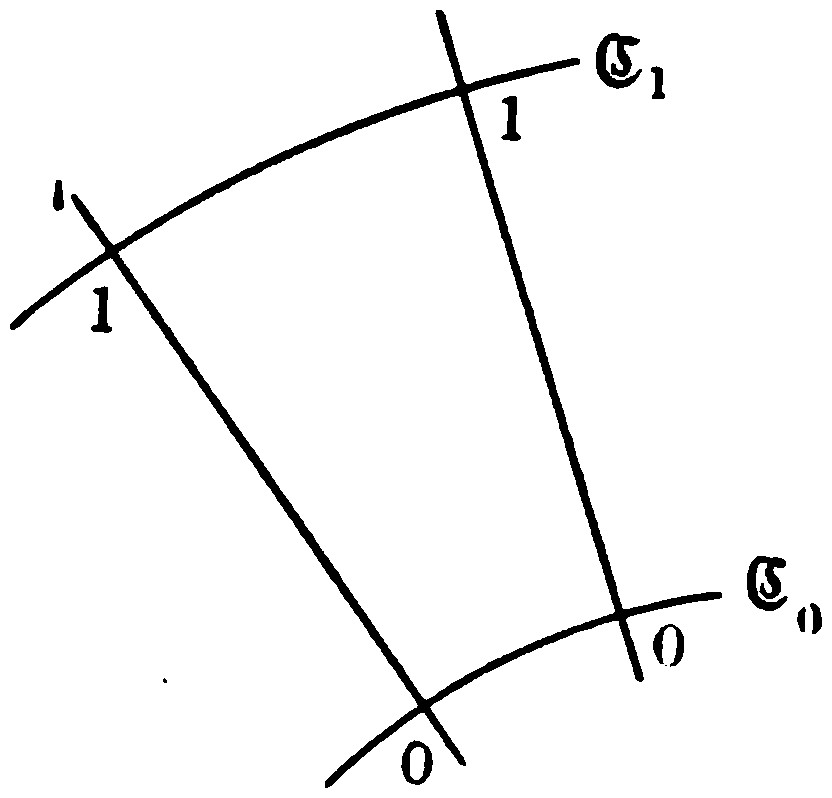
\includegraphics[width=\linewidth,height=32mm,keepaspectratio]{fig_assets/fig01_src_clean_x8.png}
\end{minipage}\hfill
\begin{minipage}[c]{0.49\linewidth}\centering
\end{minipage}
\end{center}

Thus, if on the extremals of the field which cut the curve $\mathfrak{C}_0$ transversally one bounds off such arcs 01 that the integrals $\overline{J}_{01}$ have the same value, then the locus of the points 1 is again a regular curve, which is cut transversally by the extremals of the field. (Compare Fig.~1, in which, as also in most later figures, the extremals appear as straight lines, and the transversal position is indicated by a right-angled intersection.)

In the result obtained one recognizes the generalization of the well-known theorem of \textsc{Gauss}, that a family of equal-length geodesic arcs which stand perpendicular to the line containing their initial points
% src-pdfpage=0071
% src-break=0071
also cut the locus of their endpoints at right angles; for (\S~11) in geodesic lines the transversal position coincides with the perpendicular position.

\begin{center}{\large \S~16.}\end{center}

Let the integrand $F(x,y,x',y')$ be regular and different from zero, say positive, either a) in all elements of the arc $\mathfrak{B}$ corresponding to the direction of increasing $t$, or b) in all line elements issuing from points of it in arbitrary directions. The function $F$ retains these properties, in case a), for all elements which issue from points of the field and are inclined sufficiently little from the indicated elements of the arc $\mathfrak{B}$, and, in case b), for all elements issuing from points of the field, provided that the field is sufficiently restricted. For by \S~3 one can assume for each single line element
\[
x'^2+y'^2=1,
\quad x'=\cos\varphi,
\quad y'=\sin\varphi;
\]
then $\varphi$ is the inclination of the element to the $+x$-axis, measured in the positive sense of rotation (\S~4), and $F$ is a regular function of $x,y,\varphi$, if $F(x,y,x',y')$ is regular in the line element characterized by $x,y,\varphi$. From this follows the assertion just stated, since a function regular at one place retains this property for a certain neighborhood of the place.

Under the narrower as under the wider assumption, one now has
\[
\frac{\partial u}{\partial t}=F(\xi,\eta,\xi_t,\eta_t)
\]
different from zero inside the field; for every system of values $(t,a)$ belonging to it, one can therefore, if the curve $\mathfrak{C}_0$ as before is cut transversally by the extremals of the field, calculate from the equation
\[
u=\int_{t_0}^{t}F(\xi,\eta,\xi_t,\eta_t)dt
\]
the quantity $t$ and hence also $x$ and $y$ as regular functions of $u$ and $a$; since the functional determinant
\[
\frac{\partial(t,a)}{\partial(u,a)}=1:\frac{\partial u}{\partial t}
\]
is different from zero, the same holds for
% src-pdfpage=0072
% src-break=0072
\begin{equation}\tag{36}
\frac{\partial(x,y)}{\partial(u,a)}
=\frac{\partial(\xi,\eta)}{\partial(t,a)}\frac{\partial(t,a)}{\partial(u,a)}
=\Delta:\frac{\partial u}{\partial t}
=\frac{\Delta}{F(\xi,\eta,\xi_t,\eta_t)}.
\end{equation}
If one imagines the expressions for $x$ and $y$ in terms of $u$ and $a$ introduced into the function $F(x,y,dx,dy)$, and sets
\[
v=a,
\quad \frac{dv}{du}=s,
\]
then one obtains
\[
F(x,y,dx,dy)=G(u,v,du,dv)=g(u,v,s)du,
\]
\[
J=\int G(u,v,u',v')dt;
\]
then $G$, and by \S~5 also, as long as $du$ does not vanish, $g(u,v,s)$, is regular in the same line elements as $F$.

Along the extremals of the field one has now
\[
v=a=\text{const.},\quad s=0,
\]
and since $F$ is positive, $u$ increases in the direction of increasing $t$; hence one has
\[
u=\int_0^1G(u,v,du,0)=\int_0^1g(u,v,0)du,
\]
where the function $g$ is to be formed corresponding to a positive value of $du$. Differentiating with respect to $u$ and remembering that 0, as the intersection of the curve $\mathfrak{C}_0$ and a line $v=\text{const.}$, is independent of $u$, the identity follows
\[
1=g(u,v,0),
\]
or, for $du>0$,
\[
G(u,v,du,0)=du.
\]

A further determination of the function $g$ is obtained when the fact that, according to \S~15, all lines $u=\text{const.}$ are cut transversally by the extremals $v=\text{const.}$ is expressed in the variables $u,v$. Namely, if the systems of values
\[
x,y,x',y';\quad u,v,u',v',
\]
in which the derivatives are taken with respect to an arbitrary parameter, represent the same line element, then the identities
\[
F(x,y,x',y')=G(u,v,u',v'),
\]
\[
x'=x_u u'+x_v v',\quad y'=y_u u'+y_v v',
\]
\[
u'=u_xx'+u_yy',\quad v'=v_xx'+v_yy',
\]
hold, and one can differentiate the first of them with respect to $x'$, $y'$; one then obtains
% src-pdfpage=0073
% src-break=0073
\[
F_{x'}=G_{u'}\frac{\partial u'}{\partial x'}+G_{v'}\frac{\partial v'}{\partial x'}
=u_xG_{u'}+v_xG_{v'},
\quad F_{y'}=u_yG_{u'}+v_yG_{v'}.
\]
On the other hand, for progress in an arbitrary direction, one has
\[
Dx=x_uDu+x_vDv,
\quad Dy=y_uDu+y_vDv,
\]
and therefore the identity follows
\[
F_{x'}Dx+F_{y'}Dy
=\{G_{u'}(u_xx_u+u_yy_u)+G_{v'}(v_xx_u+v_yy_u)\}Du+\cdots,
\]
or, since evidently
\[
\frac{\partial u}{\partial u}=u_xx_u+u_yy_u=1,
\quad
\frac{\partial v}{\partial u}=v_xx_u+v_yy_u=0,
\]
and two more similar equations hold, the identity
\[
F_{x'}Dx+F_{y'}Dy=G_{u'}Du+G_{v'}Dv.
\]
By \S~15 this quantity vanishes when $D$ denotes progress along the curve $u=\text{const.}$, while the derivatives refer to the extremals of the field; the equation
\[
G_{u'}Du+G_{v'}Dv=(g-sg_s)Du+g_sDv=0
\]
must therefore be fulfilled by the assumption $s=0$, $Du=0$, and one obtains
\[
g_s(u,v,0)=0.
\]
According to the found value of $g(u,v,0)$, the Taylor development of the function $g$ therefore receives, when $\theta$ belongs to the segment from 0 to $+1$, the form
\begin{equation}\tag{37}
g(u,v,s)=1+\frac{s^2}{2}g_{ss}(u,v,\theta s).
\end{equation}
This equation holds under assumption a) as long as $|s|$ does not exceed a certain positive quantity, and under assumption b) for every finite value of $s$. Evidently the preceding development remains valid when $\mathfrak{C}_0$ degenerates into a point.



\begin{center}
{\small Fig.~2.}\par\vspace{1mm}
\begin{minipage}[c]{0.47\linewidth}\centering
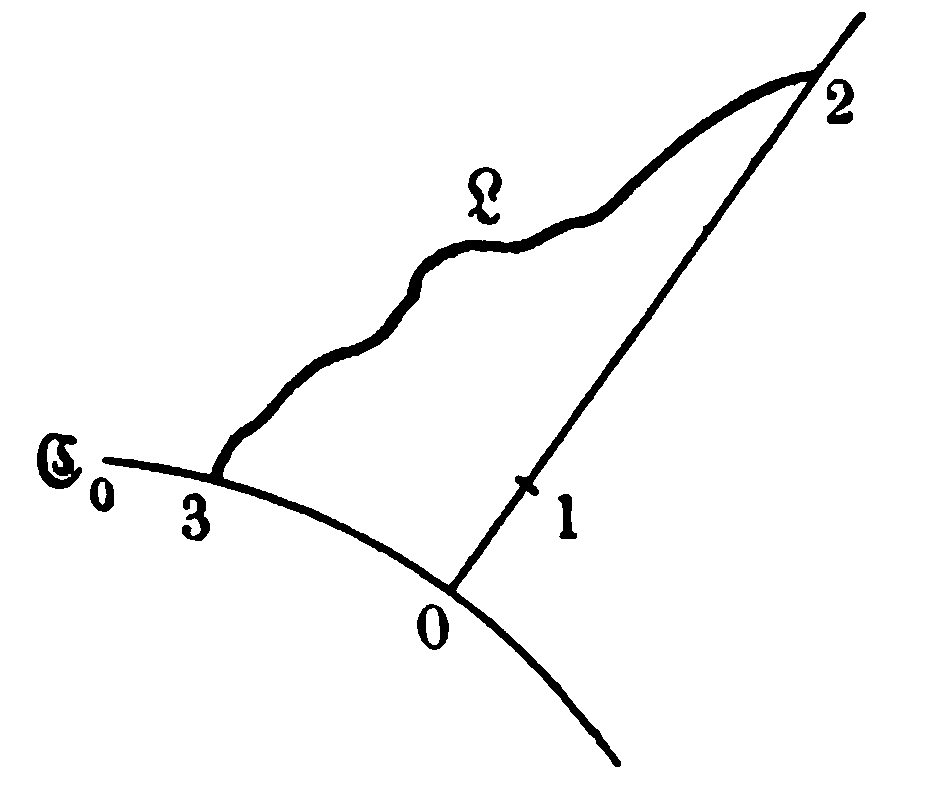
\includegraphics[width=\linewidth,height=32mm,keepaspectratio]{fig_assets/fig02_src_clean_x8.png}
\end{minipage}\hfill
\begin{minipage}[c]{0.49\linewidth}\centering
\end{minipage}
\end{center}

Let now (Fig.~2) 12 be any arc $\mathfrak{B}$ belonging to the field, 0 as before the intersection point of the extremal $\mathfrak{E}$ containing it with $\mathfrak{C}_0$, and 3 a fixed point of the latter curve, which is connected with 2 by a curve $\Omega$. Let this curve not leave the field; along it let $x,y$ be functions of a parameter $\tau$ increasing in the direction of integration, such that the integral
% src-pdfpage=0074
% src-break=0074
\[
J_{32}=\int_{\tau_3}^{\tau_2}F\left(x,y,\frac{dx}{d\tau},\frac{dy}{d\tau}\right)d\tau
=\int_{\tau_3}^{\tau_2}G\left(u,v,\frac{du}{d\tau},\frac{dv}{d\tau}\right)d\tau
\]
has a definite finite value, and the equation
\begin{equation}\tag{38}
\int_{\tau_3}^{\tau_2}\frac{du}{d\tau}d\tau
=\left.u\right|_3^2
=\left.u\right|_0^2
\end{equation}
holds. Then evidently
\begin{equation}\tag{39}
J_{32}-\overline{J}_{02}
=\int_3^2\left[G\left(u,v,\frac{du}{d\tau},\frac{dv}{d\tau}\right)-\frac{du}{d\tau}\right]d\tau;
\end{equation}
as soon as $du/d\tau$ is positive, the integrand can by (37) be written
\begin{equation}\tag{40}
\frac{s^2}{2}g_{ss}(u,v,\theta s)\frac{du}{d\tau};
\end{equation}
if $du/d\tau$ is negative or zero, then the integrand, just as $G$, is positive.

In order to decide the sign of this integral, one need not form the function $g$, which would often be difficult, but can proceed from the above linear relations between $x',y',u',v'$; the twice-repeated application of them gives
\[
\frac{\partial^2G}{\partial v'^2}=G_{v'v'}=F_{x'x'}x_v^2+2F_{x'y'}x_vy_v+F_{y'y'}y_v^2.
\]
Now from the identity
\[
F=x'F_{x'}+y'F_{y'},
\]
by differentiating with respect to $x'$ and $y'$, there follows
\[
x'F_{x'x'}+y'F_{x'y'}=x'F_{y'x'}+y'F_{y'y'}=0;
\]
if one recalls that $x'$ and $y'$ do not both vanish, it follows that one of the quantities
\[
F_{x'x'}:y'^2,
\quad F_{y'y'}:x'^2
\]
has a finite value $F_1(x,y,x',y')$, for which the equations
\[
F_{x'x'}=F_1y'^2,
\quad F_{x'y'}=-x'y'F_1,
\quad F_{y'y'}=x'^2F_1,
\quad F_1dt=\frac{f_{pp}dx}{x'^4}
\]
hold. Substituting these values into the expression $G_{v'v'}$, one obtains
% src-pdfpage=0075
% src-break=0075
\[
G_{v'v'}=F_1(x_vy'-y_vx')^2,
\]
and since
\[
G=u'g\left(u,v,\frac{v'}{u'}\right),
\]
it follows, for non-vanishing $u'$,
\[
\frac{g_{ss}(u,v,s)}{u'}=F_1(x_vy'-y_vx')^2,
\]
or, according to the linear equations existing between $x',y'$ and $u',v'$,
\[
\frac{g_{ss}(u,v,s)}{u'}=F_1\,(x_vy_u-x_uy_v)^2u'^2,
\]
and the parenthesis appearing on the right is different from zero by (36).

It is now assumed, for each of the cases a) and b), that $F_1$ has a constant sign and does not vanish in exactly those line elements for which, in each of these cases, $F$ is regular. A consideration like that carried out at the beginning of this paragraph shows that the stated property of $F_1$ in case a) need be assumed only for the elements of the arc $\mathfrak{B}$, and in case b) only for the elements issuing from its points. Along this arc $s=0$; if therefore $|s|$ along the curve $\Omega$ does not exceed a certain constant, then under assumption a) the quantities
\[
g_{ss}(u,v,\theta s),
\quad \int\frac{s^2}{2}g_{ss}(u,v,\theta s)du
\]
have the same sign as $F_1$, and $u'$ remains always positive; the quantity
\begin{equation}\tag{41}
G\left(u,v,\frac{du}{d\tau},\frac{dv}{d\tau}\right)-\frac{du}{d\tau}
\end{equation}
is always representable in the form (40) and likewise has the sign in common with $F_1$. If, on the other hand, $du/d\tau$ ceases in places to be positive, assumption b) is introduced; then for $u'>0$ the equation holds
\[
G(u,v,u',v')-u'=\frac{s^2}{2}g_{ss}(u,v,\theta s)u'
=\frac{v'^2}{2u'}g_{ss}(u,v,\theta s).
\]
If therefore the line element $(u,v,u',v')$ turns about a fixed point and $u'$ converges to zero from the positive side, then the left side approaches the limit $G(u,v,0,v')$, while the right side has the sign of $F_1$; the latter must
% src-pdfpage=0076
% src-break=0076
therefore agree with that of the integrand $G$ or $F$, which we assume to be positive, that is, $F_1$ is also positive. The quantity (41) is therefore positive for positive values of $du/d\tau$ and vanishes only for $s=0$; for negative or vanishing values of $du/d\tau$ it is evidently positive. The same therefore holds of the difference $J_{32}-\overline{J}_{02}$, as soon as equation (38) is correct and the integral representation (39) has a meaning.

\begin{center}{\large \S~17.}\end{center}

The concept of the extremum must be determined more precisely by specifications concerning the totality of all those curves which one intends to draw into comparison. The general conception of an extremum entails that one first compares neighboring curves; for the neighborhood we introduce the following definitions. If 12 is any plane arc, and if the arc $\Omega$ lies entirely in the interior of that surface which is covered by a circle of constant radius $\rho$ whose center traverses the arc 12, then we say that all curves $\Omega$ for which the associated quantities $\rho$ do not exceed a certain constant belong to a wider neighborhood of the arc 12. If there is still a positive constant $\rho_1$ of such a character that every tangent of the arc $\Omega$ forms, with at least one tangent of the arc 12 whose point of contact is separated from that of the former by less than $\rho$, an angle smaller than $\rho_1$, then we say that the arc $\Omega$ lies in a narrower neighborhood of the arc 12, as soon as $\rho$ and $\rho_1$ remain below certain constants. These definitions can evidently be transferred at once to space curves. Further, if the difference of the integrals $J$ formed along the two arcs has constant sign as soon as $\Omega$ lies in a wider neighborhood of the arc 12, then we say that the arc 12 gives a strong extremum of the integral $J$. If, on the other hand, that difference has a fixed sign only when $\Omega$ lies in a narrower neighborhood of 12, then we say that a weak extremum occurs. In the latter case a narrower domain of curves $\Omega$ has evidently been drawn into comparison with the arc 12 than in the first.

But in order to be able to prove an extremum, we must assume for the curves $\Omega$ certain continuity properties
% src-pdfpage=0077
% src-break=0077
which in essence amount to the fact that along these curves integrals of the form $J$ can be formed and treated according to the ordinary rules of operation of the infinitesimal calculus. To be able to formulate such properties exactly, we consider in general a function $\varphi(\tau)$ which in an arbitrarily bounded interval $\mathfrak{J}$ has the following properties. Let it be continuous, and let the quotient
\[
\frac{\varphi(\tau+\varepsilon)-\varphi(\tau)}{\varepsilon}
\]
approach, when $\varepsilon$ is positive and decreases without limit, for every value of $\tau$ a definite finite limit $\varphi'(\tau)$. It need not be excluded that the quotient
\[
\frac{\varphi(\tau-\varepsilon)-\varphi(\tau)}{-\varepsilon}
\]
approaches another limit or no limit at all. The quantity $\varphi'(\tau)$ we call, as has sometimes been done, the forward derivative. For it, just as for the ordinary concept of derivative, the theorem holds that the continuous function $\varphi(\tau)$ in the interval from $\tau_0$ to $\tau_1$ must be constant if the forward derivative in this segment everywhere has the definite value zero; for if one sets
\[
\psi(\tau)=\varphi(\tau)+\alpha(\tau-\tau_0),
\quad \theta(\tau)=\varphi(\tau)-\alpha(\tau-\tau_0)
\]
and understands by $\alpha$ a positive constant, then $\psi(\tau)$ has the forward derivative $\alpha$, $\theta(\tau)$ the forward derivative $-\alpha$; the first function therefore increases, the latter decreases between $\tau_0$ and $\tau_1$, so that, if $\tau_1>\tau_0$, the inequalities
\[
\psi(\tau_1)>\psi(\tau_0),
\quad \theta(\tau_1)<\theta(\tau_0),
\]
\[
\varphi(\tau_1)+\alpha(\tau_1-\tau_0)>\varphi(\tau_0),
\quad \varphi(\tau_1)-\alpha(\tau_1-\tau_0)<\varphi(\tau_0),
\]
\[
\alpha(\tau_1-\tau_0)>\varphi(\tau_0)-\varphi(\tau_1)>-\alpha(\tau_1-\tau_0)
\]
hold. The last of them gives, since $\alpha$ can be arbitrarily small, $\varphi(\tau_1)=\varphi(\tau_0)$, by which the assertion is proved.

Apart from this special case, suppose now that the function $\varphi'(\tau)$ has the following property. Its oscillation in any interval is the upper bound of the absolute values of the differences of any two values of the function attained in this interval; the total length of all parts of the interval $\mathfrak{J}$ within which the oscillation of $\varphi'(\tau)$ exceeds a positive constant
% src-pdfpage=0078
% src-break=0078
can always be made infinitely small. Then, according to \textsc{Riemann}, the function $\varphi'(\tau)$ is integrable, and the integral
\[
\Phi(\tau)=\int_{\tau_0}^{\tau}\varphi'(\tau)d\tau,
\]
whose interval of integration forms a part of $\mathfrak{J}$, is a finite continuous function of $\tau$. Further we assume that, when $\varepsilon$ is positive,
\[
\lim_{\varepsilon=0}\varphi'(\tau+\varepsilon)=\varphi'(\tau);
\]
thereby the discontinuities of the function $\varphi'(\tau)$ are restricted in a certain way, but it is still, for example, possible that arbitrarily near a point of discontinuity infinitely many others lie. Under this assumption the quantity $\varphi'(\tau)$ is positive along a finite segment if this holds at a single place. Further one obtains for $\varepsilon>0$
\[
\Phi(\tau+\varepsilon)-\Phi(\tau)
=\int_{\tau}^{\tau+\varepsilon}\varphi'(\tau)d\tau=M\varepsilon,
\]
where $M$ lies between the upper and lower bounds of the values which $\varphi'(\tau)$ takes between $\tau$ and $\tau+\varepsilon$; by the preceding equation $M$ converges to $\varphi'(\tau)$ when $\varepsilon$ vanishes. The quantity $\Phi(\tau)$ therefore has the forward derivative
\[
\Phi'(\tau)=\varphi'(\tau),
\]
the difference $\Phi(\tau)-\varphi(\tau)$ is constant, and since $\Phi(\tau_0)$ vanishes, one obtains
\[
\Phi(\tau)=\varphi(\tau)-\varphi(\tau_0)=\int_{\tau_0}^{\tau}\varphi'(\tau)d\tau.
\]
Thus the ordinary fundamental relation between differentiation and integration holds when the first operation is referred to forward derivatives.

Now let $x$ and $y$ along the curve $\Omega$ be functions of the parameter $\tau$ which have the properties of the function $\varphi(\tau)$, hence possess integrable forward derivatives, which we denote by the usual differential symbols; at the same time let the sum
\[
\left(\frac{dx}{d\tau}\right)^2+
\left(\frac{dy}{d\tau}\right)^2
\]
always lie above a positive constant. With this, since $\varphi'(\tau)$ need not be continuous, it is by no means excluded that the
% src-pdfpage=0079
% src-break=0079
curve $\Omega$ has corners in a finite or infinite number; but at every point it has a definite direction corresponding to increasing values of $\tau$. If $\Omega$ lies in a sufficiently bounded, narrower or wider neighborhood of the arc $\mathfrak{B}$, according as assumption a) or b) of the preceding paragraph holds, then in the first case every system of values
\[
\left(x,y,\frac{dx}{d\tau},\frac{dy}{d\tau}\right)
\]
differs arbitrarily little from one which represents an element of the curve $\mathfrak{E}$; in the second case $F$ is regular for arbitrarily directed line elements issuing from points of the field; in both cases this therefore holds for every system of values defined by the curve $\Omega$,
\[
\left(x,y,\frac{dx}{d\tau},\frac{dy}{d\tau}\right),
\]
and the oscillation, corresponding to a variable interval of the argument $\tau$, of the quantity
\[
F\left(x,y,\frac{dx}{d\tau},\frac{dy}{d\tau}\right)
\]
becomes infinitely small with the oscillation present in the same interval of the quantities
\[
\frac{dx}{d\tau},\quad \frac{dy}{d\tau}.
\]
Set further
\[
F\left(x,y,\frac{dx}{d\tau},\frac{dy}{d\tau}\right)=\Theta(\tau),
\]
then it is evident, if $\varepsilon>0$, that
\[
\Theta(\tau)=\lim_{\varepsilon=0}\Theta(\tau+\varepsilon),
\]
since such an equation holds for $dx/d\tau$ and $dy/d\tau$; thus $\Theta(\tau)$ has all the properties of $\varphi'(\tau)$ assumed above, is integrable, and gives the equation
\[
\frac{d}{d\tau}\int_{\tau_0}^{\tau}\Theta(\tau)d\tau
=\frac{d}{d\tau}\int_{\tau_0}^{\tau}F\left(x,y,\frac{dx}{d\tau},\frac{dy}{d\tau}\right)
=F\left(x,y,\frac{dx}{d\tau},\frac{dy}{d\tau}\right),
\]
which corresponds to the ordinary rules of integral calculus. The same properties as $F$ are possessed, if $\Phi(x,y)$ is a function of the coordinates regular along the curve $\Omega$, by the quantity
\[
\frac{d\Phi}{d\tau}=\Phi_x\frac{dx}{d\tau}+\Phi_y\frac{dy}{d\tau};
\]
if one applies these remarks to the quantities $u,v$, which are regular functions of the coordinates, it follows that also the quantities
% src-pdfpage=0080
% src-break=0080
\[
G\left(u,v,\frac{du}{d\tau},\frac{dv}{d\tau}\right),
\quad \frac{du}{d\tau},\quad \frac{dv}{d\tau}
\]
have the properties of $\varphi'(\tau)$, and in particular the difference of the first two quantities along a finite segment is positive if this occurs at a single place. Further it follows that equations (38), (39) are correct under the introduced assumptions, if we always refer the sign of differentiation with respect to $\tau$ to the forward derivatives. This is quite natural in the formation of $J_{32}$, since integration is performed in the direction of increasing $\tau$.

On the basis of these developments it is now to be rigorously proved that the quantity
\[
J_{32}-\overline{J}_{02}
=\int_3^2\left[G\left(u,v,\frac{du}{d\tau},\frac{dv}{d\tau}\right)-\frac{du}{d\tau}\right]d\tau
\]
has the sign in common with $F_1$ and vanishes only when the curves $\Omega$ and $\mathfrak{B}$ coincide completely. This is clear without further argument in case a), since the integrand along the whole interval of integration can be replaced by
\begin{equation}\tag{42}
\frac{s^2}{2}g_{ss}(u,v,\theta s)\frac{du}{d\tau}
\end{equation}
and the quantity $g_{ss}du$ does not vanish by assumption. In case b) the integrand is likewise never negative, and, if $J_{32}-\overline{J}_{02}$ is to vanish, the quantity $dv/d\tau$ can in any case not be different from zero where $du/d\tau$ is positive; for in this case the integrand is again representable in the form (42), hence positive. But if $du/d\tau$ becomes negative at some place, then the integrand of the above integral is again positive; since the latter, as noted above, remains positive along a finite segment when this occurs at a single place, the integral $J_{32}-\overline{J}_{02}$ can surely vanish only when $v$ is constant along the curve $\Omega$, so that the latter coincides with $\mathfrak{B}$.

Therewith the proof of the extremum is completed, whether one compares the arc 02 with all arcs which have the same endpoints, or with all arcs going from the curve $\mathfrak{C}_0$ to the point 2. If, however, the curve $\mathfrak{C}_0$ contracts
% src-pdfpage=0081
% src-break=0081
into the point 0, so that all extremals of the field pass through it, then it must still be specially assumed for the curve $\Omega$ that it always remains inside the domain simply covered by the extremals of the field (Fig.~3). This is achieved, for example, by making all curves $\Omega$ have in common with the curve $\mathfrak{E}$ an arbitrarily small, constant piece 01 (Fig.~4); then



\begin{center}
\begin{minipage}[c]{0.47\linewidth}\centering
{\small Fig.~3.}\par\vspace{1mm}
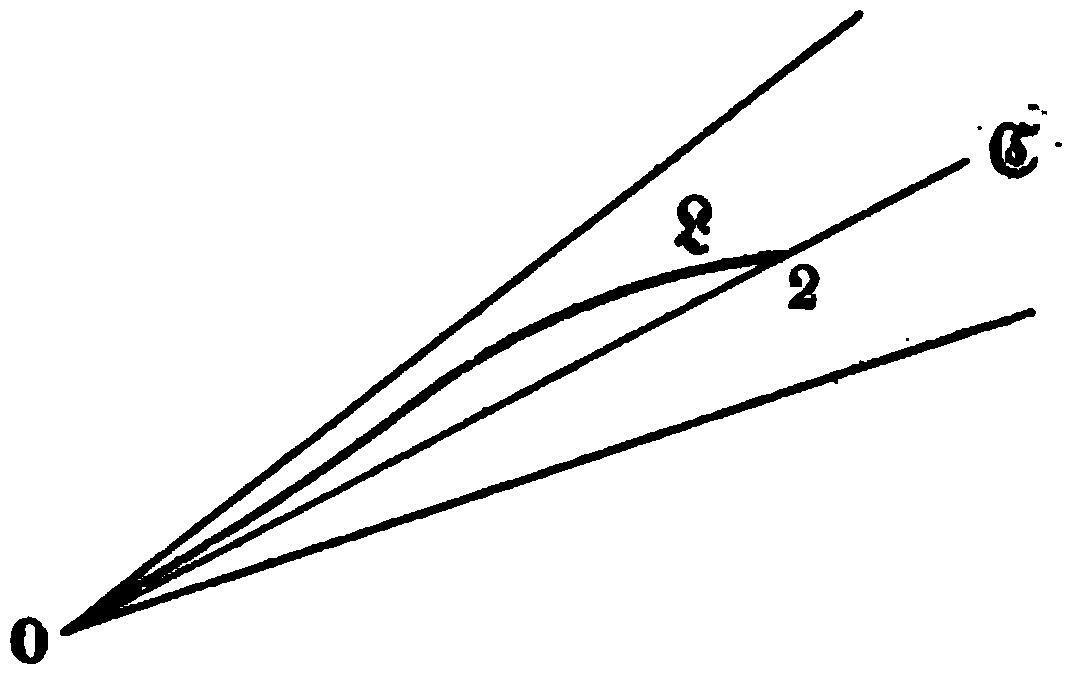
\includegraphics[width=\linewidth,height=24mm,keepaspectratio]{fig_assets/fig03_src_clean_x8.png}\par\vspace{1mm}
\end{minipage}\hfill
\begin{minipage}[c]{0.47\linewidth}\centering
{\small Fig.~4.}\par\vspace{1mm}
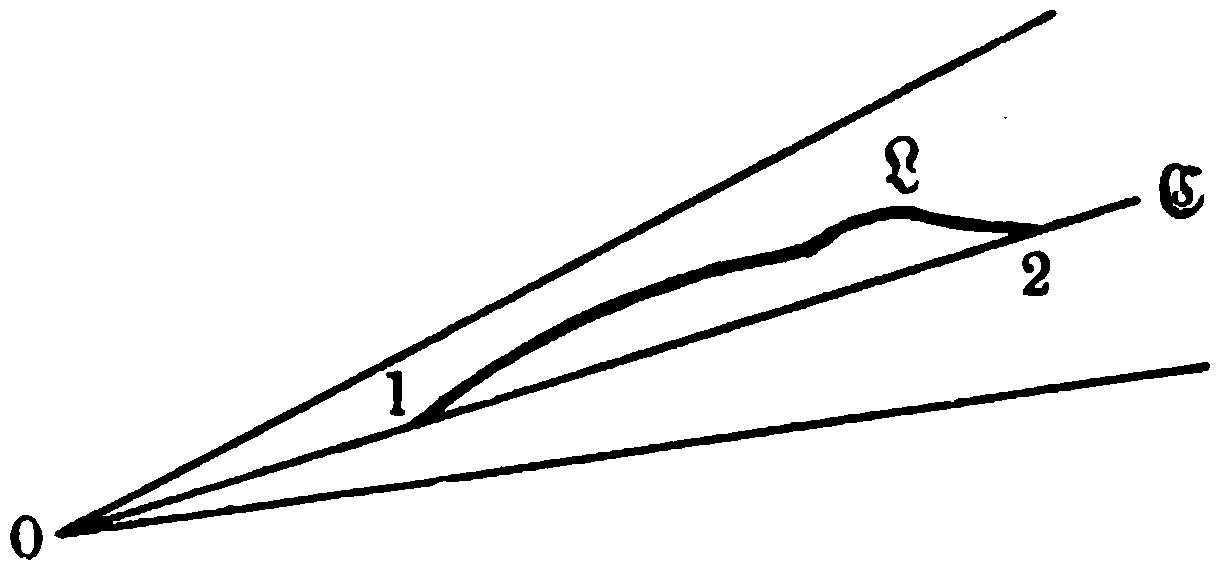
\includegraphics[width=\linewidth,height=24mm,keepaspectratio]{fig_assets/fig04_src_clean_x8.png}\par\vspace{1mm}
\end{minipage}
\end{center}
\[
J_{32}-\overline{J}_{02}=J_{02}-\overline{J}_{02}=\overline{J}_{01}+J_{12}-\overline{J}_{02}=J_{12}-\overline{J}_{12},
\]
and for the arc 12 the extremum relative to all arcs with the same endpoints is secured in the unrestricted sense of the above definition. This also holds when the extremals become singular at the point 0, provided that the assumptions stated in \S~15 for this case hold. Finally one easily sees that the argument is not changed if the point 2, as endpoint of the arc $\Omega$, is left variable on a curve $\mathfrak{C}_2$ which cuts the extremals of the field transversally, while 0 is held fixed, so that the direction of integration, contrary to the previous assumption, leads from the fixed point to the fixed curve.

The extent of the field within which the curves $\Omega$ must run has been restricted by us in \S~16 so that the assumptions a), b) can be transferred from points or elements of the arc $\mathfrak{E}$ to all extremals of the field, and likewise in \S~15 so as to ensure that the curves $u=\text{const.}$ remain regular and cut each extremal of the field only once. If these properties, always attainable by restricting the field, are demonstrable in a special problem for a definite field of finite extent, then our argument holds for every curve $\Omega$ running in this field, and then supplies more than the proof of the extremum; for the latter is already secured when only a field of arbitrarily small extent has been constructed.
% src-pdfpage=0082
% src-break=0082

We summarize the most important of the results obtained in the following way. 1. \textsc{Jacobi}'s condition. A nowhere singular piece of an extremal with endpoints 0, 2 is to be surrounded by a field. 2. \textsc{Legendre}'s condition. Either a) in all elements of the arc 02, which is traversed in the direction from 0 to 2, or b) in all line elements issuing from points of it, the quantity $F_1$ or $f_{pp}dx$ is to have a fixed sign, without vanishing, and $F$ is to be regular and different from zero. Then the arc 02 supplies an extremum of the integral $J$, both in comparison with all curves $\Omega$ with the same endpoints, and with all those which connect the curve $\mathfrak{C}_0$, issuing from the point 0 and transversally intersected by the extremals of the field, with the point 2. The strong or weak extremum is secured according as assumption b) or a) is made; a maximum or a minimum occurs according as $F_1$ is negative or positive.

% src-pdfpage=0082
% src-break=0082
\begin{center}{\large \S~18.}\end{center}

\noindent\textbf{Examples. Problem I (\S~9).} Here one has
\[
Fdt=\sqrt{x'^2+y'^2}\,dt,
\]
the square root is positive, hence
\[
y'^2F_1=F_{x'x'}=\frac{\partial}{\partial x'}
\left(\frac{x'}{\sqrt{x'^2+y'^2}}\right)
=\frac{y'^2}{\left(\sqrt{x'^2+y'^2}\right)^3},
\]
\[
F_1=\left(\frac{1}{\sqrt{x'^2+y'^2}}\right)^3
\]
with likewise positive square root. Further,
\[
Fdt=f\,dx,\quad f=\sqrt{1+p^2},\quad
f_{pp}=\left(\frac{1}{\sqrt{1+p^2}}\right)^3,
\]
where the square root has the sign of $dx$, so that for every arc element $f_{pp}dx$, just as $F_1$, is positive. Thus \textsc{Legendre}'s sign condition for the strong minimum is fulfilled.

In order to investigate whether a straight segment 12 gives the shortest line between 1 and 2, assume (Fig.~5) that $\Omega$ is any line 12 with the continuity properties specified in \S~17, giving the arc integral $J_{12}$; the length
% src-pdfpage=0083
% src-break=0083
of the segment 12 is $\overline{J}_{12}$. Let 0 further be a point of the line 12 which does not belong to the line $\Omega$ and lies outside the segment 12; take it as the origin of the rectangular and polar coordinates, putting
\[
x=t\cos v,\quad y=t\sin v
\]
and choose the constants $\alpha,\beta$ so that
\[
0<\alpha<\beta
\]
and the curve $\Omega$ runs wholly in the interior of the annular region between the circles $t=\alpha$, $t=\beta$. This region, which is covered exactly once by the extremals $v=\text{const.}$, can be regarded as a field of the straight segment 12, since in it the quantity
\[
\frac{\partial(x,y)}{\partial(t,v)}
=
\begin{vmatrix}
\cos v & \sin v\\
-t\sin v & t\cos v
\end{vmatrix}
=t
\]
is different from zero.



\begin{center}
{\small Fig.~5.}\par\vspace{1mm}
\begin{minipage}[c]{0.47\linewidth}\centering
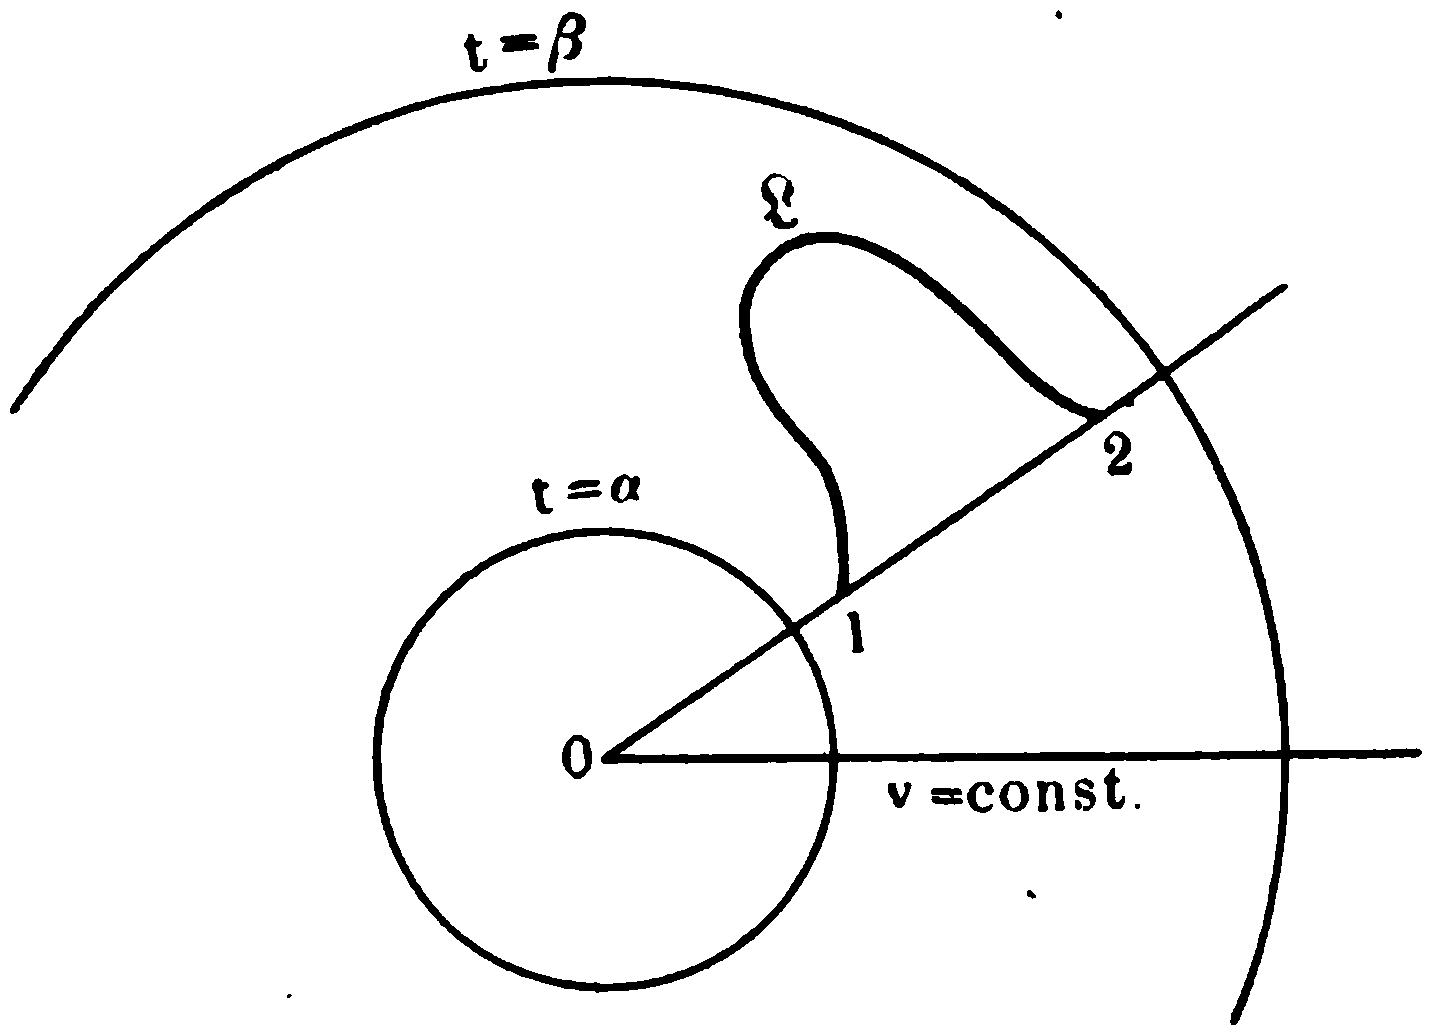
\includegraphics[width=\linewidth,height=32mm,keepaspectratio]{fig_assets/fig05_src_clean_x8.png}
\end{minipage}\hfill
\begin{minipage}[c]{0.49\linewidth}\centering
\end{minipage}
\end{center}

The curves $\mathfrak{C}_0$ of the general theory correspond to the circles $t=\text{const.}$, each of which cuts the extremals of the field in one point; $u$ is the length of a straight line $v=\text{const.}$ measured from the circle $t=\alpha$, and hence
\[
u+\alpha=t,\quad
Fdt=\sqrt{dt^2+t^2dv^2}=\sqrt{du^2+(u+\alpha)^2dv^2}
=G(u,v,du,dv),
\]
\[
g(u,v,s)=\sqrt{1+(u+\alpha)^2s^2},
\]
where the last square root also is positive, since the expression $g$ is formed only for the case $du>0$. In the difference
\[
J_{12}-\overline{J}_{12}
=
\int_{\tau_1}^{\tau_2}
\left[
G\left(u,v,\frac{du}{d\tau},\frac{dv}{d\tau}\right)
-\frac{du}{d\tau}
\right]d\tau
\]
the integrand is of itself positive as soon as $\frac{du}{d\tau}$ is negative or vanishes, which characterizes the parts of the curve $\Omega$ in which the radius $t$ decreases. If $\frac{du}{d\tau}$ is positive, then the integrand can be written
% src-pdfpage=0084
% src-break=0084
\[
\sqrt{1+(u+\alpha)^2s^2}-1,
\]
and is therefore likewise not negative and vanishes only for $s=0$. If at any place $s$ were different from zero, or the integrand were positive, then by \S~17 the same would hold for a finite segment of the curve $\Omega$; the difference $J_{12}-\overline{J}_{12}$ could therefore vanish only if $du$ were positive everywhere and $s=0$. Apart from this case, one evidently has
\[
J_{12}>\overline{J}_{12},
\]
which proves the strong minimum, and even more.

Next let $\mathfrak{C}_1$ be any curve traversed from the point 1, so that $x_1,y_1$ are regular functions of a parameter $v$, and let $n$ be the direction of the normal, situated with respect to the direction of increasing $v$ as the $+y$-axis is to the $+x$-axis; putting then
\[
x=\xi(t,v)=x_1+t\cos(nx),\quad
y=\eta(t,v)=y_1+t\cos(ny),
\]
$v=\text{const.}$ is a normal of the curve $\mathfrak{C}_1$, and one has
\[
\Delta=\frac{\partial(\xi,\eta)}{\partial(t,v)}
=
\begin{vmatrix}
\cos(nx) & \dfrac{dx_1}{dv}+t\,\dfrac{d\cos(nx)}{dv}\\[1.1em]
\cos(ny) & \dfrac{dy_1}{dv}+t\,\dfrac{d\cos(ny)}{dv}
\end{vmatrix}.
\]
If in particular $v$ is the arc length on the curve $\mathfrak{C}_1$, then
\[
\cos(nx)=-\frac{dy_1}{dv},\quad \cos(ny)=\frac{dx_1}{dv},
\]
\[
\Delta=-1+t\left(
\frac{dx_1}{dv}\frac{d^2y_1}{dv^2}
-\frac{dy_1}{dv}\frac{d^2x_1}{dv^2}
\right)
=-1+\frac{t}{r},
\]
where $r$ denotes the radius of curvature at the point 1, taken positive or negative according as the centre of curvature lies in the direction $n$ or in the opposite one.

Now suppose that on some normal $v=\text{const.}$ the direction from 1 toward the point 2 agrees with $n$, so that $t_2$ is positive; then the straight segment 12, whose length is $t_2$, can be surrounded with a field in which $\Delta$ does not vanish, if either $r$ is negative or the inequality
\[
0<t_2<r
\]
holds, that is, always when the segment 12 does not contain the centre of curvature of the point 1 (Fig.~6). The extre-
% src-pdfpage=0085
% src-break=0085
mals of the field are the normals $v=\text{const.}$ which cut the curve $\mathfrak{C}_1$ transversally. The general theory therefore gives that the straight segment 12 supplies a strong minimum of the distance between $\mathfrak{C}_1$ and the point 2, and is shorter than every line $\Omega$ running in the field with the continuity properties stated above, which leads from the curve $\mathfrak{C}_1$ to the point 2. The quantity $u$ is the normal distance from the curve $\mathfrak{C}_1$; and one easily obtains the formula



\begin{center}
{\small Fig.~6.}\par\vspace{1mm}
\begin{minipage}[c]{0.47\linewidth}\centering
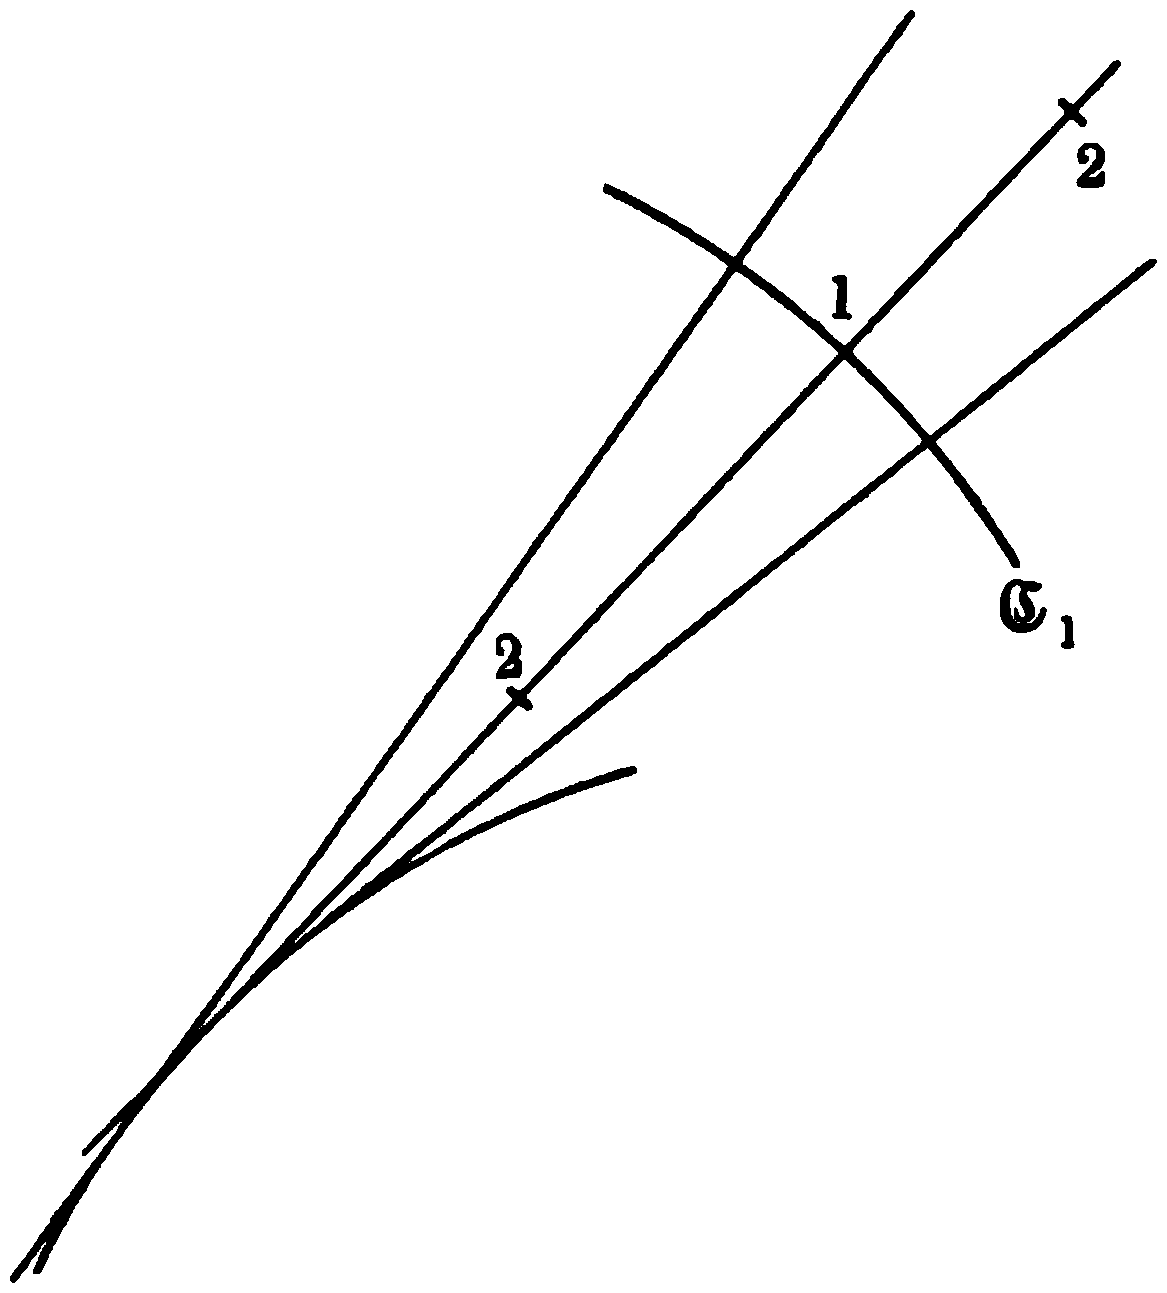
\includegraphics[width=\linewidth,height=32mm,keepaspectratio]{fig_assets/fig06_src_clean_x8.png}
\end{minipage}\hfill
\begin{minipage}[c]{0.49\linewidth}\centering
\end{minipage}
\end{center}

\[
\sqrt{dx^2+dy^2}
=
\sqrt{du^2+(u-r)^2dv^2}
=G(u,v,du,dv),
\]
to which the same conclusions can be attached as to the earlier transformation of the arc element.

\bigskip

\noindent\textbf{Problem III (\S~9).} If in the $wy$-plane $\Omega$ is any line drawn from the point 0 in the half-plane $y>0$ to the $w$-axis, of length $l$, along which $w,y$, as functions of a parameter $\tau$, have the properties of $\varphi(\tau)$ (\S~17), then it is to be proved that the area integral is smaller than the area of the semicircle of length $l$. If $\frac{dw}{d\tau}$ is negative in pieces, we consider the curve $\Omega^0$ which is defined by the equations
\[
y=\int_{\tau_0}^{\tau}\frac{dy}{d\tau}\,d\tau,\quad
w=\int_{\tau_0}^{\tau}\left|\frac{dw}{d\tau}\right|\,d\tau
\]
; if $\tau$ runs through the same interval as on the curve $\Omega$, this curve likewise has the length $l$ and the same continuity properties, since, as is easily seen, $|\varphi(\tau)|$ likewise possesses the properties required in \S~17 for $\varphi(\tau)$. The area integral of the curve $\Omega^0$ is finite and consists only of positive elements; evidently one has
% src-pdfpage=0086
% src-break=0086
\[
\int_{\tau_0}^{\tau}y\left|\frac{dw}{d\tau}\right|\,d\tau
\geqq
\int_{\tau_0}^{\tau}y\frac{dw}{d\tau}\,d\tau,
\]
that is, the area bounded by the curve $\Omega^0$ and the $w$-axis is not smaller than that bounded by the curve $\Omega$. It therefore remains only to show that the former is smaller than the area of the above designated semicircle; here we now have the advantage that in the integral
\[
J=\int y\sqrt{1-p^2}\,dx=\int y\,dw
\]
the square root is always to be taken positive. To the curve $\Omega^0$ there corresponds in the $xy$-plane a curve $\Omega_0$ along which, since $x$ is the arc of the curve $\Omega^0$, everywhere
\begin{equation}\tag{43}
\frac{dx}{d\tau}>0,\quad -1\leqq\frac{dy}{dx}\leqq +1;\quad x>0,\quad 0\leqq y\leqq x;
\end{equation}
thus it is not at all necessary to prove a strong extremum in the $xy$-plane; rather, only the curves characterized by these inequalities are to be brought into the comparison. \textsc{Legendre}'s condition for the maximum is fulfilled for all curves $\Omega_0$ under consideration insofar as for them the quantity



\begin{center}
\begin{minipage}[c]{0.47\linewidth}\centering
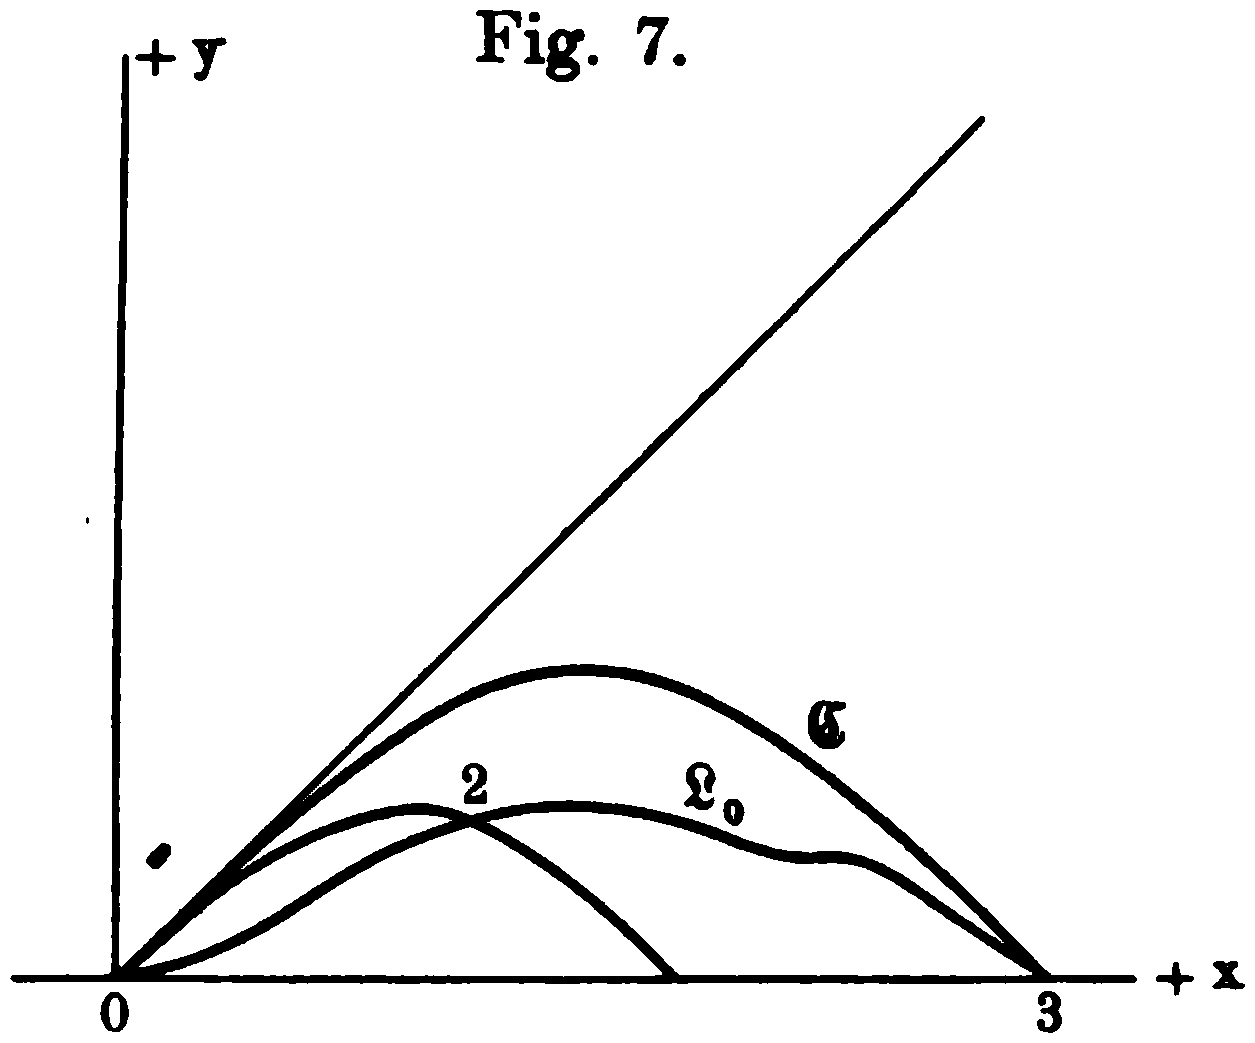
\includegraphics[width=\linewidth,height=32mm,keepaspectratio]{fig_assets/fig07_src_clean_x8.png}
\end{minipage}\hfill
\begin{minipage}[c]{0.49\linewidth}\centering
\end{minipage}
\end{center}

\[
f_{pp}\,dx=\frac{-y\,dx}{\left(\sqrt{1-p^2}\right)^3}
\]
is negative.

The octant of the $xy$-plane (Fig.~7) in which, according to the last inequalities (43), the curve $\Omega_0$ lies, is now covered exactly once by the extremals
\[
y=a\sin\frac{x}{a},\quad a>0,\quad p=\cos\frac{x}{a},
\]
on each of which one assumes
\begin{equation}\tag{44}
0\leqq\frac{x}{a}\leqq\pi
\end{equation}
; for if $x$ is held fixed, then
\[
\frac{\partial y}{\partial a}
=\sin\frac{x}{a}-\frac{x}{a}\cos\frac{x}{a}
\]
% src-pdfpage=0087
% src-break=0087
is always positive because of the inequality (44) holding for $x$. For $a=0$ one has $y=0$, whereas for $a=\infty$ one has $y=x$; the point $(x,y)$ therefore runs through all points of the straight line $x=\text{const.}$ belonging to that octant, and each once, when $a$ runs through all positive values. Further, one can put $x=t$, and then has
\[
\Delta=\frac{\partial(x,y)}{\partial(t,a)}
=\frac{\partial y}{\partial a},
\]
which quantity, as noted, is positive so long as $y$ does not vanish or become $=x$. If the points 0, 3 correspond to the values $x=0$ and $x=a\pi$, then every part of the extremal arc 03 containing neither endpoint is surrounded by a field; the endpoints themselves require special consideration, since at them $p=\pm1$, and the function $F$ therefore becomes singular.

Putting, according to the general theory in the case in which the curve $\mathfrak{C}_0$ contracts to the point 0,
\[
u=\int_0^x y\sqrt{1-p^2}\,dx
=a\int_0^x\sin^2\frac{x}{a}\,dx
=\frac{ax}{2}-\frac{a^2}{2}\sin\frac{x}{a}\cos\frac{x}{a},
\]
where the positive sign of the square root has been used, one easily verifies by means of the expressions
\[
F=y\sqrt{x'^2-y'^2},\quad
F_{x'}=\frac{yx'}{\sqrt{x'^2-y'^2}},\quad
F_{y'}=-\frac{yy'}{\sqrt{x'^2-y'^2}}
\]
the equations
\[
\frac{\partial u}{\partial a}
=
F_{x'}\frac{\partial x}{\partial a}
+
F_{y'}\frac{\partial y}{\partial a},
\quad
du=F_{x'}\,dx+F_{y'}\,dy.
\]
This differential $du$ can now vanish or become negative on no curve $\Omega_0$ between 0 and 3; for if $d$ refers to progress along the curve $\Omega_0$, while $x',y',p$ refer to the extremal of the field, then, since $dx$ is positive and $x=t$ is put for the extremal, so that $F_{x'}$ can be regarded as positive, one would obtain
\[
F_{x'}+F_{y'}\frac{dy}{dx}\leqq0,\quad
1+\frac{F_{y'}}{F_{x'}}\frac{dy}{dx}\leqq0,\quad
p\frac{dy}{dx}\geqq1,
\]
which by the second inequality (43) and the above given value of $p$ can occur only for $p=\pm1$, that is, at the points of the $x$-axis. The quantity $du:d\tau$ is therefore, between
% src-pdfpage=0088
% src-break=0088
the points 0 and 3, always positive, so that one can put everywhere
\[
dJ_{02}=du\left[1+\frac{s^2}{2}\,g_{ss}(u,v,\theta s)\right],
\]
whence, from the above recognized character of the expression $f_{pp}dx$, it follows that
\[
\frac{d(J_{02}-u)}{d\tau}<0.
\]

The transformation of the differential $dJ_{02}$ into the variables $u,v$ becomes impossible when
\[
dw=0,\quad dx=\pm dy,
\]
since then the integrand $F$ is singular. Nevertheless at such places, as the original definition
\[
J=\int y\,\frac{dw}{d\tau}\,d\tau
\]
teaches, $J_{02}$ remains a function $\varphi(\tau)$ in the sense of \S~17. Here evidently $dJ_{02}:d\tau$ vanishes, and for $du$ one finds
\[
du=dx(F_{x'}\pm F_{y'})=a\,dx\left(1\pm\cos\frac{x}{a}\right),
\]
so that $d(u-J_{02})$ remains positive also now. The quantity $u-J_{02}$ therefore increases when the point 2 runs from 0 to 3 along the curve $\Omega_0$.

Closer investigation is required, because of the singularity of the point 0, for the initial value of $u$. This is at first evidently zero if the inequality
\[
\left(\frac{dy}{d\tau}:\frac{dx}{d\tau}\right)^0<1
\]
holds; for then the quantity $a$, since it becomes infinite only for $x=y$, remains under a finite bound in the approach to the point 0 along the curve $\Omega_0$; the expression for $u$ therefore shows immediately that $u$ converges with $x$ to the limit zero. If, on the other hand, one has the equations
\[
\left(\frac{dy}{d\tau}:\frac{dx}{d\tau}\right)^0=1,\quad
\lim_{\tau=\tau_0}\frac{y}{x}=1,
\]
then the equation serving to define $a$, that is, if one puts
\[
\varphi(z)=\frac{\sin z-z}{z},
\]
% src-pdfpage=0089
% src-break=0089
the equation
\[
\frac{y}{x}=1+\varphi\left(\frac{x}{a}\right),
\]
teaches that one must have
\[
\left.\varphi\left(\frac{x}{a}\right)\right|^0=0.
\]
Now the quantity $\varphi(z)$ is negative so long as $z$ lies between 0 and $\pi$; from this it follows, since the inequality (44) holds, that
\[
\varphi\left(\frac{x}{a}\right)
\]
vanishes only when the equation
\[
\frac{x}{a}=0
\]
holds, which is thus proved for the point 0. This also holds evidently when the curve $\Omega_0$ has a finite piece in common with the straight line $y=x$ and 0 denotes the point at which the straight line and the curve separate. Substituting the obtained value $\frac{x}{a}$ into the equation
\[
u=\frac{a^2}{4}\left\{\frac{2x}{a}-\sin\frac{2x}{a}\right\}
=
\frac{1}{4}\left\{
\frac{(2x)^2}{3!}\cdot\frac{2x}{a}
-
\frac{(2x)^2}{5!}\left(\frac{2x}{a}\right)^3
+\cdots
\right\},
\]
one sees that in this case also the quantity $u$, as a function of $\tau$, begins with the value 0 at the place 0. Since the same is evidently true of $J_{02}$, one also has
\[
\left.u-J_{02}\right|_{\tau_0}=0,
\]
so the difference $u-J_{02}$ is, since it increases, positive as soon as the point 2, running along the arc $\Omega_0$, has left the straight line $y=x$; likewise the limiting value
\[
\left.u\right|^3-J_{03}=\overline{J}_{03}-J_{03}
\]
is positive. The lines $\Omega$ and $\Omega^0$, together with the $w$-axis, therefore enclose a smaller area than the semicircle of the same length.

The theorem that a closed curve always encloses a smaller area than a circle of the same length follows immediately from the result obtained, if the curve can be divided by two of its points 1 and 2 into two pieces of equal length in such a way that the straight segment 12 runs wholly in the interior; this segment can then be identified with the $w$-axis.

\bigskip

\noindent\textbf{Problem VI (\S~11).} Every piece of an extremal which does not contain the point of return can be surrounded with a field
% src-pdfpage=0090
% src-break=0090
by, for example, setting the quantity $a$ constant in the equations (17) and letting $b$ alone vary. The extremals of the field are then curves which arise one from the other by displacement parallel to the $x$-axis; hence, putting $t=p$, one has the equations
\[
\frac{\partial x}{\partial b}=1,\quad
\frac{\partial y}{\partial b}=0,\quad
\Delta=-\frac{dy}{dp},
\]
and by (18) $\Delta$ can vanish only at the point of return. Further one finds
\[
f_{pp}\,dx=-\frac{2yp(p^2-3)}{(1+p^2)^3}\,dx.
\]
This quantity assumes opposite values in arc elements of opposite direction, since the first case of \S~3 is present. Thus \textsc{Legendre}'s sign condition for the strong extremum is not fulfilled, but the one for the weak extremum is, since $p^2-3$ changes sign only at the point of return. A piece of the extremal which does not contain this point therefore gives a weak maximum or minimum, according as it belongs to one or the other of the halves into which the curve is divided by the point of return. If one has $p^2<3$, then the required minimum is present.

\bigskip

\noindent\textbf{Problem VII (\S~11).} On introducing new variables $u,v$ one has a transformation of the form
\[
\sqrt{E\,d\varphi^2+2F\,d\varphi\,d\psi+G\,d\psi^2}
=
\sqrt{E^0\,du^2+2F^0\,du\,dv+G^0\,dv^2}
=
du\sqrt{E^0+2F^0s+G^0s^2};
\]
the equations
\[
g(u,v,0)=1,\quad g_s(u,v,0)=0
\]
therefore give
\[
E^0=1,\quad F^0=0.
\]
Here from the connection between $E,E^0,F,\ldots$ and the derivatives of the rectangular coordinates with respect to $\varphi,\psi,u,v$ there follows the equation
\[
E^0G^0-F^0F^0=(EG-F^2)\left(\frac{\partial(\varphi,\psi)}{\partial(u,v)}\right)^2
\]
or, if
\[
G^0=m^2
\]
is put,
\[
\Delta=\frac{\partial(\varphi,\psi)}{\partial(u,v)}
=\frac{m}{\sqrt{EG-F^2}}.
\]
% src-pdfpage=0091
% src-break=0091

The special form of the integrand considered in \S~17 is therefore the \textsc{Gauss} form of the line element
\[
\sqrt{du^2+m^2dv^2},
\]
and the geodesic lines perpendicular to a given line form, in a neighbourhood of one of them, a field so long as $m$ is finite and different from zero.

\textsc{Legendre}'s condition for the strong minimum is fulfilled, since, in the notation of \S~11,
\[
\frac{\partial^2\Phi}{\partial\varphi'^2}
=
\frac{E}{\Phi}
-
\frac{(E\varphi'+F\psi')^2}{\Phi^3}
=
\frac{EG-F^2}{\Phi^3}\,\psi'^2,
\]
and this quantity is always positive.

\begin{center}{\large \S~19.}\end{center}

The right-hand sides of the equations holding for $u$,
\[
\frac{\partial u}{\partial x}=F_{x'},\quad
\frac{\partial u}{\partial y}=F_{y'}
\]
depend only on the ratio $y':x'$; if it is eliminated, there results a first-order partial differential equation for $u$, which we shall call the \textsc{Jacobi-Hamilton} equation. If $U$ is any solution of it, then from the equations
\begin{equation}\tag{45}
\frac{\partial U}{\partial x}=F_{x'},\quad
\frac{\partial U}{\partial y}=F_{y'},
\end{equation}
one can use the first and employ it to determine the value $y':x'$; the second is then fulfilled of itself. The first equation, regarding $U$ as given, can be taken as an ordinary differential equation between $x$ and $y$, whose integral
\begin{equation}\tag{46}
\varphi(x,y,a)=0
\end{equation}
is represented by a singly infinite family of curves $\Omega$. If $D$ denotes progress along a curve $U=\text{const.}$, one has
\[
\frac{\partial U}{\partial x}Dx+\frac{\partial U}{\partial y}Dy=0,\quad
F_{x'}Dx+F_{y'}Dy=0;
\]
the curves $\Omega$ therefore lie transversally to the curves $U=\text{const.}$ If one further introduces the values of an arbitrary function
\begin{equation}\tag{47}
t=\psi(x,y)
\end{equation}
% src-pdfpage=0092
% src-break=0092
along a specified curve $\Omega$ as parameter, by whose values $x$ and $y$ are determined, then
\[
x'=\frac{\partial x}{\partial t},\quad y'=\frac{\partial y}{\partial t},
\]
where $x$ and $y$ are to be thought of as computed from equations (46) and (47) as functions of $a$ and $t$. Evidently, on the basis of precisely these equations, one can also regard $t$ and $a$, and thereby $x'$ and $y'$, as functions of $x$ and $y$; if the symbol $\partial$ is referred to this interpretation, while the notation of derivatives by suffixes retains its previous meaning, then the equations hold:
\begin{equation}\tag{48}
\frac{\partial F_{x'}}{\partial y}=\frac{\partial F_{y'}}{\partial x},
\end{equation}
\begin{equation}\tag{49}
\begin{aligned}
\frac{\partial F_{x'}}{\partial x}
&=
F_{x'x}+F_{x'x'}\frac{\partial x'}{\partial x}
+F_{x'y'}\frac{\partial y'}{\partial x},\\
\frac{\partial F_{y'}}{\partial x}
&=
F_{y'x}+F_{y'x'}\frac{\partial x'}{\partial x}
+F_{y'y'}\frac{\partial y'}{\partial x}.
\end{aligned}
\end{equation}
Further, as was noted in \S~16, from the homogeneity of the functions $F_{x'}$, $F_{y'}$ follows
\begin{equation}\tag{50}
F_{x'x'}x'+F_{x'y'}y'=0,\quad
F_{y'x'}x'+F_{y'y'}y'=0,
\end{equation}
and from this, on the basis of equations (49), as well as of the analogous equations in which differentiation is with respect to $y$,
\[
x'\frac{\partial F_{x'}}{\partial x}
+y'\frac{\partial F_{y'}}{\partial x}
=
x'F_{x'x}+y'F_{y'x}=F_x,
\]
\[
x'\frac{\partial F_{x'}}{\partial y}
+y'\frac{\partial F_{y'}}{\partial y}=F_y.
\]
In consequence of equation (48), however, one can also give the last equations the following form:
\[
F_x=
\frac{\partial F_{x'}}{\partial x}x'
+\frac{\partial F_{x'}}{\partial y}y'
=\frac{dF_{x'}}{dt},
\]
\[
F_y=
\frac{\partial F_{y'}}{\partial x}x'
+\frac{\partial F_{y'}}{\partial y}y'
=\frac{dF_{y'}}{dt},
\]
which shows that the curves $\Omega$ are extremals of the integral $J$. Thus if $V$ is any solution of the partial differential equation arising from equations (45) by elimination of $x':y'$, then the curves $V=\text{const.}$ are cut transversally by a family of extremals of the integral $J$. Here it is evident, if one proceeds along a curve $\Omega$, that
% src-pdfpage=0093
% src-break=0093
\[
dV=(F_{x'}x'+F_{y'}y')\,dt=Fdt,
\]
so one can put
\[
V=\int Fdt,
\]
where the integration is along an extremal of the family.

If the function $V$ contains a constant $c$, then the \textsc{Jacobi-Hamilton} equation says that $p$ can be determined as a function of $x$ and $c$ so that the identities (45) hold. Differentiating them with respect to $c$, one obtains
\[
\frac{\partial^2 V}{\partial x\,\partial c}
=
\frac{\partial F_{x'}}{\partial p}\frac{\partial p}{\partial c},\quad
\frac{\partial^2 V}{\partial y\,\partial c}
=
\frac{\partial F_{y'}}{\partial p}\frac{\partial p}{\partial c}.
\]
Now one can put
\[
F_{x'}=\psi\left(\frac{y'}{x'}\right)=\psi(p),
\]
and hence
\[
F_{x'y'}=\frac{1}{x'}\psi'(p)=\frac{1}{x'}\frac{\partial F_{x'}}{\partial p}
\]
and the analogous statement holds for $F_{y'}$; thus one obtains
\[
\frac{\partial^2 V}{\partial x\,\partial c}
=
x'F_{x'y'}\frac{\partial p}{\partial c},\quad
\frac{\partial^2 V}{\partial y\,\partial c}
=
x'F_{y'y'}\frac{\partial p}{\partial c},
\]
and since equations (50) hold,
\[
x'\frac{\partial^2V}{\partial x\,\partial c}
+
y'\frac{\partial^2V}{\partial y\,\partial c}=0.
\]
Along each individual curve $\Omega$ there is therefore an equation
\[
\frac{\partial V}{\partial c}=b;
\]
if its left-hand side is not constant, then it represents the totality of the extremals, so that these are known if a function $V$ with the stated properties has been found.

The generalization of this theory is near at hand and may be indicated for the case of three variables. Let the function $F(x,y,z,x',y',z')$ be homogeneous and of first dimension with respect to the last three arguments, so that the derivatives $F_{x'}$, $F_{y'}$, $F_{z'}$ depend only on $x,y,z$ and the ratios
\[
p=\frac{y'}{x'},\quad q=\frac{z'}{x'}
\]
. If for a function $V$ the equations
\begin{equation}\tag{51}
\frac{\partial V}{\partial x}=F_{x'},\quad
\frac{\partial V}{\partial y}=F_{y'},\quad
\frac{\partial V}{\partial z}=F_{z'},
\end{equation}
% src-pdfpage=0094
% src-break=0094
hold, together with the \textsc{Jacobi-Hamilton} differential equation following from them by elimination of $p$ and $q$, then, understanding the differentiation $\partial$ similarly as above, one has
\[
\frac{\partial F_{x'}}{\partial y}=\frac{\partial F_{y'}}{\partial x},\quad
\frac{\partial F_{y'}}{\partial z}=\frac{\partial F_{z'}}{\partial y},\quad
\frac{\partial F_{z'}}{\partial x}=\frac{\partial F_{x'}}{\partial z};
\]
from this follows
\[
\frac{\partial F_{x'}}{\partial x}x'
+\frac{\partial F_{y'}}{\partial x}y'
+\frac{\partial F_{z'}}{\partial x}z'
=
\frac{\partial F_{x'}}{\partial x}x'
+\frac{\partial F_{x'}}{\partial y}y'
+\frac{\partial F_{x'}}{\partial z}z'
\]
together with two analogous equations; combined with the equations corresponding to those cited under (49) and (50), these give
\[
F_x-\frac{dF_{x'}}{dt}=0,\quad
F_y-\frac{dF_{y'}}{dt}=0,\quad
F_z-\frac{dF_{z'}}{dt}=0.
\]
If therefore one regards two of equations (51) as ordinary differential equations between $x,y,z$, then the curves representing their integrals are extremals of the integral $\int Fdt$. If further $V$ contains two constants $c_1,c_2$, then equations (51) give
\[
\frac{\partial^2V}{\partial x\,\partial c_1}
=
\frac{\partial F_{x'}}{\partial p}\frac{\partial p}{\partial c_1}
+
\frac{\partial F_{x'}}{\partial q}\frac{\partial q}{\partial c_1}
=
x'\left(
F_{y'x'}\frac{\partial p}{\partial c_1}
+
F_{z'x'}\frac{\partial q}{\partial c_1}
\right)
\]
together with two similar equations, from which, by the analogues of equations (50), there results
\[
x'\frac{\partial^2V}{\partial x\,\partial c_\alpha}
+
y'\frac{\partial^2V}{\partial y\,\partial c_\alpha}
+
z'\frac{\partial^2V}{\partial z\,\partial c_\alpha}
=0,\quad \alpha=1,2.
\]
The equations
\[
\frac{\partial V}{\partial c_1}=b_1,\quad
\frac{\partial V}{\partial c_2}=b_2
\]
therefore represent the extremals of the integral $\int Fdt$. If the latter contains $n+1$ quantities $x,y,z,\ldots$, then $V$ must be provided with $n$ arbitrary constants, in order that it can serve for representing all extremals.

\bigskip

\noindent\textbf{Example.} If $x$ is the time, $y,z,\ldots$ the independent parameters of a mechanical system, and if one sets
\[
p=\frac{dy}{dx},\quad q=\frac{dz}{dx},\ldots,
\]
then \textsc{Hamilton}'s principle is most often an equation of the form
% src-pdfpage=0095
% src-break=0095
\[
\delta\int H(x,y,z,\ldots,p,q,\ldots)\,dx=0,
\]
where the integration is to be carried out between two given systems of values $(x,y,z,\ldots)$; according to \textsc{Helmholtz}, $H$ is called the kinetic potential. If one wants to bring the integral to the form
\[
\int Fdt
\]
then one has to put
\[
p=\frac{y'}{x'},\quad q=\frac{z'}{x'},\ldots,\quad
F=x'H(x,\ldots,p,q,\ldots),
\]
so that
\[
F_{x'}=H-p\frac{\partial H}{\partial p}-q\frac{\partial H}{\partial q}-\cdots,\quad
F_{y'}=\frac{\partial H}{\partial p},\quad
F_{z'}=\frac{\partial H}{\partial q},\ldots
\]
The \textsc{Jacobi-Hamilton} equation therefore arises by elimination of $p,q,\ldots,$ from the equations
\begin{equation}\tag{52}
\frac{\partial V}{\partial x}
=
H-p\frac{\partial H}{\partial p}
-q\frac{\partial H}{\partial q}-\cdots,\quad
\frac{\partial V}{\partial y}
=
\frac{\partial H}{\partial p},\ldots
\end{equation}
If the time $x$ does not occur explicitly in $H$, then for the extremals the equation holds
\begin{equation}\tag{53}
F_{x'}=\text{const.},\quad
p\frac{\partial H}{\partial p}
+
q\frac{\partial H}{\partial q}
+\cdots-H=-h,
\end{equation}
and $h$ is the generalized constant of the living force. Since now in equations (52) as well the quantities $p,q,\ldots,$ refer to the extremals, one has
\[
\frac{\partial V}{\partial x}=h,\quad V=hx+W,
\]
where $W$ does not contain the time explicitly and satisfies the equations
\[
\frac{\partial W}{\partial y}
=
\frac{\partial H}{\partial p},\quad
\frac{\partial W}{\partial z}
=
\frac{\partial H}{\partial q},\ldots
\]
If $n+1$ is the number of the quantities $x,y,\ldots$, so that the system has $n$ degrees of freedom of motion, and if $n-1$ constants $c_1,c_2,\ldots,c_{n-1}$ are contained in $W$, then the motions of the system are represented by the following equations:
\[
\frac{\partial V}{\partial c_1}=\frac{\partial W}{\partial c_1}=b_1,\quad
\frac{\partial V}{\partial c_2}=\frac{\partial W}{\partial c_2}=b_2,\ldots,\quad
\frac{\partial V}{\partial h}=x+\frac{\partial W}{\partial h}=x_0,
\]
in which arbitrary constants stand on the right.

This consideration is independent of the form of the function $H$. If, in particular, one has
% src-pdfpage=0096
% src-break=0096
\[
-H=T+U
\]
and if $T$ is a quadratic form of the quantities $p,q,\ldots$, while $U$ is free of these, then equation (53), since now
\[
2T=p\frac{\partial T}{\partial p}+q\frac{\partial T}{\partial q}+\cdots,
\]
passes into the ordinary equation of living force:
\[
T=U+h.
\]


% src-pdfpage=0096
% src-break=0096
% unit: sec20_open source=kneser_lvr_1900_archiveorg.pdf#p0096 portion=lower authorial=true
\begin{center}{\large \S~20.}\end{center}

As in \S~14, whose hypotheses alone are now to be retained, let $\mathfrak{C}_0$ be any regular curve (Fig.~8) which, issuing from $\mathfrak{C}$, meets the extremals of the field under a non-vanishing angle and is traversed by the point 0; let 12 be any piece of the curve $\mathfrak{C}$ not containing the point 0.

% unit: fig8 source=kneser_lvr_1900_archiveorg.pdf#p0096 authorial=true type=hq_sourcecrop


\begin{center}
{\small Fig.~8.}\par\vspace{1mm}
\begin{minipage}[c]{0.47\linewidth}\centering
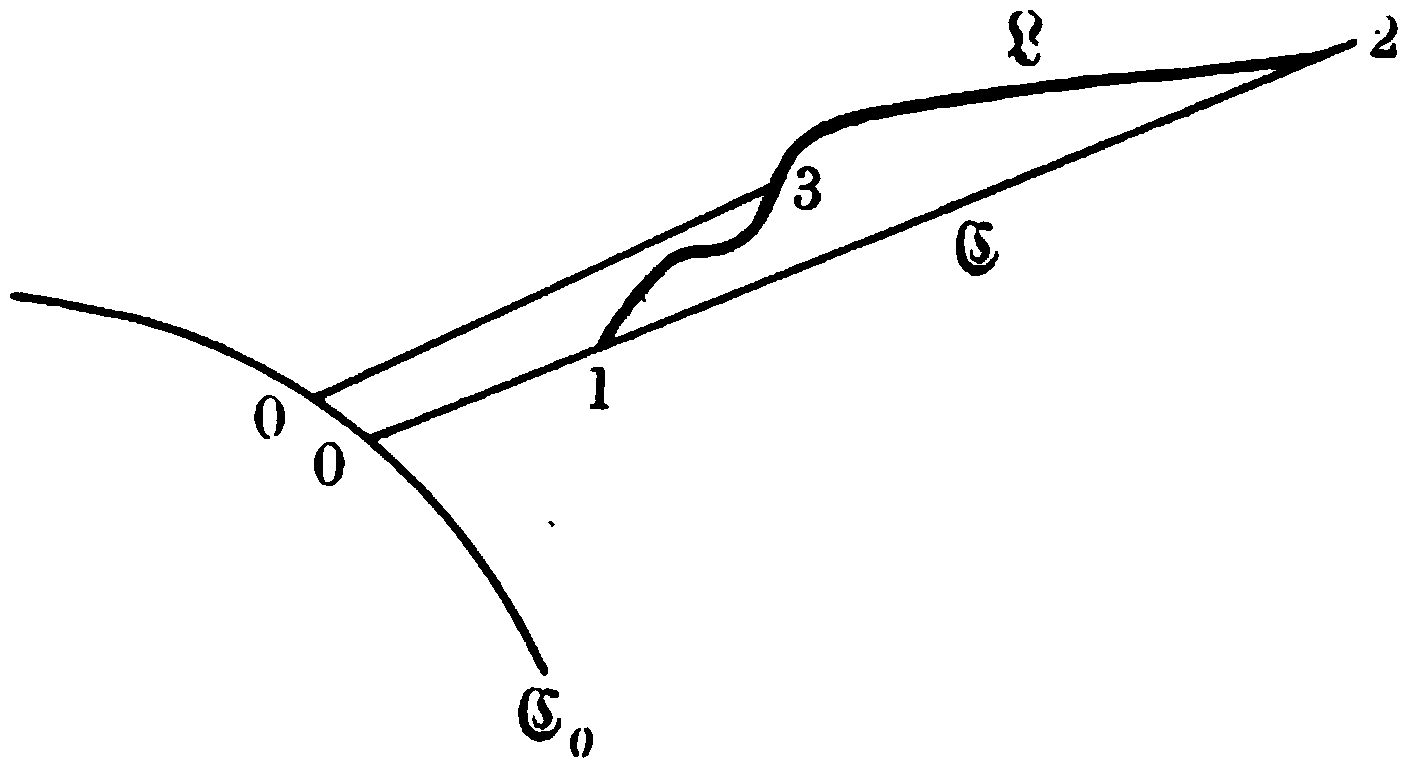
\includegraphics[width=\linewidth,height=32mm,keepaspectratio]{fig_assets/fig08_src_clean_x8.png}
\end{minipage}\hfill
\begin{minipage}[c]{0.49\linewidth}\centering
\end{minipage}
\end{center}

 Let the points 1 and 2 be joined by another curve $\Omega$ belonging to the field, along which the point 3 runs from 1 to 2. This curve is to have the properties of the curve so denoted in \S~17, so that $x_3,y_3$ are functions of a parameter $\tau$ belonging to the functions $\varphi(\tau)$ investigated there; the parameter $t$ increases in the direction from 1 toward 2. Through each position of the point 3 there then passes a definite extremal of the field, whose parameter $a$, as well as the argument $t$ corresponding on it to the point 3, are, by \S~14, regular functions of $x_3,y_3$. This extremal cuts out on the curve $\mathfrak{C}_0$ a point 0, whose coordinates, as well as its associated argument $t_0$, are, by \S~14, regular functions of $a$ and, with sufficient restriction of the field as well as of the curve-piece $\mathfrak{C}_0$, are uniquely determined. If, therefore, one sets
\[
\omega(a)=
F(\xi,\eta,\xi_t,\eta_t)\frac{dt_0}{da}
+F_{x'}(\xi,\ldots,\eta_t)\xi_a
+F_{y'}(\xi,\ldots,\eta_t)\eta_a\bigg|^0,
\]
then this expression is a regular function of $a$; if, again,
\[
u=\overline{J}_{03}
\]
% src-pdfpage=0097
% src-break=0097
is set, formula (31) gives
\[
\frac{\partial u}{\partial a}
=
\frac{\partial\overline{J}_{03}}{\partial a}
=
-\omega(a)+F_{x'}(\xi,\ldots,\eta_t)\xi_a
+F_{y'}(\xi,\ldots,\eta_t)\eta_a\bigg|^3,
\]
and if the point 3 is thought of as movable on a definite extremal 03, one obtains immediately
\[
\frac{\partial u}{\partial t}=F(\xi,\eta,\xi_t,\eta_t)\bigg|^3.
\]
Now $a,t$, as well as $x_3,y_3$, are functions of $\tau$ belonging to those denoted in \S~17 by $\varphi(\tau)$; hence, if each differentiation with respect to $\tau$ always refers to forward derivatives, the last two equations give
\[
\frac{d\overline{J}_{03}}{d\tau}
=
-\omega(a)\frac{da}{d\tau}
+F_{x'}(\xi,\ldots,\eta_t)\frac{dx}{d\tau}
+F_{y'}(\xi,\ldots,\eta_t)\frac{dy}{d\tau}\bigg|^3.
\]
Further, the integral $J_{32}$ formed along the curve $\Omega$, which as a function of $\tau$ likewise has the character of $\varphi(\tau)$, satisfies the equation
\[
\frac{dJ_{32}}{d\tau}
=
-F\left(x,y,\frac{dx}{d\tau},\frac{dy}{d\tau}\right)\bigg|^3;
\]
therefore, replacing $\xi_t,\eta_t$ by $x',y'$, one obtains
\[
\frac{d(\overline{J}_{03}+J_{32})}{d\tau}
=
-\omega(a)\frac{da}{d\tau}
+F_{x'}(x,y,x',y')\frac{dx}{d\tau}
\]
\[
\qquad
+F_{y'}(x,y,x',y')\frac{dy}{d\tau}
-F\left(x,y,\frac{dx}{d\tau},\frac{dy}{d\tau}\right).
\]
Let the sum of the last three terms be called $\mathfrak{E}$, or more exactly
\[
\mathfrak{E}\left(x,y,x',y',\frac{dx}{d\tau},\frac{dy}{d\tau}\right).
\]
If now the point 3 lies specially in its initial position 1 and its final position 2, then the corresponding values of the sum $\overline{J}_{03}+J_{32}$ are
\[
\overline{J}_{01}+J_{12},\quad
\overline{J}_{02}=\overline{J}_{01}+\overline{J}_{12},
\]
and hence for the difference of the two it follows that
\[
\overline{J}_{12}-J_{12}
=
\int_{\tau_1}^{\tau_2}
\frac{d(\overline{J}_{03}+J_{32})}{d\tau}\,d\tau
=
-\int_{\tau_1}^{\tau_2}\omega(a)\frac{da}{d\tau}\,d\tau
+\int_{\tau_1}^{\tau_2}\mathfrak{E}\,d\tau.
\]
But the first summand on the right vanishes; for if one sets
\[
\int \omega(a)\,da=\xi(a),
\]
% src-pdfpage=0098
% src-break=0098
then $\xi$ is likewise a function regular for $a=a_0$, and one has
\[
\int_{\tau_1}^{\tau_2}\omega(a)\frac{da}{d\tau}\,d\tau
=
\int_{\tau_1}^{\tau_2}\frac{d\xi(a)}{d\tau}\,d\tau
=
\xi(a)\bigg|_1^2;
\]
but this quantity has the value 0, since $a$ has the same value $a_0$ at the points 1 and 2. Thus it follows that
\begin{equation}\tag{54}
\overline{J}_{12}-J_{12}
=
-\int_{\tau_1}^{\tau_2}
\mathfrak{E}\left(x,y,x',y',\frac{dx}{d\tau},\frac{dy}{d\tau}\right)d\tau,
\end{equation}
and the left-hand side has a fixed sign if the same is true of $\mathfrak{E}$.

If, in the case where all extremals of the field pass through the point 0, one wishes to test precisely the extremal arc 02, then one replaces only the curve $\mathfrak{C}_0$ by the fixed point 0; the formula
\begin{equation}\tag{55}
d\overline{J}_{03}=du=F_{x'}\,dx+F_{y'}\,dy,
\end{equation}
which, if necessary, must have been proved by special considerations, immediately gives
\begin{equation}\tag{56}
\frac{d(\overline{J}_{03}+J_{32})}{d\tau}=\mathfrak{E},\quad
J_{02}-\overline{J}_{02}
=
-\int_{\tau_0}^{\tau_2}\mathfrak{E}\,d\tau,
\end{equation}
so long as the comparison curve $\Omega$ remains within the surface which the extremals issuing from the point 0 cover simply.

The simple formula (55) for $du$ remains valid, by \S~15, also when the curve $\mathfrak{C}_0$ is cut transversally by the extremals of the field (Fig.~9); then $\omega(a)$ vanishes identically.

% unit: fig9 source=kneser_lvr_1900_archiveorg.pdf#p0098 authorial=true type=hq_sourcecrop


\begin{center}
{\small Fig.~9.}\par\vspace{1mm}
\begin{minipage}[c]{0.47\linewidth}\centering
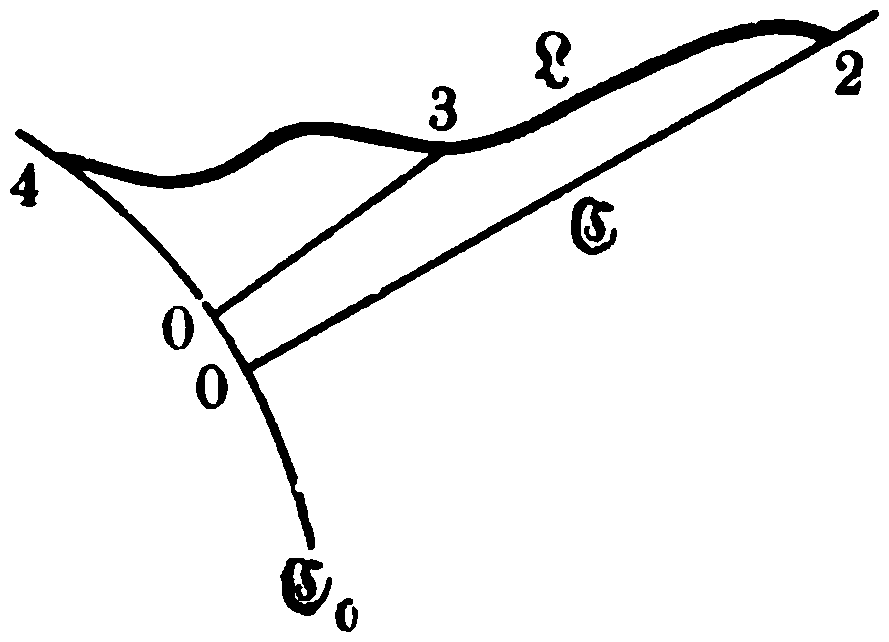
\includegraphics[width=\linewidth,height=32mm,keepaspectratio]{fig_assets/fig09_src_clean_x8.png}
\end{minipage}\hfill
\begin{minipage}[c]{0.49\linewidth}\centering
\end{minipage}
\end{center}

 We make use of this in order, by means of the expression $\mathfrak{E}$, to derive a criterion also for the extremum with one variable boundary. Let the point 4 lie on the curve $\mathfrak{C}_0$, and 2, as before, on the curve $\mathfrak{C}$; let both be joined by a curve $\Omega$ remaining in the field, which is traversed by the point 3 in the direction from 4 toward 2. Then the initial and final values of the sum $\overline{J}_{03}+J_{32}$ are the quantities
\[
J_{42},\quad \overline{J}_{02},
\]
% src-pdfpage=0099
% src-break=0099
and one has, as before,
\[
\frac{d\overline{J}_{03}}{d\tau}
=
F_{x'}\frac{dx}{d\tau}
+F_{y'}\frac{dy}{d\tau},
\quad
\frac{dJ_{32}}{d\tau}
=
-F\left(x,y,\frac{dx}{d\tau},\frac{dy}{d\tau}\right),
\]
therefore
\begin{equation}\tag{57}
J_{42}-\overline{J}_{02}
=
-\int_{\tau_4}^{\tau_2}\mathfrak{E}\,d\tau.
\end{equation}





\begin{center}{\large \S~21.}\end{center}

The quantity $\mathfrak{E}$, by whose investigation the question of the occurrence of the extremum can now be decided, plainly depends on the point 2 $(x,y)$ and on the two line-elements issuing from it, which are determined on the extremal of the field and on the curve $\Omega$ by the sense of increasing parameters $t$ and $\tau$. If both quantities $x'$ and $\dfrac{dx}{d\tau}$ are different from zero, so that one can set
\[
D x=\frac{dx}{d\tau}\,d\tau,\quad
D y=\frac{dy}{d\tau}\,d\tau=\bar{p}\,D x,\quad
dy=p\,dx,
\]
\[
F(x,y,x',y')dt=f(x,y,p)dx,
\]
\[
F\left(x,y,\frac{dx}{d\tau},\frac{dy}{d\tau}\right)d\tau
=
f(x,y,\bar{p})D x,
\]
then one obtains
\begin{equation}\tag{58}
\mathfrak{E}\,d\tau
=
\{f(x,y,p)+(\bar{p}-p)f_p(x,y,p)-f(x,y,\bar{p})\}D x.
\end{equation}
To be sure, the quantities $x'$ and $y'$ characterising the first line-element occur only in $F_{x'}$ and $F_{y'}$, expressions which depend only on $x':y'$. From this, however, it cannot be concluded that $\mathfrak{E}$ keeps the same value when one replaces the element of the extremal by its opposite; for even if $F$ is a single-valued function of $x'$ and $y'$, still (\S~3) $F_{x'}$ and $F_{y'}$ need not be single-valued functions of $x':y'$. The quantities
\[
\mathfrak{E}\left(x,y,x',y',\frac{dx}{d\tau},\frac{dy}{d\tau}\right),\quad
\mathfrak{E}\left(x,y,-x',-y',\frac{dx}{d\tau},\frac{dy}{d\tau}\right)
\]
therefore need not be equal, and just as little need the quantities
\[
\mathfrak{E}\left(x,y,x',y',\frac{dx}{d\tau},\frac{dy}{d\tau}\right),\quad
\mathfrak{E}\left(x,y,x',y',-\frac{dx}{d\tau},-\frac{dy}{d\tau}\right)
\]
be opposite to one another (examples below).

% src-pdfpage=0100
% src-break=0100
The two line-elements on which $\mathfrak{E}$ depends coincide then and only then when there exists a positive quantity $\alpha$ satisfying the equations
\begin{equation}\tag{59}
x'=\alpha\frac{dx}{d\tau},\quad
y'=\alpha\frac{dy}{d\tau}
\end{equation}
In this case one has
\[
F_{x'}(x,y,x',y')
=
F_{x'}\left(x,y,\frac{dx}{d\tau},\frac{dy}{d\tau}\right),
\]
\[
F_{y'}(x,y,x',y')
=
F_{y'}\left(x,y,\frac{dx}{d\tau},\frac{dy}{d\tau}\right);
\]
since now always
\[
\frac{dx}{d\tau}F_{x'}\left(x,y,\frac{dx}{d\tau},\frac{dy}{d\tau}\right)
\]
\[
+
\frac{dy}{d\tau}F_{y'}\left(x,y,\frac{dx}{d\tau},\frac{dy}{d\tau}\right)
-
F\left(x,y,\frac{dx}{d\tau},\frac{dy}{d\tau}\right)=0,
\]
it follows that
\[
\mathfrak{E}=0.
\]
We then say that $\mathfrak{E}$ vanishes in an ordinary manner. If $\mathfrak{E}$ takes the value zero without the equations (59) holding with a positive value $\alpha$, we call the vanishing extraordinary.

Geometrically, the meaning of the quantity $\mathfrak{E}$ can be characterised if we anticipate what we shall prove later (\S~30), though otherwise we do not use it now, namely that every sufficiently small piece of an extremal can in general be surrounded by a field. Let 78 and 79 be the line-elements (Fig.~10) which belong to the systems of values $(x,y,dx,dy)$, $(x,y,Dx,Dy)$;

% unit: fig10 source=kneser_lvr_1900_archiveorg.pdf#p0100 authorial=true type=hq_sourcecrop


\begin{center}
{\small Fig.~10.}\par\vspace{1mm}
\begin{minipage}[c]{0.47\linewidth}\centering
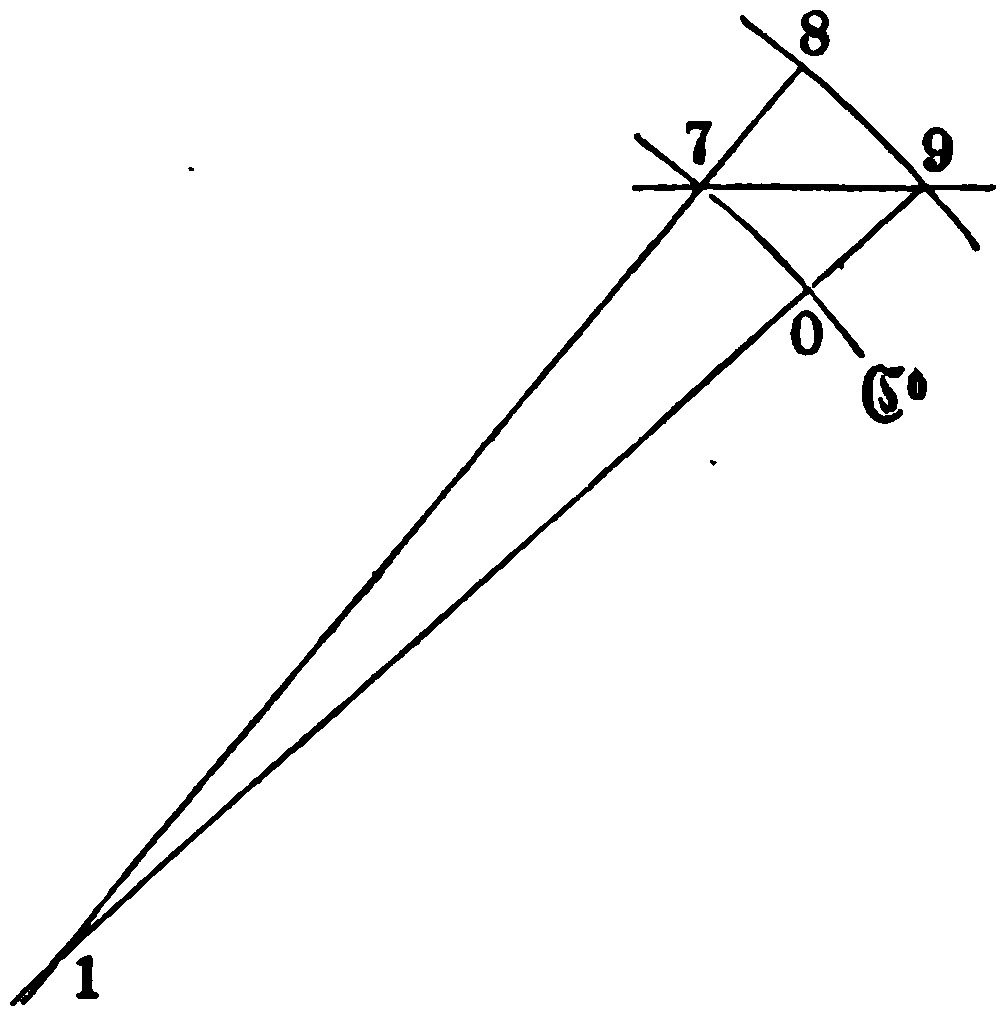
\includegraphics[width=\linewidth,height=32mm,keepaspectratio]{fig_assets/fig10_src_clean_x8.png}
\end{minipage}\hfill
\begin{minipage}[c]{0.49\linewidth}\centering
\end{minipage}
\end{center}

 then draw an extremal in the direction 78, and surround it near the point 7 with a field whose extremals may cut transversally the curve $\mathfrak{C}^0$ passing through the point 7, as well as a curve 89. Let the former be cut at the point 0 by the extremal of the field passing through 9; then $\overline{J}_{09}$ or $\overline{J}_{78}$ can be regarded as the differential, reckoned from the curve $\mathfrak{C}^0$, of the quantity $u$ in the sense of
% src-pdfpage=0101
% src-break=0101
\S~15, and one has, by formula (34),
\[
\overline{J}_{09}=\overline{J}_{78}
=
F_{x'}(x,y,dx,dy)D x+F_{y'}(x,y,dx,dy)D y.
\]
If the extremals 78 and 09 intersect in a point 1 which, from 7, lies on the side opposite to 8, then by \S~15
\[
\overline{J}_{17}=\overline{J}_{10},\quad
\mathfrak{E}\,d\tau
=
\overline{J}_{78}-J_{79}
=
\overline{J}_{19}-\overline{J}_{17}-J_{79}.
\]
From this one sees that the quantity $\mathfrak{E}d\tau$ is independent of the coordinate system, which is also evident from the identity developed in \S~16,
\[
F_{x'}(x,y,dx,dy)D x+F_{y'}(x,y,dx,dy)D y
\]
\[
=
G_{u'}(u,v,du,dv)D u+G_{v'}(u,v,du,dv)D v.
\]

In particular, one may therefore imagine the coordinate system rotated so that for the two elements 78 and 79 the differential $dx$ has the same sign, that is, so that both elements point to the same side of a parallel to the $y$-axis. Then
\[
p=\frac{dy}{dx},\quad
\bar{p}=\frac{dy}{d\tau}:\frac{dx}{d\tau}=D y:D x
\]
are finite quantities, and the elements are defined by the systems of values $(x,y,p,dx)$, $(x,y,\bar{p},dx)$. If now $F$ is regular for all arc-elements issuing from the point $(x,y)$, then by \S~5 the same holds for
\[
f(x,y,p)=\frac{F}{x'}
\]
for all elements which fall in the concave angle formed by the directions 78 and 79, since for them $x'$ is different from zero; thus $f$ is regular for the interval from $p$ to $\bar{p}$, and, if $\theta$ is a proper fraction, one can set, according to (58),
\[
f(x,y,\bar{p})=f(x,y,p)+(\bar{p}-p)f_p(x,y,p)
+\frac{1}{2}(\bar{p}-p)^2 f_{pp}[x,y,p+\theta(\bar{p}-p)],
\]
\begin{equation}\tag{60}
\mathfrak{E}d\tau
=
-\frac{1}{2}(\bar{p}-p)^2 f_{pp}[x,y,p+\theta(\bar{p}-p)]\,dx.
\end{equation}
The quantity $\mathfrak{E}$ has the fixed sign of $-F_1$ and vanishes only in an ordinary manner if Legendre's condition for the strong extremum is satisfied; for the product
\[
f_{pp}[x,y,p+\theta(\bar{p}-p)]\,dx
\]
is identical with the quantity $F_1(x,y,dx,dy)dx^4$, which belongs to the arc-element passing through the point $(x,y)$ and whose components
\[
dx,\ [p+\theta(\bar{p}-p)]dx=dy
\]
% src-pdfpage=0102
% src-break=0102
are as stated, and the assertion just made is thereby proved. If, however, only Legendre's condition for the weak extremum is assumed to be satisfied, then $\mathfrak{E}$ has the two indicated properties only so long as the two determining elements 78, 79 deviate sufficiently little in position and direction from an element of the curve $\mathfrak{C}$ taken in the direction of integration. Conversely, one cannot in the same way infer from the sign of the quantity $\mathfrak{E}$ the sign of the quantity $F_1$.



\begin{center}{\large \S~22.}\end{center}

In general, if $t$ and $a$ refer to the point 3 which traverses the curve $\Omega$, one has
\[
x=\xi(t,a),\quad y=\eta(t,a),
\]
\[
\frac{dx}{d\tau}=\xi_t\frac{dt}{d\tau}+\xi_a\frac{da}{d\tau},\quad
\frac{dy}{d\tau}=\eta_t\frac{dt}{d\tau}+\eta_a\frac{da}{d\tau},
\]
\[
x'=\xi_t,\quad y'=\eta_t.
\]
If now along the whole curve $\Omega$ the quantity $\mathfrak{E}$ were to vanish ordinarily at all points, the equations (59) would result, and with them
\[
\begin{vmatrix}
x' & \dfrac{dx}{d\tau}\\[0.7em]
y' & \dfrac{dy}{d\tau}
\end{vmatrix}
=
\begin{vmatrix}
\xi_t & \xi_a\dfrac{da}{d\tau}\\[0.7em]
\eta_t & \eta_a\dfrac{da}{d\tau}
\end{vmatrix}
=
\Delta\frac{da}{d\tau}=0.
\]
Since $\Delta$ is different from zero, it follows for a finite interval of the argument $\tau$ that
\[
\frac{da}{d\tau}=0.
\]
From this, since $a$ as a function of $\tau$ has the properties of the function $\varphi(\tau)$ defined in \S~17, it follows that $a$ must be constant along the whole curve $\Omega$ and equal to its initial value $a_0$.

Thus, if the curve $\Omega$ does not completely coincide with $\mathfrak{C}$, if further an extraordinary vanishing of the quantity $\mathfrak{E}$ is excluded either altogether or by restrictions on the curves $\Omega$, and if no change of sign takes place in the ordinary vanishing along the curve $\Omega$, then the right-hand sides of equations (54), (56), (57) in \S~20 are different from zero and
% src-pdfpage=0103
% src-break=0103
of fixed sign. The extremals 12, 02 therefore in fact yield an extremum of the integral $J$ in comparison with curves $\Omega$ restricted in the indicated way, namely a maximum or minimum according as $\mathfrak{E}$ is positive or negative.

In particular, if the curve $\Omega$ lies in a narrower neighbourhood, defined by $\rho$ and $\rho_1$ according to \S~17, of the arc 12 of the curve $\mathfrak{C}$, then the angle made by a tangent drawn in the sense of increasing $t$ to the latter with a similar tangent to an extremal of the field whose point of contact is less than $\rho$ distant from that of the former lies below a bound $\rho_2$, which decreases without bound with $\rho$. Now to every tangent of the curve $\Omega$ there is a corresponding tangent of the arc 12 whose point of contact is also less than $\rho$ from its own and which forms with it an angle not exceeding $\rho_1$; the angle of the tangent of the curve $\Omega$ with the extremal passing through its point of contact is therefore less than $\rho_1+\rho_2$ and, with sufficient limitation of the neighbourhood, becomes arbitrarily small. In order to secure the weak extremum, it is therefore enough that $\mathfrak{E}$ have a fixed sign only for the case in which the two line-elements determining its value are inclined arbitrarily little to one another and to an element of the curve $\mathfrak{C}$ taken in the direction of integration, and vanish only in an ordinary manner. In case a) of \S~17 this stipulation may take the place of the one relating to $F_1$, from which it follows by \S~21.

Further, in order to be able to infer the strong extremum from equations (54), (56), (57) of \S~20, first the integrand must be regular for arbitrarily directed line-elements of the field, and secondly the quantity $\mathfrak{E}(x,y,x',y',D x,D y)$ must have the properties indicated above when $(D x,D y)$ is any line-element issuing from the point $(x,y)$, while $x',y'$ refer to the extremal of the field passing through this point. In the criteria for the strong extremum set up earlier (\S~17), Legendre's condition in case b) may therefore be replaced by the less demanding Weierstrass condition that the quantity $\mathfrak{E}(x,y,x',y',D x,D y)$ possess a fixed sign at all points of a certain region embracing the arc 02 and vanish only when the line-elements $(x',y')$ and $(D x,D y)$ coincide.

In both cases a) and b), moreover, the requirement used essentially in \S\S~16 and 17,
% src-pdfpage=0104
% src-break=0104
that the integrand $F$ not vanish, can be dropped, since the present development is evidently independent of this assumption.

\begin{center}{\large \S~23.}\end{center}

\noindent\textbf{Examples. Problem I (\S~9).} Here one sets, with positive square root,
\[
F=\sqrt{x'^2+y'^2},
\]
\[
\mathfrak{E}
=
\frac{x'}{\sqrt{x'^2+y'^2}}\frac{dx}{d\tau}
+
\frac{y'}{\sqrt{x'^2+y'^2}}\frac{dy}{d\tau}
-
\sqrt{\left(\frac{dx}{d\tau}\right)^2+\left(\frac{dy}{d\tau}\right)^2}
\]
\[
=
\sqrt{\left(\frac{dx}{d\tau}\right)^2+\left(\frac{dy}{d\tau}\right)^2}
\{\cos(ds,Ds)-1\},
\]
where $ds,Ds$ are the arc-elements corresponding to the positive differentials $dt,d\tau$. The quantity $\mathfrak{E}$ is therefore never positive, and vanishes only when $ds$ and $Ds$ coincide. Formula (58) of \S~21 gives the same result if one sets
\[
Fdt=\sqrt{1+p^2}\,dx,\quad
F\left(x,y,\frac{dx}{d\tau},\frac{dy}{d\tau}\right)d\tau
=
\sqrt{1+\bar{p}^2}\,D x,
\]
where the square roots must have the sign of the differential standing beside them; one obtains
\[
\mathfrak{E}d\tau
=
\left\{\sqrt{1+p^2}+\frac{(\bar{p}-p)p}{\sqrt{1+p^2}}-\sqrt{1+\bar{p}^2}\right\}D x
\]
\[
=
\sqrt{1+\bar{p}^2}\,D x
\left\{\frac{\bar{p}p+1}{\sqrt{1+p^2}\sqrt{1+\bar{p}^2}}-1\right\},
\]
and this expression, too, is never positive, since
\[
\sqrt{1+\bar{p}^2}\,D x
\]
is positive, while the adjacent bracket is negative or zero in consequence of the inequality
\[
(1+p\bar{p})^2\leq (1+p^2)(1+\bar{p}^2).
\]
Geometrically this result means, according to \S~21, that in a triangle 179, in which the side 79 is small in relation to the others, the inequality
\begin{equation}\tag{61}
\overline{J}_{19}-\overline{J}_{17}-J_{79}<0
\end{equation}
holds, that is, the sum of the sides 17, 79 is greater than 19. The proof, carried out by means of the expression $\mathfrak{E}$, for the occurrence of the
% src-pdfpage=0105
% src-break=0105
extremum admits in this problem a wholly elementary geometrical interpretation. If 145 are three points (Fig.~11) of a straight line, and 7, 9 two positions of the point 2, which traverses any curve 45 from 4 toward 5,

% unit: fig11 source=kneser_lvr_1900_archiveorg.pdf#p0105 authorial=true type=hq_sourcecrop


\pagebreak[4]

\begin{center}
{\small Fig.~11.}\par\vspace{1mm}
\begin{minipage}[c]{0.47\linewidth}\centering
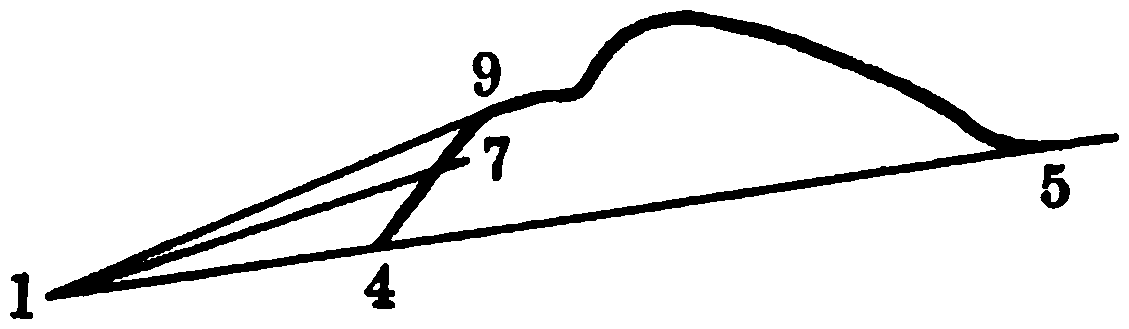
\includegraphics[width=\linewidth,height=32mm,keepaspectratio]{fig_assets/fig11_src_clean_x8.png}
\end{minipage}\hfill
\begin{minipage}[c]{0.49\linewidth}\centering
\end{minipage}
\end{center}

 then by (61), denoting lengths of straight segments by $\overline{J}$, one has
\[
\overline{J}_{17}+J_{75}>\overline{J}_{19}+J_{95},
\]
and so the quantity $J_{13}+J_{23}$ decreases, and at the beginning has a greater value than at the end of the motion of the point 2.



\noindent\textbf{Problem II (\S~9).} The quantity $\mathfrak{E}$ differs from the one obtained for Problem I only by the positive factor $y$, and so Weierstrass' condition for the strong minimum is satisfied.

We introduce the hyperbolic functions and set
\[
\Cof z=\frac{e^z+e^{-z}}{2},\quad
\Sin z=\frac{e^z-e^{-z}}{2},\quad
\Tg z=\frac{1}{\Ctg z}=\frac{\Sin z}{\Cof z},
\]
where the equations
\[
\Cof^2z-\Sin^2z=1,\quad
d\Cof z=\Sin z\,dz,\quad
d\Sin z=\Cof z\,dz,
\]
\[
d\Tg z=\frac{dz}{\Cof^2z},\quad
d\Ctg z=\frac{-dz}{\Sin^2z}
\]
hold; then for the extremals the equations
\begin{equation}\tag{62}
y=a\Cof\frac{x-b}{a},\quad
p=\Sin\frac{x-b}{a}.
\end{equation}
hold. We consider in particular those extremals which cut the given curve $\mathfrak{C}_0$ transversally, that is, orthogonally (\S~11). Let the equation of this curve be
\[
y_0=f(x_0);
\]
then the constants of the orthogonally cutting extremals are subject to the equations
\[
y_0=a\Cof\frac{x_0-b}{a},\quad
1+p_0f'(x_0)=0
\]
or, if
\[
u=\frac{x-b}{a},\quad u_0=\frac{x_0-b}{a}
\]
is set,
% src-pdfpage=0106
% src-break=0106
\begin{equation}\tag{63}
f(x_0)=a\Cof u_0,\quad
1+f'(x_0)\Sin u_0=0.
\end{equation}
Differentiating here, and in the first equation (62), with respect to $x,x_0,a,b$, gives
\[
dy=\Sin u\,dx+0\,dx_0+(\Cof u-u\Sin u)\,da-\Sin u\,db,
\]
\[
0=[\Sin u_0-f'(x_0)]\,dx_0+(\Cof u_0-u_0\Sin u_0)\,da-\Sin u_0\,db,
\]
\begin{equation}\tag{64}
0=
\left[\frac{f'(x_0)}{a}\Cof u_0+f''(x_0)\Sin u_0\right]dx_0
-\frac{f'(x_0)}{a}u_0\Cof u_0\,da
-\frac{f'(x_0)}{a}\Cof u_0\,db.
\end{equation}
The determinant of the terms affected by $da,db$ in the last two equations is
\[
M=
\frac{f'(x_0)\Cof u_0}{a}
\begin{vmatrix}
\Cof u_0-u_0\Sin u_0 & -\Sin u_0\\
-u_0 & -1
\end{vmatrix}
=
\frac{f'(x_0)\Cof^2u_0}{-a},
\]
and is therefore different from zero if, as we shall assume, the curve $\mathfrak{C}_0$ at the point under consideration does not run parallel to the $x$-axis. One may therefore think of $a$ and $b$ as regular functions of $x_0$ determined from the equations (63), and obtains $y$ expressed by $x$ and $x_0$. Since, further, along every catenary $y$ is a single-valued function of $x$, one may set $t=x$; for the family of extremals which cuts $\mathfrak{C}_0$ orthogonally one therefore obtains
\[
\Delta=\frac{\partial(x,y)}{\partial(x,x_0)}=\frac{\partial y}{\partial x_0},\quad
dy=p\,dx+\Delta\,dx_0.
\]
From the equations (64), however, eliminating $da$ and $db$ by an elementary calculation, one obtains
\[
M\,dy=M\Sin u\,dx+dx_0(\ldots),
\]
where the factor of $dx_0$ is the determinant of the coefficients of $dx_0,da,db$ in the cited equations; hence
\[
M\Delta=
\begin{vmatrix}
0 & \Cof u-u\Sin u & -\Sin u\\
\Sin u_0-f'(x_0) & \Cof u_0-u_0\Sin u_0 & -\Sin u_0\\
\dfrac{f'(x_0)}{a}\Cof u_0+f''(x_0)\Sin u_0 &
-\dfrac{f'(x_0)}{a}u_0\Cof u_0 &
-\dfrac{f'(x_0)}{a}\Cof u_0
\end{vmatrix}.
\]
So long as this expression does not vanish, the extremal arc 02 cutting the line $\mathfrak{C}_0$ orthogonally at the point 0 supplies a strong minimum of the surface of revolution, compared with all curves which join $\mathfrak{C}_0$ to the point 2.

If one further takes account of the second equation (63) and sets
% src-pdfpage=0107
% src-break=0107
\[
\frac{f''(x_0)}{\left(\sqrt{1+[f'(x_0)]^2}\right)^3}
=
\frac{f''(x_0)}{(1+\Sin^{-2}u_0)^{3/2}}
=
f''(x_0)\Tg^3u_0
=
\frac{1}{r},
\]
then $|r|$ is the radius of curvature of the curve $\mathfrak{C}_0$, and one can write
\[
M\Delta
=
-\frac{\Cof^3u_0}{r\Sin^2u_0}
\begin{vmatrix}
\Cof u-u\Sin u & \Sin u\\
\Cof u_0-u_0\Sin u_0 & \Sin u_0
\end{vmatrix}
\]
\[
\qquad
+\frac{\Cof^2u_0}{y_0\Sin u_0}
\begin{vmatrix}
0 & \Cof u-u\Sin u & -\Sin u\\
\Cof u_0\Ctg u_0 & \Cof u_0-u_0\Sin u_0 & -\Sin u_0\\
-1 & u_0 & 1
\end{vmatrix}.
\]
If $\mathfrak{C}_0$ passes into an infinitely small circle, then $r=0$, and the equation $\Delta=0$ requires
\[
\begin{vmatrix}
\Cof u-u\Sin u & \Sin u\\
\Cof u_0-u_0\Sin u_0 & \Sin u_0
\end{vmatrix}
=0,\quad
\Ctg u-u=\Ctg u_0-u_0
\]
or
\[
\frac{y}{p}-x=\frac{y_0}{p_0}-x_0;
\]
this equation expresses that the tangents of the extremal at the points 0 and $(x,y)$ meet on the $x$-axis. So long as this therefore does not occur for any two tangents of the arc 02, the extremals passing through the point 0 form a field of every arc 12 that is a part of 02. Since the points 0 and 1 may approach one another arbitrarily closely, it follows that every arc of the extremal of which no two tangents meet on the $x$-axis gives an extremum with fixed endpoints.

In the general case of a finite curvature of the curve $\mathfrak{C}_0$, the equation $\Delta=0$ has the form
\[
A(\Cof u-u\Sin u)+B\Sin u=0,
\]
where $A$ and $B$ depend only on $u_0,y_0$ and $1:r$, and are linear with respect to the last quantity. If $A$ is different from zero, then one can write the equation
\begin{equation}\tag{65}
\Ctg u-u+\frac{B}{A}=0;
\end{equation}
the left-hand side then has the derivative
\[
-\frac{1}{\Sin^2u}-1,
\]
and therefore steadily decreases for increasing values of $u$. Now one easily finds
% src-pdfpage=0108
% src-break=0108
\[
\Ctg(\mp\infty)=\mp1,\quad \Ctg(\pm0)=\pm\infty,
\]
so equation (65) has a single finite root if
\[
|B|>|A|,
\]
and otherwise it has no root. If, further, one fixes $u_0$ and $y_0$, that is, holds fixed the point 0 and the direction of the curve $\mathfrak{C}_0$, then the curvature of this curve can be so chosen that $B:A$ obtains a prescribed value; one can therefore, by a suitable choice of $r$, always arrange that the extremal perpendicular to the curve $\mathfrak{C}_0$ ceases at a prescribed point 2 to furnish with certainty a minimum in comparison with the curves joining $\mathfrak{C}_0$ to the point 2.

\noindent\textbf{Problem IV (\S~9).} Let $\Omega$ be any line in the $wy$-plane which, from the point $w=y=0$, passes through the half-plane $y>0$ and descends again to the line $y$, with the continuity properties of the line so denoted in \S~17, and let the parameter $\tau$ have the value $\tau_0$ at the origin of coordinates. Then, putting $w$ for the symbol $u$ of \S~9, one has
\begin{equation}\tag{66}
x=\int_{\tau_0}^{\tau}
y\sqrt{\left(\frac{dw}{d\tau}\right)^2+\left(\frac{dy}{d\tau}\right)^2}\,d\tau
\end{equation}
with positive square root, and hence certainly
\begin{equation}\tag{67}
x\geq \int_{\tau_0}^{\tau}y\frac{dy}{d\tau}\,d\tau,\quad
x\geq \frac{y^2}{2}.
\end{equation}
Equality holds only when between $\tau_0$ and $\tau$ one always has
\[
\frac{dw}{d\tau}=0.
\]
The corresponding curve $\Omega_1$ in the $xy$-plane therefore lies in the first quadrant $(x>0,y>0)$ and in the interior, that is, on the concave side of the parabola
\begin{equation}\tag{68}
y^2=2x.
\end{equation}
The interior of this parabola is covered exactly simply by the extremals issuing from the point $0(x=y=0)$,
\begin{equation}\tag{69}
1-\frac{x}{a^2}
=
\sqrt{1-\left(\frac{y}{a}\right)^2},\quad
\frac{x^2}{a^2}=2x-y^2,
\end{equation}
since from these equations there results a single positive value of $a^2$ when $x,y$ are given and
% src-pdfpage=0109
% src-break=0109
$2x-y^2$ is positive. If the curve $\Omega$ first goes a certain distance parallel to the $y$-axis, then the curve $\Omega_1$ has a corresponding piece 01 in common with the parabola (68), which contributes zero to $J$; hence, if 3 is the endpoint of the curve $\Omega_1$, and therefore $y_3=0$, then along it one has
\begin{equation}\tag{70}
J_{03}=J_{13}.
\end{equation}
If the curve $\Omega_1$ has once left the parabola, it cannot reach it again, since then $dw:d\tau$ is different from zero at least along some piece, and in relation (67) the equality sign can therefore no longer hold.

The ellipses (69) form a field inside that half of the parabola (68) for which $y>0$; for here
\[
x=\xi=t,\quad
y=\eta=\sqrt{2t-\left(\frac{t}{a}\right)^2},
\]
from which one obtains
\[
\Delta=\frac{\partial(\xi,\eta)}{\partial(t,a)}
=\frac{\partial y}{\partial a}
=
\frac{t^2}{a^3}\left(2t-\frac{t^2}{a^2}\right)^{-1/2},
\]
a value which is plainly different from zero. One further finds, when $a$ and the square root are positive and 2 is any point of the region considered:
\begin{equation}\tag{71}
u=\overline{J}_{02}
=
\int_0^x y\sqrt{1-y^2p^2}\,dx
=
\int_0^x\frac{y^2}{a}\,dx
=
\frac{x^2}{a}-\frac{x^3}{3a^3}
\end{equation}
and easily verifies, expressing $dy$ by means of equation (69) through $dx$ and $da$, and referring $x',y',p$ to the extremals of the field, the equations
\[
F_{x'}=a,\quad F_{y'}=-ay^2p,\quad du=F_{x'}dx+F_{y'}dy;
\]
from this it follows, when the point 2 runs along the curve $\Omega_1$ from 1 to 3, that
\[
d(\overline{J}_{02}+J_{23})=\mathfrak{E}\,d\tau,
\]
and by formula (58), when $D x$ and $\bar{p}$ refer to the line $\Omega_1$ and $p$ to the extremal, one has
\[
\mathfrak{E}d\tau
=
y\left\{
\frac{1-y^2p\bar{p}}{\sqrt{1-y^2p^2}}
-
\sqrt{1-y^2\bar{p}^2}
\right\}D x,
\]
where the square root in the denominator is positive. Now, for every direction under consideration, the quantity
% src-pdfpage=0110
% src-break=0110
\[
y\frac{dy}{dx}
=
\frac{dy}{\sqrt{dy^2+dw^2}}
\]
lies between the bounds $\pm1$ and attains these, even on the extremal of the field, only for $y=0$; so long, therefore, as $y$ does not vanish, $y^2p\bar{p}$ is a proper fraction and the quantity $1-y^2p\bar{p}$ positive. Since $y$ and $D x$ are positive, the same plainly holds for $\mathfrak{E}d\tau$ when $\sqrt{1-y^2\bar{p}^2}$ is negative; if this quantity has a positive value, then it follows from the general inequality
\[
(1-\alpha\beta)^2\geq(1-\alpha^2)(1-\beta^2),
\]
that $\mathfrak{E}d\tau$ is never negative and vanishes only when $p=\bar{p}$, that is, only in an ordinary manner, since the differential $dx$ referring to the extremal is positive just like $D x$. If the equation
\[
1-y^2\bar{p}^{\,2}=0,
\]
holds, then the integrand of the integral $J$ expressed in $x,y$ is indeed singular; but the original definition
\[
J=\int y^2\frac{dw}{d\tau}\,d\tau
=
\int y\sqrt{1-y^2\bar{p}^{\,2}}\frac{dx}{d\tau}\,d\tau
\]
shows that $J_{23}$ nevertheless remains a function $\varphi(\tau)$ in the sense of \S~17. The quantity $dJ_{23}$ vanishes in this case; $du$ has the expression
\[
du=a(1-y^2p\bar{p})\,dx,
\]
and so remains positive. Therefore, if $\mathfrak{E}$ does not vanish ordinarily everywhere on the curve $\Omega_1$, that is, if this curve does not coincide with one of the extremals (69), the quantity $\overline{J}_{02}+J_{23}$ steadily increases as long as the point 2 lies between 1 and 3; at these points themselves, of course, our considerations no longer hold. As the point 2 approaches the positions 1 and 3, that quantity converges to the limiting values $J_{13}$ and $\overline{J}_{03}$; for when the point 2 approaches a definite place of the parabola, formulas (69), (71) give
\[
\lim\frac{x}{a}=0,\quad \lim u=\lim\overline{J}_{02}=0.
\]
From the behavior of the quantity $\mathfrak{E}$ it therefore follows, taking relation (70) into account, if $\Omega_1$ is not one of the curves (69), that
% src-pdfpage=0111
% src-break=0111
\[
\overline{J}_{03}>J_{13},\quad
\overline{J}_{03}>J_{013},
\]
that is, the sphere has greater volume than the solid of the same surface area produced by rotation of the curve $\Omega$.

% src-pdfpage=0111 portion=lower
% unit: sec24 source=kneser_lvr_1900_archiveorg.pdf#p0111 authorial=true
\begin{center}{\large \S~24.}\end{center}

If one proceeds along the curve $\mathfrak{C}$ from the point 0 in the direction of increasing $t$, let 6 be the first point at which, after one has left 0, the quantity $\Delta$ vanishes. We assume that this occurs before the functions $\xi$ and $\eta$ lose their assumed properties along the curve $\mathfrak{C}$, so that 6 is still a regular point of this curve, in whose neighborhood a domain for the quantities $t,a$ is defined by the inequalities
\[
|t-t_6|<\varepsilon,\quad |a-a_0|<\varepsilon,
\]
within which the functions $\xi,\eta,F(\xi,\eta,\xi_t,\eta_t)$ remain regular and the quantity $\xi_t^2+\eta_t^2$ is different from zero. The corresponding points $(x,y)$, which are determined by the equations
\[
x=\xi(t,a),\quad y=\eta(t,a),
\]
no longer belong to the field of a part of the curve $\mathfrak{C}$, since in general they cover certain regions of the plane twice. If, as before, at the point 0 the curve $\mathfrak{C}_0$ has its beginning, and is cut transversally by the extremals of the field, then we call 6 the extremal focal point of the curve $\mathfrak{C}_0$ on the extremal $\mathfrak{C}$; if the curve $\mathfrak{C}_0$ contracts into the point 0, through which then also all extremals of the field pass, then 0 and 6 are called conjugate points, or more explicitly extremally conjugate points. For example, by \S~23, in Problem II conjugate points are characterized by the fact that their tangents cut one another on the $x$-axis; the extremal focal point of an arbitrary curve $\mathfrak{C}_0$ is defined by the easily discussable equation (65).

Important properties of the conjugate points and focal points rest on the fact that the quantity $\Delta$ satisfies a linear differential equation which is determined solely by the extremal $\mathfrak{C}$. The geometrical meaning of the quantity $\Delta$ leads to this equation, and is recognized from the following consideration. Let
% src-pdfpage=0112
% src-break=0112
\begin{equation}\tag{72}
\begin{aligned}
x&=\xi(t,a),\quad y=\eta(t,a),\\
\bar x&=\xi(t,a+\delta a),\quad \bar y=\eta(t,a+\delta a)
\end{aligned}
\end{equation}
be two neighboring extremals of the field, and let the point $(\bar x,\bar y)$ lie on the normal to the first curve at the point $(x,y)$. The direction cosines of this straight line are
\[
X=\frac{-y'}{\sqrt{x'^2+y'^2}},\quad Y=\frac{x'}{\sqrt{x'^2+y'^2}};
\]
if the square roots are taken positive, these quantities refer to that direction which is situated with respect to the direction of increasing $t$ as the $+y$-axis is situated with respect to the $+x$-axis. The equation of the normal is
\[
(\bar x-x)x'+(\bar y-y)y'=0;
\]
the equations (72) may be written
\[
\bar x-x-\{\xi_t(\tau-t)+\xi_a\delta a+[\tau-t,\delta a]_2\}=0,
\]
\[
\bar y-y-\{\eta_t(\tau-t)+\eta_a\delta a+[\tau-t,\delta a]_2\}=0,
\]
where the quantities $\xi_t,\xi_a\ldots$ are to be taken for the argument-system $t,a$. The functional determinant of the left sides of these three equations with respect to $\bar x,\bar y,\tau$ is, when $\bar x,\bar y,t$ is put for these,
\[
\begin{vmatrix}
x'&y'&0\\
1&0&-\xi_t\\
0&1&-\eta_t
\end{vmatrix}=x'^2+y'^2,
\]
and hence is different from zero; one may therefore expand the quantities $\bar x-x$, $\bar y-y$, $\tau-t$ according to $\delta a$, where the linear terms are the same as if the equations contained only those three differences strictly linearly; consequently it follows that
\[
\bar x-x=-\frac{\eta_t\Delta\delta a}{\xi_t^2+\eta_t^2}+[\delta a]_2,\quad
\bar y-y=\frac{\xi_t\Delta\delta a}{\xi_t^2+\eta_t^2}+[\delta a]_2,
\]
or, if
\begin{equation}\tag{73}
\omega=\frac{\Delta\delta a}{\sqrt{\xi_t^2+\eta_t^2}}
\end{equation}
is put,
\[
\bar x-x=X\omega+[\delta a]_2,
\quad
\bar y-y=Y\omega+[\delta a]_2;
\]
therefore $\omega$ is the normal distance of the two extremals when $\delta a$ becomes infinitely small, taken positively or negatively according as the direction toward the point $(\bar x,\bar y)$ agrees with the normal direction defined above or not.

% src-pdfpage=0113
% src-break=0113
Now the point $(\bar x,\bar y)$ defined by the equations (72), for an arbitrarily fixed value of $\delta a$, describes an extremal; if, as in \S~4, the equations of such an extremal are
\[
P=0,\quad Q=0,
\]
then one may substitute $\bar x,\bar y$ for $x,y$ in them and differentiate with respect to $\delta a$; if one then puts $\delta a=0$, the first equation, for example, gives
\[
\frac{\partial P}{\partial x}\frac{\partial\bar x}{\partial\delta a}
+\frac{\partial P}{\partial x'}\frac{\partial\bar x'}{\partial\delta a}
+\frac{\partial P}{\partial x''}\frac{\partial\bar x''}{\partial\delta a}
+\frac{\partial P}{\partial y}\frac{\partial\bar y}{\partial\delta a}+\cdots=0.
\]
This result may also be expressed in the following way: the equations
\[
\delta P=0,\quad \delta Q=0
\]
hold if one puts
\begin{equation}\tag{74}
\delta x=\omega X,
\quad
\delta y=\omega Y;
\end{equation}
these latter equations define what we shall call a normal variation. For evidently, apart from terms $[\delta a]_2$, the equations
\[
\delta a\frac{\partial\bar x}{\partial\delta a}=\omega X,
\quad
\delta a\frac{\partial\bar y}{\partial\delta a}=\omega Y
\]
hold, so that the operations
\[
\delta,
\quad \delta a\frac{\partial}{\partial\delta a}
\]
may be regarded as identical under the assumption (74). In order to carry out the calculations indicated, we start from the identities
\[
P=F_x-\frac{dF_{x'}}{dt},\quad
\delta P=\delta F_x-\frac{d\delta F_{x'}}{dt}
\]
and the latter gives easily
\[
\begin{aligned}
\delta P={}&\left(F_{xx}-\frac{dF_{xx'}}{dt}\right)\delta x
+\left(F_{xy}-\frac{dF_{x'y}}{dt}\right)\delta y\\
&-\frac{d}{dt}(F_{x'x'}\delta x'+F_{x'y'}\delta y')
+(F_{xy'}-F_{yx'})\delta y'
\end{aligned}
\]
and analogously one finds
\[
\begin{aligned}
\delta Q={}&\left(F_{yx}-\frac{dF_{xy'}}{dt}\right)\delta x
+\left(F_{yy}-\frac{dF_{yy'}}{dt}\right)\delta y\\
&-\frac{d}{dt}(F_{y'x'}\delta x'+F_{y'y'}\delta y')
+(F_{yx'}-F_{xy'})\delta x'.
\end{aligned}
\]
% src-pdfpage=0114
% src-break=0114
Now introduce the quantity $F_1$ defined in \S~16, and take into account that for the normal variation (74)
\[
y'\delta x'-x'\delta y'=-\omega'\sqrt{x'^2+y'^2};
\]
if one also puts
\[
F^1=F_1(x'^2+y'^2),
\]
\[
\begin{aligned}
F_2={}&\left(F_{xx}-\frac{dF_{xx'}}{dt}\right)X^2
+\left(2F_{xy}-\frac{dF_{x'y}}{dt}-\frac{dF_{y'x}}{dt}\right)XY\\
&+\left(F_{yy}-\frac{dF_{yy'}}{dt}\right)Y^2
+(F_{xy'}-F_{yx'})(XY'-YX'),
\end{aligned}
\]
then from the written-down values of $\delta P$ and $\delta Q$ there results
\[
X\delta P+Y\delta Q
=F_2\omega-X\frac{d}{dt}(F^1X\omega')-Y\frac{d}{dt}(F^1Y\omega');
\]
using the identities
\[
X^2+Y^2=1,
\quad
XX'+YY'=0
\]
it follows from this that
\begin{equation}\tag{75}
X\delta P+Y\delta Q=F_2\omega-\frac{d}{dt}\left(F^1\frac{d\omega}{dt}\right),
\end{equation}
and this, which we shall use later, is a pure identity under the assumption (74) and for arbitrary values of $\omega$.

If for $\omega$ one takes the value (73), then
\[
X\delta P+Y\delta Q=0,
\quad
F_2\omega-\frac{d}{dt}\left(F^1\frac{d\omega}{dt}\right)=0
\]
results. If therefore along the piece of the extremal under consideration
\[
x=\xi(t,a),\quad y=\eta(t,a),
\]
say along the arc 06, the quantity $F_1$ is different from zero, then $\omega$ satisfies a linear differential equation whose coefficients, if it is written in the form
\[
\omega''+M\omega'+N\omega=0,
\]
are regular functions of $t$ from $t_0$ to $t_6$. The quantity $\omega$ therefore, if it does not vanish identically, cannot vanish simultaneously with its derivative with respect to $t$, and according to equation (73) the same is true of $\Delta$, so that in any event
\[
\Delta_t(t_6,a_0)\gtrless0.
\]

% src-pdfpage=0115
% src-break=0115
% unit: sec25 source=kneser_lvr_1900_archiveorg.pdf#p0115 authorial=true
\begin{center}{\large \S~25.}\end{center}

The inequality obtained shows that one can solve the equation
\begin{equation}\tag{76}
\Delta(t,a)=0,
\end{equation}
which is satisfied by the value-system $t_6,a_0$, in a neighborhood of this system with respect to $t$; if this equation is written in the form
\[
\Delta_t(t_6,a_0)(t-t_6)+\Delta_a(t_6,a_0)(a-a_0)+[a-a_0,t-t_6]_2=0,
\]
then it is clear that from it one obtains
\[
t-t_6=-\frac{\Delta_a}{\Delta_t}(a-a_0)+[a-a_0]_2.
\]
If this value is substituted in the developments of $\xi$ and $\eta$ for the neighborhood of the point 6, then by the equations
\begin{equation}\tag{77}
\begin{aligned}
x&=\xi(t,a)=x_6+[a-a_0]_1,\\
y&=\eta(t,a)=y_6+[a-a_0]_1
\end{aligned}
\end{equation}
a curve is defined which contains the point 6 and is to be denoted by $\mathfrak{C}$ (Fig.~12). It is regular at all points which correspond to sufficiently small, non-vanishing values of $|a-a_0|$; at the point 6 itself it may present a cusp, or it may in the special case collapse entirely into this point. The latter happens in the case where the power series $[a-a_0]_1$ in the equations (77) vanish identically. The increments of the coordinates during motion along this curve have the following expression

% unit: fig12 source=kneser_lvr_1900_archiveorg.pdf#p0115 authorial=true type=hq_sourcecrop
\begin{center}
{\small Fig.~12.}\par\vspace{1mm}
\begin{minipage}[c]{0.47\linewidth}\centering
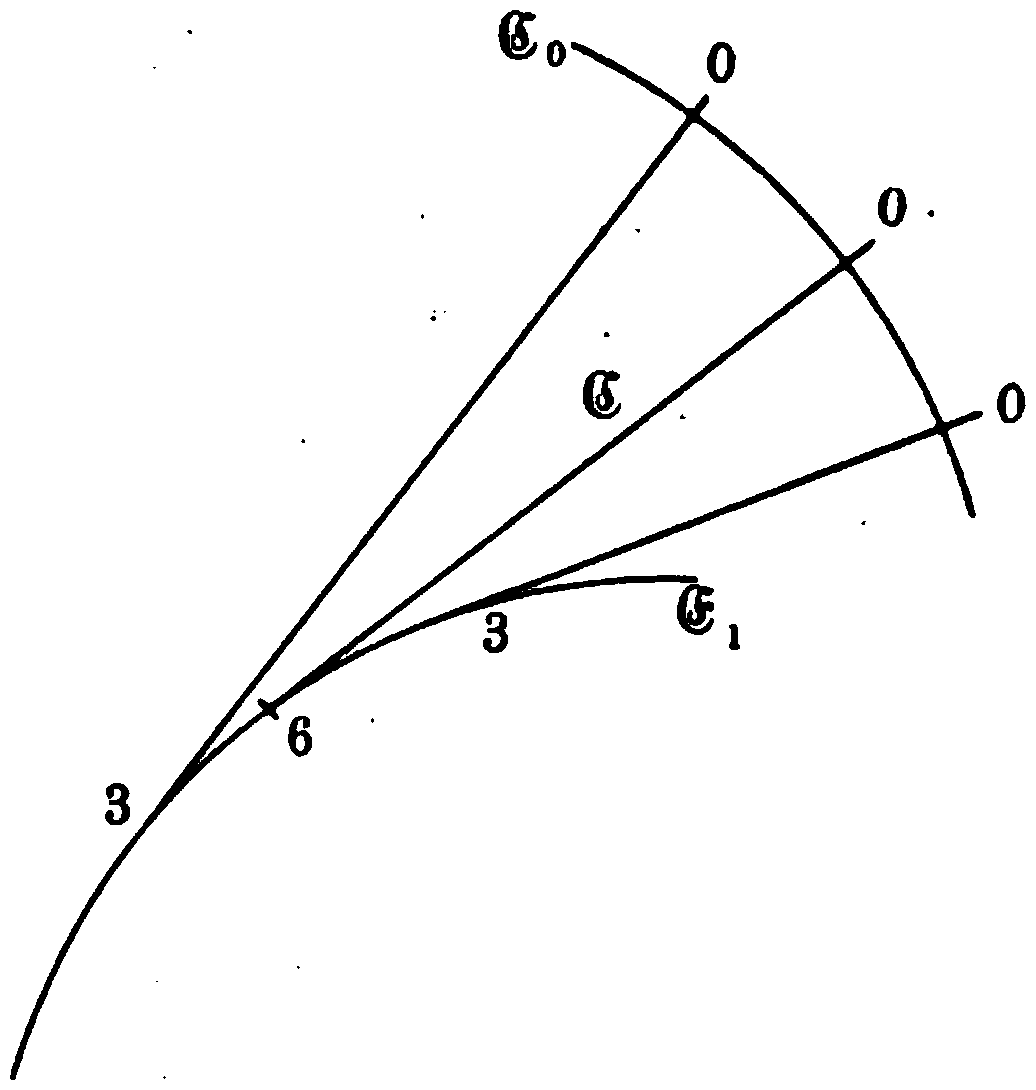
\includegraphics[width=\linewidth,height=38mm,keepaspectratio]{fig_assets/fig12_src_clean_x8.png}
\end{minipage}\hfill
\begin{minipage}[c]{0.49\linewidth}\centering
\end{minipage}
\end{center}
\[
Dx=\frac{dx}{da}\,da=\left(\xi_a+\xi_t\frac{dt}{da}\right)da
=\frac{\xi_t\Delta_a-\xi_a\Delta_t}{-\Delta_t}\,da,
\]
\[
Dy=\frac{dy}{da}\,da=\left(\eta_a+\eta_t\frac{dt}{da}\right)da
=\frac{\eta_t\Delta_a-\eta_a\Delta_t}{-\Delta_t}\,da;
\]
since now $\xi_t$ and $\eta_t$ do not vanish simultaneously, the equation (76) can be written in one of the forms
\[
\eta_a=\frac{\eta_t\xi_a}{\xi_t},
\quad
\xi_a=\frac{\xi_t\eta_a}{\eta_t}
\]
% src-pdfpage=0116
% src-break=0116
and from this one of the double equations
\begin{equation}\tag{78}
\begin{aligned}
Dy&=\frac{\eta_t}{\xi_t}\left(\xi_a+\xi_t\frac{dt}{da}\right)da=\frac{\eta_t}{\xi_t}Dx,\\
Dx&=\frac{\xi_t}{\eta_t}\left(\eta_a+\eta_t\frac{dt}{da}\right)da=\frac{\xi_t}{\eta_t}Dy
\end{aligned}
\end{equation}
can be inferred; thus the curve $\mathfrak{C}$ is touched at each of its points which are sufficiently little distant from 6 by that extremal of the field which belongs to the same value of $a$ as the point under consideration. The curve is therefore the envelope of the extremals of the field, and the existence of such an envelope under the assumptions introduced has been proved.

Along the curve $\mathfrak{C}$ one now approaches the point 6 belonging to $a=a_0$ if one increases $a$ by $da$ and assumes
\begin{equation}\tag{79}
(a-a_0)da<0.
\end{equation}
If further $\xi_t$ does not vanish at the point 6 and
\begin{equation}\tag{80}
\xi_t\frac{dx}{da}\bigg|^6(a-a_0)<0,
\quad
\left|\frac{dx}{da}\right|^6>0,
\end{equation}
then under the assumption (79)
\[
\xi_t\frac{dx}{da}\bigg|^6 da>0;
\]
with the sign of the quantity $a-a_0$ determined by the relation (80), the quantities $\xi_t$ and $Dx$ therefore have the same sign, and the motion along the curve $\mathfrak{C}$ directed toward the point 6 agrees with the direction of increasing $t$ along the tangent extremal. The half of the curve $\mathfrak{C}$ for which the inequality (80) holds we call $\mathfrak{C}_1$; along it one has, by (78), the two equations
\begin{equation}\tag{81}
Dx=\alpha\xi_tdt=\alpha dx,
\quad
Dy=\alpha\eta_tdt=\alpha dy,
\end{equation}
where $\alpha$ is positive. The existence of such an arc $\mathfrak{C}_1$ becomes doubtful only in the case
\[
\frac{dx}{da}\bigg|^6=0,
\quad
\left.\xi_t\Delta_a-\xi_a\Delta_t\right|^6=0,
\]
in which also the equation
\[
\Delta_t\frac{dy}{da}\bigg|^6=\eta_t\Delta_a-\eta_a\Delta_t
=\left.\eta_t\left(\Delta_a-\frac{\Delta_t\xi_a}{\xi_t}\right)\right|^6=0
\]
holds. Then possibly (Fig.~13) the curve $\mathfrak{C}$ has a cusp at the point 6; only if both branches go out from
% src-pdfpage=0117
% src-break=0117
the point 6 in the direction which corresponds to increasing values of $t$ on the curve $\mathfrak{C}$ is no arc $\mathfrak{C}_1$ present. We designate this as the exceptional case.

% unit: fig13 source=kneser_lvr_1900_archiveorg.pdf#p0117 authorial=true type=hq_sourcecrop
\begin{center}
{\small Fig.~13.}\par\vspace{1mm}
\begin{minipage}[c]{0.47\linewidth}\centering
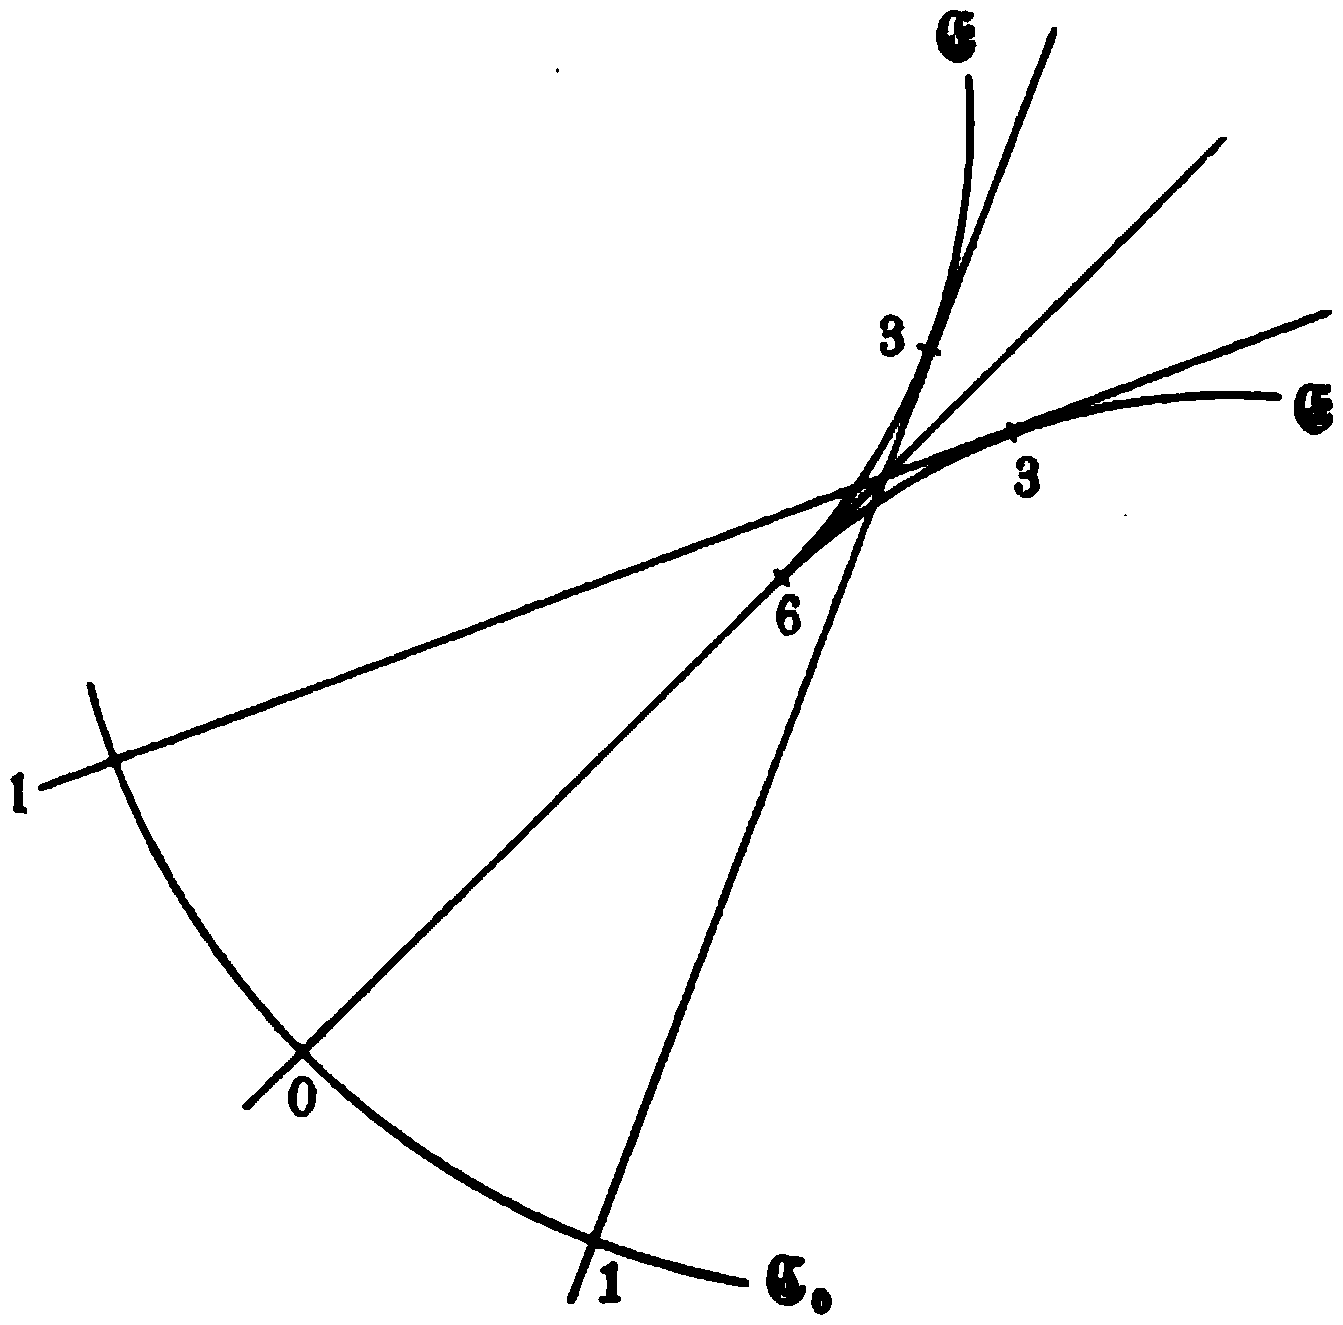
\includegraphics[width=\linewidth,height=38mm,keepaspectratio]{fig_assets/fig13_src_clean_x8.png}
\end{minipage}\hfill
\begin{minipage}[c]{0.49\linewidth}\centering
\end{minipage}
\end{center}

As before, let 0 be a point of the curve $\mathfrak{C}_0$ and 3 a point lying with it on the same extremal of the field, to which the arguments $a$ and $t$ refer. Then the quantity
\[
u=\overline{J}_{03}=\int_0^3F(\xi,\eta,\xi_t,\eta_t)dt
\]
is, not only as we know, in the field, but also in that region $\mathfrak{B}'$ a regular function of $a$ and $t$, in which the quantities $\xi,\eta,F(\xi,\eta,\xi_t,\eta_t)$ remain regular. The equations
\[
\frac{\partial u}{\partial a}=F_{x'}(\xi,\eta,\xi_t,\eta_t)\xi_a
+F_{y'}(\xi,\eta,\xi_t,\eta_t)\eta_a,
\]
\[
\frac{\partial u}{\partial t}=F(\xi,\eta,\xi_t,\eta_t),
\]
which were first derived for the field, therefore also hold in the region $\mathfrak{B}'$, since in this region their right and left sides remain regular functions of $a$ and $t$. In particular, let 3 be a point of the curve $\mathfrak{C}$; then, in proceeding along it, one has
\[
\begin{aligned}
du={}&F_{x'}(\xi,\ldots,\eta_t)(\xi_a da+\xi_tdt)
+F_{y'}(\xi,\ldots,\eta_t)(\eta_ada+\eta_tdt)\\
={}&F_{x'}(\xi,\ldots,\eta_t)Dx+F_{y'}(\xi,\ldots,\eta_t)Dy.
\end{aligned}
\]
On the other hand, along the curve $\mathfrak{C}$ form the integral
\[
J_{36}=\int_3^6F(x,y,Dx,Dy),
\]
so that the sign $D$ corresponds to the motion along the curve $\mathfrak{C}$ directed toward the point 6. Then
\[
dJ_{36}=-F(x,y,Dx,Dy)=-F(\xi,\eta,Dx,Dy).
\]
This quantity is opposite to the one obtained for $du$ if one can apply the homogeneity equations
% src-pdfpage=0118
% src-break=0118
\[
F_{x'}(\xi,\eta,\xi_t,\eta_t)=F_{x'}(\xi,\eta,Dx,Dy),
\]
\[
F_{y'}(\xi,\eta,\xi_t,\eta_t)=F_{y'}(\xi,\eta,Dx,Dy),
\]
that is, if the equations (81) hold and $\alpha$ is positive, so that the point 3 belongs to the arc $\mathfrak{C}_1$. In this case one has the equations
\[
\begin{aligned}
F_{x'}(\xi,\ldots,\eta_t)Dx+F_{y'}(\xi,\ldots,\eta_t)Dy
={}&F_{x'}(\xi,\eta,Dx,Dy)Dx\\
&+F_{y'}(\xi,\eta,Dx,Dy)Dy\\
={}&F(\xi,\eta,Dx,Dy),
\end{aligned}
\]
\[
du+dJ_{36}=d(\overline{J}_{03}+J_{36})=0.
\]
Now, if the distance of the points 3 and 6 becomes infinitely small, and with it the extremals 03 and $\mathfrak{C}$ coincide, evidently the equation
\[
\lim(\overline{J}_{03}+J_{36})=\overline{J}_{06}
\]
holds, and thus one obtains generally
\begin{equation}\tag{82}
\overline{J}_{03}+J_{36}=\overline{J}_{06}.
\end{equation}
If the curve $\mathfrak{C}$ contracts into the point 6, then evidently one obtains
\[
J_{36}=0.
\]
The values of $\overline{J}_{06}$ on the various extremals of the field are therefore equal.

Now the curve 036, which consists of the extremal arc 03 and the piece 36 belonging to the curve $\mathfrak{C}_1$, may be regarded as belonging to the closer neighborhood of the arc 06; for as soon as the distance 36 has become sufficiently small, the tangents of the arc 36 are arbitrarily little different from that of the point 6, and the tangents of the extremal 03, which passes continuously into that of the arc 06, are arbitrarily little different from the tangents of the latter. The arc 036 therefore belongs to those curves $\Omega$ with which the arc 06 would have to be compared if this arc were to make the integral $J$ even only a weak extremum in comparison with other lines joining the curve $\mathfrak{C}_0$ and the point 6. Then the difference
\[
J_{06}-J_{036}=J_{06}-(J_{03}+J_{36})
\]
would have to have a fixed sign without vanishing, whereas by (82) it has the value zero. The extremal arc 06 therefore surely supplies no extremum of the integral $J$, not even a weak one; rather the extremum ceases at the point 6 in the manner described more precisely by the equation (82). Thus, assuming the existence of the field, the following result is proved.

% src-pdfpage=0119
% src-break=0119
If the regular curve $\mathfrak{C}_0$ is cut transversally by the extremal $\mathfrak{C}$ at the point 0, and the latter is traversed by the point 5, then the arc 05 ceases to furnish a weak extremum of the integral $J$ among the lines going from the point 5 to the curve $\mathfrak{C}_0$ as soon as the point 5 moves into the focal point of the curve $\mathfrak{C}_0$. The same is true, if the curve $\mathfrak{C}_0$ contracts into a point 0, with respect to the extremum among the curves joining the fixed points 0 and 5, as soon as the point 5 passes into the point conjugate to 0. An exception occurs only when the always present envelope of the curves of the field possesses at the focal point a cusp of a special kind; in this case our consideration teaches that in an arbitrary neighborhood of the extremal piece bounded by two conjugate points there lie other such pieces which have the initial point in common with it, and are so constituted that they surely no longer furnish an extremum. In Fig.~13, for example, one evidently has
\[
\overline{J}_{13}=\overline{J}_{06}+J_{63}.
\]

% unit: sec26 source=kneser_lvr_1900_archiveorg.pdf#p0119 authorial=true
\begin{center}{\large \S~26.}\end{center}

\noindent\textbf{Example.} In the rectilinear elastic oscillation of a material point Hamilton's principle leads to the integral
\[
J=\int dx\,(p^2-y^2),
\]
whose extremals are determined by the simple equation
\[
\frac{dp}{dx}+y=0.
\]
The extremals
\[
y=a\sin x
\]
all pass through the fixed point $0\ (x=y=0)$, into which we think of the curve $\mathfrak{C}_0$ as contracted. If one puts $a=t$, then one obtains
\[
\Delta=\frac{\partial(x,a\sin x)}{\partial(x,a)}=\sin x;
\]
therefore for the point 6 conjugate to the point 0 one has $x=\pi$, and in its neighborhood $x$ and $a\sin x$ are evidently regular functions. The curve $\mathfrak{C}$ contracts into the point 6, since all extre-
% src-pdfpage=0120
% src-break=0120
mals of the considered family pass through it. The integrals $J$ obtained along them have equal value:
\[
J_{06}=\int_0^\pi a^2dx(\cos^2x-\sin^2x)
=\frac{a^2\sin2x}{2}\bigg|_0^\pi=0.
\]
The same case occurs for the great circles of the sphere as shortest lines; to every point the diametrically opposite point is conjugate. On the geodesic lines of a triaxial ellipsoid issuing from one umbilic point, the diametrically opposite umbilic point is conjugate to the initial point, and the two geodesic arcs joining them are of equal length.

The simplest example for the general equation (82) is supplied by the fundamental property of the evolute, by whose arc the difference of the radii of curvature of the evolvent corresponding to its end points is to be measured. One obtains this theorem by applying the equation (82) to Problem I and by considering the evolute as the curve $\mathfrak{C}_0$.

\noindent\textbf{Problem VI (\S~11).} A similarity transformation whose center lies on the $x$-axis and has abscissa $x_0$ is defined by the equations
\[
\bar y=\alpha y,
\quad
\bar x-x_0=\alpha(x-x_0),
\quad
\bar x=\alpha x-(\alpha-1)x_0.
\]
If therefore by the equations
\[
y=\frac{a(1+p^2)^2}{2p^3},
\quad
x=b+\frac{a}{2}\left(\frac{3}{4p^4}+\frac{1}{p^2}+\lg p\right)
\]
one has represented an extremal, then the point $(\bar x,\bar y)$ likewise describes an extremal. An arbitrary tangent to such an extremal has, when $X,Y$ are running coordinates, the equation
\[
Y-y=p(X-x),
\]
and hence cuts the $x$-axis in a point $T$ whose abscissa is
\[
X=x-\frac{y}{p}.
\]
Since then, from this,
\[
\frac{dX}{dp}=\frac{y}{p^2},
\]
and the values $p=0,p=+\infty$ give for $X$ the corresponding values $-\infty,+\infty$, the point $T$, if $a$ and therefore $y$ is positive, traverses the $x$-axis exactly once in the positive sense when
% src-pdfpage=0121
% src-break=0121
$p$ runs through all positive values increasing, and hence the point of contact of the tangent under consideration traverses (\S~11) the whole curve.

Now let (Fig.~14) a straight line $\mathfrak{C}_0$ be inclined at the acute angle $\psi$ to the $+x$-axis; then it is cut transversally by an extremal $\mathfrak{C}$ at the point 0 if at this point the equation
\[
\tg\psi=\frac{2p}{3+p^2}=\frac{p}{1+\frac12(1+p^2)}
\]
holds, which evidently gives
\begin{equation}\tag{83}
\tg\psi<p.
\end{equation}
To a given value of $\tg\psi$ there belong two real values of $p$, whose product is 3, as soon as the inequality
\[
\tg\psi<\frac1{\sqrt3},\quad \psi<30^\circ
\]
holds; one of those values, which we use for the construction of $\mathfrak{C}$, is therefore smaller than $\sqrt3$ and belongs to a point of that branch of the extremal whose pieces give a minimum of the resistance (\S~18). If furthermore 7 is the point of intersection of the tangent to the extremal at the point 0 with the $x$-axis, and 8 the point of intersection of this axis with the straight line $\mathfrak{C}_0$, then by (83) the point 7 lies to the right of 8, that is, toward the positive side. Therefore, if a point traverses the constructed extremal $\mathfrak{C}$ starting from 0 in the direction of increasing $x$, hence of decreasing $p$, then the point $T$ moves from the position 7 toward $-\infty$, and hence in the meantime reaches the position 8; let the point of contact of the tangent to the curve $\mathfrak{C}$ passing through 8 be 6.

% unit: fig14 source=kneser_lvr_1900_archiveorg.pdf#p0121 authorial=true type=hq_sourcecrop
\begin{center}
{\small Fig.~14.}\par\vspace{1mm}
\begin{minipage}[c]{0.47\linewidth}\centering
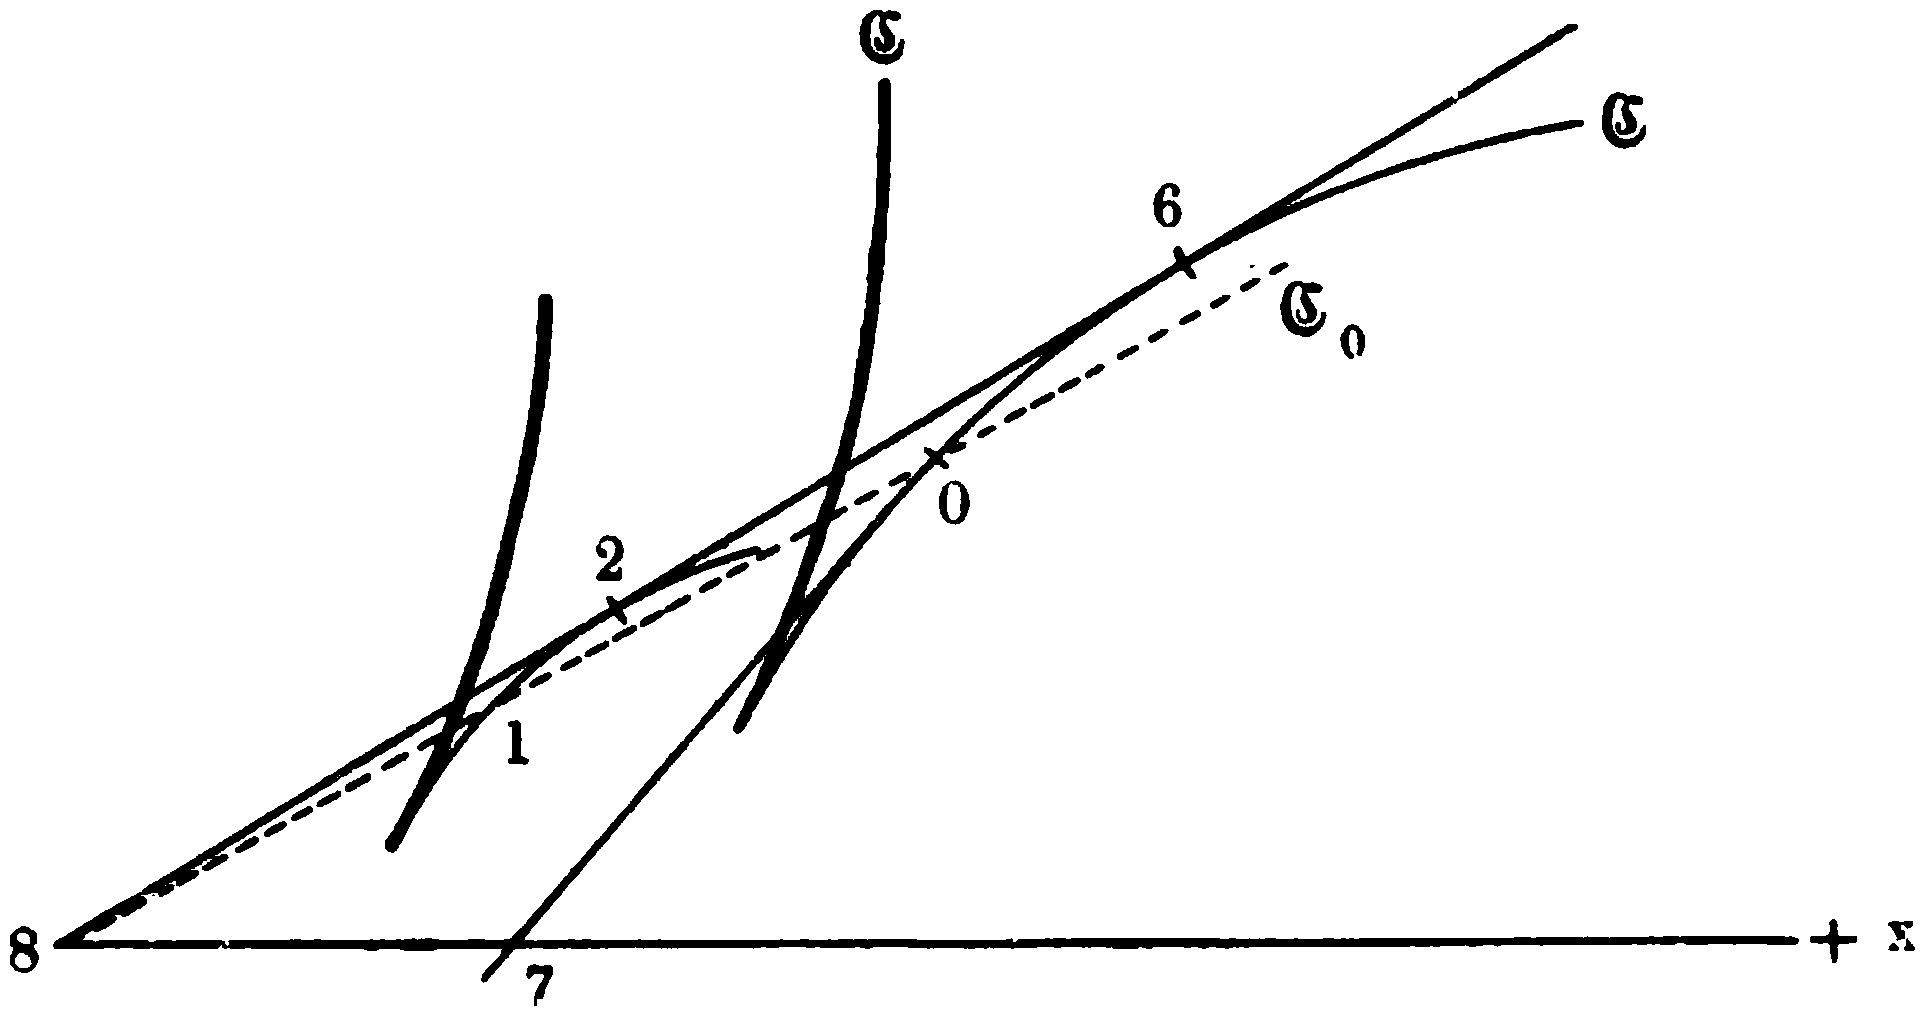
\includegraphics[width=\linewidth,height=36mm,keepaspectratio]{fig_assets/fig14_src_clean_x8.png}
\end{minipage}\hfill
\begin{minipage}[c]{0.49\linewidth}\centering
\end{minipage}
\end{center}

Make the point 8 now the center of a family of similarity transformations; these carry the curve $\mathfrak{C}$
% src-pdfpage=0122 portion=upper
% src-break=0122
into a family of extremals which cut the straight line $\mathfrak{C}_0$ transversally and touch the tangent 68. The latter therefore represents the envelope $\mathfrak{C}$ of the general theory, 6 is the focal point of the straight line $\mathfrak{C}_0$ on the curve $\mathfrak{C}$, and $\mathfrak{C}_1$ is the segment 68. If 2 is any point of this segment and the extremal of the constructed family touching it cuts the straight line $\mathfrak{C}_0$ at the point 1, then for the resistance integral the equation
\[
\overline{J}_{12}+J_{26}=\overline{J}_{06},
\]
holds, where $J_{26}$ is formed along the straight line 68. If therefore one lets the point 5 run along the curve $\mathfrak{C}$, then the arc 05 gives a weak minimum of the resistance, compared with the curves drawn from the point 5 to the straight line $\mathfrak{C}_0$, as long as the point 5 belongs to the arc 06; if it moves into the position 6, then the above equation shows in what manner, already for the arc 06, the minimum property is lost.

The method applied in Problem VI for the construction and delimitation of a field may be transferred to every problem in which the extremals of a family pass into one another through a known continuous group of transformations. Where the so-called orbit curves of the transformation touch the extremals of the family, there lie the boundaries of the field.


% machine-unit: sec27 source=kneser_lvr_1900_archiveorg.pdf#p0122 authorial=true
% src-pdfpage=0122 portion=lower
% src-break=0122
\begin{center}{\large \S~27.}\end{center}

That the extremals can be surrounded, at least piecewise, by fields is, in the individual problems, usually easy to see. But in order to be able to establish general theorems concerning these relations, we shall set up a function-theoretic consideration of general character, of which use will also be made later.

In the differential equations
\begin{equation}\tag{84}
\frac{dy}{dx}=f(x,y,z,\ldots),\quad
\frac{dz}{dx}=g(x,y,z,\ldots),\ldots,
\end{equation}
whose number is to be $n$, as is also the number of the unknowns $y,z,\ldots$, let the right hand sides be regular in the neighbourhood of the place
\begin{equation}\tag{85}
x=x_0,\quad y=Y_0,\quad z=Z_0,\ldots;
\end{equation}
% src-pdfpage=0123
% src-break=0123
then, as is well known, there exists an integral system whose members, for $x=x_0$, assume the arbitrarily prescribed values
\[
y=y_0,\quad z=z_0,\ldots
\]
as soon as the quantities
\[
|y_0-Y_0|,\quad |z_0-Z_0|,\ldots
\]
lie below a certain bound. For these integrals one obtains series by differentiating the equations (84) with respect to $x$, and by expressing on the right everything solely through functions of $x,y,z,\ldots$, after eliminating the differential quotients. If, in the expressions so obtained, which are likewise regular at the place (85), one substitutes for $x,y,z,\ldots$ the values $x_0,y_0,z_0,\ldots$, one obtains the coefficients of the Taylor developments of those determined solutions $y,z,\ldots$ according to powers of $x-x_0$. These coefficients are, as is shown in the proofs for the existence of the integrals, smaller in absolute value than the corresponding coefficients of a certain convergent power series of the argument $x-x_0$, which is independent of the special choice of the quantities $y_0,z_0,\ldots$. If, therefore, the latter are regarded as variable, then the series obtained for $y,z,\ldots$ converge uniformly in a certain domain; their values for a determined argument $x$ are therefore representable as power series in $y_0-Y_0,z_0-Z_0,\ldots$; evidently one can put
\[
\begin{aligned}
y&=y_0+(x-x_0)[x-x_0,y_0-Y_0,z_0-Z_0,\ldots]_0,\\
z&=z_0+(x-x_0)[x-x_0,y_0-Y_0,z_0-Z_0,\ldots]_0,\ldots,
\end{aligned}
\]
so that the functional determinant
\[
\frac{\partial(y,z,\ldots)}{\partial(y_0,z_0,\ldots)}
\]
obtains the value $1$ for $x=x_0$. The values of $y,z,\ldots$ for any determined argument $x$ are therefore mutually independent as functions of the quantities $y_0,z_0,\ldots$.

Now let the quantities $Y,Z,\ldots$ be defined as regular functions of $x$, satisfying the equations (84), in a real interval $\mathfrak J$ which is bounded below by the value $x_0$; for this value let
\[
Y=Y_0,\quad Z=Z_0,\ldots,
\]
and for $x=x_1$, on the other hand,
\[
Y=Y_1,\quad Z=Z_1,\ldots,
\]
and let every value-system $(x,Y,Z,\ldots)$ obtained in the interval $\mathfrak J$ belong to those in whose neighbourhood the functions $f,g,\ldots$
% src-pdfpage=0124
% src-break=0124
are regular. Then, in consequence of the preceding reasoning, there exist positive quantities $\delta,\varepsilon$ of such a character that an integral system regular in the interval
\begin{equation}\tag{86}
x_0\leq x\leq x_0+\varepsilon
\end{equation}
exists and, if $x_1$ denotes any place of this interval and if the inequalities
\[
|y_1-Y_1|<\delta,\quad |z_1-Z_1|<\delta,\ldots
\]
hold, assumes for $x=x_1$ the prescribed values $y_1,z_1,\ldots$. The values $y,z,\ldots$ at any determined place of the interval (86) are then regular, mutually independent functions of $y_1,z_1,\ldots$ in the neighbourhood of the value-system $(Y_1,Z_1,\ldots)$. Further, let $\gamma$ be the upper bound of all possible values $\varepsilon$; then the quantity
\[
\bar x=x_0+\gamma
\]
cannot lie in the interior of the interval $\mathfrak J$. For if this were the case, positive quantities $\bar\varepsilon,\bar\delta$ could be so determined that for the interval
\begin{equation}\tag{87}
-\bar\varepsilon<x-\bar x<\bar\varepsilon
\end{equation}
the quantity $\bar\delta$ would have the same significance as $\delta$ for the domain (86). But since the latter comes arbitrarily near to the point $\bar x$, there are in it places $x_1$ which belong at the same time to the domain (87); if, therefore, $\delta_1$ is the smaller of the quantities $\delta,\bar\delta$, and one assumes that
\[
|y_1-Y_1|<\delta_1,\quad |z_1-Z_1|<\delta_1,\ldots,
\]
then by every value-system $y_1,z_1,\ldots$ satisfying these inequalities an integral system is defined which is regular in the two domains (86), (87), hence in the whole domain
\[
x_0\leq x<\bar x+\bar\varepsilon
\]
and is so constituted that its values at a determined place are regular, mutually independent functions of the quantities $y_1,z_1,\ldots$. If one therefore put
\[
\varepsilon_1=\gamma+\bar\varepsilon,\quad \bar x+\bar\varepsilon=x_0+\varepsilon_1,
\]
then for the domain
\[
0\leq x-x_0<\varepsilon_1
\]
the quantity $\delta_1$ would have the same significance as $\delta$ for the domain (86); but this would contradict the notion of the upper bound, since $\varepsilon_1>\gamma$. The upper bound of all values $x_0+\varepsilon$ therefore lies outside the
% src-pdfpage=0125 portion=upper
% src-break=0125
interval $\mathfrak J$ or on its boundary. With the interval (86) every other interval can therefore be identified which, from $x_0$, reaches arbitrarily close to the boundary of the interval $\mathfrak J$.

It has hereby been shown that the integral manifold $(x,Y,Z,\ldots)$ can be surrounded by neighbouring ones in the following manner. There exist integrals
\[
y=\Phi(x,a,b,\ldots,k),\quad z=\Psi(x,a,b,\ldots,k),\ldots,
\]
which contain $n$ constants $a,b,\ldots,k$, and for a certain special value-system
\[
a=A,\quad b=B,\ldots,\quad k=K
\]
pass into the integrals $Y,Z,\ldots$; further, these are regular functions of their $n+1$ arguments as soon as $x$ belongs to the interior of the interval $\mathfrak J$ and the differences
\[
|a-A|,\quad |b-B|,\ldots,\quad |k-K|
\]
are sufficiently small. Under these hypotheses the functional determinant
\[
\frac{\partial(\Phi,\Psi,\ldots)}{\partial(a,b,\ldots)}
\]
is different from zero.

% machine-unit: sec28 source=kneser_lvr_1900_archiveorg.pdf#p0125 authorial=true
\begin{center}{\large \S~28.}\end{center}

In the integral
\[
J+\Delta J=\int F(x+\delta x,y+\delta y,x'+\delta x',y'+\delta y')\,dt
\]
let the integrand be developed according to Taylor's series; then the integral of twice the sum of all terms quadratic in the variations is
\[
\int dt\{F_{xx}\delta x^2+2F_{xy}\delta x\delta y+\cdots+F_{x'x'}\delta x'^2+\cdots\}.
\]
This expression arises from the variation
\[
\delta J=\int(F_x\delta x+F_y\delta y+F_{x'}\delta x'+F_{y'}\delta y')\,dt,
\]
by applying the operation $\delta$ according to the rules of differentiation and by regarding $t,\delta x,\delta x',\delta y,\delta y'$ as constant with respect to this operation. Accordingly one denotes that expression by $\delta^2J$ and calls it the second variation of $J$. If the variations $\delta x,\delta y$ contain a constant factor $\varepsilon$, then evidently
\begin{equation}\tag{88}
\Delta J=\delta J+\frac12\delta^2J+[\varepsilon]_3,
\end{equation}
% src-pdfpage=0126
% src-break=0126
and $\delta^2J$ contains the factor $\varepsilon^2$. Now one can put:
\[
\delta J=F_{x'}\delta x+F_{y'}\delta y+
\int dt(P\delta x+Q\delta y),
\]
therefore, since the sign $\delta$ is interchangeable with that of integration with respect to $t$, it follows that
\[
\delta^2J=\delta F_{x'}\delta x+\delta F_{y'}\delta y+
\int dt(\delta P\delta x+\delta Q\delta y),
\]
a formula which is very easily verified by calculation. In particular, in the case
\[
\left.\delta x\right|^0=\left.\delta x\right|^1=
\left.\delta y\right|^0=\left.\delta y\right|^1=0
\]
one obtains
\[
\delta^2J_{01}=\int_0^1dt(\delta P\delta x+
\delta Q\delta y).
\]

This formula is to be applied to a normal variation which is defined by the equations
\[
\delta x=\omega X,
\quad
\delta y=\omega Y,
\]
where $X,Y$ have the same meaning as in \S~24, and where $\omega$ vanishes at the places 0 and 1. Then, according to the identity (75) derived there,
\begin{equation}\tag{89}
\delta^2J_{01}=\int_0^1\omega(X\delta P+Y\delta Q)\,dt
=\int_0^1\omega\left(F_2\omega-\frac{d(F^1\omega')}{dt}\right)dt
\end{equation}
or, after an integration by parts,
\begin{equation}\tag{90}
\delta^2J_{01}=\int_0^1dt\,(F^1\omega'^2+F_2\omega^2).
\end{equation}

Now let 0 and 6 again be conjugate points; let the arc 02 extend beyond the latter. Then, according to \S~24, the equation
\begin{equation}\tag{91}
F_2\omega-\frac{d(F^1\omega')}{dt}=0
\end{equation}
has an integral vanishing at the points 0 and 6 and changing its sign at the point 6; let the arc 02 be so bounded that 0 and 6 are the only zeroes of the integral $\omega$ which belong to it. If $\varepsilon$ is then a sufficiently small constant and $F^1$ is different from zero along the whole arc 02, then the equation
\[
(F_2-\varepsilon)w-\frac{d(F^1w')}{dt}=0
\]
has, by \S~27, an integral which, like $\omega$, is regular on the segment 02, satisfies the equation
% src-pdfpage=0127
% src-break=0127
\[
\left.w\right|^0=\left.\omega\right|^0=0,
\]
and likewise possesses between 0 and 2 a single zero 7, which for $\varepsilon=0$ coincides with 6. Then, according to the general formulae (89), for the normal variation
\[
\delta x=Xw\alpha,
\quad
\delta y=Yw\alpha,
\]
in which $\alpha$ is constant, one has the formula
\[
\delta^2J_{07}=\alpha^2\int_0^7 w\left(F_2w-\frac{d(F^1w')}{dt}\right)dt
=\alpha^2\varepsilon\int_0^7w^2dt.
\]
If, therefore, one sets in the interval 72
\[
\delta x=\delta y=0,
\]
then, since for sufficiently small $\varepsilon$ the point 7 belongs to the interior of the interval 02, one has
\[
\delta^2J_{02}=\delta^2J_{07}=\alpha^2\varepsilon\int_0^7\omega^2dt,
\]
and since the varied curve is an extremal, by (88)
\[
\delta J_{02}=0,
\quad
\Delta J_{02}=\frac12\delta^2J_{07}+[\alpha]_3
=\frac{\alpha^2\varepsilon}{2}\int_0^7w^2dt+[\alpha]_3.
\]
This quantity evidently has, as soon as $\alpha$ is small enough, the sign in common with $\varepsilon$, and can therefore become both positive and negative, so that the arc 02 certainly does not yield an extremum of the integral $J$.

This consideration, which in its fundamental thoughts derives from Erdmann and Weierstrass, differs from those given in \S\S~24, 25 in that the latter in general already prove that the extremum is not present for an arc bounded by two conjugate points, but exclude an exceptional case; the development just carried out also extends to the exceptional case, but always requires that the arc considered extend beyond the point conjugate to its initial point.

If the arc 01 contains no pair of conjugate points, and $F^1$ does not vanish on it, formula (90) teaches that the sign of the second variation agrees with that of the quantity $F_1$ or $F^1$. For if $u$ is a function of $t$ regular from $t_0$ to $t_1$, one evidently has
\[
\int_0^1(u'\omega^2+2u\omega\omega')\,dt
=\int_0^1\frac{d}{dt}(u\omega^2)\,dt
=u\omega^2\bigg|_0^1=0,
\]
% src-pdfpage=0128
% src-break=0128
\begin{equation}\tag{92}
\delta^2J_{01}=\int_0^1dt\,[F^1\omega'^2+2u\omega\omega'+(F_2+u')\omega^2],
\end{equation}
and in this expression the integrand has the same sign as $F_1$, if one can determine $u$ according to the equation
\begin{equation}\tag{93}
(F_2+u')F^1-u^2=0;
\end{equation}
then one simply has
\begin{equation}\tag{94}
\delta^2J_{01}=\int_0^1F^1\left(\omega'+\frac{u\omega}{F^1}\right)^2dt.
\end{equation}
But the equation (93), like every equation of the form
\[
u'=Lu^2+Mu+N,
\]
can be reduced to a linear differential equation of the second order; by putting
\[
u=-\frac1L\frac{\omega'}{\omega},
\]
one obtains
\[
\omega''-\left(M+\frac{L'}L\right)\omega'+LN\omega=0;
\]
starting from equation (93), one arrives in this way precisely at equation (91), which is satisfied by the quantity $\Delta(t,a):\sqrt{\xi_t^2+\eta_t^2}$. Under the hypothesis introduced, this is different from zero along the arc 01, and thus gives a quantity $u$ regular in the interval of integration:
\[
u=-\frac{F_1\sqrt{\xi_t^2+\eta_t^2}}{\Delta(t,a)}\frac{d}{dt}\left(\frac{\Delta(t,a)}{\sqrt{\xi_t^2+\eta_t^2}}\right).
\]
If, therefore, a family of extremals is known, then, for an arc of the hypothesized nature and for a normal variation, formula (94) can be explicitly constructed.

A proof for the occurrence of the extremum with respect to all curves which arise from $\mathfrak C$ through a normal variation and belong to a narrower neighbourhood is obtained if one replaces the equation (93), understanding by $\varepsilon$ a sufficiently small constant, by the following:
\[
(F_2+u')F^1-u^2=\varepsilon^2.
\]
By \S~27, when $\varepsilon$ is sufficiently small, this has, as does the former equation, an integral regular from 0 to 1; if one introduces it into formula (92), then the quadratic form standing under the integral sign is definite, and the formula
% src-pdfpage=0129 portion=upper
% src-break=0129
\[
\Delta J_{01}=\frac12\delta^2J_{01}+\int_0^1[\omega,\omega']_3\,dt
\]
easily shows that the extremum actually occurs.

% machine-unit: sec29 source=kneser_lvr_1900_archiveorg.pdf#p0129 authorial=true
\begin{center}{\large \S~29.}\end{center}

If 02 is any curve-piece which is regular in the neighbourhood of each of its points (\S~1), then along it $x$ and $y$ can always be represented as regular one-valued functions of a parameter $t$, for example of the arc length measured from 0 toward 2. This is defined by the equations
\[
\frac{dt}{dx}=\sqrt{1+\left(\frac{dy}{dx}\right)^2},
\quad
\frac{dt}{dy}=\sqrt{1+\left(\frac{dx}{dy}\right)^2}
\]
in which each of the square roots has the same sign as the differential standing under it in the denominator when one advances in the direction 02. Namely, if at the place 1 the quantity $dy:dx$ is finite, hence $y$ is a regular function of $x$, then the same holds for $\frac{dt}{dx}$, and this quantity is different from zero:
\[
\frac{dt}{dx}=\left.\frac{dt}{dx}\right|^1+[x-x_1]_1,
\quad
t-t_1=\left.\frac{dt}{dx}\right|^1(x-x_1)+[x-x_1]_2;
\]
but the second equation gives
\[
x-x_1=[t-t_1]_1,
\]
so that $x$ and $y$ are regular functions of $t$ at the place 1. The same result is of course obtained by a similar development if $dx:dy$ is finite and consequently $x$ is representable as a regular function of $y$. The stipulation about the signs of the square roots has the effect that $dt$ is always positive when one advances in the direction 02, so that different values of $t$ correspond to different points of the arc.

Now if the arc 02 forms a part of an extremal and defines only value-systems $(x,y,x',y')$ in whose neighbourhood the integrand $F$ is regular, then the equations
\[
x'^2+y'^2=1,
\quad
F_1=F^1,
\quad
F_x-F_{x'}'=F_y-F_{y'}'=0
\]
hold, from which we derive the two equivalent systems:
\begin{equation}\tag{95}
\begin{aligned}
F_x-F_{x'x}x'-F_{x'y}y'-F_{x'x'}x''-F_{x'y'}y''&=0,\\
x'x''+y'y''&=0;
\end{aligned}
\end{equation}
% src-pdfpage=0130
% src-break=0130
\begin{equation}\tag{96}
\begin{aligned}
F_y-F_{y'x}x'-F_{y'y}y'-F_{y'x'}x''-F_{y'y'}y''&=0,\\
x'x''+y'y''&=0.
\end{aligned}
\end{equation}
From each of them $x'',y''$ can be calculated as functions of $x,y,x',y'$, and appear as fractions whose numerators are functions of $t$ regular along the arc 02, and whose denominators are the determinants
\[
\begin{vmatrix}
F_{x'x'}&F_{x'y'}\\
x'&y'
\end{vmatrix},
\quad
\begin{vmatrix}
F_{y'x'}&F_{y'y'}\\
x'&y'
\end{vmatrix}
\]
which, taking account of the identities derived in \S~16, can be brought into the following form:
\[
F_1y'(x'^2+y'^2)=F_1y'=\frac{\bar f_{qq}}{y'^2},
\quad
F_1x'(x'^2+y'^2)=F_1x'=\frac{f_{pp}}{x'^2}.
\]
If, therefore, we again introduce the restriction valid in \S~17, namely that for every line element of the arc 02 the quantity $F_1$ is different from zero, whereby certain singular solutions of the equations (95), (96) may possibly be excluded, then for $x''$ and $y''$, according as one uses one or the other of the systems (95), (96) as basis, one obtains expressions which are regular in the neighbourhood of every value-system $(x,y,x',y')$ defined by an element of the arc 02. If one writes for these expressions
\[
\frac{dx'}{dt}=M(x,y,x',y'),
\quad
\frac{dy'}{dt}=N(x,y,x',y')
\]
and adds the equations
\[
\frac{dx}{dt}=x',
\quad
\frac{dy}{dt}=y',
\]
whose right hand sides are always regular, then one obtains a system of the nature considered in \S~27, in which $x$ is replaced by $t$, and the interval $\mathfrak J$ extends from $t_0$ or 0 to $t_2$. There is therefore an integral system of the form
\begin{equation}\tag{97}
x=X(t,a,b,\alpha,\beta),
\quad
y=Y(t,a,b,\alpha,\beta),
\end{equation}
in which the functions $X,Y$ are regular as soon as $t$ belongs to the indicated interval, and the differences
\[
|a-x_0|,
\quad
|b-y_0|,
\quad
|\alpha-x'_0|,
\quad
|\beta-y'_0|
\]
are sufficiently small; here the identities
\begin{equation}\tag{98}
\begin{aligned}
X(0,a,b,\alpha,\beta)&=a,
&X_t(0,a,b,\alpha,\beta)&=\alpha,\\
Y(0,a,b,\alpha,\beta)&=b,
&Y_t(0,a,b,\alpha,\beta)&=\beta
\end{aligned}
\end{equation}
hold. If one therefore introduces the condition
% src-pdfpage=0131 portion=upper
% src-break=0131
\[
\alpha^2+\beta^2=1,
\]
then, by the second equation (95), one has in general
\[
X_t^2+Y_t^2=1,
\]
and the quantity $t$ also represents on all curves
\[
x=X,
\quad
y=Y
\]
the arc length measured from the point $(a,b)$ onward.

% machine-unit: sec30 source=kneser_lvr_1900_archiveorg.pdf#p0131 authorial=true
\begin{center}{\large \S~30.}\end{center}

Let us now posit the equation
\begin{equation}\tag{99}
\Gamma(a,b)=0
\end{equation}
which, if $a$ and $b$ are coordinates, represents a curve $\mathfrak C_0$ regular at the place $a=x_0,b=y_0$, along which $\Gamma_a$ and $\Gamma_b$ nowhere vanish simultaneously. Then the equations (97) define a family of extremals which issue from the points of the curve $\mathfrak C_0$ with the value $t=0$. They cut this curve transversally if the further assumption
\begin{equation}\tag{100}
\Lambda(a,b,\alpha,\beta)=\Gamma_bF_{x'}(a,b,\alpha,\beta)-\Gamma_aF_{y'}(a,b,\alpha,\beta)=0
\end{equation}
is introduced. Evidently one has
\[
\begin{aligned}
\Lambda_{\alpha}
&=\Gamma_bF_{x'x'}(a,b,\alpha,\beta)-\Gamma_aF_{y'x'}(a,b,\alpha,\beta)\\
&=\beta F_1(a,b,\alpha,\beta)(\alpha\Gamma_a+
\beta\Gamma_b),\\
\Lambda_{\beta}
&=-\alpha F_1(a,b,\alpha,\beta)(\alpha\Gamma_a+
\beta\Gamma_b);
\end{aligned}
\]
the functional determinant
\[
\frac{\partial(\Lambda,\alpha^2+\beta^2)}{\partial(\alpha,\beta)}
=2F_1(a,b,\alpha,\beta)(\alpha\Gamma_a+
\beta\Gamma_b)
\]
is therefore different from zero if this is true of the expression
\[
\alpha\Gamma_a+\beta\Gamma_b,
\]
and hence also if the quantity
\[
x'_0\Gamma_a(x_0,y_0)+y'_0\Gamma_b(x_0,y_0)
\]
does not vanish, that is, if the curve $\mathfrak C_0$ is not touched at the point 0 by the arc 02. This could only occur if the equations
\[
\begin{gathered}
x'_0\Gamma_a(x_0,y_0)+y'_0\Gamma_b(x_0,y_0)=0,\\
F_{y'}(x_0,y_0,x'_0,y'_0)\Gamma_a(x_0,y_0)
-F_{x'}(x_0,\ldots,y'_0)\Gamma_b(x_0,y_0)=0
\end{gathered}
\]
held together, from which the equation
\[
F(x_0,y_0,x'_0,y'_0)=0
\]
would follow. If we exclude this as in \S~15, then the equations
% src-pdfpage=0132
% src-break=0132
\begin{equation}\tag{101}
\alpha^2+\beta^2=1,
\quad
\Lambda(a,b,\alpha,\beta)=0
\end{equation}
give for $\alpha$ and $\beta$ regular expressions with the arguments $a,b$. Further, since equation (99) defines one of the quantities $a,b$ as a regular function of the other, for example $b$ as a function of $a$ if the inequality
\[
\Gamma_b(x_0,y_0)\gtrless0
\]
holds, all four constants occurring in $X$ and $Y$ therefore appear, on the basis of equations (99), (100), (101), expressed through $a$ alone, so that the equations of the extremal family assume the form
\[
x=X=\xi(t,a),
\quad
y=Y=\eta(t,a),
\]
and the functions $\xi$ and $\eta$ are regular at the place $(0,x_0)$. Here evidently
\[
\xi_t=X_t,
\quad
\xi_a=X_a+X_b\frac{db}{da}+X_{\alpha}\frac{d\alpha}{da}+X_{\beta}\frac{d\beta}{da},
\]
and these equations remain valid if one replaces $\xi$ by $\eta$ and $X$ by $Y$.

We now form the functional determinant
\[
2D=\frac{\partial(X,Y,\alpha^2+\beta^2,\Gamma,\Lambda)}{\partial(t,a,b,\alpha,\beta)}
=
\begin{vmatrix}
X_t&X_a&X_b&X_{\alpha}&X_{\beta}\\
Y_t&Y_a&Y_b&Y_{\alpha}&Y_{\beta}\\
0&0&0&2\alpha&2\beta\\
0&\Gamma_a&\Gamma_b&0&0\\
0&\Lambda_a&\Lambda_b&\Lambda_{\alpha}&\Lambda_{\beta}
\end{vmatrix}
\]
and take account of the fact that, by equations (98), one may put
\[
X=a+\alpha t+[t]_2,
\quad
Y=b+\beta t+[t]_2;
\]
then, for $t=0$, one obtains:
\[
\begin{gathered}
X_a=1,
\quad X_b=X_{\alpha}=X_{\beta}=0,
\quad X_t=\alpha,\\
Y_b=1,
\quad Y_a=Y_{\alpha}=Y_{\beta}=0,
\quad Y_t=\beta,
\end{gathered}
\]
and hence, on the basis of the above values $\Lambda_{\alpha},\Lambda_{\beta}$,
\[
D\big|_{t=0}=
\begin{vmatrix}
\alpha&1&0&0&0\\
\beta&0&1&0&0\\
0&0&0&\alpha&\beta\\
0&\Gamma_a&\Gamma_b&0&0\\
0&\Lambda_a&\Lambda_b&\beta&-\alpha
\end{vmatrix}
F_1(\alpha\Gamma_a+\beta\Gamma_b)
=-F_1(\alpha\Gamma_a+
\beta\Gamma_b)^2,
\]
% src-pdfpage=0133
% src-break=0133
a value which is evidently different from zero. If one now multiplies in $D$ the third, fourth, and fifth vertical rows by
\[
\frac{db}{da},\quad \frac{d\alpha}{da},\quad \frac{d\beta}{da}
\]
and adds them to the second, one obtains:
\[
\begin{aligned}
D
&=
\begin{vmatrix}
\xi_t&\xi_a\\
\eta_t&\eta_a
\end{vmatrix}
\begin{vmatrix}
0&\alpha&\beta\\
\Gamma_b&0&0\\
\Lambda_b&\Lambda_{\alpha}&\Lambda_{\beta}
\end{vmatrix}\\
&=
\begin{vmatrix}
\xi_t&\xi_a\\
\eta_t&\eta_a
\end{vmatrix}
\Gamma_bF_1(\alpha\Gamma_a+\beta\Gamma_b);
\end{aligned}
\]
hence also the quantity
\[
\Delta=\frac{\partial(\xi,\eta)}{\partial(t,a)}
\]
is different from zero in the neighbourhood of the place 0. The constructed extremals which cut the curve $\mathfrak C_0$ transversally therefore form, if one does not take them into consideration beyond a certain limit, a field of the arc 02, or of a finite part of it beginning at 0, exactly in the sense of \S~14.

The quantity $D$, when formed for the curves 02, contains only the first and second derivatives of $\Gamma$ for the value-system $a=x_0,b=y_0$; one easily concludes from this that any two curves $\mathfrak C_0$ which osculate at the point 0 have the same focal points on the extremal 02. If the curve $\mathfrak C_0$ contracts to a point 0, then $a$ and $b$ are no longer freely variable and can be omitted under the function signs $X,Y$. The determinant
\[
D_0(t)=
\begin{vmatrix}
X_t&X_{\alpha}&X_{\beta}\\
Y_t&Y_{\alpha}&Y_{\beta}\\
0&\alpha&\beta
\end{vmatrix}
=\frac{\partial(X,Y,\alpha^2+\beta^2)}{\partial(t,\alpha,\beta)}
\]
can, in consequence of equations (98), be written:
\[
D_0(t)=
\begin{vmatrix}
\alpha+[t]_1&t+[t]_2&[t]_2\\
\beta+[t]_1&[t]_2&t+[t]_2\\
0&\alpha&\beta
\end{vmatrix}
=\begin{vmatrix}
\alpha&t&0\\
\beta&0&t\\
0&\alpha&\beta
\end{vmatrix}+[t]_2=-t+[t]_2,
\]
it therefore vanishes at the point 0 itself, but not in its neighbourhood. If now, for example, $y'_0$ is different from zero, so that $\beta$ is regular as a function of $\alpha$ at the place $x'_0$, and if we set
% src-pdfpage=0134 portion=upper
% src-break=0134
\[
X(t,\alpha,\sqrt{1-\alpha^2})=\xi(t,\alpha),
\quad
Y(t,\alpha,\sqrt{1-\alpha^2})=\eta(t,\alpha),
\]
then $\xi$ and $\eta$ are regular at the place $(0,x'_0)$, and
\[
\alpha+\beta\frac{d\beta}{d\alpha}=0,
\]
\[
\xi_{\alpha}=X_{\alpha}+X_{\beta}\frac{d\beta}{d\alpha},
\quad
\eta_{\alpha}=Y_{\alpha}+Y_{\beta}\frac{d\beta}{d\alpha};
\]
from this it follows easily that
\[
D_0(t)=\frac{\partial(\xi,\eta)}{\partial(t,\alpha)}\beta=\beta\Delta.
\]
Hence $\Delta$ too is different from zero in the neighbourhood of the point 0, and if 1 is a point of the arc 02 lying sufficiently near to 0, then the arc 12 can at least in the neighbourhood of the point 1 be surrounded by a field whose extremals all pass through the point 0.

% machine-unit: sec31 source=kneser_lvr_1900_archiveorg.pdf#p0134 authorial=true
\begin{center}{\large \S~31.}\end{center}

If we restrict the four constants occurring in $X$ and $Y$ only by the relations
\[
\alpha^2+\beta^2=1,
\quad
\Gamma(a,b)=0,
\]
then we can express them through two constants, say $a$ and
\[
c=\frac{\beta}{\alpha},
\]
provided the quantities
\[
x'_0,
\quad
\Gamma_b(x_0,y_0)
\]
are different from zero. If we then obtain
\begin{equation}\tag{102}
x=\xi(t,a,c),
\quad
y=\eta(t,a,c),
\end{equation}
then $\xi$ and $\eta$ are regular at the place
\[
t=0,
\quad
a=x_0,
\quad
c=\frac{y'_0}{x'_0},
\]
and have the form
\[
\xi(t,a,c)=a+\frac{t}{\sqrt{1+c^2}}+[t]_2,
\]
\[
\eta(t,a,c)=b+\frac{ct}{\sqrt{1+c^2}}+[t]_2,
\]
where the square root has both times the same sign. Hence, for $t=0$, one obtains
% src-pdfpage=0135
% src-break=0135
\[
\frac{\partial(\xi,\eta)}{\partial(t,a)}=
\begin{vmatrix}
\dfrac{1}{\sqrt{1+c^2}}&1\\[1.2ex]
\dfrac{c}{\sqrt{1+c^2}}&\dfrac{db}{da}
\end{vmatrix}
=\frac{\dfrac{db}{da}-c}{\sqrt{1+c^2}};
\]
this value is, if the quantity
\[
\left|c-\frac{y'_0}{x'_0}\right|
\]
remains sufficiently small, different from zero, since by hypothesis the extremal $\mathfrak C$ and the curve $\Gamma=0$ do not touch each other. One can therefore represent the totality of all extremals which differ sufficiently little from a certain one, say $\mathfrak C$, in the neighbourhood of a determined point 0 belonging to the latter, in the form (102), where, if $\mathfrak C$ itself is obtained for $a=a_0,c=c_0$ and the parameter $t_{00}$ belongs to the point 0, the functions $\xi,\eta$ are regular at the place $(t_{00},a_0,c_0)$, and at least one of the quantities
\[
\theta_1(t,a,c)=\frac{\partial(\xi,\eta)}{\partial(t,a)},
\quad
\theta_2(t,a,c)=\frac{\partial(\xi,\eta)}{\partial(t,c)}
\]
is different from zero. However, the functions $\xi$ and $\eta$ need not necessarily have the special form indicated above, which proves the stated assertion only as a concrete example.

If one now fixes attention specifically on the extremals passing through the point 0, then for them
\[
x_0=\xi(t_0,a,c),
\quad
y_0=\eta(t_0,a,c);
\]
in consequence of the hypothesis valid for the quantities $\theta$, these equations can be solved for $t_0$ and $a$ or for $t_0$ and $c$; if one has, say,
\[
\theta_2(t_{00},a_0,c_0)\gtrless0,
\]
then one obtains for $t_0-t_{00}$ and $c-c_0$ expressions of the form $[a-a_0]_1$, and the values formed with these,
\[
\xi(t,a,c)=\xi(t,a),
\quad
\eta(t,a,c)=\eta(t,a),
\]
are regular at the place
\[
t=t_{00},
\quad
a=a_0.
\]
Further, since
\[
\xi_t=\xi_t,
\quad
\xi_a=\xi_a+\xi_c\frac{dc}{da},
\quad
\eta_t=\eta_t,
\quad
\eta_a=\eta_a+\eta_c\frac{dc}{da},
\]
\[
\left.(\xi_tdt_0+\xi_ada+\xi_cdc)\right|^0=0,
\quad
\left.(\eta_tdt_0+\eta_ada+\eta_cdc)\right|^0=0,
\]
% src-pdfpage=0136
% src-break=0136
and the latter equations give
\[
\frac{dc}{da}=-\frac{\theta_1(t_0,a,c)}{\theta_2(t_0,a,c)},
\]
one obtains
\[
\Delta=\frac{\partial(\xi,\eta)}{\partial(t,a)}
=\theta_1(t,a,c)+\theta_2(t,a,c)\frac{dc}{da}
=\frac{D(t_0,t)}{\theta_2(t_0,a,c)},
\]
where it is put that
\[
D(t_0,t)=
\begin{vmatrix}
\theta_1(t,a,c)&\theta_2(t,a,c)\\
\theta_1(t_0,a,c)&\theta_2(t_0,a,c)
\end{vmatrix}
=-D(t,t_0).
\]
This expression considered by Weierstrass is also the determinant of the coefficients of $dt,dt_0,da,dc$ in the linear forms $dx_0,dy_0,dx,dy$; namely, one easily verifies the identity
\[
-D(t_0,t)=
\begin{vmatrix}
\xi_t(t)&0&\xi_a(t)&\xi_c(t)\\
\eta_t(t)&0&\eta_a(t)&\eta_c(t)\\
0&\xi_t(t_0)&\xi_a(t_0)&\xi_c(t_0)\\
0&\eta_t(t_0)&\eta_a(t_0)&\eta_c(t_0)
\end{vmatrix}.
\]
The expression obtained for $\Delta$ shows that Jacobi's condition of the extremum is fulfilled on any extremal for the arc 12 if the points 0, 1, 2 follow one another in the direction of increasing $t$ and if the equation
\[
D(t_0,t)=0
\]
has in the interval from $t_0$ to $t_2$ no other root than $t=t_0$. This form of Jacobi's condition uses the point 0 lying outside the investigated arc 12, an inconvenience which is to be remedied in the following manner. If $t$ and $t_0$ lie in the neighbourhood of a fixed value $t_1$, then one can develop
\begin{equation}\tag{103}
\begin{aligned}
D(t,t_0)&=[t-t_1,t_0-t_1]_1\\
&=[(t-t_0)+(t_0-t_1),t_0-t_1]_1
=\sum_a^{1,\infty}f_a(t_0)(t-t_0)^a;
\end{aligned}
\end{equation}
the coefficients of this series appear at first as functions of $t_0$ and $t_1$, but, like $D(t,t_0)$, must be independent of the latter argument. Further, since $\theta_1$ and $\theta_2$ can be regarded as special cases of the quantity $\Delta$, which by \S~24 does not vanish simultaneously with its derivative with respect to $t$, the same holds for $D(t,t_0)$ if this expression does not vanish identically, and it follows that
% src-pdfpage=0137
% src-break=0137
\[
|f_1(t_0)|>0.
\]
If, therefore, one restricts the quantity $t_0$ to a certain interval
\begin{equation}\tag{104}
|t_0-t_1|<\varepsilon,
\end{equation}
then the quantity $|f_1(t_0)|$ lies above a positive bound $\gamma$. In consequence of the original development (103), there are furthermore such positive constants $g,\rho$ that, under the hypothesis
\begin{equation}\tag{105}
|t_0-t_1|<\rho,
\quad
|t-t_1|<\rho,
\end{equation}
the inequality
\[
\frac1{a!}\left|\frac{\partial^aD(t_0,t)}{\partial t^a}\right|<g\rho^{-a}
\]
holds; and since the left hand side passes for $t=t_0$ into $|f_a(t_0)|$, it follows, under the first inequality (105), that
\[
|f_a(t_0)|<g\rho^{-a},
\]
\[
\left|\sum_{a=2}^{\infty}f_a(t_0)(t-t_0)^{a-1}\right|
<\frac{g}{\rho}\sum_{a=2}^{\infty}\left|\left(\frac{t-t_0}{\rho}\right)^{a-1}\right|.
\]
There is therefore a positive constant $\delta$, depending only on $g,\rho,\gamma$, but not on $t_0$, of such a character that, under the assumption
\[
|t-t_0|<\delta
\]
and the hypotheses (104), (105), the inequality
\[
\left|f_1(t_0)+\sum_{a=2}^{\infty}f_a(t_0)(t-t_0)^{a-1}\right|>0
\]
holds; therefore the equation
\[
D(t_0,t)=0
\]
has between $t_0-\delta$ and $t_0+\delta$ no other root than $t=t_0$.

Now let $t_0$ be taken so near to $t_1$ that not only the relations (104), (105) are fulfilled, but also, if $\delta_0$ is a constant lying between 0 and $\delta$, the inequalities
\begin{equation}\tag{106}
t_0<t_1<t_0+\delta,
\quad
t_0+\delta>t_1+\delta_0
\end{equation}
hold. Further suppose that the equation
\begin{equation}\tag{107}
D(t_1,t)=0
\end{equation}
in the interval from $t_1$ to $t_2$ has only the root $t=t_1$, and thus none at all in the interval from $t_1+\delta_0$ to $t_2$. Then the latter remains true, as soon as $|t_1-t_0|$ is sufficiently small, for the equation
\[
D(t_0,t)=0,
\]
% src-pdfpage=0138
% src-break=0138
which between $t_0-\delta$ and $t_0+\delta$, and consequently also by (106) between $t_0-\delta$ and $t_1+\delta_0$, possesses only the one root $t_0$; this is therefore also the only root of the last equation for the whole interval from $t_0$ to $t_2$. It has thereby been shown that, under the hypothesis introduced for equation (107), Jacobi's condition is fulfilled in the form given above, that is, that the extremals passing through a suitably chosen point 0 form a field of the arc 12. Jacobi's condition can therefore also, when the question is the extremum for the arc 12 with fixed end points, be replaced by the requirement that equation (107) have on the segment from $t_1$ to $t_2$ no other root than $t=t_1$.

If one can in particular set $x=t$, then one obtains
\[
y=\eta(x,a,c),
\quad
\theta_1=\frac{\partial y}{\partial a},
\quad
\theta_2=\frac{\partial y}{\partial c},
\]
\[
D(t_0,t)=\Delta(x_0,x)=
\begin{vmatrix}
\dfrac{\partial y}{\partial a}&\dfrac{\partial y}{\partial c}\\[1.2ex]
\left.\dfrac{\partial y}{\partial a}\right|^0&
\left.\dfrac{\partial y}{\partial c}\right|^0
\end{vmatrix};
\]
if one sets this expression equal to zero, one has the criterion of conjugate points in the form given by Hesse.



% src-pdfpage=0139
% src-break=0139
\begin{center}
{\large Fourth Section.}\par
\vspace{4mm}
{\Large\bfseries The simplest relative extremum.}\par
\vspace{2mm}\rule{26mm}{0.4pt}\par
\end{center}

\begin{center}{\large \S~32.}\end{center}

The isoperimetric problem in the wider sense of the word requires that an integral
\[
J=\int f(x,y,p)\,dx=\int F(x,y,x',y')\,dt
\]
be made an extremum when another integral of the same form
\[
K=\int g(x,y,p)\,dx=\int G(x,y,x',y')\,dt
\]
has a prescribed value; that is, among all curves which give the prescribed value to the integral $K$, one is to find that curve along which $J$ assumes an extreme value. Such an extremum is called a \textbf{relative} extremum; those considered up to now are, in contrast, \textbf{absolute} extrema. The isoperimetric problem in the narrower sense is obtained when $J$ is the area integral and $K$ is the arc length.

In order first to derive necessary conditions of this extremum, let $\mathfrak{B}$ be a piece of curve having the properties required in \S\S~2 and 4 for the arc denoted in the same way; let the functions $F$ and $G$ be regular for the systems of arguments defined by the elements of this arc. Along it let the points 0, 1, 2, 3 follow one another in the direction of increasing values of $t$; then we vary the two arcs 01 and 23 according to the method used in \S~8.

Let $\varepsilon,\eta,\bar\varepsilon,\bar\eta$ denote constants, and put
\[
T=(t-t_0)^3(t_1-t)^3,
\quad
U=(t-t_2)^3(t_3-t)^3,
\]
then for the arc 01 let
% src-pdfpage=0140
% src-break=0140
\[
\delta x=\varepsilon T,
\quad
\delta y=\eta T,
\]
and further for the arc 23
\[
\delta x=\bar\varepsilon U,
\quad
\delta y=\bar\eta U,
\]
while outside the segments 01 and 23 everywhere
\[
\delta x=\delta y=0.
\]
Since the first and second derivatives of the quantities $\delta x,\delta y$ vanish at the places 0, 1, 2, 3, the point $(x+\delta x,y+\delta y)$ describes a curve having the continuity properties presupposed for $\mathfrak{B}$. Clearly, in the notation of the first two sections, the equations
\begin{equation}\tag{1}
\Delta J=\Delta J_{01}+\Delta J_{23},
\quad
\Delta K=\Delta K_{01}+\Delta K_{23}
\end{equation}
hold; therefore, in order that along the varied curve the integral $K$ may have the same value as along the original one, the equation
\[
\Delta K=\Delta K_{01}+\Delta K_{23}=0
\]
has to be satisfied.

Put further
\[
P=F_x-F'_{x'},\quad Q=F_y-F'_{y'},\quad
R=G_x-G'_{x'},\quad S=G_y-G'_{y'},
\]
then, by \S~4, when the variations vanish at the limits of integration,
\[
\Delta J=\delta J+\int dt\,[\delta x,\delta y,\delta x',\delta y']_2,
\]
\[
\delta J=\int dt\,(P\delta x+Q\delta y),
\]
and analogous formulae hold for the integral $K$; hence, for the indicated special variation, on the basis of formulae (1), one obtains
\[
\begin{aligned}
\Delta J={}&\varepsilon\int_0^1PT\,dt+
\eta\int_0^1QT\,dt+
\bar\varepsilon\int_2^3PU\,dt+
\bar\eta\int_2^3QU\,dt\\
&+[\varepsilon,\eta,\bar\varepsilon,\bar\eta]_2,
\end{aligned}
\]
\[
\begin{aligned}
\Delta K={}&\varepsilon\int_0^1RT\,dt+
\eta\int_0^1ST\,dt+
\bar\varepsilon\int_2^3RU\,dt+
\bar\eta\int_2^3SU\,dt\\
&+[\varepsilon,\eta,\bar\varepsilon,\bar\eta]_2.
\end{aligned}
\]
If now the curve $\mathfrak{B}$ is to furnish a relative extremum of the integral $J$ in the defined sense, then $\Delta J$ must have a fixed sign for all varied curves for which $\Delta K$ vanishes. Since the constants $\varepsilon,\eta,\bar\varepsilon,\bar\eta$ are freely available, it follows from \S~7 that the second-order determinants which are formed from any two vertical columns of the scheme
% src-pdfpage=0141
% src-break=0141
\[
\begin{array}{cccc}
\displaystyle \int_0^1RT\,dt,&\displaystyle \int_0^1ST\,dt,&\displaystyle \int_2^3RU\,dt,&\displaystyle \int_2^3SU\,dt,\\[2.2ex]
\displaystyle \int_0^1PT\,dt,&\displaystyle \int_0^1QT\,dt,&\displaystyle \int_2^3PU\,dt,&\displaystyle \int_2^3QU\,dt,
\end{array}
\]
must vanish. Since the quantity $T$ is positive on the segment 01, and likewise $U$ on the segment 23, one can bring this scheme into the following form:
\[
\begin{array}{cccc}
\displaystyle R_m\int_0^1T\,dt,&\displaystyle S_m\int_0^1T\,dt,&\displaystyle R_\mu\int_2^3U\,dt,&\displaystyle S_\mu\int_2^3U\,dt,\\[2.2ex]
\displaystyle P_m\int_0^1T\,dt,&\displaystyle Q_m\int_0^1T\,dt,&\displaystyle P_\mu\int_2^3U\,dt,&\displaystyle Q_\mu\int_2^3U\,dt,
\end{array}
\]
where the suffix $m$ means that for $t$ a value of the interval from $t_0$ to $t_1$ is to be taken, and $\mu$ has the same meaning for the interval from $t_2$ to $t_3$. All the integrals occurring here are positive; thus all second-order determinants formed from vertical columns of the system
\begin{equation}\tag{2}
\begin{array}{cccc}
R_m,&S_m,&R_\mu,&S_\mu,\\
P_m,&Q_m,&P_\mu,&Q_\mu
\end{array}
\end{equation}
also vanish.

We now observe that, under the presupposed properties of the arc $\mathfrak{B}$, $P,Q,R,S$ are continuous functions of $t$; hence, if the segments 01 and 23 are indefinitely diminished while keeping the points 0 and 2 fixed, then the quantities bearing the suffixes $m$ and $\mu$ approach definite limiting values:
\[
\lim P_m=P_0,
\quad
\lim Q_m=Q_0,
\quad
\lim P_\mu=P_2,
\quad
\lim Q_\mu=Q_2,
\]
\[
\lim R_m=R_0,
\quad
\lim S_m=S_0,
\quad
\lim R_\mu=R_2,
\quad
\lim S_\mu=S_2,
\]
and for the second-order determinants formed from these quantities the same holds as for the quantities (2). In particular the equations
\[
P_0S_2-R_0Q_2=0,
\quad
Q_0S_2-S_0Q_2=0
\]
hold. We now introduce the supposition that the curve $\mathfrak{B}$ is not an extremal of either of the two integrals $J$ and $K$, so that neither the quantities $R$ and $S$ nor the quantities $P$ and $Q$ vanish everywhere along it. Then one can choose the point 2 so that one of the quantities $P_2,Q_2$, say $Q_2$, is different from zero, and the last equations give
% src-pdfpage=0142
% src-break=0142
\[
P_0\frac{S_2}{Q_2}-R_0=Q_0\frac{S_2}{Q_2}-S_0=0.
\]
If $S_2=0$, then from these equations, for arbitrary position of the point 0, it would follow that
\[
R_0=S_0=0,
\]
and the curve $\mathfrak{B}$ would therefore, contrary to the supposition, be an extremal of the integral $K$. Hence there is a finite quantity, different from zero and independent of the position of the point 0,
\[
\lambda=-\frac{Q_2}{S_2},
\]
with the property that the equations
\[
P_0+\lambda R_0=Q_0+\lambda S_0=0
\]
hold. The same conclusion results, if $P_2$ does not vanish, from the equations
\[
P_0R_2-R_0P_2=0,
\quad
Q_0R_2-S_0P_2=0.
\]
The curve $\mathfrak{B}$ therefore satisfies the differential equations
\[
F_x-F'_{x'}+\lambda(G_x-G'_{x'})=0,
\quad
F_y-F'_{y'}+\lambda(G_y-G'_{y'})=0,
\]
or, with the notation
\[
H=F+\lambda G,
\]
the equations
\[
H_x-H'_{x'}=0,
\quad
H_y-H'_{y'}=0,
\]
in which $\lambda$ denotes a finite constant different from zero. Every curve which, for arbitrary non-vanishing value of $\lambda$, satisfies these equations, we call an extremal for the proposed problem of the relative extremum; since one can divide the equations by $\lambda$, it is evident that the totality of extremals remains the same when the integrals $J$ and $K$ interchange their roles.

The result of the investigation can now be stated as follows: the curve which furnishes the sought relative extremum, under the presupposed continuity properties, can be nothing other than a piece of an extremal, unless it is perhaps an extremal for one of the integrals $J,K$ in the sense of the absolute extremum. We leave the latter exceptional case aside in the general theory.

% src-pdfpage=0143
% src-break=0143
\begin{center}{\large \S~33.}\end{center}

Let the integral $J$ be made an extremum in particular by a curve 01 whose endpoints are not given, but are restricted only in so far as between the coordinates $x_0,y_0,x_1,y_1$ some relations
\[
g_b(x_0,y_0,x_1,y_1)=0
\]
are prescribed, their number being no greater than four. A curve 01 solving this problem and having the properties of the arc $\mathfrak{B}$, which we assume to exist, must first of all, apart from the exceptional case indicated at the end of \S~32, be a piece of an extremal; for otherwise, by \S~32, one could vary it without moving its endpoints in such a way that $J$, while $K$ kept an unchanged value, would both increase and decrease. If then the endpoints too are to be varied, the equations
\begin{equation}\tag{3}
g_b(x_0+\delta x_0,\ldots,y_1+\delta y_1)=0
\end{equation}
must hold. In particular, along an arc 02 of the curve 01 we put
\[
\delta x=\delta x_0\left(\frac{t-t_2}{t_0-t_2}\right)^3,
\quad
\delta y=\delta y_0\left(\frac{t-t_2}{t_0-t_2}\right)^3
+\varepsilon(t_2-t)^3(t-t_0)^3,
\]
and along an arc 31 separated from it
\[
\delta x=\delta x_1\left(\frac{t-t_3}{t_1-t_3}\right)^3,
\quad
\delta y=\delta y_1\left(\frac{t-t_3}{t_1-t_3}\right)^3,
\]
while in the middle piece 23
\[
\delta x=\delta y=0.
\]
Then the variations along the whole curve 01, together with their first two derivatives, are continuous functions of $t$.

In general one has
\[
\Delta K_{01}=G_{x'}\delta x+G_{y'}\delta y\bigg|_0^1+
\int_0^1dt\{R\delta x+S\delta y\}
+[\delta x,\delta y,\delta x',\delta y']_2,
\]
hence for the indicated special variation
\[
\Delta K_{01}=[\delta x_0,\delta y_0,\delta x_1,\delta y_1]_1+
\varepsilon\int_0^2S(t_2-t)^3(t-t_0)^3\,dt
+[\varepsilon,\delta x_0,\delta y_0,\delta x_1,\delta y_1]_2.
\]
% src-pdfpage=0144
% src-break=0144
Here the factor of $\varepsilon$ is different from zero, since 01 is a regular curve on which the quantity $S$ has only separated zeros if it does not vanish everywhere; in the latter case, since the curve considered is not supposed to be an extremal of the integral $K$, the quantity $R$ cannot vanish everywhere along the curve 01, and one need only interchange $x$ and $y$ throughout the whole argument. Hence, if $S$ is at least at some places different from zero, one can choose the interval 02 so that $S$ remains different from zero in its interior. Then from the equation
\begin{equation}\tag{4}
\Delta K_{01}=0
\end{equation}
one can compute
\[
\varepsilon=[\delta x_0,\delta y_0,\delta x_1,\delta y_1]_1.
\]
On the other hand, under the supposition (4), one has
\[
\Delta J_{01}=\Delta(J_{01}+\lambda K_{01});
\]
by analogy with the formula for $\Delta K_{01}$, taking account of the equations of the extremals, one obtains from this
\[
\Delta J_{01}=H_{x'}\delta x+H_{y'}\delta y\bigg|_0^1+
\int_0^1dt\,[\delta x,\delta y,\delta x',\delta y']_2.
\]
For the defined special variation, substituting the above expression for $\varepsilon$, one therefore has
\[
\Delta J_{01}=H_{x'}\delta x+H_{y'}\delta y\bigg|_0^1+
[\delta x_0,\delta y_0,\delta x_1,\delta y_1]_2.
\]
If the required extremum is to be furnished by the curve 01, this quantity must have a fixed sign for all values $\delta x_0,\ldots,\delta y_1$ satisfying equations (3); this requires, by \S~7, that the equation
\[
H_{x'}\delta x+H_{y'}\delta y\bigg|_0^1=0
\]
be a consequence of the linear relations
\[
\frac{\partial g_b}{\partial x_0}\delta x_0+
\frac{\partial g_b}{\partial y_0}\delta y_0+
\frac{\partial g_b}{\partial x_1}\delta x_1+
\frac{\partial g_b}{\partial y_1}\delta y_1=0.
\]
If, in particular, $x_0,y_0$ are given and the point 1 is to lie on the curve
\[
h(x,y)=0,
\]
so that always
\[
\delta x_0=\delta y_0=0,
\]
then the equation
% src-pdfpage=0145
% src-break=0145
\[
H_{x'}\delta x+H_{y'}\delta y\bigg|^1=0
\]
must hold under the supposition
\[
h_x\delta x+h_y\delta y\bigg|^1=0.
\]
We then say that the extremal 01 cuts the curve $h=0$ \textbf{transversally}. That this occurs is a necessary condition for the extremal 01, among all lines drawn from the point 0 to the curve $h=0$ which yield the prescribed value $K_{01}$, to furnish an extremum of the integral $J$.

\begin{center}{\large \S~34.}\end{center}

\noindent\textbf{Examples. Problem IX.} To find the curve of given length which makes the area integral a maximum.

One has (\S~4), evidently with the positive square root,
\[
J=\int y\,dx=\int yx'\,dt,
\quad
K=\int dt\sqrt{x'^2+y'^2},
\]
\[
H=yx'+\lambda\sqrt{x'^2+y'^2},
\quad
H_x=0,
\]
therefore as equation of the extremals there first results
\begin{equation}\tag{5}
H_{x'}=y+\frac{\lambda x'}{\sqrt{x'^2+y'^2}}=a,
\quad
\frac{dx}{dy}=\frac{a-y}{\lambda\sqrt{1-\left(\dfrac{a-y}{\lambda}\right)^2}},
\end{equation}
and from this by integration
\[
\frac{x-b}{\lambda}=\sqrt{1-\left(\frac{a-y}{\lambda}\right)^2},
\quad
(y-a)^2+(x-b)^2=\lambda^2.
\]
The totality of all extremals is therefore identical with that of all circles of the plane, and the square of the isoperimetric constant is equal to that of the radius. If the endpoints 0, 1 are prescribed, then the integral $J$ is equal to the area between the curve 01 and the straight segment 01, increased by the constant area of the trapezoid swept out by the ordinates of the straight segment; hence, if the former area is to become a maximum, the required curve with the properties of the arc $\mathfrak{C}$ can be nothing other than a circular arc. The transversal position is defined by the equation
\[
H_{x'}Dx+H_{y'}Dy=
\left(y+\frac{\lambda x'}{\sqrt{x'^2+y'^2}}\right)Dx+
\frac{\lambda y'}{\sqrt{x'^2+y'^2}}Dy=0;
\]
on the $x$-axis ($y=0$) it passes into the more special form
% src-pdfpage=0146
% src-break=0146
\[
x'Dx+y'Dy=0.
\]
Thus if the required curve is to begin at the given point 0 and end at a non-prescribed point of the $x$-axis, then the area bounded by this axis, the ordinate of the point 0, and the required curve, for a given length of the latter, is in no other case a maximum than when the curve is a circular arc whose center lies on the $x$-axis. (Compare Problem III.)

If the required curve is closed, then the integral $J$, by \S~4, represents the area enclosed by it when one integrates exactly once around the curve; one then has the conditions
\[
x_0-x_1=y_0-y_1=0,
\quad
\delta x_0-\delta x_1=\delta y_0-\delta y_1=0,
\]
in consequence of which the condition
\[
H_{x'}\delta x+H_{y'}\delta y\bigg|_0^1=0
\]
is fulfilled by itself if the curve throughout its whole course has the properties of the arc $\mathfrak{B}$. Under this supposition it can therefore, for a given length, give an extreme content only if it is a circle.

If the content is to be not the area swept out by the ordinate, but the area enclosed by the required curve and by a given curve $\mathfrak{H}$
\[
y=h(x),
\]
then one has to put
\[
J=\int [y-h(x)]x'\,dt;
\]
then
\[
H=[y-h(x)]x'+\lambda\sqrt{x'^2+y'^2},
\]
and the quantities $H_y,H_{y'}$ and $H_x-H'_{x'}$ are therefore the same as in the preceding case, so that the extremals are still circles. The condition of transversal intersection is
\[
\left[y-h(x)+\frac{\lambda x'}{\sqrt{x'^2+y'^2}}\right]Dx+
\frac{\lambda y'}{\sqrt{x'^2+y'^2}}Dy=0;
\]
the curve $\mathfrak{H}$ therefore stands perpendicular to the extremals which cut it transversally. Geometrically this problem becomes most interesting when the endpoint 1, or also both endpoints 0 and 1, are non-prescribed points of the curve $\mathfrak{H}$; then
% src-pdfpage=0147
% src-break=0147
the solution, if such a solution exists, is a circle normal to the curve $\mathfrak{H}$ at one or two points.

The sign of the quantity $\lambda$ is determined by the first equation (5). Namely, if the direction of increasing $t$ is situated with respect to the outward-going radius of the circle in the same way as the $+y$-axis is situated with respect to the $+x$-axis, then, since $|\lambda|$ is always the radius of the circle, one has
\[
\frac{x'}{\sqrt{x'^2+y'^2}}=-\frac{y-a}{|\lambda|},
\]
hence $\lambda=|\lambda|$; the opposite results when the direction of increasing $t$ is situated with respect to the radius as the $+x$-axis is situated with respect to the $+y$-axis.

\medskip
\noindent\textbf{Problem X.} On a given surface, to draw a shortest possible line which, with a given curve or also, if it is closed, by itself alone, encloses a piece of given area (curves of shortest perimeter).

On the surface let $x$ and $y$ be isometric curvilinear coordinates, that is, let the position of a point be uniquely determined by these quantities in a certain region containing the point $x=y=0$; let the line element have the form
\[
ds=\sqrt{M(dx^2+dy^2)}.
\]
By the ordinate of a point $(x,y)$ we mean the piece of a line $x=\mathrm{const}$ drawn from it to the line $y=0$. Then $Mdx\,dy$ is the size of a quadrilateral surface element whose sides are elements of the lines $x=\mathrm{const}.$ and $y=\mathrm{const}.$ If therefore
\[
y=h(x)
\]
is the equation of any curve, then the area bounded by two adjacent ordinates of it is
\[
dx\cdot\int_0^ydy\,M=dx\,[N(x,y)-N(x,0)],
\]
where $N$ is a function of $x$ and $y$ satisfying the equation
\[
\frac{\partial N}{\partial y}=M.
\]
The total area which is covered by the ordinates of the curve $y=h(x)$, if one fixes attention on the arc 01, is accordingly
% src-pdfpage=0148
% src-break=0148
\[
\int_0^1dx\{N[x,h(x)]-N[x,0]\}.
\]
If then $(x,y)$ denotes a point of another curve 01, the area lying between the two is
\[
K=\int_0^1dx\{N[x,y]-N[x,h(x)]\};
\]
the integral to be made a minimum is
\[
J=\int_0^1dx\sqrt{M(1+p^2)};
\]
thus one has
\[
H=\sqrt{M(x'^2+y'^2)}+\lambda\{N[x,y]-N[x,h(x)]\}x',
\]
and the one equation of the extremals is
\[
H_y-H'_{y'}=\frac{M_y\sqrt{x'^2+y'^2}}{2\sqrt{M}}+
\lambda Mx'-\frac{d}{dt}\left(\frac{y'\sqrt{M}}{\sqrt{x'^2+y'^2}}\right)=0,
\]
or, if one defines the angle $\theta$ by the equations
\[
\cos\theta=\frac{x'}{\sqrt{x'^2+y'^2}},
\quad
\sin\theta=\frac{y'}{\sqrt{x'^2+y'^2}},
\]
\[
\lambda Mdx=d(\sqrt{M}\sin\theta)-\frac{ds}{\sqrt{M}}\frac{\partial\sqrt{M}}{\partial y}.
\]
Now evidently
\[
\frac{ds}{\sqrt{M}}=\sqrt{dx^2+dy^2}=dx\cos\theta+dy\sin\theta;
\]
therefore the next-to-last equation gives
\[
\begin{aligned}
\lambda Mdx={}&\left(\frac{\partial\sqrt{M}}{\partial x}dx+\frac{\partial\sqrt{M}}{\partial y}dy\right)\sin\theta
+\sqrt{M}\,d\sin\theta\\
&-\frac{\partial\sqrt{M}}{\partial y}(dx\cos\theta+dy\sin\theta)\\
={}&\left(\frac{\partial\sqrt{M}}{\partial x}\sin\theta-\frac{\partial\sqrt{M}}{\partial y}\cos\theta\right)dx+
\sqrt{M}\cos\theta\,d\theta,
\end{aligned}
\]
and since further
\[
\cos\theta=\sqrt{M}\frac{dx}{ds},
\quad
\sin\theta=\sqrt{M}\frac{dy}{ds},
\]
one obtains
% src-pdfpage=0149
% src-break=0149
\[
\lambda M=\frac{\partial\sqrt{M}}{\partial x}\sin\theta-
\frac{\partial\sqrt{M}}{\partial y}\cos\theta+M\frac{d\theta}{ds}.
\]
If now one considers any family of extremals which belong to the same value of $\lambda$ and cover a part of the surface simply, then $\theta$ can be regarded as a function of $x$ and $y$, and one has
\[
\begin{aligned}
\frac{d\theta}{ds}&=\frac{\partial\theta}{\partial x}\frac{dx}{ds}+
\frac{\partial\theta}{\partial y}\frac{dy}{ds}
=\frac{1}{\sqrt{M}}\left(\cos\theta\frac{\partial\theta}{\partial x}+
\sin\theta\frac{\partial\theta}{\partial y}\right)\\
&=\frac{1}{\sqrt{M}}\left(-\frac{\partial\cos\theta}{\partial y}+
\frac{\partial\sin\theta}{\partial x}\right);
\end{aligned}
\]
substituting this value into the preceding equation, one obtains
\[
\lambda M=-\frac{\partial(\sqrt{M}\cos\theta)}{\partial y}+
\frac{\partial(\sqrt{M}\sin\theta)}{\partial x}.
\]
From this it is clear, on the basis of a general formula of \textsc{Bonnet}, that $\lambda$ is the geodesic curvature of the curve considered. The curves of shortest perimeter therefore have constant geodesic curvature. The transversal position here too coincides with the perpendicular to the curve $y=h(x)$.

That a sufficiently restricted piece of an extremal can be inserted into a family of the designated kind follows from \S~30, since the extremals which belong to a fixed value of $\lambda$ can be regarded as extremals of the integral $J+\lambda K$ in the sense of the absolute extremum.

\begin{center}{\large \S~35.}\end{center}

The extremals of an isoperimetric problem depend in general on three parameters, the quantity $\lambda$ and the two constants of integration which the integration of the differential equation of the problem introduces. Through a fixed point 0 there therefore passes, in general, a twofold manifold of extremals. Let such a manifold, as is easy to carry out in many individual problems, be represented by the equations
\[
x=\xi(t,a,b),
\quad
 y=\eta(t,a,b),
\]
for whose right-hand sides we introduce the following suppositions. If $t$ lies in a certain interval $\mathfrak{T}$, then the equations
\[
x=\xi(t,a_0,b_0),
\quad
 y=\eta(t,a_0,b_0)
\]
% src-pdfpage=0150
% src-break=0150
give a nowhere singular piece of a definite extremal $\mathfrak{C}$ containing the point 0. The functions $\xi(t,a,b),\eta(t,a,b)$ are to be regular whenever the system of values $(t,a,b)$ belongs to an arbitrarily bounded region $\mathfrak{A}$ in which are contained all systems of values for which the quantities $|a-a_0|,|b-b_0|$ do not exceed certain limits, while $t$ belongs to the interval $\mathfrak{T}$. In this region $\mathfrak{A}$ at least one of the quantities $\xi_t,\eta_t$ is always to be different from zero, and the three functional determinants
\begin{equation}\tag{6}
\frac{\partial(\xi,\eta)}{\partial(t,a)},
\quad
\frac{\partial(\xi,\eta)}{\partial(t,b)},
\quad
\frac{\partial(\xi,\eta)}{\partial(a,b)}
\end{equation}
are never to vanish simultaneously; then the first two of them also cannot vanish simultaneously, since, if for example $\xi_t$ is different from zero at the place concerned, from the equations
\[
\xi_t\eta_a-\eta_t\xi_a=\xi_t\eta_b-\eta_t\xi_b=0
\]
it would follow that
\[
\eta_a=\frac{\eta_t\xi_a}{\xi_t},
\quad
\eta_b=\frac{\eta_t\xi_b}{\xi_t},
\quad
\eta_a\xi_b-\eta_b\xi_a=0,
\]
so that all three quantities (6) would vanish, which we exclude. Finally, in the region $\mathfrak{A}$, to different systems of values of the quantities $a,b$ there are to belong different extremals passing through the fixed point 0, whose constants of integration and isoperimetric constants are to be regarded as functions of $a$ and $b$. We likewise denote the totality of these extremal arcs by $\mathfrak{A}$.

The quantity $t_0$ can have different values on the different extremals of this family; if it is equal to $t_{00}$ for the curve $\mathfrak{C}$, then from at least one of the equations
\[
x_0=\xi(t_0,a,b),
\quad
 y_0=\eta(t_0,a,b)
\]
one can derive for $t_0$ an expression of the form
\[
t_0-t_{00}=[a-a_0,b-b_0]_1,
\]
since in at least one of those equations the derivative of the right-hand side with respect to $t_0$ does not vanish for $a=a_0,b=b_0$. Further, if 1 is a point of the curve $\mathfrak{C}$ different from 0 and belonging to the region $\mathfrak{A}$, then, under the introduced suppositions, one has
% src-pdfpage=0151
% src-break=0151
\[
x_1=\xi(t_1,a_0,b_0),
\quad
 y_1=\eta(t_1,a_0,b_0),
\]
\[
x-x_1=[t-t_1,a-a_0,b-b_0]_1,
\quad
 y-y_1=[t-t_1,a-a_0,b-b_0]_1;
\]
if therefore, for example, the first of the determinants (6) is different from zero for $t=t_1,a=a_0,b=b_0$, then by solving these equations one obtains for $a-a_0$ and $t-t_1$ expressions of the form
\[
[x-x_1,y-y_1,b-b_0]_1.
\]
A certain neighborhood of the point 1 is therefore covered by the extremals of the family $\mathfrak{A}$, and in general infinitely many times.

Let every arc element of any extremal of the family $\mathfrak{A}$ now yield a system of values $(x,y,x',y')$ in whose neighborhood the functions $F$ and $G$ are regular; then along any one of these curves, which is traversed by the point 3, one can form the integral
\[
\overline{J}_{03}=\int_0^3F\,dt=
\int_{t_0}^{t_3}F[\xi(t,a,b),\ldots,\eta_t(t,a,b)]\,dt.
\]
It is a regular function of $t_3,a,b$, and evidently, since the lower limit $t_0$ is a function of $a$ and $b$, one has
\[
\frac{\partial\overline{J}_{03}}{\partial a}
=-F\bigg|^0\frac{\partial t_0}{\partial a}+
\int_{t_0}^{t_3}\frac{\partial F(\xi,\ldots,\eta_t)}{\partial a}\,dt
\]
\[
=-F\bigg|^0\frac{\partial t_0}{\partial a}+
\int_{t_0}^{t_3}dt\{F_x\xi_a+F_y\eta_a+F_{x'}\xi_{at}+F_{y'}\eta_{at}\},
\]
or, integrating by parts, and where no arguments are written taking the system $\xi,\eta,\xi_t,\eta_t$,
\begin{equation}\tag{7}
\frac{\partial\overline{J}_{03}}{\partial a}
=-F\bigg|^0\frac{\partial t_0}{\partial a}+
F_{x'}\xi_a+F_{y'}\eta_a\bigg|_0^3+
\int_{t_0}^{t_3}dt\{\xi_a(F_x-F'_{x'})+\eta_a(F_y-F'_{y'})\}.
\end{equation}
In this formula $a$ can evidently be replaced by $b$, and independently of that $J,F$ can be replaced by $K,G$; the same holds for the formula
\begin{equation}\tag{8}
\frac{\partial\overline{J}_{03}}{\partial t_3}=F\bigg|^3=\xi_tF_{x'}+\eta_tF_{y'}\bigg|^3.
\end{equation}
Now the definition of the quantity $t_0$ gives
% src-pdfpage=0152
% src-break=0152
\[
\xi_t\bigg|^0\frac{\partial t_0}{\partial a}+\xi_a\bigg|^0
=\eta_t\bigg|^0\frac{\partial t_0}{\partial a}+\eta_a\bigg|^0
=\xi_t\bigg|^0\frac{\partial t_0}{\partial b}+\xi_b\bigg|^0=\cdots=0;
\]
on the other hand the identity
\[
H(\xi,\ldots,\eta_t)=\xi_tH_{x'}(\xi,\ldots,\eta_t)+\eta_tH_{y'}(\xi,\ldots,\eta_t)
\]
holds; hence it follows that
\begin{equation}\tag{9}
H\bigg|^0\frac{\partial t_0}{\partial a}+H_{x'}\xi_a+H_{y'}\eta_a\bigg|^0
=H\bigg|^0\frac{\partial t_0}{\partial b}+H_{x'}\xi_b+H_{y'}\eta_b\bigg|^0=0.
\end{equation}
If one therefore combines formula (7) with that formed analogously for $K$, and if $\lambda$ is the isoperimetric constant of the extremal traversed by the point 3, then in the expression
\[
\frac{\partial\overline{J}_{03}}{\partial a}+\lambda\frac{\partial\overline{K}_{03}}{\partial a}
=-H\bigg|^0\frac{\partial t_0}{\partial a}+H_{x'}\xi_a+H_{y'}\eta_a\bigg|_0^3+\int_0^3
\]
the terms referring to the point 0 vanish, and likewise the integral by reason of the equations of the extremals, so that
\begin{equation}\tag{10}
\frac{\partial\overline{J}_{03}}{\partial a}+\lambda\frac{\partial\overline{K}_{03}}{\partial a}
=H_{x'}\xi_a+H_{y'}\eta_a\bigg|^3,
\end{equation}
where of course $a$ can also be replaced by $b$. If $a,b$ and $t_3$ are functions of $\tau$, then from this and from formula (8) it follows that
\[
\frac{d\overline{J}_{03}}{d\tau}+\lambda\frac{d\overline{K}_{03}}{d\tau}
=H_{x'}\left(\xi_a\frac{da}{d\tau}+\xi_b\frac{db}{d\tau}\right)
+H_{y'}\left(\eta_a\frac{da}{d\tau}+\eta_b\frac{db}{d\tau}\right)+H\frac{dt}{d\tau}\bigg|^3
\]
or, since the identity
\[
H=\xi_tH_{x'}+\eta_tH_{y'}
\]
holds,
\begin{equation}\tag{11}
\frac{d\overline{J}_{03}}{d\tau}+\lambda\frac{d\overline{K}_{03}}{d\tau}
=H_{x'}\frac{dx}{d\tau}+H_{y'}\frac{dy}{d\tau}\bigg|^3.
\end{equation}

\begin{center}{\large \S~36.}\end{center}

Putting $t$ in reference to the point 3, we set
\[
\overline{K}_{03}=\omega(t,a,b)
\]
and introduce the new supposition that the functional determinant
\begingroup
\setlength{\arraycolsep}{1pt}
\[
\Delta=\frac{\partial(\xi,\eta,\omega)}{\partial(t,a,b)}=
\begin{vmatrix}
\xi_t&\eta_t&\omega_t\\
\xi_a&\eta_a&\omega_a\\
\xi_b&\eta_b&\omega_b
\end{vmatrix}
\]
% src-pdfpage=0153
% src-break=0153
does not vanish in the region $\mathfrak{A}$, apart from the point 0. In this is included the assumption made above concerning the determinants (6), and we now say that the extremals $\mathfrak{A}$ form a field of every arc 12 which belongs to the curve $\mathfrak{C}$ within the region $\mathfrak{A}$; the point 1 can lie arbitrarily close to the position 0, though without reaching it. The property of forming a field is preserved if one interchanges the roles of the integrals $J$ and $K$; for if in the determinant $\Delta$ one multiplies the first and second columns by $H_{x'}$ and $H_{y'}$ and adds them to the third multiplied by $-\lambda$, then, on the basis of the identity
\[
H_{x'}\xi_t+H_{y'}\eta_t=\frac{\partial\overline{J}_{03}}{\partial t}+\lambda\omega_t
\]
and of equations (8), (10), one obtains
\[
-\lambda\Delta=
\begin{vmatrix}
\xi_t&\eta_t&\dfrac{\partial\overline{J}_{03}}{\partial t}\\[1.2ex]
\xi_a&\eta_a&\dfrac{\partial\overline{J}_{03}}{\partial a}\\[1.2ex]
\xi_b&\eta_b&\dfrac{\partial\overline{J}_{03}}{\partial b}
\end{vmatrix}.
\]
\endgroup
Since $\lambda$ is different from zero, the same therefore holds in the region $\mathfrak{A}$ for the determinant standing on the right; since this arises from $\Delta$ by replacing $K$ by $J$, the assertion is proved.

Now let the points 1 and 2 be connected by a curve $\Omega$ which runs within the part of the plane covered by the extremals $\mathfrak{A}$ and has the same continuity properties as the curve denoted in the same way in \S~17; in the systems of values $(x,y,\frac{dx}{d\tau},\frac{dy}{d\tau})$ defined by its elements let $F$ and $G$ be regular. Further let
\begin{equation}\tag{12}
\overline{K}_{12}=K_{12},
\end{equation}
where on the left the integration is taken over the curve $\mathfrak{C}$, while the unbarred integral, as always from now on, refers to $\Omega$. Along the latter let the parameter $\tau$, of which $x$ and $y$ are functions, increase in the direction from 1 to 2; let 3 be one of its points which is connected with 0 by the extremal 03 that belongs to the interior of the field $\mathfrak{A}$ and corresponds to the values $a=a_3,b=b_3$.
% src-pdfpage=0154
% src-break=0154
Then for the neighborhood of the point 3 one has the equations
\[
\begin{aligned}
x-x_3&=\xi(t,a,b)-\xi(t_3,a_3,b_3)=[t-t_3,a-a_3,b-b_3]_1,\\
y-y_3&=\eta(t,a,b)-\eta(t_3,a_3,b_3)=[t-t_3,a-a_3,b-b_3]_1,\\
\omega-\omega_3&=\omega(t,a,b)-\omega(t_3,a_3,b_3)=[t-t_3,a-a_3,b-b_3]_1,
\end{aligned}
\]
and the coefficients of the linear terms on the right-hand side have the determinant $\Delta\big|^3$; from these three equations one can therefore calculate the quantities $t-t_3,a-a_3,b-b_3$ in the form
\begin{equation}\tag{13}
[x-x_3,y-y_3,\omega-\omega_3]_1,
\end{equation}
and these series have a non-vanishing domain of convergence. The systems of values $(t,a,b)$ so obtained belong, just as $(t_3,a_3,b_3)$ does, to the interior of the region $\mathfrak{A}$ as long as the quantities $|x-x_3|,|y-y_3|,|\omega-\omega_3|$ do not exceed certain limits.

\begin{center}
\begin{minipage}{0.47\linewidth}
\centering
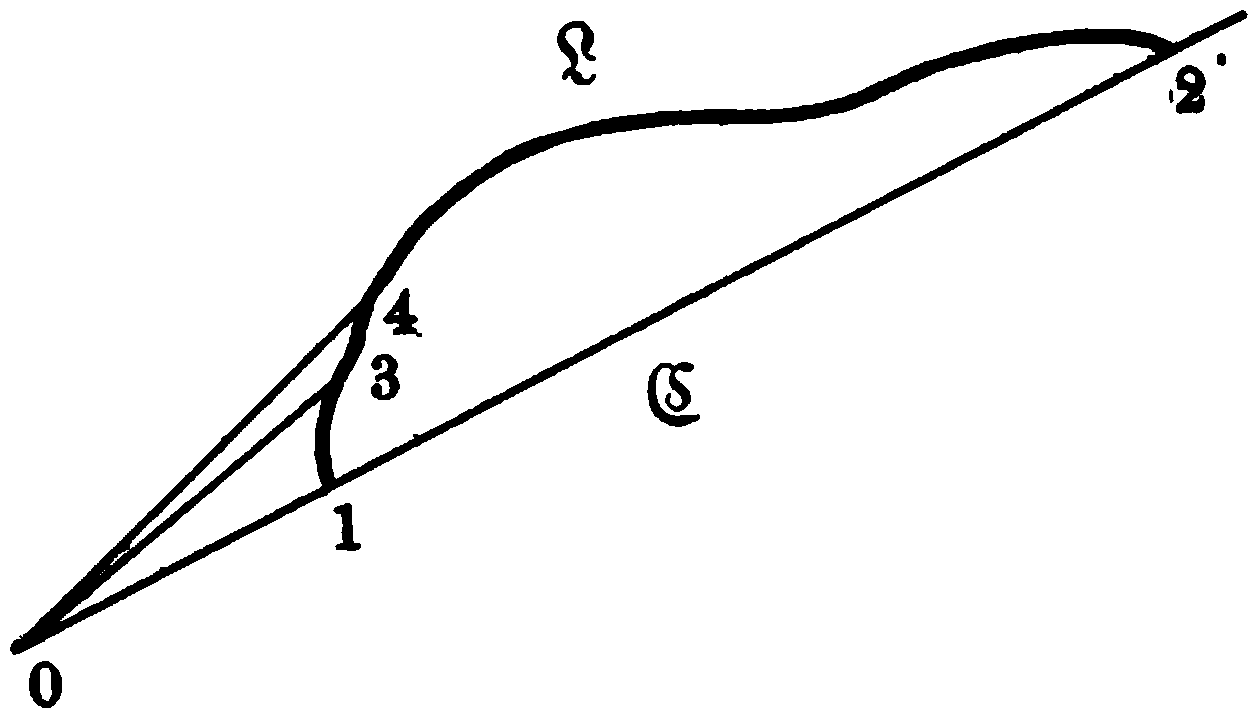
\includegraphics[width=\linewidth,height=30mm,keepaspectratio]{fig_assets/fig15_src_clean_x8.png}\par\vspace{1mm}
\end{minipage}
\end{center}

Thus if the point 4 lies sufficiently near 3 (Fig.~15), and if $\alpha$ is a sufficiently small prescribed value, then one can connect the points 0 and 4 by such an extremal of the field that the integral $\overline{K}_{04}$ formed along it has the value $\omega_3+\alpha$. Put in particular
\[
\alpha=K_{34},
\]
where the integral is formed along the curve $\Omega$; then all arguments of the expressions (13), and hence also the values of $a$ and $b$ obtained, are functions of $\tau$ of the kind denoted in \S~17 by $\varphi(\tau)$. There holds for the two extremals 03 and 04 the relation
\[
\overline{K}_{04}=\overline{K}_{03}+K_{34},
\]
and from this follows
\[
\overline{K}_{03}+K_{32}=\overline{K}_{04}+K_{42}.
\]
If, therefore, we allow the point 3 to pass into a neighboring position and connect it in that position with the point 0 by the defined extremal 03, then the quantity $\overline{K}_{03}+K_{32}$ remains constant. If in this manner we can let the point 3 traverse the whole arc $\Omega$
% src-pdfpage=0155
% src-break=0155
and if $\mathfrak{C}$ is the initial and final position of the constructed extremal 03, then we say that the \textsc{Weierstrass} construction is possible. The quantities $a,b$ belonging to the extremal 03 are then functions of $\tau$ throughout the whole interval from $\tau_1$ to $\tau_2$ with the properties of the quantities $\varphi(\tau)$ of \S~17; their initial and final values are $a_0,b_0$, while the constant quantity $\overline{K}_{03}+K_{32}$ assumes, for $\tau=\tau_1$ and $\tau=\tau_2$, the values
\[
\overline{K}_{01}+K_{12},
\quad
\overline{K}_{02}=\overline{K}_{01}+\overline{K}_{12},
\]
which are equal by (12). In special problems the \textsc{Weierstrass} construction can often be recognized as possible; a general condition for its practicability will be developed in \S~38.

In order now to come nearer to the question of the extremum of the integral $J$, we form, supposing the \textsc{Weierstrass} construction to be possible, the quantity
\[
W=\overline{J}_{03}+J_{32},
\]
where the first integral is formed along the constructed extremal 03, the second along the curve $\Omega$. This quantity is a function $\varphi(\tau)$ in the sense of \S~17, and since the extremal 03 finally passes into the position $\mathfrak{C}$, one has
\[
W\bigg|_{\tau_1}=\overline{J}_{01}+J_{12},
\quad
W\bigg|_{\tau_2}=\overline{J}_{01}+\overline{J}_{12}=\overline{J}_{02}.
\]
If it is therefore possible to prove the sign of the quantity $dW$ to be fixed, then the difference $\overline{J}_{12}-J_{12}$ is of the same sign. But the quantity $dW$ can be stated explicitly according to the formulae of \S~35; namely, since $\overline{K}_{03}+K_{32}$ is constant, and therefore
\[
\frac{d(\overline{K}_{03}+K_{32})}{d\tau}=0,
\]
one has
\[
\frac{dW}{d\tau}=\frac{d\overline{J}_{03}}{d\tau}+\lambda\frac{d\overline{K}_{03}}{d\tau}
+\frac{dJ_{32}}{d\tau}+\lambda\frac{dK_{32}}{d\tau},
\]
where $\lambda$ is the isoperimetric constant of the extremal 03. Using formula (11) and the evidently correct equations
\[
\frac{dJ_{32}}{d\tau}=-F\left(x,y,\frac{dx}{d\tau},\frac{dy}{d\tau}\right),
\quad
\frac{dK_{32}}{d\tau}=-G\left(x,y,\frac{dx}{d\tau},\frac{dy}{d\tau}\right)
\]
one obtains from this
% src-pdfpage=0156
% src-break=0156
\begin{equation}\tag{14}
\frac{dW}{d\tau}=H_{x'}(x,y,\xi_t,\eta_t)\frac{dx}{d\tau}
+H_{y'}(x,y,\xi_t,\eta_t)\frac{dy}{d\tau}
-H\left(x,y,\frac{dx}{d\tau},\frac{dy}{d\tau}\right).
\end{equation}
This expression is identical with the one earlier denoted by
\[
\frac{1}{d\tau}\mathfrak{E}(x,y,x',y',Dx,Dy)=
\mathfrak{E}\left(x,y,x',y',\frac{dx}{d\tau},\frac{dy}{d\tau}\right),
\]
in which $F$ is replaced by $H$; the properties of $\mathfrak{E}$ derived above (\S~21) can therefore be used, and in particular orderly and extraordinary vanishing can be distinguished. If $\mathfrak{E}$ always has a constant sign, and if it does not vanish everywhere along any of the curves $\Omega$ under consideration, then the required extremum of the integral $J$ is in fact furnished by the arc 12.

If $\mathfrak{E}$ vanished everywhere in an orderly manner along a finite part of the curve $\Omega$, then along that part one would have
\[
\frac{dx}{d\tau}=m\xi_t,
\quad
\frac{dy}{d\tau}=m\eta_t,
\quad
m>0;
\]
but since the equations
\[
x=\xi,
\quad
 y=\eta
\]
can also be differentiated with respect to $\tau$, one obtains
\begin{equation}\tag{15}
\begin{aligned}
\xi_t\frac{dt}{d\tau}+\xi_a\frac{da}{d\tau}+\xi_b\frac{db}{d\tau}&=m\xi_t,\\
\eta_t\frac{dt}{d\tau}+\eta_a\frac{da}{d\tau}+\eta_b\frac{db}{d\tau}&=m\eta_t.
\end{aligned}
\end{equation}
Further, evidently,
\[
\frac{d\omega}{d\tau}=\omega_t\frac{dt}{d\tau}+\omega_a\frac{da}{d\tau}+\omega_b\frac{db}{d\tau},
\quad
\omega_t=G(\xi,\eta,\xi_t,\eta_t);
\]
since $\overline{K}_{03}+K_{32}$ is independent of $\tau$, it follows that
\[
\frac{d\overline{K}_{03}}{d\tau}=-\frac{dK_{32}}{d\tau}=\frac{d\omega}{d\tau}=G\left(\xi,\eta,\frac{dx}{d\tau},\frac{dy}{d\tau}\right)
=mG(\xi,\eta,\xi_t,\eta_t)=m\omega_t,
\]
or
\[
\frac{d\omega}{d\tau}=\omega_t\frac{dt}{d\tau}+\omega_a\frac{da}{d\tau}+\omega_b\frac{db}{d\tau}=m\omega_t.
\]
This equation, together with those given under (15), can however be regarded as homogeneous linear equations in the quantities
% src-pdfpage=0157
% src-break=0157
\[
\frac{da}{d\tau},
\quad
\frac{db}{d\tau},
\quad
\frac{dt}{d\tau}-m.
\]
Since the determinant of the coefficients is identical with $\Delta$, and hence is different from zero, the three equations can hold together only if
\[
\frac{da}{d\tau}=\frac{db}{d\tau}=0.
\]
But from this, since $a$ and $b$ are determined by the \textsc{Weierstrass} construction as functions $\varphi(\tau)$ in the sense of \S~17, it would follow, if 3 and 4 are any two points of the arc considered, that
\[
a\bigg|_4^3=b\bigg|_4^3=0;
\]
the arc would therefore be a part of an extremal of the field. If $\mathfrak{E}$ vanished in an orderly manner along the whole curve $\Omega$, then, since $a_0,b_0$ are the final values of $a,b$, $\Omega$ would have to coincide with $\mathfrak{C}$. If this is not the case, and if an extraordinary vanishing of $\mathfrak{E}$, as well as a change of sign either altogether or by restriction of the compared curves $\Omega$, is excluded, then the difference
\[
W\bigg|_{\tau_1}^{\tau_2}=\int_{\tau_1}^{\tau_2}\mathfrak{E}\,d\tau=\overline{J}_{12}-J_{12}
\]
is different from zero and has its sign in common with $\mathfrak{E}$, by which the extremum is secured.

On the whole, then, three conditions have been proved sufficient for the occurrence of the extremum: 1) the existence of a field, or the \textsc{Jacobi} condition, 2) the \textsc{Weierstrass} sign condition, that is, the sign, fixed in the indicated sense, of the quantity $\mathfrak{E}$, 3) the possibility of the \textsc{Weierstrass} construction within the field. If these conditions are fulfilled, then the extremal $\mathfrak{C}$ furnishes an extremum of the integral $J_{12}$ in comparison with the curves 12 or $\Omega$ which run in the field and yield a prescribed value $K_{12}$. According as the sign of $\mathfrak{E}$ is secured altogether or only when $\Omega$ lies in a narrower neighborhood of the curve $\mathfrak{C}$, the extremum is strong or weak.

In general, however, the extremum is not furnished by the arc beginning at the point 0, but by the
% src-pdfpage=0158
% src-break=0158
arc 12, whose initial point 1 can move arbitrarily close to the position 0.

If, moreover, in the general investigation of \S~21 one replaces the function $F$ by $H$, one sees that the quantity $\mathfrak{E}$ considered here has a fixed sign as soon as the same is true of the quantity
\[
H_1=\frac{1}{y'^2}H_{x'x'}=\frac{1}{x'^2}H_{y'y'}=
\frac{1}{x'^2}(F_{y'y'}+\lambda G_{y'y'}),
\]
or also, if $x'$ does not vanish, of the product $(f_{pp}+\lambda g_{pp})dx$. The \textsc{Weierstrass} sign condition can therefore be replaced by the \textsc{Legendre} condition of \S~17 if in the latter one lets $F+\lambda G$ take the place of $F$.

If conditions 1) and 2) are fulfilled, then they remain fulfilled for the problem which one obtains by letting the integrals $J,K$ interchange their former roles. For condition 1) this follows immediately from the preceding remarks, according to which the property of certain extremals of forming a field is preserved under that interchange. The analogous result for condition 2) follows from the fact that $H$ and $\mathfrak{E}$ are replaced by
\[
G+\frac{1}{\lambda}F,
\quad
\frac{1}{\lambda}\mathfrak{E};
\]
the latter quantity evidently has, since $\lambda$ is different from zero, a fixed sign if this is true of $\mathfrak{E}$, although the sign need not be that of the quantity $\mathfrak{E}$. The extremum therefore has in the new problem the same character as in the old one, or the opposite character, according as $\lambda$ is positive or negative. Thus the simplest case of a reciprocity law established by \textsc{Mayer} has been proved.



% machine-unit: Kneser_LVR_EN_p0158low_p0177top §§37-39
% visible source begins below §37 on source pdfpage 0158; p0177 §40 heading/body excluded from this slice.

% src-pdfpage=0158
% src-break=0158
\begin{center}
{\large \S~37.}
\end{center}

\noindent\textbf{Example. Problem IX (\S~34).} The extremals are circles of radius $\pm\lambda$; those which pass through a point 0, for example the origin of coordinates, can be represented in the following way. Let $a,b$ be the coordinates of the centre $m$, and let the radius be $r$ (Fig.~16); then one may put
\begin{equation}\tag{16}
 x=a+r\cos\theta,\quad y=b+r\sin\theta,\quad r^2=a^2+b^2
\end{equation}
and $\theta$ is the angle through which the radius, starting from the position $mx$ parallel to the $+x$-axis, must be turned in the positive sense of rotation in order to bring its endpoint to the point 4 of the circle then under consideration; the positive sense is, as usual, the sense which, after a rotation through $90^\circ$, carries the
% src-pdfpage=0159
% src-break=0159
$+x$-axis into the $+y$-axis.

\begin{center}
\begin{minipage}{0.48\linewidth}\centering
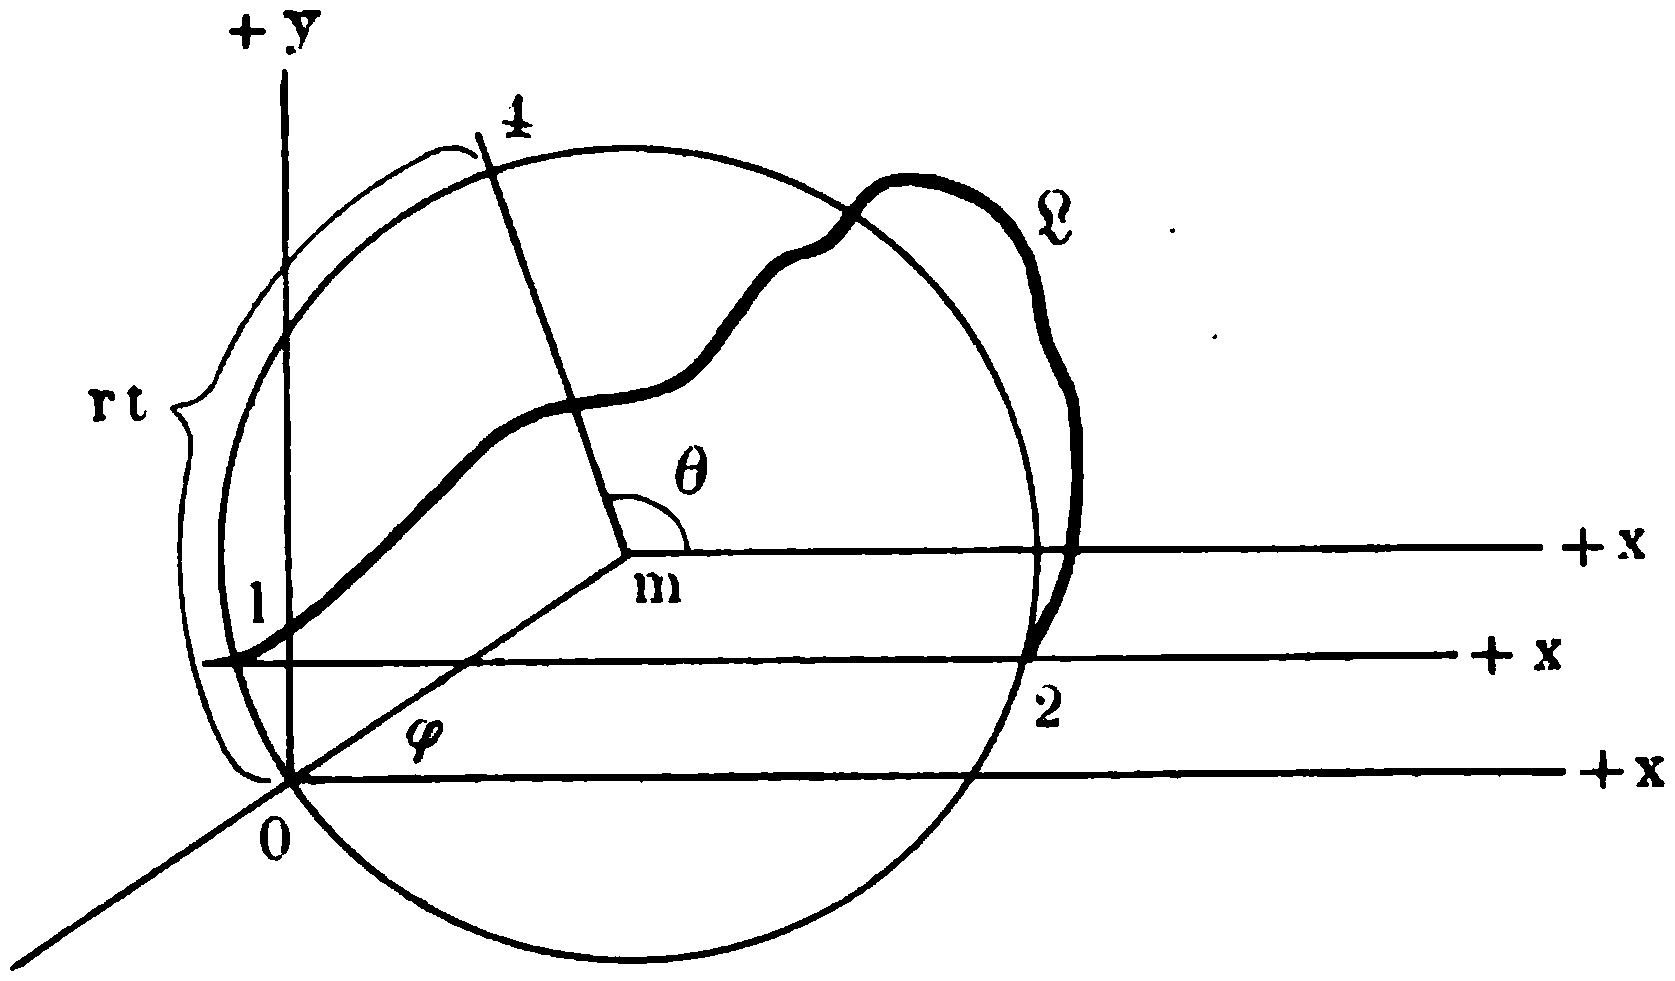
\includegraphics[width=\linewidth,height=36mm,keepaspectratio]{fig_assets/fig16_p0159_src_clean_x8.png}\par\vspace{1mm}
\end{minipage}
\end{center}

If, moreover, $\varphi$ is the angle by which the ray $0m$, measured in the positive sense, deviates from the $+x$-axis, then
\begin{equation}\tag{17}
 a=r\cos\varphi,\quad b=r\sin\varphi,
\end{equation}
and the radius $m0$ is therefore inclined by $\varphi+\pi$ with respect to $mx$. Hence, putting
\[
 t=\pi+\varphi-\theta,\quad \theta=\pi+\varphi-t,
\]
$rt$ is the circular arc 04 measured from the point 0 in the negative sense, and by (16), (17) one has
\[
 K_{04}=\omega=t\sqrt{a^2+b^2},\quad
 \xi(t,a,b)=a-a\cos t-b\sin t,
\]
\[
 \eta(t,a,b)=b-b\cos t+a\sin t.
\]
These functions are regular everywhere as long as $r$ remains between two otherwise quite arbitrary positive bounds. One has further
\[
\Delta=\begin{vmatrix}
1-\cos t&\sin t&\dfrac{at}{r}\\[1.0ex]
-\sin t&1-\cos t&\dfrac{bt}{r}\\[1.0ex]
a\sin t-b\cos t&a\cos t+b\sin t&r
\end{vmatrix},
\]
and if $a$ and $b$ are expressed by other variables $\alpha,\beta$,
\begin{equation}\tag{18}
\frac{\partial(\xi,\eta,\omega)}{\partial(t,\alpha,\beta)}=
\frac{\partial(\xi,\eta,\omega)}{\partial(t,a,b)}\cdot
\frac{\partial(t,a,b)}{\partial(t,\alpha,\beta)}
=\Delta\frac{\partial(a,b)}{\partial(\alpha,\beta)};
\end{equation}
if, in particular, $\alpha,\beta$ are the rectangular coordinates of the point $m$ in a new system, then the factor beside $\Delta$ has the value
% src-pdfpage=0160
% src-break=0160
$\pm1$. If now in particular $b=0$, then $a^2=r^2$, and
\[
\begin{aligned}
\Delta&=r\begin{vmatrix}
1-\cos t&\sin t&t\\
-\sin t&1-\cos t&0\\
\sin t&\cos t&1
\end{vmatrix}\\
&=r(2-2\cos t-t\sin t)=4r\sin\frac{t}{2}\left(\sin\frac{t}{2}-\frac{t}{2}\cos\frac{t}{2}\right).
\end{aligned}
\]
But if the point 4 traverses the circle under consideration, then $t$ moves in the interval
\begin{equation}\tag{19}
0\leq t<2\pi,
\end{equation}
and the factors of the expression $\Delta$ are therefore, apart from the point 0, different from zero. If $b$ does not vanish, replace the coordinate system $(a,b)$ by a new one $(\alpha,\beta)$ whose axis of abscissae passes through $m$; then, by formula (18), $\Delta$ likewise remains different from zero. Thus it is shown that all circles passing through the point 0 and subject, where $\varepsilon,\gamma$ denote positive constants, to the inequality
\begin{equation}\tag{20}
\varepsilon^2<a^2+b^2<\gamma^2
\end{equation}
form a field in the sense of \S~36 as soon as $t$ is restricted by (19), that is, as soon as none of the circles is regarded as traversed more than once.

Since in this problem
\[
F=yx',\quad G=\sqrt{x'^2+y'^2},\quad H=yx'+\lambda\sqrt{x'^2+y'^2},
\]
and the square roots are positive, one has
\[
\begin{aligned}
\mathfrak{E}&=\left(y+\frac{\lambda x'}{\sqrt{x'^2+y'^2}}\right)Dx+
\frac{\lambda y'}{\sqrt{x'^2+y'^2}}Dy-
\left(yDx+\lambda\sqrt{Dx^2+Dy^2}\right)\\
&=\lambda\sqrt{Dx^2+Dy^2}\left\{\frac{x'}{\sqrt{x'^2+y'^2}}\frac{Dx}{\sqrt{Dx^2+Dy^2}}+
\frac{y'}{\sqrt{x'^2+y'^2}}\frac{Dy}{\sqrt{Dx^2+Dy^2}}-1\right\};
\end{aligned}
\]
the quantity in brackets is (\S~23, Problem I) never positive, and $\mathfrak{E}$ vanishes only when
\[
\frac{x'}{\sqrt{x'^2+y'^2}}=\frac{Dx}{\sqrt{Dx^2+Dy^2}},\quad
\frac{y'}{\sqrt{x'^2+y'^2}}=\frac{Dy}{\sqrt{Dx^2+Dy^2}},
\]
that is, only in the ordinary way. Since, moreover, the direction of increasing $t$ lies with respect to the outward-directed radius as the
% src-pdfpage=0161
% src-break=0161
$+x$-axis lies with respect to the $+y$-axis, $\lambda$ is negative by \S~34, hence $\mathfrak{E}$ is positive, and the required extremum is a maximum.

Now let the points 1 and 2 be joined by an arc of a circle; outside this arc let the point 0 lie on the circle. Through this point draw the axis of abscissae parallel to the straight line 12, and place the $y$-axis so that $y$ is positive on this line. Then the direction of increasing $t$ defined above leads from 1 through the arc $\mathfrak{C}$ to the point 2, and the integral
\[
\overline{J}_{12}=\int_1^2 yx'\,dt
\]
is the positive area between $\mathfrak{C}$ and the straight segment 12, increased by the rectangle covered by the ordinates of the latter. Let $\Omega$ be an arbitrary curve joining 1 and 2, with the same continuity properties as in \S~17 and with the same length as $\mathfrak{C}$, which does not enter a circle with radius $2\varepsilon$ and centre 0; this can always be achieved by a suitable choice of that point. Then all circles which pass through 0 and a point 3 belonging to $\Omega$ have a radius greater than $\varepsilon$. If one restricts to those whose radii do not exceed a certain bound $\gamma$, they all belong to the field (20).

As the point 3 traverses the arc $\Omega$, join it in each of its positions to 0 by a circular arc of length
\[
\overline{K}_{01}+K_{13}=\operatorname{arc}01+\operatorname{arc}13,
\]
where the first arc is measured on the circle 012 and the second on the curve $\Omega$. This quantity is greater than the rectilinear distance 03; hence one obtains a finite radius for the required arc, and, since it evidently varies continuously with 3, a finite upper bound $\gamma$. Of the two circular arcs of the required kind which are symmetric with respect to the line 03 we always take the one which proceeds continuously from the initial position $\mathfrak{C}$; since the radius remains finite, $\mathfrak{C}$ is also the final position of the arc 03, and the Weierstrass construction within the field (20) is proved possible in its full extent. The general theory of \S~36 therefore gives
\[
\overline{J}_{12}>J_{12},
\]
that is, the segment bounded by the circular arc $\mathfrak{C}$ and the straight segment 12 is
% src-pdfpage=0162
% src-break=0162
greater than that defined by the curve $\Omega$. This is evidently still more than the maximum property.

\begin{center}
{\large \S~38.}
\end{center}

The Weierstrass construction can be carried out if one imposes on the curve $\Omega$ a restriction which appears natural in many problems, and which consists in requiring that, at neighboring points of the curves $\Omega$ and $\mathfrak{C}$, the integrals $K$ formed from the point 0 along both curves also differ only slightly from one another. To formulate this condition more precisely, suppose that an arbitrary curve issuing from the point 0 is traversed by the point 6, that $K_{06}$ is the integral obtained along this curve, and that $z$ is the third rectangular space-coordinate. Put generally
\[
x=x_6,\quad y=y_6,\quad z=K_{06},
\]
then the point $(x,y,z)$ describes a certain space curve, likewise issuing from the point 0; the points of space assigned in this way to any points $1,\ldots,6$ are denoted by $1^0,\ldots,6^0$. Each extremal of the field then corresponds to a curve
\[
x=\xi(t,a,b),\quad y=\eta(t,a,b),\quad z=\omega(t,a,b);
\]
for $a=a_0,b=b_0$ one obtains a space curve $\mathfrak{C}^0$ corresponding to the curve $\mathfrak{C}$. The line composed of the extremal arc 01 and the curve $\Omega$ corresponds to a space curve which coincides with $\mathfrak{C}^0$ up to the point $1^0$, whose coordinates are
\[
x=x_1,\quad y=y_1,\quad z=\overline{K}_{01}=\omega(t_1,a_0,b_0),
\]
and then separates from it; the point $3^0$ has the coordinates
\begin{equation}\tag{21}
x=x_3,\quad y=y_3,\quad z=\overline{K}_{01}+K_{13}.
\end{equation}
The new stipulation is that only those curves $\Omega$ are compared with $\mathfrak{C}$ with respect to the values of the integral $J$ whose corresponding space curves $\Omega^0$ belong to a certain neighborhood (\S~17) of the curve $\mathfrak{C}^0$.

On the latter, let the point $5^0$ correspond to a point 5 of the arc 12, for which
\[
x=x_5,\quad y=y_5,\quad z=\overline{K}_{05}=\omega(t_5,a_0,b_0)=z_5;
\]
then the equations
% src-pdfpage=0163
% src-break=0163
\begin{equation}\tag{22}
\begin{aligned}
x-x_5&=\xi(t,a,b)-x_5=[t-t_5,a-a_0,b-b_0]_1,\\
y-y_5&=\eta(t,a,b)-y_5=[t-t_5,a-a_0,b-b_0]_1,\\
z-z_5&=\omega(t,a,b)-z_5=[t-t_5,a-a_0,b-b_0]_1
\end{aligned}
\end{equation}
in which the linear terms on the right have the determinant $\Delta(t_5,a_0,b_0)$, can be satisfied by inserting for $t-t_5,a-a_0,b-b_0$ certain determinate series of the form
\[
[x-x_5,\ y-y_5,\ z-z_5]_1.
\]
These expressions define $t,a,b$ as functions of $x,y,z$ which are regular at every point $5^0$; hence, if the curve $\mathfrak{C}$ does not intersect itself, so that different values $t_5$ also correspond to different points $5^0$, they are regular and uniquely determined within a certain domain $\mathfrak{G}^0$ containing the arc $1^02^0$, so that this domain is filled simply by the extremals corresponding to the $a,b$ defined by the preceding expressions. If the point under consideration falls on the curve $\mathfrak{C}^0$ itself, then $a$ and $b$ pass into $a_0$ and $b_0$. The domain $\mathfrak{G}^0$ may be pictured, for example, as the space swept out by a sphere of constant radius whose centre traverses the arc $1^02^0$.

If now the curve $\Omega^0$ lies wholly in the interior of $\mathfrak{G}^0$, then each point $3^0$ lies on a definite one of the extremals of the field, and one has
\[
x_3=\xi(t_3,a,b),\quad y_3=\eta(t_3,a,b),\quad z_3=\omega(t_3,a,b).
\]
It follows from the third equation (21) that
\[
\omega(t_3,a,b)=\overline{K}_{03}=\overline{K}_{01}+K_{13},
\]
and therefore
\[
\overline{K}_{03}+K_{32}=\overline{K}_{01}+K_{13}+K_{32}=\overline{K}_{01}+K_{12}=\overline{K}_{02};
\]
the projection of the constructed curve $03^0$ onto the $xy$-plane is thus exactly the extremal 03 sought in the Weierstrass construction, and, by the remarks attached to equations (22), it passes into $\mathfrak{C}$ when the point $3^0$ moves into one of the positions $1^0$ and $2^0$. Under the newly introduced restriction on the curves $\Omega$, the Weierstrass construction is therefore always possible, and one of the sufficient conditions for the extremum stated in \S~36 disappears.

\noindent\textbf{Example. Problem XI.} To place a heavy homogeneous string of given length and given endpoints in a vertical plane so that its centre of gravity lies as low as possible (equilibrium figure, catenary).
% src-pdfpage=0164
% src-break=0164
If the $+y$-axis is the direction of gravity, $l$ the length of the string 01, and the mass per unit length is one, then the ordinate of the centre of gravity is
\[
\frac{1}{l}\int_0^1 y\sqrt{x'^2+y'^2}\,dt,
\]
so the integral
\[
J=\int_0^1 y\sqrt{x'^2+y'^2}\,dt
\]
is to be made a maximum subject to a prescribed value of the arc-length integral
\[
K=\int_0^1 \sqrt{x'^2+y'^2}\,dt,
\]
and the first variation of the integral
\[
J+\lambda K=\int (y+\lambda)\sqrt{x'^2+y'^2}\,dt
\]
is to be set equal to zero. For the extremals one obtains from this (\S~9, Problem II) the equation
\[
y+\lambda=\frac{a}{2}\left\{e^{\frac{x-b}{a}}+e^{-\frac{x-b}{a}}\right\}=a\Cof\frac{x-b}{a}.
\]
For $x=\pm\infty$ the right-hand side has the sign of the quantity $a$; the curve is therefore convex downward for $a<0$. Then $y+\lambda$ is always negative, and the quantity
\[
\mathfrak{E}=(y+\lambda)\sqrt{Dx^2+Dy^2}\left\{\frac{x'Dx+y'Dy}{\sqrt{x'^2+y'^2}\sqrt{Dx^2+Dy^2}}-1\right\}
\]
is positive, and is equal to zero only when the systems of values $(x',y')$ and $(Dx,Dy)$ represent the same direction. Thus the Weierstrass sign condition for the strong maximum is satisfied.

The further calculation is simplified by means of the easily proved formulae
\begin{equation}\tag{23}
\begin{aligned}
\Cof(u+v)&=\Cof u\Cof v+\Sin u\Sin v,\\
\Sin(u+v)&=\Sin u\Cof v+\Sin v\Cof u.
\end{aligned}
\end{equation}
For the constants of the extremals passing through the fixed point 0 one has the relation
\[
y_0+\lambda=a\Cof\frac{x_0-b}{a},
\]
% src-pdfpage=0165
% src-break=0165
and the general equation of this family of curves can accordingly be written
\[
y-y_0=a\left\{\Cof\frac{x-b}{a}-\Cof\frac{x_0-b}{a}\right\}.
\]
The right-hand side of this equation is regular as soon as $a$ is different from zero, and one may put
\[
x=\xi(t,a,b)=t,\quad y=\eta(t,a,b)=y_0+a\left\{\Cof\frac{t-b}{a}-\Cof\frac{t_0-b}{a}\right\}.
\]
Since
\[
\xi_t=1,\quad \xi_a=\xi_b=0,
\]
one has
\[
\Delta(t,a,b)=\frac{\partial(\xi,\eta,\omega)}{\partial(t,a,b)}=\frac{\partial(\eta,\omega)}{\partial(a,b)}.
\]
Moreover $\omega$ is the arc length measured from the point 0, hence
\[
\omega=\int_0^t\sqrt{1+y'^2}\,dt=\int_0^t\sqrt{1+\Sin^2\frac{t-b}{a}}\,dt
=\int_0^t \Cof\frac{t-b}{a}\,dt,
\]
\[
=a\left\{\Sin\frac{t-b}{a}-\Sin\frac{t_0-b}{a}\right\};
\]
therefore, putting
\[
\frac{t-b}{a}=u,
\quad
\frac{t_0-b}{a}=u_0,
\]
one obtains, on the basis of the formulae for the differentials of the hyperbolic functions (\S~23),
\[
-\Delta=\begin{vmatrix}
\Cof u-\Cof u_0-(u\Sin u-u_0\Sin u_0)&\Sin u-\Sin u_0\\
\Sin u-\Sin u_0-(u\Cof u-u_0\Cof u_0)&\Cof u-\Cof u_0
\end{vmatrix};
\]
if this is further differentiated and equations (23) are used, it follows that
\[
\begin{aligned}
-\frac{d\Delta}{du}&=\begin{vmatrix}
-u\Cof u&\Sin u-\Sin u_0\\
-u\Sin u&\Cof u-\Cof u_0
\end{vmatrix}
+\begin{vmatrix}
\Cof u-u\Sin u-\Cof u_0+u_0\Sin u_0&\Cof u\\
\Sin u-u\Cof u-\Sin u_0+u_0\Cof u_0&\Sin u
\end{vmatrix}\\
&=(u-u_0)\Cof(u-u_0)-\Sin(u-u_0).
\end{aligned}
\]
Hence
\[
-\frac{d^2\Delta}{du^2}=(u-u_0)\Sin(u-u_0);
\]
since $u-u_0$ and $\Sin(u-u_0)$ have the same sign, one always has
% src-pdfpage=0166
% src-break=0166
\[
\frac{d^2\Delta}{du^2}\leq0;
\]
and since $\Delta$ and $d\Delta:du$ vanish for $u=u_0$, the latter always has the sign of $u_0-u$, and the former is negative as soon as $u\gtrless u_0$. If, starting from the point 0, one follows the catenary in the direction of increasing $x$, then
\[
u-u_0=\frac{x-x_0}{a}
\]
is negative, like $a$, and hence $\Delta$ is negative; therefore, for an arbitrarily long piece of the downward-convex catenary, the sufficient conditions for the strong maximum are satisfied under the above restriction on the curves $\Omega$. In accordance with a remark made in \S~36, the maximum is thereby first obtained for every arc 12 whose initial point lies arbitrarily close to 0; since the position of the latter is subject to no restriction, the arc 12 may be regarded as an arbitrary part of the curve.

The introduced restriction on the curve $\Omega$ appears natural here, because under every small displacement of a string the individual material point, which is defined by a definite length of string measured from the point 0, is imagined as displaced only slightly. The curves $\Omega$ and $\mathfrak{C}$ are then placed in one-to-one correspondence in such a way that corresponding points have small distance and give the same value of the integral $K$.

\begin{center}
{\large \S~39.}
\end{center}

The general developments of the preceding paragraphs remain valid, with minor modifications, if one assumes that the extremals
\begin{equation}\tag{24}
x=\xi(t,a,b),\quad y=\eta(t,a,b),
\end{equation}
to which $\mathfrak{C}$ belongs do not pass through a fixed point 0, but all cut a fixed curve $\mathfrak{C}_0$ transversally; one then obtains criteria for a piece of the curve $\mathfrak{C}$ to furnish an extremum of the integral among all curves joining a fixed point to the curve $\mathfrak{C}_0$ and giving the integral $K$ a prescribed value.

Let
\[
\Gamma(x,y)=0
\]
% src-pdfpage=0167
% src-break=0167
be the equation of the curve $\mathfrak{C}_0$; let it cut $\mathfrak{C}$ and the curves of the family (24) differing sufficiently little from it at the variable point 0 under non-vanishing angles, and let it be regular at this point. Then one has the equation
\begin{equation}\tag{25}
\Gamma[\xi(t_0,a,b),\eta(t_0,a,b)]=0,
\end{equation}
which can be solved for $t_0$, since at the points 0 under consideration the inequality
\[
\Gamma_x\xi_t+\Gamma_y\eta_t\neq0
\]
holds. Thus, if $t_{00}$ is the parameter which on the curve $\mathfrak{C}$ belongs to its point of intersection with $\mathfrak{C}_0$,
\[
t_0-t_{00}=[a-a_0,b-b_0]_1.
\]
Since, moreover, the extremals of the family (24) cut the curve $\mathfrak{C}_0$ transversally, under the assumption
\[
\left.\Gamma_xDx+\Gamma_yDy\right|^0=0
\]
one always obtains the equation
\[
\left.H_{x'}Dx+H_{y'}Dy\right|^0=0;
\]
therefore
\begin{equation}\tag{26}
\left.\Delta=H_{x'}\Gamma_y-H_{y'}\Gamma_x\right|^0=0,
\end{equation}
where the arguments
\begin{equation}\tag{27}
x=\xi,\quad y=\eta,\quad x'=\xi_t,\quad y'=\eta_t
\end{equation}
are to be taken. If equation (25) is then differentiated with respect to $a$ and $b$, one obtains
\[
\left.\Gamma_x\left(\xi_t\frac{\partial t_0}{\partial a}+\xi_a\right)+\Gamma_y\left(\eta_t\frac{\partial t_0}{\partial a}+\eta_a\right)\right|^0=0,
\]
\[
\left.\Gamma_x\left(\xi_t\frac{\partial t_0}{\partial b}+\xi_b\right)+\Gamma_y\left(\eta_t\frac{\partial t_0}{\partial b}+\eta_b\right)\right|^0=0.
\]
In these equations one may, by (26), replace $\Gamma_x$ and $\Gamma_y$ by $H_{x'}$ and $H_{y'}$; they then become exactly identical with formulae (9). If, therefore, along any extremal of the family to which the variable point 3 belongs, one forms the integrals
\[
\overline{J}_{03}=\int_0^3 F\,dt=\int_{t_0}^{t}F(\xi,\eta,\xi_t,\eta_t)\,dt,\quad
\overline{K}_{03}=\int_{t_0}^{t}G(\xi,\ldots,\eta_t)\,dt,
\]
then first of all equation (7), independent of the connection between $t_0,a,b$, still holds, and from it there follow
% src-pdfpage=0168
% src-break=0168
exactly as in \S~35, on the basis of formula (9), equations (10), (11).

Now put, as above,
\[
\overline{K}_{03}=\omega(t,a,b)
\]
and assume that the determinant
\[
\Delta=\frac{\partial(\xi,\eta,\omega)}{\partial(t,a,b)}
\]
does not vanish along the arc 02 belonging to the curve $\mathfrak{C}$, except at the point 0; then the same is true for all arcs of extremals of the family beginning on the curve $\mathfrak{C}_0$ which differ sufficiently little from 02. The totality of the arcs for which $\Delta$ remains different from zero is called the field of the arc 02. On the curve $\mathfrak{C}_0$ itself $\Delta$ vanishes everywhere, as is easily seen from formulae (7), (9). A certain neighborhood of the arc 02 is then, as a consideration carried out in \S~35 also now shows, in general covered infinitely many times by the extremals of the field. Inside this neighborhood, let a point 1 belonging to the curve $\mathfrak{C}_0$ be joined to 2 by a line $\Omega$ for which
\begin{equation}\tag{28}
K_{12}=\overline{K}_{02}
\end{equation}
holds, the integral on the right being taken along the curve $\mathfrak{C}$, while the unbarred integrals are, here as always, to refer to the curve $\Omega$. Let this curve be traversed by the point 3. A construction analogous to Weierstrass's then consists in constructing an extremal of the field, varying with 3, for which $\overline{K}_{03}+K_{32}$ remains constant and which, when the points 3 and 2 coincide, passes into the curve $\mathfrak{C}$. The initial and final values of this quantity are then plainly the two sides of equation (28).

The proof given in \S~38 for the possibility of the Weierstrass construction, however, cannot be transferred without further modification to the present problem, since $\Delta$ vanishes on the curve $\mathfrak{C}_0$, as noted. This circumstance has no influence on the argument of \S~36, according to which $\mathfrak{E}$ can vanish everywhere in the ordinary way only along an extremal of the field; since now the quantity $\overline{K}_{03}+K_{32}$ is independent of $\tau$, and since, moreover, equations (7), (10), (11) of \S~35 also hold here, as has been shown, one obtains, as in \S~36:
% src-pdfpage=0169
% src-break=0169
\[
\frac{dW}{d\tau}=\frac{d(\overline{J}_{03}+J_{32})}{d\tau}
=H_x\frac{dx}{d\tau}+H_y\frac{dy}{d\tau}-H\left(x,y,\frac{dx}{d\tau},\frac{dy}{d\tau}\right)
=\mathfrak{E}\left(x,y,x',y',\frac{dx}{d\tau},\frac{dy}{d\tau}\right).
\]
The initial and final values of the quantity $W$ are different from the former ones; one plainly now has
\[
\left.W\right|^{\tau_1}=J_{12},\quad \left.W\right|^{\tau_2}=\overline{J}_{02};
\]
therefore the difference $\overline{J}_{02}-J_{12}$ has the sign of the quantity $\mathfrak{E}$.

If, therefore, the extremals of the field cut the regular curve $\mathfrak{C}_0$ transversally without touching it, then the sufficient conditions for the extremum stated in \S~36 have the same meaning for the extremum among all lines $\Omega$ joining the curve $\mathfrak{C}_0$ to a fixed point.

\noindent\textbf{Examples. Problem IX} is specialized in the following way. From a point 2 let an arbitrary fixed curve $\mathfrak{F}$ be drawn to a circle $\mathfrak{C}_0$; join the point 2 to the same circle $\mathfrak{C}_0$ by a second curve of given length, which with this circle and the curve $\mathfrak{F}$ encloses as large an area as possible.

\begin{center}
\begin{minipage}{0.45\linewidth}\centering
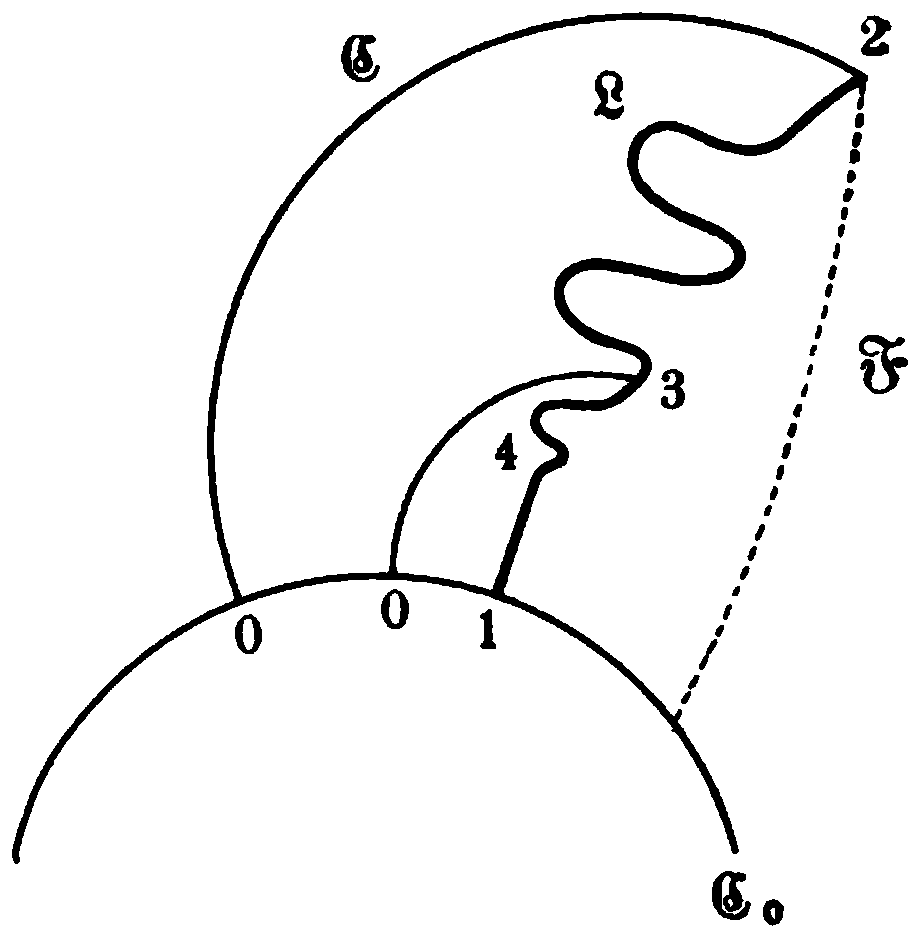
\includegraphics[width=\linewidth,height=42mm,keepaspectratio]{fig_assets/fig17_p0169_src_clean_x8.png}\par\vspace{1mm}
\end{minipage}
\end{center}

The extremals are circles (Fig.~17) and, by \S~34, lie transversally to the circle $\mathfrak{C}_0$ when they cut it orthogonally. Since every point 3 can be joined to the circle $\mathfrak{C}_0$ by a circular arc 03 orthogonal to it and of prescribed length, as soon as this length exceeds the shortest straight connecting segment between the point and $\mathfrak{C}_0$, the Weierstrass construction is always possible along any arc $\Omega$ or 12 of the prescribed length in such a way that the arc 03 is equal to the arc 13 measured along the curve $\Omega$; in this, the circular arcs 03 can be chosen so that a point traversing the circle $\mathfrak{C}_0$ in a definite direction $\mathfrak{R}$ goes at every position 0 toward the concave side of the arc 03. This construction, however, is to be carried out only for a
% src-pdfpage=0170
% src-break=0170
piece 42 of the arc $\Omega$, if that arc begins with the straight segment 14 normal to the circle $\mathfrak{C}_0$, but leaves the line 14 at the point 4; then the segment 14 is the limiting position of the arcs 03 when 3 and 4 are made to approach one another, so that
\begin{equation}\tag{29}
\left.\overline{J}_{03}+J_{32}\right|^{\tau_4}=J_{12},\quad
\left.\overline{K}_{03}+K_{32}\right|^{\tau_4}=K_{12}
\end{equation}
can be put. Moreover, when the point 3 moves into the position 2, the limiting position of the arc 03 is the arc $\mathfrak{C}$, or 02, with which $\Omega$ is compared; hence the equation
\[
\lim \overline{J}_{03}=\overline{J}_{02}
\]
holds, and by (29)
\[
\left.\overline{J}_{03}+J_{32}\right|_{\tau_4}^{\tau_2}=\int_{\tau_4}^{\tau_2}\mathfrak{E}\,d\tau=\overline{J}_{02}-J_{12}.
\]
Since $\mathfrak{E}$ has a fixed sign, the extremum follows as long as Jacobi's condition is fulfilled.

To see in what range this is the case, suppose that
\[
x_0^2+y_0^2=r^2
\]
is the equation of the circle $\mathfrak{C}_0$; if $b$ is the arc length increasing in the direction $\mathfrak{R}$, then
\[
\alpha=x_0+a\frac{dx_0}{db},\quad \beta=y_0+a\frac{dy_0}{db}
\]
are the coordinates of the centre of an arc 03 of radius $|a|$; in view of the meaning of $\mathfrak{R}$, $a$ is positive. According to the mode of representation used in \S~37, the circular arc 03, after replacing the coordinate origin by the point 0, can be represented by the following equations:
\[
\begin{aligned}
x-x_0&=(\alpha-x_0)-(\alpha-x_0)\cos t-(\beta-y_0)\sin t,\\
y-y_0&=(\beta-y_0)+(\alpha-x_0)\sin t-(\beta-y_0)\cos t,
\end{aligned}
\]
or, putting
\[
\xi(t,a,b)=x_0+a\frac{dx_0}{db}-a\frac{dx_0}{db}\cos t-a\frac{dy_0}{db}\sin t,
\]
\[
\eta(t,a,b)=y_0+a\frac{dy_0}{db}+a\frac{dx_0}{db}\sin t-a\frac{dy_0}{db}\cos t,
\]
by the equations
\[
x=\xi(t,a,b),\quad y=\eta(t,a,b).
\]
Plainly $t=0$ at the point 0; therefore
\[
\overline{K}_{03}=at=\omega(t,a,b),
\]
% src-pdfpage=0171
% src-break=0171
\begingroup
\setlength{\arraycolsep}{1pt}
\[
\Delta=\frac{\partial(\xi,\eta,\omega)}{\partial(t,a,b)}=
\begin{vmatrix}
 a\dfrac{dx_0}{db}\sin t-a\dfrac{dy_0}{db}\cos t & a\dfrac{dx_0}{db}\cos t+a\dfrac{dy_0}{db}\sin t & a\\[1.0ex]
 \dfrac{dx_0}{db}(1-\cos t)-\dfrac{dy_0}{db}\sin t & \dfrac{dy_0}{db}(1-\cos t)+\dfrac{dx_0}{db}\sin t & t\\[1.0ex]
 \dfrac{dx_0}{db}+a\dfrac{d^2x_0}{db^2}(1-\cos t)-a\dfrac{d^2y_0}{db^2}\sin t & \dfrac{dy_0}{db}+a\dfrac{d^2y_0}{db^2}(1-\cos t)+a\dfrac{d^2x_0}{db^2}\sin t & 0
\end{vmatrix}.
\]
\endgroup
If now, for the arc 03 under consideration, the equations
\begin{equation}\tag{30}
\frac{dy_0}{db}=0,\quad \frac{dx_0}{db}=1
\end{equation}
hold, then the identity
\[
\frac{dy_0}{db}\frac{d^2y_0}{db^2}+\frac{dx_0}{db}\frac{d^2x_0}{db^2}=0
\]
at once gives
\[
\frac{d^2x_0}{db^2}=0;
\]
therefore one obtains
\[
\Delta=-a(\sin t-t\cos t)+a^2\frac{d^2y_0}{db^2}\begin{vmatrix}
\sin t&\cos t&1\\
1-\cos t&\sin t&t\\
-\sin t&1-\cos t&0
\end{vmatrix},
\]
and with the notation
\[
\varphi(t)=\sin t-t\cos t
\]
it follows that
\[
\Delta=-a\varphi(t)+4a^2\frac{d^2y_0}{db^2}\sin\frac{t}{2}\,\varphi\left(\frac{t}{2}\right).
\]
Furthermore, along the circle $\mathfrak{C}_0$ one plainly has
\[
x_0=r\cos\frac{b}{r},\quad y_0=r\sin\frac{b}{r};
\]
and if for the point 0 the assumption
\[
b=\frac{3r\pi}{2}
\]
is made, equations (30) hold and therefore so do the following:
% src-pdfpage=0172
% src-break=0172
\[
\frac{d^2y_0}{db^2}=-\frac{1}{r}\sin\frac{b}{r}=\frac{1}{r},
\]
\[
\Delta=-\frac{a}{r}\left\{r\varphi(t)-4a\sin\frac{t}{2}\,\varphi\left(\frac{t}{2}\right)\right\}.
\]
Thus, as long as the circular arcs 03, measured in parts of the radius $a$, do not reach the smallest root of the equation
\[
r\varphi(t)-4a\sin\frac{t}{2}\,\varphi\left(\frac{t}{2}\right)=0,
\]
the arc 02 really supplies an extremum of the area enclosed by it, the circle $\mathfrak{C}_0$, and a fixed line joining the latter to 2.

It is easy to see that this result remains valid if $\mathfrak{C}_0$ is an arbitrary regular curve and $r$ is its radius of curvature at the point where it is cut orthogonally by the circular arc 03.

\noindent\textbf{Problem XI (\S~38).} To investigate the stability of a heavy string when one endpoint is fixed and the other is movable on a given curve.

We start from the following general remark. Let a two-parameter family of extremals, which either pass through a point 0 or cut the curve $\mathfrak{C}_0$ transversally, be given by the equations
\[
x=\xi(t,a,b,c),\quad y=\eta(t,a,b,c),
\]
\[
\overline{K}_{03}=\omega=\omega(t,a,b,c),\quad g(a,b,c)=0,
\]
where $g_c$ is different from zero; then the quantity $\Delta$ has the following form:
\begingroup
\setlength{\arraycolsep}{1pt}
\[
\Delta=\frac{\partial(\xi,\eta,\omega)}{\partial(t,a,b)}=
\begin{vmatrix}
\xi_t&\xi_a+\xi_c\dfrac{\partial c}{\partial a}&\xi_b+\xi_c\dfrac{\partial c}{\partial b}\\[1.0ex]
\eta_t&\eta_a+\eta_c\dfrac{\partial c}{\partial a}&\eta_b+\eta_c\dfrac{\partial c}{\partial b}\\[1.0ex]
\omega_t&\omega_a+\omega_c\dfrac{\partial c}{\partial a}&\omega_b+\omega_c\dfrac{\partial c}{\partial b}
\end{vmatrix},
\]
and since evidently
\[
g_a+g_c\frac{\partial c}{\partial a}=g_b+g_c\frac{\partial c}{\partial b}=0,
\]
one obtains
% src-pdfpage=0173
% src-break=0173
\[
\Delta g_c^2=\begin{vmatrix}
\xi_t&\xi_ag_c-\xi_cg_a&\xi_bg_c-\xi_cg_b\\
\eta_t&\eta_ag_c-\eta_cg_a&\eta_bg_c-\eta_cg_b\\
\omega_t&\omega_ag_c-\omega_cg_a&\omega_bg_c-\omega_cg_b
\end{vmatrix}
=g_c\begin{vmatrix}
\xi_t&\xi_a&\xi_b&\xi_c\\
\eta_t&\eta_a&\eta_b&\eta_c\\
\omega_t&\omega_a&\omega_b&\omega_c\\
0&g_a&g_b&g_c
\end{vmatrix},
\]
\endgroup
so that $g_c\Delta$ is equal to the determinant of fourth order standing on the right.

Let the given curve $\mathfrak{C}_0$ now have the equation
\[
y_0=f(x_0);
\]
at the place under consideration let it not be horizontal, so that $f'(x_0)$ is different from zero. The extremals for which
\[
y+\lambda=a\Cof\frac{x-b}{a},\quad p=\Sin\frac{x-b}{a}
\]
must be cut orthogonally by $\mathfrak{C}_0$ at the point 0, if 0 is the movable endpoint of the string; hence one has the equations
\begin{equation}\tag{31}
\begin{aligned}
y_0+\lambda&=a\Cof\frac{x_0-b}{a},\\
1+f'(x_0)p_0&=1+f'(x_0)\Sin\frac{x_0-b}{a}=0,
\end{aligned}
\end{equation}
and the whole family of transversally cutting extremals is defined, putting $-x=t$ and denoting by $\omega$ the length measured from the point 0 in the sense of decreasing $x$, by
\[
x=-t,\quad y=f(x_0)+a\left(\Cof\frac{x-b}{a}-\Cof\frac{x_0-b}{a}\right),
\]
\[
\omega=-a\left(\Sin\frac{x-b}{a}-\Sin\frac{x_0-b}{a}\right),\quad
0=1+f'(x_0)\Sin\frac{x_0-b}{a}.
\]
The quantity $-\Delta$, multiplied by the analogue of the quantity denoted above by $g_c$, is therefore the functional determinant of the right sides of the last three equations with respect to $a,b,x_0$; putting
\[
\frac{x-b}{a}=u,
\quad
\frac{x_0-b}{a}=u_0,
\]
one finds immediately, from the addition formulae for the functions $\Sin,\Cof$,
\[
\Delta=-\Phi(u)+\frac{1}{a}\Ctg^2u_0\,\Phi'(u)\left[f''(x_0)\Sin u_0-\frac{1}{a}\Ctg u_0\right]^{-1},
\]
where
% src-pdfpage=0174
% src-break=0174
\[
\Phi(u)=2-2\Cof(u-u_0)+(u-u_0)\Sin(u-u_0).
\]
For this function the equations
\[
\Phi(u_0)=\Phi'(u_0)=0,\quad \Phi''(u)=(u-u_0)\Sin(u-u_0)
\]
\[
\Phi(u)\Phi''(u)-[\Phi'(u)]^2=[\Phi(u)]^2\frac{d}{du}\left[\frac{\Phi'(u)}{\Phi(u)}\right]
= -[u-u_0-\Sin(u-u_0)]^2,
\]
\[
\frac{\Phi'(u)}{\Phi(u)}=\frac{u-u_0-\Tg(u-u_0)}{(u-u_0)\Tg(u-u_0)-2+[2:\Cof(u-u_0)]}
\]
hold; from them it follows immediately that for $u>u_0$ the quantities $\Phi(u)$ and $\Phi'(u)$ are always positive, but that the quotient $\Phi'(u):\Phi(u)$, as $u$ starts from $u_0$ and tends to positive infinity, traverses the interval from $+\infty$ to $+1$ steadily decreasing.

Now consider only equilibrium positions for which Legendre's condition for the maximum of the ordinate of the centre of gravity is fulfilled. Then the extremals under consideration must be convex downward; hence, since $+y$ is the direction of gravity, $a<0$. The equation
\begin{equation}\tag{32}
\Delta=0,
\quad
\frac{\Phi'(u)}{\Phi(u)}=\Tg u_0\left[\frac{a f''(x_0)\Sin^2u_0}{\Cof u_0}-1\right]
\end{equation}
therefore has, when $\Sin u_0$ and hence $\Tg u_0$, as well as $f''(x_0)$, is positive, no root above the value $u_0$. The same is also true, since the equation can be written
\[
\Cof u_0\left[\Ctg u_0\frac{\Phi'(u)}{\Phi(u)}+1\right]=a f''(x_0)\Sin^2u_0,
\]
when $\Sin u_0$ is negative and $f''(x_0)$ is not positive; for then
\[
\Ctg u_0<-1,
\]
so the left-hand side of the last equation is certainly negative for $u>u_0$, whereas the right-hand side is positive or zero. Now by (31) the quantities $\Sin u_0$ and $f'(x_0)$ have opposite signs; in the two cases considered, therefore, $f'(x_0)$ and $f''(x_0)$ have opposite signs, so that the direction of decreasing $x$, or, since $a$ is negative, of increasing $u$, points toward the convex side of the curve $\mathfrak{C}_0$. Jacobi's condition for the stability of the equilibrium is therefore always fulfilled when the string at the point 0 goes toward the convex side of the curve $\mathfrak{C}_0$, or when this curve has zero curvature at the point 0, for example when it is a straight line. If in one of these cases the Weierstrass
% src-pdfpage=0175
% src-break=0175
construction is possible, then all arcs 03 lie in the interior of the field, and the stability is secured for an arbitrarily long piece of the string.

If $f''(x_0)$ and $f'(x_0)$ have the same sign, so that the string, for which $u>u_0$, goes toward the concave side of the curve $\mathfrak{C}_0$, then equation (32) has for $u>u_0$ a single root $\bar u$, as soon as the inequality
\[
\Tg u_0\left[\frac{a f''(x_0)\Sin^2u_0}{\Cof u_0}-1\right]>1
\]
holds. Thus, if the direction of the curve $\mathfrak{C}_0$ and the shape of the string, that is, the quantities $a$ and $u_0$, are regarded as fixed, and the curvature of the curve $\mathfrak{C}_0$ is varied, a root $\bar u$ appears as soon as the absolute value of the curvature has reached a certain limit. If this absolute value grows beyond all bounds, then $\bar u$ approaches the limit $u_0$ steadily decreasing; that is, the piece of the string for which Jacobi's condition is fulfilled becomes infinitely small.

To discuss the Weierstrass construction, we now seek a catenary which at the point 0 touches the fixed straight line $T$, lying neither horizontally nor vertically, and also contains the point 1, which does not lie on the same vertical as 0. The equation of the straight line $T$ can be written
\[
y-y_0=(x-x_0)\Sin u_0;
\]
the value $u_0$ is then uniquely determined, since the function $\Sin$, as its argument increases, takes all values from $-\infty$ to $+\infty$ increasingly. All catenaries touching the line $T$ at the point 0 are represented by the equations
\begin{equation}\tag{33}
y-y_0=a(\Cof u-\Cof u_0),\quad x=x_0+a(u-u_0),
\end{equation}
in which $u$ is a parameter. If we regard $a$ as variable and $x$ as fixed, then
\[
\frac{\partial y}{\partial a}=\Cof u+a\Sin u\frac{\partial u}{\partial a}-\Cof u_0
=\Cof u-(u-u_0)\Sin u-\Cof u_0;
\]
the derivative of the right-hand side with respect to $u$ is $(u_0-u)\Cof u$, and therefore has the sign of the difference $u_0-u$; the quantity itself vanishes for $u=u_0$, and is therefore negative as long as $u$ remains finite and different from $u_0$. For infinitely small values of $a$, according as $a$ is positive or negative, one obtains
% src-pdfpage=0176
% src-break=0176
\[
\Cof u=+\infty,\quad y=\pm\infty.
\]
Moreover, since the first equation (33) can be written
\[
y-y_0=(x-x_0)\Sin u_0+(x-x_0)[u-u_0]_1,
\]
where the coefficients of the last series are independent of $a$, it follows that for $a=\pm\infty$ one obtains the equation
\[
y=y_0+(x-x_0)\Sin u_0.
\]
Thus $y$ decreases from this value down to $-\infty$, and then likewise returns from $+\infty$ to this value, when $a$ is allowed to increase from $-\infty$ to $+\infty$ and $x$ is kept at a fixed value, say $x_1$. For one single, definite value of $a$ one therefore obtains $y=y_1$, if $x_1-x_0$ is different from zero; the desired curve has thereby been found and proved to be uniquely determined. It is convex downward ($a<0$) when the point $(x_1,y_1)$ lies above the line $T$, that is, when
\[
y_1<y_0+(x_1-x_0)\Sin u_0.
\]
We now restrict ourselves to the case $f'(x_0)>0$, in which the catenary, followed in the direction of decreasing $x$, first sinks from the curve $\mathfrak{C}_0$. If then (Fig.~18) the point 3 on the curve $\Omega$ approaches the position 1, that is, its intersection with $\mathfrak{C}_0$, then the distance 13 measured along the curve $\Omega$, or $K_{13}$, becomes infinitely small. If, therefore, the point 3 is joined to a fixed point 4 on the curve $\mathfrak{C}_0$, lying lower than point 1, by an extremal perpendicular to the curve $\mathfrak{C}_0$, this extremal is convex downward; for, as soon as the arc 13 is sufficiently small, the point 3 lies above the normal of point 4, and the length of the extremal arc 34, which we denote by $\mathfrak{R}_{34}$, remains above a positive bound while $K_{13}$ decreases without limit. It follows that one can cut off, beginning at 1, a part $\Omega_1$ of the curve $\Omega$ for which the inequality
\begin{equation}\tag{34}
K_{13}<\mathfrak{R}_{34}
\end{equation}
holds as soon as 3 is a point of the arc $\Omega_1$. If, moreover, 35 is the normal of the curve $\mathfrak{C}_0$ passing through 3, and if, along

\begin{center}
\begin{minipage}{0.48\linewidth}\centering
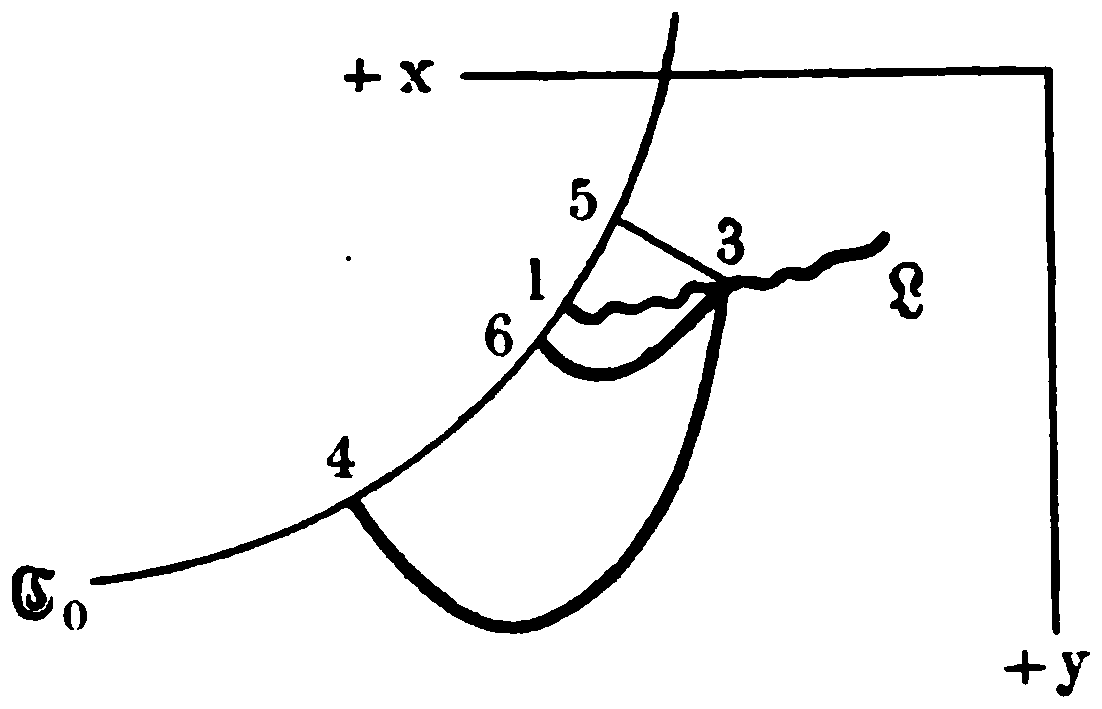
\includegraphics[width=\linewidth,height=35mm,keepaspectratio]{fig_assets/fig18_p0176_src_clean_x8.png}\par\vspace{1mm}
\end{minipage}
\end{center}

% src-pdfpage=0177
% src-break=0177
the curve $\mathfrak{C}_0$, the point 6 is allowed to run from 4 to 5, then it never lies vertically above or below 3 and its normal always passes below the point 3. Therefore an extremal 36 cutting the curve $\mathfrak{C}_0$ perpendicularly and convex downward can always be constructed, for whose length $\mathfrak{R}_{36}$, if $\mathfrak{R}_{35}$ is the rectilinear distance 35, the inequality
\[
\mathfrak{R}_{36}>\mathfrak{R}_{35}
\]
holds, and $\mathfrak{R}_{36}-\mathfrak{R}_{35}$ can be made arbitrarily small. Since plainly
\[
K_{13}\geq \mathfrak{R}_{35},
\]
it follows from inequality (34) that, for at least one position of the point 6,
\[
K_{13}=\mathfrak{R}_{36},
\]
and with this the Weierstrass construction is first carried out for the arc $\Omega_1$. For the rest of the curve $\Omega$, its possibility follows from \S~38 if the variation is made in the manner given there; for the quantity $\Delta$ no longer vanishes here as long as Jacobi's condition for the catenary 02 is fulfilled. The case where the curve $\Omega$ begins with a straight segment normal to $\mathfrak{C}_0$ can be disposed of just as easily as above in Problem IX.

% machine-unit: Kneser_LVR_EN_p0177low_p0192 §§40-42
% appended in continuation package p0177-p0192; §43 excluded.

% src-pdfpage=0177
% src-break=0177-partial-lower
\begin{center}
{\large \S~40.}
\end{center}

The following development holds, whether the extremals of the field have a fixed point 0 in common, or cut a fixed curve $\mathfrak{C}_0$ transversally in the variable point 0.

If one moves along the arc $\mathfrak{C}$ from the point 0 lying on it, let the quantity $\Delta$ vanish for the first time at a point 1 and for such an argument $t=t_1$ that at the place $(t_1,a_0,b_0)$ the functions $\xi,\eta,\omega$ are regular and the quantities $\xi_t,\eta_t$ do not both vanish. Then, in the first of the two cases distinguished above, the point 1 is called conjugate to the point 0; in the second, it is called the extremal focal point of the curve $\mathfrak{C}_0$ for the problem under consideration, and one has the characteristic property
\begin{equation}\tag{35}
\Delta(t_1,a_0,b_0)=0.
\end{equation}
The development attached in \S~36 to equations (10), (11) then gives instructions for constructing a curve 01 along
% src-pdfpage=0178
% src-break=0178
which the \textsc{Weierstrass} construction is possible, while the quantity $\mathfrak{E}$ vanishes everywhere, so that the equations
\begin{equation}\tag{36}
\bar J_{01}=J_{01},\quad \bar K_{01}=K_{01}
\end{equation}
result, and with them the extremum ceases. For this purpose let $t$ first be defined as a function of $a$ and $b$ by the equation
\begin{equation}\tag{37}
\Delta(t,a,b)=0;
\end{equation}
suppose that
\[
\Delta_t(t_1,a_0,b_0)\gtrless 0,
\]
then, with regard to equation (35), one obtains for $t$ an expression
\[
t=t_1+[a-a_0,b-b_0]_1.
\]
We further posit the differential equation
\[
\left|\begin{array}{cc}
\xi_tdt+\xi_a da+\xi_b db&\eta_tdt+\eta_a da+\eta_b db\\[.6ex]
\xi_t&\eta_t
\end{array}\right|=0
\]
or
\begin{equation}\tag{38}
(\xi_t\eta_a-\xi_a\eta_t)\,da+(\xi_t\eta_b-\xi_b\eta_t)\,db=0,
\end{equation}
and substitute for $t$ the expression just obtained; then the factors of $da$ and $db$ are power series in the arguments $a-a_0$, $b-b_0$, which for $a=a_0$, $b=b_0$ do not both vanish, provided we introduce the assumption that the determinants of second order in the matrix
\begin{equation}\tag{39}
\begin{array}{ccc}
\xi_t&\xi_a&\xi_b\\
\eta_t&\eta_a&\eta_b
\end{array}
\end{equation}
do not all vanish for the system of values $t=t_1$, $a=a_0$, $b=b_0$. For if those two factors had the value zero, the same would follow for the third determinant of the matrix, since $\xi_t$ and $\eta_t$ do not both vanish. Thus equation (38), if $a_0$ and $b_0$ are to be corresponding values, gives a relation of one of the forms
\[
b-b_0=[a-a_0]_1,\quad a-a_0=[b-b_0]_1.
\]
If, for example, the first equation holds, and if the obtained values of $b$ and $t$ are substituted in the equations
\begin{equation}\tag{40}
x=\xi(t,a,b),\quad y=\eta(t,a,b),
\end{equation}
then $x$ and $y$ appear in the form of expressions $[a-a_0]_0$, and for $a=a_0$ one has in particular
\[
x=x_1,\quad y=y_1.
\]
Thus equations (40) represent a curve $\mathfrak{C}$ containing the point 1, which in the neighborhood of this point, apart from
% src-pdfpage=0179
% src-break=0179
that point itself, is regular. If the point 1 were a point of return, one would have for it the equations
\[
\xi_tdt+\xi_a da+\xi_b db=0,\quad \eta_tdt+\eta_a da+\eta_b db=0;
\]
since now the equation
\[
\Delta_tdt+\Delta_a da+\Delta_b db=0
\]
holds and one of the quantities $\dfrac{db}{da}$ and $\dfrac{da}{db}$ is different from zero, it would follow that
\begin{equation}\tag{41}
\frac{\partial(\xi,\eta,\Delta)}{\partial(t,a,b)}=0.
\end{equation}
Thus, if this equation does not hold for $t=t_1$, $a=a_0$, $b=b_0$, then the curve $\mathfrak{C}$ has no point of return at the point 1.

It follows now from equation (38), since $\xi_t$ and $\eta_t$ do not vanish simultaneously, that one may set
\begin{equation}\tag{42}
\xi_tdt+\xi_a da+\xi_b db=m\xi_tdt,\quad
\eta_tdt+\eta_a da+\eta_b db=m\eta_tdt;
\end{equation}
the curve $\mathfrak{C}$ is therefore touched at every point by the extremal (40) belonging to the same system of values $(a,b)$, and is the envelope of a certain simply infinite family of these curves.

From equations (42), on the basis of equation (37) and of the assumption introduced concerning the system (39), one obtains
\[
\omega_tdt+\omega_a da+\omega_b db=m\omega_tdt,
\]
or, since evidently one may set
\[
\omega_t=G(\xi,\eta,\xi_t,\eta_t),
\]
\[
\omega_tdt+\omega_a da+\omega_b db=mG(\xi,\eta,\xi_t,\eta_t)dt.
\]
If now $mdt$ is positive, then from this, because of the homogeneity of the function $G$ and equations (42), one may conclude that
\[
\omega_tdt+\omega_a da+\omega_b db
=G(\xi,\eta,\xi_tdt+\xi_a da+\xi_b db,\eta_tdt+\eta_a da+\eta_b db).
\]
The differentials $dt,da,db$ all refer to the progression along the curve $\mathfrak{C}$; if otherwise the increments corresponding to this progression are denoted by $D$, then the last equation and equations (42) may be written
\[
Dx=m\xi_tdt,
\quad Dy=m\eta_tdt,
\quad D\omega=G(\xi,\eta,Dx,Dy).
\]
% src-pdfpage=0180
% src-break=0180
Consequently, if the unprimed integral sign $K$ is referred to the curve $\mathfrak{C}$ and 3 is a point of it (Fig.~19), from the equation
\[
DK_{31}=-G(x,y,Dx,Dy)
\]
one obtains for $mdt>0$ the result
\begin{equation}\tag{43}
D\omega+DK_{31}=D(\bar K_{03}+K_{31})=0,
\end{equation}
where the primed $K$ refers to that extremal 03 which is defined by the system of values $(a,b)$ belonging to the point 3. These extremals therefore furnish, for the curve $\mathfrak{C}$, the \textsc{Weierstrass} construction, and the quantity
\[
\mathfrak{E}(x,y,x',y',Dx,Dy)=\mathfrak{E}(x,y,\xi_t,\eta_t,Dx,Dy)
\]
vanishes therein in the regular manner when $mdt$ is positive.

\begin{center}
\textbf{Fig. 19.}\par\vspace{1mm}
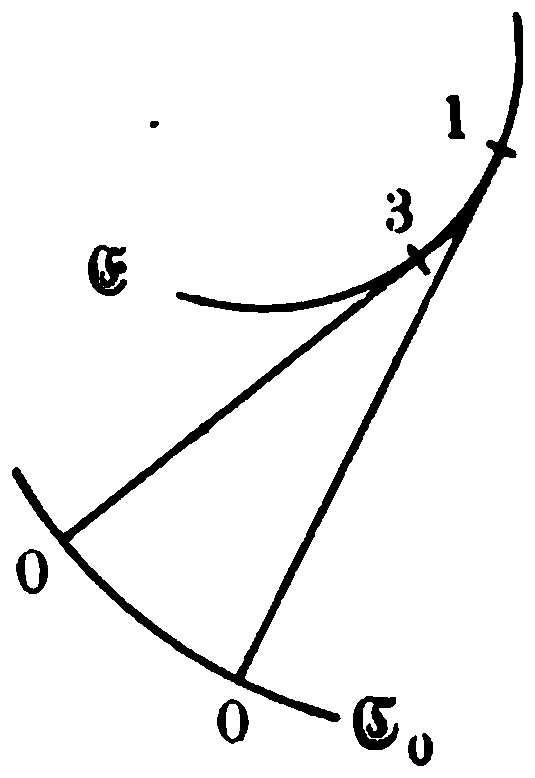
\includegraphics[width=.34\linewidth,height=55mm,keepaspectratio]{fig_assets/fig19_p0180_src_clean_x8.png}
\end{center}

In order to be able to infer equations (36) from this, the sign $D$ must signify the progression on the curve $\mathfrak{C}$ in the direction toward the point 1. This direction may agree with the direction of increasing $t$ on the extremal touching at the point 3, or it may not. The latter case will always occur when the curve $\mathfrak{C}$ has at the point 1 a point of return from which both branches of the curve issue in the direction of the curve $\mathfrak{C}$ traversed with increasing $t$; if the two branches have the opposite direction, or if no point of return is present at all, then in at least one of the two halves into which the curve $\mathfrak{C}$ is divided by this point in the neighborhood of the point 1, the direction of the curve $\mathfrak{C}$ toward the point 1 agrees with the direction of increasing values of $t$ on the extremal 03; this half is denoted by $\mathfrak{C}_1$. The latter direction is defined by the pair of values
\[
x'=\xi_t,
\quad y'=\eta_t;
\]
on the half $\mathfrak{C}_1$, therefore, $Dx$ differs from $\xi_t$ and $Dy$ from $\eta_t$ by a positive factor, so that $mdt$ is positive, and accordingly the indicated quantity $\mathfrak{E}$ vanishes. Such an arc $\mathfrak{C}_1$ is therefore certainly present when equation (41) does not hold and a point of return is thereby excluded.

Let 3 now be any point of the arc $\mathfrak{C}_1$ lying arbitrarily near 1; then the extremal 03 constructed above
% src-pdfpage=0181
% src-break=0181
with the arc 31 of the curve $\mathfrak{C}_1$ forms a connected broken curve with continuously changing tangent, which differs arbitrarily little from the arc 01 belonging to the curve $\mathfrak{C}$, and in such a way that in neighboring points of the two curves the tangents also differ only little. In doing so one has the equation
\[
d(\bar J_{03}+J_{31})=\mathfrak{E}(x,y,x',y',Dx,Dy)=0;
\]
for the expressions for the partial differential quotients of $\bar J_{03}$ and $J_{31}$, which were derived above, remain valid also in the neighborhood of the place $(t_1,a_0,b_0)$, because the indicated integrals are also here regular functions of $t,a,b$. From the equation obtained and the equation (43) characteristic for the \textsc{Weierstrass} construction, there follows
\[
\bar J_{03}+J_{31}=\bar J_{01},
\quad \bar K_{03}+K_{31}=\bar K_{01}.
\]
The arc 01 of the curve $\mathfrak{C}$ therefore no longer furnishes an extremum of the integral $J$ in comparison with all curves which give the same value of the integral $K$; rather, because of the stated properties of the broken curve 031, even the weak extremum already ceases at the point 1.

\noindent\textbf{Example. Problem IX} is to be specialized in the following way. From a given point of one side of an angle, on the convex side, to draw to the other side a line of given length which encloses with the sides an area as large as possible.

Let the second side be the line $y=0$; the area to be extremized differs from the integral $\int yx' dt$ only by the constant triangular area which the perpendicular dropped from the given point to the second side cuts off from the angle. The extremals which cut the line $y=0$ transversally stand perpendicular to it (\S~34) and are circles; hence they can be represented by the equations
\begin{equation}\tag{44}
x=a+b\cos t,
\quad y=b\sin t.
\end{equation}
For the point 0 one always has $t=0$, so that
\[
\bar K_{03}=\omega(t,a,b)=bt.
\]
From this one obtains
\[
\Delta=\begin{vmatrix}
-b\sin t&b\cos t&b\\
1&0&0\\
\cos t&\sin t&t
\end{vmatrix}=b(\sin t-t\cos t);
\]
% src-pdfpage=0182
% src-break=0182
the extremal focal point of the straight line $y=0$ on each circle orthogonal to it is therefore defined by the smallest root of the equation
\[
\tg t=t,
\]
which is denoted by $t_1$ and has approximately the value
\[
t_1=\frac{257\frac{1}{2}}{360}\cdot 2\pi,
\]
that is, corresponds to the angle $257\frac{1}{2}^{\circ}$. Equation (38), which gives the relation defining the curve $\mathfrak{C}$, becomes simply
\[
b\,db+b\cos t_1\,da=0,
\quad db+\cos t_1\,da=0.
\]
Such a relation between $a$ and $b$ singles out from the doubly infinite family of circles (44) a simply infinite one of such circles as touch two fixed straight lines; if $\alpha$ is the concave angle of these lines, then
\[
\sin\frac{\alpha}{2}=-\cos t_1=\cos(t_1-\pi),
\quad \frac{\alpha}{2}=\frac{3\pi}{2}-t_1=12\frac{1}{2}^{\circ}.
\]
On this family the cessation of the extremum can be made evident by elementary means (Fig.~20). Namely, if 1 and 3 are two points lying on the same side of the angle $\alpha$, with 3 nearer to the vertex than 1, and if further $0_0,0$ are the points of intersection of the circles of the family passing through 1 and 3 with the bisector of the angle $\alpha$, and if the arcs $10_0$, 30 have the central angle $t_1$, then the arc $10_0$ and the composite line 130 have equal length; if from 1 the perpendicular 14 is dropped to the bisector of the angle $\alpha$, then the horizontally shaded figure $10_0 41$ and the

\begin{center}
\textbf{Fig. 20.}\par\vspace{1mm}
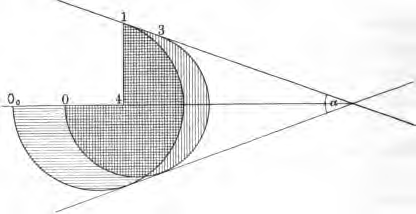
\includegraphics[width=.70\linewidth,height=40mm,keepaspectratio]{fig_assets/fig20_p0182_src_clean_x8.png}
\end{center}

% src-pdfpage=0183
% src-break=0183
vertically shaded figure 13041 have equal area, so that the arc $10_0$ certainly does not furnish an extremum of the area for prescribed arc length. The arc $\mathfrak{C}_1$ is the straight segment 13.

\begin{center}
{\large \S~41.}
\end{center}

Let the point 0 be chosen on the extremal $\mathfrak{C}$ so that $\xi_t$ does not vanish; then the differential equation of the extremals can be written in the form
\[
f_y+\lambda g_y-\frac{d(f_p+\lambda g_p)}{dx}=0,
\]
and gives for $\dfrac{dp}{dx}$ an expression regular with respect to $x,y,p$ when the inequality
\begin{equation}\tag{45}
f_{pp}+\lambda g_{pp}\gtrless 0
\end{equation}
holds. Under this assumption, the general theorem of \S~27 then teaches that the differential equation possesses an integral of the form
\begin{equation}\tag{46}
y=\Phi(x,a,b,\lambda),
\end{equation}
which for $a=a_0$, $b=b_0$, $\lambda=\lambda_0$ leads to the curve $\mathfrak{C}$, and is regular at the place $(x_{00},a_0,b_0,\lambda_0)$, if $x_{00}$ denotes the abscissa of the point 0. If, in particular, for $a$ and $b$ one takes the values of $y$ and $p$ for $x=x_{00}$, then
\[
\Phi(x,a,b,\lambda)=a+b(x-x_{00})+[x-x_{00}]_2
\]
and for $x=x_{00}$
\begin{equation}\tag{47}
\Phi_b=0,
\quad \Phi_{bx}=1.
\end{equation}
We now seek to single out from the threefold manifold of extremals given by equation (46) a twofold one which cuts transversally a regular curve $\mathfrak{C}_0$ issuing from the point 0, whose equation is
\[
y_0=\gamma(x_0).
\]
This happens if the following equations are fulfilled:
\begin{equation}\tag{48}
\begin{aligned}
M&=\Phi(x_0,a,b,\lambda)-\gamma(x_0)=0,\\
N&=f+\lambda g-p(f_p+\lambda g_p)+(f_p+\lambda g_p)\gamma'(x)\big|_{x=x_0}=0;
\end{aligned}
\end{equation}
% src-pdfpage=0184
% src-break=0184
in the second equation the values $\Phi$ and $\Phi_x$ are to be substituted for $y$ and $p$. The left sides of these equations are regular at the place $x_0=x_{00}$, $a=a_0$, $b=b_0$, $\lambda=\lambda_0$; it is easy to see when from them two of the quantities $x,a,b,\lambda$ can be expressed as functions of the remaining ones. Namely, forming
\[
\frac{\partial(M,N)}{\partial(x_0,b)}=
\left|\begin{array}{cc}
\Phi_x-\gamma'(x)&\Phi_b\\[.6ex]
\dfrac{\partial N}{\partial x}+\Phi_x\dfrac{\partial N}{\partial y}+\Phi_{xx}\dfrac{\partial N}{\partial p}&
\dfrac{\partial N}{\partial y}\Phi_b+\dfrac{\partial N}{\partial p}\Phi_{bx}
\end{array}\right|_{x=x_0}
\]
and observing that evidently
\[
\frac{\partial N}{\partial p}=[\gamma'(x)-\Phi_x](f_{pp}+\lambda g_{pp})\big|_{x=x_0},
\]
one obtains, by equations (47), for $x=x_{00}$
\[
\frac{\partial(M,N)}{\partial(x_0,b)}=-[\gamma'(x)-\Phi_x]^2(f_{pp}+\lambda g_{pp})\big|_{x=x_{00}}
\]
and this expression is different from zero at the place $(x_{00},a_0,b_0,\lambda_0)$ if
\[
\Phi_x(x_{00},a_0,b_0,\lambda_0)-\gamma'(x_{00})\gtrless 0,
\]
that is, if the curves $\mathfrak{C}$ and $\mathfrak{C}_0$ do not touch one another. Then equations (48) give for $b-b_0$ and $x_0-x_{00}$ expressions of the form
\[
[a-a_0,\lambda-\lambda_0]_1;
\]
if in $\Phi$ the former is substituted for $b-b_0$, one obtains an expression
\begin{equation}\tag{49}
y=\varphi(x,a,\lambda),
\end{equation}
which is regular at the place $(x_{00},a_0,\lambda_0)$ and defines the doubly infinitely many extremals cutting the curve $\mathfrak{C}_0$ transversally. If the curve $\mathfrak{C}_0$ contracts to the point 0, the same result follows, that is, an equation of the extremals passing through this point, simply by solving the equation
\begin{equation}\tag{50}
\Phi(x_{00},a,b,\lambda)-y_{00}=0
\end{equation}
for $b$.

In each of these cases a relation between $a,b,\lambda$ is established by an equation
\begin{equation}\tag{51}
\Omega(a,b,\lambda)=0
\end{equation}
for which
% src-pdfpage=0185
% src-break=0185
\begin{equation}\tag{52}
\Omega_b(a_0,b_0,\lambda_0)\gtrless 0
\end{equation}
and the left side is regular in the neighborhood of the place $(a_0,b_0,\lambda_0)$. In doing so one evidently obtains
\[
\Omega_a+\Omega_b\frac{\partial b}{\partial a}=0,
\quad
\Omega_\lambda+\Omega_b\frac{\partial b}{\partial \lambda}=0,
\]
\[
\varphi_a(x,a,\lambda)=\Phi_a+\Phi_b\frac{\partial b}{\partial a},
\quad
\varphi_\lambda(x,a,\lambda)=\Phi_\lambda+\Phi_b\frac{\partial b}{\partial\lambda},
\]
and analogous equations hold for every quantity which first appears as a function of $a,b,\lambda$, and then passes into one of $a$ and $\lambda$ alone.

If, for example, one sets
\[
\Theta(x,a,b,\lambda)=\int_{x_0}^{x}g(x,\Phi,\Phi_x)\,dx
\]
and if, under assumption (51), this quantity passes into $\omega(x,a,\lambda)$, then for the extremals (49), since $t=x$ may be set, it has the same meaning as the earlier quantity $\omega(t,a,b)$, and one obtains for $\Delta$, by replacing $b$ by $\lambda$, the following expression:
\[
\begin{aligned}
\Delta&=\frac{\partial(\xi,\eta,\omega)}{\partial(x,a,\lambda)}
=\frac{\partial(\varphi,\omega)}{\partial(a,\lambda)} \\
&=\begin{vmatrix}
\Phi_a+\Phi_b\dfrac{\partial b}{\partial a}&\Phi_\lambda+\Phi_b\dfrac{\partial b}{\partial\lambda}\\[1.0ex]
\Theta_a+\Theta_b\dfrac{\partial b}{\partial a}&\Theta_\lambda+\Theta_b\dfrac{\partial b}{\partial\lambda}
\end{vmatrix}\\
&=\frac{1}{\Omega_b}\begin{vmatrix}
\Phi_a&\Phi_b&\Phi_\lambda\\
\Omega_a&\Omega_b&\Omega_\lambda\\
\Theta_a&\Theta_b&\Theta_\lambda
\end{vmatrix}=\frac{D}{\Omega_b}.
\end{aligned}
\]
If it is possible to prove that this determinant does not vanish identically, then it is shown that the extremals $y=\varphi(x,a,\lambda)$ form, at least in the neighborhood of the point 0, a field in the sense of \S~39.

In order to investigate the determinant last obtained, we proceed from the fact that $x_0$ is defined as a regular function of $a,b,\lambda$; one therefore has the equation
\[
\Theta_a=-g\frac{\partial x_0}{\partial a}\bigg|^0+\int_{x_0}^{x}\frac{\partial g}{\partial a}\,dx
=-g\frac{\partial x_0}{\partial a}\bigg|^0+g_p\Phi_a\bigg|_{x_0}^{x}+\int_{x_0}^{x}\left(g_y-\frac{dg_p}{dx}\right)\Phi_a\,dx
\]
% src-pdfpage=0186
% src-break=0186
together with similar equations in which $a$ is replaced by $b$ or $\lambda$. Hence it follows that
\[
D=\frac{\partial(\Phi,\Omega,\Theta)}{\partial(a,b,\lambda)}
\]
\[
=\begin{vmatrix}
\Phi_a&\Phi_b&\Phi_\lambda\\[.6ex]
\Omega_a&\Omega_b&\Omega_\lambda\\[.6ex]
A+\displaystyle\int_{x_0}^{x}\left(g_y-\frac{dg_p}{dx}\right)\Phi_a\,dx&B+\displaystyle\int_{x_0}^{x}\left(g_y-\frac{dg_p}{dx}\right)\Phi_b\,dx&C+\displaystyle\int_{x_0}^{x}\left(g_y-\frac{dg_p}{dx}\right)\Phi_\lambda\,dx
\end{vmatrix},
\]
where the quantities $A,B,C$ are independent of $x$; for the terms preceding the integral sign in the expressions $\Theta_a,\Theta_b,\Theta_\lambda$ which depend on $x$ drop out if the first row of the determinant is multiplied by $g_p$ and subtracted from the last. If now this expression $D$ vanished identically, then, first, the determinants of second order of the matrix
\begin{equation}\tag{53}
\left\|\begin{array}{ccc}
\Omega_a&\Omega_b&\Omega_\lambda\\[.8ex]
A+\displaystyle\int_{x_0}^{x}\cdots&B+\displaystyle\int_{x_0}^{x}\cdots&C+\displaystyle\int_{x_0}^{x}\cdots
\end{array}\right\|
\end{equation}
could vanish identically at the same time. Their differential quotients with respect to $x$ are the determinants of the matrix
\[
\left\|\begin{array}{ccc}
\Omega_a&\Omega_b&\Omega_\lambda\\[.8ex]
\left(g_y-\dfrac{dg_p}{dx}\right)\Phi_a&
\left(g_y-\dfrac{dg_p}{dx}\right)\Phi_b&
\left(g_y-\dfrac{dg_p}{dx}\right)\Phi_\lambda
\end{array}\right\|;
\]
since now on the curve $\mathfrak{C}$ as extremal in the problem of the relative extremum the quantity
\[
R=g_y-\frac{dg_p}{dx}
\]
does not vanish, the determinants of the matrix
\[
\left\|\begin{array}{ccc}
\Omega_a&\Omega_b&\Omega_\lambda\\
\Phi_a&\Phi_b&\Phi_\lambda
\end{array}\right\|
\]
would also vanish, for example
\begin{equation}\tag{54}
\Omega_a\Phi_b-\Omega_b\Phi_a=0,
\quad
\Omega_\lambda\Phi_b-\Omega_b\Phi_\lambda=0.
\end{equation}
The first of these equations is however plainly impossible, since for $x=x_{00}$, $a=a_0$, $b=b_0$, $\lambda=\lambda_0$
% src-pdfpage=0187
% src-break=0187
\begin{equation}\tag{55}
\Phi_a=1,
\quad \Phi_b=0,
\quad \Omega_b\gtrless 0;
\end{equation}
the second is impossible because $\Phi_b$ begins with the first, $\Phi_\lambda$ with a higher power of $x-x_{00}$; the quantity $\Phi_\lambda$ cannot vanish identically, because otherwise the expression $\Phi$ would be independent of $\lambda$, and therefore would also satisfy the equation
\[
f_y-\frac{df_p}{dx}=0,
\]
whose left side, like $R$, is different from zero for the curve $\mathfrak{C}$.

In particular it follows from this consideration that none of the determinants
\begin{equation}\tag{56}
\left|\begin{array}{cc}
\Omega_a&\Omega_b\\[.8ex]
A+\displaystyle\int_{x_0}^{x}R\Phi_a\,dx&B+\displaystyle\int_{x_0}^{x}R\Phi_b\,dx
\end{array}\right|,
\quad
\left|\begin{array}{cc}
\Omega_\lambda&\Omega_b\\[.8ex]
C+\displaystyle\int_{x_0}^{x}R\Phi_\lambda\,dx&B+\displaystyle\int_{x_0}^{x}R\Phi_b\,dx
\end{array}\right|
\end{equation}
vanishes identically, since their derivatives are the left sides of equations (54), multiplied by the non-vanishing quantity $R$. But by a general theorem of determinant theory, in a vanishing determinant the adjoints of two parallel rows are proportional; if this theorem is applied to the first and third rows of the determinant $D$, then it follows that the last two determinants are proportional to the left sides of equations (54). Since now neither one of these four quantities nor the quantity $R$ vanishes identically, it follows that the logarithmic derivatives of the quantities (56) with respect to $x$ are equal, and that the quantities themselves therefore stand in the relation
\[
\left|\begin{array}{cc}
\Omega_a&\Omega_b\\[.8ex]
A+\displaystyle\int_{x_0}^{x}R\Phi_a\,dx&B+\displaystyle\int_{x_0}^{x}R\Phi_b\,dx
\end{array}\right|
=M
\left|\begin{array}{cc}
\Omega_\lambda&\Omega_b\\[.8ex]
C+\displaystyle\int_{x_0}^{x}R\Phi_\lambda\,dx&B+\displaystyle\int_{x_0}^{x}R\Phi_b\,dx
\end{array}\right|
\]
% src-pdfpage=0188
% src-break=0188
if by $M$ an $x$-independent, finite, non-zero quantity is denoted. From this follows by differentiation, with regard to the non-vanishing value of the quantity $R$,
\[
\Omega_a\Phi_b-\Omega_b\Phi_a=M(\Omega_\lambda\Phi_b-\Omega_b\Phi_\lambda).
\]
Putting here $x=x_{00}$, the left side reduces to $-\Omega_b$, the right side to zero, since the relations (55) hold. The assumption that $D$ vanishes identically therefore always leads to a contradiction.

On the basis of the relation between $D$ and $\Delta$, the following is hereby proved. If to the earlier assumptions concerning the extremal $\mathfrak{C}$ we add the inequality (45), then the arc beginning at the point 0 can always be surrounded with a field whose extremals either all pass through the point 0, or cut transversally a given regular curve $\mathfrak{C}_0$, not touched by the curve $\mathfrak{C}$ and cut transversally by it at the point 0. Thus for a sufficiently small extremal arc the \textsc{Jacobi} condition of the extremum is fulfilled, whether one or both endpoints of the required curve are held fixed.

\begin{center}
{\large \S~42.}
\end{center}

If the point 0 is fixed and the equation $\Omega=0$ is accordingly replaced by the special relation (50), then one has
\[
\Omega_a=\Phi_a(x_0,a,b,\lambda),
\]
\[
\Omega_b=\Phi_b(x_0,a,b,\lambda),
\quad
\Omega_\lambda=\Phi_\lambda(x_0,a,b,\lambda)
\]
and therefore obtains
\[
D=\frac{\partial\left\{\Phi(x,a,b,\lambda),\ \Phi(x_0,a,b,\lambda),\ \displaystyle\int_{x_0}^{x}g[x,\Phi(x,a,b,\lambda),\Phi_x(x,a,b,\lambda)]\,dx\right\}}{\partial(a,b,\lambda)}.
\]
Since this expression has the value
\[
\Delta\Phi_b(x_0,a,b,\lambda),
\]
the quantity
\[
\Delta(x_0,x)=D\big|_{a=a_0,\,b=b_0,\,\lambda=\lambda_0}
\]
% src-pdfpage=0189
% src-break=0189
vanishes when the points 0 and $(x,y)$ are conjugate. Thus \textsc{Mayer}'s criterion of conjugate points has been derived. The analogous formula of \textsc{Weierstrass} is obtained under the assumption that the extremals are represented in the form
\begin{equation}\tag{57}
x=X(t,a,b,\lambda),
\quad y=Y(t,a,b,\lambda).
\end{equation}
Then one has the identity
\[
Y=\Phi(X,a,b,\lambda)
\]
and the relations following from it
\[
\begin{gathered}
Y_t=\Phi_x(X,a,b,\lambda)X_t,
\quad Y_a=\Phi_xX_a+\Phi_a,
\quad Y_b=\Phi_xX_b+\Phi_b,\\
Y_\lambda=\Phi_xX_\lambda+\Phi_\lambda;
\end{gathered}
\]
\[
X_t\Phi_a=X_tY_a-X_aY_t=\theta_1(t),
\]
\[
X_t\Phi_b=X_tY_b-X_bY_t=\theta_2(t),
\quad
X_t\Phi_\lambda=X_tY_\lambda-X_\lambda Y_t=\theta_3(t).
\]
If therefore the point 0 belongs to the argument $t=t_0$, then
\[
D X_t(t,a,b,\lambda)X_t(t_0,a,b,\lambda)=
\begin{vmatrix}
\theta_1(t)&\theta_2(t)&\theta_3(t)\\
\theta_1(t_0)&\theta_2(t_0)&\theta_3(t_0)\\[.6ex]
\dfrac{\partial K}{\partial a}&\dfrac{\partial K}{\partial b}&\dfrac{\partial K}{\partial\lambda}
\end{vmatrix},
\]
where it is set that
\[
K=\int_{x_0}^{x}g\,dx=\int_{t_0}^{t}G(X,Y,X_t,Y_t)\,dt.
\]
Now, since $x_0$ does not depend on $a,b,\lambda$, one has the equation
\[
\frac{\partial K}{\partial a}=\Phi_a g_p\bigg|_{x_0}^{x}+\int_{x_0}^{x}\Phi_a\left(g_y-\frac{dg_p}{dx}\right)dx
\]
together with similar formulas in which $a$ is replaced by $b$ and $\lambda$; if therefore in the determinant $D$ the first rows are added to the last after multiplication by suitable factors, then the latter becomes
\[
\int_{x_0}^{x}\Phi_a\left(g_y-\frac{dg_p}{dx}\right)dx,
\quad
\int_{x_0}^{x}\Phi_b\left(g_y-\frac{dg_p}{dx}\right)dx,
\quad
\int_{x_0}^{x}\Phi_\lambda\left(g_y-\frac{dg_p}{dx}\right)dx.
\]
Furthermore one has, by \S~5, if
\[
G(x,y,x',y')=x'g\left(x,y,\frac{y'}{x'}\right)
\]
is introduced,
% src-pdfpage=0190
% src-break=0190
\[
x'\left(g_y-\frac{dg_p}{dx}\right)=G_y-G'_{y'}=-\frac{x'}{y'}(G_x-G'_{x'});
\]
from this follows
\[
\Phi_a\left(g_y-\frac{dg_p}{dx}\right)dx=\biggl(Y_a-X_a\frac{Y_t}{X_t}\biggr)(G_y-G'_{y'})dt
\]
\[
=[X_a(G_x-G'_{x'})+Y_a(G_y-G'_{y'})]dt.
\]
If therefore one sets
\[
\Theta_1(t_0,t)=\int_{t_0}^{t}dt\,[X_a(G_x-G'_{x'})+Y_a(G_y-G'_{y'})]
\]
and lets $\Theta_2$ and $\Theta_3$ arise from this by replacing $a$ by $b$ and $\lambda$, then one obtains the \textsc{Weierstrass} determinant
\[
D X_t(t,a,b,\lambda)X_t(t_0,a,b,\lambda)=
\begin{vmatrix}
\theta_1(t)&\theta_2(t)&\theta_3(t)\\
\theta_1(t_0)&\theta_2(t_0)&\theta_3(t_0)\\
\Theta_1(t_0,t)&\Theta_2(t_0,t)&\Theta_3(t_0,t)
\end{vmatrix}=D(t_0,t).
\]
Here it is to be observed that $D$ is defined only under the assumption that in the interval $t_0\ldots t$ the curve $\mathfrak{C}$ everywhere defines $y$ as a regular function of $x$. The right side, by contrast, has meaning for every arc $\mathfrak{C}$ along which $x$ and $y$ are regular functions of $t$ and the quantity $H_1(x,y,x',y')$ does not vanish; for such an arc can by \S~27 always be embedded in a family of curves such as is represented by equations (57).

If $D(t_0,t)$ does not vanish identically, at least one of the quantities $\theta_1(t_0),\theta_2(t_0),\theta_3(t_0)$ is different from zero. Let this be, for example, the last; then $t_0$ and $\lambda$ can be calculated from the equations
\[
x_0=X(t_0,a,b,\lambda),
\quad y_0=Y(t_0,a,b,\lambda)
\]
as regular functions of $a$ and $b$; substituting them, one obtains
\[
X=\xi(t,a,b),
\quad Y=\eta(t,a,b).
\]
Then the following equations hold:
\[
X_t\frac{\partial t_0}{\partial a}+X_\lambda\frac{\partial\lambda}{\partial a}+X_a\bigg|^{t_0}=Y_t\frac{\partial t_0}{\partial a}+Y_\lambda\frac{\partial\lambda}{\partial a}+Y_a\bigg|^{t_0}=0,
\]
\[
X_t\frac{\partial t_0}{\partial b}+X_\lambda\frac{\partial\lambda}{\partial b}+X_b\bigg|^{t_0}=Y_t\frac{\partial t_0}{\partial b}+Y_\lambda\frac{\partial\lambda}{\partial b}+Y_b\bigg|^{t_0}=0,
\]
% src-pdfpage=0191
% src-break=0191
\[
\xi_t=X_t,
\quad \eta_t=Y_t,
\quad X_a+X_\lambda\frac{\partial\lambda}{\partial a}=\xi_a,
\quad Y_a+Y_\lambda\frac{\partial\lambda}{\partial a}=\eta_a,
\]
\[
X_b+X_\lambda\frac{\partial\lambda}{\partial b}=\xi_b,
\quad Y_b+Y_\lambda\frac{\partial\lambda}{\partial b}=\eta_b.
\]
From the first four equations it follows easily that
\[
\theta_1(t_0)+\theta_3(t_0)\frac{\partial\lambda}{\partial a}=\theta_2(t_0)+\theta_3(t_0)\frac{\partial\lambda}{\partial b}=0,
\]
from the last four that
\[
\theta_1(t)+\theta_3(t)\frac{\partial\lambda}{\partial a}=\xi_t\eta_a-\xi_a\eta_t,
\quad
\theta_2(t)+\theta_3(t)\frac{\partial\lambda}{\partial b}=\xi_t\eta_b-\xi_b\eta_t,
\]
and the definition of the quantities $\Theta$ gives
\[
\Theta_1(t_0,t)+\frac{\partial\lambda}{\partial a}\Theta_3(t_0,t)=
\int_{t_0}^{t}dt\{(G_x-G'_{x'})\xi_a+(G_y-G'_{y'})\eta_a\}=A,
\]
\[
\Theta_2(t_0,t)+\frac{\partial\lambda}{\partial b}\Theta_3(t_0,t)=
\int_{t_0}^{t}dt\{(G_x-G'_{x'})\xi_b+(G_y-G'_{y'})\eta_b\}=B.
\]
If therefore in the determinant $D(t_0,t)$ the third vertical column, multiplied by $\partial\lambda:\partial a$ and $\partial\lambda:\partial b$, is added to the first and second, one obtains
\[
D(t_0,t)=-\theta_3(t_0)\begin{vmatrix}
\xi_t\eta_a-\xi_a\eta_t&\xi_t\eta_b-\xi_b\eta_t\\
A&B
\end{vmatrix}.
\]
Since now, by \S~35,
\[
\omega_a=G_{x'}\xi_a+G_{y'}\eta_a+A,
\quad
\omega_b=G_{x'}\xi_b+G_{y'}\eta_b+B,
\]
\[
\omega_t=G=\xi_tG_{x'}+\eta_tG_{y'},
\]
it follows finally that
\[
D(t_0,t)=-\theta_3(t_0)\frac{\partial(\xi,\eta,\omega)}{\partial(t,a,b)}=-\theta_3(t_0)\Delta.
\]
Under the introduced assumption, therefore, $\Delta$ and $D(t_0,t)$ vanish only simultaneously, and the equation
\[
D(t_0,t)=0
\]
is, as soon as its left side does not vanish identically, a sufficient and necessary condition that conjugate points belong to the arguments $t_0$ and $t$. If, therefore, the quantity $D(t_0,t)$, apart from the point 0 itself, is different from zero everywhere on an arc 02, then an extremum
% src-pdfpage=0192
% src-break=0192
of the required kind results for every arc 12 whose initial point is arbitrarily little different from 0.

From this it follows, on the basis of the consideration carried out at the end of \S~31, that for the arc 12 with fixed endpoints the \textsc{Jacobi} condition of the extremum can in general also be formulated as follows: the equation
\[
D(t_1,t)=0
\]
has on the segment 12 no root other than $t=t_1$; for that consideration can be applied without any alteration to the quantity now denoted by $D(t_0,t)$ as soon as the inequality
\[
\frac{\partial D(t_0,t)}{\partial t}\bigg|_{t=t_0}\gtrless 0
\]
holds. Even when the quantities
\[
d_\alpha(t_0)=\frac{\partial^\alpha D(t_0,t)}{\partial t^\alpha}\bigg|_{t=t_0}
\]
vanish identically for $\alpha=1,2,\ldots n$, but $d_{n+1}(t_1)$ is different from zero, the argument of \S~31 needs to be modified only insofar as the quantity $d_{n+1}(t_0)$ takes the place of $f_1(t_0)$. Only when $d_{n+1}(t_0)$ does not vanish identically, but $d_{n+1}(t_1)$ has the value zero, does it become doubtful whether the cited consideration can be applied.


% machine-manifest-begin
% {"work": "Kneser_LVR", "language": "en", "branch": "canonical_complete_volume", "source_pdf_pages": "author-clean cumulative p0011-p0335; sections 1-69, Literature, printed errata, and unnumbered addendum complete; p0336 rear board excluded by evidence ledger", "visible_text_policy": "authorial text only; no vendor marks, source captions, running heads, page numbers, signatures, or preservation/library notes", "math_policy": "all displayed and inline mathematical symbols retained as TeX; provenance appears only in comments and external ledgers", "figure_policy": "figures 1--24 retained as HQ source-derived whitened original crops only; no visible drawn/TikZ layer", "description": "complete aligned faithful English translation", "completion_boundary": "source PDF335; PDF336 rear board excluded", "errata_policy": "printed errata transcribed as printed; body corrections not silently applied"}
% machine-manifest-end

% machine-unit: Kneser_LVR_EN_p0193_p0206 §§43-45
% src-pdfpage=0193
\begin{center}
{\large Fifth Section.}\\[1.1ex]
{\Large\bfseries Discontinuous Solutions.}\\[2ex]
\rule{32mm}{0.4pt}\\[2ex]
{\large \S~43.}
\end{center}

The developments of the preceding sections do not always give a solution of the original problem of the extremum: to draw, between two given points, a curve which supplies an absolute or relative extremum of the integral $J$. It was only shown that the sought curve, if it is to have certain continuity properties, can be nothing other than a regular piece of an extremal; conditions of the extremum were then derived under the assumption that the two given endpoints of the sought curve were already connected by an arc of an extremal free from singularities. If this assumption is not fulfilled, which happens even in simple problems, then the sought extremum cannot be supplied by a curve with the assumed continuity properties; and one is therefore led to the question whether a curve affected by singularities, for example corners, may solve the proposed problem. If one succeeds in answering this question by admitting definite classes of singularities, then one still has no infallible method for determining the desired extremum; but the circle of cases in which the problem can be solved is enlarged.

In particular, we ask when the integral
\[
J=\int Fdt
\]
is made an absolute extremum by a curve which consists of a finite number of pieces meeting at corners,
% src-pdfpage=0194
of which each possesses the properties previously required for the whole curve; that is, along each piece $x$ and $y$ are continuous functions of a parameter $t$, furnished with continuous first and second derivatives. For each one of these pieces separately the considerations of the second section remain valid, since one may leave the corners unchanged and restrict the variation to the interior of the pieces; each of them must therefore be an arc of an extremal.

\begin{center}
{\small Fig. 21.}\par\vspace{1mm}
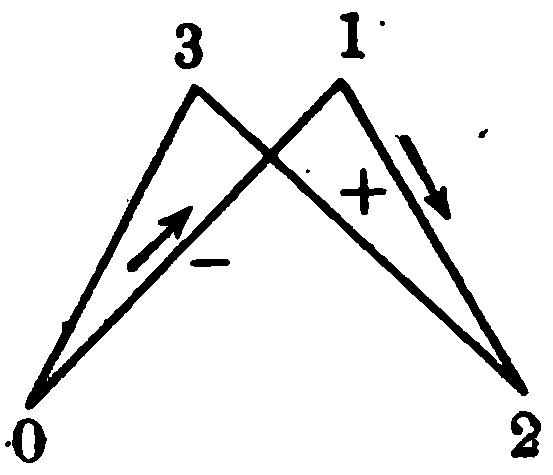
\includegraphics[width=.34\linewidth,height=33mm,keepaspectratio]{fig_assets/fig21_p0194_src_clean_x8.png}
\end{center}

On the arcs meeting at the corner 1 let the points 0 and 2 be chosen so near the corner that the arcs 01 and 12 contain no pair of conjugate points (Fig.~21). Then the points 0 and 2 may be joined with every point 3 sufficiently little removed from 1 by extremals 03 and 32, and these may, by \S~2, be regarded as a variation of the arcs 01 and 12. The broken line 012, as part of the sought curve, may therefore, since the variation formulae of \S~2 remain valid for each of the parts 01 and 02, be replaced by 032. Put
\[
\delta x_1=x_3-x_1,\quad \delta y_1=y_3-y_1
\]
and provide the symbol of any quantity with the sign $-$ or $+$ according as it is to be formed for the arc 01 in the direction beyond 1, or for the arc 12 in the direction toward 2. Then one has the formulae
\[
\Delta \overline{J}_{01}=F_{x'}^-\delta x+F_{y'}^-\delta y\big|^1+[\delta x_1,\delta y_1]_2,
\]
\[
\Delta \overline{J}_{12}=-F_{x'}^+\delta x-F_{y'}^+\delta y\big|^1+[\delta x_1,\delta y_1]_2,
\]
\[
F_{x'}^- =F_{x'}(x,y,x'_{-},y'_{-}),\quad
F_{x'}^+=F_{x'}(x,y,x'_{+},y'_{+}),\ldots,
\]
and hence, on adding,
\[
\Delta\overline{J}_{012}=(F_{x'}^- -F_{x'}^+)\delta x+(F_{y'}^- -F_{y'}^+)\delta y\big|^1+[\delta x_1,\delta y_1]_2.
\]
This quantity must have a constant sign if the curve to which the polygonal line 012 belongs is to give an extremum of the integral $J$. If, therefore, the corner point 3 is freely disposable near the position 1, so that the quantities $\delta x_1$, $\delta y_1$ are independent of one another, the coefficients of the linear terms must vanish (\S~7), and one obtains \textsc{Erdmann}'s theorem
% src-pdfpage=0195
\begin{equation}\tag{1}
F_{x'}^- =F_{x'}^+,
\quad F_{y'}^- =F_{y'}^+.
\end{equation}
If, on the other hand, the corner point is from the outset bound to the curve
\begin{equation}\tag{2}
h(x_1,y_1)=0,
\end{equation}
so that the equation
\[
0=h_x(x_1,y_1)\delta x_1+h_y(x_1,y_1)\delta y_1+[\delta x_1,\delta y_1]_2
\]
holds, then, by \S~7, $\Delta\overline{J}_{012}$ can have an invariable sign only if
\[
\begin{vmatrix}
F_{x'}^- -F_{x'}^+&F_{y'}^- -F_{y'}^+\\
h_x(x_1,y_1)&h_y(x_1,y_1)
\end{vmatrix}=0,
\]
that is, if for an infinitely small displacement of the point 1 on the curve (2) the equation
\begin{equation}\tag{3}
F_{x'}^-\delta x_1+F_{y'}^-\delta y_1=F_{x'}^+\delta x_1+F_{y'}^+\delta y_1
\end{equation}
holds.

Denote the segment 13 by $\delta s$, and assume that on each of the extremals 01 and 12 the parameter $t$ denotes the arc which always increases in the direction from 0 through 1 toward 2. Then three angles $\sigma$, $\theta_+$, $\theta_-$ may be introduced, satisfying
\[
\delta x_1=\delta s\cos\sigma,\quad \delta y_1=\delta s\sin\sigma,
\]
\[
x'_{-}=\cos\theta_{-},\quad y'_{-}=\sin\theta_{-},\quad
x'_{+}=\cos\theta_{+},\quad y'_{+}=\sin\theta_{+}.
\]
Define further the quantities $u$, $v$ by the equations
\begin{equation}\tag{4}
\delta x_1=x'_{+}u+x'_{-}v,
\quad \delta y_1=y'_{+}u+y'_{-}v;
\end{equation}
then one readily obtains
\[
u=\frac{\delta s\sin(\sigma-\theta_{-})}{\sin(\theta_{+}-\theta_{-})},
\quad
v=\frac{\delta s\sin(\sigma-\theta_{+})}{\sin(\theta_{-}-\theta_{+})},
\]
and these quantities are proportional to the perpendiculars which can be dropped from the point 3 to the extremals 01 and 12. At the same time equations (4) give
\[
(F_{x'}^- -F_{x'}^+)\delta x_1+(F_{y'}^- -F_{y'}^+)\delta y_1
\]
\[
=u(x'_{+}F_{x'}^-+y'_{+}F_{y'}^- -F^+)-v(x'_{-}F_{x'}^+ + y'_{-}F_{y'}^+ -F^-)
\]
\[
=u\mathfrak{E}(x_1,y_1,x'_{-},y'_{-},x'_{+},y'_{+})
-v\mathfrak{E}(x_1,y_1,x'_{+},y'_{+},x'_{-},y'_{-}),
\]
and, according to the preceding, this expression must vanish for every permitted displacement of the corner point.
% src-pdfpage=0196

\textbf{First example.} The principle of least action in the \textsc{Euler-Jacobi} form for the central motion of a free point in the plane. Let the repulsion be, for example, proportional to the distance; if one sets
\[
r=\sqrt{x^2+y^2},
\]
then the potential is $cr$, and the principle in question asserts that the trajectories make the integral
\[
\int \sqrt{cr+h}\,\sqrt{dx^2+dy^2}
\]
a minimum, where $h$ denotes the constant of the living force. If one assumes in particular $h=0$, then among the trajectories so defined there are the radii issuing from the force centre, along which the moving point can approach the centre asymptotically; and one has to put
\[
F=\sqrt{x^2+y^2}\,\sqrt{x'^2+y'^2}.
\]
Equations (1), when $r$ is different from zero, give the result
\[
\frac{x'_{-}}{\sqrt{x_{-}'{}^2+y_{-}'{}^2}}
=
\frac{x'_{+}}{\sqrt{x_{+}'{}^2+y_{+}'{}^2}},
\quad
\frac{y'_{-}}{\sqrt{x_{-}'{}^2+y_{-}'{}^2}}
=
\frac{y'_{+}}{\sqrt{x_{+}'{}^2+y_{+}'{}^2}},
\]
that is, the directions $+$ and $-$ coincide. A corner can therefore occur only at the force centre ($r=0$). For any two radii issuing from it equations (1) are satisfied. Since, under the assumption $h=0$, the radii are the only trajectories which pass through the force centre, a broken line can give an extremum only if it consists of two straight pieces meeting at the centre.

Similar considerations can be made when the force is proportional to an arbitrary power of the distance; one then has to make the integral
\[
\int (x^2+y^2)^n\sqrt{dx^2+dy^2}
\]
a minimum.

\textbf{Second example.} Problem VII (\S~11). The shortest line on the surface whose line element is given by the formula
\[
ds^2=Edx^2+2Fdxdy+Gdy^2
\]
% src-pdfpage=0197
can nowhere have a freely disposable corner so long as $EG-F^2$ is different from zero. For equations (1) would require
\[
E\left(\frac{dx}{ds}\right)_{-}+F\left(\frac{dy}{ds}\right)_{-}
=E\left(\frac{dx}{ds}\right)_{+}+F\left(\frac{dy}{ds}\right)_{+},
\]
\[
F\left(\frac{dx}{ds}\right)_{-}+G\left(\frac{dy}{ds}\right)_{-}
=F\left(\frac{dx}{ds}\right)_{+}+G\left(\frac{dy}{ds}\right)_{+},
\]
from which, under the stated assumption, it would follow that
\[
\left(\frac{dx}{ds}\right)_{-}-\left(\frac{dx}{ds}\right)_{+}
=
\left(\frac{dy}{ds}\right)_{-}-\left(\frac{dy}{ds}\right)_{+}=0.
\]
A corner can, however, occur if it is required to join the points 0 and 2 by the shortest line which has in common with a given curve a point 1 which is not prescribed. Let $D$ denote the increment in proceeding along this curve, and let $Ds$ be its arc element; then, by equation (3), the quantity
\[
\left\{E\left(\frac{dx}{ds}\right)_{-}+F\left(\frac{dy}{ds}\right)_{-}\right\}Dx
+
\left\{F\left(\frac{dx}{ds}\right)_{-}+G\left(\frac{dy}{ds}\right)_{-}\right\}Dy
\]
must retain its value when the suffix $-$ is replaced by $+$. If $ds_+$, $ds_-$ are the elements of the geodesic curves 01 and 12, then that quantity is $Ds\cos(Ds,ds_-)$; hence one obtains, as the condition of the extremum,
\[
\cos(Ds,ds_-)=\cos(Ds,ds_+).
\]
The directions of the geodesic lines denoted by the signs $+$ and $-$ therefore lie symmetrically with respect to the direction of the given curve; the two arcs 01 and 12 consequently lie on the same side of this curve and form equal acute angles with it.

\begin{center}
{\large \S~44.}
\end{center}

In the argument of \S~8 it is essential that positive and negative values be assigned to the quantity $\varepsilon$, so that the sought curve is compared with varied curves which deviate from it toward one side as well as toward the other. This is excluded if, as we shall now suppose, the compared curves are restricted to a definite region $\mathfrak{G}$ bounded by constraints, and the investigated curve partly coincides with a constraint; then the argument cited is no longer valid, and the
% src-pdfpage=0198
sought curve need not everywhere satisfy the differential equation of the extremals. It is therefore necessary to investigate separately when a line which consists partly of arcs of extremals and partly coincides with constraints can make the integral $J$ an extremum. That the parts not coinciding with the constraint must be arcs of extremals follows at once from the consideration which, in \S~43, showed that the sought curve between the corners consists of arcs of extremals.

\begin{center}
{\small Fig. 22.}\par\vspace{1mm}
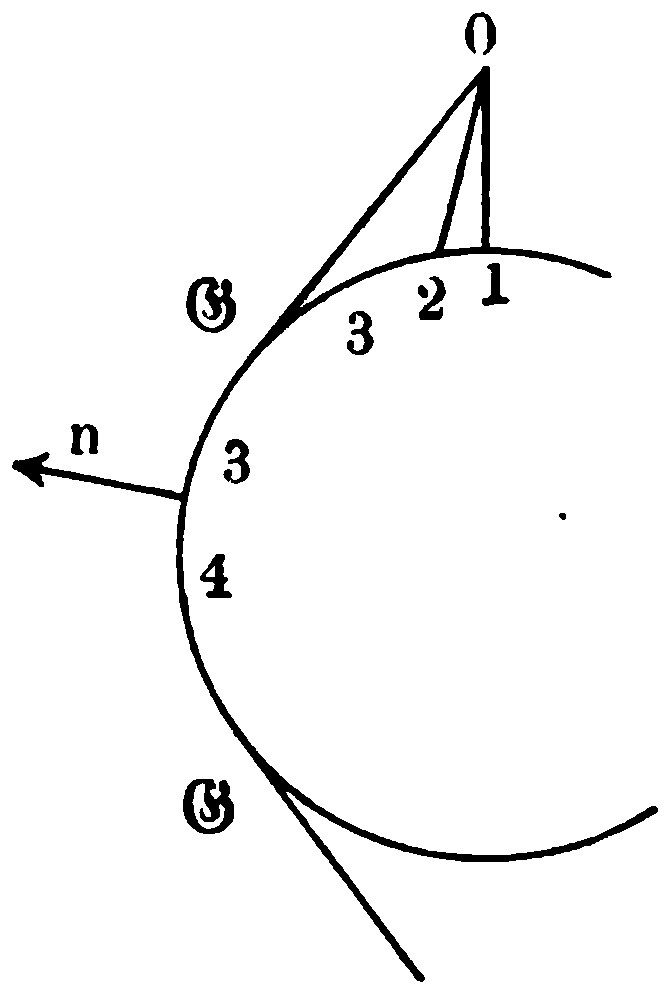
\includegraphics[width=.36\linewidth,height=48mm,keepaspectratio]{fig_assets/fig22_p0198_src_clean_x8.png}
\end{center}

Let an extremal meet the constraint (Fig.~22) at the point 1. On the former let the point 0 be so little removed from 1 that the arc 01 can be surrounded by a field whose extremals pass through the point 0. To this field also belong the parts of the constraint lying in the neighbourhood of the point 1, say as far as the point 2; and let the broken line 012 be a part of the combined curve which is to be examined for the occurrence of an extremum. Then, for the arc of the constraint belonging to the field, all that was proved in \S~20 for the curve $\Omega$ can be used. If $x$ and $y$ along the constraint are functions $\varphi(\tau)$ in the sense of \S~17, if $\tau$ increases in the direction 12, and if the point 3, moving along the constraint, passes through the position 1, then one has
\[
\frac{d(\overline{J}_{03}+\overline{J}_{32})}{d\tau}
=\mathfrak{E}\left(x,y,x',y',\frac{dx}{d\tau},\frac{dy}{d\tau}\right)\bigg|^3,
\]
where the quantities $x'$, $y'$ refer to the extremal 01 traversed in the direction from 0 toward 1. If therefore this quantity $\mathfrak{E}$ is different from zero, then the sum $\overline{J}_{03}+\overline{J}_{32}$, for arbitrarily small distance of the points 1 and 3, can become both greater and smaller than $\overline{J}_{01}+J_{12}$, and the latter quantity certainly forms no extremum of the integral $J$. If it is to be supplied by the polygonal line 012, the equation
\[
\mathfrak{E}\left(x,y,x',y',\frac{dx}{d\tau},\frac{dy}{d\tau}\right)\bigg|^1=0
\]
must therefore hold; that is, either extremal and constraint must touch one another in such a way that the direction of progress 012 changes continuously at the
% src-pdfpage=0199
point 1, or the quantity $\mathfrak{E}$ must vanish in an extraordinary manner.

A further necessary condition of the extremum is obtained by varying a piece 34 of the constraint belonging to the sought curve, in such a way that the endpoints are held fixed and the variations of the coordinates have the same properties as in \S~2. If one then puts
\[
\frac{F_x-F'_{x'}}{y'}=-\frac{F_y-F'_{y'}}{x'}=M,
\]
one obtains
\[
\delta J=\int M(y'\delta x-x'\delta y)\,dt,
\]
\[
\Delta J=\delta J+\int[\delta x,\delta y,\delta x',\delta y']_2\,dt.
\]
Here every point $(x+\delta x,y+\delta y)$ must belong to the region $\mathfrak{G}$ to which the sought curve is bound. Let $n$ denote the normal to the constraint pointing toward the interior of $\mathfrak{G}$, and $\varepsilon$ a positive constant. Then the stated requirements are fulfilled by the assumption
\[
\delta x=\varepsilon\cos(nx)(t-t_3)^3(t_4-t)^3,
\]
\[
\delta y=\varepsilon\cos(ny)(t-t_3)^3(t_4-t)^3,
\]
and one obtains
\[
\delta J=\varepsilon\int_3^4 [y'\cos(nx)-x'\cos(ny)]M(t-t_3)^3(t_4-t)^3\,dt,
\]
\[
\Delta J=\delta J+[\varepsilon]_2.
\]
Thus, if $\Delta J$ is to possess a fixed sign, the same must hold for the integral $\delta J:\varepsilon$ if it does not vanish. Since the points 3 and 4 can now be brought arbitrarily near one another, the quantity
\[
[y'\cos(nx)-x'\cos(ny)]M,
\]
if it does not vanish, must have the sign required of $\Delta J$, that is, in the case of a maximum it must be negative, and in the case of a minimum positive. Now the determinant
\[
\begin{vmatrix}
\cos(nx)&\cos(ny)\\
dx&dy
\end{vmatrix}
\]
is positive or negative according as the direction $n$, with respect to that of the element $(dx,dy)$, that is, to the direction of integration, lies in the same or the
% src-pdfpage=0200
opposite way as the $+x$-axis to the $+y$-axis; or, what is the same, according as the region $\mathfrak{G}$ is traversed in the negative or positive sense during the integration. In the first case it follows, if a maximum is to occur, that
\[
M\leqq 0,
\]
and if a minimum is sought, that
\[
M\geqq 0;
\]
in the second case these inequalities interchange their meaning.

\textbf{First example.} To draw between two points of the plane the shortest line which does not cross the constraints of a given region $\mathfrak{G}$.

The problem is of interest only when the straight line joining the two points cuts the constraint; then it is no longer the sought shortest connection, and one must consider combinations made of straight segments and parts of the constraint. Since
\[
F=\sqrt{x'^2+y'^2},\quad
M=\frac{1}{x'}\frac{d}{dt}\left(\frac{y'}{\sqrt{x'^2+y'^2}}\right),
\]
the quantity $\mathfrak{E}$ cannot vanish in an extraordinary manner; the straight segments must therefore touch the constraint where they meet it. If, further, $ds$ denotes an element of the constraint in the direction of integration, then one has
\[
M=\frac{1}{x'}\frac{d\cos(ds,y)}{dt}.
\]
If therefore $x'>0$, the orientation of the coordinate axes is as usual, and the first of the above cases occurs, that is, if the region $\mathfrak{G}$ lies to the right of a person advancing in the direction $ds$, then $\cos(ds,y)$ must increase in order that a minimum be possible; that is, the angle $(ds,y)$ decreases, $ds$ turns in the positive sense toward the left, and the concave side of the constraint lies toward the same side. Hence the constraint must be convex toward the interior of the enclosed region, insofar as it forms a part of a shortest connection. The same result is obtained for the other possible orientations of the figure.

Likewise, for a surface whose line element is represented in isometric coordinates, one easily finds, by means of the expression for the geodesic curvature used in \S~34, that
% src-pdfpage=0201
a constraint, where it belongs to a shortest connection, must turn its geodesically convex side toward the interior of the enclosed region; that is, the projection of the radius of curvature of the constraint onto the tangent plane of the surface points toward the outside of the region.

\textbf{Second example.} In Problem II (\S~9) it is evidently appropriate to seek the required curve only in the region $y\geqq 0$, and to regard the axis of rotation $y=0$ as a constraint; in general the latter is not cut by the extremals. But since one puts
\[
F=y\sqrt{x'^2+y'^2},
\]
the equations of the extremals
\[
F_x-\frac{d}{dt}\frac{yx'}{\sqrt{x'^2+y'^2}}=0,
\quad
F_y-F'_{y'}=\sqrt{x'^2+y'^2}-\frac{d}{dt}\left(\frac{yy'}{\sqrt{x'^2+y'^2}}\right)=0
\]
are satisfied by the assumption
\[
x'=0,
\]
so that the straight lines $x=\mathrm{const.}$ are also to be regarded as extremals. On the $y$-axis the quantity $\mathfrak{E}$ vanishes, for arbitrary direction of the arc elements determining it, and therefore in an extraordinary manner, since it has the factor $y$; further, for $y=0$, $x'>0$, the equation
\begin{equation}\tag{5}
M=-\frac{1}{x'}(F_y-F'_{y'})=-1
\end{equation}
holds. If one now integrates along the $x$-axis in the direction of increasing $x$, the region $\mathfrak{G}$ is traversed in the positive sense, and the second of the cases distinguished above occurs; the condition for the minimum relating to $M$ is therefore fulfilled. Hence, as a discontinuous solution of the problem, one may consider the broken line which consists of a piece of the axis of rotation and two positive ordinates of arbitrary length erected at its endpoints; that is, for this polygonal line the necessary conditions of the minimum that have been considered are fulfilled.

\begin{center}
{\small Fig. 23.}\par\vspace{1mm}
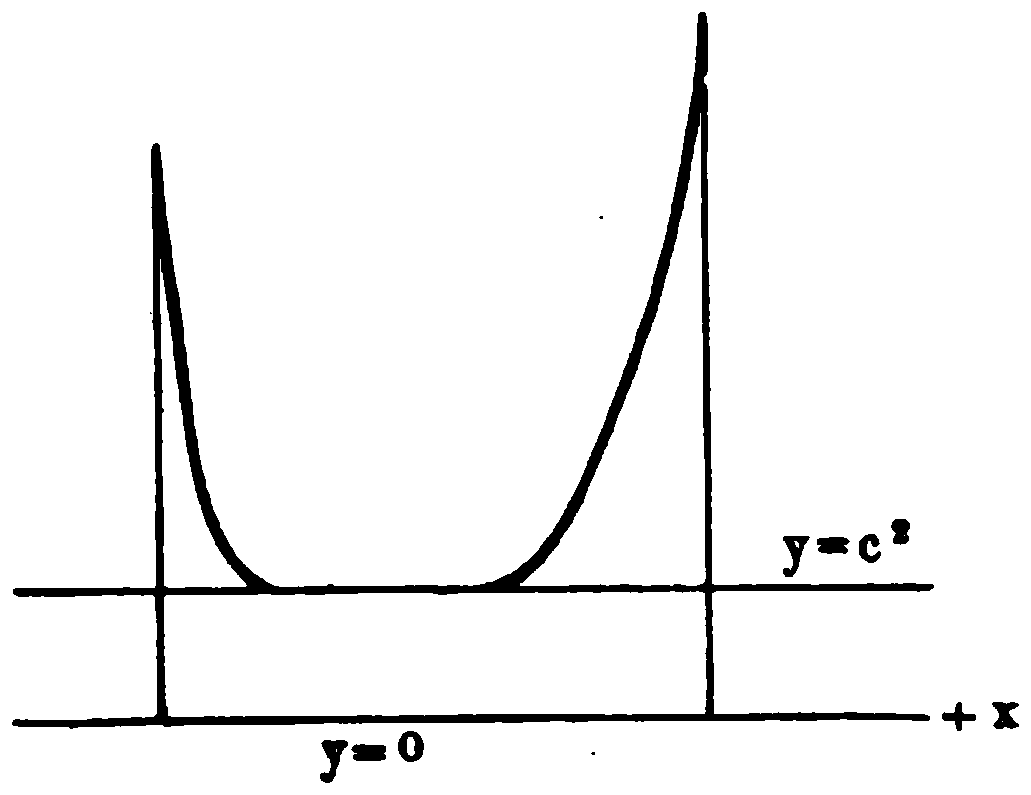
\includegraphics[width=.48\linewidth,height=42mm,keepaspectratio]{fig_assets/fig23_p0201_src_clean_x8.png}
\end{center}

Two points of the half-plane $y>0$ can always be joined by a broken line of the stated nature,
% src-pdfpage=0202
but by no means always by an arc of an extremal; from this it is evident that the solution of the extremum problem is advanced by introducing the broken line.

If one introduces a straight line $y=c^2$ as constraint (Fig.~23, p.~179), and if $y-c^2$ is positive for the given points, then for the constraint traversed in the direction of increasing $x$ equation (5) holds, while the quantity $\mathfrak{E}$ can vanish only in the ordinary manner. The sought line must therefore now be composed of pieces of the straight line $y=c^2$ and of arcs of catenaries touching it, which have not degenerated into the straight lines $x=\mathrm{const.}$.

\begin{center}
{\large \S~45.}
\end{center}

Let, as in the fourth section, the integral
\[
J=\int Fdt
\]
be made an extremum for a prescribed value of the integral
\[
K=\int Gdt.
\]
Along an extremal $\mathfrak{C}$ passing through the point 1, let $y$ be representable in its neighbourhood as a regular function of $x$, and let the quantity
\[
F_{y'y'}+\lambda G_{y'y'}=x'^2H_1
\]
be different from zero. Then, by \S~27, the totality of all extremals in the neighbourhood of the point 1 and of the curve $\mathfrak{C}$ can be represented in the form
\[
y=\Phi(x,a,b,\lambda),
\]
and the function $\Phi$ is regular in a neighbourhood of the value system $(x_1,a^0,b^0,\lambda^0)$ defined by the curve $\mathfrak{C}$. In particular, consider all extremals which pass through 1 and through one further point 0 belonging to the curve $\mathfrak{C}$, so that the equations
\begin{equation}\tag{6}
y_1=\Phi(x_1,a,b,\lambda),\quad y_0=\Phi(x_0,a,b,\lambda)
\end{equation}
define the quantities $a$ and $b$ as functions of $\lambda$, as soon as the determinant
\[
\Psi(x_0,x_1,a^0,b^0,\lambda^0)=
\begin{vmatrix}
\Phi_a(x_1,a^0,b^0,\lambda^0)&\Phi_b(x_1,a^0,b^0,\lambda^0)\\
\Phi_a(x_0,a^0,b^0,\lambda^0)&\Phi_b(x_0,a^0,b^0,\lambda^0)
\end{vmatrix}
\]
% src-pdfpage=0203
is different from zero. Since one can now evidently put
\[
\Phi(x,a,b,\lambda)=y_1+a+b(x-x_1)+[x-x_1]_2,
\]
it follows that
\[
\Phi_a(x,a,b,\lambda)=1+[x-x_1]_2,
\quad
\Phi_b(x,a,b,\lambda)=x-x_1+[x-x_1]_2;
\]
that determinant therefore takes the form
\[
\begin{vmatrix}
1&0\\
1+[x_0-x_1]_2&x_0-x_1+[x_0-x_1]_2
\end{vmatrix},
\]
and is different from zero as soon as the quantity $|x_1-x_0|$ is sufficiently small. Then equations (6) give
\[
0=\Phi_a(x_1,a,b,\lambda)\frac{da}{d\lambda}
+\Phi_b(x_1,a,b,\lambda)\frac{db}{d\lambda}
+\Phi_\lambda(x_1,a,b,\lambda),
\]
\[
0=\Phi_a(x_0,a,b,\lambda)\frac{da}{d\lambda}
+\Phi_b(x_0,a,b,\lambda)\frac{db}{d\lambda}
+\Phi_\lambda(x_0,a,b,\lambda),
\]
and furthermore one plainly has to regard $\overline{K}_{01}$ as a function of $\lambda$ for which the equation
\[
\frac{d\overline{K}_{01}}{d\lambda}
=\frac{\partial\overline{K}_{01}}{\partial a}\frac{da}{d\lambda}
+\frac{\partial\overline{K}_{01}}{\partial b}\frac{db}{d\lambda}
+\frac{\partial\overline{K}_{01}}{\partial\lambda}
\]
holds, when the partial derivatives are formed on the assumption that $x_0$ and $x_1$, but not $y_0$ and $y_1$, are kept fixed. From this follows
\[
0=\begin{vmatrix}
\Phi_a(x_0,a,b,\lambda)&\Phi_b(x_0,a,b,\lambda)&\Phi_\lambda(x_0,a,b,\lambda)\\
\Phi_a(x_1,a,b,\lambda)&\Phi_b(x_1,a,b,\lambda)&\Phi_\lambda(x_1,a,b,\lambda)\\
\dfrac{\partial\overline{K}_{01}}{\partial a}&\dfrac{\partial\overline{K}_{01}}{\partial b}&\dfrac{\partial\overline{K}_{01}}{\partial\lambda}-\dfrac{d\overline{K}_{01}}{d\lambda}
\end{vmatrix}
\]
or
\[
\Delta(x_0,x_1)=\frac{d\overline{K}_{01}}{d\lambda}\cdot\Psi(x_0,x_1,a,b,\lambda).
\]
The left-hand side of this equation is, by \S~42, different from zero as soon as the distance of the points 0 and 1 has become sufficiently small and one puts
\begin{equation}\tag{7}
a=a^0,
\quad b=b^0,
\quad \lambda=\lambda^0;
\end{equation}
then the quantity $\Psi$ is finite, and it follows that
\begin{equation}\tag{8}
0\gtrless \frac{d\overline{K}_{01}}{d\lambda}\bigg|^{a=a^0,\,b=b^0,\,\lambda=\lambda^0}.
\end{equation}
Now plainly
% src-pdfpage=0204
\[
\begin{aligned}
\frac{d\overline{K}_{01}}{d\lambda}
&=\frac{d}{d\lambda}\int_{x_0}^{x_1}g(x,y,p)\,dx \\
&=\int_{x_0}^{x_1}\left\{g_y\left(\Phi_a\frac{da}{d\lambda}+\Phi_b\frac{db}{d\lambda}+\Phi_\lambda\right)\right.\\
&\hspace{18mm}\left.+g_p\frac{d}{dx}\left(\Phi_a\frac{da}{d\lambda}+\Phi_b\frac{db}{d\lambda}+\Phi_\lambda\right)\right\}\,dx \\
&=g_p\left(\Phi_a\frac{da}{d\lambda}+\Phi_b\frac{db}{d\lambda}+\Phi_\lambda\right)\bigg|_{x_0}^{x_1}\\
&\hspace{10mm}+\int_{x_0}^{x_1}\left(g_y-\frac{dg_p}{dx}\right)
\left(\Phi_a\frac{da}{d\lambda}+\Phi_b\frac{db}{d\lambda}+\Phi_\lambda\right)\,dx \\
&=\int_{x_0}^{x_1}\left(g_y-\frac{dg_p}{dx}\right)
\left(\Phi_a\frac{da}{d\lambda}+\Phi_b\frac{db}{d\lambda}+\Phi_\lambda\right)\,dx.
\end{aligned}
\]
and similarly
\[
\frac{d\overline{J}_{01}}{d\lambda}
=\int_{x_0}^{x_1}\left(f_y-\frac{df_p}{dx}\right)
\left(\Phi_a\frac{da}{d\lambda}+\Phi_b\frac{db}{d\lambda}+\Phi_\lambda\right)\,dx;
\]
since, moreover, for every extremal an equation
\[
f_y-\frac{df_p}{dx}+\lambda\left(g_y-\frac{dg_p}{dx}\right)=0
\]
holds, one obtains
\begin{equation}\tag{9}
-\frac{d\overline{J}_{01}}{d\lambda}=\lambda\frac{d\overline{K}_{01}}{d\lambda},
\end{equation}
and since we suppose $\lambda$ different from zero, the left-hand side of this equation is also different from zero under assumption (7). Moreover the expansions
\[
\overline{J}_{01}(\lambda)=\overline{J}_{01}(\lambda^0)+(\lambda-\lambda^0)\left(\frac{d\overline{J}_{01}}{d\lambda}\right)_{\lambda=\lambda^0}+[\lambda-\lambda^0]_2,
\]
\[
\overline{K}_{01}(\lambda)=\overline{K}_{01}(\lambda^0)+(\lambda-\lambda^0)\left(\frac{d\overline{K}_{01}}{d\lambda}\right)_{\lambda=\lambda^0}+[\lambda-\lambda^0]_2
\]
plainly hold. This whole consideration is repeated for a second extremal $\mathfrak{C}_1$, on which the points 2 and 3 lie. The value of $\lambda$ belonging to it we denote by $\lambda_+^0$; for the sake of symmetry, we put $\lambda_-$ for $\lambda$ in the preceding formulae and in general denote by the appended signs $-$ and $+$ whether a quantity is to refer to the curve $\mathfrak{C}$ or $\mathfrak{C}_1$. One then obtains the equations
% src-pdfpage=0205
\[
\overline{J}_{23}(\lambda_+)=\overline{J}_{23}(\lambda_+^0)+
(\lambda_+-\lambda_+^0)\left(\frac{d\overline{J}_{23}}{d\lambda_+}\right)_{\lambda_+=\lambda_+^0}
+[\lambda_+-\lambda_+^0]_2,
\]
\[
\overline{K}_{23}(\lambda_+)=\overline{K}_{23}(\lambda_+^0)+
(\lambda_+-\lambda_+^0)\left(\frac{d\overline{K}_{23}}{d\lambda_+}\right)_{\lambda_+=\lambda_+^0}
+[\lambda_+-\lambda_+^0]_2.
\]
Now assume that the curves $\mathfrak{C}$ and $\mathfrak{C}_1$ are parts of a polygonal line composed in some way which, without having the continuity properties of the curve $\mathfrak{B}$ considered in \S~2, makes the integral $J$ an extremum for a prescribed value of $K$. Then vary in such a way that the arcs 23 and 01 of the curves $\mathfrak{C}_1$ and $\mathfrak{C}$ are replaced by other extremal arcs with the same endpoints, for which the preceding notations may remain valid. Since the integral $K$ is to have, along the varied line, the same value as along the original one, one has
\[
\overline{K}_{01}(\lambda_-)+\overline{K}_{23}(\lambda_+)
=\overline{K}_{01}(\lambda_-^0)+\overline{K}_{23}(\lambda_+^0),
\]
and the quantities $\lambda_-$, $\lambda_+$ are therefore connected by the following relation:
\[
0=(\lambda_- -\lambda_-^0)\left(\frac{d\overline{K}_{01}}{d\lambda_-}\right)_{\lambda_- =\lambda_-^0}
+(\lambda_+ -\lambda_+^0)\left(\frac{d\overline{K}_{23}}{d\lambda_+}\right)_{\lambda_+ =\lambda_+^0}
+[\lambda_- -\lambda_-^0,\lambda_+ -\lambda_+^0]_2.
\]
The extremum requires that the quantity
\[
\overline{J}_{01}(\lambda_-)+\overline{J}_{23}(\lambda_+)-\overline{J}_{01}(\lambda_-^0)-\overline{J}_{23}(\lambda_+^0)
\]
have a fixed sign. Since it can be represented in the form
\[
(\lambda_- -\lambda_-^0)\left(\frac{d\overline{J}_{01}}{d\lambda_-}\right)_{\lambda_- =\lambda_-^0}
+(\lambda_+ -\lambda_+^0)\left(\frac{d\overline{J}_{23}}{d\lambda_+}\right)_{\lambda_+ =\lambda_+^0}
\]
\[
+[\lambda_+ -\lambda_+^0,\lambda_- -\lambda_-^0]_2,
\]
the general theorem of \S~7 gives
\[
0=
\begin{vmatrix}
\dfrac{d\overline{J}_{01}}{d\lambda_-}&\dfrac{d\overline{J}_{23}}{d\lambda_+}\\[1.2ex]
\dfrac{d\overline{K}_{01}}{d\lambda_-}&\dfrac{d\overline{K}_{23}}{d\lambda_+}
\end{vmatrix}
\]
for $\lambda_- =\lambda_-^0$, $\lambda_+ =\lambda_+^0$. From this it follows, by relations (8), (9) and the analogous ones referring to the curve 23, that
\[
0=\frac{d\overline{K}_{01}}{d\lambda_-}\frac{d\overline{K}_{23}}{d\lambda_+}
\begin{vmatrix}
\lambda_-^0&\lambda_+^0\\
1&1
\end{vmatrix},
\quad \lambda_-^0=\lambda_+^0.
\]
% src-pdfpage=0206
This equation expresses the simplest case of the law, set up by \textsc{Mayer}, of the conservation of the isoperimetric constant, which according to the result obtained has the same value for $\mathfrak{C}$ and $\mathfrak{C}_1$.

\textbf{Example.} Between the points 0 and 2, draw a line of given length which passes through the given point 1 and encloses with the straight segment 02 the greatest possible area.

If the sought curve has no discontinuity between 0 and 1, nor between 1 and 2, then the arcs 01 and 12 must be extremals, and hence circles, by the considerations which gave the corresponding result in \S~43. According to the theorem obtained, the sought line necessarily consists of two circular arcs 01, 12 of equal radius. If one allows this radius to vary, it is readily seen that, within certain limits, the total length of the two arcs can assume every value.

% machine-unit: Kneser_LVR_EN_p0206_p0219 §§46-48
% src-pdfpage=0206
% src-break=0206
\begin{center}
{\large \S~46.}
\end{center}

Let the extremals $\mathfrak C$ and $\mathfrak C_1$ now have the point 1 in common; let the points 0 and 2 be taken so near the point 1 that the extremals passing through the former surround every part of the arc 01, and the extremals passing through the latter surround every part of the arc 12, as a field; this is possible by \S~41 if $H_1$ does not vanish along the arcs 01 and 12 (Fig.~21, p.~172). If the two fields are represented by the systems of equations
\[
 x=\xi_-(t_-,a_-,b_-),\quad y=\eta_-(t_-,a_-,b_-),
\]
\[
 x=\xi_+(t_+,a_+,b_+),\quad y=\eta_+(t_+,a_+,b_+),
\]
then every point 3 sufficiently little different from 1 can be connected with 0 and 2 by extremals of the fields. If one regards the point 3 as variable in the neighbourhood of the position 1, then one obtains (\S~35)
\begin{equation}\tag{10}
\frac{\partial\overline K_{03}}{\partial t_-}=G_-\bigg|^3,
\quad
\frac{\partial\overline K_{03}}{\partial a_-}
=\int_0^3\bigl[\xi_a(G_x-G_{x'}')+\eta_a(G_y-G_{y'}')\bigr]_-\,dt_-
+\bigl(\xi_aG_{x'}+\eta_aG_{y'}\bigr)_-\bigg|^3
\end{equation}
together with an analogous formula in which $a$ is replaced by $b$; if therefore the increments $\delta t_-$, $\delta a_-$, $\delta b_-$ correspond to the passage from the point 1 to 3 and from the arc 01 to 03, then
% src-pdfpage=0207
\[
\overline K_{03}-\overline K_{01}=\Delta\overline K_{01}
=G_{x'}^-\delta x+G_{y'}^-\delta y\bigg|^1
+A_-\delta a_-+B_-\delta b_-+[\delta t_-,\delta a_-,\delta b_-]_2,
\]
where it is put that
\begin{equation}\tag{11}
\delta x=(\xi_a\delta a+\xi_b\delta b+\xi_t\delta t)_-,
\quad
\delta y=(\eta_a\delta a+\eta_b\delta b+\eta_t\delta t)_-,
\end{equation}
\[
A_- =\int_0^1\bigl[\xi_a(G_x-G_{x'}')+\eta_a(G_y-G_{y'}')\bigr]_-\,dt_-
\]
and $B_-$ arises from $A_-$ by replacing $a$ by $b$. Analogously one obtains
\[
\Delta\overline K_{12}
=-G_{x'}^+\delta x-G_{y'}^+\delta y\bigg|^1
+A_+\delta a_+ +B_+\delta b_+ +[\delta t_+,\delta a_+,\delta b_+]_2,
\]
where the quantities $\delta t_+$, $\delta a_+$, $\delta b_+$, $A_+$, $\ldots$ have for the extremal 12 the meaning analogous to that which $\delta t_-$, $\ldots$ have for 01, so that
\begin{equation}\tag{12}
\delta x=(\xi_a\delta a+\xi_b\delta b+\xi_t\delta t)_+,
\quad
\delta y=(\eta_a\delta a+\eta_b\delta b+\eta_t\delta t)_+.
\end{equation}
If now $J$ is to become an extremum for a given value of $K$, then the broken line consisting of the extremal arcs 03, 32 is an admissible variation of the broken line 012 as soon as the eight quantities $\delta x$, $\delta y$, $\delta a_\pm$, $\delta b_\pm$, $\delta t_\pm$ are so determined that the equation
\[
\Delta\overline K_{01}+\Delta\overline K_{12}=0
\]
holds, or
\begin{equation}\tag{13}
\begin{aligned}
0={}&(G_{x'}^- -G_{x'}^+)\delta x+(G_{y'}^- -G_{y'}^+)\delta y\bigg|^1 \\
&+A_-\delta a_-+B_-\delta b_-+A_+\delta a_+ +B_+\delta b_+ \\
&+[\delta a_+,\delta b_+,\delta t_+,\delta a_-,\delta b_-,\delta t_-]_2.
\end{aligned}
\end{equation}
This equation, in conjunction with those given under (11) and (12), can serve to express five of the eight quantities $\delta$ by means of the three remaining ones. If, for instance, one takes for the latter $\delta x$, $\delta y$, $\delta a_+$, then the determinant of the terms linear in the quantities $\delta t_-$, $\delta a_-$, $\delta b_-$, $\delta t_+$, $\delta b_+$ on the right hand sides of the five equations in question is
% src-pdfpage=0208
\begin{equation}\tag{14}
\begin{vmatrix}
0&A_-&B_-&0&B_+\\
\xi_t^-&\xi_a^-&\xi_b^-&0&0\\
\eta_t^-&\eta_a^-&\eta_b^-&0&0\\
0&0&0&\xi_t^+&\xi_b^+\\
0&0&0&\eta_t^+&\eta_b^+
\end{vmatrix}
=
\begin{vmatrix}
0&A_-&B_-\\
\xi_t^-&\xi_a^-&\xi_b^-\\
\eta_t^-&\eta_a^-&\eta_b^-
\end{vmatrix}
\left[\frac{\partial(\xi,\eta)}{\partial(t,b)}\right]_+ .
\end{equation}
If in the first determinant on the right one adds the second and third horizontal rows, multiplied by $G_{x'}^-$ and $G_{y'}^-$, to the first row, and bears in mind that the derivatives of $\xi$ and $\eta$, as in equations (11), refer to the point 1, then equations (10) show that the determinant has the value
\[
\frac{\partial(\overline K_{01},\xi_-,\eta_-)}{\partial(t_-,a_-,b_-)}
\]
that is, that it is equal to the quantity $\Delta_-$ belonging to the field of the arc 01, and is therefore different from zero. Since furthermore the arc 12 is also surrounded by a field for which the quantity
\[
\frac{\partial(\xi_+,\eta_+,\overline K_{21})}{\partial(t_+,a_+,b_+)}
\]
does not vanish, the quantities
\[
\left[\frac{\partial(\xi,\eta)}{\partial(t,a)}\right]_+,
\quad
\left[\frac{\partial(\xi,\eta)}{\partial(t,b)}\right]_+
\]
are not both zero by \S~35; hence either the second factor on the right hand side of equation (14) is also different from zero, or this is achieved by interchanging $a_+$ and $b_+$. Thus one can always express five of the quantities $\delta$ by the other three, among which $\delta x$ and $\delta y$ occur, as power series in these three arguments.

If now, in the expressions $A$, $B$, one replaces the functional symbol $G$ by $F$, one obtains $\mathfrak A$, $\mathfrak B$; the equation of the extremals then gives
\begin{equation}\tag{15}
\lambda_-A_-+\mathfrak A_-=
\lambda_-B_-+\mathfrak B_-=
\lambda_+A_+ +\mathfrak A_+=
\lambda_+B_+ +\mathfrak B_+=0,
\end{equation}
and by the preceding paragraph one has for $\mathfrak C$ and $\mathfrak C_1$
\[
\lambda_+=\lambda_-=\lambda.
\]
Further, analogously to the expression $\Delta\overline K_{01}+\Delta\overline K_{12}$ developed in equation (13), one obtains
% src-pdfpage=0209
\[
\begin{aligned}
\Delta\overline J_{01}+\Delta\overline J_{12}
={}&(F_{x'}^- -F_{x'}^+)\delta x+(F_{y'}^- -F_{y'}^+)\delta y\bigg|^1\\
&+\mathfrak A_-\delta a_-+\mathfrak B_-\delta b_-+\mathfrak A_+\delta a_+ +\mathfrak B_+\delta b_+ \\
&+[\delta a_\pm,\delta b_\pm,\delta t_\pm]_2;
\end{aligned}
\]
if therefore one multiplies equation (13) by $\lambda$ and adds it to the last expression, then, since $H=F+\lambda G$, it follows from (15) that
\[
\Delta\overline J_{01}+\Delta\overline J_{12}
=(H_{x'}^- -H_{x'}^+)\delta x+(H_{y'}^- -H_{y'}^+)\delta y\bigg|^1
+[\delta a_\pm,\delta b_\pm,\delta t_\pm]_2.
\]
This quantity, if the required extremum is present, must have a fixed sign under the conditions (11), (12), (13); since here only the quantities $\delta x$, $\delta y$ occur in the linear terms, \S~7 gives for the point 1
\begin{equation}\tag{16}
(H_{x'}^- -H_{x'}^+)\delta x+(H_{y'}^- -H_{y'}^+)\delta y=0.
\end{equation}
According as the point 1 is freely movable or is bound to the curve
\[
h(x,y)=0,
\]
one obtains the relations
\[
H_{x'}^- -H_{x'}^+=H_{y'}^- -H_{y'}^+=0
\]
or
\[
\begin{vmatrix}
H_{x'}^- -H_{x'}^+&H_{y'}^- -H_{y'}^+\\
h_x&h_y
\end{vmatrix}=0.
\]
Thus exactly the same restrictions hold for a corner point as, according to \S~43, in the case of the absolute extremum, when $F$ is replaced by $F+\lambda G$.

\textbf{Example. Problem IX} (\S~34). One has
\[
H=yx' +\lambda\sqrt{x'^2+y'^2},
\]
\[
H_{x'}=y+\frac{\lambda x'}{\sqrt{x'^2+y'^2}},
\quad
H_{y'}=\frac{\lambda y'}{\sqrt{x'^2+y'^2}};
\]
therefore equation (16) gives
\begin{equation}\tag{17}
\lambda\left(\frac{x'\delta x+y'\delta y}{\sqrt{x'^2+y'^2}}\right)_-
=
\lambda\left(\frac{x'\delta x+y'\delta y}{\sqrt{x'^2+y'^2}}\right)_+.
\end{equation}
Since now $\lambda$ is different from zero, a freely available corner would imply
\[
\left(\frac{x'}{\sqrt{x'^2+y'^2}}\right)_-
=
\left(\frac{x'}{\sqrt{x'^2+y'^2}}\right)_+,
\quad
\left(\frac{y'}{\sqrt{x'^2+y'^2}}\right)_-
=
\left(\frac{y'}{\sqrt{x'^2+y'^2}}\right)_+,
\]
% src-pdfpage=0210
that is, the directions of the extremals 01 and 12 would agree at the point 1, so that no discontinuity would occur. If, on the other hand, the point 1 is bound to a curve $\mathfrak K$, whose arc element is $Ds$, and if at the point 1 we denote by $-$, $+$ the directions of the extremal 01 from 0 toward 1 and of the extremal 12 from 1 toward 2, then equation (17) gives
\[
\cos(Ds,-)=\cos(Ds,+).
\]
The arcs 01 and 12 therefore lie on the same side of the curve $\mathfrak K$ and form with its tangent equal acute angles, opened toward different sides, that is, they lie like the incident and reflected ray of light.

Thus, for example, if from the given point 5 to an unspecified point 1 of the curve $\mathfrak K$, and back again to the point 5, a closed line of given length is to be drawn which encloses the greatest possible area, it must consist of two circular arcs of the same radius, which form equal angles with the curve $\mathfrak K$ in the stated sense.

\begin{center}
{\large \S~47.}
\end{center}

It remains to investigate when a polygonal line 0123 can occur in the solution of the isoperimetric problem, when the compared curves are bound to a region $\mathfrak G$ bounded by constraints, and the segment 12 belongs to a constraint whereas the arcs 01 and 23 do not, so that the latter, by \S~45, are extremals with the same isoperimetric constant. Then let (Fig.~24) the points 0 and 3 be taken so near to 1 and 2 that the arcs 01 and 23 can be surrounded by fields whose extremals pass through 0 and 3. Near the points 1 and 2 let the points 4 and 5 lie on the constraint; then there are extremals 04 and 53 which belong to the two fields, and the polygonal line 0453 is an admissible variation of the polygonal line 0123 if
\[
\overline K_{01}+K_{12}+\overline K_{23}=\overline K_{04}+K_{45}+\overline K_{53},
\]
or
\begin{equation}\tag{18}
K_{12}-K_{45}=\Delta\overline K_{01}+\Delta\overline K_{23},
\end{equation}
\begin{center}
{\small Fig. 24.}\par\vspace{1mm}
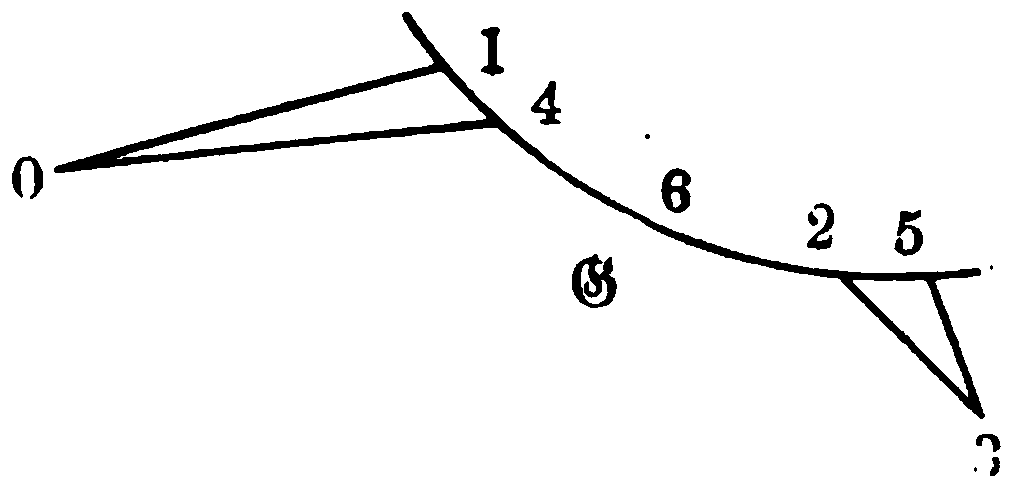
\includegraphics[width=.48\linewidth,height=42mm,keepaspectratio]{fig_assets/fig24_p0210_src_clean_x8.png}
\end{center}
% src-pdfpage=0211
where the unprimed integrals always refer to the constraint, and the signs $\Delta$ denote the increment in the passage from 01 and 23 to 04 and 53. To discuss this requirement, we assign to the symbols $\xi$, $\eta$, $t_+$, $a_\pm$, $b_\pm$, $A_\pm$, $\delta t_\pm\ldots$ the same meaning for the arcs 01 and 23 that they had in the preceding paragraph for 01 and 12, so that the sign $-$ belongs to the first of the denoted arcs, and the sign $+$ to the second; accordingly let
\[
\begin{aligned}
\delta x_-+[\delta t_-,\delta a_-,\delta b_-]_2&=x_4-x_1,\\
\delta y_-+[\delta t_-,\delta a_-,\delta b_-]_2&=y_4-y_1,\\
\delta x_++[\delta t_+,\delta a_+,\delta b_+]_2&=x_5-x_2,\\
\delta y_++[\delta t_+,\delta a_+,\delta b_+]_2&=y_5-y_2,
\end{aligned}
\]
and let the expressions $\delta x$, $\delta y$ be linear with respect to $\delta t$, $\delta a$, $\delta b$. The right hand side of equation (18) is then found from the formulae established in \S~46 for $K_{01}$; namely one has
\begin{equation}\tag{19}
\begin{aligned}
\Delta\overline K_{01}&=G_{x'}^-\delta x_-+G_{y'}^-\delta y_-\bigg|^1
+A_-\delta a_-+B_-\delta b_-+[\delta t_-,\delta a_-,\delta b_-]_2,\\
\Delta\overline K_{23}&=-G_{x'}^+\delta x_+ -G_{y'}^+\delta y_+\bigg|^2
+A_+\delta a_+ +B_+\delta b_+ +[\delta t_+,\delta a_+,\delta b_+]_2;
\end{aligned}
\end{equation}
and between the quantities $\delta$ there now hold the four relations
\begin{equation}\tag{20}
\delta x_\pm=(\xi_t\delta t+\xi_a\delta a+\xi_b\delta b)_\pm,
\quad
\delta y_\pm=(\eta_t\delta t+\eta_a\delta a+\eta_b\delta b)_\pm,
\end{equation}
where either the upper, or on both sides the lower, of the signs $\pm$ is to be taken. If therefore here and in equation (18) the quantities $\delta t_-$, $\delta a_-$, $\delta b_-$, $\delta b_+$, $\delta t_+$ are regarded as determined by the remaining quantities $\delta$, then the terms containing those five quantities in the five equations set up have exactly the same determinant as in equations (11), (12), (13) of the preceding paragraph. The proof given there that this determinant, or the one obtained by interchanging $a_+$ and $b_+$, is different from zero remains valid when the arc 12 considered there is replaced by 23. The five equations (18), (20) can therefore be solved for the quantities $\delta t_\pm$, $\delta a_-$, $\delta b_\pm$ as soon as $K_{12}-K_{45}$ is sufficiently small.

% src-pdfpage=0212
Now let $x$ and $y$ along the constraint, near the points 1 and 2, be regular functions of the parameters $\tau_-$, $\tau_+$, which increase in the direction 12 and receive, in the passage to 4 and 5, the increments $D\tau_-$ and $D\tau_+$; then
\[
\delta x_- =\frac{dx}{d\tau_-}\bigg|^1D\tau_-+[D\tau_-]_2,
\quad
\delta y_- =\frac{dy}{d\tau_-}\bigg|^1D\tau_-+[D\tau_-]_2,
\]
and similar equations hold at the point 2. If one furthermore supposes that the integrands $F$ and $G$ are regular in the neighbourhood of every element of the polygonal line 0123, then for positive values $D\tau_-$
\begin{equation}\tag{21}
K_{14}=G\left(x,y,\frac{dx}{d\tau_-},\frac{dy}{d\tau_-}\right)\bigg|^1D\tau_-+[D\tau_-]_2,
\end{equation}
and for negative values
\begin{equation}\tag{22}
K_{41}=G\left(x,y,\frac{dx}{d\tau_-},\frac{dy}{d\tau_-}\right)\bigg|^1(-D\tau_-)+[D\tau_-]_2.
\end{equation}
If now, on the constraint, the point 6 is fixed arbitrarily between 1 and 2 and outside the segments 14, 25, then, according as $D\tau_-$ is positive or negative, one has one or the other of the equations
\[
K_{46}-K_{16}=-K_{14},
\quad
K_{46}-K_{16}=K_{41};
\]
in every case therefore, by (21), (22),
\begin{equation}\tag{23}
\Delta K_{16}=K_{46}-K_{16}
=-G\left(x,y,\frac{dx}{d\tau_-},\frac{dy}{d\tau_-}\right)\bigg|^1D\tau_-+[D\tau_-]_2.
\end{equation}
In a similar manner one obtains
\begin{equation}\tag{24}
\Delta K_{62}=K_{65}-K_{62}
=+G\left(x,y,\frac{dx}{d\tau_+},\frac{dy}{d\tau_+}\right)\bigg|^2D\tau_+ +[D\tau_+]_2;
\end{equation}
if the sum of these expressions,
\[
\Delta K_{16}+\Delta K_{62}=\Delta K_{12}=K_{45}-K_{12},
\]
is substituted into equation (18), then from (19) it follows that
\begin{equation}\tag{25}
\begin{aligned}
&G\left(x,y,\frac{dx}{d\tau_-},\frac{dy}{d\tau_-}\right)\bigg|^1D\tau_-
-G\left(x,y,\frac{dx}{d\tau_+},\frac{dy}{d\tau_+}\right)\bigg|^2D\tau_+\\
&\quad=G_{x'}^-\frac{dx}{d\tau_-}+G_{y'}^-\frac{dy}{d\tau_-}\bigg|^1D\tau_-
-G_{x'}^+\frac{dx}{d\tau_+}-G_{y'}^+\frac{dy}{d\tau_+}\bigg|^2D\tau_+\\
&\qquad +A_-\delta a_-+B_-\delta b_-+A_+\delta a_+ +B_+\delta b_+
+[\delta a_\pm,\delta b_\pm,\delta t_\pm,D\tau_\pm]_2.
\end{aligned}
\end{equation}

% src-pdfpage=0213
The right hand sides of equations (19) pass into $\Delta\overline J_{01}$ and $\Delta\overline J_{23}$ when $G$ is replaced by $F$, and $A$ and $B$ by $\mathfrak A$ and $\mathfrak B$; if therefore one multiplies the last equation by the constant $\lambda$ belonging to both curves 01 and 23, and takes equations (15) into account, one obtains
\[
\begin{aligned}
&\Delta\overline J_{01}+\Delta\overline J_{23}
+\lambda G\left(x,y,\frac{dx}{d\tau_-},\frac{dy}{d\tau_-}\right)\bigg|^1D\tau_-\\
&\quad -\lambda G\left(x,y,\frac{dx}{d\tau_+},\frac{dy}{d\tau_+}\right)\bigg|^2D\tau_+\\
&=H_{x'}^-\frac{dx}{d\tau_-}+H_{y'}^-\frac{dy}{d\tau_-}\bigg|^1D\tau_-
-H_{x'}^+\frac{dx}{d\tau_+}-H_{y'}^+\frac{dy}{d\tau_+}\bigg|^2D\tau_+\\
&\quad +[\delta a_\pm,\delta b_\pm,\delta t_\pm,D\tau_\pm]_2.
\end{aligned}
\]
Now the integral $J_{0123}$ receives, under the variation considered, the increment
\[
\Delta\overline J_{01}+\Delta\overline J_{23}+J_{45}-J_{12}
=\Delta\overline J_{01}+\Delta\overline J_{23}+\Delta J_{16}+\Delta J_{62};
\]
since furthermore, analogously to equations (23), (24), one may put
\[
\Delta J_{16}=-F\left(x,y,\frac{dx}{d\tau_-},\frac{dy}{d\tau_-}\right)\bigg|^1D\tau_-+[D\tau_-]_2,
\]
\[
\Delta J_{62}=F\left(x,y,\frac{dx}{d\tau_+},\frac{dy}{d\tau_+}\right)\bigg|^2D\tau_+ +[D\tau_+]_2,
\]
one obtains for that increment the expression
\[
\begin{aligned}
&H_{x'}^-\frac{dx}{d\tau_-}+H_{y'}^-\frac{dy}{d\tau_-}
-H\left(x,y,\frac{dx}{d\tau_-},\frac{dy}{d\tau_-}\right)\bigg|^1D\tau_-\\
&\quad -H_{x'}^+\frac{dx}{d\tau_+}-H_{y'}^+\frac{dy}{d\tau_+}
+H\left(x,y,\frac{dx}{d\tau_+},\frac{dy}{d\tau_+}\right)\bigg|^2D\tau_+\\
&\quad +[\delta t_\pm,\delta a_\pm,\delta b_\pm,D\tau_\pm]_2,
\end{aligned}
\]
or briefly
\[
\Delta J_{0123}=\mathfrak E^-D\tau_- -\mathfrak E^+D\tau_+ +[\delta t_\pm,\delta a_\pm,\delta b_\pm,D\tau_\pm]_2,
\]
where the quantity $\mathfrak E^-$ is formed for the element of the extremal 01 which goes out from the point 1 and beyond it, and the element of the constraint corresponding to increasing values of $\tau_-$, while $\mathfrak E^+$ is formed at the point 2 for the element of the extremal pointing toward 3 and the direction of increasing $\tau_+$.

If the required extremum is present, then $\Delta J_{0123}$ must have a fixed sign for all quantities $\delta$, $D$ subject to the relations (20), (25). Among these, $D\tau_+$ and $D\tau_-$ remain freely available; the theorem of \S~7 therefore gives that the linear part
% src-pdfpage=0214
of $\Delta J_{0123}$, which contains none of the variations determined by those relations, vanishes for arbitrary values of $D\tau_-$ and $D\tau_+$, that is,
\[
\mathfrak E^- = \mathfrak E^+=0.
\]
If therefore exceptional vanishing of the quantity $\mathfrak E$ at the points 1 and 2 is excluded, then at these points the constraint must be touched by the extremals that meet it, so that here too the result proved for absolute extrema remains valid.

\textbf{Examples. Problem IX.} The quantity $\mathfrak E$, by \S~37, can vanish only in an ordinary manner; thus, for example, if within a plane polygon a closed line of given length and greatest possible area is to be drawn, and if a circle of the prescribed length has no room within the polygon, then the required line can consist only of parts of the polygon sides and of circular arcs of equal radius tangent to them.

\textbf{Problem X.} The quantity $\mathfrak E$, since in the notation of \S~34 it differs from the one occurring in Problem IX only by the factor $\sqrt M$, vanishes only in an ordinary manner as long as $M$ remains different from zero. If this holds for a region bounded by regular curve pieces, and if within it a closed line of given area and least possible length is to be drawn, then this line can consist only of parts of the bounding curve pieces and arcs of constant geodesic curvature, the latter all having the same magnitude of geodesic curvature and touching the constraint where they meet it. This theorem was set up by \textsc{Steiner}.

% src-pdfpage=0215
\begin{center}
{\large Sixth Section.}\par
\vspace{2mm}
{\Large\bfseries The extremum of integrals which contain higher\\ derivatives of the unknowns.}\par
\vspace{2mm}\rule{32mm}{0.4pt}\par
\vspace{2mm}
{\large \S~48.}
\end{center}

Let $\mathfrak B$ be a piece of a plane curve along which $x$ and $y$ can be represented as continuous functions of a parameter $t$, and their derivatives up to and including the $n^{\mathrm{th}}$ order are likewise continuous functions of $t$. Let the function
\[
F(x,x',x'',\ldots x^{(n)},y,y',y'',\ldots y^{(n)})
\]
be regular for every value-system of its arguments defined by an element of the arc $\mathfrak B$, and let at least one of the quantities $x'$, $y'$ be different from zero at every point of the arc. We consider only such integrals
\[
J=\int Fdt,
\]
whose value is determined by the curve $\mathfrak B$ alone, but does not depend on the special nature of the relation between $x$, $y$, and $t$. If then $x$ and $y$ along the arc $\mathfrak B$ are functions of the parameter $\theta$ which have the same properties as those previously introduced for the parameter $t$, and if 0 and 1 are any two points of the arc $\mathfrak B$, then the equation
\[
J_{01}=\int_0^1 F(x,x',\ldots,y^{(n)})\,dt
=\int_0^1 F\left(x,\frac{dx}{d\theta},\ldots,\frac{d^ny}{d\theta^n}\right)d\theta
\]
must hold. The values of the variables $t$ and $\theta$ are assigned to one another by the points of the curve, so that, for instance, $\theta$ can be regarded as a function of $t$; if one lets the upper limit of the integral change, and differentiates with respect to the value of $t$ belonging to it, then one obtains
% src-pdfpage=0216
\[
F(x,x',\ldots y^{(n)})
=F\left(x,\frac{dx}{d\theta},\ldots,\frac{d^ny}{d\theta^n}\right)\frac{d\theta}{dt},
\]
or
\begin{equation}\tag{1}
F\left(x,\frac{dx}{dt},\ldots,\frac{d^ny}{dt^n}\right)dt
=F\left(x,\frac{dx}{d\theta},\ldots,\frac{d^ny}{d\theta^n}\right)d\theta.
\end{equation}
In particular, at a point at which $x'$ does not vanish, one can put $\theta=x$, that is, regard $y$ as a function of $x$, whose derivatives up to the $n^{\mathrm{th}}$ order can be represented as integral functions of $x$, $x'$, $\ldots x^{(n)}$, $y$, $y'$, $\ldots y^{(n)}$, divided by powers of $x'$, and are therefore continuous functions of $x$. Since now
\[
\frac{dx}{d\theta}=1,
\quad
\frac{d^2x}{d\theta^2}=\cdots=\frac{d^nx}{d\theta^n}=0,
\]
one has, according to equation (1),
\[
F(x,x',\ldots y^{(n)})dt
=F\left(x,1,0,\ldots,0,y,\frac{dy}{dx},\ldots,\frac{d^ny}{dx^n}\right)dx
\]
or, in a new notation,
\[
F(x,x',\ldots y^{(n)})dt
=f\left(x,y,\frac{dy}{dx},\ldots,\frac{d^ny}{dx^n}\right)dx,
\quad J=\int fdx.
\]
Let an arbitrary representation of the arc $\mathfrak B$ having the stated properties be given by the equations
\begin{equation}\tag{2}
x=\varphi(\theta),\quad y=\psi(\theta).
\end{equation}
Then one obtains another representation by putting $\theta=t+\tau$, and understanding by $\tau$ an arbitrary function of $t$ which is homogeneous and linear in certain constants $\varepsilon$. Then the equations
\[
x=\varphi(t+\tau),\quad y=\psi(t+\tau),
\]
and the \textsc{Taylor} expansions
\[
x=\varphi(t)+\varphi'(t)\tau+\cdots,
\quad x-\varphi(t)=\varphi'(t)\tau+\cdots,
\]
\[
y=\psi(t)+\psi'(t)\tau+\cdots,
\quad y-\psi(t)=\psi'(t)\tau+\cdots
\]
evidently hold; from these it follows that
\[
\frac{d^\alpha x}{dt^\alpha}-\varphi^{(\alpha)}(t)
=\frac{d^\alpha[\varphi'(t)\tau]}{dt^\alpha}+\cdots,
\quad
\frac{d^\alpha y}{dt^\alpha}-\psi^{(\alpha)}(t)
=\frac{d^\alpha[\psi'(t)\tau]}{dt^\alpha}+\cdots,
\]
where the omitted terms are of at least second dimension with respect to $\tau$ and the derivatives of this quantity,
% src-pdfpage=0217
and hence contain the quantities $\varepsilon$ in the same way. On the other hand, plainly
\[
\frac{d^\alpha x}{d\theta^\alpha}=\varphi^{(\alpha)}(\theta)=\varphi^{(\alpha)}(t+\tau),
\quad
\frac{d^\alpha y}{d\theta^\alpha}=\psi^{(\alpha)}(\theta)=\psi^{(\alpha)}(t+\tau);
\]
equation (1) therefore gives
\[
F[\varphi(t+\tau),\varphi'(t+\tau),\ldots]\left(1+\frac{d\tau}{dt}\right)
\]
\[
=F\left(\varphi(t)+\tau\varphi'(t)+[\varepsilon]_2,
\varphi'(t)+\frac{d[\tau\varphi'(t)]}{dt}+[\varepsilon]_2,
\varphi''(t)+\frac{d^2[\tau\varphi'(t)]}{dt^2}+[\varepsilon]_2,\ldots\right),
\]
or, by expanding on the left according to powers of $\tau$, on the right according to powers of the parts of the arguments containing the quantities $\varepsilon$, and by indicating with the suffix $\varphi\psi$ that
\[
x=\varphi(t),\quad x'=\varphi'(t),\ldots,
\quad y=\psi(t),\quad y'=\psi'(t),\ldots
\]
is to be put,
\[
\left(F_{\varphi\psi}+\tau\frac{dF_{\varphi\psi}}{dt}+[\varepsilon]_2\right)\left(1+\frac{d\tau}{dt}\right)
\]
\[
=F_{\varphi\psi}+\sum_{a=0}^n\left\{\left(\frac{\partial F}{\partial x^{(a)}}\right)_{\varphi\psi}\frac{d^a[\tau\varphi'(t)]}{dt^a}
+\left(\frac{\partial F}{\partial y^{(a)}}\right)_{\varphi\psi}\frac{d^a[\tau\psi'(t)]}{dt^a}\right\}+[\varepsilon]_2.
\]
If therefore only the terms which are linear in the constants $\varepsilon$ are retained, one obtains
\[
\tau\frac{dF_{\varphi\psi}}{dt}+F_{\varphi\psi}\frac{d\tau}{dt}
=\frac{d(F_{\varphi\psi}\tau)}{dt}
\]
\[
=\sum_{a=0}^n\left\{\left(\frac{\partial F}{\partial x^{(a)}}\right)_{\varphi\psi}\frac{d^a[\tau\varphi'(t)]}{dt^a}
+\left(\frac{\partial F}{\partial y^{(a)}}\right)_{\varphi\psi}\frac{d^a[\tau\psi'(t)]}{dt^a}\right\},
\]
or, if now the arc $\mathfrak B$ is represented by the equations equivalent to (2),
\[
x=\varphi(t),\quad y=\psi(t),
\]
and primes, as always, denote differentiation with respect to $t$,
\[
(F\tau)'=\sum_{a=0}^n\left\{\frac{\partial F}{\partial x^{(a)}}(x'\tau)^{(a)}+\frac{\partial F}{\partial y^{(a)}}(y'\tau)^{(a)}\right\},
\]
or finally, with an indefinite integral sign,
\begin{equation}\tag{3}
F\tau=\int dt\sum_{a=0}^n\left\{\frac{\partial F}{\partial x^{(a)}}(x'\tau)^{(a)}+\frac{\partial F}{\partial y^{(a)}}(y'\tau)^{(a)}\right\}.
\end{equation}

% src-pdfpage=0218
We transform the right hand side of this equation by means of the identity
\[
\int vu^{(a)}dt=vu^{(a-1)}-v'u^{(a-2)}+v''u^{(a-3)}-\cdots
+(-1)^{a-1}v^{(a-1)}u+(-1)^a\int v^{(a)}u\,dt,
\]
whose correctness, when $u$ and $v$ are arbitrary functions of $t$, becomes evident if both sides are differentiated with respect to $t$. If one puts, in particular,
\[
v=\frac{\partial F}{\partial x^{(a)}},\quad u=x'\tau,
\]
then
\[
\int\frac{\partial F}{\partial x^{(a)}}(x'\tau)^{(a)}dt
=\frac{\partial F}{\partial x^{(a)}}(x'\tau)^{(a-1)}
-\frac{d}{dt}\frac{\partial F}{\partial x^{(a)}}(x'\tau)^{(a-2)}+\cdots
\]
\[
+(-1)^a\int\frac{d^a}{dt^a}\left(\frac{\partial F}{\partial x^{(a)}}\right)x'\tau\,dt.
\]
Naturally, each of the newly occurring derivatives with respect to $t$ must exist and be integrable; in order to bring this about, so far as is necessary, we introduce the new assumption that the derivatives of $x$ and $y$ up to and including the $2n^{\mathrm{th}}$ order are finite and continuous.

Then one can form the obtained formula for $a=1,2,\ldots,n$; if one adds, then on the right the quantity $(x'\tau)^{(b)}$ appears with the factor
\[
\frac{\partial F}{\partial x^{(b+1)}}
-\frac{d}{dt}\frac{\partial F}{\partial x^{(b+2)}}
+\frac{d^2}{dt^2}\frac{\partial F}{\partial x^{(b+3)}}-\cdots;
\]
therefore set, in general,
\[
P_m=\sum_{a=0}^{n-m}(-1)^a\frac{d^a}{dt^a}\frac{\partial F}{\partial x^{(m+a)}},
\quad
Q_m=\sum_{a=0}^{n-m}(-1)^a\frac{d^a}{dt^a}\frac{\partial F}{\partial y^{(m+a)}},
\]
\[
P_0=P,\quad Q_0=Q,
\quad P_n=\frac{\partial F}{\partial x^{(n)}},
\quad Q_n=\frac{\partial F}{\partial y^{(n)}},
\]
\begin{equation}\tag{4}
P_m=\frac{\partial F}{\partial x^{(m)}}-\frac{dP_{m+1}}{dt},
\quad
Q_m=\frac{\partial F}{\partial y^{(m)}}-\frac{dQ_{m+1}}{dt},
\end{equation}
and equation (3) takes the following form:
\begin{equation}\tag{5}
0=\int(Px'+Qy')\tau\,dt
+\sum_{a=1}^n\{P_a(x'\tau)^{(a-1)}+Q_a(y'\tau)^{(a-1)}\}-F\tau.
\end{equation}
% src-pdfpage=0219
All terms standing outside the integral sign can now be transformed into a linear aggregate of the quantities $\tau$, $\tau'$, $\ldots$, $\tau^{(n-1)}$, whose coefficients are independent of $\tau$. Let, for instance, $\tau^{(k)}$ be the highest derivative of $\tau$ whose factor does not vanish identically; then the aggregate has the form
\[
T=M\tau^{(k)}+N\tau^{(k-1)}+\cdots,
\]
its derivative with respect to $t$ is
\[
T'=M\tau^{(k+1)}+(M'+N)\tau^{(k)}+\cdots,
\]
and the omitted terms contain only derivatives of $\tau$ whose order is smaller than $k$. Equation (5), differentiated, therefore gives
\[
0=(Px'+Qy')\tau+M\tau^{(k+1)}+\cdots.
\]
Since now the quantities $\tau$, $\tau'$, $\ldots$, $\tau^{(n)}$ can assume arbitrary values at any point of the arc $\mathfrak B$, the last equation is possible only if the coefficient of every derivative occurring in it vanishes by itself. In particular, since $\tau^{(k+1)}$ certainly occurs only in one term, one would obtain
\[
M=0,
\]
which contradicts the assumption. Thus the aggregate $T$ must vanish identically, that is, one has the identities
\[
F\tau=\sum_{a=1}^n\{P_a(x'\tau)^{(a-1)}+Q_a(y'\tau)^{(a-1)}\},
\]
\begin{equation}\tag{6}
Px'+Qy'=0.
\end{equation}
Putting $\tau$ constant in the first of these, one obtains
\begin{equation}\tag{7}
F=\sum_{a=1}^n[P_ax^{(a)}+Q_ay^{(a)}];
\end{equation}
comparing on both sides the factors of $\tau^{(n-1)}$, one obtains, for $n>1$, the identity
\begin{equation}\tag{8}
P_nx'+Q_ny'=0,
\quad
x'\frac{\partial F}{\partial x^{(n)}}+y'\frac{\partial F}{\partial y^{(n)}}=0.
\end{equation}

% machine-unit: Kneser_LVR_EN_p0219_p0234 §§49-52
% src-pdfpage=0219
% src-break=0219-lower
\begin{center}
{\large \S~49.}
\end{center}

Let the quantities $\delta x$, $\delta y$ and their derivatives up to and including the $n^{\mathrm{th}}$ order be continuous functions of $t$; if the point $(x,y)$ runs through the arc $\mathfrak B$, then the point $(x+\delta x,$
% src-pdfpage=0220
$y+\delta y)$ describes an arc $\mathfrak B^0$. We denote the increment of any quantity $u$ in passing from $\mathfrak B$ to $\mathfrak B^0$, as in the first section, by $\Delta u$; let $\delta u$ be the simplified expression into which $\Delta u$ passes when one regards the quantities
\[
\delta x,\ (\delta x)',\ldots (\delta x)^{(n)},\ \delta y,\ (\delta y)',\ldots (\delta y)^{(n)}
\]
as small and accordingly neglects all terms which contain them in at least the second dimension. Then the formulae evidently result
\[
\delta x^{(a)}=\frac{d^a\delta x}{dt^a},\quad
\delta y^{(a)}=\frac{d^a\delta y}{dt^a},\quad (a=1,2,\ldots n)
\]
\[
\delta F=\sum_a^{0,n}\left(\frac{\partial F}{\partial x^{(a)}}\delta x^{(a)}+\frac{\partial F}{\partial y^{(a)}}\delta y^{(a)}\right),
\]
\[
\Delta F=\delta F+[\delta x,\delta x',\ldots \delta y^{(n)}]_2
\]
and, as special cases of the last equation, if $x'$ is different from zero,
\[
\delta\frac{dy}{dx}=\frac{d\delta y}{dx}-\frac{dy}{dx}\frac{d\delta x}{dx},
\]
\[
\delta\frac{d^2y}{dx^2}=\frac{d}{dx}\delta\frac{dy}{dx}-\frac{d^2y}{dx^2}\frac{d\delta x}{dx},\ldots;
\]
likewise it is immediately evident that
\[
\Delta J_{01}=\int_0^1\Delta Fdt,
\quad
\delta J_{01}=\int_0^1\delta Fdt,
\]
\begin{equation}\tag{9}
\Delta J_{01}=\int_0^1\delta Fdt+\int_0^1dt\,[\delta x,\delta x',\ldots,\delta y^{(n)}]_2.
\end{equation}
In order to transform the integral $\delta J$ by partial integration, in the calculation carried out in the preceding paragraph, which leads from equation (3) to formula (5), we replace $x'\tau$ and $y'\tau$ by $\delta x$ and $\delta y$; then there results
\begin{equation}\tag{10}
\delta J_{01}=\sum_a^{1,n}\{P_a\delta x^{(a-1)}+Q_a\delta y^{(a-1)}\}\bigg|_0^1
+\int_0^1(P\delta x+Q\delta y)dt.
\end{equation}
If one varies specially only a piece 23, and puts
\[
\delta x=\varepsilon(t_3-t)^{2n+1}(t-t_2)^{2n+1},
\]
\[
\delta y=\eta(t_3-t)^{2n+1}(t-t_2)^{2n+1},
\]
but outside it
% src-pdfpage=0221
\[
\delta x=\delta y=0,
\]
denoting by $\varepsilon$, $\eta$ constants, then $\delta x$, $\delta y$ along the whole arc $\mathfrak B$, together with their first $2n$ derivatives, are continuous functions of $t$, and the variations of the quantities
\begin{equation}\tag{11}
 x_0,x'_0,\ldots x_0^{(n-1)},\ y_0,y'_0,\ldots y_0^{(n-1)},\ x_1,\ldots x_1^{(n-1)},\ y_1,\ldots y_1^{(n-1)}
\end{equation}
vanish. Formula (9) therefore gives
\[
\Delta J_{01}=\varepsilon\int_2^3P(t_3-t)^{2n+1}(t-t_2)^{2n+1}dt
\]
\[
+\eta\int_2^3Q(t_3-t)^{2n+1}(t-t_2)^{2n+1}dt+[\varepsilon]_2.
\]
In general this quantity becomes, for arbitrarily small values $\varepsilon$, $\eta$, both positive and negative; therefore, if the curve $\mathfrak B$ is to furnish, among all curves connecting 0 and 1 and having the same continuity properties and the same values of the quantities (11), an extremum of the integral $J$, the factors of $\varepsilon$ and $\eta$ in the expression $\Delta J_{01}$ must vanish. From this, by the conclusions made in \S~8, follow the equations
\[
P=0,\quad Q=0,
\]
which, because of identity (6), are essentially equivalent. A curve satisfying these two equations is called an \emph{extremal}. If in particular the quantities $x'_0$, $x'_1$ are different from zero, so that near the endpoints $x=t$ can be put, then an extremum for prescribed values of
\[
x,\ y,\ \frac{dy}{dx},\ \ldots \frac{d^{n-1}y}{dx^{n-1}}\bigg|^{0,1}
\]
is present only if the equation
\[
\frac{\partial f}{\partial y}-\frac{d}{dx}\frac{\partial f}{\partial y'}+\frac{d^2}{dx^2}\frac{\partial f}{\partial y''}-\cdots=0
\]
holds; its left hand side will be denoted by $Q(f)$.

If the integral $J$ is to be made an extremum while the quantities (11) are not given, but are only subject to a number of relations
\begin{equation}\tag{12}
g_b[x_0,x'_0,\ldots y_0^{(n-1)},x_1,\ldots y_1^{(n-1)}]=0
\end{equation}
whose left hand sides are regular for the considered systems of values of their arguments, then first the sought curve $\mathfrak B$ must be an extremal, since one can vary it, without violating the
% src-pdfpage=0222
condition equations, in such a way that the quantities (11) retain their values. Next we vary the arc $\mathfrak B$ along a piece 02 and a piece 31 not overlapping it, and on the former put for $\delta x$ an integral rational function of $t$ for which
\[
\frac{d^a\delta x}{dt^a}\bigg|^0=\delta x_0^{(a)},\quad
\frac{d^e\delta x}{dt^e}\bigg|^2=0;\quad
\binom{a=0,1,\ldots n-1}{e=0,1,\ldots 2n}
\]
for $\delta y$ we take an integral function which satisfies the equations arising from those just written down by interchanging $x$ and $y$, and we make analogous determinations for the piece 31. If we then put, for the arc 23,
\[
\delta x=\delta y=0,
\]
then $\delta x$, $\delta y$ along the whole arc 01 have the same continuity properties as $x$ and $y$ and are linear in the quantities
\[
\delta x_0,\ldots \delta y_0^{(n-1)},\ \delta x_1,\ldots \delta y_1^{(n-1)}.
\]
The formulae (9), (10) therefore give, with regard to the equations of the extremal,
\[
\Delta J_{01}=\sum_a^{1,n}[P_a\delta x^{(a-1)}+Q_a\delta y^{(a-1)}]\bigg|_0^1
+[\delta x_0,\ldots \delta y_1^{(n-1)}]_2.
\]
If this quantity is to preserve a fixed sign for all variation systems $\delta x_0$, $\ldots\delta y_1^{(n-1)}$ satisfying the conditions (12), then by \S~7 the equation
\[
\sum_a^{1,n}[P_a\delta x^{(a-1)}+Q_a\delta y^{(a-1)}]\bigg|_0^1=0
\]
must hold as soon as one sets up the linear equations
\[
\sum_a^{0,n-1}\left\{\frac{\partial g_b}{\partial x_0^{(a)}}\delta x_0^{(a)}+\frac{\partial g_b}{\partial y_0^{(a)}}\delta y_0^{(a)}+\frac{\partial g_b}{\partial x_1^{(a)}}\delta x_1^{(a)}
+\frac{\partial g_b}{\partial y_1^{(a)}}\delta y_1^{(a)}\right\}=0.
\]
With this one has a rule for deriving necessary conditions of the extremum characterized by the relations (12).

The whole development of the last two paragraphs can be transferred to the case in which the function $F$ contains still further unknowns $z,w,\ldots$ and their first $n$ derivatives; in the general formulae one has only to add terms
% src-pdfpage=0223
which arise from a term containing the letter $y$ by replacing this letter by $z,w,\ldots$.

\begin{center}
{\large \S~50.}
\end{center}

From the form of the expressions $P$ and $Q$ it is evident that the equations
\[
P=Q=0
\]
can be integrated $(a+b)$ times if the quantities $x,x',\ldots x^{(a-1)}$, $y,y',\ldots y^{(b-1)}$ do not occur in the function $F$; if, for example, $x$ and $y$ are absent, then, according to the last relations (4), one has the integrals
\begin{equation}\tag{13}
P_1=const.,\quad Q_1=const.
\end{equation}
If one puts, specially,
\begin{equation}\tag{14}
x=t,\quad Fdt=f[x,y,y',\ldots y^{(n)}]dx,
\end{equation}
and if $x$ does not occur explicitly in the expression $f$, then first one has the first of the integrals (13). But equation (7) of \S~48, under assumption (14), since
\[
\frac{\partial F}{\partial x''}=\frac{\partial F}{\partial x'''}=\cdots=0,
\]
passes into the special form
\[
f=P_1+\sum_a^{1,n}Q_ay^{(a)};
\]
here
\[
Q_a=\frac{\partial f}{\partial y^{(a)}}-\frac{d}{dx}\frac{\partial f}{\partial y^{(a+1)}}+\frac{d^2}{dx^2}\frac{\partial f}{\partial y^{(a+2)}}-\cdots;
\]
the integral in question can therefore be written
\begin{equation}\tag{15}
f-\sum_a^{1,n}Q_ay^{(a)}=const.
\end{equation}
and is found in this form already in Euler.

\emph{Example.} Let the position of a system of masses acting on one another be determined by a parameter $y$; let $x$ be the time, $Y$ a function of $x$, and $-Ydy$ the work performed by given external forces in a displacement of the system. Then Helmholtz's generalized Hamilton principle has the following form
% src-pdfpage=0224
\[
\delta\int(H+Yy)dx=0;
\]
here $H$, the kinetic potential, is a given function of $y$ and of the derivatives of this quantity with respect to the time, and is to contain $x$ not explicitly. In the usual case of the older dynamics $H$ is the difference of the potential and kinetic energy of the system. If one regards $x$ and $y$ as functions of a parameter $t$, then one has
\[
(H+Yy)dx=Fdt,\quad F=(H+Yy)x',
\]
\begin{equation}\tag{16}
\frac{\partial F}{\partial x}=\frac{dY}{dx}yx'=\frac{d}{dt}(Yy)-Yy'.
\end{equation}
By the general equations (4), (7) furthermore
\[
P_1x'=F-\sum_a^{1,n}Q_ay^{(a)}+\cdots,\quad
P=\frac{\partial F}{\partial x}-\frac{dP_1}{dt},
\]
and the omitted terms contain only the second and higher derivatives of $x$ as a factor; if therefore one puts
\begin{equation}\tag{17}
x=t,\quad x'=1,\quad x''=x'''=\cdots=0,
\end{equation}
it follows that
\begin{equation}\tag{18}
P_1=H+Yy-\sum_a^{1,n}Q_ay^{(a)}
\end{equation}
and for the extremals one obtains
\[
Q=Y+\frac{\partial H}{\partial y}-\frac{dQ_1}{dx}=0,
\quad
P=\frac{\partial F}{\partial x}-\frac{dP_1}{dx}=0.
\]
The latter equation can be written, by (16), (18), as
\begin{equation}\tag{19}
Y\frac{dy}{dx}+\frac{d}{dx}\left(H-\sum_a^{1,n}Q_ay^{(a)}\right)=0,
\end{equation}
here, in accordance with assumption (17), for $a>0$
\[
y^{(a)}=\frac{d^ay}{dx^a},\quad
Q_a=\frac{\partial H}{\partial\frac{d^ay}{dx^a}}-\frac{d}{dx}\frac{\partial H}{\partial\frac{d^{a+1}y}{dx^{a+1}}}+\cdots.
\]
Equation (19) shows that one has to regard the quantity
\[
\mathfrak E=H-\sum_a^{1,n}Q_ay^{(a)}
\]
as the energy of the system; for one has, for every time element,
\[
d\mathfrak E=-Ydy,
\]
% src-pdfpage=0225
that is, $d\mathfrak E$ is equal to the work performed from outside. The principle of energy therefore results as a consequence of Hamilton's principle. If no external forces are present, then there follows
\[
\mathfrak E=const.;
\]
the principle of energy then appears as a special case of Euler's integral equation (15).

By the rule given at the end of \S~49, this development can immediately be transferred to the case in which the system of masses depends on several parameters $y,z,\ldots$; if no derivatives higher than the $n^{\mathrm{th}}$ with respect to time occur from these parameters in the kinetic potential either, then one obtains for the energy the expression
\[
\mathfrak E=H-\sum_a^{1,n}(Q_ay^{(a)}+R_az^{(a)}+\cdots),
\]
where
\[
R_a=\frac{\partial H}{\partial\frac{d^az}{dx^a}}-\frac{d}{dx}\frac{\partial H}{\partial\frac{d^{a+1}z}{dx^{a+1}}}+\frac{d^2}{dx^2}\frac{\partial H}{\partial\frac{d^{a+2}z}{dx^{a+2}}}-\cdots
\]
and analogous quantities are to be introduced for the remaining parameters.

\emph{Problem XII.} To find a curve 01 which, together with its evolute and its normals drawn at the points 0 and 1, encloses the smallest possible region.

If $r$ is the radius of curvature and $ds$ the element of arc, then the definite area is the sum of all infinitely narrow triangles of content $\frac12 rds$. Since now
\[
\pm r=\frac{(x'^2+y'^2)^{\frac32}}{x'y''-x''y'},\quad ds=\sqrt{x'^2+y'^2}\,dt,
\]
the matter is to make the integral
\[
J=\int\frac{(x'^2+y'^2)^2dt}{x'y''-x''y'}
\]
an extremum. The integrand is free of $x$ and $y$; therefore the integral equations (13) hold, or
\[
P_1=a,\quad Q_1=b.
\]
The identity (7), or
\[
F=P_1x'+Q_1y'+P_2x''+Q_2y'',
\]
further gives, since
% src-pdfpage=0226
\[
P_2=\frac{\partial F}{\partial x''}=\frac{y'(x'^2+y'^2)^2}{(x'y''-x''y')^2},\quad
Q_2=\frac{\partial F}{\partial y''}=\frac{-x'(x'^2+y'^2)^2}{(x'y''-x''y')^2},
\]
the result
\[
F=ax'+by'-F,\quad 2F=ax'+by'.
\]
Putting $x=t$, $y'=p$, one can write for this equation
\[
2(1+p^2)^2=(a+bp)\frac{dp}{dx},\quad dx=\frac{a+bp}{2(1+p^2)^2}\,dp,
\]
and hence follows
\[
dy=pdx=\frac{(a+bp)pdp}{2(1+p^2)^2}.
\]
From $dx$ and $dy$ one can easily form a rationally integrable linear combination with constant coefficients; for, if $\alpha$, $\beta$, $\gamma$ are constants, the identity
\[
d\left(\frac{\alpha+\beta p+\gamma p^2}{1+p^2}\right)
=\frac{\beta+2(\gamma-\alpha)p-\beta p^2}{(1+p^2)^2}\,dp
\]
holds, and hence the expression
\[
2(bdx-ady)=\frac{ab+(b^2-a^2)p-abp^2}{(1+p^2)^2}\,dp,
\]
which passes into the preceding one if
\[
\beta=ab,\quad \gamma=\frac{b^2}{2},\quad \alpha=\frac{a^2}{2}
\]
is put, is rationally integrable, and one obtains
\[
4(bdx-ady)=d\left[\frac{(a+bp)^2}{1+p^2}\right]
=d\left[\frac{(adx+bdy)^2}{dx^2+dy^2}\right].
\]
Now the equations
\[
\sqrt{a^2+b^2}\,\xi=bx-ay,
\quad
\sqrt{a^2+b^2}\,\eta=ax+by
\]
represent a transformation of rectangular coordinates, so that
\[
dx^2+dy^2=d\xi^2+d\eta^2;
\]
the above equation can therefore be written
\[
4\sqrt{a^2+b^2}\,d\xi=d\left[\frac{(a^2+b^2)d\eta^2}{d\xi^2+d\eta^2}\right],
\]
whence by integration follows
\[
\xi+c=\frac14\sqrt{a^2+b^2}\,\frac{d\eta^2}{d\xi^2+d\eta^2},
\]
\[
\frac{d\eta}{d\xi}=\sqrt{\frac{\xi+c}{\frac14\sqrt{a^2+b^2}-(c+\xi)}}.
\]
% src-pdfpage=0227
From this it results, by \S~12, that the sought curves, that is, the extremals, are cycloids. If the tangents at the endpoints are not prescribed, then for the admissible variations the expression
\[
P_1\delta x+Q_1\delta y+P_2\delta x'+Q_2\delta y'\bigg|_0^1
\]
must vanish; if now the points 0 and 1 are given, thus
\[
\delta x_0=\delta y_0=\delta x_1=\delta y_1=0,
\]
then the equation
\[
P_2\delta x'+Q_2\delta y'\bigg|_0^1=0
\]
must hold for arbitrary variations $\delta x'$, $\delta y'$, since these can be freely disposed of. Thus follows
\[
\frac{y'(x'^2+y'^2)^2}{x'y''-x''y'}\bigg|^{0,1}=0,
\quad
\frac{-x'(x'^2+y'^2)^2}{x'y''-x''y'}\bigg|^{0,1}=0;
\]
the points 0 and 1 must therefore be cusps of the cycloid.

\begin{center}
{\large \S~51.}
\end{center}

We regard $y$ as a function of $x$ and accordingly put $x=t$; then the extremals satisfy the equation
\begin{equation}\tag{20}
Q(f)=\frac{\partial f}{\partial y}-\frac{d}{dx}\frac{\partial f}{\partial y'}+\cdots+(-1)^n\frac{d^n}{dx^n}\frac{\partial f}{\partial y^{(n)}}=0,
\end{equation}
which for $n=0$ represents a finite equation, but in general a differential equation of order $2n$. The quantity $y^{(2n)}$ evidently occurs only in the last term, and in fact with the factor
\[
(-1)^n\frac{\partial^2f}{\partial y^{(n)}\partial y^{(n)}};
\]
the order of the differential equation is therefore lowered then and only then when the function $f$ depends on $y^{(n)}$ in a linear way, so that one can put
\[
f[x,y,y',\ldots y^{(n)}]=g[x,y,\ldots y^{(n-1)}]+y^{(n)}h[x,y,\ldots y^{(n-1)}].
\]
In this case, according to Euler, the integral $J$ is to be replaced by another whose integrand is free of $y^{(n)}$; namely, if one sets the equation
% src-pdfpage=0228
\begin{equation}\tag{21}
\int fdx=G[x,y,\ldots y^{(n-1)}]+\int H[x,y,\ldots y^{(n-1)}]dx
\end{equation}
up, or, what means the same thing,
\[
gdx+hdy^{(n-1)}=Hdx
+\left\{\frac{\partial G}{\partial x}+\frac{\partial G}{\partial y}y'+\frac{\partial G}{\partial y'}y''+\cdots+\frac{\partial G}{\partial y^{(n-2)}}y^{(n-1)}\right\}dx
\]
\[
+\frac{\partial G}{\partial y^{(n-1)}}dy^{(n-1)},
\]
then it is necessary only, which is possible by means of a quadrature, to determine $G$ as a function of the independent arguments $x,y,\ldots y^{(n-1)}$ in such a way that
\[
\frac{\partial G}{\partial y^{(n-1)}}=h[x,y,\ldots y^{(n-1)}],
\]
and, besides this, to put
\[
H=g[x,y,\ldots y^{(n-1)}]-\frac{\partial G}{\partial x}-\sum_a^{0,n-2}\frac{\partial G}{\partial y^{(a)}}y^{(a+1)};
\]
then equation (21) holds and supplies the indicated transformation of the integral $J$. Passing to the definite integral, one obtains
\[
J_{01}=G[x,y,\ldots y^{(n-1)}]\bigg|_0^1+
\int_0^1H[x,y,\ldots y^{(n-1)}]dx;
\]
therefore, for prescribed values of the quantities $y,y',\ldots y^{(n-1)}$ at the places 0 and 1, the integrals
\[
J,\quad \int H[x,y,\ldots y^{(n-1)}]dx
\]
are simultaneous extrema.

If, further, one writes equation (21) in the form
\[
f=H+\frac{dG}{dx}
\]
and regards $Q$ as an operation sign defined by equation (20), then one obtains
\[
Q(f)=Q\left(\frac{dG}{dx}\right)+Q(H).
\]
The first summand on the right hand side vanishes identically; for, putting
\[
\Phi=\frac{dG}{dx}=\frac{\partial G}{\partial x}+\sum_a^{0,n-1}\frac{\partial G}{\partial y^{(a)}}y^{(a+1)},
\]
% src-pdfpage=0229
it is evident, for $b=1,2,\ldots n-1$, that
\[
\frac{\partial\Phi}{\partial y^{(b)}}=\frac{\partial G}{\partial y^{(b-1)}}+\frac{d}{dx}\frac{\partial G}{\partial y^{(b)}},
\]
and hence
\[
\frac{d^b}{dx^b}\frac{\partial\Phi}{\partial y^{(b)}}=\frac{d^b}{dx^b}\frac{\partial G}{\partial y^{(b-1)}}+\frac{d^{b+1}}{dx^{b+1}}\frac{\partial G}{\partial y^{(b)}}.
\]
Putting here successively for $b$ the indicated values and adding the equations obtained, after multiplying them by the factor $(-1)^b$, to the identities
\[
\frac{\partial\Phi}{\partial y}=\frac{d}{dx}\frac{\partial G}{\partial y},
\quad
(-1)^n\frac{d^n}{dx^n}\frac{\partial\Phi}{\partial y^{(n)}}=(-1)^n\frac{d^n}{dx^n}\frac{\partial G}{\partial y^{(n-1)}},
\]
all terms on the right cancel in pairs, and one obtains the result
\begin{equation}\tag{22}
Q(\Phi)=Q\left(\frac{dG}{dx}\right)=0,
\quad
Q(f)=Q(H).
\end{equation}
The expression $Q(f)$ therefore, since $H$ is free of $y^{(n)}$, also does not contain $y^{(2n-1)}$ if $y^{(2n)}$ does not occur in it. In general $y^{(2n-2)}$ will occur in the expression $Q(H)$; if this is not the case, then the sequence of conclusions just carried out for $f$ can be applied to the expression $H$, and one obtains
\[
\int Hdx=G_1[x,y,\ldots y^{(n-2)}]+\int H_1[x,y,\ldots y^{(n-2)}]dx,
\]
\[
Q(f)=Q(H)=Q(H_1).
\]
The quantity $Q(f)$ then contains no derivative of $y$ higher than the $(2n-4)^{\mathrm{th}}$; if it is also free of this one, the same procedure can be continued. The highest derivative of $y$ occurring in the expression $Q(f)$ is therefore always of even order, say $y^{(2m)}$; then one has
\begin{equation}\tag{23}
\begin{aligned}
J={}&G[x,y,\ldots y^{(n-1)}]+\sum_a^{1,n-m-1}G_a[x,y,\ldots y^{(n-a-1)}] \\
&+\int H_{n-m-1}[x,y,\ldots y^{(m)}]dx,
\end{aligned}
\end{equation}
\[
Q(f)=Q(H)=\cdots=Q(H_{n-m-1}),
\]
and the expressions $G,H,G_1,H_1,\ldots G_{n-m-1},H_{n-m-1}$ can be produced with the aid of $n-m$ quadratures.

In the special case $m=0$ one would have
\[
Q(f)=Q(H_{n-1})=\frac{\partial H_{n-1}}{\partial y};
\]
therefore, if the quantity $Q(f)$ vanishes identically, then $H_{n-1}$ is free of $y$, and equation (23) gives
% src-pdfpage=0230
\begin{equation}\tag{24}
J=G[x,y,\ldots y^{(n-1)}]+\sum_a^{1,n-1}G_a[x,y,\ldots y^{(n-a-1)}]
+\int H_{n-1}(x)dx;
\end{equation}
$f[x,y,\ldots y^{(n)}]$ is therefore the complete differential quotient of the right hand side with respect to $x$. It is thereby proved that the identity
\begin{equation}\tag{25}
Q(f)=0
\end{equation}
represents the integrability condition; if it is presupposed, the function $f$ is integrable without restriction, and its integral is represented explicitly in equation (24). The problem of making the integral $J$ an extremum for prescribed values of the quantities $y,y',\ldots y^{(n-1)}$ at the endpoints evidently loses its meaning, because $J$ is already determined by these values.

That equation (25) is also a necessary condition of the integrability of the function $f$ is taught by the conclusions which led to equation (22).

\begin{center}
{\large \S~52.}
\end{center}

If one introduces the arc length as parameter $t$, then the equation
\[
x'^2+y'^2=1
\]
holds. Differentiating it $(m-1)$ times with respect to $t$, one obtains
\begin{equation}\tag{26}
x'x^{(m)}+y'y^{(m)}+\cdots=0
\end{equation}
and the omitted terms contain only derivatives of lower than the $m^{\mathrm{th}}$ order. If therefore, for example, $x'$ is different from zero, then the quantities $x'',x''',\ldots x^{(m)}$ can be expressed rationally by the quantities $y',y'',\ldots y^{(m)}$, and conversely when $y'$ does not vanish. Put further
\[
\omega=\int_0^t(x'y''-x''y')dt=\int_0^t\frac{x'y''-x''y'}{x'^2+y'^2}dt=\operatorname{arctg}\frac{y'}{x'}\bigg|_0^t;
\]
then
\[
\omega'=x'y''-x''y'
\]
is the curvature of the curve, taken positive or negative according as the radius of curvature, with respect to the direction of increasing $t$, lies in the same or the opposite direction as the $+y$-axis to the $+x$-axis; $\omega$ is therefore the angle which the direction of increasing $t$ describes,
% src-pdfpage=0231
taken positive or negative according as this direction turns in the positive or negative sense, and, if $x'_0=\cos\alpha$, $y'_0=\sin\alpha$ is put, one has the equations
\[
x'=\cos(\omega+\alpha),\quad y'=\sin(\omega+\alpha).
\]
Further, the equation for $\omega'$, when differentiated, gives
\begin{equation}\tag{27}
\omega^{(m-1)}=-y'x^{(m)}+x'y^{(m)}+\cdots,
\end{equation}
and the omitted terms are of the same nature as in equation (26). If from this and equation (27) one determines the quantities $x^{(m)}$, $y^{(m)}$, then the determinant of the coefficients is $+1$; therefore, by the quantities $\omega,\omega',\ldots\omega^{(m-1)}$, the quantities $x',x'',\ldots x^{(m)}$, $y',y'',\ldots y^{(m)}$ are determined in a unique way. If the former quantities have the same values for two arc elements issuing from the same point, then the elements have contact of order $m$ or osculation of order $(m-1)$; therefore one calls the quantity $\omega^{(a)}$, that is, the $(a-1)^{\mathrm{st}}$ differential quotient of the curvature with respect to the arc length, an \emph{osculation invariant} of order $a$. The same property, namely that agreement guarantees contact up to a certain order, is possessed, in the special case in which $x'$ does not vanish along an arc, also, for example, by the quantities
\[
\frac{dy}{dx},\quad \frac{d^2y}{dx^2},\ldots;
\]
if they agree up to the $m^{\mathrm{th}}$ derivative, then one has an osculation of order $(m-1)$.

Let equation (26), in the case $m=2n$, be
\begin{equation}\tag{28}
x'x^{(2n)}+y'y^{(2n)}+\cdots=0;
\end{equation}
we combine it with the equations of the extremal
\[
P=Q=0,
\]
which can be written in the form
\begin{equation}\tag{29}
\begin{aligned}
\frac{\partial^2F}{\partial x^{(n)}\partial x^{(n)}}x^{(2n)}
+\frac{\partial^2F}{\partial x^{(n)}\partial y^{(n)}}y^{(2n)}+\cdots&=0,\\
\frac{\partial^2F}{\partial y^{(n)}\partial x^{(n)}}x^{(2n)}
+\frac{\partial^2F}{\partial y^{(n)}\partial y^{(n)}}y^{(2n)}+\cdots&=0,
\end{aligned}
\end{equation}
where only terms which do not contain $x^{(2n)}$ and $y^{(2n)}$ are omitted. If one thinks of the latter quantities as determined by one of these equations and equation (28), then the determinant of the coefficients is one of the expressions
% src-pdfpage=0232
\[
\begin{vmatrix}
x'&y'\\
\dfrac{\partial^2F}{\partial x^{(n)}\partial x^{(n)}}&\dfrac{\partial^2F}{\partial x^{(n)}\partial y^{(n)}}
\end{vmatrix},\quad
\begin{vmatrix}
x'&y'\\
\dfrac{\partial^2F}{\partial y^{(n)}\partial x^{(n)}}&\dfrac{\partial^2F}{\partial y^{(n)}\partial y^{(n)}}
\end{vmatrix}.
\]
If now one differentiates identity (8) (\S~48) with respect to $x^{(n)}$ and $y^{(n)}$, one obtains
\[
x'\frac{\partial^2F}{\partial x^{(n)}\partial x^{(n)}}
+y'\frac{\partial^2F}{\partial x^{(n)}\partial y^{(n)}}=0,
\]
\[
x'\frac{\partial^2F}{\partial y^{(n)}\partial x^{(n)}}
+y'\frac{\partial^2F}{\partial y^{(n)}\partial y^{(n)}}=0.
\]
There is therefore, and indeed also when $t$ is not precisely the arc length, a quantity $F_1$, always finite along the curve, for which the equations
\[
\frac{\partial^2F}{\partial x^{(n)}\partial x^{(n)}}=y'^2F_1,
\quad
\frac{\partial^2F}{\partial x^{(n)}\partial y^{(n)}}=-x'y'F_1,
\quad
\frac{\partial^2F}{\partial y^{(n)}\partial y^{(n)}}=x'^2F_1
\]
hold; if one has, specially, $x=t$, then simply
\[
F_1=\frac{\partial^2f}{\partial y^{(n)}\partial y^{(n)}}.
\]
With these values of the second derivatives of $F$ the above two determinants become
\[
-y'(x'^2+y'^2)F_1,
\quad
+x'(x'^2+y'^2)F_1,
\]
and therefore, if $t$ denotes the arc length,
\[
-y'F_1,
\quad
+x'F_1.
\]
Since now at least one of the quantities $x'$, $y'$ is different from zero, the same is true of at least one of those determinants if the assumption is introduced that $F_1$ does not vanish. Then from two of equations (28), (29) one obtains for $x^{(2n)}$, $y^{(2n)}$ expressions whose numerators contain the quantities
\begin{equation}\tag{30}
x,x',\ldots x^{(2n-1)},\quad y,y',\ldots y^{(2n-1)},
\end{equation}
and are regular if this is true of $F$ for the system of arguments $x,x',\ldots x^{(n)}$, $y,y',\ldots y^{(n)}$ contained in the series (30). If, for the latter, $F_1$ is different from zero, then the expressions obtained for $x^{(2n)}$, $y^{(2n)}$,
\begin{equation}\tag{31}
\begin{aligned}
x^{(2n)}&=\Phi[x,x',\ldots x^{(2n-1)},y,y',\ldots y^{(2n-1)}],\\
y^{(2n)}&=\Psi[x,x',\ldots x^{(2n-1)},y,y',\ldots y^{(2n-1)}],
\end{aligned}
\end{equation}
are regular at the considered place (30). If one appends the equations
\begin{equation}\tag{32}
\frac{dx^{(a)}}{dt}=x^{(a+1)},\quad
\frac{dy^{(a)}}{dt}=y^{(a+1)}\quad (a=0,1,\ldots 2n-2),
\end{equation}
% src-pdfpage=0233
then one has, in all, $4n$ differential equations of first order for the determination of the quantities (30), to which the general theorems of \S~27 can be applied.

A regular piece of an extremal $\mathfrak C$ on which $F_1$ does not vanish determines a solution of the obtained system of equations of special character if, in addition, the equations
\begin{equation}\tag{33}
\begin{aligned}
\varphi_1&=x'^2+y'^2-1=0,\\
\varphi_a&=x'x^{(a)}+y'y^{(a)}+\cdots=0,\quad (a=2,3,\ldots 2n-1)
\end{aligned}
\end{equation}
are imposed, which are connected by the formula
\[
\frac{d\varphi_a}{dt}=\varphi_{a+1}.
\]
These relations hold generally for any integral system of equations (31), (32) if, for example, they are assumed for the place $t=0$:
\begin{equation}\tag{34}
\varphi_a\bigg|^0=0,
\quad a=1,2,\ldots 2n-1.
\end{equation}
For, since from system (31) equation (28), or
\[
\varphi_{2n}=0,
\]
follows, $\varphi_{2n-1}$ is constant; from the last equation (34) it therefore follows generally that
\[
\varphi_{2n-1}=\frac{d\varphi_{2n-2}}{dt}=0,
\]
so that $\varphi_{2n-2}$ is also constant. Hence the same follows for $\varphi_{2n-3}$ from the preceding of those equations, and so on. One can now, by \S~27, embed the considered piece of the extremal $\mathfrak C$ in a $4n$-fold manifold of other extremal pieces, which appear represented by equations of the form
\[
x=X[t,x_0,x'_0,\ldots y_0^{(2n-1)}]
\]
\[
y=Y[t,x_0,x'_0,\ldots y_0^{(2n-1)}];
\]
the functions $X$, $Y$ are regular if the arguments form a system of values belonging to the arc $\mathfrak C$. On these curves, however, $t$ is in general not the arc length; that is achieved only by subjecting the $4n$ integration constants
\[
x_0,x'_0,\ldots x_0^{(2n-1)},\quad y_0,y'_0,\ldots y_0^{(2n-1)}
\]
to the $2n-1$ equations (34). If these, and hence equations (33), are fulfilled, then there remain still $2n+1$ constants
% src-pdfpage=0234-upper
arbitrary; for example, if $x'_0$ does not vanish on the curve $\mathfrak C$, one of the systems of quantities
\[
x_0,y_0,y'_0,\ldots y_0^{(2n-1)};\quad
x_0,y_0,\frac{dy}{dx}\bigg|^0,
\ldots \frac{d^{2n-1}y}{dx^{2n-1}}\bigg|^0.
\]
One can therefore, by holding fast the first $n+1$ of these quantities, embed the arc of the curve $\mathfrak C$ in a family of extremals which pass through the point 0 and in it have the first $n-1$ osculation invariants in common with $\mathfrak C$, while the following $n$ invariants remain available as arbitrary constants in the neighbourhood of the values which they have for the curve $\mathfrak C$. We denote these $n$ constants by $a,b,\ldots k$, their values for the curve $\mathfrak C$ by $\alpha,\beta,\ldots\kappa$; then the curve $\mathfrak C$ appears as an individual of a family
\begin{equation}\tag{35}
x=\xi(t,a,b,\ldots k),\quad y=\eta(t,a,b,\ldots k)
\end{equation}
and the quantities
\[
\xi\bigg|^0,\frac{\partial\xi}{\partial t}\bigg|^0,\ldots \frac{\partial^{n-1}\xi}{\partial t^{n-1}}\bigg|^0,
\eta\bigg|^0,\frac{\partial\eta}{\partial t}\bigg|^0,\ldots \frac{\partial^{n-1}\eta}{\partial t^{n-1}}\bigg|^0
\]
are independent of $a,b,\ldots k$, since $t$ is the arc length measured from the point 0, so that the equations
\begin{equation}\tag{36}
\xi_a\bigg|^0=\xi'_a\bigg|^0=\cdots=\xi_a^{(n-1)}\bigg|^0=
\eta_a\bigg|^0=\cdots=\eta_a^{(n-1)}\bigg|^0=0
\end{equation}
hold and remain valid when one replaces $a$ by any one of the quantities $b,c,\ldots k$.


% src-pdfpage=0234 portion=lower
% src-break=0234-lower
\begin{center}
{\large \S~53.}
\end{center}

Let 0, 1, 2 be three points of the curve $\mathfrak{C}$ following one another in the direction of increasing $t$, and let 3 be a variable point, belonging to the argument $t$, of an arbitrary curve (35), along which the integral $\overline{J}_{03}$ is formed; then plainly
\[
\frac{\partial\overline{J}_{03}}{\partial t}
=F(\xi,\xi',\ldots\eta^{(n)})\bigg|^3
\]
or, according to \S~48 (7),
\[
\frac{\partial\overline{J}_{03}}{\partial t}
=\sum_a^{1,n}\bigl[P_a\xi^{(a)}+Q_a\eta^{(a)}\bigr]\bigg|^3;
\]
further one obtains
\[
\frac{\partial\overline{J}_{03}}{\partial a}
=\int_0^3 dt\left(\frac{\partial F}{\partial x}\xi_a+
\frac{\partial F}{\partial x'}\xi'_a+\cdots+
\frac{\partial F}{\partial y^{(n)}}\eta_a^{(n)}\right),
\]
% src-pdfpage=0235
where under the function signs $P$, $Q$, $F$ the values (35) are to be substituted. If in the last equation one integrates by parts by the method of \S~48, there results
\[
\frac{\partial\overline{J}_{03}}{\partial a}
=\sum_a^{1,n}\bigl[P_a\xi_a^{(a-1)}+Q_a\eta_a^{(a-1)}\bigr]\bigg|_0^3
+\int_0^3(P\xi_a+Q\eta_a)\,dt,
\]
therefore, with regard to the equations of the extremals and to formulas (36),
\begin{equation}\tag{37}
\frac{\partial\overline{J}_{03}}{\partial a}
=\sum_a^{1,n}\bigl[P_a\xi_a^{(a-1)}+Q_a\eta_a^{(a-1)}\bigr]\bigg|^3,
\end{equation}
where of course $a$ can be replaced by $b,c,\ldots k$. In some cases this formula remains valid even when not all the introduced assumptions are fulfilled, for example when the extremals are singular at the point 0. Our further argument, however, uses only this equation itself, so that in the indicated cases the same need only be verified in order to make the following theory applicable.

If the quantities $t,a,b,\ldots k$ are differentiable functions of a variable $\tau$, then from the last equations it follows that
\begin{equation}\tag{38}
\begin{aligned}
\frac{d\overline{J}_{03}}{d\tau}
&=\sum_a^{1,n}\Bigl\{
P_a\left(\xi^{(a)}\frac{dt}{d\tau}+\xi_a^{(a-1)}\frac{da}{d\tau}+\cdots\right)
+Q_a\left(\eta^{(a)}\frac{dt}{d\tau}+\eta_a^{(a-1)}\frac{da}{d\tau}+\cdots\right)
\Bigr\}\\
&=\sum_a^{1,n}\left(P_a\frac{dx^{(a-1)}}{d\tau}
+Q_a\frac{dy^{(a-1)}}{d\tau}\right)\bigg|^3 .
\end{aligned}
\end{equation}

Now let the points 1 and 2 be joined by a curve $\Omega$, which touches the curve $\mathfrak{C}$ at them and is characterized more closely by the following assumptions. The first $n-1$ osculating invariants $\omega,\omega',\ldots\omega^{(n-2)}$ agree at the points 1 and 2 with those of the curve $\mathfrak{C}$, and along the curve $\Omega$ are functions $\varphi(\tau)$ in the sense of \S~17. To every element of the curve $\Omega$ there is a corresponding element of the curve $\mathfrak{C}$ lying between 1 and 2, in which the coordinates of the initial point and the first $n$ osculating invariants differ from those of the former element by differences which in absolute value lie below a positive constant $\varepsilon$. If then the determinant
\[
\Delta=\frac{\partial(\xi,\eta,\omega,\omega',\ldots\omega^{(n-2)})}
{\partial(t,a,b,\ldots k)}
\]
is everywhere different from zero along the curve $\mathfrak{C}$ between the points 1 and 2, we say that the extremals (35) form
% src-pdfpage=0236
a field of the arc 12. If the extremals passing through the point 0 have been represented by means of a parameter $s$, and if for the considered piece of the curve $\mathfrak{C}$
\[
\left(\frac{dx}{ds}\right)^2+\left(\frac{dy}{ds}\right)^2>0,
\]
then $\partial t/\partial s$ is finite and different from zero. Since now
\[
\Delta=\frac{\partial(\xi,\eta,\omega,\ldots)}{\partial(s,a,b,\ldots)}
\frac{\partial s}{\partial t},
\]
the content of the introduced assumption remains the same if $t$ does not mean arc length.

In the following argument, however, we retain for $t$ its previous meaning as arc length.

If the extremals (35) form a field, then the arguments $t,a,b,\ldots k$ can be so disposed that the quantities $x,y,\omega,\omega',\ldots\omega^{(n-2)}$ assume any prescribed system of values $\mathfrak{S}$ which is sufficiently little different from one reached on the arc 12, for example so little that the differences of corresponding quantities are absolutely smaller than $\varepsilon_0$; if the system $\mathfrak{S}$ passes continuously into one belonging to the curve $\mathfrak{C}$ itself, then $a,b,\ldots k$ take the values $\alpha,\beta,\ldots\kappa$. If, therefore, the above introduced quantity $\varepsilon$ is taken smaller than $\varepsilon_0$, and the point 3 is allowed to run along the curve $\Omega$, one can always construct an extremal 03 belonging to the family
\[
x=\xi(t,a,b,\ldots k),\quad y=\eta(t,a,b,\ldots k)
\]
which is in contact of order $(n-1)^{\mathrm{st}}$ with the curve $\Omega$. Let then $\tau$ be the arc of the curve $\Omega$ counted from the point 1; by \S~52 one has the equations
\begin{equation}\tag{39}
\begin{gathered}
x'=\frac{dx}{d\tau},\quad x''=\frac{d^2x}{d\tau^2},\ldots
x^{(n-1)}=\frac{d^{n-1}x}{d\tau^{n-1}},\\
y'=\frac{dy}{d\tau},\quad y''=\frac{d^2y}{d\tau^2},\ldots
y^{(n-1)}=\frac{d^{n-1}y}{d\tau^{n-1}},
\end{gathered}
\end{equation}
so that for $a=1,2,3,\ldots n-1$ there results:
\[
\frac{dx^{(a-1)}}{d\tau}=\frac{d^a x}{d\tau^a},\quad
\frac{dy^{(a-1)}}{d\tau}=\frac{d^a y}{d\tau^a}.
\]
Now, since $\Delta$ does not vanish, the quantities $t,a,b,\ldots k$ are regular functions of $x,y,\omega,\ldots\omega^{(n-2)}$ in the neighborhood of the systems of values belonging to the arc 12 and to the curve $\mathfrak{C}$, hence
% src-pdfpage=0237
also functions $\varphi(\tau)$ in the sense of \S~17; formula (38) can therefore be applied, and gives, with regard to the last equations (39),
\[
\begin{aligned}
\frac{d\overline{J}_{03}}{d\tau}
&=\sum_a^{1,n-1}\bigl[P_ax^{(a)}+Q_ay^{(a)}\bigr]
+P_n\frac{dx^{(n-1)}}{d\tau}
+Q_n\frac{dy^{(n-1)}}{d\tau},\\
&=\sum_a^{1,n-1}\bigl[P_ax^{(a)}+Q_ay^{(a)}\bigr]
+P_n\frac{d^n x}{d\tau^n}
+Q_n\frac{d^n y}{d\tau^n}.
\end{aligned}
\]
If, therefore, one sets
\[
F=F(x,x',\ldots y^{(n)}),\quad
\overline{F}=F\left(x,\frac{dx}{d\tau},\ldots\frac{d^n y}{d\tau^n}\right),
\]
\[
p=x^{(n)},\quad q=y^{(n)},\quad
\overline{p}=\frac{d^n x}{d\tau^n},\quad
\overline{q}=\frac{d^n y}{d\tau^n}
\]
and uses the identity (7) of \S~48, it follows that
\[
\frac{d\overline{J}_{03}}{d\tau}
=F+\frac{\partial F}{\partial p}(\overline{p}-p)
+\frac{\partial F}{\partial q}(\overline{q}-q).
\]
On the other hand, for the integral $J_{32}$ formed along the curve $\Omega$ one obtains
\[
\frac{dJ_{32}}{d\tau}=-\overline{F};
\]
therefore:
\begin{equation}\tag{40}
\frac{d(\overline{J}_{03}+J_{32})}{d\tau}
=F-\overline{F}+\frac{\partial F}{\partial p}(\overline{p}-p)
+\frac{\partial F}{\partial q}(\overline{q}-q)=\mathfrak{E}.
\end{equation}
Now the extremal 03 passes into $\mathfrak{C}$ when this has with the curve $\Omega$ an osculation of order $(n-2)^{\mathrm{nd}}$, thus for example when the point 3 assumes the positions 1 and 2; the initial and final values of the quantity $\overline{J}_{03}+J_{32}$ are therefore the following:
\[
\overline{J}_{03}+J_{32}\bigg|^{\tau_1}
=\overline{J}_{01}+J_{12}
\]
\[
\overline{J}_{03}+J_{32}\bigg|^{\tau_2}
=\overline{J}_{01}+\overline{J}_{12}=\overline{J}_{02}.
\]
It follows from this that the difference
\[
\overline{J}_{03}+J_{32}\bigg|_{\tau_1}^{\tau_2}=\overline{J}_{12}-J_{12}
\]
has the same sign as the quantity $\mathfrak{E}$ if the latter has a fixed sign for all curves $\Omega$ brought in for comparison, without ever vanishing over the whole length of such a curve. Then the curve $\mathfrak{C}$ gives a maximum or
% src-pdfpage=0238
minimum of the integral $J$ with respect to all curves $\Omega$, according as $\mathfrak{E}$ is positive or negative. That, moreover, the sign of the quantity $\mathfrak{E}$ is fixed follows already from the fact that $F_1$ is assumed to be different from zero. For since $\overline{p}-p$ and $\overline{q}-q$ are small quantities, one can expand
\[
\begin{aligned}
\overline{F}=F&+\frac{\partial F}{\partial p}(\overline{p}-p)
+\frac{\partial F}{\partial q}(\overline{q}-q)
+\frac12\left(\frac{\partial^2F}{\partial p^2}\right)_m(\overline{p}-p)^2\\
&+\left(\frac{\partial^2F}{\partial p\,\partial q}\right)_m
(\overline{p}-p)(\overline{q}-q)
+\frac12\left(\frac{\partial^2F}{\partial q^2}\right)_m(\overline{q}-q)^2,
\end{aligned}
\]
where the appended $m$ means that for $p$ and $q$ a certain system of values
\[
p_m=p+\theta(\overline{p}-p),\quad
q_m=q+\theta(\overline{q}-q)
\]
is to be taken, in which $\theta$ lies between $-1$ and $+1$. But since
\[
\frac{\partial^2F}{\partial p^2}=y'^2F_1,\quad
\frac{\partial^2F}{\partial p\,\partial q}=-x'y'F_1,\quad
\frac{\partial^2F}{\partial q^2}=x'^2F_1,
\]
equation (40) gives
\[
\mathfrak{E}=-\frac12(F_1)_m\{y'(\overline{p}-p)-x'(\overline{q}-q)\}^2.
\]

\begin{center}
{\large \S~54.}
\end{center}

If the second factor of the expression obtained for $\mathfrak{E}$ vanishes, the equation
\[
\omega^{(n-1)}=x'y^{(n)}-y'x^{(n)}+\cdots=x'q-y'p+\cdots,
\]
since the omitted terms contain only derivatives of at most order $(n-1)^{\mathrm{st}}$, shows that the quantity $\omega^{(n-1)}$ has the same value for the curve $\Omega$ and the extremal 03, and hence that the curves have contact of order $n^{\mathrm{th}}$. But this can in any case not occur everywhere along the whole curve $\Omega$. For if, at the considered point 3, for example, $x'$ is different from zero, then of the systems of quantities
\begin{equation}\tag{41}
\frac{dy}{dx},\frac{d^2y}{dx^2},\ldots\frac{d^ay}{dx^a};
\quad \omega,\omega',\ldots\omega^{(a-1)},
\end{equation}
for every value of $a$ the first can be expressed in a single-valued way by the second; likewise the second by the first, apart from the many-valuedness of the quantity
\[
\omega=\operatorname{arctg}\frac{dy}{dx}\bigg|_0^3,
\]
% src-pdfpage=0239
and the functional determinant
\[
\frac{\partial(\omega,\omega',\ldots\omega^{(n-2)})}
{\partial\left(\frac{dy}{dx},\frac{d^2y}{dx^2},\ldots\frac{d^{n-1}y}{dx^{n-1}}\right)}
\]
is different from zero. If therefore for the neighborhood of the considered place one sets $x=t$, the determinants
\[
\Delta=
\frac{\partial(x,y,\omega,\omega',\ldots\omega^{(n-2)})}
{\partial(x,a,b,c,\ldots k)}
=
\frac{\partial(y,\omega,\omega',\ldots\omega^{(n-2)})}
{\partial(a,b,\ldots k)}
\]
and
\[
\frac{\partial\left(y,\frac{dy}{dx},\ldots\frac{d^{n-1}y}{dx^{n-1}}\right)}
{\partial(a,b,\ldots k)}
\]
differ only by a finite factor different from zero, and the latter is different from zero. If therefore the expression
\[
y=\eta(x,a,b,\ldots k)
\]
is differentiated $n$ times with respect to $x$, one can eliminate the constants $a,b,\ldots k$, and obtains a differential equation valid for all extremals of the field,
\begin{equation}\tag{42}
y^{(n)}=\Phi[x,y,y',\ldots y^{(n-1)}],
\end{equation}
whose right-hand side is in any case regular in the neighborhood of the system of values of its arguments obtained for the considered abscissa $x$ on the curve $\mathfrak{C}$; this system of values is denoted by $\mathfrak{S}$. The curve $\Omega$ would also have to satisfy equation (42), if it had contact of order $n^{\mathrm{th}}$ everywhere with the extremal 03; but for the considered value of $x$ the extremals of the field give to the quantities $y,y',\ldots y^{(n-1)}$ arbitrarily prescribed values in the neighborhood of the system $\mathfrak{S}$, and therefore represent the general integral of equation (42). Since now on the curve $\Omega$ also the system of quantities $y,y',\ldots y^{(n-1)}$ lies in the neighborhood of the place $\mathfrak{S}$, this curve must coincide at the considered place with an arc of an extremal of the field. Since, moreover, the quantities $\omega,\omega',\ldots\omega^{(n-2)}$ vary continuously on the curve $\Omega$, this curve cannot be composed of pieces of different extremals of the field, and, since it also touches the curve $\mathfrak{C}$ at the point 1 in order $n$, it cannot be different from the latter.

The quantity $\mathfrak{E}$ is therefore different from zero for every curve $\Omega$ different from $\mathfrak{C}$, if this holds along the curve $\mathfrak{C}$ for the
% src-pdfpage=0240
quantity $F_1$. An arc of an extremal free of singularities therefore gives, if first a field exists and second the quantity $F_1$ does not vanish, an extremum with respect to the curves $\Omega$. Under the introduced assumptions this corresponds to the weak extremum of \S~17; one would arrive at the analogue of the strong extremum if only the quantities $\omega,\omega',\ldots\omega^{(n-2)}$ on the curves $\Omega$ and $\mathfrak{C}$ had neighboring values.

That an extremal can at least piecewise always be surrounded by a field is taught by the following consideration. If, for example, $x'_0$ is different from zero, then, in accordance with the relation between the systems of quantities (41), for $a,b,\ldots k$ one can introduce the quantities formed for $x=t$,
\[
y_0^{(n)}=\frac{d^ny}{dx^n}\bigg|^0,\quad
y_0^{(n+1)}=\frac{d^{n+1}y}{dx^{n+1}}\bigg|^0,\ldots
y_0^{(2n-1)}=\frac{d^{2n-1}y}{dx^{2n-1}}\bigg|^0;
\]
the quantity $\Delta$ is then different from zero in the neighborhood of the place 0 if this holds for the determinant
\[
\frac{\partial(y,y',\ldots y^{(n-1)})}
{\partial(y_0^{(n)},y_0^{(n+1)},\ldots y_0^{(2n-1)})}.
\]
That this determinant, however, does not vanish identically is seen from the Taylor expansions
\[
y=\sum_a^{0,\infty}y_0^{(a)}\frac{(x-x_0)^a}{a!},\quad
y^{(b)}=\sum_a^{0,\infty}y_0^{(b+a)}\frac{(x-x_0)^a}{a!},
\]
which show that in it the lowest power of the argument $x-x_0$ has the following coefficient:
\[
\left|
\begin{array}{cccc}
\dfrac1{n!}&\dfrac1{(n+1)!}&\cdots&\dfrac1{(2n-1)!}\\[2mm]
\dfrac1{(n-1)!}&\dfrac1{n!}&\cdots&\dfrac1{(2n-2)!}\\
\vdots&\vdots&&\vdots\\
\dfrac1{1!}&\dfrac1{2!}&\cdots&\dfrac1{n!}
\end{array}
\right|.
\]
That this quantity does not vanish is easy to show, and follows indirectly from the fact that it is possible to determine an entire rational function of degree $(2n-1)^{\mathrm{st}}$ in such a way that it and its derivatives up to order $(n-1)^{\mathrm{st}}$ assume given values at two places.

Thus it is shown that a sufficiently small piece of an extremal on which $F_1$ is different from zero always gives an extremum of the defined kind.

% src-pdfpage=0241
\noindent\textbf{Example. Problem XII (\S~50).} If $t$ is the arc length, then $F$ is the radius of curvature, and the expressions previously derived for $P_2$, $Q_2$ give
\[
p\frac{\partial F}{\partial p}+q\frac{\partial F}{\partial q}
=x''\frac{\partial F}{\partial x''}+y''\frac{\partial F}{\partial y''}=-F.
\]
Set further
\[
\overline{F}=\frac{(x'^2+y'^2)^2}{x'\overline{q}-y'\overline{p}},
\]
then it follows that
\[
\overline{p}\frac{\partial F}{\partial p}
+\overline{q}\frac{\partial F}{\partial q}
=-\frac{F^2}{\overline{F}},
\]
therefore
\[
\mathfrak{E}=-\frac{F^2}{\overline{F}}+F-\overline{F}+F
=-\frac{(F-\overline{F})^2}{\overline{F}}.
\]
Now the integral $J$ represents the area to be investigated, taken positively, only when the radius of curvature $F$ remains positive and finite; then the same holds for $\overline{F}$, since $\overline{F}-F$ is a small quantity; $\mathfrak{E}$ is therefore negative. One further has the equation
\[
\frac{\partial^2F}{\partial p^2}
=\frac{2y'^2}{(x'y''-x''y')^3}
=2y'^2F^3,\quad F_1=2F^3,
\]
so that $F_1$ is positive between two consecutive cusps of the cycloid.

A doubly infinite family of extremals passing through a point is obtained in the following way. In the coordinate system $\overline{x},\overline{y}$, the equations
\begin{equation}\tag{43}
\overline{x}=a(t-\sin t),\quad \overline{y}=a(1-\cos t)
\end{equation}
represent a cycloid which arises by the rolling of a circle on the $\overline{x}$-axis and has a cusp at the coordinate origin 0. Now put
\begin{equation}\tag{44}
x=\overline{x}\cos b-\overline{y}\sin b,\quad
y=\overline{x}\sin b+\overline{y}\cos b,
\end{equation}
then the point $(x,y)$ describes a cycloid whose base is an arbitrary straight line through the origin 0, and there results
\[
x=a\{\sin(b-t)+t\cos b-\sin b\},
\]
\[
y=a\{-\cos(b-t)+t\sin b+\cos b\},
\]
\[
\frac{dx}{dy}=
\frac{\cos b\,\dfrac{d\overline{x}}{dt}-\sin b\,\dfrac{d\overline{y}}{dt}}
{\sin b\,\dfrac{d\overline{x}}{dt}+\cos b\,\dfrac{d\overline{y}}{dt}}
=\tg\left(\frac{t}{2}-b\right),
\]
% src-pdfpage=0242
\[
\omega=-\frac{t}{2}.
\]
These expressions $x,y,\omega$ lead to the following equation for $\Delta$:
\[
-\Delta=
\frac{\partial\left(x,y,\dfrac{t}{2}\right)}{\partial(t,a,b)}
\]
\[
=
\left|
\begin{array}{ccc}
-a\cos(b-t)+a\cos b & -a\sin(b-t)+a\sin b & \frac12\\
\sin(b-t)+t\cos b-\sin b & -\cos(b-t)+t\sin b+\cos b & 0\\
a\cos(b-t)-at\sin b-a\cos b & a\sin(b-t)+at\cos b-a\sin b & -1
\end{array}
\right|
\]
\[
=
\left|
\begin{array}{cc}
\sin(b-t)+t\cos b-\sin b & -\cos(b-t)+t\sin b+\cos b\\
-\cos(b-t)+\cos b-t\sin b & -\sin(b-t)+\sin b+t\cos b
\end{array}
\right|.
\]
This determinant need be investigated only for a special extremal; if one sets, for example, $b=0$, one obtains
\[
-\Delta=t^2-2(1-\cos t)=4\left\{\left(\frac{t}{2}\right)^2-\sin^2\frac{t}{2}\right\},
\]
therefore a positive quantity as soon as $t$ is different from zero. But it is to be observed that singular points of the extremal correspond to the values $t=0$, $t=2\pi$; therefore, in order to be able to conclude that the extremum occurs, first formula (37), according to a remark attached to it, must be verified, which can be carried out very easily with the aid of formulas (43), (44); second, one must restrict oneself to arcs which do not reach the point $t=2\pi$. For a cycloidal arc between two consecutive cusps, the calculations carried out on the basis of the general theory then show that it actually gives a minimum of the area $J$ with respect to all curves which have endpoints and end-tangents in common with it and differ sufficiently little from the cycloidal arc with respect to their tangents and radii of curvature.

\begin{center}
{\large \S~55.}
\end{center}

A generalized isoperimetric problem is present when the integral $J$ is to be made an extremum while the value of another integral of the same form
\[
K=\int G[x,x',\ldots x^{(n)},y,y',\ldots y^{(n)}]\,dt
\]
% src-pdfpage=0243
is prescribed; here $G$ is to have the same properties which were assumed for $F$ and which called forth identity (3). In particular let the quantities $G_1$, $R=R_0$, $R_1,\ldots R_n$, $S=S_0$, $S_1,\ldots S_n$ be formed from the function $G$ just as $F_1$, $P_0,\ldots Q_n$ are formed from $F$, so that the identities
\[
G=\sum_a^{1,n}\bigl[R_ax^{(a)}+S_ay^{(a)}\bigr],
\]
\[
R=R_0=\sum_a^{0,n}(-1)^a\frac{d^a}{dt^a}\frac{\partial G}{\partial x^{(a)}},
\quad
S=S_0=\sum_a^{0,n}(-1)^a\frac{d^a}{dt^a}\frac{\partial G}{\partial y^{(a)}}
\]
hold. The sought extremum, if the same continuity properties of the sought curve as in \S~48 are required, can be supplied only by pieces of the extremals of the integral $J+\lambda K$, where $\lambda$ denotes a constant, hence by curves which satisfy the equations
\[
P+\lambda R=0,\quad Q+\lambda S=0
\]
and which, for arbitrary values of $\lambda$, in general depend on $2n+1$ constants. This is taught by the argument of \S~32 with a very slight modification; another proof based on more general principles will be given in \S~58.

In order to derive sufficient conditions for the extremum, we assume that through the point 0 there passes an $(n+1)$-fold family of extremals which are represented by the equations
\[
x=\xi(t,a,b,\ldots k,\lambda),\quad
y=\eta(t,a,b,\ldots k,\lambda)
\]
and that 1 and 2 are, as in \S~53, two points of a certain one of these extremals, which is denoted by $\mathfrak{C}$, and that $\Omega$ is a curve 12 which is neighboring to the arc 12 belonging to the curve $\mathfrak{C}$ in the same way as in \S~53, and which moreover gives the equation
\begin{equation}\tag{45}
K_{12}=\overline{K}_{12}
\end{equation}
where the integral on the left is taken over $\Omega$, that on the right over $\mathfrak{C}$. If 03 is an extremal of the family along which the integrals $\overline{J}_{03}$, $\overline{K}_{03}$ are formed, if further 3 is a point of the curve $\Omega$, and if $a,b,\ldots k,\lambda$ are functions of the quantity $\tau$, which has the same meaning as in \S~53, then in place of equation (38) one has
% src-pdfpage=0244
\begin{equation}\tag{46}
\begin{aligned}
\frac{d\overline{J}_{03}}{d\tau}
&=\sum_a^{1,n}\left[P_a\frac{dx^{(a-1)}}{d\tau}
+Q_a\frac{dy^{(a-1)}}{d\tau}\right]\bigg|^3\\
&\quad+\int_0^3dt\left(P\frac{dx}{d\tau}+Q\frac{dy}{d\tau}\right),
\end{aligned}
\end{equation}
and analogously
\begin{equation}\tag{47}
\begin{aligned}
\frac{d\overline{K}_{03}}{d\tau}
&=\sum_a^{1,n}\left[R_a\frac{dx^{(a-1)}}{d\tau}
+S_a\frac{dy^{(a-1)}}{d\tau}\right]\bigg|^3\\
&\quad+\int_0^3dt\left(R\frac{dx}{d\tau}+S\frac{dy}{d\tau}\right).
\end{aligned}
\end{equation}

We now determine the extremal 03 by the requirement that it is to have not only the same geometrical relation to the curve $\Omega$ as in \S~53, but also to give to the quantity $\overline{K}_{03}+K_{32}$, whose last summand refers to $\Omega$, a constant value. This is possible if along the curve $\mathfrak{C}$, apart from the point 0, the functional determinant
\[
\Delta^0=
\frac{\partial(\xi,\eta,\omega,\omega',\ldots\omega^{(n-2)},\overline{K}_{03})}
{\partial(t,a,b,\ldots k,\lambda)}
\]
is different from zero. Then, namely, one can allow the quantities $\xi,\eta,\omega,\ldots\omega^{(n-2)},\overline{K}_{04}$, which belong to some place 4 of the curve $\mathfrak{C}$ lying between 1 and 2, to increase by arbitrarily given amounts by changing the arguments $t,a,\ldots k,\lambda$, so long as these do not exceed certain bounds; for example, if the point 3 on the curve $\Omega$ is neighboring to the point 4, one can make the quantities $\xi,\ldots\omega^{(n-2)}$ pass into the corresponding ones belonging to the point 3 on the curve $\Omega$, and $\overline{K}_{04}$ into the neighboring value $\overline{K}_{03}=\overline{K}_{01}+K_{13}$, in which the first summand refers to $\mathfrak{C}$ and the second to $\Omega$. Then, by equation (45), $\mathfrak{C}$ is the initial and final position of the extremal 03, and one obtains
\begin{equation}\tag{48}
\frac{d(\overline{K}_{03}+K_{32})}{d\tau}
=\frac{d\overline{K}_{03}}{d\tau}
-G\left(x,\frac{dx}{d\tau},\ldots\frac{d^ny}{d\tau^n}\right)\bigg|^3=0.
\end{equation}
If this expression is multiplied by $\lambda$ and added to the analogous expression formed with $J$, then from equations (46), (47), the notation of \S~53 being in force, there results
% src-pdfpage=0245
\[
\begin{aligned}
\frac{d(\overline{J}_{03}+J_{32})}{d\tau}
&=F+\lambda G
+\frac{\partial(F+\lambda G)}{\partial p}(\overline{p}-p)
+\frac{\partial(F+\lambda G)}{\partial q}(\overline{q}-q)\\
&\quad-\overline{F}-\lambda\overline{G}
=\mathfrak{E}^0.
\end{aligned}
\]
The right-hand side of this equation is the expression $\mathfrak{E}$ defined above, formed for the function $F+\lambda G$ in place of $F$; if it has a fixed sign, then the same holds for the difference $J_{12}-\overline{J}_{12}$. If furthermore $F_1+\lambda G_1$ is different from zero along the curve $\mathfrak{C}$, then by \S~54 $\mathfrak{E}^0$ vanishes along the whole curve $\Omega$ only when, in addition to equations (39), the following still hold:
\[
\frac{d^nx}{d\tau^n}=x^{(n)},\quad
\frac{d^ny}{d\tau^n}=y^{(n)};
\]
then for $a=1,2,\ldots n-1$ one has
\[
\omega_t^{(a-1)}\frac{dt}{d\tau}
+\omega_a^{(a-1)}\frac{da}{d\tau}
+\cdots+\omega_\lambda^{(a-1)}\frac{d\lambda}{d\tau}
=\omega_t^{(a-1)}
\]
together with two further equations which arise when in the last one $\omega^{(a-1)}$ is replaced by $\xi$ and $\eta$. Further, by (48),
\[
\frac{d\overline{K}_{03}}{d\tau}
=-\frac{dK_{32}}{d\tau}
=G(x,x',\ldots x^{(n)},y,\ldots y^{(n)})
=\frac{\partial\overline{K}_{03}}{\partial t}.
\]
This equation, if it is written in the form
\[
\frac{\partial\overline{K}_{03}}{\partial t}\frac{dt}{d\tau}
+\frac{\partial\overline{K}_{03}}{\partial a}\frac{da}{d\tau}
+\cdots
=\frac{\partial\overline{K}_{03}}{\partial t}
\]
gives, together with the $n+1$ preceding equations, $n+2$ linear homogeneous equations for the quantities
\[
\frac{dt}{d\tau}-1,\quad \frac{da}{d\tau},\frac{db}{d\tau},\ldots\frac{d\lambda}{d\tau},
\]
whose determinant is $\Delta^0$, and hence is different from zero. These quantities therefore vanish, that is, $\mathfrak{C}$ and $\Omega$ coincide, if $\mathfrak{E}^0$ vanishes everywhere.

Sufficient conditions that the arc 12 should give the sought extremum therefore consist in $\Delta^0$ being different from zero and $\mathfrak{E}^0$ being of fixed sign; the former quantity can here also be formed with an arbitrary parameter $t$.

\noindent\textbf{Problem XIII.} To determine the equilibrium figure of a plane elastic spring with given endpoints and end tangents, when the potential energy, referred to the unit of arc length, is measured by the square of the curvature.

% src-pdfpage=0246
The given length of the spring is
\[
K=\int\sqrt{x'^2+y'^2}\,dt,
\]
and the energy, if $\rho$ denotes the radius of curvature, is
\[
J=\int\frac{\sqrt{x'^2+y'^2}}{\rho^2}\,dt;
\]
here
\[
\rho^2=\frac{(x'^2+y'^2)^3}{(x'y''-x''y')^2},
\quad
F+\lambda G=\sqrt{x'^2+y'^2}\left(\frac1{\rho^2}+\lambda\right).
\]
Since $x$ and $y$ do not occur in the integrand, by \S~50 one has for the extremals of the integral $J+\lambda K$ the two first integrals
\[
P_1+\lambda R_1=a,\quad Q_1+\lambda S_1=b;
\]
since further
\[
P_2+\lambda R_2
=\frac{\partial(F+\lambda G)}{\partial x''}
=-\frac{2y'(x'y''-x''y')}{(x'^2+y'^2)^{5/2}},
\]
\[
Q_2+\lambda S_2
=\frac{\partial(F+\lambda G)}{\partial y''}
=\frac{2x'(x'y''-x''y')}{(x'^2+y'^2)^{5/2}},
\]
the identity (7), or
\[
F+\lambda G=(P_1+\lambda R_1)x'+(Q_1+\lambda S_1)y'
+(P_2+\lambda R_2)x''+(Q_2+\lambda S_2)y''
\]
therefore gives, taking into account the expression for $\rho^2$, the equation
\[
\left(\frac1{\rho^2}+\lambda\right)\sqrt{x'^2+y'^2}
=ax'+by'+\frac{2\sqrt{x'^2+y'^2}}{\rho^2},
\]
\[
\lambda-\frac{ax'+by'}{\sqrt{x'^2+y'^2}}=\frac1{\rho^2},
\]
or, if $\alpha$ and $\omega$ have the same meaning as in \S~52, and $ds$ is the element of arc,
\begin{equation}\tag{49}
\lambda-a\cos(\omega+\alpha)-b\sin(\omega+\alpha)
=\frac1{\rho^2}=\left(\frac{d\omega}{ds}\right)^2,
\end{equation}
\begin{equation}\tag{50}
ds=\frac{d\omega}{\sqrt{\lambda-a\cos(\omega+\alpha)-b\sin(\omega+\alpha)}}.
\end{equation}
Since now
\[
x=\int\cos(\omega+\alpha)\,ds,\quad
y=\int\sin(\omega+\alpha)\,ds,
\]
there results
\[
x=x_0+\int_\alpha^{\omega+\alpha}
\frac{\cos\omega\,d\omega}{\sqrt{\lambda-a\cos\omega-b\sin\omega}},
\]
% src-pdfpage=0247
\[
y=y_0+\int_\alpha^{\omega+\alpha}
\frac{\sin\omega\,d\omega}{\sqrt{\lambda-a\cos\omega-b\sin\omega}}.
\]
These equations represent a family of extremals which start from the point 0 with constant direction, hence, if $\lambda,a,b$ are allowed to be variable, a family of the character required in the general theory. The quantity $\omega$ itself appears as the parameter $t$; one therefore has
\[
\Delta^0=
\frac{\partial(x,y,\omega,\overline{K}_{03})}{\partial(\omega,a,b,\lambda)}
=
\frac{\partial(x,y,\overline{K}_{03})}{\partial(a,b,\lambda)}
\]
and from formula (50) there results
\[
\overline{K}_{03}=
\int_\alpha^{\omega+\alpha}\frac{d\omega}{\sqrt{\lambda-a\cos\omega-b\sin\omega}}=s.
\]
The calculation of $\Delta^0$ plainly presents no difficulty; set
\[
\sqrt{\lambda-a\cos\omega-b\sin\omega}=\psi,
\]
\[
A=\int_\alpha^{\omega+\alpha}\frac{\cos^2\omega\,d\omega}{\psi^3},\quad
B=\int_\alpha^{\omega+\alpha}\frac{\sin\omega\cos\omega\,d\omega}{\psi^3},\quad
C=\int_\alpha^{\omega+\alpha}\frac{\sin^2\omega\,d\omega}{\psi^3},
\]
\[
M=\int_\alpha^{\omega+\alpha}\frac{\cos\omega\,d\omega}{\psi^3},\quad
N=\int_\alpha^{\omega+\alpha}\frac{\sin\omega\,d\omega}{\psi^3},
\]
then
\[
-8\Delta^0=
\begin{vmatrix}
A&B&M\\
B&C&N\\
M&N&A+C
\end{vmatrix}
=
\begin{vmatrix}
A&B&M\\
B&C&N\\
M&N&0
\end{vmatrix}
+(A+C)(AC-B^2).
\]
The quantity $\mathfrak{E}^0$ is negative, since
\[
\frac{\partial^2(F+\lambda G)}{\partial q^2}
=\frac{\partial^2(F+\lambda G)}{\partial y''\,\partial y''}
=\frac{2x'^2}{(x'^2+y'^2)^{5/2}}
\]
is positive; there is therefore a minimum of the potential energy and hence stable equilibrium if the equation $\Delta^0=0$ has along the spring only the root $t=0$.

The usual equation of the elastic curve is obtained if by means of the equations
% src-pdfpage=0248
\[
c=\sqrt{a^2+b^2},\quad a=c\cos\beta,\quad b=c\sin\beta,
\]
\[
\overline{x}=x\cos\beta+y\sin\beta,\quad
\overline{y}=-x\sin\beta+y\cos\beta
\]
a new rectangular coordinate system is introduced; plainly there results
\[
\overline{x}-\overline{x}_0=
\int_\alpha^{\omega+\alpha}
\frac{\cos(\omega-\beta)\,d\omega}{\sqrt{\lambda-c\cos(\omega-\beta)}},
\]
\[
\overline{y}-\overline{y}_0=
\int_\alpha^{\omega+\alpha}
\frac{\sin(\omega-\beta)\,d\omega}{\sqrt{\lambda-c\cos(\omega-\beta)}}.
\]
The second integral is to be evaluated, and $\overline{x}$ appears as an elliptic integral of the second kind with argument $\overline{y}$. One can also say that the coordinate transformation reduces the general case to the special one in which $b=0$; in the latter, the integrals $B$ and $N$ are expressible by elementary functions.

Incidentally, if one differentiates equation (49) with respect to $s$, one obtains
\[
\bigl[a\sin(\omega+\alpha)-b\cos(\omega+\alpha)\bigr]\frac{d\omega}{ds}
=-\frac2{\rho^3}\frac{d\rho}{ds},
\]
or, since $\rho\,d\omega=ds$,
\[
a\sin(\omega+\alpha)-b\cos(\omega+\alpha)
=a\frac{dy}{ds}-b\frac{dx}{ds}
=-\frac2{\rho^2}\frac{d\rho}{ds},
\]
therefore, on integrating,
\[
\frac2{\rho}=ay-bx+\mathrm{const.},
\]
an equation which expresses a principal property of the elastic curve.


% machine-manifest-tail-assembly-begin
% accepted_jobs=JOB01,JOB02,JOB03,JOB04,JOB05,JOB06,JOB07,JOB08,JOB09,JOB10,JOB11,JOB12,JOB13,JOB14,JOB15,JOB16; source_pdf_tail=0249-0335; language=en; frozen_prefix_bytes_preserved=true; checkpoint_not_final_release=true
% machine-manifest-tail-assembly-end

% ASSEMBLY_JOB_BEGIN JOB01
% JOB01: Kneser, Lehrbuch der Variationsrechnung, Seventh Section, section 56.
% Faithful English body chunk aligned to JOB01_DE.tex. The German source reading
% controls; formulas and source-page markers are invariant.

% src-pdfpage=0249
\begin{center}
{\Large Seventh Section.}

\vspace{1em}
{\Large\bfseries The most general problems of the\par
calculus of variations with a single independent\par
variable.}

\vspace{1em}
{\large \S~56.}
\end{center}

The problem of the second and third sections can be formulated in the
following way. The quantities $z$ and $y$ are to be determined as functions
of $x$ so that the equation
\[
\frac{dz}{dx}=f\left(x,y,\frac{dy}{dx}\right)
\]
holds, and, if the values of the unknowns for $x=x_0$ and $x=x_1$ are
denoted by the suffixes 0 and 1, the quantity $z_1$ becomes an extremum for
given values $y_0,z_0,y_1$. Similarly, the isoperimetric problem requires,
under the assumption of the equations
\[
\frac{dz}{dx}=f\left(x,y,\frac{dy}{dx}\right),\qquad
\frac{du}{dx}=g\left(x,y,\frac{dy}{dx}\right)
\]
and for given values $y_0,z_0,u_0,u_1,y_1$, that the quantity $z_1$ be made
an extremum. The problem of the sixth section for $n=2$ can be stated by
saying that the equations
\[
\frac{dz}{dx}=f\left(x,y,u,\frac{du}{dx}\right),\qquad
\frac{dy}{dx}=u
\]
are prescribed, the values $y_0,y_1,u_0,u_1,z_0$ are given, and $z_1$ is
again to become an extremum. A problem related to those listed, but not
accessible to the methods used thus far, is obtained when an integral whose
integrand depends upon

% src-pdfpage=0250
the length of the sought curve is to be made an extremum; for example, the
integral
\[
\omega=\int_{x_0}^{x_1}f\left(x,y,\frac{dy}{dx},\sigma\right),
\]
where one sets
\[
\sigma=\int_{x_0}^{x_1}dx\sqrt{1+\left(\frac{dy}{dx}\right)^2};
\]
clearly the equations
\[
\frac{d\omega}{dx}=f\left(x,y,\frac{dy}{dx},\sigma\right),\qquad
\left(\frac{d\sigma}{dx}\right)^2=1+\left(\frac{dy}{dx}\right)^2
\]
are given, and the values $y_0,y_1,\omega_0,\sigma_0$ are prescribed,
whereas $\omega_1$ is to be made an extremum, but $\sigma_1$ is subject to
no restriction.

All these problems are special cases of the following very general one.
Let $y_0,y_1,\ldots y_{n-1}$ be unknown functions of $x$ which are subject
to the $r+1$ equations
\[
\varphi_a\left(x,y_0,y_1,\ldots y_{n-1},
\frac{dy_0}{dx},\frac{dy_1}{dx},\ldots\frac{dy_{n-1}}{dx}\right)=0
\quad(a=0,1,\ldots r)
\]
The values of the quantities $y_0,y_1,y_2,\ldots y_{n-1}$ are to be given
for $x=x_0$, as are the values of some of them for $x=x_1$. The unknown
functions are then to be determined so that the value of $y_0$ for $x=x_1$
becomes an extremum.

If along the sought manifold one imagines $x,y_0,\ldots y_{n-1}$ represented
as single-valued functions of a parameter $t$, and writes $y_n$ for $x$,
then the above equations are contained in the form
\begin{equation}\tag{1}
\varphi_a(y_0,y_1,\ldots y_n,y'_0,y'_1,\ldots y'_n)=0
\end{equation}
The functions $\varphi_a$ are to be homogeneous of dimension $q$ in the
quantities $y'$. In order to gain secure ground, we further assume that the
quantities $y$ are continuous functions of the argument $t$ furnished with
continuous first and second derivatives; as the latter traverses the
interval from $t_0$ to $t_1$, let those functions always define systems of
values
\begin{equation}\tag{2}
y_0,\ldots y_n,\ y'_0,\ldots y'_n
\end{equation}
for which all the functions $\varphi_a$ are regular; let the totality of
these systems of values be called $\mathfrak M$. If one then sets

% src-pdfpage=0251
\[
\varphi_{ab}=\frac{\partial\varphi_a}{\partial y_b},\qquad
\overline{\varphi}_{ab}=\frac{\partial\varphi_a}{\partial y'_b},
\]
\[
(a=0,1,\ldots r,\quad b=0,1,\ldots n),
\]
let the determinant
\begin{equation}\tag{3}
\sum\!\pm\overline{\varphi}_{00}\overline{\varphi}_{11}
\cdots\overline{\varphi}_{rr}
=\frac{\partial(\varphi_0,\varphi_1,\ldots\varphi_r)}
{\partial(y'_0,y'_1,\ldots y'_r)}
\end{equation}
be different from zero for the designated systems of values (2), so that
equations (1) can be solved for $y'_0,y'_1,\ldots y'_r$. Finally, among the
quantities $y_1,\ldots y_r$ let there be included those whose values for
$t=t_1$ are not prescribed, say the quantities
$y_{s+1},y_{s+2},\ldots y_r$, so that in general the relation
\[
0\leq s\leq r<n
\]
holds, and in the case $r=s$ all the unknowns except $y_0$ are also given
for $t=t_1$. In the isoperimetric problem designated above one would have,
for example,
\[
r=s=1,\quad n=3,\quad z=y_0,\quad u=y_1,\quad y=y_2,\quad x=y_3;
\]
in the problem of the integral $\omega$, on the other hand,
\[
s=0,\quad r=1,\quad n=3,\quad \omega=y_0,\quad \sigma=y_1,
\quad y=y_2,\quad x=y_3.
\]

In general, let each of the indices $a,b,c,\ldots$ henceforth denote a
particular sequence of numbers, namely
\[
\begin{aligned}
a,e&=0,1,\ldots r,\\
b&=0,1,\ldots n,\\
c&=s+1,s+2,\ldots r,\\
d&=r+1,r+2,\ldots n,\\
g,f&=0,1,\ldots s.
\end{aligned}
\]

In order now to investigate whether a system of functions of the stated
character gives an extremum of the value of $y_0$ for $t=t_1$, we replace
it by the system $y_b+\Delta y_b$, for which throughout the whole interval
from $t_0$ to $t_1$ the equations
\begin{equation}\tag{4}
\varphi_a(y_b+\Delta y_b,y'_b+\Delta y'_b)=0,
\end{equation}
and at the boundaries the equations
\begin{equation}\tag{5}
\left.\Delta y_b\right|^{t_0}=0,\quad
\left.\Delta y_d\right|^{t_1}=0,\quad
\left.\Delta y_1\right|^{t_1}=0,\quad
\left.\Delta y_2\right|^{t_1}=\cdots=
\left.\Delta y_s\right|^{t_1}=0
\end{equation}
hold. Equations (4) can be written
\begin{equation}\tag{6}
\sum_b^{0,n}\left(\varphi_{ab}\Delta y_b+
\overline{\varphi}_{ab}\Delta y'_b\right)
+[\Delta y_b,\Delta y'_b]_2=0;
\end{equation}

% src-pdfpage=0252
thus, if the quantities $\Delta y_d$ are given as functions of $t$, the
quantities $\Delta y_0,\Delta y_1,\ldots\Delta y_r$ are determined by a
system of $r+1$ differential equations of the first order, and indeed
completely, since their values for $t=t_0$ are given; from the last
relations (5) one sees that, as soon as $s$ is different from zero, the
quantities $\Delta y_d$ cannot be entirely arbitrary functions of $t$,
since those equations are not in general to be expected. If the sought
extremum is to be furnished by the functions $y_b$ under consideration,
then $\left.\Delta y_0\right|^{t_1}$ must clearly possess a fixed sign.

The further argument is attached only to equations (5), (6), and rests on
the fact that their left-hand sides are regular functions of the $4(n+1)$
quantities $y,y',\Delta y,\Delta y'$, while the circumstance that
$\varphi_{ab}$ and $\overline{\varphi}_{ab}$ are partial derivatives of a
function $\varphi_a$ is not used. If the latter assumption is dropped, the
problem formulated above is considerably generalized, in that constraint
differential equations are given not only for the unknown functions but,
in part, also for the increments which those functions receive in the
passage to neighboring manifolds of a specified kind; this defines those
manifolds with respect to which the original $\mathfrak M$ is to give an
extremum of $y_0$. Such problems with non-integrable constraint equations
occur in mechanics.

Equations (6) now give, since determinant (3) does not vanish for the
systems of values under consideration, expressions for
$\Delta y'_0,\Delta y'_1,\ldots\Delta y'_r$ in the form
\begin{equation}\tag{7}
\Delta y'_a=[\Delta y_b,\Delta y'_d,y_b-\eta_b,y'_b-\eta'_b]_1=R_a,
\end{equation}
if $t=\tau,y_b=\eta_b,y'_b=\eta'_b$ is any place of the manifold
$\mathfrak M$. Let the series $R_a$ converge for all values of $\tau$
lying between $t_0$ and $t_1$ when the arguments, whether real or complex,
do not exceed the positive constant $\alpha$ in absolute value; since the
arguments $y_b-\eta_b,y'_b-\eta'_b$ are continuous functions of $t$, this
can in part be attained by first assuming
\begin{equation}\tag{8}
|t-\tau|\leq\beta
\end{equation}
and understanding by $\beta$ a suitably chosen positive constant
independent of $\tau$. To this inequality add the requirement

% src-pdfpage=0253
\begin{equation}\tag{9}
|\Delta y_d|\leq\alpha,\qquad |\Delta y'_d|\leq\alpha,
\end{equation}
then the series $R_a$ have values whose absolute magnitudes, under the
further condition
\[
|\Delta y_a|<\alpha
\]
do not exceed a certain positive constant $\gamma$.

In particular, now set
\begin{equation}\tag{10}
\Delta y_a=z_a,\qquad
\Delta y_d=\sum_m^{0,m}\varepsilon_m u_{dm};
\end{equation}
here let $\varepsilon_m$ be real or complex constants and let $u_{dm}$
be real functions of $t$, continuous between $t_0$ and $t_1$ and furnished
with continuous first derivatives, which vanish for $t=t_0$ and $t=t_1$
and which, in absolute value, as well as their first derivatives, remain
below the fixed positive bound $g$. If $\zeta$ is then a positive constant
and
\[
|\varepsilon_m|<\zeta<\frac{\alpha}{(m+1)g},
\]
inequalities (9) hold; the series $f_a(z_0,z_1,\ldots z_r)$ into which the
expressions $R_a$ pass through substitution (10) are power series in the
arguments $z_a,\varepsilon_m$, with continuous functions of $t$ as
coefficients, and converge, when $t$ belongs to interval (8), under the
assumption
\[
|z_a|<\alpha;
\]
here the inequalities
\begin{equation}\tag{11}
|f_a(z_0,z_1,\ldots z_r)|<\gamma.
\end{equation}
hold.

From this the following conclusion can be drawn. Let the quantity $\alpha$
be decomposed into two positive summands so that
\[
\alpha=\alpha_1+\alpha_2,\qquad 0<2\alpha_1<\alpha_2.
\]
If it is then assumed that
\begin{equation}\tag{12}
|z_a|<\alpha_1,\qquad |\overline z_a|<\alpha_1,\qquad
|\overline z_a-z_a|<2\alpha_1,
\end{equation}
where $z_a$ and $\overline z_a$ can be real or complex quantities, one can
expand
\[
f_a(\overline z_0,\overline z_1,\ldots\overline z_r)
=f_a(z_0,z_1,\ldots z_r)
+\sum_e^{0,r}(\overline z_e-z_e)M_{ae},
\]
\[
M_{ae}=[\overline z_0-z_0,\overline z_1-z_1,\ldots,
\overline z_r-z_r]_0,
\]
and, by a fundamental theorem of function theory, the inequalities

% src-pdfpage=0254
\[
\frac{1}{r_0!\,r_1!\cdots}
\left|\frac{\partial^{r_0+r_1+\cdots}f_a}
{\partial z_0^{r_0}\partial z_1^{r_1}\cdots}\right|
<\gamma\alpha_2^{-r_0-r_1-\cdots}.
\]
hold. The terms of the series $M_{ae}$ are therefore smaller in absolute
value than the corresponding terms of certain convergent series with
positive terms, proceeding by positive powers of
$\dfrac{2\alpha_1}{\alpha_2}$, which depend only on
$\gamma,\alpha_1,\alpha_2$ and not on $\tau$. There is therefore a
quantity $\gamma_0$ independent of $\tau$ such that, under assumption (12),
one always has
\begin{equation}\tag{13}
|f_a(\overline z_0,\overline z_1,\ldots\overline z_r)
-f_a(z_0,z_1,\ldots z_r)|
<\gamma_0\sum_e^{0,r}|\overline z_e-z_e|.
\end{equation}

Now fix $\tau$ in any way, decompose the quantity $\alpha_1$ into two
positive summands so that
\[
\alpha_1=\alpha_3+\alpha_4,\qquad \alpha_3>0,\quad\alpha_4>0,
\]
and determine a system of solutions of equations (7), or
\begin{equation}\tag{14}
z'_a=f_a(z_0,z_1,\ldots z_r),
\end{equation}
for which
\begin{equation}\tag{15}
\left.z_a\right|^\tau=z_{a0}=[\varepsilon]_1,\qquad
|z_{a0}|<\alpha_3.
\end{equation}
Following an idea of Picard, we define in general
\[
z_{a,n+1}=z_{a0}+\int_\tau^t
f_a(z_{0n},z_{1n},\ldots z_{rn})\,dt
\]
and assume
\[
|t-\tau|<\beta_0<\beta.
\]
Relation (11) then first gives, if
\begin{equation}\tag{16}
|z_{an}|<\alpha_1,
\end{equation}
the consequence
\[
|z_{a,n+1}-z_{a0}|<\beta_0\gamma;
\]
thus, if $\beta_0$ is chosen so small that
\begin{equation}\tag{17}
\beta_0\gamma<\alpha_4,
\end{equation}
then, with regard to the last relation (15), it follows that
\[
|z_{a,n+1}-z_{a0}|<\alpha_4,\qquad |z_{a,n+1}|<\alpha_1,
\]
so that relation (16) holds in general. Next the equation

% src-pdfpage=0255
\[
\begin{aligned}
z_{a,n+1}-z_{an}
&=\int_\tau^t dt\bigl\{f_a(z_{0n},z_{1n},\ldots z_{rn})\\
&\hspace{6em}-f_a(z_{0,n-1},z_{1,n-1},\ldots z_{r,n-1})\bigr\}
\end{aligned}
\]
gives, on the basis of relations (13), (16),
\[
|z_{a,n+1}-z_{an}|<\beta_0\gamma_0
\sum_e^{0,r}|z_{en}-z_{e,n-1}|,
\]
\[
\sum_e^{0,r}|z_{e,n+1}-z_{en}|<(r+1)\beta_0\gamma_0
\sum_e^{0,r}|z_{en}-z_{e,n-1}|.
\]
If one therefore further assumes
\[
(r+1)\beta_0\gamma_0<1,
\]
which, just like inequality (17), can clearly be attained by understanding
$\beta_0$ to mean a positive value depending only on
$\alpha_4,\gamma,\gamma_0$ and not on $\tau$, then the terms of the series
\begin{equation}\tag{18}
z_{a0}+\sum_n^{0,\infty}(z_{a,n+1}-z_{an})
\end{equation}
are smaller in absolute value than the corresponding terms of a convergent
geometric progression whose ratio is $(r+1)\beta_0\gamma_0$; hence the
series converges uniformly throughout the whole region
\[
|t-\tau|<\beta_0,\qquad |\varepsilon_m|<\zeta,
\]
in which $\varepsilon_m$ may also be complex quantities.

Now the series $R_a$ contain no term free of $\Delta y_b$ and
$\Delta y'_b$, so that one can set
\[
f_a(z_0,z_1,\ldots z_r)
=[z_0,z_1,\ldots z_r,\varepsilon_0,\varepsilon_1,\ldots\varepsilon_m]_1,
\]
hence also
\[
f_a(z_{00},z_{10},\ldots z_{r0})=[\varepsilon]_1
\]
and all the quantities $z_{an}$ have the same form, with continuous
functions of $t$ as coefficients; by Weierstrass's double-series theorem,
series (18) can therefore also be transformed into a simple series
$[\varepsilon]_1$, and from the uniform convergence with respect to the
argument $t$ it follows that, with a suitable choice of the quantity
$\zeta_0$, under the assumption
\begin{equation}\tag{19}
|\varepsilon_m|<\zeta_0,\qquad |t-\tau|<\beta_0
\end{equation}
the absolute value of expression (18) lies below a prescribed bound, for
example below $\alpha_3$.

% src-pdfpage=0256
Finally, it is clear that expressions (18) represent a system of integrals
of equations (14); for, if they are denoted by $z_a$, one plainly has
\[
\begin{aligned}
z_a=\lim_{n=\infty}z_{an}
&=z_{a0}+\lim_{n=\infty}\int_\tau^t
f_a(z_{0,n-1},z_{1,n-1},\ldots z_{r,n-1})\,dt\\
&=z_{a0}+\int_\tau^t f_a(z_0,z_1,\ldots z_r)\,dt,
\end{aligned}
\]
which proves the stated assertion. Equations (14) now show that the
quantities $z'_a$ can also be represented in the form $[\varepsilon]_1$
and are continuous functions of $t,\varepsilon_0,\ldots\varepsilon_m$.
The same holds also for $\partial z_a:\partial\varepsilon_m$; for if,
for example, the inequality
\[
\left|\sum_n^{h,h+k}(z_{a,n+1}-z_{an})\right|<\sigma,
\]
holds in region (19), then in this sum the coefficient of
$\varepsilon_0^{r_0}\varepsilon_1^{r_1}\cdots$ is smaller in absolute
value than $\sigma\zeta_0^{-r_0-r_1-\cdots}$; thus the sum of the
corresponding coefficients in all expressions $z_{a,n+1}-z_{an}$ is also
uniformly convergent when $t$ runs from $\tau-\beta_0$ to $\tau+\beta_0$.
The derivatives
\[
\frac{\partial z_a}{\partial t},\qquad
\frac{\partial z_a}{\partial\varepsilon_m},\qquad
\frac{\partial}{\partial\varepsilon_m}
\left(\frac{\partial z_a}{\partial t}\right)
\]
therefore exist and are continuous, for example in the real neighborhood
of the place $t=\tau,\varepsilon_m=0$; from this it follows, by a theorem
of Schwarz, that the derivative
\[
\frac{\partial}{\partial t}
\left(\frac{\partial z_a}{\partial\varepsilon_m}\right)
\]
also exists and is equal to the third of those quantities. Thus, if one
sets
\[
z_a=\sum_m^{0,m}v_{am}\varepsilon_m+[\varepsilon]_2,
\]
then $v_{am}$ are continuous functions of $t$ furnished with continuous
first derivatives.

Assumption (15) is initially satisfied when $\tau=t_0$, $z_{a0}=0$ is
set; a system of integrals of the stated character therefore exists in
any case in the region
\[
t_0\leq t\leq t_0+\beta_0,\qquad |\varepsilon_m|<\zeta_0
\]

% src-pdfpage=0257
and gives for $t=t_0+\beta_0$ values $z_a$ for which
\[
|z_a|<\alpha_3,\qquad z_a=[\varepsilon]_1.
\]
If one therefore sets $\tau=t_0+\beta_0$, relations (15) hold, and the
system of integrals can be continued, without prejudice to its properties,
up to the value $t_0+2\beta_0$, although $\zeta_0$ may have to be reduced.
If this consideration is repeated, then, since $\beta_0$ is independent of
$\tau$, after a finite number of steps one obtains a value $\zeta_0$ and a
system of integrals $z_a$ which throughout the whole interval from $t_0$
to $t_1$ has the properties designated above under the assumption
$|\varepsilon_m|<\zeta_0$; one can set $z_a=\Delta y_a$, since
$\Delta y_a$, like $z_a$, vanishes for $t=t_0$, and systems (7), (14)
coincide under assumption (10).

If all the quantities $\Delta y_b$ thus have the form $[\varepsilon]_1$,
and if any quantity $w$ receives the increment $\Delta w$ when $y_b$ is
replaced by $y_b+\Delta y_b$, then by $\delta w$ we shall mean the
expression which remains when all terms that are of at least the second
dimension in the quantities $\varepsilon$ are omitted. Accordingly, for
the system $\Delta y$ considered above, one has in particular
\[
\delta y_d=\Delta y_d,\qquad
\delta y_a=\sum_m v_{am}\varepsilon_m;
\]
if $\Delta w$ is a series $[\varepsilon]_1$ with continuous and
differentiable functions of $t$ as coefficients, then the equation
\[
\frac{d\delta w}{dt}=\delta w'.
\]
holds. The developments carried out provide a secure foundation upon
which, with the sign $\delta$, one can operate on the quantities $y,y'$
connected by equations (1) as with the sign of differentiation with
respect to a parameter independent of $t$.

% JOB01 ownership ends here, immediately before the centered section 57 marker.
% ASSEMBLY_JOB_END JOB01

% ASSEMBLY_JOB_BEGIN JOB02
% Kneser, Lehrbuch der Variationsrechnung — JOB02 English chunk
% Scope: source-PDF 257 lower region from the centered §57 marker through PDF264.
% Authority: canonical German scan; the German transcription controls the source reading.

% src-pdfpage=0257
\begin{center}
{\large \S~57.}
\end{center}

With the meaning of the sign $\delta$ as defined, equations (6) give
\[
\sum_b^{0,n}\bigl(\varphi_{ab}\delta y_b+\overline{\varphi}_{ab}\delta y'_b\bigr)=0,
\]
and hence, if one multiplies by any factors $\mu_a$ and adds,
% src-pdfpage=0258
\[
\sum_a^{0,r}\mu_a\sum_b^{0,n}
\bigl(\varphi_{ab}\delta y_b+\overline{\varphi}_{ab}\delta y'_b\bigr)=0
\]
or, according to the operational rule holding for the sign $\delta$,
\begin{equation}\tag{20}
0=
\sum_b^{0,n}\delta y_b\sum_a^{0,r}
\left[
\mu_a\varphi_{ab}-\frac{d\bigl(\mu_a\overline{\varphi}_{ab}\bigr)}{dt}
\right]
+\frac{d}{dt}\sum_b^{0,n}\delta y_b\sum_a^{0,r}
\mu_a\overline{\varphi}_{ab}.
\end{equation}
Let us now determine the multipliers so that
\begin{equation}\tag{21}
\sum_a^{0,r}
\left[
\mu_a\varphi_{ae}-\frac{d\bigl(\mu_a\overline{\varphi}_{ae}\bigr)}{dt}
\right]=0,
\qquad(e=0,1,\ldots r),
\end{equation}
Thus $r+1$ linear homogeneous differential equations have been set up, in which the determinant of the coefficients of the quantities $\mu'_a$ has the value
\[
\sum\mathord{\pm}\overline{\varphi}_{00}\overline{\varphi}_{11}\cdots
\overline{\varphi}_{rr}
\]
and consequently does not vanish. One can therefore determine $r+1$ systems of integrals
\begin{equation}\tag{22}
\mu_{a0},\ \mu_{a1},\ldots\mu_{ar}
\end{equation}
in which the second index distinguishes the systems and the first the individuals within a system, and one can assume that the determinant
\[
D(\mu)=
\left.\sum\mathord{\pm}\mu_{00}\mu_{11}\cdots\mu_{rr}\right|^{t_1}
\]
is different from zero. That the quantities $\mu$ are continuous functions of $t$ throughout the interval from $t_0$ to $t_1$ follows from the fact that equations (21) give the quantities $\mu'_a$ as linear forms in the arguments $\mu_a$, whose coefficients are finite and continuous in the indicated interval. Equation (20) now gives
\[
0=
\sum_b^{r+1,n}\delta y_b\sum_a^{0,r}
\left[
\mu_{ae}\varphi_{ab}-\frac{d\bigl(\mu_{ae}\overline{\varphi}_{ab}\bigr)}{dt}
\right]
+\frac{d}{dt}\sum_b^{0,n}\delta y_b\sum_a^{0,r}
\mu_{ae}\overline{\varphi}_{ab},
\qquad(e=0,1,\ldots r)
\]
and hence also, on integrating from $t_0$ to $t_1$,
\[
\left.
\sum_b^{0,n}\delta y_b\sum_a^{0,r}\mu_{ae}\overline{\varphi}_{ab}
\right|_{t_1}^{t_0}
=
\int_{t_0}^{t_1}dt\sum_b^{r+1,n}\delta y_b\sum_a^{0,r}
\left[
\mu_{ae}\varphi_{ab}-\frac{d\bigl(\mu_{ae}\overline{\varphi}_{ab}\bigr)}{dt}
\right],
\]
or, since the quantities $\delta y_b$ vanish for $t=t_0$,
% src-pdfpage=0259
\begin{equation}\tag{23}
-\left.
\sum_b^{0,n}\delta y_b\sum_a^{0,r}\mu_{ae}\overline{\varphi}_{ab}
\right|^{t_1}
=
\int_{t_0}^{t_1}dt\sum_b^{r+1,n}\delta y_b\sum_a^{0,r}
\left[
\mu_{ae}\varphi_{ab}-\frac{d\bigl(\mu_{ae}\overline{\varphi}_{ab}\bigr)}{dt}
\right].
\end{equation}
In order to eliminate here the unrestricted variations $\delta y_{s+1},\delta y_{s+2},\ldots\delta y_r$ from the first $s+1$ equations, let us impose
\begin{equation}\tag{24}
\left.\sum_a^{0,r}\mu_{ag}\overline{\varphi}_{ac}\right|^{t_1}=0,
\qquad
\left(
\begin{gathered}
c=s+1,\ldots r,\\
g=0,1,\ldots s
\end{gathered}
\right),
\end{equation}
This requirement can always be met by an appropriate choice of the quantities (22), without making the determinant $D(\mu)$ vanish; and the first $s+1$ equations (23), since the quantities $\delta y_b$ vanish for $t=t_1$, give
\begin{equation}\tag{25}
\left.
\sum_f^{0,s}\delta y_f\sum_a^{0,r}\mu_{ag}\overline{\varphi}_{af}
\right|^{t_1}
=
\int_{t_0}^{t_1}dt\sum_b^{r+1,n}\delta y_b\sum_a^{0,r}
\left[
\frac{d\bigl(\mu_{ag}\overline{\varphi}_{ab}\bigr)}{dt}
-\mu_{ag}\varphi_{ab}
\right],
\qquad(g=0,1,\ldots s).
\end{equation}
The determinant of the $(s+1)^2$ quantities
\begin{equation}\tag{26}
\left.\sum_a^{0,r}\mu_{ag}\overline{\varphi}_{af}\right|^{t_1}
\end{equation}
is different from zero. For this holds first of all for the determinant of the $(r+1)^2$ quantities
\begin{equation}\tag{27}
\left.\sum_a^{0,r}\mu_{ae}\overline{\varphi}_{ai}\right|^{t_1},
\qquad(e,i=0,1,\ldots r),
\end{equation}
whose value is plainly
\[
\left.
\sum\mathord{\pm}\mu_{00}\mu_{11}\cdots\mu_{rr}
\sum\mathord{\pm}\overline{\varphi}_{00}\overline{\varphi}_{11}\cdots
\overline{\varphi}_{rr}
\right|^{t_1}
\]
In the system (27), by (24), those terms now vanish in which $e$ is one of the numbers $0,1,\ldots s$ and $i$ is one of the numbers $s+1,s+2,\ldots r$; hence, when the index $e$ is constant for the horizontal rows, all terms belonging to the first $s+1$ horizontal rows and the last $r-s$ vertical rows vanish. The determinant is therefore the product of the two determinants formed from the terms in the first $s+1$ horizontal and vertical rows and those in the last $r-s$ horizontal and
% src-pdfpage=0260
vertical rows. But the former is the determinant of the quantities (26); it therefore cannot have the value zero. Consequently the $s+1$ quantities $\delta y_f$ can be calculated from equations (25) in the following form:
\[
\left.\delta y_f\right|^{t_1}
=
\sum_g^{0,s}c_{fg}\int_{t_0}^{t_1}dt\sum_b^{r+1,n}\delta y_b\sum_a^{0,r}
\left[
\mu_{ag}\varphi_{ab}-\frac{d\bigl(\mu_{ag}\overline{\varphi}_{ab}\bigr)}{dt}
\right];
\]
if one sets, in general,
\[
v_{af}=\sum_g^{0,s}c_{fg}\mu_{ag},
\qquad(a=0,\ldots r),
\]
one obtains
\begin{equation}\tag{28}
\left.\delta y_f\right|^{t_1}
=
\int_{t_0}^{t_1}dt\sum_b^{r+1,n}\delta y_b\sum_a^{0,r}
\left[
v_{af}\varphi_{ab}-\frac{d\bigl(v_{af}\overline{\varphi}_{ab}\bigr)}{dt}
\right].
\end{equation}
Here the quantities
\[
v_{0f},\ v_{1f},\ldots v_{rf}
\]
form a system of solutions of equations (21), since this is true of each of the systems
\[
\mu_{0g},\ \mu_{1g},\ldots\mu_{rg}
\]
moreover, if equations (24) are multiplied by $c_{fg}$ and summed over $g$, one obtains
\[
\left.
\sum_g^{0,s}c_{fg}\sum_a^{0,r}\mu_{ag}\overline{\varphi}_{ac}
\right|^{t_1}=0
\]
or
\[
\left.
\sum_a^{0,r}\overline{\varphi}_{ac}\sum_g^{0,s}c_{fg}\mu_{ag}
\right|^{t_1}
=
\left.\sum_a^{0,r}v_{af}\overline{\varphi}_{ac}\right|^{t_1}=0.
\]
Since $f$ and $g$ run through the same index set, equations (24) remain valid when $\mu$ is replaced by $v$. For completeness we also set
\[
v_{ac}=\mu_{ac},\quad v_{ab}=\mu_{ab};
\qquad
\left(
\begin{gathered}
c=s+1,\ldots r,\\
b=r+1,\ldots n
\end{gathered}
\right)
\]
Then the $(r+1)^2$ quantities $v_{ae}$ are linear in the $\mu_{ae}$ through the coefficient system
\[
\begin{array}{cccccc}
c_{00}&c_{01}&\cdots&c_{0s}&0&0\ \cdots\\
c_{10}&c_{11}&\cdots&c_{1s}&0&0\ \cdots\\
\vdots&\vdots&&\vdots&\vdots&\vdots\\
c_{s0}&c_{s1}&\cdots&c_{ss}&0&0\ \cdots\\
0&0&\cdots&0&1&0\ \cdots\\
0&0&\cdots&0&0&1\ \cdots\\
\multicolumn{6}{c}{\cdots\quad\cdots\quad\cdots\quad\cdots\quad\cdots}
\end{array}
\]
% src-pdfpage=0261
whose determinant has the value
\[
\sum\mathord{\pm}c_{00}c_{11}\cdots c_{ss}
\]
and thus, by the way the quantities $c$ arose, is different from zero. Therefore the determinant
\[
\left.\sum\mathord{\pm}v_{00}v_{11}\cdots v_{rr}\right|^{t_1}
\]
is also different from zero, and the quantities $v$ have all the properties assumed for the quantities $\mu$.

The extremum problem posed now requires that $\left.\Delta y_0\right|^{t_1}$ have a fixed sign when all quantities $\Delta y$ vanish for $t=t_0$, and when all except $\Delta y_0,\Delta y_{s+1},\Delta y_{s+2},\ldots\Delta y_r$ vanish for $t=t_1$. Under the alteration $\Delta$ defined in the preceding paragraph, the quantities $\Delta y_b$ vanish of themselves for $t=t_1$; thus only the equations
\begin{equation}\tag{29}
\left.\Delta y_1\right|^{t_1}
=\left.\Delta y_2\right|^{t_1}
=\cdots
=\left.\Delta y_s\right|^{t_1}=0,
\end{equation}
remain, under whose assumption $\left.\Delta y_0\right|^{t_1}$ is to have a fixed sign. By definition,
\[
\Delta y_0=\delta y_0+[\varepsilon]_2,
\qquad
\Delta y_b=\delta y_b+[\varepsilon]_2.
\]
If, therefore, the quantities $u$ are regarded as fixed and the constants $\varepsilon$ as disposable, the theorem of \S~7 teaches that equations
\begin{equation}\tag{30}
\left.\delta y_1\right|^{t_1}
=\left.\delta y_2\right|^{t_1}
=\cdots
=\left.\delta y_s\right|^{t_1}=0,
\end{equation}
viewed as linear relations among the quantities $\varepsilon$, must imply the equation
\begin{equation}\tag{31}
\left.\delta y_0\right|^{t_1}=0
\end{equation}
In order to be able to satisfy equations (29), we dispose of the hitherto undetermined number of the quantities $\varepsilon$ so that it exceeds the number of those equations, and set
\[
m=s,
\]
so that
\[
\delta y_b=\sum_g^{0,s}\varepsilon_g u_{bg};
\]
we further define
% src-pdfpage=0262
\[
W_f(u_g)=
\int_{t_0}^{t_1}dt\sum_b^{r+1,n}u_{bg}\sum_a^{0,r}
\left[
v_{af}\varphi_{ab}-\frac{d\bigl(v_{af}\overline{\varphi}_{ab}\bigr)}{dt}
\right],
\]
Then formulas (28) give
\begin{align*}
\left.\delta y_f\right|^{t_1}
&=
\int_{t_0}^{t_1}dt\sum_b^{r+1,n}
\left(\sum_g^{0,s}\varepsilon_gu_{bg}\right)
\sum_a^{0,r}
\left[
v_{af}\varphi_{ab}-\frac{d\bigl(v_{af}\overline{\varphi}_{ab}\bigr)}{dt}
\right]\\
&=
\sum_g^{0,s}\varepsilon_g
\int_{t_0}^{t_1}dt\sum_b^{r+1,n}u_{bg}\sum_a^{0,r}
\left[
v_{af}\varphi_{ab}-\frac{d\bigl(v_{af}\overline{\varphi}_{ab}\bigr)}{dt}
\right]\\
&=
\sum_g^{0,s}\varepsilon_gW_f(u_g);
\qquad(f=0,1,\ldots s)
\end{align*}
and, under the stated relation between equations (30) and (31), it follows that
\[
\left|
\begin{matrix}
W_0(u_0)&W_0(u_1)&\cdots&W_0(u_s)\\
W_1(u_0)&W_1(u_1)&\cdots&W_1(u_s)\\
\vdots&\vdots&&\vdots\\
W_s(u_0)&W_s(u_1)&\cdots&W_s(u_s)
\end{matrix}
\right|=0.
\]
The functions $u$ are now subject to no restrictions other than being continuous, having continuous first derivatives, and vanishing for $t=t_0$ and $t=t_1$; consequently, if $C$ are quantities independent of the functions $u_{b0}$, one has
\[
\sum_f^{0,s}C_fW_f(u_0)=0
\]
or, by the definition of the expressions $W$,
\[
\sum_f^{0,s}C_f
\int_{t_0}^{t_1}dt\sum_b^{r+1,n}u_{b0}\sum_a^{0,r}
\left[
v_{af}\varphi_{ab}-\frac{d\bigl(v_{af}\overline{\varphi}_{ab}\bigr)}{dt}
\right]=0
\]
or finally, if one sets
\[
\sum_f^{0,s}C_fv_{af}=\lambda_a
\]
\[
\int_{t_0}^{t_1}dt\sum_b^{r+1,n}u_{b0}\sum_a^{0,r}
\left[
\lambda_a\varphi_{ab}-\frac{d\bigl(\lambda_a\overline{\varphi}_{ab}\bigr)}{dt}
\right]=0.
\]
% src-pdfpage=0263
If all the quantities $u_{b0}$ but one are made to vanish identically, the conclusions of \S~8 yield the equations
\begin{equation}\tag{32}
\sum_a^{0,r}
\left[
\lambda_a\varphi_{ab}-\frac{d\bigl(\lambda_a\overline{\varphi}_{ab}\bigr)}{dt}
\right]=0,
\end{equation}
since we assume that the quantities $y,y',y''$ are continuous functions of $t$ along the manifold $\mathfrak M$ under consideration. The quantities $\lambda_a$ are then composed from the quantities $v_{af}$ in the same way as the latter are from the quantities $\mu_{af}$; the argument carried out above therefore teaches that the quantities $\lambda_a$ are solutions of the system (21) which satisfy the equations
\begin{equation}\tag{33}
\left.\sum_a^{0,r}\lambda_a\overline{\varphi}_{ac}\right|^{t_1}=0,
\qquad(c=s+1,s+2,\ldots r)
\end{equation}
If that system is adjoined to the equations (32) already proved, one sees that the $r+1$ quantities $\lambda_a$ satisfy the $n+1$ equations
\begin{equation}\tag{34}
\sum_a^{0,r}
\left[
\lambda_a\varphi_{ab}-\frac{d\bigl(\lambda_a\overline{\varphi}_{ab}\bigr)}{dt}
\right]=0,
\qquad(b=0,1,\ldots n)
\end{equation}
The simultaneous validity of the last two systems of equations therefore forms, for a manifold $\mathfrak M$ with the stated continuity properties, a necessary condition for the extremum sought. This condition is, moreover, as is easily seen, satisfied of itself if the quantities $C_f$ vanish identically.

Let us now assume once more that $\varphi_{ab}$ and $\overline{\varphi}_{ab}$ are partial derivatives of the function $\varphi_a$, and set
\[
\Omega=\sum_a^{0,r}\lambda_a\varphi_a,
\qquad
\Omega_b=\frac{\partial\Omega}{\partial y'_b},
\]
Then plainly
\begin{equation}\tag{35}
\Omega=0
\end{equation}
and the equations obtained become
\begin{equation}\tag{36}
\left.\Omega_c\right|^{t_1}=0,
\qquad
\frac{\partial\Omega}{\partial y_b}-\frac{d\Omega_b}{dt}=0.
\end{equation}
The latter equations are dependent on one another; for, since the functions $\varphi_a$, and therefore also $\Omega$, are homogeneous of degree $q$ with respect to the arguments $y'_b$, one has
\begin{equation}\tag{37}
\sum_b y'_b\Omega_b=q\Omega=0,
\end{equation}
% src-pdfpage=0264
provided only that the equations $\varphi_a=0$ hold, while the $\lambda$ are entirely arbitrary quantities. Differentiating the last equation with respect to $t$ gives
\[
\sum_b\left(y''_b\Omega_b+y'_b\frac{d\Omega_b}{dt}\right)=0;
\]
on the other hand, equation (35) gives
\[
\sum_b\left(y''_b\Omega_b+y'_b\frac{\partial\Omega}{\partial y_b}\right)=0,
\]
since the quantities $\lambda'_a$ occur multiplied by the vanishing factors $\varphi_a$; subtracting the last equation from the preceding one therefore gives
\begin{equation}\tag{38}
\sum_b y'_b
\left(
\frac{\partial\Omega}{\partial y_b}-\frac{d\Omega_b}{dt}
\right)=0,
\end{equation}
which makes clear the dependence of the latter equations (36) on one another.

If the quantities $y_b,\lambda_a$ are determined as functions of $t$ in such a way that the constraint equations $\varphi_a=0$ and equations (36) are satisfied, we call the one-dimensional manifold of the systems of values $y_b,\lambda_a$ corresponding to the different values of $t$ an extremal.

The result obtained can plainly also be formulated in the following way. Multiply the equations
\[
\sum_b^{0,n}\bigl(\varphi_{ab}\delta y_b+\overline{\varphi}_{ab}\delta y'_b\bigr)=0,
\]
which are either given directly or obtained by variation of the equations $\varphi_a=0$, by factors $\lambda_a$ and add; in the resulting equation integrate with respect to $t$ from $t_0$ to $t_1$, and eliminate the quantities $\delta y'$ by partial integration using the formula
\[
\frac{d\,\delta y}{dt}=\delta y'
\]
Then set equal to zero the factors by which the quantities $\delta y$ under the integral sign are multiplied, and likewise the factors of those quantities $\left.\delta y_c\right|^{t_1}$ outside the integral sign which have not been assumed from the outset to vanish. In this way one obtains precisely equations (33) and (34); the former naturally occur only when $r$ and $s$ are different.
% ASSEMBLY_JOB_END JOB02

% ASSEMBLY_JOB_BEGIN JOB03
% Kneser, Lehrbuch der Variationsrechnung — JOB03 English chunk
% Scope: source-PDF 265 through the upper region of PDF272 immediately before the centered §59 marker.
% Authority: accepted direct-source German reading; formulas and page boundaries remain invariant.

% src-pdfpage=0265
\begin{center}
{\large \S~58.}
\end{center}

An important special case, the only one treated in the earlier sections, is that one of the equations $\varphi_a=0$ has the form
\[
\varphi_0=y'_0-\psi(y_1,y_2,\ldots y'_1,\ldots y'_n)=0
\]
and $y_0$ does not occur in the others; the first of equations (34) then reads simply
\[
\frac{d\lambda_0}{dt}=0.
\]
Consequently, by putting
\[
\frac{\lambda_1}{\lambda_0}=l_1,\qquad
\frac{\lambda_2}{\lambda_0}=l_2,\qquad\ldots\qquad
\frac{\lambda_r}{\lambda_0}=l_r
\]
one can obtain the differential equations of the problem from the formula
\[
\delta\int(\psi+l_1\varphi_1+l_2\varphi_2+\cdots+l_r\varphi_r)\,dt=0
\]
If $\lambda_0=0$, there would be a manifold in the domain of the quantities $y_1,y_2,\ldots y_n$ for which the conditions for an extremum of one of the quantities
\[
\left.y_1\right|^{t_1},\quad
\left.y_2\right|^{t_1},\quad\ldots\quad
\left.y_n\right|^{t_1}
\]
are fulfilled for given values of the others. This case is to be regarded as exceptional.

\noindent\textbf{First example.} The general isoperimetric problem when higher derivatives occur in the integrand.

Let, for example, $x=t$, and let the integral
\[
u_0=\int f_0(x,y,y',y'',y''')\,dx
\]
be made an extremum for given values of the integrals
\[
u_1=\int f_1(x,\ldots y''')\,dx,\qquad
u_2=\int f_2(x,\ldots y''')\,dx.
\]
One then has the equations
\[
u'_0=f_0(x,y,z,w,w'),\qquad
u'_1=f_1(x,y,\ldots w'),\qquad
u'_2=f_2(x,y\ldots w'),
\]
\[
y'-z=0,\qquad z'-w=0,
\]
and at the boundaries the values of $y,z,w,u_1,u_2$ are given. According to the general rule one has to form
\[
\begin{aligned}
&\int dx\,[\lambda_0(\delta u'_0-\delta f_0)
+\lambda_1(\delta u'_1-\delta f_1)
+\lambda_2(\delta u'_2-\delta f_2)\\
&\hspace{42mm}+\mu(\delta y'-\delta z)+\nu(\delta z'-\delta w)]\\
&\qquad=\lambda_0\delta u_0+\lambda_1\delta u_1+\lambda_2\delta u_2+\mu\delta y+\nu\delta z
\end{aligned}
\]
% src-pdfpage=0266
\[
-\int dx\,(\lambda'_0\delta u_0+\lambda'_1\delta u_1+\lambda'_2\delta u_2
+\lambda_0\delta f_0+\lambda_1\delta f_1+\lambda_2\delta f_2
+\mu\delta z+\nu\delta w+\mu'\delta y+\nu'\delta z);
\]
since $u_0,u_1,u_2$ do not occur in the functions $f$, one first obtains
\[
\lambda'_0=\lambda'_1=\lambda'_2=0;
\]
therefore, putting
\[
g=\lambda_0f_0+\lambda_1f_1+\lambda_2f_2,
\]
the integrand of the last integral is
\[
\begin{aligned}
\delta g+\mu\delta z+\nu\delta w+\mu'\delta y+\nu'\delta z
&=\frac{\partial g}{\partial w'}\delta w'
+\left(\frac{\partial g}{\partial y}+\mu'\right)\delta y
+\left(\frac{\partial g}{\partial z}+\mu+\nu'\right)\delta z\\
&\quad+\left(\frac{\partial g}{\partial w}+\nu\right)\delta w;
\end{aligned}
\]
if the first term is integrated by parts, there remains under the integral sign
\[
\left(\frac{\partial g}{\partial y}+\mu'\right)\delta y
+\left(\frac{\partial g}{\partial z}+\mu+\nu'\right)\delta z
+\left(\frac{\partial g}{\partial w}-\frac{d}{dx}\frac{\partial g}{\partial w'}+\nu\right)\delta w.
\]
All parentheses are now to be set equal to zero, whence
\[
\nu=-\frac{\partial g}{\partial y''}+\frac{d}{dx}\frac{\partial g}{\partial y'''},\qquad
\mu=-\frac{\partial g}{\partial y'}+\frac{d}{dx}\frac{\partial g}{\partial y''}
-\frac{d^2}{dx^2}\frac{\partial g}{\partial y'''},
\]
\[
\mu'+\frac{\partial g}{\partial y}
=\frac{\partial g}{\partial y}-\frac{d}{dx}\frac{\partial g}{\partial y'}
+\frac{d^2}{dx^2}\frac{\partial g}{\partial y''}
-\frac{d^3}{dx^3}\frac{\partial g}{\partial y'''}=0.
\]
Thus one obtains the differential equation of the curve sought by taking constant factors $\lambda$ and setting
\[
\delta\int(\lambda_0f_0+\lambda_1f_1+\lambda_2f_2)\,dx=0;
\]
in the case of an absolute extremum, the curves sought are identical with the extremals of this integral.

\noindent\textbf{Second example.} The principle of least action in the broader form given by Lagrange states the following. Let the coordinates of the masses of a system be determined as functions of the parameters $y,z,\ldots$, without containing the time explicitly; let $x$ be the time, $T$ the living force, and $Y\delta y+Z\delta z+\cdots$ the work of the acting forces in passing from the configuration $(y,z,\ldots)$ to the neighboring one $(y+\delta y,z+\delta z,\ldots)$. If the natural motion of the system in the domain of the variables $y,z,\ldots$ is then compared with a neighboring, merely mathematically constructed one which has the same initial and final configuration as it
% src-pdfpage=0267
and is such that in passing from one motion to the other the equation
\begin{equation}\tag{39}
\delta T=Y\delta y+Z\delta z+\cdots
\end{equation}
holds, then the time integral of the living force is a minimum for the natural motion:
\[
\delta\int T\,dx=0.
\]
The quantity $x$ cannot here be taken as the independent variable, since its value for the final configuration of the system is not prescribed; hence all the quantities $x,y,z,\ldots$ must be regarded as functions of a parameter $t$ which has the same initial and final values $t_0,t_1$ in all the motions compared. The number of unknowns is then two greater than the number of the parameters $y,z,\ldots$; the number of given equations is two, since in addition to relation (39) one has to take account of the defining equation for the action $u$,
\[
\frac{du}{dt}=T\frac{dx}{dt},
\]
therefore
\[
r=1,\qquad s=0.
\]
According to the general rule, one has to integrate equation (39), multiplied by $\lambda$, with respect to $t$, and add it to the equation
\[
\delta\int T\,dx=\int_{t_0}^{t_1}\delta\left(T\frac{dx}{dt}\right)dt=0
\]
\[
\int_{t_0}^{t_1}\{\delta T(x'+\lambda)+T\delta x'
-\lambda(Y\delta y+Z\delta z+\cdots)\}\,dt=0;
\]
the usual integration by parts, with account taken of the equations
\[
\left.\delta x\right|^{t_0}=\left.\delta y\right|^{t_0}
=\left.\delta z\right|^{t_0}=\cdots
=\left.\delta y\right|^{t_1}=\left.\delta z\right|^{t_1}=\cdots=0
\]
gives a result of the form
\[
\left.\delta x\left\{T+(\lambda+x')\frac{\partial T}{\partial x'}\right\}\right|^{t_1}
+\int_{t_0}^{t_1}dt\,\{\xi\delta x+\eta\delta y+\zeta\delta z+\cdots\}=0,
\]
and one then has the equations
\[
\xi=\eta=\zeta=\cdots=0
\]
% src-pdfpage=0268
to impose. Since, under the assumptions introduced, $T$ is a quadratic form in the quantities $\frac{dy}{dx},\frac{dz}{dx},\ldots$, whose coefficients depend only on $y,z,\ldots$, say
\[
T=\Phi\left(\frac{dy}{dx},\frac{dz}{dx},\ldots\right),
\]
one manifestly has
\begin{equation}\tag{40}
T=\frac{\Phi(y',z',\ldots)}{x'^2},
\end{equation}
and hence
\[
\frac{\partial T}{\partial x'}=-\frac{2T}{x'}.
\]
Consequently equation (33) corresponding to the quantity $x$ is
\begin{equation}\tag{41}
\left.T-(\lambda+x')\cdot\frac{2T}{x'}\right|^{t_1}=0,\qquad
\left.2\lambda+x'\right|^{t_1}=0.
\end{equation}
Furthermore one has the differential equation
\[
\xi=-\frac{dT}{dt}-\frac{d}{dt}\left\{(\lambda+x')\frac{\partial T}{\partial x'}\right\}=0,
\]
or
\[
T-2(\lambda+x')\frac{T}{x'}=\mathrm{const.};
\]
equation (41) therefore yields in general
\begin{equation}\tag{42}
2\lambda+x'=0.
\end{equation}
The indicated integration by parts next gives
\[
\eta=-\lambda Y+(\lambda+x')\frac{\partial T}{\partial y}
-\frac{d}{dt}\left\{(\lambda+x')\frac{\partial T}{\partial y'}\right\};
\]
now, by equation (40), if
\[
\frac{dy}{dx}=p
\]
is put, the equation
\[
x'\frac{\partial T}{\partial y'}=\frac{\partial T}{\partial p}
\]
holds; hence, with account taken of equation (42),
\[
\begin{aligned}
\eta&=-\lambda Y-\lambda\frac{\partial T}{\partial y}
-\frac{d}{dt}\left(\frac12\frac{\partial T}{\partial p}\right)\\
&=-\lambda\left\{Y+\frac{\partial T}{\partial y}
+\frac{1}{2\lambda}\frac{d}{dt}\left(\frac{\partial T}{\partial p}\right)\right\}\\
&=-\lambda\left\{Y+\frac{\partial T}{\partial y}
-\frac{d}{dx}\frac{\partial T}{\partial p}\right\}.
\end{aligned}
\]
% src-pdfpage=0269
The expressions $\zeta,\ldots$ have an analogous form, and one obtains Lagrange's equations
\begin{equation}\tag{43}
Y+\frac{\partial T}{\partial y}=\frac{d}{dx}\frac{\partial T}{\partial p},\ldots
\end{equation}
If the parameters $y,z,\ldots$ are not entirely freely disposable, but are subject to the conditional equations
\[
Y_1\delta y+Z_1\delta z+\cdots=0,\qquad
Y_2\delta y+Z_2\delta z+\cdots=0,\ldots
\]
whose left-hand sides need not be variations of finite expressions, it is only necessary to differentiate these equations in order to arrive at a problem of the kind considered thus far; one obtains
\[
\begin{aligned}
Y_1\delta y'+Z_1\delta z'+\cdots+Y'_1\delta y+\cdots&=0,\\
Y_2\delta y'+Z_2\delta z'+\cdots+Y'_2\delta y+Z'_2\delta z+\cdots&=0,\ldots
\end{aligned}
\]
and this system is equivalent to the preceding one, since the variations $\delta y,\delta z,\ldots$ vanish for $t=t_0$. One then has only to augment the above values of $\eta,\zeta,\ldots$ by the terms
\[
\begin{aligned}
\lambda_1Y'_1-\frac{d(\lambda_1Y_1)}{dt}
+\lambda_2Y'_2-\frac{d(\lambda_2Y_2)}{dt}+\cdots
&=-\lambda'_1Y_1-\lambda'_2Y_2-\cdots,\\
\lambda_1Z'_1-\frac{d(\lambda_1Z_1)}{dt}
+\lambda_2Z'_2-\frac{d(\lambda_2Z_2)}{dt}+\cdots
&=-\lambda'_1Z_1-\lambda'_2Z_2-\cdots
\end{aligned}
\]
and equations (43) therefore become
\[
Y+\frac{\partial T}{\partial y}
-\frac{\lambda'_1}{\lambda}Y_1
-\frac{\lambda'_2}{\lambda}Y_2-\cdots
=\frac{d}{dx}\left(\frac{\partial T}{\partial p}\right)
\]
and so forth.

As an application, consider a sphere of radius $a$ which rolls without sliding on the $yz$-plane of the coordinate system and touches it at the point $(y,z)$; let $\theta,\varphi,\psi$ be Euler's angles, which determine the position, relative to the coordinate system, of three mutually perpendicular directions fixed in the sphere. If $M$ is the mass of the sphere and $m$ its moment of inertia about a diameter, then
\[
\begin{aligned}
2T={}&M\left\{\left(\frac{dy}{dx}\right)^2+\left(\frac{dz}{dx}\right)^2\right\}\\
&+m\left\{\left(\frac{d\theta}{dx}\right)^2
+\sin^2\theta\left(\frac{d\varphi}{dx}\right)^2
+\left(\frac{d\psi}{dx}-\cos\theta\frac{d\varphi}{dx}\right)^2\right\},
\end{aligned}
\]
% src-pdfpage=0270
and in a rolling motion the geometrically evident conditional equations
\begin{equation}\tag{44}
\begin{aligned}
\delta y&=-a\sin\varphi\sin\theta\,\delta\psi+a\cos\varphi\,\delta\theta,\\
\delta z&= a\cos\varphi\sin\theta\,\delta\psi+a\sin\varphi\,\delta\theta,
\end{aligned}
\end{equation}
hold; let their multipliers be $\lambda_1,\lambda_2$. Let the work of the acting forces be
\[
Y\delta y+Z\delta z+\Phi\delta\varphi+\Psi\delta\psi+\Theta\delta\theta;
\]
then the above rule gives, on putting
\[
\lambda\mu=\lambda'_1,\qquad \lambda\nu=\lambda'_2
\]
the equations of motion
\[
M\frac{d^2y}{dx^2}=Y+\mu,\qquad
M\frac{d^2z}{dx^2}=Z+\nu,
\]
\[
m\left(\frac{d^2\theta}{dx^2}-\sin\theta\frac{d\varphi}{dx}\frac{d\psi}{dx}\right)
=-\mu a\cos\varphi-\nu a\sin\varphi+\Theta,
\]
\[
m\frac{d}{dx}\left(\frac{d\psi}{dx}-\cos\theta\frac{d\varphi}{dx}\right)
=\mu a\sin\varphi\sin\theta-\nu a\cos\varphi\sin\theta+\Psi,
\]
\[
m\frac{d}{dx}\left(\frac{d\varphi}{dx}-\cos\theta\frac{d\psi}{dx}\right)=\Phi;
\]
to these are to be added equations (44), in which the sign $\delta$ may be replaced by $d:dx$.

\noindent\textbf{Third example.} To find the brachistochrone (\S~12) in a resisting medium when the resistance is a given function of the velocity.

Let $y,z$ be the coordinates and $v$ the velocity, let the mass of the point be 1, and let $f(v)$ be the absolute value of the resistance, so that $-f(v)\sqrt{dy^2+dz^2}$ is its work; let $g$ be the constant of gravity and the $+z$-axis be directed vertically downward. Then the equation of energy gives
\[
d\frac{v^2}{2}=g\,dz-f(v)\sqrt{dy^2+dz^2},
\]
or, if all quantities are functions of the parameter $t$,
\begin{equation}\tag{45}
vv'-gz'+f(v)\sqrt{y'^2+z'^2}=0.
\end{equation}
The integral
\[
u=\int\frac{\sqrt{dy^2+dz^2}}{v}
\]
% src-pdfpage=0271
is now to be made a minimum. The initial values of $u,v,y,z$ and the final values of $y,z$ are given; hence, writing the definition of $u$ in the form
\[
u'-\frac{\sqrt{y'^2+z'^2}}{v}=0,
\]
one has, in the notation of \S~56, $r=1,s=0$, and, since $u$ itself does not occur, one can put $\lambda_0=1$, so that
\[
\Omega=u'-\frac{\sqrt{y'^2+z'^2}}{v}
+\lambda\left(vv'-gz'+f(v)\sqrt{y'^2+z'^2}\right).
\]
The equations of the extremals corresponding to the unknowns $y,z$ are
\[
\frac{d}{dt}\frac{\partial\Omega}{\partial y'}
=\frac{d}{dt}\frac{\partial\Omega}{\partial z'}=0
\]
and, on integration, give at once
\begin{equation}\tag{46}
\begin{aligned}
\frac{y'}{\sqrt{y'^2+z'^2}}\left(-\frac1v+\lambda f(v)\right)&=a,\\
-\lambda g+\frac{z'}{\sqrt{y'^2+z'^2}}\left(-\frac1v+\lambda f(v)\right)&=b.
\end{aligned}
\end{equation}
It follows that
\[
b=-\lambda g+\frac{az'}{y'},\qquad
\lambda=\frac1g\left(\frac ap-b\right),
\]
if
\[
\frac{dy}{dz}=p.
\]
is put. Equation (33) is to be formed for the variable $v$, since its final value is not given; if 1 is the endpoint of the curve sought, and $v$ does not vanish there, one obtains
\[
\left.\frac{\partial\Omega}{\partial v'}\right|^1=0,\qquad
\left.\lambda\right|^1=0,\qquad
\lambda=\frac ag\left(\frac1p-\frac1{p_1}\right).
\]
If $p$ and $\sqrt{1+p^2}$ are calculated as functions of $v$ from the first equation (46), and the value so obtained for $\sqrt{1+p^2}$ is substituted in the equation equivalent to (45),
\[
v\frac{dv}{dz}=g-f(v)\sqrt{1+p^2},
\]
then one obtains for $dz$ and $p\,dz$, or $dy$, simple expressions of the form $\Phi(v)dv$, whereby the determination of the curve sought is reduced to quadratures.

% src-pdfpage=0272
\noindent\textbf{Fourth example.} Let
\[
w=f(u,v),\qquad
u=\int F(x,y,x',y')\,dt,\qquad
v=\int G(x,y,x',y')\,dt,
\]
and let the extremum of the quantity $w$ be sought for given initial and final values of $x$ and $y$. Writing the defining equations in the form
\[
\begin{aligned}
w'&=f_u u'+f_v v',\\
u'-F(x,y,x',y')&=0,\\
v'-G(x,y,x',y')&=0,
\end{aligned}
\]
one obtains a problem of the kind considered; here $r=2$, $n=4$, $s=0$.
% ASSEMBLY_JOB_END JOB03

% ASSEMBLY_JOB_BEGIN JOB04
% Kneser, Lehrbuch der Variationsrechnung — JOB04 English chunk
% Scope: source-PDF 272 lower region from the centered §59 marker through
% source-PDF 276 upper region immediately before the centered §60 marker.
% Authority: canonical scan and lossless JOB04 slice; no OCR reading is authoritative.

%% SOURCE_PDF_PAGE: 0272
%% OWNED_REGION: lower_from_section_59
% src-pdfpage=0272
\begin{center}
{\large \S~59.}
\end{center}

In order to formulate sufficient conditions for the extremum, we restrict ourselves to the case $r=s$, i.e. we assume that the initial and final values of all the quantities $y_b$, with the exception of the final value of $y_0$, are given, while the latter is to be made an extremum. For the indices we now make the following convention:
\[
\begin{gathered}
a=0,1,\ldots r,\\
p,b=0,1,\ldots n,\\
d=r+1,r+2,\ldots n,\\
c=1,2,\ldots n,
\end{gathered}
\]
so that $a,b,d$ retain their meanings; $e,f,\ldots$ remain available.

Let there now be in the domain of the quantities $y_b$ an $(n-1)$-fold family of extremals defined by the equations
\begin{equation}\tag{47}
y_b=\theta_b(t,a,b,\ldots h),
\qquad
\lambda_a=\xi_a(t,a,\ldots h)
\end{equation}
whose right-hand sides contain $n-1$ arbitrary constants $a,b,\ldots h$; when $t$ belongs to the interval from $t_{00}$ to $t_2$, let the functions $\theta_b$ and $\xi_a$ be regular at the point $(t,a_0,b_0,\ldots h_0)$, and the functions $\varphi_a$ at the point
\[
y_b=\theta_b(t,a_0,\ldots h_0),
\qquad
y'_b=\theta'_b(t,a_0,\ldots h_0)
\]
Then from the equations $\varphi_a=0$, by differentiation with respect to $a$, one obtains
\[
\sum_a\lambda_a\sum_b
\left(
\varphi_{ab}\frac{\partial y_b}{\partial a}
+\overline{\varphi}_{ab}\frac{\partial y'_b}{\partial a}
\right)=0,
\]
\[
\frac{d}{dt}\sum_b\frac{\partial y_b}{\partial a}
\sum_a\lambda_a\overline{\varphi}_{ab}
+\sum_b\frac{\partial y_b}{\partial a}
\sum_a\left[
\lambda_a\varphi_{ab}-
\frac{d\bigl(\lambda_a\overline{\varphi}_{ab}\bigr)}{dt}
\right]=0,
\]
%% SOURCE_PDF_PAGE: 0273
%% OWNED_REGION: full
% src-pdfpage=0273
or, by the equations of the extremals in the form (36),
\begin{equation}\tag{48}
\frac{d}{dt}\sum_b\frac{\partial y_b}{\partial a}
\sum_a\lambda_a\overline{\varphi}_{ab}
=\frac{d}{dt}\sum_b\Omega_b\frac{\partial y_b}{\partial a}=0,
\end{equation}
and the equation remains valid when $a$ is replaced by $b,c,\ldots h$. If the manifolds (47) have in common the value system
\[
y_b^0=\theta_b(t_{00},a_0,\ldots h_0)
\]
which for different values of the constants may correspond to different values of $t_0$, then one has
\begin{equation}\tag{49}
y_b^0=\theta_b(t_0,a,b,\ldots h),
\end{equation}
and hence
\[
0=\theta'_b\frac{\partial t_0}{\partial a}
+\left.\frac{\partial\theta_b}{\partial a}\right|^{t=t_0},
\]
together with analogous equations for $b,c,\ldots h$. Identity (37) therefore gives
\[
\left.\sum_b\Omega_b\frac{\partial y_b}{\partial a}\right|^{t=t_0}=0,
\]
and hence, by equation (48), on integrating with respect to $t$,
\begin{equation}\tag{50}
\sum_b\Omega_b\frac{\partial y_b}{\partial a}
=\sum_b\Omega_b\frac{\partial y_b}{\partial b}=\cdots=0.
\end{equation}
Here it is used only implicitly that from at least one of equations (49) the quantity $t_0$ can be represented as a function of $a,b,\ldots h$, regular at the point $(a_0,b_0,\ldots h_0)$, and hence that not all the quantities $\theta'_b(t_{00},a_0,b_0,\ldots h_0)$ vanish; this assumption shall be maintained.

Now let $t_1$ lie between $t_{00}$ and $t_2$; in the domain of the quantities $y_b$ let the value systems
\[
\theta_b(t_{00},a_0,\ldots),
\qquad
\theta_b(t_1,a_0,\ldots),
\qquad
\theta_b(t_2,a_0,\ldots)
\]
be distinguished as the points 0, 1, 2; they belong to the particular manifold
\[
y_b=\theta_b(t,a_0,b_0,\ldots h_0)
\]
which shall be denoted by $\mathfrak{C}$. Let another manifold $\Omega$, connecting the points 1 and 2, be defined by the equations
\[
Y_b=f_b(\tau)
\]
whose right-hand sides have the properties of the functions denoted by $\varphi(\tau)$ in \S~17; let $\tau$ take the values $\tau_1$ and $\tau_2$ at the points 1 and 2, and let the quantities $f'_b(\tau)$
%% SOURCE_PDF_PAGE: 0274
%% OWNED_REGION: full
% src-pdfpage=0274
nowhere vanish simultaneously. Let the quantities $Y_a$ along the manifold $\Omega$ be defined as functions $\varphi(\tau)$ by the equations
\begin{equation}\tag{51}
\varphi_a(Y_b,P_b)=0,
\qquad
\left.Y_b\right|^{\tau_1}=\theta_b(t_1,a_0,b_0,\ldots h_0)
\end{equation}
in which in general
\[
P_b=\frac{dY_b}{d\tau}
\]
is put; the last equations (51) are already contained in the assumptions introduced above for $b=r+1,r+2,\ldots n$. If, moreover, the $n$ equations
\[
\left.Y_c\right|^2=\theta_c(t_2,a_0,b_0,\ldots h_0),
\]
hold, then $\Omega$ is one of those manifolds with which the segment 12 satisfying the equations
\[
y_b=\theta_b(t,a_0,b_0,\ldots h_0)
\]
is compared in the extremum problem; if the difference
\[
\left.Y_0\right|^2-\theta_0(t_2,a_0,b_0,\ldots h_0)
\]
has a fixed sign for all manifolds $\Omega$ which deviate only slightly from $\mathfrak{C}$, then an extremum is furnished by the segment 12. The extremum shall be called strong when all those manifolds $\Omega$ are brought into the comparison for which, to every value of $\tau$ between $\tau_1$ and $\tau_2$, a value of $t$ belonging to the interval from $t_1$ to $t_2$ can be assigned in such a way that the quantities
\[
\left|Y_b-\theta_b(t,a_0,\ldots h_0)\right|
\]
do not exceed a certain positive constant $\varepsilon$. By contrast, the extremum shall be called weak when the further restriction is imposed on $\Omega$ that, for the mutually assigned values $t,\tau$, the inequalities
\begin{equation}\tag{52}
\left|
\frac{P_b}{P_p}
-\frac{\theta'_b(t,a_0,\ldots h_0)}{\theta'_p(t,a_0,\ldots h_0)}
\right|<\varepsilon
\end{equation}
also hold, and the two quantities $P_b,\theta'_b(t,a_0,\ldots h_0)$ have the same sign whenever they are both nonzero.

Now let the new assumption be introduced that the functional determinant
\[
\Delta=
\frac{\partial(\theta_1,\theta_2,\ldots\theta_n)}
{\partial(t,a,\ldots h)}
=\Delta(t,a,\ldots h)
\]
%% SOURCE_PDF_PAGE: 0275
%% OWNED_REGION: full
% src-pdfpage=0275
be nonzero for $a=a_0,b=b_0,\ldots h=h_0$ in the interval from $t_1$ to $t_2$; then the extremals (47) form what we shall call a field. If $t^0$ is an arbitrary point between $t_1$ and $t_2$ and one puts
\[
\eta_b=\theta_b(t^0,a_0,b_0,\ldots h_0),
\qquad
\eta'_b=\theta'_b(t^0,a_0,b_0,\ldots h_0),
\]
then one has the equations
\[
y_c-\eta_c=[t-t^0,a-a_0,\ldots h-h_0]_1,
\]
and the determinant of the linear terms on the right is $\Delta(t^0,a_0,b_0,\ldots h_0)$; one can therefore solve these equations in the form
\begin{equation}\tag{53}
\begin{aligned}
t-t^0&=[y_c-\eta_c]_1,
&a-a_0&=[y_c-\eta_c]_1,\\
&&\ldots h-h_0&=[y_c-\eta_c]_1
\end{aligned}
\end{equation}
There is then a positive constant $\varepsilon_0$ with the property that the series (53) converge for arbitrary values of $t^0$ belonging to the fixed interval, whenever in general
\[
|y_c-\eta_c|<\varepsilon_0.
\]
If, accordingly, the quantity $\varepsilon$ introduced above is given the value $\varepsilon_0$, one may in equations (53) generally replace $y_c$ by $Y_c$, and thereby defines $t,a,b,\ldots h$ as functions of $\tau$ which have the same continuity properties as the functions $f_b(\tau)$. For $\tau=\tau_1$ and $\tau=\tau_2$ the defined values $a,b,\ldots$ evidently pass into $a_0,b_0,\ldots$. The analogue of the \textsc{Weierstrass} construction has thereby been carried out, since each of the defined value systems $t,a,b,\ldots$ satisfies the equations
\begin{equation}\tag{54}
Y_c=\theta_c(t,a,b,\ldots h)
\end{equation}
and hence the quantities $a,b,\ldots h$ define, in the domain of the quantities $y_b$, an extremal of the family (47) which contains a point 3 traversing the manifold $\Omega$ and for this point yields the equations
\[
y_c=Y_c
\]
while $y_0$ and $Y_0$ will naturally be different in general.

If one restricts oneself to the manifolds $\Omega$ that come under consideration for the weak extremum, so that the inequalities (52) hold under a suitable assignment of $\tau$ and $t$, it follows immediately from the continuity of the functions $\theta_b$ that the quantities
\begin{equation}\tag{55}
\left|
\frac{P_b}{P_p}
-\frac{\theta'_b(t,a,\ldots h)}{\theta'_p(t,a,\ldots h)}
\right|,
\end{equation}
%% SOURCE_PDF_PAGE: 0276
%% OWNED_REGION: upper_before_section_60
% src-pdfpage=0276
in which $t,a,\ldots h$ have the values defined by the \textsc{Weierstrass} construction, remain below a bound that tends to zero together with $\varepsilon$.
% ASSEMBLY_JOB_END JOB04

% ASSEMBLY_JOB_BEGIN JOB05
% Kneser, Lehrbuch der Variationsrechnung — JOB05 English chunk.
% Scope: lower PDF276 from the centered section 60 marker through upper PDF281,
% stopping immediately before the centered section 61 marker.
% German source authority: canonical scan and lossless JOB05 slice; OCR is non-authoritative.

%% SOURCE_PDF_PAGE: 0276
% ownership=lower_from_centered_section_60
% src-pdfpage=0276
\begin{center}
{\large \S~60.}
\end{center}

If, on the basis of Weierstrass's construction, one regards
$t,a,b,\ldots$ as functions of $\tau$, one evidently has
\begin{equation}\tag{56}
\frac{dy_b}{d\tau}
=\frac{\partial\theta_b}{\partial a}\frac{da}{d\tau}
+\cdots+
\frac{\partial\theta_b}{\partial h}\frac{dh}{d\tau}
+\frac{\partial\theta_b}{\partial t}\frac{dt}{d\tau},\qquad
\frac{dy_c}{d\tau}=\frac{dY_c}{d\tau}=P_c,
\end{equation}
and equations (50) yield
\begin{equation}\tag{57}
\sum_b\Omega_b\frac{dy_b}{d\tau}
=\frac{dt}{d\tau}\sum_b\Omega_b y'_b=0.
\end{equation}
On the other hand, it follows from identity (37), if the substitution
of $Y_b$ for $y_b$ and $P_b$ for $y'_b$ is indicated by overlining,
that
\[
\sum_b P_b\overline{\Omega}_b=0,
\]
where the arguments $\lambda_a$ retain the values $\xi_a$ defined
above. Equation (57) can therefore, with regard to the last equation
(56), be written
\[
\Omega_0\frac{dy_0}{d\tau}-\overline{\Omega}_0P_0
+\sum_c P_c(\Omega_c-\overline{\Omega}_c)=0
\]
or
\[
\Omega_0\frac{d(y_0-Y_0)}{d\tau}
=\sum_b P_b(\overline{\Omega}_b-\Omega_b)
=-\sum_b P_b\Omega_b;
\]
if one further sets
\[
\Omega^0=\Omega(y_0,Y_1,\ldots Y_n,P_0,P_1,\ldots P_n)
=\Omega(y_0,y_1,\ldots y_n,P_0,\ldots)
\]
\[
\mathfrak{E}=\Omega^0-\sum_b P_b\Omega_b,
\]
and here too lets the factors $\lambda$ retain their values (47), it
follows that
\begin{equation}\tag{58}
\Omega_0\frac{d(y_0-Y_0)}{d\tau}=-\Omega^0+\mathfrak{E}.
\end{equation}
The expressions $\Omega^0$ and $\overline{\Omega}$, the latter of which
incidentally has the value zero by (51), differ only in their first
argument; the quantity
\[
-\frac{\Omega^0}{y_0-Y_0}
=-\frac{\Omega^0-\overline{\Omega}}{y_0-Y_0}=\Phi
\]

%% SOURCE_PDF_PAGE: 0277
% src-pdfpage=0277
thus remains finite for $y_0=Y_0$ and is consequently in any event an
integrable function of $\tau$ in the interval from $\tau_1$ to
$\tau_2$. If equation (58) is therefore written in the form
\begin{equation}\tag{59}
\Omega_0\frac{d(y_0-Y_0)}{d\tau}-\Phi(y_0-Y_0)=\mathfrak{E}
\end{equation}
and it is assumed that $\Omega_0$ is nonzero in the value systems $y_b$
under consideration, one can put
\[
\Phi=\Omega_0\Psi,\qquad
y_0-Y_0=z e^{\int_{\tau_1}^{\tau}\Psi\,d\tau};
\]
the integral has the properties of the function $\varphi(\tau)$ of
\S~17, and equation (59) reduces to the following:
\[
\frac{dz}{d\tau}=\frac{\mathfrak{E}}{\Omega_0}
e^{-\int_{\tau_1}^{\tau}\Psi\,d\tau}.
\]
Since now $y_0-Y_0$, and hence $z$, vanishes for $\tau=\tau_1$ by
(51), it follows that
\[
y_0-Y_0=e^{\int_{\tau_1}^{\tau}\Psi\,d\tau}
\int_{\tau_1}^{\tau}\frac{\mathfrak{E}}{\Omega_0}
e^{-\int_{\tau_1}^{\tau}\Psi\,d\tau}\,d\tau.
\]
This difference would be zero if $\mathfrak{E}$ vanished everywhere
along the entire manifold $\mathfrak{L}$. The most immediate case in
which $\mathfrak{E}$ vanishes is that in which the equations
\[
P_b=my'_b=m\theta'_b(t,a,\ldots h)
\]
hold; we then say that $\mathfrak{E}$ vanishes in the ordinary way. If
this happened everywhere along the manifold $\mathfrak{L}$, equations
(54) would yield
\[
\frac{\partial\theta_c}{\partial a}\frac{da}{d\tau}
+\cdots+
\frac{\partial\theta_c}{\partial h}\frac{dh}{d\tau}
+\frac{\partial\theta_c}{\partial t}
\left(\frac{dt}{d\tau}-m\right)=0.
\]
From this, however, since $\Delta$ is nonzero, it would follow that
\[
\frac{da}{d\tau}=\frac{db}{d\tau}=\cdots=\frac{dh}{d\tau}=0,
\]
$\mathfrak{L}$ and $\mathfrak{C}$ would therefore have to coincide. If
this is not the case, and an extraordinary vanishing of the quantity
$\mathfrak{E}$ is excluded while its sign is constant, the latter is
also true of $\mathfrak{E}\Omega_0$ and $y_0-Y_0$, since $\Omega_0$ is
nonzero, and these quantities have one and the same fixed

%% SOURCE_PDF_PAGE: 0278
% src-pdfpage=0278
sign. The extremum of the quantity $y_0$ is thereby proved; sufficient
conditions are obtained here too in the form of a Jacobi condition,
the existence of a field, and the Weierstrass sign condition expressed
by the quantity $\mathfrak{E}$.

In order now also to derive the analogue of the Legendre condition, we
put
\[
\begin{gathered}
\sqrt{P_0^2+P_1^2+\cdots+P_n^2}=S,\qquad
\sqrt{y_0'^2+y_1'^2+\cdots+y_n'^2}=s,\\
S>0,\qquad s>0,
\end{gathered}
\]
\begin{equation}\tag{60}
P_b=SR_b,\qquad y'_b=sz_b,\qquad
\sum_bR_b^2=\sum_bz_b^2=1;
\end{equation}
then along the manifold $\mathfrak{L}$ the quantity
\[
\overline{\tau}=\int_{\tau_1}^{\tau}S\,d\tau
\]
can be introduced as the independent variable, with $R_b$ taking the
place of $P_b$. If the preceding development is thought of as carried
out with the variable $\overline{\tau}$, and this is denoted by $\tau$,
then $S=1$; if one further assumes $q=1$, so that the quantities
$\Omega_b(y,y')$ are homogeneous of dimension zero in the arguments
$y'$, one obtains
\begin{equation}\tag{61}
\mathfrak{E}=\Omega(y,R)-\sum_b^{0,n}R_b\Omega_b(y,z)
\end{equation}
or, with regard to identity (37),
\[
\mathfrak{E}=\Omega(y,R)-\sum_b^{0,n}(R_b-z_b)\Omega_b(y,z).
\]
If the question is specifically one of a weak extremum, then, by the
remarks made concerning the quantities (55), the differences $R_b-z_b$
are arbitrarily small as soon as $\varepsilon$ is taken sufficiently
small; the quantity $\Omega(y,R)$ can therefore be expanded in powers
of the differences $R-z$, giving
\[
\mathfrak{E}=\frac12\sum_{b,\nu}^{0,n}(R_b-z_b)(R_\nu-z_\nu)
\frac{\partial^2\Omega(y,z)}{\partial z_b\partial z_\nu}+[R-z]_3.
\]
The differences $R-z$ are subject first to the equation following from
identities (60),
\begin{equation}\tag{62}
\sum_b z_b(R_b-z_b)+[R-z]_2=0
\end{equation}

%% SOURCE_PDF_PAGE: 0279
% src-pdfpage=0279
and furthermore to the equations that follow from the Taylor expansion
of the expression
\[
\varphi_a(Y_0,y_1,\ldots y_n,R_0,\ldots R_n)
-\varphi_a(y_0,y_1,\ldots y_n,z_0,\ldots z_n)=0
\]
that is, to the equations
\begin{equation}\tag{63}
\begin{aligned}
0={}&\varphi_{a0}(Y_0-y_0)+\sum_b\overline{\varphi}_{ab}(R_b-z_b)\\
&+[Y_0-y_0,R_\nu-z_\nu]_2.
\end{aligned}
\end{equation}
If from these and equation (62), say, $y_0-Y_0$ and $r+1$ of the
quantities $R-z$ are imagined to be expressed as power series in the
remaining ones, one obtains for $\mathfrak{E}$ a power series in these
same arguments, whose quadratic terms are formed exactly as if there
were no quadratic terms in equations (62), (63), and no cubic terms in
$\mathfrak{E}$. The quantity $\mathfrak{E}$ therefore has a fixed sign
if the quadratic form
\[
Q=\sum_{b,q}^{0,n}
\frac{\partial^2\Omega}{\partial y'_b\partial y'_q}u_bu_q
\]
under the $r+2$ constraint equations
\begin{equation}\tag{64}
\sum_b y'_b u_b=0,\qquad
\varphi_{a0}v+\sum_b\overline{\varphi}_{ab}u_b=0
\end{equation}
can be reduced to a definite form in $n-r-1$ or $n-r$ of the arguments
$u$, according as all the quantities $\varphi_{a0}$ vanish identically
or not.

Throughout this development the quantities $y,y'$ always refer to the
extremal 03 obtained in Weierstrass's construction and to point 3
running along the manifold $\mathfrak{L}$; thus for $y_b$ one must take
the expression $\theta_b(t,a,\ldots h)$. Since the quantities $\theta$
are, however, continuously variable with their arguments, the
quadratic form $Q$ has the required properties in a certain
neighborhood of the manifold $\mathfrak{C}$ if this holds for the
elements of the latter themselves; that is, in the sufficient
condition above for the fixed sign of the expression $\mathfrak{E}$,
one can replace the constants $a,b,\ldots h$ by $a_0,b_0,\ldots h_0$
and refer the quantities $y,y'$ to the extremal $\mathfrak{C}$ under
investigation itself.

To simplify this condition further, we put
\[
y'_e=p_e y'_n,\qquad u_e-p_eu_n=v_e
\quad(e=0,1,\ldots n-1),
\]
and take account of the fact that, in the case $q=1$, the homogeneity
of the quantities $\Omega_b(y,y')$ gives the identities

%% SOURCE_PDF_PAGE: 0280
% src-pdfpage=0280
\[
\sum_b^{0,n}y'_b
\frac{\partial^2\Omega}{\partial y'_b\partial y'_\nu}=0,\qquad
\frac{\partial^2\Omega}{\partial y'_n\partial y'_\nu}
+\sum_e^{0,n-1}p_e
\frac{\partial^2\Omega}{\partial y'_e\partial y'_\nu}=0
\]
from which it easily follows that
\begin{equation}\tag{65}
Q=\sum_{e,f}^{0,n-1}
\frac{\partial^2\Omega}{\partial y'_e\partial y'_f}v_ev_f.
\end{equation}
If, furthermore, in order to make $q=1$, one puts
\[
\varphi_a=y'_n f_a(y_n,y_0,\ldots y_{n-1},p_0,\ldots p_{n-1}),\qquad
\frac{\partial f_a}{\partial p_e}=f_{ae},\qquad vy'_n=w,
\]
the last equations (64) pass into the following:
\begin{equation}\tag{66}
\frac{\partial f_a}{\partial y_0}w
+\sum_e^{0,n-1}f_{ae}v_e=0,
\end{equation}
since evidently
\[
\overline{\varphi}_{an}=f_a-\sum_e^{0,n-1}p_e f_{ae},
\]
and the first equation (58) can be disregarded. The ordinary case in
the calculus of variations is now that $y_0$ is defined by a
quadrature; one can then assume that $y_0$ occurs in no function
$\varphi_a$, and that $y'_0$ alone occurs in $\varphi_0$, and indeed in
such a way that
\[
f_0=-\frac{y'_0}{y'_n}
+f(y_n,y_1,\ldots y_{n-1},p_1,\ldots p_{n-1});
\]
writing $x$ for $y_n$, one has to make the integral
\[
y_0=\int F(x,y_1,\ldots y_{n-1},p_1,\ldots p_{n-1})\,dx
\]
an extremum subject to the conditions
\[
f_i(x,y_1,\ldots y_{n-1},p_1,\ldots p_{n-1})=0
\quad(i=1,2,\ldots r).
\]
The first equation (66) can be omitted, since by (65) the form $Q$ is
independent of $v_0$; the remaining equations become
\begin{equation}\tag{67}
\sum_s^{1,n-1}\frac{\partial f_i}{\partial p_s}v_s=0,
\end{equation}
and since $\lambda_0$ is constant by \S~58, if
\[
\lambda_i=l_i\lambda_0,\qquad
F=f+l_1f_1+\cdots+l_rf_r,\qquad
\Omega=\lambda_0(x'F-y'_0)
\]
is put, one obtains as the equations of the extremals
\[
\frac{\partial F}{\partial y_s}
-\frac{d}{dx}\frac{\partial F}{\partial p_s}=0.
\]
Formula (59) now yields

%% SOURCE_PDF_PAGE: 0281
% ownership=upper_before_centered_section_61
% src-pdfpage=0281
\[
x'Q=\lambda_0\sum_{g,h}^{1,n-1}
\frac{\partial^2F}{\partial p_g\partial p_h}v_gv_h;
\]
if, therefore, on a certain portion of the extremal $\mathfrak{C}$ the
quantity $x'$ is positive, and the form
\[
Q^0=\sum_{g,h}^{1,n-1}
\frac{\partial^2F}{\partial p_g\partial p_h}v_gv_h
\]
under the conditions (67) can be reduced to a definite form in
$n-1-r$ arguments, then $\mathfrak{E}$ has a fixed sign. Here the sign
of $\mathfrak{E}\Omega_0$, since $\Omega_0=-\lambda_0$, is opposite to
that of the form $Q^0$; according as the latter is positive or
negative, the condition for a minimum or maximum is therefore
satisfied. We have thus derived the criterion analogous to Legendre's
for the weak extremum in the form due to Clebsch.

% JOB05 ownership ends here, immediately before the centered section 61 marker.
% ASSEMBLY_JOB_END JOB05

% ASSEMBLY_JOB_BEGIN JOB06
% Kneser, Lehrbuch der Variationsrechnung - JOB06 English chunk
% Scope: source-PDF 281 lower region from the centered section 61 marker through PDF284.
% Authority: canonical scan and lossless JOB06 slice; the German source reading controls.

%% SOURCE_PDF_PAGE: 0281
% src-pdfpage=0281
\begin{center}
{\large \S~61.}
\end{center}

The relation (38) proved in \S~57 shows that, of the
differential equations of the extremal, one always follows from the others.
If one therefore sets in particular
\[
y_n=x=t,\qquad y'_n=1,\qquad y'_e=\frac{dy_e}{dx},
\]
then $y_0,y_1,\ldots y_{n-1},\lambda_a$ are determined as functions of $x$ by the
$n+r+1$ equations
\begin{equation}\tag{68}
\varphi_a=0,\qquad
\frac{\partial\Omega}{\partial y_e}-\frac{d\Omega_e}{dx}=0,
\qquad(e=0,1,\ldots n-1)
\end{equation}
and the last equation of the extremals is a consequence
of these. The system
\[
\frac{d\varphi_a}{dx}=0,\qquad
\frac{\partial\Omega}{\partial y_e}-\frac{d\Omega_e}{dx}=0
\]
contains $n+r+1$ equations which, in general, can be solved for
the $n+r+1$ quantities $y''_e,\lambda'_a$; they therefore give
$y_e,\lambda_a$ as functions of $x$ and $2n+r+1$ arbitrary
constants, for example the initial values of $y_e,y'_e,\lambda_a$.
Of these, $r+1$ are determined from the others by means of
the equations $\varphi_a=0$, so that $2n$ constants remain;
since the latter equations are free of $\lambda_a$, one may assume
that the initial values of the quantities $\lambda_a$ occur among the re-
%% SOURCE_PDF_PAGE: 0282
% src-pdfpage=0282
maining $2n$ constants. The equations (34) now remain satisfied
when, in a system of solutions, the functions $y_e$ are left wholly
unchanged while the quantities $\lambda_a$ are multiplied by a constant
factor; hence, without diminishing generality, one can fix one
of the $2n$ constants and accordingly set
\begin{equation}\tag{69}
y_e=\psi_e(x,c_1,c_2,\ldots c_{2n-1}).
\end{equation}
In the ordinary problem of the calculus of variations one has
\[
\varphi_0=-y'_0+f\left(y_e,\frac{y'_e}{y'_n}\right)\cdot y'_n,
\]
that is, the definite integral is
\[
y_0=\int_{x_0}^{x}
f\left(x,y_1,\ldots y_{n-1},\frac{dy_1}{dx},\ldots\frac{dy_{n-1}}{dx}\right)\,dx
\]
to be made an extremum. Then the value of $y_0$ for
$x=x_0$ is zero from the outset, and the number
of arbitrary constants is therefore reduced to $2(n-1)$.

If, in the general case, one considers all the extremals (69)
which have in common the system of values
\[
x=x_0,\qquad y_0=y_0^0,\ldots y_{n-1}=y_{n-1}^0
\]
then the constants $c$ are subject to the equations
\begin{equation}\tag{70}
y_e^0=\psi_e(x_0,c_1,c_2,\ldots c_{2n-1})
\end{equation}
These are identities if one identifies $n$ constants $c$
with the quantities $y_e^0$; if the remaining
$n-1$ are denoted by $a,b,\ldots h$, it is readily seen that
\[
\begin{aligned}
\frac{\partial(y_1,y_2,\ldots y_{n-1})}{\partial(a,b,\ldots h)}
&=\frac{\partial(x,y_1,\ldots y_{n-1})}{\partial(x,a,\ldots h)}\\
&=\frac{\partial(y_0^0,y_1^0,\ldots y_{n-1}^0,y_1,y_2,\ldots y_{n-1})}
{\partial'(c_1,c_2,\ldots c_{2n-1})}=\Delta.
\end{aligned}
\]
Wherever the latter determinant is different from zero,
the extremals defined by equations (70) form a field.
It has by no means been proved, however, that this determinant
cannot also vanish identically. Sufficient conditions
for this not to occur are given in the following example.

%% SOURCE_PDF_PAGE: 0283
% src-pdfpage=0283
\noindent\textbf{Example.} Let the extremum of the integral
\[
w=\int f(x,y,y',v,v')\,dx
\]
be sought subject to the constraint equation
\begin{equation}\tag{71}
v'=g(x,y,y',v)
\end{equation}
and given initial and final values of the quantities $x,y,v$;
let $\lambda$ be one multiplier, while the other can be set $=1$,
so that
\[
\Omega=w'-f+\lambda(v'-g);
\]
then, since the index 0 always refers to the initial
point $x=x_0$, the quantities $y_0,v_0,y'_0,\lambda_0$ can be regarded as constants
of the extremals, and consequently one has
\[
\Delta=
\frac{\partial(y_0,v_0,y,v)}{\partial(y_0,v_0,y'_0,\lambda_0)}
=\frac{\partial(y,v)}{\partial(y'_0,\lambda_0)}.
\]
If the quantity $\mu$ is now determined by the equation
\[
\mu'+\mu\frac{\partial g}{\partial v}=0,
\]
and one sets
\[
G=\mu\frac{\partial g}{\partial y}
-\frac{d}{dx}\left(\mu\frac{\partial g}{\partial y'}\right),
\]
then it follows plainly, on differentiating equation (71) with respect to $\lambda_0$
and multiplying by $\mu$,
\begin{equation}\tag{72}
\begin{aligned}
\frac{d}{dx}\left(\mu\frac{\partial v}{\partial\lambda_0}\right)
&=\frac{d}{dx}\left(\mu\frac{\partial g}{\partial y'}
\frac{\partial y}{\partial\lambda_0}\right)
+\left\{\mu\frac{\partial g}{\partial y}
-\frac{d}{dx}\left(\mu\frac{\partial g}{\partial y'}\right)\right\}
\frac{\partial y}{\partial\lambda_0}\\
&=\frac{d}{dx}\left(\mu\frac{\partial g}{\partial y'}
\frac{\partial y}{\partial\lambda_0}\right)
+G\frac{\partial y}{\partial\lambda_0},
\end{aligned}
\end{equation}
and this equation remains valid when $\lambda_0$ is replaced by $y'_0$.
Furthermore,
\begin{equation}\tag{73}
y=y_0+y'_0(x-x_0)+[x-x_0]_2,
\end{equation}
and hence for $x=x_0$
\[
\frac{\partial y}{\partial\lambda_0}
=\frac{\partial y}{\partial y'_0}=0;
\]
therefore, integrating equation (72) with respect to $x$, one obtains
\[
\mu\frac{\partial v}{\partial\lambda_0}
=\mu\frac{\partial g}{\partial y'}\frac{\partial y}{\partial\lambda_0}
+\int_{x_0}^{x}G\frac{\partial y}{\partial\lambda_0}\,dx,
\]
\[
\mu\frac{\partial v}{\partial y'_0}
=\mu\frac{\partial g}{\partial y'}\frac{\partial y}{\partial y'_0}
+\int_{x_0}^{x}G\frac{\partial y}{\partial y'_0}\,dx,
\]
%% SOURCE_PDF_PAGE: 0284
% src-pdfpage=0284
and hence
\[
\mu\Delta=
\frac{\partial y}{\partial y'_0}
\int_{x_0}^{x}G\frac{\partial y}{\partial\lambda_0}\,dx
-\frac{\partial y}{\partial\lambda_0}
\int_{x_0}^{x}G\frac{\partial y}{\partial y'_0}\,dx.
\]
Substituting in this equation, in accordance with expansion (73),
\[
\frac{\partial y}{\partial\lambda_0}
=L(x-x_0)^l+[x-x_0]_{l+1},\qquad
\frac{\partial y}{\partial y'_0}=x-x_0+[x-x_0]_2,
\]
and setting
\[
G=M(x-x_0)^m+[x-x_0]_{m+1},
\]
where $L$ and $M$ do not vanish, one has $l\geq 2$ and obtains
\[
\begin{aligned}
\mu\Delta
&=(x-x_0+\cdots)
\int_{x_0}^{x}\left\{LM(x-x_0)^{l+m}+\cdots\right\}\,dx\\
&\quad-[L(x-x_0)^l+\cdots]
\int_{x_0}^{x}\left\{M(x-x_0)^{m+1}+\cdots\right\}\,dx\\
&=LM(x-x_0)^{l+m+2}
\left(\frac{1}{l+m+1}-\frac{1}{m+2}\right)
+[x-x_0]_{l+m+3}.
\end{aligned}
\]
Since the difference
\[
\frac{1}{l+m+1}-\frac{1}{m+2}
=\frac{1-l}{(m+2)(l+m+1)}
\]
is different from zero, $\Delta$ can vanish identically only if one of the equations
\[
\frac{\partial y}{\partial\lambda_0}=0,\qquad G=0
\]
holds along the extremal under consideration for all values of $x$.
% ASSEMBLY_JOB_END JOB06

% ASSEMBLY_JOB_BEGIN JOB07
% Kneser, Lehrbuch der Variationsrechnung — JOB07 English chunk
% Scope: source-PDF 285 in full through source-PDF 288 only above the
% centered in-body §63 marker; PDF285 opens the Eighth Section and §62.
% Authority: canonical scan and lossless JOB07 slice; no OCR reading is authoritative.

%% SOURCE_PDF_PAGE: 0285
%% OWNED_REGION: full
% src-pdfpage=0285
\begin{center}
{\large Eighth Section.}\par\vspace{1.5em}
{\Large\bfseries The Extremum of Double Integrals.}\par\vspace{1.4em}
\rule{2.4cm}{0.4pt}\par\vspace{1.5em}
{\large \S~62.}
\end{center}

A surface $\mathfrak{S}$ is defined by setting the rectangular coordinates $x,y,z$ equal to functions of two parameters $u,v$; the derivatives with respect to the latter are denoted in the usual way by suffixes, so that
\[
\frac{\partial x}{\partial u}=x_u,
\qquad
\frac{\partial x}{\partial v}=x_v,\ldots
\]
We then consider double integrals formed in this way over the surface $\mathfrak{S}$,
\[
J=\iint_{\mathfrak{S}}
\Phi(x,y,z,x_u,y_u,z_u,x_v,y_v,z_v)\,du\,dv,
\]
which are determined by the surface $\mathfrak{S}$ alone, and do not depend on the special nature of the relation between $x,y,z$ on the one hand and $u,v$ on the other; if the surface $\mathfrak{S}$ is also obtained by representing $x,y,z$ as functions of the parameters $p,q$, let
\[
J=\iint_{\mathfrak{S}}
\Phi(x,y,z,x_p,y_p,z_p,x_q,y_q,z_q)\,dp\,dq,
\]
where, as the notation indicates, the integration is over the domain in the variables $p,q$ corresponding to the surface $\mathfrak{S}$. If the latter are regarded as functions of $u$ and $v$, whose functional determinant is positive, the last equation gives
\[
J=\iint_{\mathfrak{S}}
\Phi(x,y,z,x_p,y_p,z_p,x_q,y_q,z_q)
\frac{\partial(p,q)}{\partial(u,v)}\,du\,dv;
\]
from this follows, by replacing the surface $\mathfrak{S}$ by an arbitrarily small part, the identity

%% SOURCE_PDF_PAGE: 0286
%% OWNED_REGION: full
% src-pdfpage=0286
\begin{equation}\tag{1}
\begin{aligned}
&\Phi(x,y,z,x_u,y_u,z_u,x_v,y_v,z_v)\\
&\qquad=
\Phi(x,y,z,x_p,y_p,z_p,x_q,y_q,z_q)
\frac{\partial(p,q)}{\partial(u,v)}.
\end{aligned}
\end{equation}
If the function $\Phi$ is such that this relation holds for every arbitrary surface $\mathfrak{S}$, a series of useful identities can be derived from it.

Specifically, let the equations
\[
x=f(p,q),\qquad y=g(p,q),\qquad z=h(p,q),
\]
whose right-hand sides are regular functions of their arguments in a certain domain, define a surface element $\mathfrak{S}_0$ whose elements yield only such systems of values
\[
x,y,z,x_p,y_p,z_p,x_q,y_q,z_q
\]
in which the function $\Phi$ is regular. The same surface element is then also represented by the equations
\[
x=f(u+\rho,v+\sigma),\quad
y=g(u+\rho,v+\sigma),\quad
z=h(u+\rho,v+\sigma)
\]
in which $\rho,\sigma$ denote regular functions of $u,v$ that we wish to regard as small; let them, say, contain a constant factor $\varepsilon$ that can be made arbitrarily small. The systems of values $p,q$ and $u,v$ which belong to the same point of $\mathfrak{S}_0$ are then connected by the equations
\[
p=u+\rho,\qquad q=v+\sigma
\]
and the functional determinant
\[
\frac{\partial(p,q)}{\partial(u,v)}
=
\begin{vmatrix}
1+\rho_u & \sigma_u\\
\rho_v & 1+\sigma_v
\end{vmatrix}
=1+\rho_u+\sigma_v+[\varepsilon]_2
\]
is positive. Putting further
\[
\begin{aligned}
\xi&=\rho f_p(u,v)+\sigma f_q(u,v),\\
\eta&=\rho g_p(u,v)+\sigma g_q(u,v),
&\zeta&=\rho h_p(u,v)+\sigma h_q(u,v),
\end{aligned}
\]
one has the Taylor expansions
\[
\begin{aligned}
x&=f(u,v)+\xi+[\varepsilon]_2,\\
y&=g(u,v)+\eta+[\varepsilon]_2,
&z&=h(u,v)+\zeta+[\varepsilon]_2;
\end{aligned}
\]
from these it follows immediately, on differentiating with respect to $u$ and $v$,
\[
\begin{aligned}
x_u-f_p(u,v)&=\xi_u+[\varepsilon]_2,\\
y_u-g_p(u,v)&=\eta_u+[\varepsilon]_2,
&z_u-h_p(u,v)&=\zeta_u+[\varepsilon]_2,\\
x_v-f_q(u,v)&=\xi_v+[\varepsilon]_2,\\
y_v-g_q(u,v)&=\eta_v+[\varepsilon]_2,
&z_v-h_q(u,v)&=\zeta_v+[\varepsilon]_2,
\end{aligned}
\]

%% SOURCE_PDF_PAGE: 0287
%% OWNED_REGION: full
% src-pdfpage=0287
and the assumed identity (1) gives
\begin{equation}\tag{2}
\begin{aligned}
&\Phi\bigl(f(p,q),\ldots f_p(p,q)\ldots\bigr)
\bigl(1+\rho_u+\sigma_v+[\varepsilon]_2\bigr)\\
&\qquad=\Phi(x,\ldots x_u,\ldots)\\
&\qquad=\Phi\left(
f(u+\rho,v+\sigma),\ldots
\frac{\partial f(u+\rho,v+\sigma)}{\partial u},\ldots
\right)\\
&\qquad=\Phi\bigl(
f(u,v)+\xi+[\varepsilon]_2,\ldots
f_p(u,v)+\xi_u+[\varepsilon]_2,\ldots
\bigr).
\end{aligned}
\end{equation}
The last of these expressions can be written
\[
\begin{aligned}
&\Phi+\Phi_x\xi+\Phi_y\eta+\Phi_z\zeta
+\Phi_{x_u}\xi_u+\Phi_{y_u}\eta_u+\Phi_{z_u}\zeta_u
+\Phi_{x_v}\xi_v\\
&\qquad+\Phi_{y_v}\eta_v+\Phi_{z_v}\zeta_v+[\varepsilon]_2,
\end{aligned}
\]
where the arguments of the function symbols $\Phi$ are
\begin{equation}\tag{3}
\begin{aligned}
x&=f(u,v),&y&=g(u,v),&z&=h(u,v),\\
x_u&=f_p(u,v),&\ldots\quad x_v&=f_q(u,v),&\ldots
\end{aligned}
\end{equation}
On the other hand, one may expand
\[
\Phi\bigl(f(p,q),\ldots f_p(p,q),\ldots\bigr)
=\Phi+\rho\frac{\partial\Phi}{\partial u}
+\sigma\frac{\partial\Phi}{\partial v}+[\varepsilon]_2,
\]
where on the right the arguments (3) are likewise to be substituted under the symbol $\Phi$. If, therefore, the terms $[\varepsilon]_2$ are omitted in equation (2), one obtains
\[
\begin{aligned}
&\Phi_x\xi+\Phi_y\eta+\Phi_z\zeta
+\Phi_{x_u}\xi_u+\Phi_{y_u}\eta_u+\Phi_{z_u}\zeta_u\\
&\quad+\Phi_{x_v}\xi_v+\Phi_{y_v}\eta_v+\Phi_{z_v}\zeta_v\\
&\qquad=\Phi(\rho_u+\sigma_v)
+\rho\frac{\partial\Phi}{\partial u}
+\sigma\frac{\partial\Phi}{\partial v}\\
&\qquad=\frac{\partial(\rho\Phi)}{\partial u}
+\frac{\partial(\sigma\Phi)}{\partial v}.
\end{aligned}
\]
We transform the left-hand side of this equation by means of the identity
\[
\Phi_{x_u}\xi_u
=\frac{\partial(\xi\Phi_{x_u})}{\partial u}
-\xi\frac{\partial\Phi_{x_u}}{\partial u}
\]
and its analogues, and put
\[
\begin{aligned}
P&=\Phi_x-\frac{\partial\Phi_{x_u}}{\partial u}
-\frac{\partial\Phi_{x_v}}{\partial v},\\
Q&=\Phi_y-\frac{\partial\Phi_{y_u}}{\partial u}
-\frac{\partial\Phi_{y_v}}{\partial v},\\
R&=\Phi_z-\frac{\partial\Phi_{z_u}}{\partial u}
-\frac{\partial\Phi_{z_v}}{\partial v}.
\end{aligned}
\]
Then we obtain

%% SOURCE_PDF_PAGE: 0288
%% OWNED_REGION: upper_before_section_63
% src-pdfpage=0288
\[
\begin{aligned}
P\xi+Q\eta+R\zeta
&=\frac{\partial}{\partial u}
\bigl(\rho\Phi-\xi\Phi_{x_u}-\eta\Phi_{y_u}-\zeta\Phi_{z_u}\bigr)\\
&\quad+\frac{\partial}{\partial v}
\bigl(\sigma\Phi-\xi\Phi_{x_v}-\eta\Phi_{y_v}-\zeta\Phi_{z_v}\bigr).
\end{aligned}
\]
Substituting their values for $\xi,\eta,\zeta$, and taking into account that the argument system (3) is to be used, and furthermore that $\rho,\sigma$, apart from the factor $\varepsilon$ contained in them, are arbitrary functions, the coefficients of the quantities $\rho,\sigma,\rho_u,\sigma_u,\rho_v,\sigma_v$ in the resulting equation can be equated on both sides, and one obtains the identities
\begin{equation}\tag{4}
Px_u+Qy_u+Rz_u=0,
\qquad
Px_v+Qy_v+Rz_v=0.
\end{equation}
\begin{equation}\tag{5}
\begin{aligned}
\Phi
&=x_u\Phi_{x_u}+y_u\Phi_{y_u}+z_u\Phi_{z_u}
=x_v\Phi_{x_v}+y_v\Phi_{y_v}+z_v\Phi_{z_v},\\
0
&=x_u\Phi_{x_v}+y_u\Phi_{y_v}+z_u\Phi_{z_v}
=x_v\Phi_{x_u}+y_v\Phi_{y_u}+z_v\Phi_{z_u},
\end{aligned}
\end{equation}
in which $x,y,z$ are to be regarded as arbitrary functions of $u$ and $v$.
% ASSEMBLY_JOB_END JOB07

% ASSEMBLY_JOB_BEGIN JOB08
% Kneser, Lehrbuch der Variationsrechnung - JOB08 English chunk
% Scope: source-PDF 288 lower region from the centered section 63 marker through
%        source-PDF 292 upper region before the centered section 64 marker.
% Authority: canonical German scan; the German reading controls this aligned translation.

%% SOURCE_PDF_PAGE: 0288
%% OWNED_REGION: lower_from_section_63
% src-pdfpage=0288
\begin{center}
{\large \S~63.}
\end{center}

Let the integral $J$ now be formed by integrating over a
specified surface piece $\mathfrak{S}$, on which $x$ and $y$ are single-valued,
continuous functions of $u$ and $v$, furnished with first and
second derivatives having the same properties, and let the functional
determinants
\begin{equation}\tag{6}
\frac{\partial(y,z)}{\partial(u,v)},\qquad
\frac{\partial(z,x)}{\partial(u,v)},\qquad
\frac{\partial(x,y)}{\partial(u,v)}
\end{equation}
nowhere vanish simultaneously. If $u$ and $v$ are regarded as rectangular
coordinates in the plane, let the points of the surface piece
$\mathfrak{S}$ correspond to a domain $\mathfrak{U}$ bounded by a closed curve $\mathfrak{K}$
that does not intersect itself. Let this curve meet neither of the lines
$u=\operatorname{const.}$, $v=\operatorname{const.}$ infinitely often, and let it consist of a finite number
of pieces along which $u$ and $v$ are continuous functions of a parameter
$t$ furnished with continuous first derivatives. To the curve $\mathfrak{K}$
let there correspond the boundary line of the surface $\mathfrak{S}$, which
shall be denoted by $\mathfrak{C}$.

Further, let $\delta x,\delta y,\delta z$ be functions of $u$ and $v$ having
the same continuity properties as $x,y,z$; then there corresponds to
the domain $\mathfrak{U}$ a surface piece $\mathfrak{S}^0$ related to $\mathfrak{S}$ in a one-to-one
invertible manner, which is traversed by the point $(x+\delta x,$

%% SOURCE_PDF_PAGE: 0289
%% OWNED_REGION: full
% src-pdfpage=0289
$y+\delta y,z+\delta z)$. Let any quantity $\omega$ whose value is determined by
the surface piece $\mathfrak{S}$ pass into $\omega+\Delta\omega$ when the latter is replaced
by $\mathfrak{S}^0$; if the quantities $\delta x,\delta y,\delta z$ and their first derivatives
are regarded as small, that is, if in every Taylor expansion proceeding
in these quantities all terms of the second and higher dimension are
neglected, let $\Delta\omega$ pass into the variation $\delta\omega$. Since, plainly, $x$
passes into $x+\delta x$ and $x_u$ into $\frac{\partial(x+\delta x)}{\partial u}$, one has
\[
\delta x=\Delta x,\quad
\delta x_u=\Delta x_u=\frac{\partial\delta x}{\partial u},\quad
\delta x_v=\Delta x_v=\frac{\partial\delta x}{\partial v}
\]
and analogous equations hold for $y$ and $z$. The surface piece $\mathfrak{S}^0$
has all the properties assumed for $\mathfrak{S}$; the assumption concerning
the quantities (6) is likewise fulfilled when the quantities
$\delta x,\delta x_u,\ldots\delta z_v$ are sufficiently small in absolute value.

Let the indicated neglect be carried out specifically in the
Taylor expansion
\[
\Delta\Phi=\Phi_x\delta x+\Phi_{x_u}\delta x_u+\Phi_{x_v}\delta x_v
+\cdots+[\delta x,\delta x_u,\delta x_v,\ldots]_2
\]
where, as will often be done in what follows, terms formed like those
containing $x$ are omitted in which $x$ is replaced by $y$ and $z$.
The definition of the sign $\delta$ then gives
\[
\delta\Phi=\Phi_x\delta x+\Phi_{x_u}\delta x_u+\Phi_{x_v}\delta x_v+\cdots
\]
Upon the passage from $\mathfrak{S}$ to $\mathfrak{S}^0$, the integral $J$ receives the increment
\[
\iint_{\mathfrak{S}}\Delta\Phi\,du\,dv
=\iint_{\mathfrak{S}}du\,dv
\bigl(\delta\Phi+[\delta x,\delta x_u,\ldots\delta z_v]_2\bigr);
\]
hence
\[
\delta J=\iint_{\mathfrak{S}}du\,dv\,\delta\Phi.
\]
We transform this expression by means of the identity
\[
\Phi_{x_u}\delta x_u
+\delta x\frac{\partial\Phi_{x_u}}{\partial u}
=\frac{\partial(\Phi_{x_u}\delta x)}{\partial u},
\]
and the analogous ones; we thus obtain
\[
\delta J=\iint_{\mathfrak{S}}du\,dv
\bigl(P\delta x+Q\delta y+R\delta z\bigr)
+\iint_{\mathfrak{S}}du\,dv
\left(\frac{\partial U}{\partial u}+\frac{\partial V}{\partial v}\right),
\]
where
\[
U=\Phi_{x_u}\delta x+\Phi_{y_u}\delta y+\Phi_{z_u}\delta z,
\qquad
V=\Phi_{x_v}\delta x+\Phi_{y_v}\delta y+\Phi_{z_v}\delta z.
\]

%% SOURCE_PDF_PAGE: 0290
%% OWNED_REGION: full
% src-pdfpage=0290
The last summand of the expression $\delta J$ can be transformed into a
simple integral. Namely, choose on the curve $\mathfrak{K}$, that is, the
boundary of the domain $\mathfrak{U}$, the direction of increasing parameter $t$
so that it stands to the normal directed toward the interior of the
domain $\mathfrak{U}$ as the $+u$ axis stands to the $+v$ axis; then the direction
of increasing $t$ forms with the $+u$ axis the same concave angle as the
designated normal forms with the direction $+v$. Now $du:dt$ is positive
or negative according as the direction of increasing $t$ forms an acute
or an obtuse angle with the $+u$ axis; if one therefore moves, on a line
$u=\operatorname{const.}$ which enters and leaves the domain $\mathfrak{U}$ again, in the direction
of increasing $v$, then $du:dt$ is positive at the points of entry and
negative at the points of exit. Form now the integral
\[
\iint\frac{\partial V}{\partial v}\,du\,dv,
\]
by first integrating along a strip of width $|du|$ bounded by two
lines $u=\operatorname{const.}$; if 0 is a point of entry in proceeding in the
direction $+v$, and 1 the next point of exit, the part of the strip
lying between them gives to the integral the contribution
\[
|du|\int\frac{\partial V}{\partial v}\,dv
=|du|\left.V\right|_0^1,
\]
and, by what precedes, when $dt$ is positive one has
\[
|du|=\left.\frac{du}{dt}\,dt\right|^0
=-\left.\frac{du}{dt}\,dt\right|^1;
\]
the partial integral obtained can therefore be written
\[
-\left.dt\,\frac{du}{dt}V\right|^1
-\left.dt\,\frac{du}{dt}V\right|^0.
\]
The sum of all these partial integrals is
\[
\iint_{\mathfrak{S}}\frac{\partial V}{\partial v}\,du\,dv
=-\int_0^{t_0}V\frac{du}{dt}\,dt,
\]
when the whole curve $\mathfrak{K}$ corresponds to the interval from 0 to $t_0$.
This argument is justified under the assumed properties of the curve
$\mathfrak{K}$, and the integral on the right has a definite sense and value.

%% SOURCE_PDF_PAGE: 0291
%% OWNED_REGION: full
% src-pdfpage=0291
If the axes $v$ and $u$ are interchanged, the direction of increasing
$t$ must be reversed so that its previous relation to the axes is
preserved; putting
\[
t'=-t+t_0,
\]
one obtains first
\[
\iint_{\mathfrak{S}}\frac{\partial U}{\partial u}\,du\,dv
=-\int_0^{t_0}U\frac{dv}{dt'}\,dt',
\]
and if $t$ is introduced again here,
\[
\iint_{\mathfrak{S}}\frac{\partial U}{\partial u}\,du\,dv
=-\int_{t_0}^{0}U\frac{dv}{dt}\,dt
=+\int_0^{t_0}U\frac{dv}{dt}\,dt.
\]
If, therefore, in simple integrals $du,dv$ are understood to be the
differentials formed with positive $dt$,
\[
du=\frac{du}{dt}\,dt,\qquad
dv=\frac{dv}{dt}\,dt,
\]
the expression obtained for $\delta J$ can be brought into the following form:
\[
\delta J=\iint_{\mathfrak{S}}du\,dv
\bigl(P\delta x+Q\delta y+R\delta z\bigr)
+\int_{\mathfrak{C}}(U\,dv-V\,du).
\]
The sense in which the simple integral is to be formed is determined
on the surface $\mathfrak{S}$ in the following manner. Let a point of its interior
be $O$, the corresponding point of the $uv$ plane being $u_0,v_0$; to the
elements issuing from $O$
\[
dv=0,\quad du>0;\qquad du=0,\quad dv>0,
\]
which may be called $(u)$ and $(v)$, correspond the directions $+u,+v$
drawn from the point $(u_0,v_0)$. If a line element passes through the
concave angle formed by $(u)$ and $(v)$ from the former into the latter,
thereby defining a definite positive sense of rotation, then along the
way the element falls into none of the lines $u=\operatorname{const.}$, $v=\operatorname{const.}$;
the corresponding direction in the $uv$ plane therefore passes from the
position $+u$, through the right angle which it forms with the direction
$+v$, into the latter; it thus rotates in the sense in which a direction
that initially coincides with that of increasing $t$ along the curve
$\mathfrak{K}$ must be rotated in order to pass into one pointing toward the
interior of the domain $\mathfrak{U}$. To the latter there corresponds on the
surface $\mathfrak{S}$ a direction issuing toward its interior from a

%% SOURCE_PDF_PAGE: 0292
%% OWNED_REGION: upper_before_section_64
% src-pdfpage=0292
point of the boundary line $\mathfrak{C}$; such a direction therefore stands to
the direction of integration as $(v)$ stands to $(u)$. The mutual orientation
of the directions $(u),(v)$ is, moreover, the same at all points of the
surface $\mathfrak{S}$, since, by the assumption concerning the quantities (6),
the lines $u=\operatorname{const.}$, $v=\operatorname{const.}$ nowhere have the same direction.
Viewed from a definite side of the surface $\mathfrak{S}$, $(v)$ stands to $(u)$
as south stands to west; viewed from this side, the direction of integration
appears to agree with the circuit from west through south to east.

The normal which stands to $(u)$ and $(v)$ as the axis $+z$ stands to
$+x$ and $+y$ shall always be denoted by $n$, and its direction cosines by
$X,Y,Z$; it retains its direction when new parameters are introduced for
$u$ and $v$ whose functional determinant with respect to $u$ and $v$ is positive.
% ASSEMBLY_JOB_END JOB08

% ASSEMBLY_JOB_BEGIN JOB09
% Kneser, Lehrbuch der Variationsrechnung - JOB09 English chunk
% Scope: source-PDF 292 lower region from the centered section 64 marker
% through source-PDF 298 upper region before the centered section 65 marker.
% Authority: canonical scan and lossless JOB09 slice; the German source reading controls.

%% SOURCE_PDF_PAGE: 0292
%% OWNED_REGION: lower_from_section_64
% src-pdfpage=0292
\begin{center}
{\large \S~64.}
\end{center}

If the surface $\mathfrak{S}$ is to furnish an extremum of the integral
$J$, in comparison with all neighboring surfaces having the same boundary
curve $\mathfrak{C}$, then $\Delta J$ must have a fixed sign as soon as the
quantities $\delta x,\delta y,\delta z$ and their first derivatives lie in absolute
value below a certain bound. To draw consequences from this, suppose
that the rectangle in which
\begin{equation}\tag{7}
u_0\leq u\leq u_1,\qquad v_0\leq v\leq v_1,
\end{equation}
belongs wholly to the interior of $\mathfrak{U}$; and for this rectangle let
\[
\delta x=\varepsilon T,\quad
T=(u-u_0)^3(u_1-u)^3(v_1-v)^3(v-v_0)^3,
\quad \delta y=\delta z=0,
\]
while outside it let
\[
\delta x=\delta y=\delta z=0.
\]
Then the quantities $\delta x,\delta y,\delta z$, together with their first and second
derivatives, are continuous over the whole surface $\mathfrak{S}$ and vanish
along the curve $\mathfrak{C}$; the surface $\mathfrak{S}^0$ therefore has all the properties
assumed for $\mathfrak{S}$, and for sufficiently small values of the constant
$\varepsilon$ it must make the sign of the quantity $\Delta J$ constant.
This requires, since
\[
\Delta J=\delta J+[\varepsilon]_2,
\]
and $\delta J$ is the only term linear in $\varepsilon$, by \S~7,
\[
\delta J=\varepsilon\iint PT\,du\,dv=0,
\]

%% SOURCE_PDF_PAGE: 0293
%% OWNED_REGION: full
% src-pdfpage=0293
where the integration is to be taken over region (7). Since the latter
can be delimited arbitrarily small and at an arbitrary place, while $T$
is positive in its interior, it follows for the whole surface $\mathfrak{S}$ that
\[
P=0,\qquad
\Phi_x-\frac{\partial\Phi_{x_u}}{\partial u}
-\frac{\partial\Phi_{x_v}}{\partial v}=0.
\]
Likewise one obtains
\[
Q=0,\qquad
\Phi_y-\frac{\partial\Phi_{y_u}}{\partial u}
-\frac{\partial\Phi_{y_v}}{\partial v}=0,
\]
\[
R=0,\qquad
\Phi_z-\frac{\partial\Phi_{z_u}}{\partial u}
-\frac{\partial\Phi_{z_v}}{\partial v}=0,
\]
and identities (4) show that one of these equations is always a
consequence of the other two. A surface satisfying these three
equations shall be called an extremal of the integral $J$.
In a similar way one can also derive necessary conditions for a
certain relative extremum of the integral $J$.
Let the assumptions introduced for it and for its integrand
also hold for the integral
\[
K=\iint_{\mathfrak{S}}
\Psi(x,y,z,x_u,y_u,z_u,x_v,y_v,z_v)\,du\,dv
\]
and let the quantities $P,Q,R$, when $\Phi$ is replaced by $\Psi$, pass
into $\bar P,\bar Q,\bar R$. Then, besides region (7), we also vary the
region defined by the inequalities
\begin{equation}\tag{8}
u_2\leq u\leq u_3,\qquad v_2\leq v\leq v_3
\end{equation}
which is separate from the former but still lies within the interior
of $\mathfrak{U}$, and set
\[
T_0=(u-u_2)^3(u_3-u)^3(v-v_2)^3(v_3-v)^3;
\]
for region (7), understanding $\alpha,\alpha_0,\ldots$ to be constants, let
\[
\delta x=\alpha T,\qquad \delta y=\beta T,\qquad \delta z=\gamma T,
\]
and for region (8), on the other hand, let
\[
\delta x=\alpha_0T_0,\qquad \delta y=\beta_0T_0,
\qquad \delta z=\gamma_0T_0;
\]
outside both let, everywhere,
\[
\delta x=\delta y=\delta z=0.
\]
Then the variations have over the whole surface $\mathfrak{S}$ the same
continuity properties as above, and vanish on the boundary curve
$\mathfrak{C}$; if one sets

%% SOURCE_PDF_PAGE: 0294
%% OWNED_REGION: full
% src-pdfpage=0294
\[
\begin{aligned}
p&=\int_{u_0}^{u_1}\!\int_{v_0}^{v_1}TP\,du\,dv,
&\bar p&=\int_{u_0}^{u_1}\!\int_{v_0}^{v_1}T\bar P\,du\,dv,\\
p_0&=\int_{u_2}^{u_3}\!\int_{v_2}^{v_3}T_0P\,du\,dv,
&\bar p_0&=\int_{u_2}^{u_3}\!\int_{v_2}^{v_3}T_0\bar P\,du\,dv
\end{aligned}
\]
and defines in a similar way the quantities $q,\bar q,\ldots r,\bar r,\ldots$
by replacing $P$ with $Q$ and $R$, one has
\[
\begin{aligned}
\delta J
&=\iint_{\mathfrak{S}}(P\delta x+Q\delta y+R\delta z)\,du\,dv\\
&=\alpha p+\beta q+\gamma r+\alpha_0p_0+\beta_0q_0+\gamma_0r_0,\\
\delta K
&=\alpha\bar p+\beta\bar q+\gamma\bar r
+\alpha_0\bar p_0+\beta_0\bar q_0+\gamma_0\bar r_0;
\end{aligned}
\]
further,
\[
\Delta J=\delta J+[\alpha,\beta,\ldots\gamma_0]_2,
\qquad
\Delta K=\delta K+[\alpha,\beta,\ldots\gamma_0]_2.
\]
If, therefore, under the assumption
\[
\Delta K=0
\]
the quantity $\Delta J$ is to have a fixed sign, the theorem of \S~7
immediately shows that every determinant formed from two columns
of the scheme
\begin{equation}\tag{9}
\begin{array}{cccccc}
p,&q,&r,&p_0,&q_0,&r_0,\\
\bar p,&\bar q,&\bar r,&\bar p_0,&\bar q_0,&\bar r_0,
\end{array}
\end{equation}
vanishes. Since regions (7) and (8), with the points $0\ (u_0,v_0)$
and $2\ (u_2,v_2)$ held fixed, can be diminished indefinitely, the
consideration of certain mean values used in \S~32 shows that for
the determinants of the scheme
\[
\begin{array}{cccccc}
P\!\mid^0,&Q\!\mid^0,&R\!\mid^0,&P\!\mid^2,&Q\!\mid^2,&R\!\mid^2\\
\bar P\!\mid^0,&\bar Q\!\mid^0,&\bar R\!\mid^0,
&\bar P\!\mid^2,&\bar Q\!\mid^2,&\bar R\!\mid^2
\end{array}
\]
the same equations hold as for those of scheme (9). It follows,
if 0 is regarded as variable and 2 as fixed, that with a suitable
choice of the constants $\mu,\bar\mu$ the differential equations
\[
\mu P+\bar\mu\bar P
=\mu Q+\bar\mu\bar Q
=\mu R+\bar\mu\bar R=0
\]
hold along the whole surface $\mathfrak{S}$. A surface which satisfies these
equations for an arbitrary system of nonzero values $\mu,\bar\mu$ shall
be called an extremal for the proposed problem of the relative extremum.
If one disregards the cases in which $\mathfrak{S}$ is, for one

%% SOURCE_PDF_PAGE: 0295
%% OWNED_REGION: full
% src-pdfpage=0295
of the integrals $J,K$, an extremal in the sense of the absolute extremum,
then the differential equations
\[
P+\lambda\bar P=Q+\lambda\bar Q=R+\lambda\bar R=0,
\]
in which $\lambda$ denotes a finite, nonvanishing constant, are necessary
conditions for the relative extremum.

\begin{center}
\textbf{Problem XIV. To find the surface of least area with a given
boundary.}
\end{center}

Following Gauss, set
\[
\begin{aligned}
E&=x_u^2+y_u^2+z_u^2,
&F&=x_ux_v+y_uy_v+z_uz_v,\\
G&=x_v^2+y_v^2+z_v^2,
\end{aligned}
\]
then the surface integral is
\[
J=\iint\sqrt{EG-F^2}\,du\,dv;
\]
thus we have to set
\[
\begin{aligned}
\Phi&=\sqrt{EG-F^2}\\
&=\sqrt{(y_uz_v-z_uy_v)^2+(z_ux_v-x_uz_v)^2+(x_uy_v-y_ux_v)^2}
\end{aligned}
\]
and since $J$ is independent of the choice of the variables $u,v$,
the identities derived in \S~62 hold. The quantities formed with the
positive square root,
\[
X=\frac{y_uz_v-y_vz_u}{\sqrt{EG-F^2}},\qquad
Y=\frac{z_ux_v-z_vx_u}{\sqrt{EG-F^2}},\qquad
Z=\frac{x_uy_v-x_vy_u}{\sqrt{EG-F^2}}
\]
are the direction cosines of the normal $n$ defined in \S~63.
One further finds
\begin{equation}\tag{10}
\begin{aligned}
\Phi_{x_u}&=y_vZ-z_vY,&
\Phi_{y_u}&=z_vX-x_vZ,&
\Phi_{z_u}&=x_vY-y_vX,\\
\Phi_{x_v}&=-y_uZ+z_uY,&
\Phi_{y_v}&=-z_uX+x_uZ,&
\Phi_{z_v}&=-x_uY+y_uX;
\end{aligned}
\end{equation}
hence the equations of the extremals are
\[
-P=\frac{\partial(y_vZ-z_vY)}{\partial u}
-\frac{\partial(y_uZ-z_uY)}{\partial v}=0,\ldots
\]
or, when evaluated,
\[
\begin{aligned}
y_vZ_u-z_vY_u-(y_uZ_v-z_uY_v)&=0,\\
z_vX_u-x_vZ_u-(z_uX_v-x_uZ_v)&=0,\\
x_vY_u-y_vX_u-(x_uY_v-y_uX_v)&=0.
\end{aligned}
\]
Multiplying by $X,Y,Z$ and adding gives

%% SOURCE_PDF_PAGE: 0296
%% OWNED_REGION: full
% src-pdfpage=0296
\begin{equation}\tag{11}
\begin{vmatrix}
X&Y&Z\\
x_v&y_v&z_v\\
X_u&Y_u&Z_u
\end{vmatrix}
-
\begin{vmatrix}
X&Y&Z\\
x_u&y_u&z_u\\
X_v&Y_v&Z_v
\end{vmatrix}
=-PX-QY-RZ=0.
\end{equation}
In the first determinant insert for $X,Y,Z$ their values given above,
and omit the factor $(EG-F^2)^{-\frac12}$; one then obtains
\[
\begin{vmatrix}y_u&z_u\\y_v&z_v\end{vmatrix}
\begin{vmatrix}y_v&z_v\\Y_u&Z_u\end{vmatrix}
+
\begin{vmatrix}z_u&x_u\\z_v&x_v\end{vmatrix}
\begin{vmatrix}z_v&x_v\\Z_u&X_u\end{vmatrix}
+
\begin{vmatrix}x_u&y_u\\x_v&y_v\end{vmatrix}
\begin{vmatrix}x_v&y_v\\X_u&Y_u\end{vmatrix}
=
\begin{vmatrix}
F&x_uX_u+y_uY_u+z_uZ_u\\
G&x_vX_u+y_vY_u+z_vZ_u
\end{vmatrix}.
\]
Now set further
\[
\begin{aligned}
D&=Xx_{uu}+Yy_{uu}+Zz_{uu}
=-x_uX_u-y_uY_u-z_uZ_u,\\
D'&=-X_vx_u-Y_vy_u-Z_vz_u
=-x_vX_u-y_vY_u-z_vZ_u,\\
D''&=Xx_{vv}+Yy_{vv}+Zz_{vv}
=-x_vX_v-y_vY_v-z_vZ_v,
\end{aligned}
\]
where the equality of the second and third aggregates in each row
follows from the identities
\[
x_uX+y_uY+z_uZ=x_vX+y_vY+z_vZ=0
\]
by differentiating with respect to $u$ and $v$; operating on the second
determinant in equation (11) as on the first then gives
\[
\begin{vmatrix}F&-D\\G&-D'\end{vmatrix}
+\begin{vmatrix}F&-D''\\E&-D'\end{vmatrix}=0,
\qquad DG+D''E-2D'F=0.
\]
If $\varrho,\varrho'$ are now the principal radii of curvature, taken positive
or negative according as the direction $n$ points toward the concave
or convex side of the corresponding principal section, then
\begin{equation}\tag{12}
\frac{1}{\varrho}+\frac{1}{\varrho'}
=\frac{2FD'-ED''-GD}{EG-F^2};
\end{equation}
the extremals of our problem, the minimal surfaces, therefore have
zero mean curvature.

\begin{center}
\textbf{Problem XV. To find the equilibrium figure of a heavy liquid
under the action of capillary forces.}
\end{center}

Let the liquid be bounded partly by a fixed wall and partly by a free
surface $\mathfrak{S}$ which meets the wall in the curve $\mathfrak{C}$. Let $d\tau$ be a volume
element of the liquid, $n$ the inward normal of its free surface, and
$ds$ an element of the latter; let all quantities referring to the wall be

%% SOURCE_PDF_PAGE: 0297
%% OWNED_REGION: full
% src-pdfpage=0297
distinguished from the corresponding quantities referring to the free
surface only by the index 0. Let the density of the liquid be 1, and let
gravity have the direction $+z$; then, according to Gauss, the potential
energy of all the acting forces is
\[
J=a\int ds+b\int ds^0+c\int z\,d\tau,
\]
where $a,b,c$ denote constants, and each integral extends over the
whole region whose element occurs in the integrand. Thus $J$ is to be
made an extremum for a given value of the volume
\[
K=\int d\tau.
\]
By means of the partial integration used in \S~63, one now finds
\[
\begin{aligned}
\int z\,d\tau
&=-\int\frac{z^2}{2}\cos(nz)\,ds
-\int\frac{z^0z^0}{2}\cos(n^0z)\,ds^0,\\
\int d\tau
&=-\int x\cos(nx)\,ds
-\int x^0\cos(n^0x)\,ds^0,
\end{aligned}
\]
and for $K$, on forming the analogous expressions with $y$ and $z$,
\[
\begin{aligned}
3K=3\int d\tau
&=-\int[x\cos(nx)+y\cos(ny)+z\cos(nz)]\,ds\\
&\quad-\int[x^0\cos(n^0x)+y^0\cos(n^0y)+z^0\cos(nz)]\,ds^0.
\end{aligned}
\]
If coordinates $u^0,v^0$ and $u,v$ are further introduced on the wall
and the free surface such that the normal $n$ defined in \S~63 points
everywhere into the interior of the liquid, then, with positive square roots,
\[
\begin{aligned}
\cos(nx)&=X=(EG-F^2)^{-\frac12}(y_uz_v-y_vz_u),\\
\cos(n^0x)&=X^0=(E^0G^0-F^0F^0)^{-\frac12}
(y_u^0z_v^0-y_v^0z_u^0),
\end{aligned}
\]
and analogous equations hold; consequently one obtains
\[
\begin{aligned}
J={}&a\iint_{\mathfrak{S}}du\,dv\sqrt{EG-F^2}
-c\iint_{\mathfrak{S}}\frac{z^2}{2}(x_uy_v-x_vy_u)\,du\,dv\\
&+b\iint_{\mathfrak{S}^0}du^0\,dv^0\sqrt{E^0G^0-F^0F^0}
-c\iint_{\mathfrak{S}^0}\frac{z^0z^0}{2}
(x_u^0y_v^0-x_v^0y_u^0)\,du^0\,dv^0,
\end{aligned}
\]
\[
K=-\iint_{\mathfrak{S}}\frac{du\,dv}{3}
\begin{vmatrix}
x&y&z\\x_u&y_u&z_u\\x_v&y_v&z_v
\end{vmatrix}
-\iint_{\mathfrak{S}^0}\frac{du^0\,dv^0}{3}
\begin{vmatrix}
x^0&y^0&z^0\\x_u^0&y_u^0&z_u^0\\x_v^0&y_v^0&z_v^0
\end{vmatrix}.
\]

%% SOURCE_PDF_PAGE: 0298
%% OWNED_REGION: upper_before_section_65
% src-pdfpage=0298
If the free surface is varied in such a way that the line of separation
$\mathfrak{C}$ remains fixed, then in the expression $J$ the third and fourth terms,
and in the expression $K$ the second term, are constant and may therefore
be disregarded. If we now form the expression $PX+QY+RZ$ for the
integral $J$, then, according to the calculations carried out in Problem XIV,
the terms multiplied by $a$ give the contribution
\[
-a\frac{ED''-2FD'+GD}{\sqrt{EG-F^2}};
\]
the calculation of the terms multiplied by $c$ is easy, and on the basis
of formula (12) one obtains
\[
PX+QY+RZ=-\sqrt{EG-F^2}
\left[a\left(\frac{1}{\varrho}+\frac{1}{\varrho'}\right)+cz\right].
\]
Analogously, for the integral $K$ one obtains
\[
\bar PX+\bar QY+\bar RZ=-\sqrt{EG-F^2},
\]
and the equation of the extremals is
\[
\begin{aligned}
(P+\lambda\bar P)X+(Q+\bar Q\lambda)Y+(R+\lambda\bar R)Z&=0,\\
a\left(\frac{1}{\varrho}+\frac{1}{\varrho'}\right)+cz&=-\lambda.
\end{aligned}
\]
If the constant of gravity is set equal to zero, then $c$ vanishes,
and one obtains the equation
\[
a\left(\frac{1}{\varrho}+\frac{1}{\varrho'}\right)=-\lambda.
\]
as the solution of the problem of attaining the smallest surface area for
a given volume; the surfaces sought then have constant mean curvature.
% ASSEMBLY_JOB_END JOB09

% ASSEMBLY_JOB_BEGIN JOB10
% Kneser, Lehrbuch der Variationsrechnung - JOB10 English chunk
% Scope: source-PDF 298 lower region from the centered section 65 marker
% through source-PDF 303 upper region before the centered section 66 marker.
% Authority: canonical German scan and lossless JOB10 slice; OCR hypotheses and English are non-authoritative for the German reading.

%% SOURCE_PDF_PAGE: 0298
%% OWNED_REGION: lower_from_section_65
% src-pdfpage=0298
\begin{center}
{\large \S~65.}
\end{center}

If the boundary line $\mathfrak{C}$ is not given, but is only constrained by
certain conditions, and if these are satisfied by a surface $\mathfrak{S}$
which yields the required extremum, then the conditions remain satisfied when
$\mathfrak{S}$ is varied in such a way that the boundary line remains
unchanged, e.g. as was done in \S~64; it therefore follows first in this case
too that the sought surface $\mathfrak{S}$ must be an extremal. Assuming this,
one now has by \S~63, in the case of the absolute extremum, the formula

%% SOURCE_PDF_PAGE: 0299
%% OWNED_REGION: full
% src-pdfpage=0299
\[
\Delta J=\int_{\mathfrak{C}}(U\,dv-V\,du)
+\iint_{\mathfrak{S}}du\,dv\,
[\delta x,\delta x_u,\ldots,\delta z_v]_2;
\]
if a relative extremum is sought, and if $\bar U,\bar V$ have the same meaning
for the integral $K$ as $U,V$ have for $J$, then
\begin{equation}\tag{13}
\begin{aligned}
\Delta(J+\lambda K)
&=\int_{\mathfrak{C}}
\{(U+\lambda\bar U)\,dv-(V+\lambda\bar V)\,du\}\\
&\quad+\iint_{\mathfrak{S}}du\,dv\,
[\delta x,\delta x_u,\ldots,\delta z_v]_2,
\end{aligned}
\end{equation}
and this expression passes into $\Delta J$ when $\Delta K$ vanishes.

If an extremum is now to occur, the quantity $\Delta J$ must have a fixed sign
for all variations compatible with the prescribed conditions. From this
requirement, on the basis of \S~7, there follow new necessary conditions for
the extremum, provided only that the constraints on the boundary line
$\mathfrak{C}$, under the assumption
\[
\delta x=\sum_a\varepsilon_a\xi_a,\qquad
\delta y=\sum_a\varepsilon_a\eta_a,\qquad
\delta z=\sum_a\varepsilon_a\zeta_a
\]
entail for the constants $\varepsilon$ relations of the form
\[
[\varepsilon]_1=0
\]

The most important cases are those in which the curve $\mathfrak{C}$ is bound
to a fixed surface, or an integral formed along this curve has a prescribed
value. In the first case one would have an equation of the form
\begin{equation}\tag{14}
p\delta x+q\delta y+r\delta z+[\delta x,\delta y,\delta z]_2=0;
\end{equation}
one could multiply it by an undetermined factor $l$ (\S~13) and integrate;
there would then result
\[
\begin{aligned}
\Delta J
&=\int_{\mathfrak{C}}
[U\,dv-V\,du+l(p\delta x+q\delta y+r\delta z)\,dt]\\
&\quad+\int_{\mathfrak{C}}[\delta x,\delta y,\delta z]_2\,dt
+\iint_{\mathfrak{S}}du\,dv\,[\delta x,\delta y,\ldots]_2.
\end{aligned}
\]
Now, since $U,V$ are linear in the variations $\delta x,\delta y,\delta z$,
the arbitrary factor $l$ can be determined so that beneath the first integral
sign that variation disappears which, according to equation (14), can be
expressed through the other two, say $\delta z$; then the factors of the
variations $\delta x$ and $\delta y$ must also vanish if these are subject to
no further constraints. Namely, put

%% SOURCE_PDF_PAGE: 0300
%% OWNED_REGION: full
% src-pdfpage=0300
\[
\delta x=\varepsilon\xi,\qquad \delta y=\varepsilon\eta,
\]
and denote by $\xi,\eta$ arbitrary functions of $t$; then the second and third
integrals in the expression $\Delta J$ yield only expressions
$[\varepsilon]_2$, and, in order that $\Delta J$ have a fixed sign, the term
linear in $\varepsilon$ must vanish. Thus one may simply set up the equation
\begin{equation}\tag{15}
0=\int_{\mathfrak{C}}
[U\,dv-V\,du+l(p\delta x+q\delta y+r\delta z)\,dt]
\end{equation}
and treat it like the equation $\delta J=0$ for the absolute extremum of the
simple integral.

If, moreover, an integral
\[
L=\int_{\mathfrak{C}}
W\left(x,y,z,\frac{dx}{dt},\frac{dy}{dt},\frac{dz}{dt}\right)dt
\]
is to take a prescribed value along the curve $\mathfrak{C}$, the argument of
\S~32 yields, without any modification, that there exists a constant $\mu$
for which, under arbitrary variations $\delta x,\ldots$, the equation
\[
\int_{\mathfrak{C}}(U\,dv-V\,du+\mu\delta W\,dt)=0
\]
holds.

\begin{center}
\textbf{Example. Fourier's equations of heat conduction as solutions of an
isoperimetric problem.}
\end{center}

Let $ds$ be the element of a given plane region $\mathfrak{M}$, $dt$ an arc
element of its boundary $\mathfrak{L}$, and $n$ the inward normal to it. The
integral
\[
J=\int_{\mathfrak{M}}ds
\left[\left(\frac{\partial f}{\partial x}\right)^2
+\left(\frac{\partial f}{\partial y}\right)^2\right]
\]
is to be made a minimum for prescribed values of
\[
K=\int_{\mathfrak{M}}f^2\,ds,\qquad
L=\int_{\mathfrak{L}}f^2\,dt.
\]
If the viewpoint used thus far is to be retained, $f$ is to be regarded as the
third rectangular space coordinate; $\mathfrak{C}$ is a space curve whose
projection on the $xy$-plane is $\mathfrak{L}$. Evidently
\[
\delta J+\lambda\delta K
=\delta\int_{\mathfrak{M}}ds
\left[\left(\frac{\partial f}{\partial x}\right)^2
+\left(\frac{\partial f}{\partial y}\right)^2+\lambda f^2\right]
\]

%% SOURCE_PDF_PAGE: 0301
%% OWNED_REGION: full
% src-pdfpage=0301
\[
\begin{aligned}
&=2\int_{\mathfrak{M}}ds
\left(-\frac{\partial^2f}{\partial x^2}
-\frac{\partial^2f}{\partial y^2}+\lambda f\right)\delta f\\
&\quad-2\int_{\mathfrak{C}}dt
\left(\frac{\partial f}{\partial x}\cos(nx)
+\frac{\partial f}{\partial y}\cos(ny)\right)\delta f;
\end{aligned}
\]
hence, if $\mathfrak{C}$ is held fixed at first, one obtains
\[
\frac{\partial^2f}{\partial x^2}+\frac{\partial^2f}{\partial y^2}
=\lambda f.
\]
If this equation is satisfied and $\mathfrak{C}$ is varied, one has
\[
\Delta(J+\lambda K)
=-2\int_{\mathfrak{L}}dt\,\frac{\partial f}{\partial n}\delta f
+\int_{\mathfrak{M}}[\delta f,\delta f_x,\delta f_y]_2\,ds.
\]
Now
\[
\delta L=2\int_{\mathfrak{L}}f\delta f\,dt,
\]
thus the final necessary condition for the extremum is
\[
\int_{\mathfrak{L}}dt\,\delta f
\left(\frac{\partial f}{\partial n}+\mu f\right)=0,\qquad
\frac{\partial f}{\partial n}+\mu f=0.
\]

\begin{center}
\textbf{Problem XIV.}
\end{center}

From the formulas given in \S~64 one finds immediately
\[
\begin{aligned}
U\,dv-V\,du
&=\delta x\{(y_vZ-z_vY)\,dv+(y_uZ-z_uY)\,du\}+\cdots\\
&=\begin{vmatrix}
\delta x&\delta y&\delta z\\
dx&dy&dz\\
X&Y&Z
\end{vmatrix}.
\end{aligned}
\]
Thus, if $\mathfrak{C}$ is to belong to a given surface which yields the
relation
\[
p\delta x+q\delta y+r\delta z+[\delta x,\delta y,\delta z]_2=0
\]
then in equation (15) one must set the coefficients of the variations equal
to zero:
\[
Z\,dy-Y\,dz+lp=0,\qquad X\,dz-Z\,dx+lq=0,\qquad
Y\,dx-X\,dy+lr=0.
\]
It follows from this, since $l$ plainly cannot vanish, that
\[
pX+qY+rZ=0,
\]
i.e. the given surface is perpendicular to the sought minimal surface.

\begin{center}
\textbf{Problem XV (\S~64).}
\end{center}

If $\mathfrak{C}$ is varied, the final terms of the expressions $J$ and $K$
are also variable. One obtains first

%% SOURCE_PDF_PAGE: 0302
%% OWNED_REGION: full
% src-pdfpage=0302
\[
3(\bar U\,dv-\bar V\,du)
=\delta x(z\,dy-y\,dz)
+\delta x^0(z^0\,dy^0-y^0\,dz^0)+\cdots;
\]
now along the curve $\mathfrak{C}$
\begin{equation}\tag{16}
x=x^0,\quad \delta x=\delta x^0,\quad y=y^0,\ldots;
\end{equation}
the direction of integration in which the simple integral occurring in the
difference $\Delta K$ is to be taken is opposite at the wall and at the free
surface, since in each case it must run round the direction $n$ in the positive
sense. One must therefore put
\begin{equation}\tag{17}
dx=-dx^0,\qquad dy=-dy^0,\qquad dz=-dz^0
\end{equation}
so that the preceding expression vanishes. The same applies to the parts of
the expression $U\,dv-V\,du$ which arise from the second and fourth terms of
the quantity $J$; these are
\[
\frac{cz^2}{2}(-\delta x\,dy+\delta y\,dx)
+\frac{cz^0z^0}{2}(-\delta x^0\,dy^0+\delta y^0\,dx^0),
\]
and hence, by (16), (17), give the sum zero. Consequently, in expression (13),
beneath the simple integral sign there remains only what arises from the terms
multiplied by $a$ and $b$:
\[
\begin{aligned}
&\delta x\{a(y_vZ-z_vY)\,dv-a(z_uY-y_uZ)\,du\\
&\qquad\quad+b(y_v^0Z^0-z_v^0Y^0)\,dv^0
-b(z_u^0Y^0-y_u^0Z^0)\,du^0\}+\cdots\\
&=a\begin{vmatrix}
\delta x&\delta y&\delta z\\
dx&dy&dz\\
X&Y&Z
\end{vmatrix}
+b\begin{vmatrix}
\delta x&\delta y&\delta z\\
-dx&-dy&-dz\\
X^0&Y^0&Z^0
\end{vmatrix}.
\end{aligned}
\]
Now let $dt$ be an arc element of the curve $\mathfrak{C}$, and let $\nu$ and
$\nu^0$ be those of its normals which touch the wall and the free surface;
then
\[
\cos(\nu x)=Z\frac{dy}{dt}-Y\frac{dz}{dt},\qquad
\cos(\nu^0x)=Z^0\frac{dy}{dt}-Y^0\frac{dz}{dt},\ldots
\]
and one can say that the integral
\[
\begin{aligned}
\int_{\mathfrak{C}}dt\{&a[\delta x\cos(\nu x)+\delta y\cos(\nu y)
+\delta z\cos(\nu z)]\\
&-b[\delta x\cos(\nu^0x)+\delta y\cos(\nu^0y)
+\delta z\cos(\nu^0z)]\}
\end{aligned}
\]
must vanish whenever
\[
X^0\delta x+Y^0\delta y+Z^0\delta z=0.
\]
It follows from this, with a suitable choice of $l$, that

%% SOURCE_PDF_PAGE: 0303
%% OWNED_REGION: upper_before_section_66
% src-pdfpage=0303
\[
\begin{aligned}
a\cos(\nu x)-b\cos(\nu^0x)&=lX^0,\\
a\cos(\nu y)-b\cos(\nu^0y)&=lY^0,\\
a\cos(\nu z)-b\cos(\nu^0z)&=lZ^0.
\end{aligned}
\]
Now the direction $\nu^0$ is tangent to the fixed wall, and hence
\[
X^0\cos(\nu^0x)+Y^0\cos(\nu^0y)+Z^0\cos(\nu^0z)=0;
\]
the preceding equations therefore give
\[
a\cos(\nu\nu^0)-b=0,
\]
i.e. the angle of inclination of the free surface to the wall is constant.
% ASSEMBLY_JOB_END JOB10

% ASSEMBLY_JOB_BEGIN JOB11
% Kneser, Lehrbuch der Variationsrechnung - JOB11 English chunk
% Scope: source-PDF 303 lower region from the centered section 66 marker
% through source-PDF 306 upper region before the centered section 67 marker.
% Authority: canonical scan and lossless JOB11 slice; the German source reading controls.

%% SOURCE_PDF_PAGE: 0303
%% OWNED_REGION: lower_from_section_66
% src-pdfpage=0303
\begin{center}
{\large \S~66.}
\end{center}

Let
\[
e_{ab}=e_{ba}\quad(a,b=1,2,3)
\]
be any symmetric system of quantities; if the equations
\begin{equation}\tag{18}
\begin{aligned}
e_{a1}a+e_{a2}b+e_{a3}c&=0,\\
e_{a1}\alpha+e_{a2}\beta+e_{a3}\gamma&=0,\quad(a=1,2,3)
\end{aligned}
\end{equation}
hold, set
\[
b\gamma-c\beta=\xi,\qquad c\alpha-a\gamma=\eta,
\qquad a\beta-b\alpha=\zeta,
\]
and if at least one of these quantities is different from zero,
it follows that
\[
e_{a1}:e_{a2}:e_{a3}=\xi:\eta:\zeta,
\]
or also
\[
\begin{aligned}
e_{11}:e_{12}:e_{13}&=\xi^2:\xi\eta:\xi\zeta,
&e_{21}:e_{22}:e_{23}&=\eta\xi:\eta^2:\eta\zeta,\\
e_{31}:e_{32}:e_{33}&=\zeta\xi:\zeta\eta:\zeta^2;
\end{aligned}
\]
there is therefore a finite quantity $m$ such that the following
equations hold:
\[
\begin{aligned}
e_{11}&=m\xi^2,&e_{12}&=m\xi\eta,&e_{13}&=m\xi\zeta,&e_{22}&=m\eta^2,\\
e_{23}&=m\eta\zeta,&e_{33}&=m\zeta^2.
\end{aligned}
\]
We shall make use of this general observation for the equations
which follow from equations (5) of \S~62 by differentiation with
respect to $x_u,y_u,\ldots z_v$. For abbreviation we set
\[
x_u=a,\quad y_u=b,\quad z_u=c,\quad x_v=\alpha,\quad y_v=\beta,\quad z_v=\gamma;
\]
then, in consequence of the assumption introduced in \S~63 concerning
the quantities (6), $\xi,\eta,\zeta$ do not all have the value zero. If we
differentiate equations (5) with respect to $a$ and $\alpha$, we obtain the
eight equations

%% SOURCE_PDF_PAGE: 0304
%% OWNED_REGION: full
% src-pdfpage=0304
\begin{equation}\tag{19}
\begin{aligned}
0&=a\Phi_{aa}+b\Phi_{ba}+c\Phi_{ca},\\
\Phi_\alpha&=a\Phi_{a\alpha}+b\Phi_{b\alpha}+c\Phi_{c\alpha},\\
0&=\alpha\Phi_{aa}+\beta\Phi_{ba}+\gamma\Phi_{ca},\\
0&=\alpha\Phi_{a\alpha}+\beta\Phi_{b\alpha}+\gamma\Phi_{c\alpha}+\Phi_a,\\
\Phi_a&=\alpha\Phi_{\alpha a}+\beta\Phi_{\beta a}+\gamma\Phi_{\gamma a},\\
0&=\alpha\Phi_{\alpha\alpha}+\beta\Phi_{\beta\alpha}+\gamma\Phi_{\gamma\alpha},\\
0&=a\Phi_{\alpha a}+b\Phi_{\beta a}+c\Phi_{\gamma a}+\Phi_a,\\
0&=a\Phi_{\alpha\alpha}+b\Phi_{\beta\alpha}+c\Phi_{\gamma\alpha}.
\end{aligned}
\end{equation}
To these there adjoin sixteen others, which arise when the second
suffixes $a$ and $\alpha$ are simultaneously replaced by $b$ and $\beta$
or by $c$ and $\gamma$, and the same substitutions are made in the first
derivatives that occur. The latter are easily eliminated; one evidently
obtains the equations
\[
\begin{aligned}
a(\Phi_{a\alpha}+\Phi_{\alpha a})
+b(\Phi_{b\alpha}+\Phi_{\beta a})
+c(\Phi_{c\alpha}+\Phi_{\gamma a})&=0,\\
\alpha(\Phi_{a\alpha}+\Phi_{\alpha a})
+\beta(\Phi_{b\alpha}+\Phi_{\beta a})
+\gamma(\Phi_{c\alpha}+\Phi_{\gamma a})&=0,
\end{aligned}
\]
from which four similar equations again arise through the substitutions
given above. The six equations so obtained form a system of form (18)
if the following values are assigned to the quantities $e_{ab}$:
\[
\begin{array}{ccc}
2\Phi_{a\alpha},&\Phi_{b\alpha}+\Phi_{\beta a},&\Phi_{c\alpha}+\Phi_{\gamma a},\\
\Phi_{a\beta}+\Phi_{\alpha b},&2\Phi_{b\beta},&\Phi_{c\beta}+\Phi_{\gamma b},\\
\Phi_{a\gamma}+\Phi_{\alpha c},&\Phi_{b\gamma}+\Phi_{\beta c},&2\Phi_{c\gamma};
\end{array}
\]
it therefore follows from the preceding general observation, when
we introduce the values
\[
\xi=X\sqrt{EG-F^2},\ldots
\]
that a certain quantity $\Phi_{12}$ satisfies the following equations:
\[
\begin{aligned}
\Phi_{a\alpha}&=\Phi_{12}X^2,
&\Phi_{b\alpha}+\Phi_{\beta a}&=2\Phi_{12}XY,
&\Phi_{c\alpha}+\Phi_{\gamma a}&=2\Phi_{12}XZ,\\
\Phi_{a\beta}+\Phi_{\alpha b}&=2\Phi_{12}YX,
&\Phi_{b\beta}&=\Phi_{12}Y^2,
&\Phi_{c\beta}+\Phi_{\gamma b}&=2\Phi_{12}YZ,\\
\Phi_{a\gamma}+\Phi_{\alpha c}&=2\Phi_{12}ZX,
&\Phi_{b\gamma}+\Phi_{c\beta}&=2\Phi_{12}ZY,
&\Phi_{c\gamma}&=\Phi_{12}Z^2.
\end{aligned}
\]
The twelve equations among (19) and those derived from them which are
free of first derivatives of the function $\Phi$ likewise divide into two
systems of form (18), in which the quantities $e_{ab}$ are replaced by
one of the following two systems of quantities:
\[
\begin{array}{ccc@{\qquad}ccc}
\Phi_{aa},&\Phi_{ab},&\Phi_{ac},&
\Phi_{\alpha\alpha},&\Phi_{\alpha\beta},&\Phi_{\alpha\gamma},\\
\Phi_{ba},&\Phi_{bb},&\Phi_{bc},&
\Phi_{\beta\alpha},&\Phi_{\beta\beta},&\Phi_{\beta\gamma},\\
\Phi_{ca},&\Phi_{cb},&\Phi_{cc};&
\Phi_{\gamma\alpha},&\Phi_{\gamma\beta},&\Phi_{\gamma\gamma};
\end{array}
\]

%% SOURCE_PDF_PAGE: 0305
%% OWNED_REGION: full
% src-pdfpage=0305
there therefore exist quantities $\Phi_{11},\Phi_{22}$ such that the following
equations hold:
\[
\begin{aligned}
\Phi_{aa}&=\Phi_{11}X^2,&\Phi_{ab}&=\Phi_{11}XY,&
\Phi_{ac}&=\Phi_{11}XZ,&\Phi_{bb}&=\Phi_{11}Y^2,\\
\Phi_{bc}&=\Phi_{11}YZ,&\Phi_{cc}&=\Phi_{11}Z^2;
\end{aligned}
\]
\[
\begin{aligned}
\Phi_{\alpha\alpha}&=\Phi_{22}X^2,&\Phi_{\beta\beta}&=\Phi_{22}Y^2,&
\Phi_{\gamma\gamma}&=\Phi_{22}Z^2,&\Phi_{\beta\gamma}&=\Phi_{22}YZ,\\
\Phi_{\gamma\alpha}&=\Phi_{22}ZX,&\Phi_{\alpha\beta}&=\Phi_{22}XY.
\end{aligned}
\]
From some of these and the analogous equations above, it can evidently
be concluded, with regard to the identity
\[
X^2+Y^2+Z^2=1
\]
that
\begin{equation}\tag{20}
\begin{aligned}
\Phi_{11}&=\Phi_{aa}+\Phi_{bb}+\Phi_{cc},
&\Phi_{22}&=\Phi_{\alpha\alpha}+\Phi_{\beta\beta}+\Phi_{\gamma\gamma},\\
\Phi_{12}&=\Phi_{a\alpha}+\Phi_{b\beta}+\Phi_{c\gamma}.
\end{aligned}
\end{equation}

\textbf{Example.} If, as in Problem XIV, one sets
\[
\Phi=\sqrt{EG-F^2},
\]
one obtains immediately from equations (10)
\[
\begin{aligned}
\frac{\partial^2\Phi}{\partial x_u^2}=\Phi_{aa}
&=\frac{y_v^2+z_v^2}{\Phi}
-\frac{(y_vZ-z_vY)^2}{\Phi},\\
\frac{\partial^2\Phi}{\partial x_u\partial x_v}=\Phi_{a\alpha}
&=\frac{-y_uy_v-z_uz_v}{\Phi}
+\frac{(y_vZ-z_vY)(y_uZ-z_uY)}{\Phi},\\
\frac{\partial^2\Phi}{\partial x_v^2}=\Phi_{\alpha\alpha}
&=\frac{y_u^2+z_u^2}{\Phi}
-\frac{(y_uZ-z_uY)^2}{\Phi}.
\end{aligned}
\]
In each of these expressions, simultaneously shift the letters $x,y,z$
and $X,Y,Z$ cyclically; one then obtains $\Phi_{bb},\Phi_{cc}$,
$\Phi_{b\beta},\Phi_{c\gamma},\Phi_{\beta\beta},\Phi_{\gamma\gamma}$, and equations (20) give
\[
\Phi_{11}=\frac{G}{\sqrt{EG-F^2}},\qquad
\Phi_{12}=\frac{-F}{\sqrt{EG-F^2}},\qquad
\Phi_{22}=\frac{E}{\sqrt{EG-F^2}}.
\]
The quantities $\Phi_{11},\Phi_{12},\Phi_{22}$ evidently depend on the choice
of the system of variables $u,v$, but have certain properties independent
of it. If, in particular, the form
\[
\psi=\Phi_{11}h^2+2\Phi_{12}hk+\Phi_{22}k^2
\]
is definite, then, as we intend to show, the same holds for the correspondingly
formed form $\psi^0$, to which one passes from another
system of independent variables $r,s$. For example, if $X$ does not vanish,
the form $\psi$ is definite if and only if this is true of the form
\[
\theta=\Phi_{aa}h^2+2\Phi_{a\alpha}hk+\Phi_{\alpha\alpha}k^2=X^2\psi
\]
now set

%% SOURCE_PDF_PAGE: 0306
%% OWNED_REGION: upper_before_section_67
% src-pdfpage=0306
\[
\frac{\partial x}{\partial r}=l,\quad
\frac{\partial y}{\partial r}=m,\quad
\frac{\partial z}{\partial r}=n,\quad
\frac{\partial x}{\partial s}=\lambda,\quad
\frac{\partial y}{\partial s}=\mu,\quad
\frac{\partial z}{\partial s}=\nu,
\]
then one has
\[
l=au_r+\alpha v_r,\qquad \lambda=au_s+\alpha v_s,
\]
as well as two similar equations which, however, do not contain $a$ and
$\alpha$, and in consequence of assumption (1) introduced for the function
$\Phi$ the identity
\[
\Phi(x,y,z,a,b,c,\alpha,\beta,\gamma)
=\Phi(x,y,z,l,m,n,\lambda,\mu,\nu)
\frac{\partial(r,s)}{\partial(u,v)}
\]
holds, or, written more briefly,
\[
\Phi=\Phi^0\cdot\rho.
\]
It follows from this, since $\Phi^0$ contains the quantities $a$ and $\alpha'$
only in the arguments $l,\lambda$, that
\[
\begin{aligned}
\Phi_a
&=\left(\Phi_l^0\frac{\partial l}{\partial a}
+\Phi_\lambda^0\frac{\partial\lambda}{\partial a}\right)\rho
=\rho(\Phi_l^0u_r+\Phi_\lambda^0u_s),\\
\Phi_{aa}
&=\rho\left(\Phi_{ll}^0u_r^2+2\Phi_{l\lambda}^0u_ru_s
+\Phi_{\lambda\lambda}^0u_s^2\right),\\
\Phi_{a\alpha}
&=\rho\left(\Phi_{ll}^0u_rv_r
+\Phi_{l\lambda}^0(u_rv_s+u_sv_r)
+\Phi_{\lambda\lambda}^0u_sv_s\right),\\
\Phi_{\alpha\alpha}
&=\rho\left(\Phi_{ll}^0v_r^2+2\Phi_{l\lambda}^0v_rv_s
+\Phi_{\lambda\lambda}^0v_s^2\right).
\end{aligned}
\]
The form $\theta$ is therefore identical with the form
\[
\rho\left(\Phi_{ll}^0h_0^2+2\Phi_{l\lambda}^0h_0k_0
+\Phi_{\lambda\lambda}^0k_0^2\right)=\rho\theta^0
\]
if one sets
\[
h_0=u_rh+v_rk,\qquad k_0=u_sh+v_sk,
\]
and the forms $\theta$ and $\theta^0$ are always definite simultaneously.
The form $\psi^0$, however, differs from the latter only by a positive
factor, whereby the asserted claim is proved. The signs of $\psi$ and $\psi^0$
are identical or different according as the functional determinant $\rho$
is positive or negative.
% ASSEMBLY_JOB_END JOB11

% ASSEMBLY_JOB_BEGIN JOB12
% Kneser, Lehrbuch der Variationsrechnung - JOB12 English chunk
% Scope: source-PDF 306 lower region from the centered section 67 marker
% through source-PDF 314 upper region before the centered section 68 marker.
% Authority: canonical scan and lossless JOB12 slice; OCR hypotheses are non-authoritative.

%% SOURCE_PDF_PAGE: 0306
%% OWNED_REGION: lower_from_section_67
% src-pdfpage=0306
\begin{center}
{\large \S~67.}
\end{center}

As was already used in \S~28, in the Taylor expansion of a function
$f(x+h,y+k,\ldots)$ the double sum of the terms quadratic in
$h,k,\ldots$ is obtained from the linear terms by applying the operation
\[
h\frac{\partial}{\partial x}+k\frac{\partial}{\partial y}+\cdots
\]

%% SOURCE_PDF_PAGE: 0307
%% OWNED_REGION: full
% src-pdfpage=0307
and treating $h,k,\ldots$ as constants with respect to it. The corresponding
operation in the Taylor expansion of the quantity
\begin{equation}\tag{21}
\Phi(x+\delta x,y+\delta y,z+\delta z,x_u+\delta x_u,\ldots)
\end{equation}
is evidently
\[
\delta x\frac{\partial}{\partial x}+\cdots
+\delta x_u\frac{\partial}{\partial x_u}+\cdots,
\]
and is therefore identical with the operation $\delta$ itself, so that the
double sum of the terms of expression (21) that are quadratic in the
variations may be written
\[
\delta(\delta\Phi)
=\delta(\Phi_x\delta x+\cdots+\Phi_{x_u}\delta x_u+\cdots),
\]
where
\[
\delta(\delta x)=\delta(\delta x_u)=\cdots=0
\]
is set. We denote the expression so obtained by $\delta^2\Phi$ and call it
the second variation of $\Phi$; its double integral over the surface
$\mathfrak{S}$ is called the second variation of the integral $J$, and we
set
\begin{equation}\tag{22}
\delta^2J=\iint_{\mathfrak{S}}\delta^2\Phi\,du\,dv
=\iint_{\mathfrak{S}}\delta(\delta\Phi)\,du\,dv;
\end{equation}
one then evidently obtains
\[
\Delta J=\delta J+\frac12\delta^2J
+\iint_{\mathfrak{S}}du\,dv\,[\delta x,\ldots,\delta z_v]_3.
\]
Now the symbol $\delta$ is interchangeable with the symbols of integration
and differentiation with respect to $u$ and $v$; applying this observation
to the outer symbol $\delta$ occurring on the right in formula (22) gives
\[
\delta^2J=\delta\iint_{\mathfrak{S}}\delta\Phi\,du\,dv
=\delta(\delta J),
\]
and since, by \S~63, one may write
\begin{equation}\tag{23}
\delta J=\int_{\mathfrak{C}}(U\,dv-V\,du)
+\iint_{\mathfrak{S}}du\,dv\,(P\delta x+Q\delta y+R\delta z),
\end{equation}
there follows the formula, readily verified by calculation,
\[
\delta^2J=\int_{\mathfrak{C}}(\delta U\,dv-\delta V\,du)
+\iint_{\mathfrak{S}}du\,dv\,
(\delta P\delta x+\delta Q\delta y+\delta R\delta z).
\]
If the quantities $\delta x,\delta y,\delta z$ vanish along the boundary
line $\mathfrak{C}$, the same is true of $\delta U$ and $\delta V$, since
each term of these expressions contains one of those three variations as a
factor, and there remains
\[
\delta^2J=\iint_{\mathfrak{S}}du\,dv\,
(\delta P\delta x+\delta Q\delta y+\delta R\delta z).
\]

%% SOURCE_PDF_PAGE: 0308
%% OWNED_REGION: full
% src-pdfpage=0308
We transform this expression under the assumption
\begin{equation}\tag{24}
\delta x=X\omega,\qquad \delta y=Y\omega,\qquad \delta z=Z\omega;
\end{equation}
such a variation is called, by analogy with the concept introduced in
\S~24, a normal variation. For such a variation the line joining the
points $(x,y,z)$ and $(x+\delta x,y+\delta y,z+\delta z)$ intersects the
surface $\mathfrak{S}$ perpendicularly, and the distance between the two
points is $\pm\omega$, according as the direction from the first to the
second agrees with the normal $n$ or is opposite to it. If
$\delta x,\delta y,\delta z$ then vanish on the boundary line, the same is
true of $\omega$. With the notation
\[
\Omega=X\delta P+Y\delta Q+Z\delta R
\]
we therefore have
\begin{equation}\tag{25}
\delta^2J=\iint_{\mathfrak{S}}\Omega\omega\,du\,dv.
\end{equation}
The expression $\Omega$ is, as is readily seen, linearly homogeneous with
respect to the quantity $\omega$ and its derivatives of first and second
order. If one imposes on $\omega$ the partial differential equation
\begin{equation}\tag{26}
\Omega=0
\end{equation}
then, from formulas (23) and (25), if the surface under consideration is an
extremal, one obtains
\[
\Delta J=\iint_{\mathfrak{S}}du\,dv\,[\omega,\omega_u,\omega_v]_3;
\]
thus, if the boundary curve $\mathfrak{C}$ is defined by the vanishing of
an integral of equation (25), then, since $-\omega$ also is a solution of
this equation, one must in general expect $\Delta J$ to become both
positive and negative. Hence a piece of an extremal in general no longer
yields an extremum of the integral $J$ when it contains a closed curve
along which a certain integral of equation (26) vanishes.

To put the latter equation in a perspicuous form, we differentiate equations
(24), thereby obtaining
\[
\begin{aligned}
\delta a&=\omega_uX+\omega X_u,&
\delta b&=\omega_uY+\omega Y_u,&
\delta c&=\omega_uZ+\omega Z_u,\\
\delta\alpha&=\omega_vX+\omega X_v,&
\delta\beta&=\omega_vY+\omega Y_v,&
\delta\gamma&=\omega_vZ+\omega Z_v.
\end{aligned}
\]
We next introduce an abbreviated notation for three-term linear expressions
whose arguments are $\delta x,\delta y,\delta z$ or $X,Y,Z$, or the
derivatives with respect to $u$ or $v$ of one of these systems of
quantities; the coefficients that occur are chiefly second derivatives of
$\Phi$. We denote such a trinomial by

%% SOURCE_PDF_PAGE: 0309
%% OWNED_REGION: full
% src-pdfpage=0309
its first term enclosed in brackets, and stipulate that in all coefficients
of a trinomial the first suffix of $\Phi$ is always to be the same, while
the second runs through the values $x,y,z$ or $a,b,c$ or
$\alpha,\beta,\gamma$. Thus, for example,
\[
\begin{aligned}
[\Phi_{a\alpha}\delta x]&=\Phi_{a\alpha}\delta x+\Phi_{a\beta}\delta y
+\Phi_{a\gamma}\delta z,\\
[\Phi_{\beta a}X_u]&=\Phi_{\beta a}X_u+\Phi_{\beta b}Y_u
+\Phi_{\beta c}Z_u.
\end{aligned}
\]
In the same way we can also represent trinomials whose coefficients arise
from those considered thus far by differentiation with respect to $u$ or
$v$, for example
\[
\left[\frac{\partial\Phi_{a\alpha}}{\partial u}X\right]
=\frac{\partial\Phi_{a\alpha}}{\partial u}X
+\frac{\partial\Phi_{a\beta}}{\partial u}Y
+\frac{\partial\Phi_{a\gamma}}{\partial u}Z.
\]
Evidently the second suffix of $\Phi$ inside the brackets can only be $a$
or $x$ or $\alpha$, whereas the first can designate any of the nine
arguments occurring in $\Phi$.

In this notation, since
\[
P=\Phi_x-\frac{\partial\Phi_a}{\partial u}
-\frac{\partial\Phi_\alpha}{\partial v},
\]
we have the equation
\[
\begin{aligned}
\delta P={}&[\Phi_{xx}\delta x]+[\Phi_{xa}\delta a]
+[\Phi_{x\alpha}\delta\alpha]\\
&-\frac{\partial}{\partial u}
\{[\Phi_{ax}\delta x]+[\Phi_{aa}\delta a]
+[\Phi_{a\alpha}\delta\alpha]\}\\
&-\frac{\partial}{\partial v}
\{[\Phi_{\alpha x}\delta x]+[\Phi_{\alpha a}\delta a]
+[\Phi_{\alpha\alpha}\delta\alpha]\};
\end{aligned}
\]
from this one obtains the quantities $\delta Q$ and $\delta R$ by
simultaneously replacing in the first suffixes the letters $x,a,\alpha$
by $y,b,\beta$ or $z,c,\gamma$, while leaving everything else unchanged.
We first consider the terms that yield the trinomials
\begin{equation}\tag{27}
[\Phi_{xa}\delta a]-\frac{\partial}{\partial u}[\Phi_{ax}\delta x]
\end{equation}
Clearly
\[
\frac{\partial}{\partial u}[\Phi_{ax}\delta x]
=\left[\frac{\partial\Phi_{ax}}{\partial u}\delta x\right]
+[\Phi_{ax}\delta a];
\]
if, therefore, we omit terms which after substitution (24) contain the
factor $\omega$, the aggregates (27) and their analogues in $\delta Q$ and
$\delta R$ make to the sum $\Omega$ the contribution
\[
\begin{aligned}
X\{[\Phi_{xa}\delta a]-[\Phi_{ax}\delta a]\}
&+Y\{[\Phi_{ya}\delta a]-[\Phi_{bx}\delta a]\}\\
&+Z\{[\Phi_{za}\delta a]-[\Phi_{cx}\delta a]\}
\end{aligned}
\]
or, again separating terms with the factor $\omega$,

%% SOURCE_PDF_PAGE: 0310
%% OWNED_REGION: full
% src-pdfpage=0310
\[
\omega_u\{X([\Phi_{xa}X]-[\Phi_{ax}X])
+Y([\Phi_{ya}X]-[\Phi_{bx}X])
+Z([\Phi_{za}X]-[\Phi_{cx}X])\},
\]
and this expression vanishes, since, for example, $X^2$ and $XY$ are
multiplied by the factors
\[
\Phi_{xa}-\Phi_{ax},\qquad
\Phi_{xb}-\Phi_{ay}+\Phi_{ya}-\Phi_{bx}
\]
whose value is zero. The terms (27), and likewise the terms
\[
[\Phi_{x\alpha}\delta\alpha]
-\frac{\partial}{\partial v}[\Phi_{\alpha x}\delta x]
\]
thus, together with their analogues in $\delta Q$ and $\delta R$, make a
contribution to $\Omega$ which contains $\omega$ multiplied by a quantity
independent of $\omega$. The same is true of the terms
$[\Phi_{xx}\delta x],[\Phi_{yx}\delta x],[\Phi_{zx}\delta x]$; hence we
may set
\[
\begin{aligned}
\Omega-\omega(\cdots)={}&-X\Biggl\{
\frac{\partial}{\partial u}([\Phi_{aa}\delta a]+[\Phi_{a\alpha}\delta\alpha])
+\frac{\partial}{\partial v}([\Phi_{\alpha a}\delta a]+[\Phi_{\alpha\alpha}\delta\alpha])\Biggr\}\\
&-Y\Biggl\{
\frac{\partial}{\partial u}([\Phi_{ba}\delta a]+[\Phi_{b\alpha}\delta\alpha])
+\frac{\partial}{\partial v}([\Phi_{\beta a}\delta a]+[\Phi_{\beta\alpha}\delta\alpha])\Biggr\}\\
&-Z\Biggl\{
\frac{\partial}{\partial u}([\Phi_{ca}\delta a]+[\Phi_{c\alpha}\delta\alpha])
+\frac{\partial}{\partial v}([\Phi_{\gamma a}\delta a]+[\Phi_{\gamma\alpha}\delta\alpha])\Biggr\}.
\end{aligned}
\]
Using equations (24), the factor of $-X$ becomes
\[
\begin{aligned}
&\frac{\partial}{\partial u}\{\omega[\Phi_{aa}X_u]
+\omega_u[\Phi_{aa}X]+\omega[\Phi_{a\alpha}X_v]
+\omega_v[\Phi_{a\alpha}X]\}\\
&\quad+\frac{\partial}{\partial v}\{\omega[\Phi_{\alpha a}X_u]
+\omega_u[\Phi_{\alpha a}X]+\omega[\Phi_{\alpha\alpha}X_v]
+\omega_v[\Phi_{\alpha\alpha}X]\}.
\end{aligned}
\]
The definition of the quantity $\Phi_{11}$ (\S~66), however, gives
\[
\begin{aligned}
[\Phi_{aa}X_u]&=\Phi_{11}(X^2X_u+XYY_u+XZZ_u)=0;\\
[\Phi_{aa}X]&=\Phi_{11}(X^3+XY^2+XZ^2)=\Phi_{11}X;
\end{aligned}
\]
likewise one obtains
\[
[\Phi_{\alpha\alpha}X_v]=0,\qquad
[\Phi_{\alpha\alpha}X]=\Phi_{22}X;
\]
the factor of $-X$ is therefore

%% SOURCE_PDF_PAGE: 0311
%% OWNED_REGION: full
% src-pdfpage=0311
\begin{equation}\tag{28}
\begin{aligned}
&\frac{\partial}{\partial u}\{\Phi_{11}\omega_uX
+\omega[\Phi_{a\alpha}X_v]+\omega_v[\Phi_{a\alpha}X]\}\\
&\quad+\frac{\partial}{\partial v}\{\Phi_{22}\omega_vX
+\omega[\Phi_{\alpha a}X_u]+\omega_u[\Phi_{\alpha a}X]\}.
\end{aligned}
\end{equation}
Furthermore, by \S~66, the identity
\[
[\Phi_{a\alpha}X]+[\Phi_{\alpha a}X]=2\Phi_{12}X;
\]
holds; expression (28) can therefore be written as follows:
\[
\begin{aligned}
&X(\Phi_{11}\omega_{uu}+2\Phi_{12}\omega_{uv}
+\Phi_{22}\omega_{vv})\\
&\quad+\omega_u\left\{[\Phi_{a\alpha}X_v]
+\frac{\partial}{\partial v}[\Phi_{\alpha a}X]
+\frac{\partial(\Phi_{11}X)}{\partial u}\right\}\\
&\quad+\omega_v\left\{[\Phi_{\alpha a}X_u]
+\frac{\partial}{\partial u}[\Phi_{a\alpha}X]
+\frac{\partial(\Phi_{22}X)}{\partial v}\right\}
+\omega(\cdots).
\end{aligned}
\]
A further abbreviation is furnished by the identity
\[
\begin{aligned}
[\Phi_{a\alpha}X_v]+[\Phi_{\alpha a}X_v]
&=2\Phi_{a\alpha}X_v+(\Phi_{a\beta}+\Phi_{\alpha b})Y_v
+(\Phi_{a\gamma}+\Phi_{\alpha c})Z_v\\
&=2\Phi_{12}(X^2X_v+XYY_v+XZZ_v)=0,
\end{aligned}
\]
and the analogous identity
\[
[\Phi_{a\alpha}X_u]+[\Phi_{\alpha a}X_u]=0;
\]
the factor of $-X\omega_u$ therefore becomes simply
\[
\left[\frac{\partial\Phi_{\alpha a}}{\partial v}X\right]
+\frac{\partial(\Phi_{11}X)}{\partial u},
\]
and in the entire aggregate $\Omega$, $\omega_u$ occurs with the factor
\[
\begin{aligned}
&-X\frac{\partial(\Phi_{11}X)}{\partial u}
-Y\frac{\partial(\Phi_{11}Y)}{\partial u}
-Z\frac{\partial(\Phi_{11}Z)}{\partial u}\\
&\quad-X\left[\frac{\partial\Phi_{\alpha a}}{\partial v}X\right]
-Y\left[\frac{\partial\Phi_{\beta a}}{\partial v}X\right]
-Z\left[\frac{\partial\Phi_{\gamma a}}{\partial v}X\right]\\
&=-\frac{\partial\Phi_{11}}{\partial u}
-\Biggl\{\frac{\partial\Phi_{\alpha a}}{\partial v}X^2
+\frac{\partial\Phi_{\beta b}}{\partial v}Y^2
+\frac{\partial\Phi_{\gamma c}}{\partial v}Z^2\\
&\qquad+\frac{\partial(\Phi_{\alpha b}+\Phi_{\beta a})}{\partial v}XY
+\frac{\partial(\Phi_{\alpha c}+\Phi_{\gamma a})}{\partial v}XZ
+\frac{\partial(\Phi_{\beta c}+\Phi_{\gamma b})}{\partial v}YZ\Biggr\}.
\end{aligned}
\]
By the definition of the quantities $\Phi_{11},\Phi_{12}$ this quantity can
be written
\[
\begin{aligned}
&-\frac{\partial\Phi_{11}}{\partial u}
-\left(\frac{\partial(\Phi_{12}X^2)}{\partial v}X^2
+2\frac{\partial(\Phi_{12}XY)}{\partial v}XY+\cdots\right)\\
&=-\frac{\partial\Phi_{11}}{\partial u}
-\frac{\partial\Phi_{12}}{\partial v}(X^2+Y^2+Z^2)^2\\
&\qquad-2\Phi_{12}(X^2+Y^2+Z^2)(XX_v+YY_v+ZZ_v)\\
&=-\frac{\partial\Phi_{11}}{\partial u}
-\frac{\partial\Phi_{12}}{\partial v}.
\end{aligned}
\]

%% SOURCE_PDF_PAGE: 0312
%% OWNED_REGION: full
% src-pdfpage=0312
Analogously, the expression
\[
-\frac{\partial\Phi_{21}}{\partial u}
-\frac{\partial\Phi_{22}}{\partial v}
\]
is obtained as the factor of $\omega_v$, and finally one obtains
\begin{equation}\tag{29}
\begin{aligned}
\Omega={}&\omega(\cdots)
-\omega_u\left(\frac{\partial\Phi_{11}}{\partial u}
+\frac{\partial\Phi_{12}}{\partial v}\right)
-\omega_v\left(\frac{\partial\Phi_{12}}{\partial u}
+\frac{\partial\Phi_{22}}{\partial v}\right)\\
&-\Phi_{11}\omega_{uu}-2\Phi_{12}\omega_{uv}-\Phi_{22}\omega_{vv}\\
={}&\Phi_0\omega
-\frac{\partial}{\partial u}(\Phi_{11}\omega_u+\Phi_{12}\omega_v)
-\frac{\partial}{\partial v}(\Phi_{12}\omega_u+\Phi_{22}\omega_v).
\end{aligned}
\end{equation}
The explicit expression for $\Phi_0$ is readily gathered from the
calculation just carried out; one obtains it from the original expression
by replacing $\delta x,\delta y,\delta z,\delta a,\delta b,\delta c,
\delta\alpha,\delta\beta,\delta\gamma$ by
$X,Y,Z,X_u,Y_u,Z_u,X_v,Y_v,Z_v$, before performing the differentiations
with respect to $u$ and $v$:
\[
\begin{aligned}
\Omega={}&X\left(\delta\Phi_x
-\frac{\partial\delta\Phi_a}{\partial u}
-\frac{\partial\delta\Phi_\alpha}{\partial v}\right)
+Y\left(\delta\Phi_y
-\frac{\partial\delta\Phi_b}{\partial u}
-\frac{\partial\delta\Phi_\beta}{\partial v}\right)\\
&+Z\left(\delta\Phi_z
-\frac{\partial\delta\Phi_c}{\partial u}
-\frac{\partial\delta\Phi_\gamma}{\partial v}\right).
\end{aligned}
\]

\textbf{Example.} To calculate $\Phi_0$ in Problem XIV, we first observe
that the identity
\[
x_uX+y_uY+z_uZ=0
\]
gives, for the present normal variation,
\[
x_u\delta X+y_u\delta Y+z_u\delta Z
+X(X\omega_u+\omega X_u)+\cdots=0
\]
or
\[
x_u\delta X+y_u\delta Y+z_u\delta Z=-\omega_u;
\]
likewise one obtains the equation
\[
x_v\delta X+y_v\delta Y+z_v\delta Z=-\omega_v.
\]
From this and the identity
\[
X\delta X+Y\delta Y+Z\delta Z=0
\]
it follows that the quantities $\delta X,\delta Y,\delta Z$ and their
derivatives with respect to $u,v$ contain the factor $\omega$ in no term,
but are homogeneously linear in the derivatives of this quantity. The
coefficient of $\omega$ in the expression $\Omega$ is therefore the same
as in the enlarged expression
\begin{equation}\tag{30}
\Omega+P\delta X+Q\delta Y+R\delta Z=\delta(PX+QY+RZ).
\end{equation}
Now, for the assumed form of $\Phi$, one has (\S~64) the identity

%% SOURCE_PDF_PAGE: 0313
%% OWNED_REGION: full
% src-pdfpage=0313
\[
PX+QY+RZ=
\begin{vmatrix}X&Y&Z\\x_u&y_u&z_u\\X_v&Y_v&Z_v\end{vmatrix}
-\begin{vmatrix}X&Y&Z\\x_v&y_v&z_v\\X_u&Y_u&Z_u\end{vmatrix};
\]
the right-hand side of equation (30) is consequently composed of six
determinants, obtained from those written down by prefixing the symbol
$\delta$ in turn to the terms of one horizontal row. Of these
determinants, however, under the stated character of the variations
$\delta X,\delta X_u,\delta X_v,\ldots$, only the following two terms
contribute the factor $\omega$:
\[
\begin{aligned}
&\begin{vmatrix}X&Y&Z\\
\delta x_u&\delta y_u&\delta z_u\\X_v&Y_v&Z_v\end{vmatrix}
-\begin{vmatrix}X&Y&Z\\
\delta x_v&\delta y_v&\delta z_v\\X_u&Y_u&Z_u\end{vmatrix}\\
&=\begin{vmatrix}X&\cdots\\
\omega X_u+X\omega_u&\cdots\\X_v&\cdots\end{vmatrix}
-\begin{vmatrix}X&\cdots\\
\omega X_v+X\omega_v&\cdots\\X_u&\cdots\end{vmatrix}\\
&=2\omega\begin{vmatrix}X&Y&Z\\X_u&Y_u&Z_u\\X_v&Y_v&Z_v\end{vmatrix}
\end{aligned}
\]
and finally one obtains
\[
\begin{aligned}
\Phi_0&=2\sum\!\pm XY_uZ_v,\\
\Omega&=2\omega\sum\!\pm XY_uZ_v
-\frac{\partial}{\partial u}\left(
\frac{G\omega_u-F\omega_v}{\sqrt{EG-F^2}}\right)\\
&\qquad-\frac{\partial}{\partial v}\left(
\frac{-F\omega_u+E\omega_v}{\sqrt{EG-F^2}}\right).
\end{aligned}
\]
Let the surface for which the quantity $\Omega$ has been formed now be,
as has not hitherto been assumed, an extremal in particular, i.e. a minimal
surface. On such a surface the variables $u,v$ can be chosen so that
\[
F=0,\qquad E=G,\qquad \frac{X\pm Yi}{1-Z}=u\pm vi,
\]
\[
X=\frac{2u}{1+u^2+v^2},\qquad
Y=\frac{2v}{1+u^2+v^2},\qquad
Z=\frac{u^2+v^2-1}{1+u^2+v^2};
\]
this follows readily, according to Bonnet and Weierstrass, from the
vanishing of the mean curvature. In these variables expression (29) takes
the following special form:
\[
\Omega=-\frac{8\omega}{(1+u^2+v^2)^2}
-\frac{\partial^2\omega}{\partial u^2}
-\frac{\partial^2\omega}{\partial v^2}.
\]

%% SOURCE_PDF_PAGE: 0314
%% OWNED_REGION: upper_before_section_68
% src-pdfpage=0314
Thus, if within a piece of a minimal surface there lies a closed line
$\omega=0$, and $\omega$ satisfies the equation
\[
\frac{\partial^2\omega}{\partial u^2}
+\frac{\partial^2\omega}{\partial v^2}
+\frac{8\omega}{(1+u^2+v^2)^2}=0
\]
then the piece of minimal surface will in general no longer furnish a
minimum of area.
% ASSEMBLY_JOB_END JOB12

% ASSEMBLY_JOB_BEGIN JOB13
% Kneser, Lehrbuch der Variationsrechnung - JOB13 English chunk
% Scope: source-PDF 314 lower region from the centered section 68 marker
% through source-PDF 322 upper region before the centered section 69 marker.
% Authority: canonical scan and lossless JOB13 slice; the German source reading controls.

%% SOURCE_PDF_PAGE: 0314
%% OWNED_REGION: lower_from_section_68
% src-pdfpage=0314
\begin{center}
{\large \S~68.}
\end{center}

Since the function $\Phi$ is regular for every system of values
$x,y,\ldots,z_v$ attained on the surface $\mathfrak{S}$, the quantity
\[
\Phi(x+\delta x,y+\delta y,\ldots,z_v+\delta z_v)
\]
can be expanded in a Taylor series in which the terms that are of first and
second degree in the variations are written out, while the terms of higher
degree are collected, by means of Lagrange's remainder formula, into an
expression
\[
\rho(\delta x,\ldots,\delta x_u,\ldots,\delta z_v)
\]
that is a cubic form in the nine variations. Its coefficients are certain
derivatives of $\Phi$, formed for a system of values
\[
x+\theta\delta x,\ldots,x_u+\theta\delta x_u,\ldots,
z_v+\theta\delta z_v,
\]
in which $\theta$ lies between the limits 0 and 1; since the derivatives of
the function $\Phi$ are finite and continuous on the surface
$\mathfrak{S}$, the absolute values of the coefficients of the form $\rho$
therefore lie below a positive bound independent of the choice of the surface
element under consideration. The same holds for the coefficients of the
cubic form in the arguments $\omega,\omega_u,\omega_v$ into which $\rho$
passes under the normal variation
\begin{equation}\tag{31}
\delta x=\omega X,\qquad \delta y=\omega Y,\qquad \delta z=\omega Z
\end{equation}
Since the quantities
\[
\frac{\omega\omega_u}{\omega^2+\omega_u^2+\omega_v^2},\qquad
\frac{\omega\omega_v}{\omega^2+\omega_u^2+\omega_v^2},\qquad
\frac{\omega_u\omega_v}{\omega^2+\omega_u^2+\omega_v^2},
\]
when $\omega,\omega_u,\omega_v$ do not vanish simultaneously, belong to the
interval from $-1$ to $+1$, the quantity
\[
\frac{\rho}{\omega^2+\omega_u^2+\omega_v^2}
\]
can also be regarded as a linear form in the arguments
$\omega,\omega_u,\omega_v$, whose coefficients lie between finite bounds
independent of $\omega$.

%% SOURCE_PDF_PAGE: 0315
%% OWNED_REGION: full
% src-pdfpage=0315
The absolute value of this expression therefore becomes infinitesimal with
$\varepsilon$ under the assumption
\begin{equation}\tag{32}
|\omega|<\varepsilon,\qquad |\omega_u|<\varepsilon,\qquad
|\omega_v|<\varepsilon
\end{equation}

Now let $\varphi(\omega,\omega_u,\omega_v)$ be a quadratic form which has
finite and continuous coefficients over the whole surface $\mathfrak{S}$ and
is definite; then, for arbitrary values $\omega,\omega_u,\omega_v$ which do
not all vanish, the inequality
\[
\left|\frac{\varphi(\omega,\omega_u,\omega_v)}
{\omega^2+\omega_u^2+\omega_v^2}\right|>\gamma,
\]
holds, where the positive quantity on the right is independent of
$u,v,\omega$. It follows that the quantity
\[
\frac{\varphi(\omega,\omega_u,\omega_v)+\rho}
{\omega^2+\omega_u^2+\omega_v^2}
\]
has the sign of the form $\varphi$ under assumption (32), as soon as
$\varepsilon$ is taken sufficiently small. The numerator of this expression
therefore never has a sign different from that of the form $\varphi$, even
when the quantities $\omega,\omega_u,\omega_v$ are permitted to vanish
simultaneously.

We use this general consideration to determine the sign of the quantity
$\Delta J$ under the normal variation (31). By \S~67, namely,
\[
\begin{aligned}
\Delta J
&=\iint_{\mathfrak{S}}du\,dv
\left\{\tfrac12\delta^2\Phi+[\delta x,\ldots,\delta z_v]_3\right\}\\
&=\iint_{\mathfrak{S}}du\,dv\left\{\tfrac12\omega\Omega+\rho\right\};
\end{aligned}
\]
if $\omega$ now vanishes on the boundary of the surface $\mathfrak{S}$,
partial integration by means of expression (29) gives
\begin{equation}\tag{33}
\delta^2J=\iint_{\mathfrak{S}}\Omega\omega\,du\,dv
=\iint_{\mathfrak{S}}du\,dv
\left\{\bar\Phi_0\omega^2+\psi(\omega_u,\omega_v)\right\},
\end{equation}
where
\[
\psi(h,k)=\bar\Phi_{11}h^2+2\bar\Phi_{12}hk+\bar\Phi_{22}k^2;
\]
has been set; hence
\[
2\Delta J=\iint_{\mathfrak{S}}du\,dv
\left\{\bar\Phi_0\omega^2+\psi(\omega_u,\omega_v)+2\rho\right\}.
\]
Furthermore, under the assumed character of the quantity $\omega$, the
equation

%% SOURCE_PDF_PAGE: 0316
%% OWNED_REGION: full
% src-pdfpage=0316
\[
\iint_{\mathfrak{S}}du\,dv
\left(\frac{\partial(\alpha\omega^2)}{\partial u}
+\frac{\partial(\beta\omega^2)}{\partial v}\right)=0
\]
holds when $\alpha$ and $\beta$ are arbitrary functions of $u$ and $v$ that
are continuous on the surface $\mathfrak{S}$ and possess continuous first
derivatives; thus, on adding the last two equations, one obtains
\begin{equation}\tag{34}
2\Delta J=\iint_{\mathfrak{S}}du\,dv
[\theta(\omega,\omega_u,\omega_v)+2\rho]
=\delta^2J+2\iint_{\mathfrak{S}}\rho\,du\,dv
\end{equation}
with the notation
\[
\theta(h,k,l)=(\bar\Phi_0+\alpha_u+\beta_v)h^2
+2\alpha hk+2\beta hl+\psi(k,l).
\]
If the functions $\alpha$ and $\beta$ can therefore be determined so that
the form $\theta$ is definite over the whole surface $\mathfrak{S}$, then
$\Delta J$ has a fixed sign; this yields a criterion for the occurrence of
the extremum which we shall name after Brunacci. The same criterion is also
applicable to isoperimetric problems; for if there is a normal variation for
which, in the notation of \S~64, the quantity $\Delta K$ vanishes, then
\[
\Delta J=\Delta(J+\lambda K),\qquad \delta(J+\lambda K)=0,
\]
and formula (34) remains valid if, on the right, $\Phi$ is replaced by
$\Phi+\lambda\Psi$.

The extremum secured under the introduced assumptions by a fixed sign of the
quantity $\Delta J$ has a special character and is related to the weak
extremum of \S~17. The surface $\mathfrak{S}$ is compared with all those
which arise from it through a sufficiently small normal variation, that is,
through displacement of each point in the normal direction; in this process
not only the magnitude of the displacement but also the absolute values of
its derivatives with respect to $u$ and $v$ remain below a certain bound.
The latter quantities, incidentally, need only have such properties that the
integrals over the surface $\mathfrak{S}$ of whole rational functions of
$\omega,\omega_u,\omega_v$ retain a meaning and can be transformed according
to the usual rules of integral calculus, in particular by partial
integration. The extremum thus defined suffices for many applications,
especially mechanical ones; moreover, it should not be difficult to show
that every surface arises which

%% SOURCE_PDF_PAGE: 0317
%% OWNED_REGION: full
% src-pdfpage=0317
deviates sufficiently little from $\mathfrak{S}$ with respect to its points
and tangent planes.

To make Brunacci's condition suitable for application, we start from the
fact that the form $\psi(k,l)$ must plainly be definite if the condition is
to be satisfiable; then
\[
\bar\Phi_{11}\bar\Phi_{22}-\bar\Phi_{12}^{2}>0
\]
and the form $\theta(h,k,l)$ is likewise definite if its determinant has the
sign of the form $\psi$. To achieve this, one may impose the equation
\[
\begin{aligned}
&(\bar\Phi_{11}\bar\Phi_{22}-\bar\Phi_{12}^{2})
(\bar\Phi_0+\alpha_u+\beta_v)-\bar\Phi_{11}\beta^2
+2\bar\Phi_{12}\alpha\beta-\bar\Phi_{22}\alpha^2\\
&\hspace{35mm}=\gamma
(\bar\Phi_{11}\bar\Phi_{22}-\bar\Phi_{12}^{2})
\end{aligned}
\]
in which $\gamma$ denotes a constant whose sign agrees with that of the form
$\psi$; for the left-hand side is the determinant of the form $\theta$.
Putting here
\[
\alpha=\frac{\sigma}{w},\qquad \beta=\frac{\tau}{w},
\]
gives
\[
\begin{aligned}
&(\bar\Phi_{11}\bar\Phi_{22}-\bar\Phi_{12}^{2})
[\bar\Phi_0w^2+w(\sigma_u+\tau_v)]\\
&\quad+\sigma[-(\bar\Phi_{11}\bar\Phi_{22}-\bar\Phi_{12}^{2})w_u
+\bar\Phi_{12}\tau-\bar\Phi_{22}\sigma]\\
&\quad+\tau[-(\bar\Phi_{11}\bar\Phi_{22}-\bar\Phi_{12}^{2})w_v
-\bar\Phi_{11}\tau+\bar\Phi_{12}\sigma]\\
&\hspace{35mm}=\gamma w^2
(\bar\Phi_{11}\bar\Phi_{22}-\bar\Phi_{12}^{2});
\end{aligned}
\]
this equation is satisfied if
\[
\sigma=-\bar\Phi_{11}w_u-\bar\Phi_{12}w_v,\qquad
\tau=-\bar\Phi_{21}w_u-\bar\Phi_{22}w_v,
\]
\[
\bar\Phi_0w+\sigma_u+\tau_v=\gamma w,
\]
or also if $w$ is a solution of the equation
\begin{equation}\tag{35}
(\bar\Phi_0-\gamma)w
-\frac{\partial}{\partial u}(\bar\Phi_{11}w_u+\bar\Phi_{12}w_v)
-\frac{\partial}{\partial v}(\bar\Phi_{21}w_u+\bar\Phi_{22}w_v)=0
\end{equation}
and $\sigma,\tau$ are defined by the preceding equations. Thus, if one can
find over the whole surface $\mathfrak{S}$ a nowhere-vanishing solution of
(35) that is continuous together with its first derivatives, then under the
above determination of the functions $\alpha,\beta$ the form
$\theta(h,k,l)$ becomes positive definite, and Brunacci's condition for the
extremum defined above is fulfilled.

%% SOURCE_PDF_PAGE: 0318
%% OWNED_REGION: full
% src-pdfpage=0318
A closer discussion is unnecessary when $\bar\Phi_0$ has the sign of the form
$\psi$ over the whole surface $\mathfrak{S}$; for then the form
$\bar\Phi_0h^2+\psi(k,l)$ is already definite, so that one may simply put
$\alpha=\beta=0$. If the quantity $\bar\Phi_0$ also assumes values of the
other sign, the relation of equation (35) to the equation $\Omega=0$ must be
observed: (35) passes into the latter when $\gamma=0,w=\omega$ is put. If the
equation $\Omega=0$ has a nowhere-vanishing solution $w$ on the surface
$\mathfrak{S}$, one readily finds
\[
w^2\theta(h,k,l)=\psi(wk-w_uh,wl-w_vh);
\]
thus, by equation (34), the quantity $\delta^2J$ has the sign of the form
$\psi$ and vanishes only when, over the whole surface $\mathfrak{S}$,
\[
w\omega_u-w_u\omega=w\omega_v-w_v\omega=0,
\]
that is, when $w$ and $\omega$ differ only by a constant factor. Since
$\omega$ vanishes at the boundary, this is possible only when $\omega=0$
everywhere.

A solution of the equation $\Omega=0$ having the specified character can be
constructed under a condition that is easy to state. Let the surface piece
$\mathfrak{S}$ be one member of a family of extremal pieces represented by
the equations
\begin{equation}\tag{36}
x=\xi(u,v,a),\qquad y=\eta(u,v,a),\qquad z=\zeta(u,v,a)
\end{equation}
the functions $\xi,\eta,\zeta$ being regular when the system of values
$(u,v,a)$ belongs to a certain region $(\mathfrak{A})$, within which also
lie the systems of values belonging to the surface $\mathfrak{S}$. Suppose
further that within the region $(\mathfrak{A})$ the functional determinant
\[
\Delta=\frac{\partial(\xi,\eta,\zeta)}{\partial(u,v,a)}
\]
is different from zero; we then say that the extremal pieces under
consideration form a field. Let two of them, belonging to the parameters $a$
and $a+\delta a$, the first of which we identify with $\mathfrak{S}$, be
represented by the systems of equations (36) and
\[
\bar x=\xi(\bar u,\bar v,a+\delta a),\qquad
\bar y=\eta(\bar u,\bar v,a+\delta a),
\]
\[
\bar z=\zeta(\bar u,\bar v,a+\delta a)
\]
and establish between the arguments $u,v$ and $\bar u,\bar v$ such a
relation that the point $(\bar x,\bar y,\bar z)$ lies on the normal to the
surface $\mathfrak{S}$ erected at the point $(x,y,z)$.

%% SOURCE_PDF_PAGE: 0319
%% OWNED_REGION: full
% src-pdfpage=0319
For this it is necessary and sufficient that the three equations
\begin{equation}\tag{37}
\begin{aligned}
(\bar x-x)Y-(\bar y-y)X&=0,\\
(\bar y-y)Z-(\bar z-z)Y&=0,\\
(\bar z-z)X-(\bar x-x)Z&=0
\end{aligned}
\end{equation}
hold. Under the assumed properties of $\xi,\eta,\zeta$ one can moreover
expand
\begin{equation}\tag{38}
-(\bar x-x)+\xi_a\delta a+\xi_u(\bar u-u)+\xi_v(\bar v-v)
+[\delta a,\bar u-u,\bar v-v]_2=0,
\end{equation}
together with analogous equations for $y$ and $z$. If, for example, $Z$ is
different from zero, and one combines these equations with the second and
third equations (37), then the functional determinant of their left-hand
sides with respect to the arguments
$\bar u,\bar v,\bar x,\bar y,\bar z$ has, as is easily seen, the nonzero
value $Z\sqrt{EG-F^2}$; and one obtains for
$\bar u-u,\bar v-v,\bar x-x,\bar y-y,\bar z-z$ expansions of the form
$[\delta a]_1$. Next let
\[
\bar x-x=\nu X,\qquad \bar y-y=\nu Y,\qquad \bar z-z=\nu Z,
\]
so that $\nu$ is the distance between the points $(x,y,z)$ and
$(\bar x,\bar y,\bar z)$, taken positive or negative according as the
direction $n$ leads from the first of these points to the second or in the
opposite direction. Multiplying equation (38) and its analogues by $X,Y,Z$
and adding then gives
\[
\begin{aligned}
\nu
&=\frac{\delta a}{\sqrt{EG-F^2}}
\frac{\partial(\xi,\eta,\zeta)}{\partial(u,v,a)}+[\delta a]_2\\
&=\frac{\Delta\delta a}{\sqrt{EG-F^2}}+[\delta a]_2,
\end{aligned}
\]
and hence follows
\begin{equation}\tag{39}
\left.\frac{\partial\bar x}{\partial\delta a}\right|^{\delta a=0}
\delta a=\omega X,\quad
\left.\frac{\partial\bar y}{\partial\delta a}\right|^{\delta a=0}
\delta a=\omega Y,\quad
\left.\frac{\partial\bar z}{\partial\delta a}\right|^{\delta a=0}
\delta a=\omega Z,
\end{equation}
where
\begin{equation}\tag{40}
\omega=\frac{\Delta\delta a}{\sqrt{EG-F^2}}.
\end{equation}
Since the point $(\bar x,\bar y,\bar z)$ describes an extremal, the equations
\[
P=Q=R=0,
\]
hold when $x,y,z$ are replaced by $\bar x,\bar y,\bar z$; they may therefore
be differentiated with respect to $\delta a$, giving, for example, the
equation
\begin{equation}\tag{41}
\frac{\partial P}{\partial x}\frac{\partial\bar x}{\partial\delta a}
+\frac{\partial P}{\partial x_u}\frac{\partial\bar x_u}{\partial\delta a}
+\frac{\partial P}{\partial x_v}\frac{\partial\bar x_v}{\partial\delta a}
+\cdots=0,
\end{equation}

%% SOURCE_PDF_PAGE: 0320
%% OWNED_REGION: full
% src-pdfpage=0320
where in the derivatives with respect to $\delta a$ this quantity has the
value zero. Now the symbol $\partial:\partial\delta a$ obeys the same rules
of operation as the variation symbol $\delta$, and in particular, like the
latter, can be interchanged with the symbol for differentiation with respect
to $u$ and $v$. Consequently the result (41), by virtue of equations (39),
can be stated as follows: the equation
\[
\delta P=0,
\]
holds when the assumption
\begin{equation}\tag{42}
\delta x=\omega X,\qquad \delta y=\omega Y,\qquad \delta z=\omega Z
\end{equation}
is introduced with the notation (40). The same argument can then be carried
out for the expressions $Q$ and $R$, and the equation
\[
X\delta P+Y\delta Q+Z\delta R=0,
\]
follows, whose left-hand side assumes the value $\Omega$ under assumption
(42). This proves that the quantity (40) is a solution of the differential
equation $\Omega=0$, and plainly one which is different from zero over the
whole surface $\mathfrak{S}$.

If, therefore, the existence of a solution of the equation $\Omega=0$ having
the specified character permits one to infer the existence of a solution of
equation (35), or
\begin{equation}\tag{43}
\Omega-\gamma\omega=0
\end{equation}
which does not vanish on the surface $\mathfrak{S}$ and possesses continuous
first derivatives, for sufficiently small values of $|\gamma|$, then the
extremum defined above is secured under the following conditions. 1. The
extremal piece $\mathfrak{S}$ can be surrounded by a field; 2. the form
$\psi(k,l)$ is definite everywhere on the surface $\mathfrak{S}$.

The indicated inference concerning equation (43) can be made with full rigor
if, with an appropriate choice of the parameters $u,v$,
\[
\Omega=\bar\Phi_0\omega-\frac{\partial^2\omega}{\partial u^2}
-\frac{\partial^2\omega}{\partial v^2},\qquad
\psi(k,l)=k^2+l^2,
\]
and $\bar\Phi_0$ is regular and negative on the surface $\mathfrak{S}$; by
\S~67 this is the case for minimal surfaces. One may then assume that the
quantity $\bar\Phi_0-\gamma$ is also negative on the surface $\mathfrak{S}$
and apply the following theorem of Schwarz. In the region $\mathfrak{U}$
(\S~65) corresponding to the surface $\mathfrak{S}$, let the quantity

%% SOURCE_PDF_PAGE: 0321
%% OWNED_REGION: full
% src-pdfpage=0321
$p$ be regular and positive; let $\varphi$ be a function of $u$ and $v$ that
is continuous in the region $\mathfrak{U}$ together with its first
derivatives, vanishes on its boundary, but not everywhere in its interior.
Putting
\[
J_0=\iint_{\mathfrak{U}}p\varphi^2\,du\,dv,\qquad
J_1=\iint_{\mathfrak{U}}du\,dv(\varphi_u^2+\varphi_v^2),
\]
the quotient $J_0:J_1$ has a determinate finite maximum $c$. If $c$ is a
proper fraction, there exists a continuous solution of the equation, having
continuous first derivatives,
\[
\frac{\partial^2\omega}{\partial u^2}
+\frac{\partial^2\omega}{\partial v^2}+p\omega=0,
\]
which is everywhere different from zero in the region $\mathfrak{U}$.

It follows first from this theorem, on putting $p=+1$, that the ratio
\[
\iint_{\mathfrak{U}}\varphi^2\,du\,dv:
\iint_{\mathfrak{U}}(\varphi_u^2+\varphi_v^2)\,du\,dv
\]
has a determinate finite maximum $m$, and hence, for every choice of the
function $\varphi$, can be written in the form $\mu m$, where $\mu$ satisfies
the inequality
\[
0<\mu\leq 1
\]
Now put $p=-\bar\Phi_0$ and $p=-\bar\Phi_0+\gamma$, and denote the
corresponding values of $J_0$ and $c$ by the suffixes 0 and $\gamma$.
Since $J_1$ is independent of $p$, one plainly has
\begin{equation}\tag{44}
\frac{J_{0\gamma}}{J_1}=\frac{J_{00}}{J_1}+\gamma\mu m,
\end{equation}
and hence, when $\gamma>0$,
\[
\frac{J_{0\gamma}}{J_1}\geq\frac{J_{00}}{J_1},\qquad
c_\gamma\geq c_0.
\]
It follows that
\begin{equation}\tag{45}
\lim_{\gamma=0}c_\gamma=c_0;
\end{equation}
for if this were not the case, there would be a positive constant
$\gamma^0$ such that, however small $\gamma^1$ might be chosen, values of
$\gamma$ would always exist for which the inequalities
\begin{equation}\tag{46}
c_\gamma-c_0>\gamma^0,\qquad \gamma<\gamma^1
\end{equation}
hold. But for the function $\varphi$ which gives the ratio
$J_{0\gamma}:J_1$ its greatest value $c_\gamma$, relation (44) would give
\[
\frac{J_{00}}{J_1}=c_\gamma-\gamma\mu m,\qquad
c_\gamma-\gamma\mu m\leq c_0,\qquad
c_\gamma-c_0\leq\gamma\mu m,
\]

%% SOURCE_PDF_PAGE: 0322
%% OWNED_REGION: upper_before_section_69
% src-pdfpage=0322
which, since $\gamma^1$ can be made arbitrarily small, contradicts the first
inequality (46); an analogous contradiction for $\gamma<0$ could be derived
by interchanging $c_0$ and $c_\gamma$. Relation (45) is thus proved; if
$c_0$ is a proper fraction, then for sufficiently small values of $\gamma$
the same holds for $c_\gamma$, and equation (43) has a solution which does
not vanish in the region $\mathfrak{U}$ or on the surface $\mathfrak{S}$.

For minimal surfaces, on putting $\omega=\varepsilon\varphi$, one now has
\[
\delta^2J=(J_1-J_{00})\varepsilon^2;
\]
if $c_0\geq 1$, this quantity could become negative or vanish without
$\omega$ vanishing identically. By the foregoing this is impossible;
rather, $\delta^2J$ is positive when the equation $\Omega=0$ possesses a
solution which does not vanish on the surface $\mathfrak{S}$, and hence in
particular when the surface $\mathfrak{S}$ can be surrounded by a field.
Under the latter assumption, therefore, $c_0$, and consequently also
$c_\gamma$, is a proper fraction, and the minimum of the area is thus secured
in the sense defined.
% ASSEMBLY_JOB_END JOB13

% ASSEMBLY_JOB_BEGIN JOB14
% Kneser, Lehrbuch der Variationsrechnung - JOB14 English chunk
% Scope: source-PDF 322 lower region from the centered section 69 marker
% through source-PDF 328, the end of section 69.
% Authority: JOB14_DE.tex under direct source control; English never back-writes German.

%% SOURCE_PDF_PAGE: 0322
%% OWNED_REGION: lower_from_section_69
% src-pdfpage=0322
\begin{center}
{\large \S~69.}
\end{center}

If the extremal piece $\mathfrak{S}$ is surrounded by a field, and if the
value $a=a_0$ corresponds to it, then, as is readily seen, it can be enclosed
in a region $\mathfrak{G}$ such that through every point of the latter there
passes a determinate extremal of the field, and the quantity $a$ can
accordingly be regarded as a single-valued function of position.

We now compare $\mathfrak{S}$ with a surface piece $\mathfrak{T}$ which lies
entirely in the region $\mathfrak{G}$ and has in common with $\mathfrak{S}$
the boundary line $\mathfrak{C}$, but otherwise no point, so that $a-a_0$ has
a constant sign, say positive, over the whole surface $\mathfrak{T}$ and
attains its maximum with the value $a_1-a_0$. Let every extremal of the field
for which $a$ lies between $a_0$ and $a_1$ intersect the surface
$\mathfrak{T}$ in a closed line $\mathfrak{C}_a$ which bounds the extremal
piece $\mathfrak{S}_a$, while dividing the surface $\mathfrak{T}$ into the
two parts $\mathfrak{T}_a^0$ and $\mathfrak{T}_a$, of which the latter borders
on the boundary line $\mathfrak{C}$; evidently $\mathfrak{T}_{a_0}$ reduces
to the line $\mathfrak{C}$, and $\mathfrak{T}_{a_1}$ is identical with the
whole surface $\mathfrak{T}$. Thus, making the region of integration explicit
at the symbol $J$, form the variable quantity

%% SOURCE_PDF_PAGE: 0323
%% OWNED_REGION: full
% src-pdfpage=0323
\[
W(a)=J(\mathfrak{S}_a)+J(\mathfrak{T}_a),
\]
then
\[
\begin{gathered}
W(a_0)=J(\mathfrak{S}_{a_0})=J(\mathfrak{S}),\qquad
W(a_1)=J(\mathfrak{T}_{a_1})=J(\mathfrak{T}),\\
W(a_1)-W(a_0)=J(\mathfrak{T})-J(\mathfrak{S}).
\end{gathered}
\]
If the latter difference has a constant sign, then the surface
$\mathfrak{S}$ yields an extremum of the integral $J$ relative to all
surfaces $\mathfrak{T}$; this will evidently occur if the differential
$dW(a)$ has a meaning and a constant sign, and the function $W(a)$ possesses
such continuity properties that the usual inference from the sign of the
differential to the increase or decrease of the function may be drawn. We
omit a precise specification of those properties of the surface
$\mathfrak{T}$ which give the quantity $W(a)$ the stated character; it is
readily seen that this occurs in any case when $\mathfrak{T}$ is composed of
a finite number of regular surface pieces.

Now evidently
\begin{equation}\tag{47}
dW(a)=J(\mathfrak{S}_{a+da})-J(\mathfrak{S}_a)
     +J(\mathfrak{T}_{a+da})-J(\mathfrak{T}_a);
\end{equation}
if, as we again do not wish to prove in general, we may regard
$\mathfrak{S}_{a+da}$ as a variation of $\mathfrak{S}_a$ in the sense of
\S~63, then
\[
\begin{aligned}
dJ(\mathfrak{S}_a)=\delta J
&=\int_{\mathfrak{C}_a}(U\,dv-V\,du)\\
&=\int_{\mathfrak{C}_a}dt\left\{
(\Phi_{x_u}\delta x+\Phi_{y_u}\delta y+\Phi_{z_u}\delta z)\frac{dv}{dt}
-(\Phi_{x_v}\delta x+\Phi_{y_v}\delta y+\Phi_{z_v}\delta z)\frac{du}{dt}
\right\},
\end{aligned}
\]
where the integration has the same meaning as in \S~63. The difference
$J(\mathfrak{T}_{a+da})-J(\mathfrak{T}_a)$ may furthermore be regarded as
the integral $J$ extended over the strip of the surface $\mathfrak{T}$
between the extremals of the field belonging to $a$ and $a+da$; if therefore
$t$ is taken to be the arc length of the common boundary of the surfaces
$\mathfrak{S}_a$ and $\mathfrak{T}_a$, and $\sigma$ denotes the width of the
strip, then, since $\sqrt{EG-F^2}\,du\,dv$ is the surface element, one may put
\[
dJ(\mathfrak{T}_a)=\int_{\mathfrak{C}_a}dt\cdot\sigma
\frac{\Phi^0}{\sqrt{E^0G^0-F^0F^0}},
\]
where the index $0$ indicates that the quantity in question refers to the
element of the surface $\mathfrak{T}$. To determine $\sigma$,

%% SOURCE_PDF_PAGE: 0324
%% OWNED_REGION: full
% src-pdfpage=0324
denote, as before, by $X,Y,Z,X^0,Y^0,Z^0$ the direction cosines of the
normals to the surfaces $\mathfrak{S}_a$ and $\mathfrak{T}$, by $\sigma'$ the
direction of a tangent to the latter perpendicular to the curve
$\mathfrak{C}_a$ and directed into the interior of the surface
$\mathfrak{T}_a$, and choose that normal $n^0$ to the surface
$\mathfrak{T}$ which is situated relative to the directions of increasing
$t$ and $\sigma'$ as the $+z$ axis is situated relative to the $+x$ and $+y$
axes; then
\[
\begin{aligned}
\sigma&=\delta x\cos(\sigma'x)+\delta y\cos(\sigma'y)
        +\delta z\cos(\sigma'z),\\
0&=X^0\cos(\sigma'x)+Y^0\cos(\sigma'y)+Z^0\cos(\sigma'z),
\end{aligned}
\]
and if the symbol $d$ denotes advance along $\mathfrak{C}_a$ in the direction
of integration,
\[
0=\cos(\sigma'x)\,dx+\cos(\sigma'y)\,dy+\cos(\sigma'z)\,dz.
\]
Solving the last two equations for the quantities
$\cos(\sigma'x),\ldots$, one obtains, with the prescribed orientation of the
directions $n^0$ and $\sigma'$,
\[
\cos(\sigma'x)=Y^0\frac{dz}{dt}-Z^0\frac{dy}{dt},\ldots
\]
\begin{equation}\tag{48}
\sigma\,dt=
\begin{vmatrix}
\delta x&\delta y&\delta z\\
X^0&Y^0&Z^0\\
dx&dy&dz
\end{vmatrix}.
\end{equation}
With these values the preceding differential formulas give
\[
\begin{aligned}
-dW(a)=\int_{\mathfrak{C}_a}\Bigg\{&
(\Phi_{x_v}\delta x+\Phi_{y_v}\delta y+\Phi_{z_v}\delta z)\,du\\
&-(\Phi_{x_u}\delta x+\Phi_{y_u}\delta y+\Phi_{z_u}\delta z)\,dv
-\frac{\Phi^0}{\sqrt{E^0G^0-F^0F^0}}
\begin{vmatrix}
\delta x&\delta y&\delta z\\
X^0&Y^0&Z^0\\
dx&dy&dz
\end{vmatrix}\Bigg\},
\end{aligned}
\]
\[
-dW(a)=\int_{\mathfrak{C}_a}\mathcal{E}\,dt,
\]
where
\begin{equation}\tag{49}
\begin{aligned}
\mathcal{E}={}&
(\Phi_{x_v}\delta x+\Phi_{y_v}\delta y+\Phi_{z_v}\delta z)\frac{du}{dt}\\
&-(\Phi_{x_u}\delta x+\Phi_{y_u}\delta y+\Phi_{z_u}\delta z)\frac{dv}{dt}
-\frac{\Phi^0}{\sqrt{E^0G^0-F^0F^0}}
\begin{vmatrix}
\delta x&\delta y&\delta z\\
X^0&Y^0&Z^0\\
\dfrac{dx}{dt}&\dfrac{dy}{dt}&\dfrac{dz}{dt}
\end{vmatrix}.
\end{aligned}
\end{equation}
The sign of this quantity can be determined in some cases, for example in
Problem XIV. Here, by (10),

%% SOURCE_PDF_PAGE: 0325
%% OWNED_REGION: full
% src-pdfpage=0325
\[
\begin{aligned}
\mathcal{E}={}&
\begin{vmatrix}
\delta x&\delta y&\delta z\\ X&Y&Z\\ x_u&y_u&z_u
\end{vmatrix}\frac{du}{dt}
-\begin{vmatrix}
\delta x&\delta y&\delta z\\ X&Y&Z\\ -x_v&-y_v&-z_v
\end{vmatrix}\frac{dv}{dt}\\
&-\begin{vmatrix}
\delta x&\delta y&\delta z\\ X^0&Y^0&Z^0\\
\dfrac{dx}{dt}&\dfrac{dy}{dt}&\dfrac{dz}{dt}
\end{vmatrix},
\end{aligned}
\]
\[
\mathcal{E}\,dt=
\begin{vmatrix}
\delta x&\delta y&\delta z\\ X&Y&Z\\ dx&dy&dz
\end{vmatrix}
-\begin{vmatrix}
\delta x&\delta y&\delta z\\ X^0&Y^0&Z^0\\ dx&dy&dz
\end{vmatrix}.
\]
The second determinant is positive by (48); since evidently
\[
X^0\delta x+Y^0\delta y+Z^0\delta z
=X^0dx+Y^0dy+Z^0dz=0,
\]
the prescribed orientation of the directions corresponding to the symbols
$d,\delta,n^0$ therefore gives
\[
X^0=\frac{dy\,\delta z-dz\,\delta y}{\rho},\qquad
Y^0=\frac{dz\,\delta x-dx\,\delta z}{\rho},
\]
\[
Z^0=\frac{dx\,\delta y-dy\,\delta x}{\rho},
\]
where $\rho$ denotes the positive square root of the sum of the squared
numerators. It follows at once that
\[
\mathcal{E}\,dt=\rho(XX^0+YY^0+ZZ^0-1)=\rho(\cos\omega-1),
\]
where $\omega$ denotes the angle between the normals to the surfaces
$\mathfrak{T}$ and $\mathfrak{S}_a$ determined by
$X,\ldots,X^0,\ldots$. Thus the quantity $\mathcal{E}\,dt$ is always
negative here if the two surfaces do not touch, and is never positive;
consequently the difference $J(\mathfrak{S})-J(\mathfrak{T})$ will also be
negative unless the surfaces $\mathfrak{S}_a$ and $\mathfrak{T}_a^0$ are in
contact everywhere. Apart from this case, the minimum property of the
surface $\mathfrak{S}$ is proved under the assumed properties of the
quantity $W(a)$.

As formulas (49), (48) show, and as is readily verified by calculation, the
quantity $\mathcal{E}$ retains its value when a new system of rectangular
coordinates is introduced without changing the orientation of the axes, and
also when new parameters $r,s$ are introduced in place of $u$ and $v$ for
which the normal $n$ retains its direction, that is, when the inequality
\begin{equation}\tag{50}
\frac{\partial(r,s)}{\partial(u,v)}>0
\end{equation}
holds; the latter convention ensures that the direction of integration along
the curves $\mathfrak{C}_a$ remains the same. Consider in particular any
element of one of these curves together with the two

%% SOURCE_PDF_PAGE: 0326
%% OWNED_REGION: full
% src-pdfpage=0326
elements of the surfaces $\mathfrak{S}_a$ and $\mathfrak{T}$ passing through
it which determine the quantity $\mathcal{E}$. The coordinate system can be
placed so that the $+z$ axis makes acute angles with the directions $n$ and
$n^0$, and hence the inequalities
\[
Z^0>0,\qquad Z>0
\]
hold. Since $Z$ differs from the determinant
$\dfrac{\partial(x,y)}{\partial(u,v)}$ only by a positive factor, the
coordinates $x$ and $y$ may in any case be introduced in place of $r$ and
$s$, in the neighborhood of the elements under consideration, as independent
variables satisfying condition (50). The inequality
\begin{equation}\tag{51}
dx\,\delta y-dy\,\delta x>0,
\end{equation}
also holds, because by its definition the normal $n^0$ is situated relative
to the direction of integration and the direction toward the interior of the
surface $\mathfrak{T}_a$ as the $+z$ axis is situated relative to the $+x$
and $+y$ axes.

Now make in the integral
\[
J=\iint\Phi(x,y,z,x_r,y_r,z_r,x_s,y_s,z_s)\,dr\,ds
\]
the special assumption $r=x$, $s=y$, and put
\[
z_x=p,\quad z_y=q,\quad
\Phi(x,y,z,1,0,p,0,1,q)=f(x,y,z,p,q),
\]
so that
\[
J=\iint f\,dx\,dy.
\]
Equations (5) of \S~62 further give
\[
\begin{aligned}
\Phi^0_{x_r}&=f-pf_p,&\qquad \Phi^0_{x_s}&=-pf_q,\\
\Phi^0_{y_r}&=-qf_p,&\qquad \Phi^0_{y_s}&=f-qf_q;
\end{aligned}
\]
in the notation
\[
p^0=-\frac{X^0}{Z^0},\qquad q^0=-\frac{Y^0}{Z^0}
\]
one obtains for the surface $\mathfrak{T}$
\[
dz=p^0dx+q^0dy,
\]
\[
\begin{aligned}
dx^2+dy^2+dz^2
&=(1+p^0p^0)\,dx^2+2p^0q^0\,dx\,dy+(1+q^0q^0)\,dy^2,\\
\delta z&=p^0\delta x+q^0\delta y,
\end{aligned}
\]
and hence
\[
E^0G^0-F^0F^0=1+p^0p^0+q^0q^0,
\]
and, since $Z^0$ is positive, one has, with the positive square root,

%% SOURCE_PDF_PAGE: 0327
%% OWNED_REGION: full
% src-pdfpage=0327
\[
X^0=\frac{-p^0}{\sqrt{1+p^0p^0+q^0q^0}},\qquad
Y^0=\frac{-q^0}{\sqrt{1+p^0p^0+q^0q^0}},\qquad
Z^0=\frac{1}{\sqrt{1+p^0p^0+q^0q^0}}.
\]
With the aid of these equations one obtains the following expression for
$\mathcal{E}$:
\[
\begin{aligned}
\mathcal{E}\,dt={}&
\{-pf_q\delta x+(f-qf_q)\delta y+f_q(p^0\delta x+q^0\delta y)\}\,dx\\
&-\{(f-pf_p)\delta x-qf_p\delta y+f_p(p^0\delta x+q^0\delta y)\}\,dy\\
&-\frac{f(x,y,z,p^0,q^0)}{1+p^0p^0+q^0q^0}
\begin{vmatrix}
\delta x&\delta y&\delta z\\ -p^0&-q_0&1\\ dx&dy&dz
\end{vmatrix}.
\end{aligned}
\]
The last determinant is simplified by multiplying its first two vertical
columns by $-p^0,-q^0$ and adding them to the third, since the equations
\begin{equation}\tag{52}
\delta z=p^0\delta x+q^0\delta y,\qquad dz=p^0\,dx+q^0\,dy
\end{equation}
hold; the value of the determinant is simply
\[
(dx\,\delta y-dy\,\delta x)(1+p^0p^0+q^0q^0),
\]
and the entire last term is consequently
\[
-f(x,y,z,p^0,q^0)(dx\,\delta y-dy\,\delta x).
\]
Taking account also of the relation following from the second equation (52),
\[
(p-p^0)\,dx+(q-q^0)\,dy=0,
\]
one obtains
\[
\mathcal{E}\,dt=\{-f(x,y,z,p^0,q^0)+f(x,y,z,p,q)
+(p^0-p)f_p+(q^0-q)f_q\}(dx\,\delta y-dy\,\delta x).
\]
If, therefore, a \textsc{Taylor} expansion of the form
\[
\begin{aligned}
f(x,y,z,p^0,q^0)={}&f(x,y,z,p,q)+(p^0-p)f_p+(q^0-q)f_q\\
&+\frac12\{\bar f_{pp}(p^0-p)^2
+2\bar f_{pq}(p^0-p)(q^0-q)+\bar f_{qq}(q^0-q)^3\}
\end{aligned}
\]
can be made, in which the bars indicate that certain values $p_m,q_m$ are to
be substituted for $p,q$, the first lying between $p$ and $p^0$ and the
second between $q$ and $q^0$, it follows from inequality (51) that the form
\[
\bar f_{pp}h^2+2\bar f_{pq}hk+\bar f_{qq}k^2
\]
and $-\mathcal{E}$ have the same sign.
But by \S~66, because of relation (50), in which $x$ and $y$ may be taken for
$r$ and $s$, the forms

%% SOURCE_PDF_PAGE: 0328
%% OWNED_REGION: full
% src-pdfpage=0328
\[
\psi=\Phi_{11}h^2+2\Phi_{12}hk+\Phi_{22}k^2,\qquad
f_{pp}h^2+2f_{pq}hk+f_{qq}k^2
\]
are always simultaneously definite and of the same sign. If the form $\psi$
is in particular definite and of constant sign for all surface elements, as
occurs, for example, by \S~66 in Problem XIV, then $\mathcal{E}$ likewise has
an absolutely constant sign, namely that of the form $-\psi$. If, further,
the form $\psi$ is definite only in all elements of the extremal piece
$\mathfrak{S}$ under examination, and the direction $n^0$ differs
sufficiently little from $n$, then the differences $p^0-p$ and $q^0-q$ are
arbitrarily small, as are the quantities $p_m-p$, $q_m-q$, so that also for
the direction defined by the direction cosines
\[
-\frac{p_m}{\sqrt{1+p_m^2+q_m^2}},\qquad
-\frac{q_m}{\sqrt{1+p_m^2+q_m^2}},\qquad
\frac{1}{\sqrt{1+p_m^2+q_m^2}}
\]
and the surface element perpendicular to it, the form $\psi$ has the same
sign as for an element of the surface $\mathfrak{S}$ itself. In this case
$\mathcal{E}$ acquires a constant sign if every tangent plane of the surface
$\mathfrak{T}$ differs sufficiently little from one of the surface
$\mathfrak{S}$. Herein lies the analogue of the relations, corresponding to
cases a) and b) of \S~16, between the \textsc{Weierstrass} and \textsc{Legendre} sign
conditions.
% ASSEMBLY_JOB_END JOB14

% ASSEMBLY_JOB_BEGIN JOB15
% Kneser, Lehrbuch der Variationsrechnung - JOB15 English chunk
% Scope: source-PDF 329--333, the complete printed Literature list.
% Bibliographic titles remain in their printed languages; connective German is translated.

%% SOURCE_PDF_PAGE: 0329
%% OWNED_REGION: full
% src-pdfpage=0329
\begin{center}
{\Large\bfseries Literature.}

\rule{2.4cm}{0.4pt}

{\large\bfseries For the First and Second Sections.}
\end{center}

\noindent As classical literature we cite:

\begin{description}
\item[Euler,] Methodus inveniendi lineas curvas maximi minimive proprietate
gaudentes (1744). Translation of a part in No. 46 of Ostwald's Classics of
the Exact Sciences.

\item[Lagrange,] Essai d'une nouvelle méthode pour déterminer les maxima et les
minima des fonctions intégrales indéfinies, Works, vol. 1. Ostwald's
Classics, No. 47.

\item[Euler,] Elementa calculi variationum. Analytica explicatio methodi
maximorum et minimorum. Novi Commentarii academiae Petropolitanae, vol. 10.

\item[Lagrange,] Sur la méthode des variations, Works, vol. 2. Ostwald's
Classics, No. 47.

\item[Euler,] Institutiones calculi integralis, vol. 3. Appendix de calculo
variationum (1793).

\item[Lagrange,] Leçons sur le calcul des fonctions, lesson 22. Works, vol. 10.

\item[Lagrange,] Théorie des fonctions analytiques, part 2, chap. 12. Works,
vol. 9.
\end{description}

\begin{center}
{\large\bfseries For the Third Section.}

{\bfseries \S~17.}
\end{center}

\begin{description}
\item[Scheeffer,] Ueber die Bedeutung der Begriffe Maximum und Minimum in der
Variationsrechnung. Math. Annalen, vol. 26.

\item[Dini,] Fondamenti per la teorica delle funzioni di variabili reali
(1878), \S\S~31, 79.

\item[Legendre,] Mémoire sur la distinction des maxima et minima dans le calcul
des variations, Mémoires de l'académie des sciences (Paris), year 1786.
Ostwald's Classics, No. 47.
\end{description}

\begin{center}{\bfseries \S~19.}\end{center}

\begin{description}
\item[Jacobi,] Vorlesungen über Dynamik, lecture 19.

\item[Clebsch,] Ueber diejenigen Probleme der Variationsrechnung, welche nur
eine unabhängige Variable enthalten. Crelle's Journal, vol. 55.

%% SOURCE_PDF_PAGE: 0330
%% OWNED_REGION: full
% src-pdfpage=0330
\item[Darboux,] Leçons sur la théorie générale des surfaces, vol. 2, book 5,
chap. 5, 6.
\end{description}

\begin{center}{\bfseries \S\S~20, 21.}\end{center}

\begin{description}
\item[Zermelo,] Untersuchungen zur Variationsrechnung. Berlin 1894.
\end{description}

\begin{center}{\bfseries \S~25.}\end{center}

\begin{description}
\item[Jacobi,] Zur Theorie der Variationsrechnung und der
Differentialgleichungen, Works, vol. 4.
\end{description}

\begin{center}{\bfseries \S~28.}\end{center}

\begin{description}
\item[Erdmann,] Untersuchung der zweiten Variation einfacher Integrale,
Schlömilch's Zeitschr., vol. 23. The corresponding investigation by
Weierstrass, applied to double integrals, is found in Kobb, Acta math.,
vol. 16, p. 111.

\item[Scheeffer,] Die Maxima und Minima der einfachen Integrale zwischen festen
Grenzen. Math. Annalen, vol. 25.
\end{description}

\begin{center}{\bfseries For the theory of the second variation compare:}\end{center}

\begin{description}
\item[Hesse,] Ueber die Kriterien des Maximums und Minimums der einfachen
Integrale. Crelle's Journal, vol. 54, Works.

\item[Clebsch,] Ueber die Reduction der zweiten Variation auf ihre einfachste
Form. Crelle's Journal, vol. 55.

\item[Mayer,] Beiträge zur Theorie der Maxima und Minima der einfachen
Integrale. Leipzig 1866.

\item[Mayer,] Ueber die Kriterien des Maximums und Minimums der einfachen
Integrale. Crelle's Journal, vol. 69.

\item[Kneser,] Ableitung hinreichender Bedingungen des Maximums oder Minimums
einfacher Integrale aus der Theorie der zweiten Variation. Math. Annalen,
vol. 51.
\end{description}

\begin{center}{\bfseries \S~31.}\end{center}

\noindent The Weierstrass determinant may be obtained from its generalization
in Zermelo, Untersuchungen, p. 84.

\begin{center}
{\large\bfseries For the Fourth Section.}

{\bfseries \S~34.}
\end{center}

\noindent The formula for geodesic curvature is found in

\begin{description}
\item[Darboux,] Leçons, vol. 3, No. 648. Bianchi, Vorlesungen über
Differentialgeometrie, \S~76.
\end{description}

\begin{center}{\bfseries \S~36.}\end{center}

\begin{description}
\item[Mayer,] Die Kriterien des Maximums und Minimums der einfachen Integrale
in den isoperimetrischen Problemen. Math. Annalen, vol. 13.
\end{description}

\begin{center}{\bfseries For Weierstrass's investigations see}\end{center}

\begin{description}
\item[Howe,] Die Rotationsflächen, welche bei vorgeschriebener Flächengrösse
ein möglichst grosses oder kleines Volumen enthalten. Berlin 1887.

\item[Hormann,] Untersuchung über die Grenzen, zwischen welchen Unduloide und
Nodoide, die von zwei festen Parallelkreisflächen begrenzt sind,

%% SOURCE_PDF_PAGE: 0331
%% OWNED_REGION: full
% src-pdfpage=0331
bei gegebenem Volumen ein Minimum der Oberfläche besitzen. Göttingen 1887.

\item[Venske,] Behandlung einiger Aufgaben der Variationsrechnung, welche sich
auf Raumcurven constanter erster Krümmung beziehen. Göttingen 1891.

\item[Schwarz,] Beweis des Satzes, dass die Kugel kleinere Oberfläche besitzt,
als jeder andere Körper gleichen Volumens. Collected Papers, vol. 2.
\end{description}

\begin{center}{\bfseries \S~39.}\end{center}

\begin{description}
\item[Lundström,] Distinction des maxima et des minima dans un problème
isopérimétrique. Nova acta soc. scient. Upsaliensis, Ser. 3, vol. 7 (1869).

\item[Erdmann,] Untersuchung der höheren Variationen einfacher Integrale.
Schlömilch's Zeitschrift, vol. 22.

\item[Mayer,] Zur Aufstellung der Kriterien des Maximums und Minimums der
einfachen Integrale bei variablen Grenzwerthen. Ber. d. Sächs. Ges. d. Wiss.
(phys.-math.), vol. 36 (1884).

\item[Mayer,] Die Kriterien des Minimums einfacher Integrale bei variablen
Grenzwerthen. Ber. d. Sächs. Ges. d. Wiss. (phys.-math.), vol. 48 (1896).
\end{description}

\begin{center}{\bfseries \S~42.}\end{center}

\noindent On the relation between the Mayer and Weierstrass determinants see

\begin{description}
\item[Howe,] Die Rotationsflächen, V, p. 17.
\end{description}

\begin{center}
{\large\bfseries For the Fifth Section.}

{\bfseries \S~43.}
\end{center}

\begin{description}
\item[Erdmann,] Ueber unstetige Lösungen in der Variationsrechnung. Crelle's
Journal, vol. 82.

\item[Weierstrass's] investigations belonging to this and the following
paragraphs, applied to double integrals, in Kobb, Acta math., vol. 17.

\item[Todhunter,] Researches in the calculus of variations (1871).
\end{description}

\begin{center}{\bfseries \S~45.}\end{center}

\begin{description}
\item[Mayer,] Math. Annalen, vol. 13.
\end{description}

\begin{center}{\bfseries \S~47.}\end{center}

\begin{description}
\item[Steiner,] Ueber einige allgemeine Eigenschaften der Curven von doppelter
Krümmung. Works, vol. 2.

\item[Minding,] Ueber die Curven kürzesten Umrings auf Umdrehungsflächen.
Bulletin de l'académie (St. Pétersbourg), vol. 21. Einige isoperimetrische
Aufgaben, ibid., vol. 24. Zur Theorie der Curven kürzesten Umrings auf krummen
Flächen, ibid., vol. 25.
\end{description}

\begin{center}
{\large\bfseries For the Sixth Section.}

{\bfseries \S~48.}
\end{center}

\begin{description}
\item[Zermelo,] Untersuchungen.
\end{description}

\begin{center}{\bfseries \S~50.}\end{center}

\begin{description}
\item[Euler,] Methodus inveniendi, \S~66.

%% SOURCE_PDF_PAGE: 0332
%% OWNED_REGION: full
% src-pdfpage=0332
\item[Helmholtz,] Ueber die physikalische Bedeutung des Princips der kleinsten
Wirkung. Scientific Papers, vol. 3.

\item[Königsberger,] Ueber die Principien der Mechanik. Crelle's Journal,
vol. 118, 119.
\end{description}

\begin{center}{\bfseries \S~51.}\end{center}

\begin{description}
\item[Euler,] Methodus inveniendi, \S~50.
\end{description}

\begin{center}
{\large\bfseries For the Seventh Section.}

{\bfseries \S~56.}
\end{center}

\begin{description}
\item[Picard,] Traité d'analyse, vol. 2, chap. 11, II; vol. 3, chap. 5, I,
chap. 8, 1.

\item[Schwarz,] Ueber ein vollständiges System von einander unabhängiger
Voraussetzungen zum Beweise des Satzes
\[
\frac{\partial}{\partial y}\left(\frac{\partial f(x,y)}{\partial x}\right)
=\frac{\partial}{\partial x}\left(\frac{\partial f(x,y)}{\partial y}\right).
\]
Collected Papers, vol. 2.
\end{description}

\begin{center}{\bfseries \S~57.}\end{center}

\begin{description}
\item[Mayer,] Begründung der Lagrange'schen Multiplicatorenmethode in der
Variationsrechnung. Math. Annalen, vol. 26.

\item[Mayer,] Die Lagrange'sche Multiplicatorenmethode und das allgemeinste
Problem der Variationsrechnung bei einer unabhängigen Variablen. Ber. d.
Sächs. Ges. d. Wiss. (phys.-math.), vol. 47 (1895).

\item[Turksma,] Begründung der Lagrange'schen Multiplicatorenmethode in der
Variationsrechnung durch Vergleich derselben mit einer neuen Methode, welche
zu den nämlichen Lösungen führt. Math. Annalen, vol. 47.
\end{description}

\begin{center}{\bfseries \S~58.}\end{center}

\begin{description}
\item[Helmholtz,] Zur Geschichte des Princips der kleinsten Wirkung. Scientific
Papers, vol. 3.

\item[Routh,] Elementary rigid dynamics, \S~431. This passage appears to have
escaped Hertz in his discussion of the rolling sphere in relation to
Hamilton's principle.

\item[Hölder,] Ueber die Principien von Hamilton und Maupertuis. Göttinger
Nachrichten (phys.-math.) 1896.

\item[Mayer,] Die beiden allgemeinen Sätze der Variationsrechnung, welche den
beiden Formen des Princips der kleinsten Action in der Dynamik entsprechen.
Ber. d. Sächs. Ges. d. Wiss., vol. 38 (1886).
\end{description}

\begin{center}{\bfseries On the brachistochrone in a resisting medium see}\end{center}

\begin{description}
\item[Lagrange,] Calcul des fonctions, lesson 22.

\item[Haton de la Goupillière,] Recherche de la brachistochrone d'un corps
pesant, eu égard des résistances passives. Mémoires prés. p. div. savants
(Paris), vol. 27 (1883).
\end{description}

\begin{center}{\bfseries \S~61.}\end{center}

\begin{description}
\item[Mayer,] Ueber das allgemeinste Problem der Variationsrechnung bei einer
einzigen unabhängigen Variabeln. Ber. d. Sächs. Ges. d. Wiss. vol. 30 (1878).
\end{description}

%% SOURCE_PDF_PAGE: 0333
%% OWNED_REGION: full
% src-pdfpage=0333
\begin{center}
{\large\bfseries For the Eighth Section.}

{\bfseries \S\S~62, 66, 69.}
\end{center}

\begin{description}
\item[Kobb,] Sur les maxima et les minima des intégrales doubles. Acta math.,
vol. 16, 17.
\end{description}

\begin{center}{\bfseries \S\S~63, 64, 65.}\end{center}

\begin{description}
\item[Poisson,] Mémoire sur le calcul des variations. Mémoires de l'académie des
sciences (Paris), vol. 12.

\item[Gauss,] Principia generalia theoriae figurae fluidorum in statu
aequilibrii. Works, vol. 5.
\end{description}

\begin{center}{\bfseries \S~67.}\end{center}

\noindent For special variables on minimal surfaces see

\begin{description}
\item[Schwarz,] Miscellen aus dem Gebiete der Minimalflächen. Collected Papers,
vol. 1.
\end{description}

\begin{center}{\bfseries \S~68.}\end{center}

\begin{description}
\item[Schwarz,] Ueber ein die Flächen kleinsten Flächeninhalts betreffendes
Problem der Variationsrechnung. Collected Papers, vol. 1.

\item[Picard,] Traité d'analyse, vol. 2, chap. 1, III.

\item[Brunacci,] Memoria sopra i criterj dei massimi dai minimi delle formole
integrali doppie. Memorie dell' istituto nazionale italiano, classe fisica e
matematica, vol. 2, part 2 (1810).

\item[Delaunay,] Mémoire sur le calcul des variations. Journal de l'école
polytechnique, vol. 17, Cah. 29.
\end{description}
% ASSEMBLY_JOB_END JOB15

% ASSEMBLY_JOB_BEGIN JOB16
% Kneser, Lehrbuch der Variationsrechnung - JOB16 English chunk
% Scope: source-PDF 334 printed errata and PDF335 unnumbered errata addendum.
% Aligned faithful translation; listed corrections remain separate from body text.

%% SOURCE_PDF_PAGE: 0334
%% OWNED_REGION: full
% src-pdfpage=0334
\begin{center}
{\Large\bfseries Corrections.}

\rule{1.8cm}{0.4pt}
\end{center}

\begin{tabular}{@{}r@{\ }l@{\ }r@{\ }l@{\ }l@{}}
Page & 5,   & line & 9 from top       & read \S~1 for \S~2.\\
„    & 13,  & „    & 14 from top      & read $y'-y'_0$ for $y-y'_0$.\\
„    & 13,  & „    & 6 from bottom    & read $\Delta p$ for $\delta p$.\\
„    & 18,  & „    & 9 and 14 from top& read $dt$ for $dx$.\\
„    & 65,  & „    & 1 from top       & read $\dfrac{x}{\pi}$ for 0.\\
„    & 65,  & „    & 5 from top       & read “values which are greater than $\dfrac{x}{\pi}$” for\\
     &      &      &                  & “values”.\\
„    & 102, & „    & 14 from bottom   & read $\delta_1$, for $\delta_1$.\\
„    & 105, & „    & 12 and 14 from top& read $w^2$ for $\omega^2$.\\
„    & 169, & „    & 6 from top       & read $\dfrac{\partial\lambda}{\partial b}$ for the second fraction
                                            $\dfrac{\partial\lambda}{\partial a}$.\\
\end{tabular}

%% SOURCE_PDF_PAGE: 0335
%% OWNED_REGION: full
% src-pdfpage=0335
\begin{center}
{\Large\bfseries Addendum}

{\large\bfseries to the List of Corrections on Page 312.}

\rule{1.8cm}{0.4pt}
\end{center}

\begin{tabular}{@{}r@{\ }l@{\ }r@{\ }l@{\ }l@{}}
Page & 258, & line & 1 from bottom & read (65) for (59).\\
„    & „    & „    & 11 „           & read $f$ for $F$.\\
„    & „    & „    & 15 „           & read “komme” for “kommen”.\\
„    & „    & „    & 18 „           & read (64) for (58).\\
\end{tabular}
% ASSEMBLY_JOB_END JOB16

\end{document}
